% FIX:
% Fallback for missing hyperref link target macro
\RequirePackage{iftex}
\providecommand{\qedhere}{}
\providecommand{\MakeLinkTarget}[1]{\relax}
% \providecommand{\Hy@SectionTarget}[1]{\relax}
% \providecommand{\texorpdfstring}[2]{#1}

\newcommand*{\TeXsisVERSION}{0.1.0} %% TeXsis 2026-05-05

% %% Enable built-in LaTeX support for PDF/A compliance (must be before `\documentclass`)
% \RequirePackage{pdfmanagement}
% \SetKeys[document/metadata]{pdfversion=1.7, pdfstandard=A-2u}
% \RequirePackage{pdfx}
% \pdfminorversion=7
% %%% PDF/A compliance - glyph to Unicode mappings

%% NOTE: metadata are set up using the `hyperref` package in `preamble/general/hyperref.tex`

%% WARN: `pdfx` package is SUPERSEDED by built-in LaTeX support for PDF/A
%%       However, in case additional fonts are used, some glyphs may not be covered
%%       by default Unicode mappings, in which case they need to be mapped to Unicode
%%       code points manually (see below for GUIDE and examples).

%%% GUIDE: How to add missing unicode mappings for glyphs
%%
%% Consider following part of VeraPDF output for a non-compliant PDF:
%%   <rule specification="ISO 19005-2:2011" clause="6.2.11.7.2" testNumber="1" status="failed" passedChecks="0" failedChecks="1">
%%     <description>The Font dictionary of all fonts shall define the map of all used character codes to Unicode values,
%%                  either via a ToUnicode entry, or other mechanisms as defined in ISO 19005-2, 6.2.11.7.2.</description>
%%     <object>Glyph</object>
%%     <test>toUnicode != null</test>
%%     <check status="failed">
%%       <context>root/document[0]/pages[58](1323 0 obj PDPage)/contentStream[0](1324 0 obj PDContentStream)
%%                                          /operators[654]/usedGlyphs[0](RMTQUN+MSAM10 RMTQUN+MSAM10 57 0  0)</context>
%%       <errorMessage>The glyph can not be mapped to Unicode</errorMessage>
%%     </check>
%%   </rule>
%%
%% This means that some glyph on page 59 (indicated by a 0-based index `pages[58]`)
%% is missing a Unicode mapping. To fix this, we need to find the name of the glyph,
%% and provide a Unicode mapping for it. For further instructions how to proceed see
%% `preamble/pdfA-compliance/LaTeX-find-glyph-name/LaTeX-find-glyph-name.tex`.

\RequirePackage{iftex}
\ifluatex % only for luaLaTeX (sourced by default for pdfLaTeX)
    \RequirePackage{luatex85}
    \input{glyphtounicode.tex} % probably not loaded automatically for luatex
    \pdfgentounicode=1         % probably disabled by default for luatex
\fi

%% Enable in case some glyphs are missing from imported PDF figures
\pdfinclusioncopyfonts=1

%% Additional Unicode mappings for mathematical symbols (provided by `pdfx`)
%% https://gist.github.com/literalplus/045c4d090e2fe742157b4c903a984d24
\input{glyphtounicode-cmr.tex} % <- /usr/share/texmf-dist/tex/latex/pdfx/glyphtounicode-cmr.tex
% \input{glyphtounicode-ntx.tex} % <- /usr/share/texmf-dist/tex/latex/pdfx/glyphtounicode-ntx.tex


%%% Additional Unicode mappings for various extra glyphs

%% Glyphs: double brackets (of various sizes)
%% name of glyph found in /usr/share/texmf-dist/fonts/afm/public/stmaryrd/stmary5.afm
\pdfglyphtounicode{llbracket}{27E6} % https://codepoints.net/U+27E6
\pdfglyphtounicode{rrbracket}{27E7} % https://codepoints.net/U+27E7
\pdfglyphtounicode{largellbracket}{27E6 FE01} % variants according to size
\pdfglyphtounicode{largerrbracket}{27E7 FE01} % ... ... .. ....
\pdfglyphtounicode{Largellbracket}{27E6 FE02} % ... ... .. ....
\pdfglyphtounicode{Largerrbracket}{27E7 FE02} % ... ... .. ....
\pdfglyphtounicode{LARGEllbracket}{27E6 FE03} % ... ... .. ....
\pdfglyphtounicode{LARGErrbracket}{27E7 FE03} % ... ... .. ....
\pdfglyphtounicode{hugellbracket} {27E6 FE04} % ... ... .. ....
\pdfglyphtounicode{hugerrbracket} {27E7 FE04} % ... ... .. ....
\pdfglyphtounicode{Hugellbracket} {27E6 FE05} % ... ... .. ....
\pdfglyphtounicode{Hugerrbracket} {27E7 FE05} % ... ... .. ....
\pdfglyphtounicode{Hugellbrackettop}{23A5 23A1} % separate top, middle, bottom
\pdfglyphtounicode{Hugellbracketex} {23A5 23A2} % ... ... .. ....
\pdfglyphtounicode{Hugellbracketbot}{23A6 23A3} % ... ... .. ....
\pdfglyphtounicode{Hugerrbrackettop}{23A4 23A2} % ... ... .. ....
\pdfglyphtounicode{Hugerrbracketex} {23A5 23A2} % ... ... .. ....
\pdfglyphtounicode{Hugerrbracketbot}{23A6 23A2} % ... ... .. ....

%% Glyph: short minus
\pdfglyphtounicode{axisshort}{2212} % short minus -> minus https://codepoints.net/U+2212

%%% TODO: maybe use `\pdfstringdefDisableCommands` for something (in PDF metadata?)


\PassOptionsToPackage{rgb,table,tikzpicture}{xcolor}
%% NOTE: Choose the desirable page layout version (electronic vs print)
% \documentclass[12pt,a4paper]{report}                      % single-side (electronic)
\documentclass[12pt,a4paper,openright,twoside]{report}  % two-sided (for printing)

%% Set some toggle flags to control some of the document properties
\usepackage{xparse}
\providecommand{\IfBlankF}[2]{#2}   % fallback: treat all as non-blank
% \providecommand{\includeonlysmart}[1]{\includeonly{#1}}  % fallback
% FIX: Fallback environments (since keytheorems is missing)
\NewDocumentEnvironment{remark}{O{}}{%
    \par\noindent\textbf{Remark.} \textit{#1}\par\nobreak\smallskip
}{}
\NewDocumentEnvironment{definition}{O{}}{%
    \par\noindent\textbf{Definition.} \textit{#1}\par\nobreak\smallskip
}{}
\NewDocumentEnvironment{Note}{O{}}{%
    \par\noindent\textbf{Note.} \textit{#1}\par\nobreak\smallskip
}{}
\NewDocumentEnvironment{Warning}{O{}}{%
    \par\noindent\textcolor{orange}{\textbf{Warning.}} \textit{#1}\par\nobreak\smallskip
}{}
\NewDocumentEnvironment{Todo}{O{}}{%
    \par\noindent\textcolor{red}{\textbf{TODO:}} \textit{#1}\par\nobreak\smallskip
}{}
\NewDocumentEnvironment{example}{O{}}{%
    \par\noindent\textbf{Example.} \textit{#1}\par\nobreak\smallskip
}{}
% \NewDocumentEnvironment{Question}{O{}}{%
%     \par\noindent\textbf{Question.} \textit{#1}\par\nobreak\smallskip
% }{}
% TODO: Add other environments as needed for fallback (theorem, proof, lemma, etc.)


%% Define some toggle flags

\newif\ifFANCY       %% whether to enable some more fancy stylistic choices
\newif\ifWIP         %% whether to enable debug commands, todos, etc.
\newif\ifEXTRAMARGIN %% whether WIP mode has extra right margin
\newif\ifLINKBOXES   %% whether to enable reference/citation/link boxes
\newif\ifCENSOR      %% whether to censor denoted passages

\FANCYtrue        %% by default, enable fancy features
\LINKBOXEStrue    %% by default, enable boxes for references/citations/links

% \FANCYfalse % disable some of the more fancy stylistic choices
%% NOTE: Comment out the following lines for the final version
% \WIPtrue            % THIS IS A WORK-IN-PROGRESS VERSION
% \EXTRAMARGINtrue    % add extra right margin in WIP version (for notes/corrections)
% \LINKBOXESfalse     % disable reference/link boxes for faster compilations
% \CENSORtrue         % THIS IS A CENSORED VERSION

%% Preamble - data, packages, macros, and more
%%% Preamble

%% Data about the document, like title, author, etc.
%% Thesis type: bachelor, master, doctoral
\newcommand*{\ThesisType}{master}

%% Thesis title (exactly as in the formal assignment)
\newcommand*{\ThesisTitle}{Post-Landfall Sustainability of Monsoon Depressions over India: The Role of the Brown Ocean Effect, Orographic Modulation by the Eastern Ghats, and Antecedent Soil Moisture}

%% Plaintext version for PDF metadata, uncomment if needed (defauls to \ThesisTitle)
% \newcommand*{\ThesisTitlePlaintext}{TeXsis Manual \TeXsisVERSION}

% %% Thesis title (if custom formatting is needed for the title page, defauls to \ThesisTitle)
% \newcommand*{\ThesisTitleFront}{
%     \ThesisTitle\\
%     {\Huge\color{gray}\TeXsisVERSION}
% }

%% Author of the thesis
\newcommand*{\ThesisAuthor}{Harshit Prashant Dhanwalkar}
%% Plaintext version for PDF metadata, uncomment if needed (defaults to \ThesisAuthor)
% \newcommand*{\ThesisAuthorPlaintext}{Author's Name}

%% Year when the thesis is submitted
\usepackage{datetime2}
\DTMnewdatestyle{mmyyyy}{%
  \renewcommand*{\DTMdisplaydate}[4]{%
    \DTMtwodigits{##2} ##1% ##2 is month, ##1 is year
  }%
  \renewcommand*{\DTMDisplaydate}{\DTMdisplaydate}%
}
\newcommand*{\TimeOfSubmission}{May 2026}
\newcommand*{\YearOfSubmission}{2026}
%% Year of the last revision, uncomment if it is different from \YearSubmitted
\newcommand*{\YearRevision}{YYYY}

%% University
\newcommand*{\University}{Indian Institute of Space Science and Technology (IIST)}

%% Name of the department or institute
\newcommand*{\StudentCode}{SC21B164} % Roll number
\newcommand*{\Branch}{Engineering Physics and Earth System Science}
\newcommand*{\Department}{Department of Earth and Space Sciences}

%% Is it a Department, or an Institute?
\newcommand*{\DeptType}{IIST, Thiruvanathapuram}

%% Thesis supervisor: name, surname and titles
\newcommand*{\Supervisor}{Dr. A. Chandrasekar}
\newcommand*{\SupervisorTitle}{Outstanding Professor}
%% Thesis co-supervisor: name, surname and titles (uncomment if applicable)
% \newcommand*{\CoSupervisor}{Name, Surname, and Titles}

%% Supervisor's department/institute
\newcommand*{\SupervisorsDepartment}{Department of Earth and Space Sciences}

%% Study programme and specialization
% \newcommand*{\StudyProgramme}{\textcolor{red}{Study Programme}}

%%% Abstract (recommended length around 80-300 words)
% \newcommand*{\Abstract}{%
%     \textcolor{red}{Write abstract here.}
% }

%%% Subject (short description for PDF metadata)
\newcommand*{\Subject}{%
    Mtech Thesis 2026.
}

%% Keywords (about 3-7)
\newcommand*{\Keywords}{%
    Monsoon Depressions, Tropical Cyclones, Azimuthal Hovm\"oller, Elevation, Latent Heat Flux, Sensible Surface Heat Flux, Total Precipitation, Soil Moisture, Volumatric Soil Water Level, Antecedent Soil Moisture
}
%% Plaintext version for PDF metadata, uncomment if needed (defauls to \Keywords)
\newcommand*{\KeywordsPlaintext}{%
    Monsoon Depressions, Tropical Cyclones, ERA5, SRTM, Azimuthal Hovm\"oller, Elevation, Latent Heat Flux, Sensible Surface Heat Flux, Total Precipitation, Soil Moisture, Volumatric Soil Water Level, Antecedent Soil Moisture
}


%% DEBUG: various helper debug goodies
\providecommand{\hrefold}{\href}

%% Include only listed files
%% NOTE: ignored if the document is not in WIP mode, or if the argument is empty
\NewDocumentCommand{\includeonlysmart}{m}{
    \ifWIP                              % ignore if not WIP
        \IfBlankF{#1}{\includeonly{#1}} % ignore if empty argument
    \fi
}

%% Draw black "slugs" whenever a line overflows, so that we can spot it easily
\ifWIP
    \overfullrule=1mm
    \ifluatex % only for luaLaTeX
        % \usepackage{lua-visual-debug} % helper for space tweaking
    \fi
\fi

%% Censoring
\usepackage{censor}
\ifCENSOR % censor package censors by default
    % do nothing if censoring requested
\else
    \StopCensoring % disable censoring
\fi

\usepackage[pagewise]{lineno} % line numbers for drafts

\newif\ifDebugLineNumbers
%% NOTE: Uncomment out the following line to show line numbers
% \DebugLineNumberstrue % show line numbers (by default disabled)

\ifDebugLineNumbers
    \ifWIP
        \linenumbers
        \renewcommand{\linenumberfont}{\normalfont\footnotesize\ttfamily\color{black!15}}
        \setlength\linenumbersep{1em}
    \fi
\fi

\usepackage[debrief]{silence} % filter out unwanted warnings

% ignore "Marginpar on page ___ moved" (basically harmless)
\WarningFilter{latex}{Marginpar on page}

%% ignore "Unused \captionsetup[floatfoot]" (harmless)
\WarningFilter{caption}{Unused \captionsetup[floatfoot]}

%% ignore "Detected the "physics" package: omitting definition of \qty."
%% see https://github.com/josephwright/siunitx/issues/720
\ExplSyntaxOn
\msg_redirect_name:nnn{siunitx}{physics-pkg}{none}
\ExplSyntaxOn

%% ignore "Font shape `U/stmry/m/n' in size <30> (or <15>) not available ..."
%% WARN: stmry math font is not availabe in arbitary sizes
%%          -> it will be replaced by closes available size
\WarningFilter{latexfont}{Font shape `U/stmry/m/n' in size <30>}
\WarningFilter{latexfont}{Font shape `U/stmry/m/n' in size <15>}
\WarningFilter*{latexfont}{Size substitutions with differences\MessageBreak
                           up to \font@submax\space have occurred}

%% ignore "Font shape `OT1/cmbr/bx/n' in size (less than <9>) ..."
%% WARN: sans-serif math font is not available for sizes smaller than <9>
%%          -> it will be replaced by regular (not bold, medium) font
\WarningFilter{latexfont}{Font shape `OT1/cmbr/bx/n' in size <6>}
\WarningFilter{latexfont}{Font shape `OT1/cmbr/bx/n' in size <7>}
\WarningFilter{latexfont}{Font shape `OT1/cmbr/bx/n' in size <8>}


%% Colors
%% Colors
\usepackage[rgb,table]{xcolor} % color facilities

% \providecommand{\LinkColor}{\color{LinkColor}}
% \providecommand{\CiteColor}{\color{CiteColor}}

%% TODO: slightly darker gray color for "optional" words
\definecolor{ChapterNumberColor}{gray}{0.88}
\definecolor{HeaderColor}{gray}{0.35}
\definecolor{HeaderRuleColor}{gray}{0.75}
\definecolor{LinkColor}{RGB}{0,76,162} %{137,180,250}    % (blue) % #89B4FA #004CA2
\definecolor{UrlColor}{RGB}{255,127,100}
% \definecolor{CiteColor}{RGB}{127,230,252}  %  (blue/cyan)
\definecolor{CiteColor}{gray}{0}

\definecolor{Gray10}{gray}{0.1}
\definecolor{Gray20}{gray}{0.2}
\definecolor{Gray30}{gray}{0.3}
\definecolor{Gray40}{gray}{0.4}
\definecolor{Gray50}{gray}{0.5}
\definecolor{Gray60}{gray}{0.6}
\definecolor{Gray70}{gray}{0.7}
\definecolor{Gray80}{gray}{0.8}
\definecolor{Gray90}{gray}{0.9}

\definecolor{LightGrayFill}{gray}{0.97}


%% Typesetting, figures, tables, etc.
%%% Typesetting, figures, tables, etc.


\ifpdftex % only for pdfLaTeX
    \usepackage[T1]{fontenc} % better support for accented characters
\fi
\usepackage{lmodern}  % Latin Modern fonts
\usepackage{romanbar} % Roman numerals with bars, provides `\Romanbar{...}`

%% slightly more breathing space between lines
\linespread{1.05}\selectfont

%% Commands for accessing extra Latin Modern fonts
%%     - `sbc` - sans bold condensed
%%     - `sfe` - sans serif extended (font family `lmssq` for "Latin Modern Sans Serif Quotation")
%% https://www.tug.org/pracjourn/2006-1/robertson/robertson.pdf
\newcommand*{\sbcseries}{\sffamily\fontseries{sbc}\selectfont}
\newcommand*{\sfefamily}{\fontfamily{lmssq}\selectfont}
\DeclareTextFontCommand{\textsbc}{\sbcseries}
\DeclareTextFontCommand{\textsfe}{\sfefamily}

%% use slanted shape for emphasis `\emph{...}`, and for nested emphasis use italics
\DeclareEmphSequence{\slshape,\itshape}

\usepackage{microtype}           % improve typography
\DisableLigatures[-]{family=tt*} % disable ligatures in typewriter font
\usepackage{parskip}             % no paragraph indentation
\usepackage{csquotes}            % context-sensitive quotation facilities

\usepackage{changepage}         % change widht of page/use margin space (for appendix)

%% Enumerate/itemize environments
\usepackage[alwaysadjust,neverdecrease]{paralist}   % improved enumerate and itemize
\setdefaultleftmargin{1.87em}{1.7em}{1.5em}{1em}{1em}{1em}
\setdefaultitem{$\bullet$}{\textbullet}{\textasteriskcentered}{\textperiodcentered}
\setdefaultenum{\bfseries (1)}{\bfseries (a)}{\bfseries (i)}{A.}

%% Configuration of figures, tables, captions, ...

%% Use same numbering for figures, tables, and equations
\makeatletter
\let\c@figure\c@table
\let\c@equation\c@table
\makeatother

%%% Graphics
\usepackage{graphicx}   % embedding of pictures
\graphicspath{          % default paths to figures
    {./figures/}
    {./figures/Inkscape/}
    {./frontmatter/img/}
}
%% Macro for appending to the graphics path
\ExplSyntaxOn
\NewDocumentCommand{\appendtographicspath}{m}{
    \tl_if_exist:cF { Ginput@path } { \tl_new:c { Ginput@path } }
    \tl_gput_right:cn { Ginput@path } { #1 }
}
\ExplSyntaxOff

%%% Tables
\usepackage{adjustbox}      % center big tables
\usepackage{array}          % custom column types in tables
\usepackage{booktabs}       % improved horizontal lines in tables

%% Increase default vertical space between rows in tables (default is 1.0)
\renewcommand*{\arraystretch}{1.1}

\IfPackageAtLeastTF{xcolor}{2024-09-29}{}{
    %% HACK: `ninecolors` is needed for `tabularray`, but fails to load with rgb color
    %%       model (before 2024/09/29) -> see https://tex.stackexchange.com/a/614702
    \selectcolormodel{natural}  % temporarily switch to natural color model
    \usepackage{ninecolors}     % now we can load `ninecolors` package
    \selectcolormodel{rgb}      % switch back to RGB color model
}

\usepackage{tabularray}     % advanced LaTeX tables
\usepackage{codehigh}       % verbatim in tables (with `\fakeverb` macro)
\UseTblrLibrary{amsmath, booktabs, siunitx} % load libraries for `tabularray`


%% Does \centering automatically, provides side captions (`\fcapside`) and much more
%% Inspired by https://collaborating.tuhh.de/m21/public/theses/itt-latex-template
\usepackage{floatrow}
\floatsetup{ % for all floats
    footnoterule = none,
    footposition = bottom,
}
\floatsetup[figure]{
    capbesideposition = right,
    capbesidesep = quad,
}

%% If you want to position the caption above the figure, use the following
% \floatsetup[table]{
%     style = plaintop, % caption always above, no matter where \caption is called
% }

%% Set caption width to be the same as the table width
% \floatsetup[longtable]{LTcapwidth=table} % https://tex.stackexchange.com/a/345772/120853

\usepackage{caption}    % customizing captions in floating environments
\usepackage{subcaption}

% \DeclareCaptionLabelSeparator{slash}{~/~} % `␣/␣` between label and caption
\DeclareCaptionLabelSeparator{slash}{\hspace{0.25em}/\hspace{0.25em}} % `␣/␣` between label and caption
\captionsetup{
    format        = plain,  % no hanging indent
    indention     = 0.6em,  % but still slightly indent the caption
    % format        = hang,   % alternative: hanging indent
    font          = small,
    labelfont     = {sf,bf},
    labelsep      = slash,
    labelformat   = simple,
    tableposition = bottom,
    parskip       = .3\baselineskip plus 1pt,
}

\makeatletter
% Make this new length and indent, same length as regular caption indent:
\newlength{\floatfootruleindent}
\setlength{\floatfootruleindent}{\caption@indent}% Set the new length
% A bit hacky; introduce a rule underneath caption if \floatfoot is called:
\renewcommand*{\floatfootskip}{2pt\color{Gray50}\hspace{\floatfootruleindent}\hrulefill}%
\makeatother

\DeclareCaptionFont{ftfont}{%
    \scriptsize%
    \color{Gray60}%
    \sffamily\raggedleft%
}
\captionsetup[floatfoot]{
    footfont=ftfont, % https://tex.stackexchange.com/q/9547/120853
}

%%% You can change the justification of all side-captions here
% \captionsetup[capbesidefigure]{
%     % When using sidecaptions, the linewidth can be rather small and awkward breaks and
%     % many underfull hboxes occur. Therefore, raggedright.
%     justification=raggedright,
% }
%
% \captionsetup[subfigure]{%
%     labelformat=simple,% 'parens' uses parantheses, 'brace' just the right one
%     labelsep=slash,%
%     labelfont={sf,bf},%
%     list=off,% list=off removes subfigures from LoF
% }%
%
% \captionsetup[subtable]{%
%     labelformat=simple,% 'parens' uses parantheses, 'brace' just the right one
%     labelsep=slash,%
%     labelfont={sf,bf},%
%     list=off,% list=off removes subfigures from LoF
% }%

%% Change counter from Arabic number to letter:
\renewcommand*{\theContinuedFloat}{\alph{ContinuedFloat}}


%% Hyperlinks, PDF metadata
%% Hyperlinks, PDF metadata
\usepackage[allowmove]{url}
\usepackage{hyperref}   % clickable links and metadata
\usepackage{bookmark}   % more control over PDF bookmarks

\usepackage{zref-titleref}
\usepackage{zref-clever}
\zcsetup{
    cap,     % capitalize the first letter of the reference type name
    noabbrev % do not use abbreviations
}

%% Fallbacks for PDF metadata commands
\providecommand*{\ThesisAuthorPlaintext}{\ThesisAuthor}
\providecommand*{\ThesisTitlePlaintext}{\ThesisTitle}
\providecommand*{\KeywordsPlaintext}{\Keywords}

\hypersetup{
    linktoc = all,         % whole entry in TOC is clickable link
    colorlinks = true,     % color links/references (if not using boxed variants provided by \Cref{...})
    citecolor = CiteColor,
    linkcolor = LinkColor,
    % urlcolor = [rgb]{0.82,0.25,0.08},
    % urlcolor = Urlcolor,
    urlcolor = [rgb]{1.0,0.5,0.4}    % = {255,127,100},
    pdfborder = {0 0 0},   % to disable borders/frames around links (even when colorlinks=false)
    pdflinkmargin = 1.0pt, % extra link area around the text box (default 1pt)
    pdfdisplaydoctitle,    % https://tex.stackexchange.com/a/435434/120853
}
\hypersetup{ % PDF metadata
    pdfauthor   = {\ThesisAuthorPlaintext},
    pdftitle    = {\ThesisTitlePlaintext},
    pdfsubject  = {\Subject},
    pdfkeywords = {\KeywordsPlaintext},
    pdfcreator  = {LaTeX with hyperref, and biblatex/biber},
}
\bookmarksetup{
    numbered, % include chapter/section numbers in PDF outline
    open, openlevel=1, % expand bookmarks to level 1 (chapters)
}


%% NOTE: look of references, hyperlinks, and citations is customized
%%       mainly in `preamble/hacks/custom-reference-boxes.tex`


%% Miscellaneous commands/macros

\providecommand{\hrefold}{\href}
\providecommand{\fakeverb}[1]{\texttt{#1}}

%% Enclose with gray delimiters (by default parantheses)
\NewDocumentCommand{\grayenclose}{s O{(} m O{)}}{%
    \ifmmode
        \let\colorcmd\mathcolor%
        \DeclareCommandCopy{\Left}{\left}%
        \DeclareCommandCopy{\Right}{\right}%
    \else%
        \let\colorcmd\textcolor%
        \DeclareCommandCopy{\Left}{\big}%
        \DeclareCommandCopy{\Right}{\big}%
    \fi% (just use one command for both cases)
    \IfBooleanTF{#1}{%
        \colorcmd{gray}{\Left#2}#3\colorcmd{gray}{\Right#4}%
    }{%
        \colorcmd{gray}{#2}#3\colorcmd{gray}{#4}%
    }%
}

%% Macros for - links to packages, and verbatim macros for LaTeX commands
%%            - verbatim macros for commands defined specifically by TeXsis

%% will also utilize styles defined in `/preamble/hacks/custom-reference-boxes.tex`
\usepackage{tcolorbox}
% DEBUG:
% \typeout{=== tcolorbox loaded, checking \string\NewTCBox: \ifdefined\NewTCBox YES\else NO\fi}
\tcbset{
    packagebox/.style ={bottom=0.20ex, fontupper=\ttfamily},
    filebox/.style ={colframe=black!70!cyan!35, colback=black!10!cyan!3, bottom=0.20ex, fontupper=\ttfamily},
    dirbox/.style ={colframe=black!80!cyan!40, colback=black!60!cyan!8, bottom=0.20ex, fontupper=\ttfamily},
    macrobox/.style ={colframe=black!15, colback=black!3, bottom=0.20ex, fontupper=\ttfamily},
    custommacrobox/.style ={colframe=black!25!green!25, colback=black!5!green!5, bottom=0.20ex, fontupper=\ttfamily},
}

% \NewTCBox{\packagebox}{!O{}}{link,hrefbox,packagebox,#1}
% \NewTCBox{\filebox}{!O{}}{link,filebox,#1}
% \NewTCBox{\dirbox}{!O{}}{link,dirbox,#1}
% \NewTCBox{\macrobox}{!O{}}{link,macrobox,#1}
% \NewTCBox{\custommacrobox}{!O{}}{link,custommacrobox,#1}
\newtcbox{\packagebox}[1][]{link, hrefbox, packagebox, #1}
\newtcbox{\filebox}[1][]{link, filebox, #1}
\newtcbox{\dirbox}[1][]{link, dirbox, #1}
\newtcbox{\macrobox}[1][]{link, macrobox, #1}
\newtcbox{\custommacrobox}[1][]{link, custommacrobox, #1}

\ifLINKBOXES\else
    \RenewDocumentCommand{\packagebox}{O{} m}{\texttt{#2}}
    \RenewDocumentCommand{\filebox}{O{} m}{\texttt{#2}}
    \RenewDocumentCommand{\dirbox}{O{} m}{\texttt{#2}}
    \RenewDocumentCommand{\macrobox}{O{} m}{\texttt{#2}}
    \RenewDocumentCommand{\custommacrobox}{O{} m}{\texttt{#2}}
\fi

\NewDocumentCommand{\package}{m}{%
    % \href{https://texdoc.org/pkg/#1}
    \hrefold{https://ctan.org/pkg/#1}{%
        \packagebox[right=0.1em]{#1\textsuperscript{\tiny\(\,\to\,\)\textsf{CTAN}}}%
    }%
}
\NewDocumentCommand{\fileTeXsis}{O{-0.9\baselineskip} m}{
    \marginpar{
        \vspace{#1}
        \hspace{-\marginparsep}%
        \llap{%
            \filebox{#2}%
        }%
    }
}
\NewDocumentCommand{\dirTeXsis}{O{-1.3\baselineskip} m}{
    \marginpar{
        \vspace{#1}
        \hspace{-\marginparsep}%
        \llap{%
            \dirbox{#2}%
        }%
    }
}

\NewDocumentCommand{\macro}{O{}v}{\macrobox[#1]{#2}}
\NewDocumentCommand{\fakemacro}{O{}m}{\macrobox[#1]{\fakeverb{#2}}}
\NewDocumentCommand{\custommacro}{O{}v}{\custommacrobox[#1]{#2}}
\NewDocumentCommand{\fakecustommacro}{O{}m}{\custommacrobox[#1]{\fakeverb{#2}}}

%%% TikZ, and other drawing packages

\usepackage{tikz}
\usetikzlibrary{
    fadings,
    arrows.meta,
    calc,
    cd,
    decorations.pathmorphing, decorations.markings,
    trees,
    fit, matrix,
}

%% Directory Tree Structure
\tikzset{
    dirtree/.style={ % http://www.texample.net/tikz/examples/filesystem-tree/
        draw=black!80!cyan!40, thick, rounded corners=0.2em,
        growth parent anchor=west,
        grow via three points={one child at (1.0,-0.78) and
            two children at (1.0,-0.78) and (1.0,-1.56)},
        edge from parent path={([xshift=1.2em]\tikzparentnode.south west) |- (\tikzchildnode.west)},
        every node/.style={text=black, anchor=west, inner sep=0.7ex, draw=black!70!cyan!35, fill=black!10!cyan!3, text depth=.25ex, execute at begin node=\vphantom{Aj}},
        directory/.style={draw=black!80!cyan!40, fill=black!60!cyan!8},
        font=\ttfamily,
    },
}

%%% Quiver macros (for https://q.uiver.app/ diagrams)
%% A TikZ style for curved arrows of a fixed height, due to AndréC.
\tikzset{curve/.style={settings={#1},to path={(\tikztostart)
    .. controls ($(\tikztostart)!\pv{pos}!(\tikztotarget)!\pv{height}!270:(\tikztotarget)$)
    and ($(\tikztostart)!1-\pv{pos}!(\tikztotarget)!\pv{height}!270:(\tikztotarget)$)
    .. (\tikztotarget)\tikztonodes}},
    settings/.code={\tikzset{quiver/.cd,#1}
        \def\pv##1{\pgfkeysvalueof{/tikz/quiver/##1}}},
    quiver/.cd,pos/.initial=0.35,height/.initial=0}

%% TikZ arrowhead/tail styles.
\tikzset{tail reversed/.code={\pgfsetarrowsstart{tikzcd to}}}
\tikzset{2tail/.code={\pgfsetarrowsstart{Implies[reversed]}}}
\tikzset{2tail reversed/.code={\pgfsetarrowsstart{Implies}}}
%% TikZ arrow styles.
\tikzset{no body/.style={/tikz/dash pattern=on 0 off 1mm}}

%% Custom equal sign style - https://tex.stackexchange.com/a/443023
\tikzset{
    double line with arrow/.style args={#1,#2}{decorate,decoration={
        markings,%
        mark=at position 0 with {
            \coordinate (ta-base-1) at (0,1.2pt);
            \coordinate (ta-base-2) at (0,-1.2pt);
        },
        mark=at position 1 with {
            \draw[#1] (ta-base-1) -- (0,1.2pt);
            \draw[#2] (ta-base-2) -- (0,-1.2pt);
        }
    }},
    Equal/.style args={#1}{-,double line with arrow={{-,#1},{-,#1}}},
}

%% Inkscape figures
%% https://mirrors.nic.cz/tex-archive/info/svg-inkscape/InkscapePDFLaTeX.pdf
%% this is (and a lot more) already implemented in `svg` package, but no reason to use it
%% TODO: disable this for ArXiv submission (probably just leaving SVGs out will work fine)
\usepackage{shellesc}
\usepackage{filemod}
\NewDocumentCommand{\exportInkscapeSVG}{O{./figures/Inkscape/} m}{%
    \filemodCmp{#1#2.pdf}{#1#2.svg}{}{% regenerate PDF+LaTeX code if SVG is newer
        \ClassNote{TeXsis}{(Re)generating Inkscape SVG to PDF+LaTeX figure:\MessageBreak #1#2.svg}%
        \ShellEscape{#1inkscape-export-to-latex "#1#2"}% use `inkscape-export-to-latex` script in the same directory
    }%
}
%% the third argument is the name of the SVG file without the extension
\NewDocumentCommand{\includeInkscapeSVG}{O{0.8\linewidth} O{./figures/Inkscape/} m}{%
    \exportInkscapeSVG[#2]{#3}%
    \def\svgwidth{#1}% set the width of the figure
    \input{#2#3.pdf_tex}%
}
\DeclareCommandCopy{\includesvg}{\includeInkscapeSVG} % alias


%% Layout of the document, formatting of chapters, sections, TOC, etc.
%%% Page dimensions
%% single-side (electronic) -> use `\documentclass[12pt,a4paper]{report}`
%% two-sided (for printing) -> use `\documentclass[12pt,a4paper,twoside,openright]{report}`
\usepackage{geometry} % flexible interface for adjusting page layout/dimensions
\makeatletter
\if@twoside%
    \setlength\Gm@bindingoffset{15mm} % binding offset for two-sided printing
\fi%
\makeatother
\geometry{
    width=145mm,
    height=250mm,
    hmarginratio=1:1,   % space ratio between left and right margins
    vmarginratio=3:4,   % space ratio between top and bottom margins
    includehead,        % include header in total height
    headheight=2.5em,   % height of the header (includes space below the rule)
    headsep=0mm,        % no extra space between header and text
    % showframe,          % for DEBUG: helper lines for adjusting layout
}
\ifWIP\ifEXTRAMARGIN
        \geometry{
            paperwidth=260mm,   % PDF will be wider
            paperheight=297mm,  % A4 paper height
            layoutwidth=210mm,  % Real A4 content area
            layoutheight=297mm,
            layoutoffset=0mm,   % Align A4 layout to left edge
            % showcrop,
        }
        \usepackage{pict2e}
        \AddToHook{shipout/background}{% add gray line indicating the usual paper size
            \color{black!10}\linethickness{0.4pt}
            \put(210mm,0){\line(0,-1){297mm}}
        }
    \fi\fi

%% try to make text on all pages have the same height (default for `twoside`)
\flushbottom

%% Page numbering style and counters for different parts of the document

\usepackage{emptypage} % Diables page numbers on empty pages
% \makeatletter
% \def\cleardoublepage{\clearpage\if@twoside \ifodd\c@page\else
%     \hbox{}\thispagestyle{empty}\newpage\if@twocolumn\hbox{}\newpage\fi\fi\fi}
% \makeatother

\makeatletter
\NewDocumentCommand{\frontmatter}{}{     % the front matter
    \pagenumbering{roman}                %   roman page numbering
    \gdef\thechapter{\@Alph\c@chapter}   %   uppercase roman chapter numbering
}
\NewDocumentCommand{\mainmatter}{}{      % the main matter
    \cleardoublepage                     %   start on the right page
    \pagenumbering{arabic}               %   arabic page numbering
    \setcounter{chapter}{0}              %   reset chapter counter
    \setcounter{section}{0}              %   reset section counter
    \gdef\thechapter{\@arabic\c@chapter} %   arabic chapter numbering
}
\NewDocumentCommand{\backmatter}{}{      % the back matter (continue with arabic page numbering)
    \bookmarksetup{startatroot}          %   reset bookmarks level (in case parts are used)
    %% BUG: following line does not work as expected (adds space too late)
    % \addtocontents{toc}{\vspace{2ex}}    %   add some space after last part in TOC
}
\makeatother

%%% Headers and footers, page styles
\usepackage{fancyhdr}       % custom headers and footers

%% Disable `fancyhdr` warning: "\fancyhead's `E' option without twoside option is useless.
%%                               Please consider using the `twoside' option"
\makeatletter
\def\f@nch@fancyhf@Echeck#1{}
\makeatother

\newlength{\headerpadding}  % left/right padding of header
\setlength{\headerpadding}{2pt}
% \RenewDocumentCommand{\chaptermark}{m}{\markboth{\chaptername\ \thechapter.\ #1}{\chaptername\ \thechapter.\ #1}}
% \RenewDocumentCommand{\sectionmark}{m}{\markright{\thesection.\ #1}}

%% Style of the header rule and decorations
\renewcommand*{\headrulewidth}{0.9pt}
\tikzset{
    header rule/.style={HeaderRuleColor},
    header decor/.style={HeaderRuleColor,line width=1.0pt,-{Diamond[open]},overlay},
}
%% Save default/chapter header rules in boxes for faster later use
%%                 (no need to recompile the TikZ code every time)
\newsavebox{\defaultheaderrule}
\newsavebox{\chapterheaderrule}
\sbox{\defaultheaderrule}{% full width header rule (optinally with decorations)
    \tikz[baseline=-1em]{
        \fill[header rule] (0,0) rectangle (\textwidth,\headrulewidth);
        \ifFANCY % add fancy decorations
            \draw[header decor] (\textwidth,\headrulewidth/2) -- ++( 7pt,0);
            \draw[header decor] (         0,\headrulewidth/2) -- ++(-7pt,0);
        \fi
    }%
}
\sbox{\chapterheaderrule}{% half width header rule (optinally with decoration)
    \tikz[baseline=-1em]{
        \fill[header rule, path fading=west] (0,0) rectangle (0.45\textwidth,\headrulewidth);
        \ifFANCY % add fancy decoration (just on the right side)
            \draw[header decor] (0.45\textwidth,\headrulewidth/2) -- ++(7pt,0);
        \fi
    }%
}

%% Default header style
\fancypagestyle{header}{
    \renewcommand*{\headrule}{\usebox{\defaultheaderrule}\linebreak[1]}
    \fancyhead[LO]{\color{HeaderColor}\hspace{\headerpadding}\textsf{\nouppercase{\leftmark}}}
    % \fancyhead[LO]{\hspace{\headerpadding}\textcolor{HeaderColor}{\textsf{\nouppercase{\rightmark}}}}
    \fancyhead[RE]{\color{HeaderColor}\textsf{\nouppercase{\rightmark}}\hspace{\headerpadding}}
    \fancyhead[RO]{\textbf{\thepage}\hspace{\headerpadding}}
    \fancyhead[LE]{\hspace{\headerpadding}\textbf{\thepage}}
    \fancyfoot{}
    \ifWIP % show draft watermark in footer
        \fancyfoot[C]{\vskip1ex\relax \ttfamily\textcolor{black!15}{Draft - \today}}
    \fi
}
%% For chapter pages, the `plain` style is used
\fancypagestyle{plain}[header]{
    %% NOTE: following does not handle properly the even-numbered pages for the two-sided printing
    \renewcommand*{\headrule}{\hfill\usebox{\chapterheaderrule}\linebreak[1]}
    \fancyhead[LO,RE]{} % leave only the page number
}
\pagestyle{header} % set up the default header style

%% Chapter without number, but included in header and TOC
\NewDocumentCommand{\chapternotnumbered}{m}{
    \chapter*{#1}
    \markboth{#1}{#1}                   % use chapter title in header
    \addcontentsline{toc}{chapter}{#1}  % include chapter in TOC
}

%%% Chapter and section formatting
%% `clearempty` option removes page numbers from empty pages when using `\cleardoublepage`
% \usepackage[newparttoc, clearempty]{titlesec}

%% NOTE: also include `\phantomsection` so that hyperlink anchors are properly placed
%%         (or modern `\MakeLinkTarget`)          (even for non-numbered subsections)
% \titleformat{\section}{\MakeLinkTarget[section]{}\Large\sffamily\bfseries}{\thesection}{0.8em}{}
% \titleformat{\subsection}{\MakeLinkTarget[subsection]{}\large\sffamily\bfseries}{\thesubsection}{0.8em}{}
% \titleformat{\paragraph}[runin]{\MakeLinkTarget[paragraph]{}\normalsize\sffamily\bfseries}{\theparagraph}{0em}{}
%
% %% Part title (page) formatting
% \titleformat{\part}[display]
% {\thispagestyle{empty}\sffamily}
% {\LARGE \partname~\Romanbar{\thepart}}
% {0.2em}{\fontsize{30pt}{36pt}\selectfont\bfseries}

%%% Chapter title formatting
%% No extra space above and below chapter headings, big number/letter behind chapter title
%% inspired by https://tex.stackexchange.com/a/690632
\NewDocumentCommand{\chaphead}{s O{} m}{
    \vspace*{-25pt}% reduce vertical space before the title
    {\setlength{\parindent}{0pt}\raggedright
        \Huge\sffamily\bfseries
        \ifFANCY
            \chapterheadingletter{#2}% fancy Chapter number/letter
        \else
            \IfBooleanF{#1}{#2\hspace{0.7em}}% just a basic Chapter number/letter
        \fi
        #3\par\nobreak% Chapter title
        \vspace{20pt}% extra vertical space after the title
    }
}
%% -> modifying /usr/share/texmf-dist/tex/latex/base/report.cls
\makeatletter
\def\@makechapterhead#1{\chaphead[\thechapter]{#1}}                % for numbered Chapters simply use their number
\def\@makeschapterhead#1{\chaphead*[\ExtractLeadingChars{#1}]{#1}} % extract first letter of the unnumbered Chapter title
\makeatother

%% Chapter number/letter formatting
\NewDocumentCommand{\chapterheadingletter}{m}{%
    \makebox[0pt][l]{%              Make box of zero width, don't move other stuff horizontally
        \raisebox{-16pt}[0pt][0pt]{% Align the number vertically, don't move other stuff vertically
            \hspace{0.55em}\color{ChapterNumberColor}% Horizontal whitespace, text color
            \usefont{T1}{qzc}{m}{it}\fontsize{95pt}{95pt}\selectfont% Font type and size (TeX Gyre Chorus)
            #1 % Chapter heading letter
        }%
    }%
}
%% Macro to extract first `#1` characters from `#2` (see https://tex.stackexchange.com/a/402840)
%% TODO: latex treesitter grammar support ExplSyntaxOn/Off, command names containting also `_:`
\ExplSyntaxOn
\cs_generate_variant:Nn \tl_item:nn { f } % `f` argument -> full expansion to the first unexpandable token
\NewDocumentCommand{\ExtractLeadingChars}{O{1} m}{
    \tl_item:fn { #2 } { #1 }
}
\ExplSyntaxOff

%% Table of Contents

% FIX: this .tex, but since it's not needed right now, i will do it later.
% It is commentout from preable/main.tex

\addtocontents{toc}{\vspace{-0.9em}}  % change space after "Contents" title in TOC
\newcommand*{\contentsandlists}{
    {\hypersetup{hidelinks}
        \tableofcontents

        %% Add list of structured environments
        %%  -> see `keytheorems` package documentation for more customization
        % \newcommand*{\listtheoremname}{List of Definitions, Remarks, \ldots}
        % \cleardoublepage\MakeLinkTarget{}
        % \currentpdfbookmark{\listtheoremname}{loe} % add PDF Index/Outline entry
        % \listofkeytheorems[onlynamed, swapnumber, title=\listtheoremname]

        %% Add list of figures and tables
        %%  -> see `tocbibind` package (or maybe also `titletoc`)
        \listoffigures
        \listoftables
    }
}

%%% TOC formatting
% \usepackage{titletoc}   % formatting of TOC entries
% \usepackage{tocbibind}  % more things in table of contents

\setcounter{secnumdepth}{1} % subsections are not numbered (no need for *), but are included in the TOC
\setcounter{tocdepth}{2}    % include subsections in toc, but not subsubsections (this is the default)
% \contentsmargin[0.6em]{2em} % margin for the page numbers in the TOC

%% bold math for chapter titles in TOC, slightly bigger space between label and title
%% BUG: pdfLaTeX with changed `\contentsmargin` does not properly align page numbers
%%             (works properly when using absolute \contentsmargin, or with luaLaTeX)
%% HACK: to obatain consistent placement of page numbers (bold or not), we need to toggle
%%       off `\bfseries` with `\normalfont`, and only then apply it inside `\contentspage`
% \titlecontents{chapter}[1.6em]{\addvspace{2.4ex}\bfseries} % <section> <left> <above-code>
% {\contentslabel{1.4em}}{\hspace*{-1.4em}} % <numbered-entry-format> <numberless-entry-format>
% {\hfill\normalfont\contentspage[\bfseries\thecontentspage]} % <filler-page-format> <--- HACK
%
%% prettier visual alignment of section label with chapter title
% \titlecontents{section}[4.0em]{} % <section> <left> <above-code>
% {\contentslabel{2.3em}}{\hspace*{-2.3em}} % <numbered-entry-format> <numberless-entry-format>
% {\textcolor{gray}{\titlerule*[9pt]{.}}\contentspage} % <filler-page-format>
%
% %% subsection entries in TOC are "inline" separated by a bullet
% \newcommand*{\sspace}{\hspace{0.34em plus 0.5em minus 0.12em}} % slightly more stretchable space
% \titlecontents*{subsection}[4.7em]{\footnotesize\color{Gray40}}  % <section> <left> <above-code>
% {}{}{~\thecontentspage} % <numbered-entry-format> <numberless-entry-format> <filler-page-format>
% [][\sspace\textbullet\sspace][\hspace*{0.6em}\vspace{0.1em}]  % <begin> <separator> <end>
%
% %% part entries in TOC are centered, bigger, and without page number
% \titlecontents{part}[2em]{\addvspace{3ex}\filcenter} % centered part title
% {\small \partname~\thecontentslabel\\*[-0.2ex]\Large\bfseries}{\Large\bfseries}
% {}[\addvspace{1.0ex}] % without page number


%% Bibliography/References configuration
%%% References/Bibliography
\usepackage[
    style=ext-authoryear,   % changed from ext-numeric-verb
    sorting=nyt,            % sort by name, year, title (standard for author-year)
    maxnames=16,
    maxcitenames=4,
    backref=true,
    backrefstyle=none,
    datamodel=preamble/references/biblatex-extra-fields,
]{biblatex}
% \usepackage[
    % style=ext-numeric-verb,
    % sorting=none,
    % date=year,
    % articlein=false,
    % isbn=false,
    % maxnames=16,
    % maxcitenames=4,
    % backref=true,
    % backrefstyle=none,
    % datamodel=preamble/references/biblatex-extra-fields,
% ]{biblatex}

% % Make citations bold
\renewcommand*{\mkbibnamefamily}[1]{\textbf{#1}}
\renewcommand*{\mkbibnamegiven}[1]{\textbf{#1}}
\renewcommand*{\mkbibnamesuffix}[1]{\textbf{#1}}
\renewcommand*{\mkbibnameprefix}[1]{\textbf{#1}}
%% OR
% Wrap citations in bold
% \DeclareCiteCommand{\cite}
%   {\textbf}
%   {\usebibmacro{citeindex}\printtext[bibhyperref]{\usebibmacro{cite}}}
%   {\multicitedelim}
%   {}

%% Custom bibliography fields can be added in `preamble/references/biblatex-extra-fields.dbx`
%% see for example explanation in https://suchicodes.com/resources/blog/65a59395

%% Add bibliography resource
\IfFileExists{preamble/bibliography.bib}{\addbibresource{preamble/bibliography.bib}}{}
\IfFileExists{preamble/references.bib}{\addbibresource{preamble/references.bib}}{}

\newcommand*{\references}{
    \defbibheading{bibintoclabel}[\bibname]{%
        \chapter*{##1}%
        \label{ch:References}%
        \addcontentsline{toc}{chapter}{##1}%
        \markboth{##1}{##1}%
    }
    \defbibnote{note}{%
        % \vspace{-3em}
        \begin{flushright}
            \footnotesize
            % Asterisk in [\textcolor{black!35}{Author(s) Year}*] and (\textcolor{black!35}{Year}*) marks a secondary source/review article. \\
            % Asterisk in \texttt{[\({\mspace{1mu}\color{black!30}\bullet}\)*]} marks a secondary source/review article. \\
            Back-references to the pages where the publication was cited are given by \pagebox{\(\color{black!60}\bullet\)}.
        \end{flushright}
        \vspace{0.4em}
    }
    % \emergencystretch=1em % prevent some of the overfull hboxes
    % \hyphenpenalty 100 % try to prevent (some) hyphenation
    % \printbibliography[heading=bibintoc, title=References]
    \printbibliography[heading=bibintoclabel, title=References, prenote=note]
}


%%% Custom categories
%% `todo` category for references to be added (marked with red)
\DeclareBibliographyCategory{todo}
\addtocategory{todo}{TODO}

%% `secondary` category for secondary sources (will be marked with `*`)
\DeclareBibliographyCategory{secondary}
%% add secondary citations to this category 
\addtocategory{secondary}{secondary_review}


%% Modification of fields
%%% Modification of fields in References/Bibliography

%% if DOI is present, remove URL
%% ignore certain fields completely
%% set year to current year if title is TODO
\DeclareSourcemap{
    \maps[datatype=bibtex]{
        \map[overwrite]{
            \step[fieldsource=doi, final]  % if DOI is not present, terminate
            \step[fieldset=url, null]      % (if DOI is present) remove URL
            % \step[fieldset=eprint, null]
        }
        \map{
            \step[fieldset=pages, null]
            \step[fieldset=number, null]
            \step[fieldset=volume, null]
            \step[fieldset=series, null]
            \step[fieldset=location, null]
            \step[fieldset=address, null]
        }
        \map{
            \step[fieldsource=title, match={TODO}, final] % match TODO in title
            \step[fieldset=year, fieldvalue={\the\year}]  % set year to current year
        }
    }
}

%% Custom localisation strings
\DeclareCapitalPunctuation{} % disable automatic capitalization of localisation strings
\NewBibliographyString{arxiv, github, gitlab} % define new localisation strings
\DefineBibliographyStrings{english}{
    url = {{}\textsc{url}},     % included `{}` to avoid automatic capitalization, see
    arxiv = {{}\textsc{arXiv}}, % https://tex.stackexchange.com/a/472547 for more details
    github = {\textsc{GitHub}},
    gitlab = {\textsc{GitLab}},
    in = {\footnotesize\textsc{In}},
    % in = {},
    editor = {editor},
    editors = {editors},
}

%% smaller space after "in:"
\renewcommand*{\intitlepunct}{{\footnotesize\addcolon\,}}
% \renewcommand*{\intitlepunct}{\addcolon\space}

%% TODO: PhD or Ph.D.?


%% Modification of `cite` command -> wrap whole citation with a `tcolorbox` frame
% %%% Wrap whole citation with braces in a `\citebox` frame, the whole being clickable link

% \DeclareOuterCiteDelims{cite}{\bibopenbracket}{\bibclosebracket}
\DeclareOuterCiteDelims{cite}{}{} % disable default outer delimiters

%% modifying /usr/share/texmf-dist/tex/latex/biblatex/cbx/numeric-verb.cbx
%% loaded subsequently in /usr/share/texmf-dist/tex/latex/biblatex-ext/ext-numeric-verb.cbx
\renewbibmacro*{cite}{%
    \printtext[bibhyperref]{%
        % \citebox{%    <---- wrap the whole citation with a `tcolorbox` frame
            %% turn postnote into custom prenote
            \iffieldundef{postnote}{}{{\normalfont\hspace{0.18em}\printfield{postnote}\hspace{0.15em}}}%
            \lbrack%  <---- always consistently use brackets
            \printfield{labelprefix}%
            \printfield{labelnumber}%
            \ifbool{bbx:subentry}{\printfield{entrysetcount}}{}%
            \rbrack%  <---- always consistently use brackets
        % }%
    }%
}

%% do not put commas between multiple citations when using `\cite{something,something}`
\renewcommand*{\multicitedelim}{\space}
% \renewcommand*{\multicitedelim}{\addsemicolon\space}

%% disable default postnote
\renewbibmacro*{postnote}{%
    % \iffieldundef{postnote}
    % {}
    % {\setunit{\printdelim{postnotedelim}}%
    %     \printfield{postnote}}
}

%%% Alternative style of multicitations
% \renewcommand*{\multicitedelim}{\addcomma} % no space between multiple citations, just a comma
%
% %% wrap the citation commands in a `\citebox`
% \NewCommandCopy{\autociteOrig}{\autocite}
% \NewCommandCopy{\citeOrig}    {\cite}
% \RenewDocumentCommand{\autocite}{O{} O{} m}{\citebox{\autociteOrig[#1][#2]{#3}}}
% \RenewDocumentCommand{\cite}    {O{} O{} m}{\citebox{\citeOrig[#1][#2]{#3}}}
 % FIX:

%% Style tweaks
%%% References style tweaks

%% separation modifications
\setlength\bibitemsep{0.53\baselineskip}
\setlength\biblabelsep{1.5\labelsep}

%% label number always in brackets with monospaced font
%% -> modifying /usr/share/texmf-dist/tex/latex/biblatex/bbx/numeric.bbx
\DeclareFieldFormat{labelnumberwidth}{\ttfamily\mkbibbrackets{#1}}
% \DeclareFieldFormat{labelnumberwidth}{\citebox{\mkbibbrackets{#1}}}

%% red color for `todo` category
%% asterisk in labelnumber for secondary sources (in `secondary` category)
\DeclareFieldFormat{labelnumber}{%
    \ifcategory{todo}{\color{red}\(\sbullet[1.2]\)}{#1}%
    \ifcategory{secondary}{*}{}%
}

%% names in "small caps"
% \DeclareNameWrapperFormat*{author}{\textsc{#1}}

%% type "editor(s)" in parentheses
\DeclareFieldFormat{editortype}{\mkbibparens{#1}}
\DeclareDelimFormat{editortypedelim}{\addspace}

%% titles in sans (with red for `todo` category)
\DeclareFieldFormat*{title}{\sffamily\ifcategory{todo}{\textcolor{red}{#1}}{#1}}

%% punctuation between title and subtitle
\renewcommand*{\subtitlepunct}{\space{\normalfont\textbullet}\space}

%% emphasize publishers (same as journals in IEEE style)
% \DeclareListFormat{publisher}{\mkbibemph{#1}}

%% emphasize journals and publishers, in dark gray color
% \DeclareListFormat{publisher}{\mkbibemph{\textcolor{darkgray}{#1}}}
% \DeclareFieldFormat{journaltitle}{\mkbibemph{\textcolor{darkgray}{#1}}}
% \DeclareFieldFormat{booktitle}{\mkbibemph{\textcolor{darkgray}{#1}}}

%% date in bold (without parentheses)
\DeclareFieldFormat{issuedate}{#1}
\renewcommand*{\volnumdatedelim}{\addcomma\space}
\DeclareFieldFormat*{date}{\textcolor{black}{\mkbibbold{#1}}}
% \DeclareFieldFormat*{date}{\ifcategory{secondary}{\mkbibbold{#1}*}{\mkbibbold{#1}}}
% \DeclareFieldFormat{biblabeldate}{\mkbibparens{\mkbibbold{#1}}}


%% Customize DOI/arXiv/GitHub/URL formatting
%% add format for `github`/`gitlab` field
\DeclareFieldFormat*{github}{%
    \bibstring{github}\addcolon\space%
    \ifhyperref{\href{https://github.com/#1}{\nolinkurl{#1}}}{\nolinkurl{#1}}%
}
\DeclareFieldFormat*{gitlab}{%
    \bibstring{gitlab}\addcolon\space%
    \ifhyperref{\href{https://gitlab.com/#1}{\nolinkurl{#1}}}{\nolinkurl{#1}}%
}

%% put DOI/arXiv/GitHub/URL on a new line
%% support also `github` field
%%  -> changed from /usr/share/texmf-dist/tex/latex/biblatex-ext/ext-standard.bbx
\renewbibmacro*{doi+eprint+url}{%
    \setlength{\parskip}{0pt} % fix spacing of \fullcite in the body text of the document
    \ifboolexpr{
        test {\iffieldundef{doi}} and
        test {\iffieldundef{url}} and
        test {\iffieldundef{eprint}} and
        test {\iffieldundef{github}} and
        test {\iffieldundef{gitlab}}
    }{\printtext{\relax}}{\printtext{\par}} % doi+eprint+url are printed on a new line
    \footnotesize    % make it small, so it (ideally) fits on one line
    \raggedright     % right-align the text (so that there are no overfull hboxes for long URLs)
    \renewcommand{\newunitpunct}{\space}                  % no periods on this line
    \renewcommand{\newblockpunct}{\penalty-9\relax\space} % avoid line breaks after labels "DOI:", "arXiv:", ...
    \ifboolexpr{togl {bbx:doi} and not test {\iffieldxref{doi}}}{\printfield{doi}}{}%
    \newunit\newblock
    \ifboolexpr{togl {bbx:eprint} and not test {\iffieldxref{eprint}}}{\usebibmacro{eprint}}{}%
    \newunit\newblock
    \ifboolexpr{not test {\iffieldxref{github}}}{\printfield{github}}{}% <--- added print of `github` field
    \newunit\newblock
    \ifboolexpr{not test {\iffieldxref{gitlab}}}{\printfield{gitlab}}{}% <--- added print of `gitlab` field
    \newunit\newblock
    \ifboolexpr{togl {bbx:url} and not test {\iffieldxref{url}}}{\usebibmacro{url+urldate}}{}
}

%% print arXiv via \bibstring{arxiv}
%%  -> changed from /usr/share/texmf-dist/tex/latex/biblatex/biblatex.def
\DeclareFieldFormat*{eprint:arxiv}{%
    \bibstring{arxiv}\addcolon\space % <--- added \bibstring{arxiv}
    \ifhyperref
    {\href{https://arxiv.org/abs/#1}{%
            \nolinkurl{#1}%
            \iffieldundef{eprintclass}
            {}
            {\addspace\texttt{\mkbibbrackets{\thefield{eprintclass}}}}}}
    {\nolinkurl{#1}%
        \iffieldundef{eprintclass}
        {}
        {\addspace\texttt{\mkbibbrackets{\thefield{eprintclass}}}}}}


%% Custom backreferences
%%% Custom `backref`
%% https://tex.stackexchange.com/questions/272159/biblatex-change-format-of-backreference
%% https://tex.stackexchange.com/questions/76133/bibliography-backref-on-new-line-with-smaller-font-size
%% https://tex.stackexchange.com/questions/91548/bump-right-aligned-text-to-next-line-iff-no-room
%% -> changed from /usr/share/texmf-dist/tex/latex/biblatex/biblatex.def
\renewcommand*{\finentrypunct}{}
\DeclareFieldFormat{pagerefformat}{
    \unskip\nobreak\hfill\penalty50\hskip0.3em\null\nobreak
    \hfill\scriptsize{#1}\normalsize%
    \parfillskip=0pt \finalhyphendemerits=0 \par
}
\renewbibmacro*{pageref}{%
    \iflistundef{pageref}
    {}
    {\printtext[pagerefformat]{% use custom format
            \printlist[pageref][-\value{listtotal}]{pageref}}}}%

%% NOTE: the `hyperlink` command in `pageref` formatting is tweaked
%%         in `preamble/custom-reference-boxes.tex`



%% Math stuff
%% Math/Physics packages
\usepackage{amsmath}    % extensions for typesetting of math
\usepackage{mathtools}  % advanced math typesetting
\usepackage{scalerel}   % scaling of math symbols (\ThisStyle, \SavedStyle, ...)
% \usepackage{esint}      % various fancy integral symbols
% \usepackage{arydshln}   % dashlines

%% Math fonts & symbols
\usepackage{amsfonts}   % math fonts
\usepackage{amssymb}    % math fonts
\usepackage{bm}         % boldface math via `\bm`

%% Some notation used in physics
\usepackage{physics}

% \usepackage{tensor}     % tensor indices
\usepackage{tensind}    % tensor indices
\tensordelimiter{@}
\tensorformat{c}
\NewDocumentCommand{\tens}{o m m}{
    \IfValueTF{#1}{@[#1]{#2}#3@}{@{#2}#3@}
}

%% Numbers/Units
\usepackage{siunitx}
%% TODO: customize font style propagation
\sisetup{
    range-phrase = {--},            % en-dash as number range separator
    range-units = single,           % print unit only once at the end
    exponent-product = {\cdot},     % default is `\times`
    per-mode = symbol,              % use `/` for per
    uncertainty-mode = separate,    % use `±` for uncertainties
    % table-align-uncertainty = false,
    % table-alignment-mode = format,
    % table-number-alignment = center,
}


\usepackage{mathfixs}   % fix some odd behaviour in math mode, add math macros
% \ProvideMathFix{autobold} % TeXsis contains automatic swith to bold and sans math
\ProvideMathFix{greekcaps=it}
\ProvideMathFix{frac,rfrac,vfrac,vfracskippre=4mu}
% \ProvideMathFix{der,diff}

%% Tiny space in math mode
%% As of now the `mathfixs` implementation doesn't work in section titles
% \ProvideMathFix{multskip=1mu} % tiny space `\.` in math mode
\NewCommandCopy{\dotaccent}{\.}
\renewcommand*{\.}{\TextOrMath{\dotaccent}{\mspace{1mu}}}
\NewCommandCopy{\acuteaccent}{\'}
\renewcommand*{\'}{\TextOrMath{\acuteaccent}{\mspace{-1mu}}}

%% if `amsmath` package is loaded, slightly reduce the space after `\colon`
\AddToHook{package/amsmath/after}{\AddToHook{cmd/colon/after}{\mspace{-2mu}}}%

\usepackage[extdef]{delimset} % flexible typesetting and declaration delimeters sets

%% TODO: fix/adapt a lot of stuff after the new release
% \usepackage{eqnlines} % modern framework for typesetting single- and multi-line equations

%% TODO: think about what style is appropriate
%% Set the default bold math sans font to be `sbc` (sans bold condensed)
%% https://tex.stackexchange.com/questions/27843/level-of-boldness-changeable
\newcommand*{\mathsfbfdefault}{sbc}
\SetMathAlphabet{\mathsf}{bold}{T1}{\sfdefault}{\mathsfbfdefault}{n}
% \SetMathAlphabet{\mathsf}{bold}{T1}{\sfdefault}{\bfdefault}{\sldefault}

%% Math sans slanted font
\DeclareMathAlphabet{\mathsfit}{T1}{\sfdefault}{\mddefault}{\sldefault}
\SetMathAlphabet{\mathsfit}{bold}{T1}{\sfdefault}{\bfdefault}{\sldefault}

%% When using sans font for surrounding text, also adapt the math font
%%  -> use Computer Modern Bright when `\mathversion{sans}` is active
%% see https://tex.stackexchange.com/q/33165
%%     https://mirrors.nic.cz/tex-archive/fonts/cmbright/cmbright.pdf
%% Requirements (font packages): `cmbright`, `hfbright`, `iwona`
\DeclareMathVersion{sans}
\SetSymbolFont{operators}{sans}{OT1}{cmbr}{m}{n}
\SetSymbolFont{letters}{sans}{OML}{cmbrm}{m}{it}
\SetSymbolFont{symbols}{sans}{OMS}{cmbrs}{m}{n}
\SetSymbolFont{largesymbols}{sans}{OMX}{iwona}{m}{n}
\SetMathAlphabet{\mathit}{sans}{OT1}{cmbr}{m}{sl}
\SetMathAlphabet{\mathsf}{sans}{OT1}{lmss}{m}{n} % still use `lmodern` for `\mathsf`
\SetMathAlphabet{\mathbf}{sans}{OT1}{cmbr}{bx}{n}
\SetMathAlphabet{\mathtt}{sans}{OT1}{cmtl}{m}{n}

%% TODO: bold sans math is not optimal...
\DeclareMathVersion{boldsans}
\SetSymbolFont{operators}{boldsans}{OT1}{cmbr}{b}{n}
\SetSymbolFont{letters}{boldsans}{OML}{cmbrm}{b}{it}
\SetSymbolFont{largesymbols}{boldsans}{OMX}{iwona}{bx}{n}
\SetMathAlphabet{\mathit}{boldsans}{OT1}{cmbr}{b}{sl}
\SetMathAlphabet{\mathsf}{boldsans}{OT1}{lmss}{\mathsfbfdefault}{n} % still use `lmodern` for `\mathsf`
\SetMathAlphabet{\mathbf}{boldsans}{OT1}{cmbr}{bx}{n}
\SetMathAlphabet{\mathtt}{boldsans}{OT1}{cmtl}{b}{n}

%%% Automatic switching between math versions
\newif\ifInSansMode % keep track of whether we are in sans mode
\newif\ifInBoldMode % keep track of whether we are in bold mode
\AddToHook{cmd/sffamily/after}{\InSansModetrue \ifInBoldMode\mathversion{boldsans}\else\mathversion{sans}\fi}
\AddToHook{cmd/rmfamily/after}{\InSansModefalse\ifInBoldMode\mathversion{bold}\else\mathversion{normal}\fi}
\AddToHook{cmd/bfseries/after}{\InBoldModetrue \ifInSansMode\mathversion{boldsans}\else\mathversion{bold}\fi}
\AddToHook{cmd/mdseries/after}{\InBoldModefalse\ifInSansMode\mathversion{sans}\else\mathversion{normal}\fi}


%% BUG: \mathbf{} is weird, use \bm with \mathrm
\NewDocumentCommand{\bmrm}{m}{\bm{\mathrm{#1}}}

%% Sans Greek Letters
\DeclareSymbolFont{sfletters}{OML}{cmbrm}{m}{it}
\DeclareSymbolFont{sflettersbold}{OML}{cmbrm}{b}{it}
\DeclareMathSymbol{\sbGamma}{\mathalpha}{sflettersbold}{0}

%% Alternative caligraphic math font `mathpazo`
\DeclareMathAlphabet{\mathpzc}{OT1}{pzc}{m}{it}

%% Load doublebrackets symbols (requires `stmaryrd` font package)
%% (need to declare `pdfglyphtounicode` translations to satisfy PDF/A -> done in `pdfA-compliance.tex`)
\DeclareSymbolFont{stmry}{U}{stmry}{m}{n}
\DeclareMathDelimiter{\dblbracketleft}{\mathopen}{stmry}{"4A}{stmry}{"71}
\DeclareMathDelimiter{\dblbracketright}{\mathclose}{stmry}{"4B}{stmry}{"79}

%% Shorter minus sign - https://tex.stackexchange.com/a/469724
\DeclareMathSymbol{\shortminus}{\mathbin}{AMSa}{"39}
\newcommand*{\shortminusone}{\mspace{-1.1mu}\scalemath{1.2}[1]{\shortminus}\mspace{-1.4mu} 1}


%% HACK: Reduce verbosity of "No alphabet change ..." messages
%% https://tex.stackexchange.com/a/663843
\makeatletter
\let\old@font@info\@font@info
\def\@font@info#1{%
    \expandafter\ifx\csname\detokenize{#1}\endcsname\relax
        \old@font@info{#1}%
    \fi
    \expandafter\xdef\csname\detokenize{#1}\endcsname{}%
}
\makeatother

%%% Macros for math symbols

%% Punctuation in math mode
\newcommand*{\eqend}{\,.}
\newcommand*{\eqcomma}{\,,}

%% Equals in given dimension
\NewDocumentCommand{\eqdim}{O{} m}{
    \IfBlankTF{#1}
    {\mathrel{\overset{\mathcolor{black!70}{d\.=\.#2}}{\scalebox{2.8}[1]{\(=\)}}}}
    {\mathrel{\overset{\mathcolor{black!70}{#2}}{\scalebox{#1}[1]{\(=\)}}}}
}
%% Phantom with relation spacing
\NewDocumentCommand{\relphantom}{m}{\mathrel{\phantom{#1}}}
%% Continuation of expression to the next line
\NewDocumentCommand{\graytimes}{}{\mathcolor{gray}{\times}}

% %% (Optional) Automatically use \mathcolor in math mode
% \NewCommandCopy{\textcolorOrig}{\textcolor}
% \RenewDocumentCommand{\textcolor}{O{} m m}{%
%     \ifmmode%
%         \let\colorcmd\mathcolor%
%     \else%
%         \let\colorcmd\textcolorOrig%
%     \fi%
%     \IfBlankTF{#1}{\colorcmd{#2}{#3}}{\colorcmd[#1]{#2}{#3}}%
% }

%% Determinants (use normal position of superscript/subscript)
\AddToHook{cmd/det/after}{\nolimits} % functionally replaces the following 2 lines
% \NewCommandCopy{\olddet}{\det}
% \renewcommand*{\det}{\olddet\nolimits}
\DeclareMathOperator{\Det}{Det}

%% Misc math macros
\NewCommandCopy{\transpose}{\intercal}
\DeclareMathOperator{\vol}{vol}
\DeclareMathOperator{\sgn}{sgn}
\newcommand*{\Id}{\bm{1}}
\newcommand*{\const}{\mathrm{const.}}
\DeclareMathOperator{\Span}{Span}
\DeclareMathOperator{\diag}{diag}
\newcommand*{\bdry}{\partial}
\newcommand*{\disjunion}{\sqcup} % TODO: spacing too small sometimes (in subscripts)
\NewDocumentCommand{\inclusion}{s}{\IfBooleanTF{#1}{\hookleftarrow}{\hookrightarrow}}
\NewDocumentCommand{\surjection}{s}{\IfBooleanTF{#1}{\twoheadleftarrow}{\twoheadrightarrow}}
\NewDocumentCommand{\exchange}{O{\quad}}{\xleftrightarrow{#1}}

%% Imaginary unit and Euler's number
%% inspired by Niklas Beisert
\NewDocumentCommand{\I}{}{\mathring{\imath}}
\NewDocumentCommand{\E}{s}{\IfBooleanTF{#1}{\mathrm{e}}{\mathinner{\mathrm{e}}}}

%% Big O notation (\biggO for centered O)
\NewDocumentCommand{\bigO} {l m}{\fbraces#1{\lparen}{\rparen}                   {O} {#2}}
\NewDocumentCommand{\biggO}{l m}{\fbraces#1{\lparen}{\rparen}{\raisemath{-0.1ex}{O}}{#2}}

%%% Various fields and number sets
\newcommand*{\R}{\mathbb{R}}
\newcommand*{\Z}{\mathbb{Z}}
\newcommand*{\C}{\mathbb{C}}
\newcommand*{\F}{\mathbb{F}}
\newcommand*{\N}{\mathbb{N}}

%% Group/Representation Theory
\DeclareMathOperator{\Hom}{Hom}
\DeclareMathOperator{\Ker}{Ker}
\DeclareMathOperator{\End}{End}
\DeclareMathOperator{\Aut}{Aut}
\DeclareMathOperator{\gl}{\mathfrak{gl}}
\DeclareMathOperator{\GL}{\mathsf{GL}}
\let\sl\relax % override (anyway deprecated) `sl` command
\DeclareMathOperator{\sl}{\mathfrak{sl}}
\DeclareMathOperator{\SL}{\mathsf{SL}}
\DeclareMathOperator{\oo}{\mathfrak{o}}
\DeclareMathOperator{\OO}{\mathsf{O}}
\DeclareMathOperator{\so}{\mathfrak{so}}
\NewDocumentCommand{\SO}{s}{\operatorname{\IfBooleanTF{#1}{\widetilde{\mathsf{SO}}}{\mathsf{SO}}}}
\DeclareMathOperator{\ISO}{\mathsf{ISO}}
\DeclareMathOperator{\spin}{\mathfrak{spin}}
\DeclareMathOperator{\Spin}{\mathsf{Spin}}
\DeclareMathOperator{\U}{\mathsf{U}}
\DeclareMathOperator{\su}{\mathfrak{su}}
\DeclareMathOperator{\SU}{\mathsf{SU}}
\DeclareMathOperator{\Sp}{\mathsf{Sp}}
\newcommand*{\g}{\mathfrak{g}}
\newcommand*{\rankgroup}{\mathsf{r}}

%%% Differential Geometry

\DeclareMathOperator{\Sect}{Sect}
\NewDocumentCommand{\Tangent}{s e{_}}{\IfBooleanTF{#1}{\bm{T}^{*}\mspace{-2mu}}{\bm{T}}\IfValueT{#2}{_{\mspace{-2mu}#2}}}
\NewDocumentCommand{\TSect}{s e{^_}}{\IfBooleanTF{#1}{\mathcal{T}^{*}\mspace{-2mu}}{\mathcal{T}}\IfValueT{#2}{^{#2}}\IfValueT{#3}{_{\mspace{0mu}#3}}\mspace{-2mu}}
\NewDocumentCommand{\Lie}{}{\mathcal{L}}
\DeclarePairedDelimiterX{\Liebracket}[2]{\dblbracketleft}{\dblbracketright}{#1,#2}
% \DeclarePairedDelimiterX{\Liebracket}[2]{\lbrack}{\rbrack}{#1,#2}

\DeclareMathOperator{\Tor}{\mathsf{Tor}}
\NewDocumentCommand{\Riem}{O{}}{\IfBlankTF{#1}{\bm{R}}{\tens{\bm{R}}{#1}}}
\NewDocumentCommand{\Ric}{O{}}{\IfBlankTF{#1}{\bmrm{Ric}}{\tens{\bmrm{Ric}}{#1}}}
\NewDocumentCommand{\Rscalar}{}{\mathcal{R}}

%% Override `physics` package command `\dd` to optionally use bold `d`
\RenewDocumentCommand{\dd}{s O{} m}{
    \mathinner{
        \IfBooleanTF{#1}{\bm{\mathrm{d}}}{\mathrm{d}}^{\mspace{-1mu}#2}#3
    }
}
%% Bold differential
\NewCommandCopy{\dotunderaccent}{\d}
\RenewDocumentCommand{\d}{O{} m}{\TextOrMath{\dotunderaccent{#2}}{\dd*[#1]{#2}}}


%% Covariant derivative (with optional arguments for space tweaking)
\NewDocumentCommand{\cder}{s O{a} e{_}}{
    \IfBooleanT{#1}{\mspace{-2mu}} % use starred variant when more \cder after each other
    \bm{\nabla}
    \IfValueT{#3}{             % when subscript index is given
        _{                     % start subscript
            \mspace{-7mu}      % remove extra space after nabla
            \chphantom{#3}{#2} % print #3 with the width of #2
        }
    }
}
%% Coordinate derivative
\NewDocumentCommand{\del}{s}{\IfBooleanTF{#1}{\partial}{\bm{\partial}}}
\NewDocumentCommand{\fdel}{O{} m}{{\frac{\del #1}{\del #2}}}
\NewDocumentCommand{\Dv}{O{} m}{{\frac{\bmrm{D} #1}{\mathrm{d} #2}}}
\NewDocumentCommand{\Laplacian}{}{\triangle}
\NewDocumentCommand{\dAlembertian}{s}{
    \mathord{\raisemath{0.07ex}{
            \mspace{1.5mu}
            \IfBooleanTF{#1}{\square[0.35em][boxframe=0.05em]}{\square[][boxframe=0.06em]}
            \.\.
        }}
}
% \RenewDocumentCommand{\dAlembertian}{s}{\mathord{\raisemath{-0.05ex}{\oldsquare}}}

%%% Tweaking of math index positioning, spacing, etc.
%%% (also definitions of new arrows, etc.)

%% TODO: see if \cramped{...} could be used sometimes to make
%%       (inline) math prettier (to avoid weird line spacing weird)

%% Modify size of `\bigwedge`/`\bigodot` and the position of their superscripts
\NewDocumentCommand{\Ext}{e{^}}{
    \scalerel*{\bigwedge}{\xmathstrut[-0.1]{0.1}} % scale down the \bigwedge a bit
    \IfValueT{#1}{^{\mspace{-2mu}#1}} % shift possible superscript little bit to the left
}
\NewDocumentCommand{\Odot}{e{^}}{
    \scalerel*{\bigodot}{\xmathstrut[-0.1]{0.1}} % scale down the \bigodot a bit
    \IfValueT{#1}{^{\mspace{-0mu}#1}} % (do not) shift possible superscript little bit to the left
}

%% Exchange \epsilon and \varepsilon
\NewCommandCopy{\oldepsilon}{\epsilon}
\NewCommandCopy{\oldvarepsilon}{\varepsilon}
\renewcommand*{\epsilon}{\oldvarepsilon}
\renewcommand*{\varepsilon}{\oldepsilon}

%% Math version of `\raisebox` and `\scalebox`
\NewDocumentCommand{\raisemath}{m}{\mathpalette{\raisemathAux{#1}}}% \raisemath{<len>}{...}
\NewDocumentCommand{\raisemathAux}{mmm}{\raisebox{#1}{\(#2#3\)}}
\NewDocumentCommand{\scalemath}{m O{}}{\mathpalette{\scalemathAux{#1}[#2]}}% \scalemath{<factor>}{...}
\NewDocumentCommand{\scalemathAux}{m O{} mm}{\IfBlankTF{#2}{\scalebox{#1}{\(#3#4\)}}{\scalebox{#1}[#2]{\(#3#4\)}}}

%% Modify subscript position
\NewDocumentCommand{\lowerindex}{O{0pt} O{0pt} e{_^}}{
    \IfValueT{#3}{_{\raisemath{#1}{#3}}}
    \IfValueT{#4}{^{\raisemath{#2}{#4}}}
}

%% Modify superscript/subscript positions for some greek letters
\NewCommandCopy{\oldchi}{\chi}
\renewcommand*{\chi}{\oldchi\lowerindex[-1.5pt]}
\NewCommandCopy{\olddelta}{\delta}
\renewcommand*{\delta}{\olddelta\lowerindex[1pt][1.0pt]}
\newcommand*{\bmdelta}{\bm{\olddelta}\lowerindex[1pt][1.0pt]}
\newcommand*{\altdelta}{{\olddelta\xmathstrut[-0.2]{0.0}}}
\newcommand*{\altbmdelta}{{\bm{\olddelta}\xmathstrut[-0.2]{0.0}}}

%% Smaller \in, \notin, \subset, ...
%% https://tex.stackexchange.com/questions/34393/the-mysteries-of-mathpalette
\NewDocumentCommand{\smallermath}{O{0.05ex} O{0.85} m}{\raisemath{#1}{\scalemath{#2}{#3}}}
\newcommand*{\smallplus}  {\mathrel{\smallermath{+}}}
\newcommand*{\textplus}   {\ensuremath{\.\smallplus\.}}
\newcommand*{\smallin}    {\mathrel{\smallermath{\in}}}
\newcommand*{\smallnotin} {\mathrel{\smallermath{\notin}}}
\newcommand*{\smallsubset}{\mathrel{\smallermath{\subset}}}
\newcommand*{\smallotimes}{\mathbin{\smallermath[0ex]{\oldotimes}}}
% \newcommand*{\smallotimes}{\.\smallerrel{\oldotimes}\.}


%% Fix spacing of \left( .. \middle| .. \right)
\NewCommandCopy{\leftOrig}{\left}
\NewCommandCopy{\rightOrig}{\right}
\NewCommandCopy{\middleOrig}{\middle}
\renewcommand*{\left}{\mathopen{}\mathclose\bgroup\leftOrig}
\renewcommand*{\right}{\aftergroup\egroup\rightOrig}
\RenewDocumentCommand{\middle}{sm}{\IfBooleanTF{#1}{\.\middleOrig#2\.}{\mathrel{}\middleOrig#2\mathrel{}}}
\NewDocumentCommand{\innermiddle}{m}{\mathinner{}\middleOrig#1\mathinner{}}

%% Less space around \setminus (\mathord instead of \mathinner)
\DeclareMathSymbol{\setminus}{\mathord}{symbols}{"6E}

%% Redefine `\square` to Young tableaux
\usepackage{ytableau}           % Young Tableaux
\ytableausetup{centertableaux}
\NewCommandCopy{\oldsquare}{\square}
\NewCommandCopy{\oldotimes}{\otimes}
\RenewDocumentCommand{\square}{O{0.55em} O{} O{}}{%
    \IfBlankTF{#1}{\ytableausetup{boxsize=0.55em}}{\ytableausetup{boxsize=#1}}%
    \ytableausetup{aligntableaux=top, boxframe = normal, #2}%
    \operatorname{\ydiagram[#3]{1}}%
}
\NewDocumentCommand{\smallsquare}{O{0.35em}}{\square[#1]}

%% Sizeable bullet
\NewDocumentCommand{\sbullet}{O{0.5}}{%
    \mathbin{\ThisStyle{\vcenter{\hbox{\scalebox{#1}{\(\SavedStyle\bullet\)}}}}}
}
\NewDocumentCommand{\fdot}{}{\mathcolor{black!80}{\sbullet[0.65]}}
\NewDocumentCommand{\adot}{}{\sbullet[0.52]}
\NewDocumentCommand{\idot}{s}{\mathcolor{darkgray}{\IfBooleanTF{#1}{\.\sbullet[0.4]\.}{\sbullet[0.4]}}}

%% (abstract) index placeholders
\NewDocumentCommand{\aind}{}{\bullet}
\NewDocumentCommand{\dind}{}{\mathcolor{black!60}{\sbullet[1.2]}}
\NewDocumentCommand{\ind}{}{\mathcolor{lightgray}{\bullet}}

%% Argument placeholder
\newsavebox{\argumentbox}
% TEST:
\providecommand{\argument}[1][]{\cdot} % fallback
% \sbox{\argumentbox}{%
%     \begin{tikzpicture}[baseline=-0.6ex]
%         \node(char)[draw, shape=rectangle, dash=on 1.2pt off 1.05pt phase 0.5pt, dash expand off,
%             inner ysep=2pt, inner xsep=2pt, minimum size=0.6em, rounded corners=2pt] {};
%     \end{tikzpicture}%
% }
% \NewDocumentCommand{\argument}{o}{%
%     \IfValueTF{#1}{% use #1 as a scaling factor, resizebox relative to the text size
%         \scalebox{#1}{\resizebox{!}{0.58em}{\usebox{\argumentbox}}}
%     }{% choose scaling factor based on display/text/script/scriptscript math style
%         \mathchoice{\argument[1.0]}{\argument[1.0]}{\argument[0.7]}{\argument[0.6]}
%     }%
% }
%%%%% simpler dashed rectangle to replace the problematic dash style
% \sbox{\argumentbox}{%
%     \begin{tikzpicture}[baseline=-0.6ex]
%         \node(char)[draw, shape=rectangle, dashed,
%             inner ysep=2pt, inner xsep=2pt, minimum size=0.6em, rounded corners=2pt] {};
%     \end{tikzpicture}%
% }
%%%%%

%% Curly arrows
\tikzset{
    leadsto/.style={-{Stealth[length=0.6em,open,round]},decorate,decoration={snake,amplitude=0.20ex,segment length=0.5em,pre length=0.2em,post length=0.6em}},
    toleads/.style={{Stealth[length=0.6em,open,round]}-,decorate,decoration={snake,amplitude=0.20ex,segment length=0.5em,pre length=0.6em,post length=0.2em}},
    correspondsto/.style={{Stealth[length=0.6em,open,round]}-{Stealth[length=0.6em,open,round]},decorate,decoration={snake,amplitude=0.20ex,segment length=0.5em,pre length=0.7em,post length=0.7em}},
}
\NewDocumentCommand{\longleadsto}{s O{} O{}}{%
    \ensuremath{\mathrel{
            \tikz[baseline=-0.5ex, inner sep=0ex, font=\scriptsize]{
                \node[minimum width=2.15em, inner xsep=0.6em, align=center] (a){\hphantom{#2}\\[0ex]\hphantom{#3}};
                \IfBlankF{#2}{\node[inner sep=0.3ex, above=0.3ex, xshift=-0.1em] at (a){#2};}
                \IfBlankF{#3}{\node[inner sep=0.3ex, below=0.3ex, xshift=-0.1em] at (a){#3};}
                \IfBooleanTF{#1}
                {\draw[line width=0.6pt, toleads] (a.west) -- (a.east);}
                {\draw[line width=0.6pt, leadsto] (a.west) -- (a.east);}
            }
        }}%
}
%% https://tex.stackexchange.com/questions/170092/xleftrightarrows-command-in-tikz-with-arrows-matching-the-latex-font?rq=1
\NewDocumentCommand{\correspondsto}{O{}O{}}{%
    \ensuremath{\mathrel{
            \tikz[baseline=-0.5ex, inner sep=0ex, font=\scriptsize]{
                \node[minimum width=3.48em, inner xsep=0.8em, align=center] (a){\hphantom{#1}\\[0ex]\hphantom{#2}};
                \IfBlankF{#1}{\node[inner sep=0.3ex, above=0.3ex] at (a){#1};}
                \IfBlankF{#2}{\node[inner sep=0.3ex, below=0.3ex] at (a){#2};}
                \draw[line width=0.6pt, correspondsto] (a.west) -- (a.east);
            }
        }}%
}

%% Quotient macro
\NewDocumentCommand{\bigslant}{O{0.2}O{1.7}mm}{
    \left.\mspace{-1mu}\raisemath{#1em}{#3}
    \mspace{-#2mu} \middleOrig/ \mspace{-\fpeval{#2+1}mu}
    \raisemath{-#1em}{#4} \mspace{-\fpeval{5*#1}mu} \right.
}
% \NewDocumentCommand{\coset}{O{0.05} O{0.1} m m}{\bigslant[#1][#2]{#3}{#4}}
\NewDocumentCommand{\coset}{O{}O{} m m}{#3/#4}
\NewDocumentCommand{\gt}{}{\bigslant{\g}{\mathfrak{t}}}
\NewDocumentCommand{\gts}{}{\bigslant[0.15]{\scriptstyle\g}{\scriptstyle\mathfrak{t}}}
\NewDocumentCommand{\onehalf}{}{\mspace{-2mu}\bigslant[0.15]{\scriptscriptstyle 1 \mspace{-1.2mu}}{\scriptscriptstyle 2}}

%% Cancel macro
\definecolor{cancelgray}{gray}{0.85}
\tikzset{
    main node/.style={inner sep=0,outer sep=0},
    label node/.style={inner sep=0.3em,font=\tiny,overlay},
    strike out/.style={shorten <=-.2em,shorten >=-.2em,overlay,thick,double distance = 0em,line cap=round},
}
\NewDocumentCommand{\cancel}{O{cancelgray}mo}{%
    \tikz[baseline=(N.base)]{
        \node[main node](N){\(#2\)};
        \IfValueT{#3}{\node[label node, gray, anchor=south] at (N.north){#3};}
        \draw[strike out, #1]  (N.south west) -- (N.north east);
    }
}

%%% Space tweaking macros, thanks goes to https://github.com/valentjn/thesis-arxiv

% math version of \settowidth, automatically choosing the right style
% (textstyle, displaystyle, ...)
\makeatletter
\def\mathsettowidth#1#2{%
    \setbox\@tempboxa\hbox{\(\m@th\mathpalette{}{#2}\)}%
    #1=\wd\@tempboxa%
    \setbox\@tempboxa\box\voidb@x%
}
\makeatother

%% \halfhphantom works like \hphantom, except that it creates a box
%% that is only half as wide as that of \hphantom
\newlength{\halfhphantomlength}
\NewDocumentCommand{\halfhphantom}{m}{%
    \ifmmode\mathsettowidth{\halfhphantomlength}{#1}%
    \else\settowidth{\halfhphantomlength}{#1}\fi%
    \setlength{\halfhphantomlength}{\halfhphantomlength/2}%
    \hspace{\halfhphantomlength}%
}

%% \lhphantom{abc}{defghij} positions the text "abc" as follows:
%% |abc    |
%%  defghij
\NewDocumentCommand{\lhphantom}{mm}{%
    \ifmmode\mathrlap{#1}\else\rlap{#1}\fi%
    \hphantom{#2}%
}

%% \chphantom{abc}{defghij} positions the text "abc" as follows:
%% |  abc  |
%%  defghij
\NewDocumentCommand{\chphantom}{mm}{%
    \halfhphantom{#2}%
    \ifmmode\mathclap{#1}\else\clap{#1}\fi%
    \halfhphantom{#2}%
}

%% \rhphantom{abc}{defghij} positions the text "abc" as follows:
%% |    abc|
%%  defghij
\NewDocumentCommand{\rhphantom}{mm}{%
    \hphantom{#2}%
    \ifmmode\mathllap{#1}\else\llap{#1}\fi%
}


%% Theorem-like, Remark-like, and Todo-like environments
% TEST: `keytheorems.sty` is not installed
% %%% Macros for definitions, theorems, claims, examples, ...
\usepackage{keytheorems}   % key-value interface for enhanced theorem/proof environments
                           % extending `amsthm` (modern implementation of `thmtools` package)

\usepackage{tcolorbox} % flexible frames/boxes
\tcbuselibrary{skins, breakable, theorems}

%% Default style options for `tcolorbox` environments (used in theorems, remarks, ...)
\newlength{\depthofj} \settodepth{\depthofj}{j} % save depth of character "j" (typical descender)
\tcbset{
    skin=enhanced, % for better looking frame breaking
    colframe=black, colback=white,
    boxrule=0.4pt, arc=3pt, boxsep=0em,
    left=0.9em, right=0.9em, top=1.3ex, bottom=1.3ex-0.8\depthofj, % try to reduce effect of descenders
    % enlarge bottom at break by=-\depthofj,
    % pad at break*=3ex,
    beforeafter skip=0.5\baselineskip plus 2pt,
}
\tcbset{ % persist font color from the text before the box, see https://github.com/T-F-S/tcolorbox/issues/305
    every box/.style={coltext=.}, % dot `.` refers to the current text color (just before the box)
}                                 % set inside `every box`, thus using color at the place of box creation

%%% Definitions of theorem/remark-like environments
\newkeytheoremstyle{thmcommon}{
    headfont=\bfseries\sffamily,
    notefont=\mdseries\sffamily,
    bodyfont=\normalfont,
    headpunct={\strut.}, % dot, and `\strut` to ensure consistent height of the first line
}

%% More flexible placement of "qed" symbol (star/optional argument tweaks the vertical shift)
%% NOTE: this is used in all theorem/remark-like environments to ensure consistent height
%%       of the final line, particularly when the last line is an equation
\NewCommandCopy{\oldqedhere}{\qedhere}
\RenewDocumentCommand{\qedhere}{s o}{%
    \def\qedshift{0.6ex}%                % by default, set shift corresponfing to normal height display math
    \IfBooleanT{#1}{\def\qedshift{1.5ex}}% if starred, set shift corresponding to big operators (\sum, ...)
    \IfValueT{#2}{\def\qedshift{#2}}%    % if optional argument is passed, set shift to the custom value
    \NewCommandCopy{\oldqed}{\qedsymbol}%
    \renewcommand*{\qedsymbol}{\raisebox{-\qedshift}{\oldqed}}%
    \oldqedhere%
}

%% provide a reference type name for `zref-clever` package
%% NOTE: the plural form is defined only heuristically, tweak manually later if necessary
\NewDocumentCommand{\declareCleverTypeName}{m}{
    \zcRefTypeSetup{#1}{
        name-sg = #1,  Name-sg = \MakeTitlecase{#1},  % singular form (second is capitalized)
        name-pl = #1s, Name-pl = \MakeTitlecase{#1}s, % plural form   (second is capitalized)
    }
}

\newenvironment{acknowledgements}{%
    \cleardoublepage
    \markboth{Acknowledgements}{Acknowledgements}
    \chapter*{Acknowledgements}
}{%
    \newpage
}

% %% Ensure consistent height of the final line with `\strut`
%% `\hspace{-1.␣␣em}` to enable longer last line in theorem-like environments,
%%                    otherwise the line is breaking earlier then necesarry
\newcommand*{\theoremqed}{\hspace{-1.195em}\strut}

%% Factory for new theorem-like environments
\NewDocumentCommand{\NewTheoremLike}{O{qed=\theoremqed} m}{
    \declarekeytheorem{#2}[
        sibling=table,   % same numbering as tables/figures
        style=thmcommon, % use the common theorem style
        #1,              % other options, such as `qed` symbol
        tcolorbox-no-titlebar={parbox=false, breakable}, % wrap in a `tcolorbox`, allow breaking
        % TODO: maybe set refname, Refname already here, see https://github.com/mbertucci47/keytheorems/issues/21
    ]
    \declareCleverTypeName{#2} % provide a reference type name
}
\NewDocumentCommand{\NewTheoremLikes}{>{\SplitList{,}}m}{\ProcessList{#1}{\NewTheoremLike}}

%% Define theorem-like environments
\NewTheoremLikes{definition, theorem, lemma, corollary, proposition}

%% Tweak plural form of `corollary` reference type name
\zcRefTypeSetup{corollary}{
    name-sg = corollary,   Name-sg = Corollary,   % singular form
    name-pl = corollaries, Name-pl = Corollaries, % plural form
}

% %% Mark denoting end of remark-like environment;
%% `\strut` to ensure consistent height of the final line
%% `\hspace{-0.9em}` to enable longer last line in remark-like environments,
%%                   otherwise the line is breaking earlier then necesarry
\newcommand*{\remarkqed}{\hspace{-0.9em}\textcolor{black!60}{\(\lrcorner\)}\strut}

%% Factory for new remark-like environments
\NewDocumentCommand{\NewRemarkLike}{O{qed=\remarkqed} m}{
    \declarekeytheorem{#2}[
        sibling=table,   % same numbering as tables/figures
        style=thmcommon, % use the common theorem style
        #1,              % other options, such as `qed` symbol
        tcolorbox-no-titlebar={ % wrap in a `tcolorbox`
            parbox=false,
            breakable, % allow breaking
            blanker,   % no frame
            overlay first={ %% marks indicating that the box continues to the next page
                \draw[-{>[length=2pt]}, line width=0.7pt, black!15] ([xshift=0.5em,yshift=0.9ex]frame.south east) -- +(0.08,0) arc[start angle=90, end angle=0, radius=0.05] -- +(0,-0.2);
            },
            overlay middle={
                \draw[-{>[length=2pt]}, line width=0.7pt, black!15] ([xshift=0.5em,yshift=0.9ex]frame.south east) -- +(0.08,0) arc[start angle=90, end angle=0, radius=0.05] -- +(0,-0.2);
                \draw[{<[length=2pt]}-, line width=0.7pt, black!15] ([xshift={-0.5em-0.15},yshift={-1.1ex}]frame.north west) -- +(-0.1,0) arc[start angle=270, end angle=180, radius=0.05] -- +(0,0.2);
            },
            overlay last={
                \draw[{<[length=2pt]}-, line width=0.7pt, black!15] ([xshift={-0.5em-0.15},yshift={-1.1ex}]frame.north west) -- +(-0.1,0) arc[start angle=270, end angle=180, radius=0.05] -- +(0,0.2);
            },
        }
    ]
    \declareCleverTypeName{#2} % provide a reference type name
}
\NewDocumentCommand{\NewRemarkLikes}{>{\SplitList{,}}m}{\ProcessList{#1}{\NewRemarkLike}}

%% Define remark-like environments
\NewRemarkLikes{remark, example, derivation, calculation, idea, tip}


%%% Proof environment

%% Proof QED symbol
%% `\hspace{-1em}` to enable longer last line in the proof environment,
%%                 otherwise the line is breaking earlier then necesarry
\newsavebox{\proofsmallsquare}
\sbox{\proofsmallsquare}{\color{black!60}\(\square[0.4em][aligntableaux=bottom]\mspace{1mu}\)}
\newcommand*{\proofqed}{
    \hspace{-1em}\raisebox{-0.01em}{\usebox{\proofsmallsquare}}% tweak positioning
    \strut% ensure consistent height of the final line
}

%% Make proof environment remark-like without numbering
\let\proof\relax
\NewRemarkLike[numbered=no, qed=\proofqed]{proof}
\NewRemarkLike[numbered=no, name={Idea of the Proof}, qed=\proofqed]{proofidea}

%% NOTE: Suggestion on how to pass arguments to `tcolorbox` when calling proof
%% https://tex.stackexchange.com/questions/565220/is-it-possibe-to-pass-options-to-a-tcolorboxenvironment
%% Maybe useful for nesting, or other rare behavior.

% %%% Helper TODO/WIP environments

%% Quick inline todo command
\NewDocumentCommand{\todo}{O{} >{\TrimSpaces} m}{%
    \textcolor{red}{%
        \textsf{TODO\IfBlankF{#1}{(#1)}}%
        \IfBlankTF{#2}{.}{: #2}%
    }%
}

%% Base style for todo-like environments
\tcbset{
    todolike/.style={
        % breakable, after upper=\strut, parbox=false,
        breakable, parbox=false,
        colframe=pink, sharp corners=west, boxrule=0pt, leftrule=4pt,
        coltitle=black, fonttitle=\sffamily\bfseries,
        attach title to upper={\ },
        beforeafter skip=0.5\baselineskip plus 2pt,
    }
}
%% Factory for new todo-like environments
\NewDocumentCommand{\NewTodoLike}{mm}{
    \NewTColorBox{#1}{o}{todolike, colback=#2, title={#1\IfValueT{##1}{ \textmd{(##1)}}.}}
}

%% Define todo-like environments
\NewTodoLike{Todo}{pink!20}
\NewTodoLike{Question}{orange!10}
\NewTodoLike{Suggestion}{cyan!10}
\NewTodoLike{Note}{cyan!50!green!10}


%% Hacky stuff, oftentimes overriding commands of other packages
%% Functionality of PDF frames around links is nice, but their look can be improved.
%% Moreover, not all PDF viewers support/show them.
%% In the following we setup frames around ref/href/url/cite links via `tcolorbox`.

\providecommand{\hrefold}{\href}

%% Universal style options applied to all links
\tcbset{
    link/.style={
        nobeforeafter, box align=base, boxsep=0em, before upper={\vphantom{]}},
        left=0.15em, right=0.15em, top=0.25ex, bottom=0.05ex,
        arc=0.1em, rounded corners=all, boxrule=0.3mm,
        grow sidewards by=0.05em, enlarge bottom by=-0.05ex, enlarge top by=-0.4ex,
    }
}
%% Style modifications for different types of links
\tcbset{
    refbox/.style ={colframe=black!30, colback=black!3},
    % refbox/.style ={colframe=black!30, colback=black!3, fontupper=\sffamily},
    pagebox/.style={refbox, boxsep=0.1ex, bottom=0.25ex, fontupper=\ttfamily},
    hrefbox/.style={colframe=black!10!UrlColor!70, colback=UrlColor!15},
    citebox/.style={left=0em, right=0em, bottom=0.25ex, colframe=black!10!CiteColor!80, colback=CiteColor!20, fontupper=\ttfamily},
}
%% Definition of the link boxes (loading corresponding styles)
% TEST:
% \NewTCBox{\refbox}{!O{}}{link,refbox, #1}
% \NewTCBox{\pagebox}{!O{}}{link,pagebox,#1}
% \NewTCBox{\hrefbox}{!O{}}{link,hrefbox,#1}
% \NewTCBox{\citebox}{!O{}}{link,citebox,#1}
\newtcbox{\refbox}[1][]{link, refbox, #1}
\newtcbox{\pagebox}[1][]{link,pagebox,#1}
\newtcbox{\hrefbox}[1][]{link,hrefbox,#1}
\newtcbox{\citebox}[1][]{link,citebox,#1}

\ifLINKBOXES\else
    \RenewDocumentCommand{\refbox} {O{} m}{#2}
    \RenewDocumentCommand{\pagebox}{O{} m}{\texttt{#2}}
    \RenewDocumentCommand{\hrefbox}{O{} m}{#2}
    \RenewDocumentCommand{\citebox}{O{} m}{\texttt{#2}}
\fi

%% Save the original link commands
% FIX: Command \hrefold already defined.
% \NewCommandCopy{\hrefold}{\href}
% \NewCommandCopy{\urlold}{\url}

%% Overwrite the default link commands to use the new boxes
% \RenewDocumentCommand{\href}{O{} m m}{\hrefold{#2}{\hrefbox[#1]{#3}}}        % remote links (DOI, arXiv, etc.)
% \RenewDocumentCommand{\url}{O{} m}{\href[#1]{#2}{\nolinkurl{#2}}}            % URLs (using the new \href command)

%% Clever reference with reference type name and page number in a superscript, all wrapped in a box
%% TODO: maybe automatically omit the page number if the reference is on the same page?
%% TODO: maybe (optionally) append name of theorem/remark/...?
\DeclareDocumentCommand{\Cref}{s m}{%
    \hyperref[#2]{%                                        link around the whole reference box
        \refbox[right={\IfBooleanTF{#1}{0.15em}{0.1em}}]{% box around the reference (tweak right padding)
            \zcref*[noref]{#2}~\zcref*[noname]{#2}%        reference type name and label (number)
            \IfBooleanF{#1}{%                              if not starred, add page number to the superscript
                \textsuperscript{\ttfamily\tiny\(\,\to\,\)p.\zpageref{#2}}%
            }%
        }%
    }%
}
%% Like \Cref, but use reference title
\DeclareDocumentCommand{\Nref}{s m}{%
    \hyperref[#2]{%                                        link around the whole reference box
        \refbox[right={\IfBooleanTF{#1}{0.15em}{0.1em}}]{% box around the reference (tweak right padding)
            \ztitleref{#2}%                                reference title
            \IfBooleanF{#1}{%                              if not starred, add page number to the superscript
                \textsuperscript{\ttfamily\tiny\(\,\to\,\)p.\zpageref{#2}}%
            }%
        }%
    }%
}

%% TODO: figure out how to push `tcbox` on the next line if it would cause overfull hbox...
%%          issues: https://github.com/T-F-S/tcolorbox/issues/223
%%                  https://github.com/T-F-S/tcolorbox/issues/272


%% Backreferences in the bibliography
\NewDocumentCommand{\pagelink}{O{} m}{\hyperlink{page.#2}{\pagebox[#1]{#2}}}
%% -> changed from /usr/share/texmf-dist/tex/latex/biblatex/biblatex.def
\makeatletter
\DeclareListFormat{pageref}{%
  \ifnumless{\abx@pagerefstyle}{0}
    {\usebibmacro{list:plain}%
     \ifhyperref
       % {\hyperlink{page.#1}{#1}} % changed
       {\pagelink{#1}}             % <--- to this
       {#1}}
    {\ifnumequal{\value{listcount}}{1}
       {\usebibmacro{pageref:init}}
       {}%
     \usebibmacro{pageref:comp}{#1}%
     \ifnumequal{\value{listcount}}{\value{liststop}}
       {\usebibmacro{pageref:dump}}
       {}}}
\makeatother

% %%  HACK: Fix bug, where \qedhere overwrotes the proper behavior of \tag
%%        I dont entirely know what I am doing here, but seems to work
%%        -> changed from /usr/share/texmf-dist/tex/latex/amscls/amsthm.sty
\makeatletter
\renewcommand*{\equation@qed}{%
    \iftagsleft@
        \hbox{\phantom{\quad\qedsymbol}}%
        \gdef\alt@tag{%
            \rlap{\hbox to\displaywidth{\hfil\qedsymbol}}%
            \global\let\alt@tag\@empty
        }%
    \else
        \gdef\alt@tag{%
            \global\let\alt@tag\@empty
            \vtop{\ialign{\hfil####\cr
                    % \tagform@\theequation\cr % <--- original
                    \make@display@tag\cr % <--- changed
                    \qedsymbol\cr}}%
            % \setbox\z@ % <--- original
            \if@eqnsw \setbox\z@ \fi % <--- changed
        }%
    \fi
}
\makeatother

% %% HACK: fix https://github.com/T-F-S/tcolorbox/issues/297 (for hyperref before 2025/05/20)
%% see https://github.com/latex3/hyperref/commit/6f0378f4339538d397874873d338c85c8b03c6bb#diff-78b0d75637be67a5e057881594b09f87fa61562fb56bde1e1298c81c30fa45e8R431
%% modifies /usr/share/texmf-dist/tex/latex/hyperref/hyperref.sty
\ExplSyntaxOn
\makeatletter
\IfPackageAtLeastTF{hyperref}{2025-05-20}{}{
 \cs_undefine:N \__hyp_target_raise:n
 \cs_new_protected:Npn \__hyp_target_raise:n #1
  {
   \mode_if_vertical:TF
    { #1 }
    {
     \Hy@SaveSpaceFactor
     \penalty\@M
     \smash
      {
       \box_move_up:nn
        { \normalbaselineskip }
        {
         \hbox:n
          {
           \Hy@RestoreSpaceFactor
           #1
           \Hy@SaveSpaceFactor
          }
        }
      }
     \kern0pt
     \Hy@RestoreSpaceFactor
    }
  }
}
\makeatother
\ExplSyntaxOff

% %%  BUG: `floatrow` captions (that is ones set with `\fcapside` or `\ffigbox`)
%%       do not respect the `parskip` option of the `caption` package.
%%       More generally, the usual paragraph spacing is not applied in such captions.

%%  HACK: By commenting out the `\everypar{}` in the `\@arrayparboxrestore` macro,
%%        the ordinary paragraph spacing is restored in the `floatrow` captions.
%%        However, I am not entirely sure why this works..

\makeatletter
\newcommand*{\redefineparboxrestore}{%
    \def\@arrayparboxrestore{%
        \let\if@nobreak\iffalse
        \let\if@noskipsec\iffalse
        \let\par\@@par
        \let\-\@dischyph
        \let\'\@acci\let\`\@accii\let\=\@acciii
        \parindent\z@ \parskip\z@skip
        \everypar{} % <--- commented out, so that paragraphs work properly in the caption
        \linewidth\hsize
        \@totalleftmargin\z@
        \leftskip\z@skip \rightskip\z@skip \@rightskip\z@skip
        \parfillskip\@flushglue
        \lineskip\normallineskip
        \lineskiplimit\normallineskiplimit
        \baselineskip\normalbaselineskip
        \sloppy}%
}
\NewCommandCopy{\fcapsideOrig}{\fcapside}
\RenewDocumentCommand{\fcapside}{O{\FBwidth} >{\TrimSpaces}+m >{\TrimSpaces}+m}{%
    \redefineparboxrestore%
    \fcapsideOrig[#1]{#2}{#3}%
}
\NewCommandCopy{\ffigboxOrig}{\ffigbox}
\RenewDocumentCommand{\ffigbox}{O{\FBwidth} >{\TrimSpaces}+m >{\TrimSpaces}+m}{%
    \redefineparboxrestore%
    \ffigboxOrig[#1]{#2}{#3}%
}
\makeatother


%% User macros
%%% User Preamble

%% User macros

%% TeXsis logo
\newcommand*{\TeXsis}{\texorpdfstring{\textsf{\TeX{}sis}}{TeXsis}}

\usepackage{hologo} % Provides *TeX logos (for example `\hologo{pdfLaTeX}`)

%% User math macros
\newcommand*{\Sphere}{\ensuremath{\mathbb{S}}}
\newcommand*{\Hyperboloid}{\ensuremath{\mathbb{H}}}
\newcommand*{\CP}{\ensuremath{\mathbb{CP}}}
\newcommand*{\AdS}{\ensuremath{\mathsf{AdS}}}
\newcommand*{\spacedim}{\mathsfit{d}}



\usepackage{pdfpages}
\usepackage{pgfornament}


\begin{document}

\frontmatter
\pdfbookmark{Title Page}{titlepage} % add PDF outline entry
\thispagestyle{empty} % no number on the title page
\begin{center}
  \Large

  %% if `\ThesisTitleFront` is not defined, use `\ThesisTitle`
  \providecommand*{\ThesisTitleFront}{\ThesisTitle}
  % {\Huge \bfseries \ThesisTitleFront \par}
  {\fontsize{25pt}{28pt}\selectfont \bfseries
  \ThesisTitleFront \par}

  % \vfill
  \vspace{2.5em}

  % {\ifFANCY\sffamily\Huge\else\bfseries\LARGE\fi
  % \MakeUppercase{\ThesisType} THESIS}
  %
  % \vfill
  %
  {\Huge \ThesisAuthor}

  (\StudentCode)

  \Department

  \vspace{1.2em}

  \begin{center}
    \large
    \renewcommand{\arraystretch}{1.2}
    \begin{tabular}{>{\sffamily\color{Gray40}}r @{\hspace{1.0em}} l}
      Supervised under & \textbf{\Supervisor} \\
      \ifdef{\CoSupervisor}{%
        Co-Supervisor of the Thesis & \CoSupervisor \\
      }{}
      \ifdef{\StudyProgramme}{
        Study Programme & \StudyProgramme \\
      }{}
    \end{tabular}
  \end{center}

  \vspace{4em}

  % \begin{adjustbox}{center,trim=0 0.2cm 4cm 0.2cm}
  %   \includegraphics[width=1.4\textwidth]{IIST-logo.pdf}
  % \end{adjustbox}
  % TODO: make logo in pdf and import
  % FIX: use high res logo
  % 
\includegraphics[width=0.9\textwidth]{IIST-logo} % Horizontal (with name)
  
\includegraphics[width=0.25\textwidth]{iist_logo} % Square (only logo)

  \vfill

  \ifFANCY\sffamily\fi
  \ifdef{\TimeOfSubmission}%
  {\TimeOfSubmission \\}% If \TimeOfSubmission is defined
  {% Otherwise, check if \YearSubmitted is defined
    \ifdef{\YearSubmitted}%
      % {Prague \YearSubmitted \\}%
      {\YearSubmitted \\}%
      {\textcolor{red}{Submission date was not provided}}% Leave empty if neither is defined
  }%
  % \ifdef{\YearRevision}{%
  %   \emph{Revised version \YearRevision} \par
  % }{}
  \ifWIP
  \small\ttfamily \textcolor{red}{(Draft - \today)} \par
  \fi

\end{center}

% \newpage
\cleardoublepage  % forces a blank page if needed in twoside, but in oneside adds a new page
\thispagestyle{empty} %
\thispagestyle{empty} %

% \cleardoublepage
% \thispagestyle{empty}
% \vspace*{\fill}
% \begin{flushright}
%     \qrcode[height=0.3in]{https://github.com/Harshit-Dhanwalkar} %\\
%     % \tiny\textcolor{blue}{github.com/Harshit-Dhanwalkar}
% \end{flushright}
% \cleardoublepage

%% Declaration / Certificate

% \cleardoublepage
\thispagestyle{empty}
% \markboth{Declaration}{Declaration}
\markboth{Certificate}{Certificate}

\makeatletter
\def\vhrulefill#1{\leavevmode\leaders\hrule\@height#1\hfill \kern\z@}
\makeatother

\vspace*{0.7in}

\begin{center}
  % \textbf{\large Declaration}
  \textbf{\large Certificate}
\end{center}

\vspace*{0.5in}

\noindent I declare that this thesis titled {\bf \ThesisTitlePlaintext}
submitted in fulfillment of the {\bf \Branch} is a record
of original work carried out by me under the supervision of {\bf
\Supervisor}, and has not formed the basis for the award of any
degree, diploma, associateship, fellowship or other titles in this or
any other Institution or University of higher learning. In keeping
with the ethical practice in reporting scientific information, due
acknowledgments have been made wherever the findings of others have been cited.

% In case you name declaration as certificate (some college do)

% \noindent This is to certify that the thesis titled {\bf THESIS
% TITLE}, submitted by {\bf YOUR NAME}, to the {\bf \University},
% for the award of the degree/diploma of {\bf DEGREE/DIPLOMA NAME/TITLE
% } in {\bf \Department}, is a bonafide record of the research
% work done by him/her under my supervision. The contents of this
% thesis, in full or in parts, have not been submitted to any other
% Institute or University for the award of any degree or diploma.

\vspace*{1in}

\noindent
\begin{minipage}{0.97\textwidth}
  \begin{minipage}{0.50\linewidth}
    \begin{flushleft}
      Place: {\bf \DeptType}\\
      {\bf \TimeOfSubmission}
    \end{flushleft}
  \end{minipage}
  \hfill
  \begin{minipage}{0.50\linewidth}
  \vspace*{0.4in}
    \begin{flushright}
      {\bf \Supervisor} \\
      \SupervisorTitle\\
      \Department \\
    \end{flushright}
  \end{minipage}
\end{minipage}

\vfill

\setcounter{page}{1}
%%% A page with a solemn declaration

\cleardoublepage
\markboth{Declaration of Authorship}{Declaration of Authorship}
% \vspace*{\fill}

\vspace*{0.7in}

\begin{center}
  % \textbf{\large Declaration}
  \textbf{\large Declaration}
\end{center}

\vspace*{0.5in}

% \subsection*{Declaration}

% I declare that I carried out this \ThesisType{} thesis on my own, and only with the cited sources, literature and other professional sources.
%
% I understand that my work relates to the rights and obligations under the Act No.~121/2000 Sb., the~Copyright Act, as amended, in particular the fact that the Charles University has the right to conclude a license agreement on the use of this work as a school work pursuant to Section 60 subsection 1 of the Copyright Act.

% \begin{declaration}
  \noindent  I declare that this thesis titled {\bf \ThesisTitle} submitted in
  fulfillment of the Degree \Branch is a record of original work carried out by
  me under the supervision of {\bf \Supervisor}, and has not formed the basis for
  the award of any degree, diploma, associateship, fellowship or other titles in
  this or any other Institution or University of higher learning. In keeping with
  the ethical practice in reporting scientific information, due acknowledgments
  have been made wherever the findings of others have been cited.
  % \large \textbf{Post-Landfall Sustainability of Monsoon Depressions
  %   over India: \\
  %   The Role of the Brown Ocean Effect, %\\
  %   Orographic Modulation by the Eastern Ghats, %\\
  % and Antecedent Soil Moisture}

  \vspace*{1in}

  % \noindent
  % \begin{minipage}{\textwidth}
  %   \begin{minipage}{0.49\linewidth}
  %     \begin{flushleft}
  %       Place: IIST, Thiruvanathapuram\\
  %       May 2026
  %     \end{flushleft}
  %   \end{minipage}
  %   \hfill
  %   \begin{minipage}{0.49\linewidth}
  %     \begin{flushright}
  %       {\bf Harshit Prashant Dhanwalkar} \\
  %       SC21B164
  %     \end{flushright}
  %   \end{minipage}
  % \end{minipage}

  % Author and date will be inserted automatically from thesis.tex
  % \author \degreedate
% \end{declaration}

\vspace{7ex}

\begin{center}
    \renewcommand{\arraystretch}{1.3}
    \begin{tabular}{W{c}{0.32\linewidth} p{2em} W{c}{0.42\linewidth}}
        \arrayrulecolor{Gray70} \cmidrule{1-1} \cmidrule{3-3} % gray placeholder lines
        \emph{\textsf{Place \& Date}} && \emph{\textsf{\ThesisAuthor}} \\
    \end{tabular}
\end{center}

\vspace{5em}
\newpage

% Thesis Acknowledgements / Dedication

\cleardoublepage
% \MARKBOTH{Dedication}{Dedication}
% \MARKBOTH{Acknowledgements}{Acknowledgements}

% \begin{acknowledgements}
\chapter*{Acknowledgements}

% \vspace*{-2ex}
% { \slshape
%     Write dedication here.
%     \begin{flushright}
%         \sffamily\large
%         \ThesisAuthor
%     \end{flushright}
% }

I sincerely thank my mentor \Supervisor for his constant
  guidance throughout this project and for providing the space
  necessary for me to grow as an independent researcher. His
  mentorship in Numerical Weather Prediction (NWP) provided the
  computational foundation for this work, showing me a path toward
  successful research that I hope to follow in my future career.

  I would also like to express my deep gratitude to Dr. Govindan
  Kutty M. for his invaluable lessons in Boundary Layer Meteorology,
  Thermodynamics and Cloud Physics. Furthermore, I thank Dr. P.R.
  Sinha for introducing me to the complexities of Radiative Transfer
  during my first year of M.Tech.

  Finally and most importantly, I must thank my family for their
  unwavering support. I am forever indebted to my Dad and Mom for all
  they have done. I also thank all well-wishers who supported me
  throughout this journey.

  \vspace{1.2cm}
  \begin{center}
    \textcolor{gray!30}{\pgfornament[scale=0.7]{88}}
    % \textcolor{gray!40}{\pgfornament[scale=0.1]{79}}
    % \textcolor{gray!40}{\pgfornament[scale=0.8]{78}}
    % \textcolor{gray!40}{\pgfornament[scale=0.8]{77}}
  \end{center}
% \end{acknowledgements}

% TODO:
% \begin{tikzpicture}[color=Black,
% every node/.style={inner sep=0pt}]
% \draw[help lines] (-6,-6) grid (6,6);
% \node[minimum size=12cm](vecbox){};
% \node[anchor=north west] at (vecbox.north west)
% {\pgfornament[width=5cm]{61}};
% \node[anchor=north east] at (vecbox.north east)
% {\pgfornament[width=5cm,symmetry=v]{61}};
% \node[anchor=south west] at (vecbox.south west)
% {\pgfornament[width=5cm,symmetry=h]{61}};
% \node[anchor=south east] at (vecbox.south east)
% {\pgfornament[width=5cm,symmetry=c]{61}};
% \end{tikzpicture}

\vfill

% %% Mandatory information page of the thesis

%% NOTE: MFF guidelines can be found at
%% https://www.mff.cuni.cz/cs/vnitrni-zalezitosti/predpisy/opatreni-dekana/opatreni-dekana-c-27-2023
%%     -> no special formatting is required, so it should be fine to customize it

\cleardoublepage

% \chapternotnumbered{Information \& Abstract}
\MakeLinkTarget{}
\addcontentsline{toc}{chapter}{Information \& Abstract}
\markboth{Information \& Abstract}{Information \& Abstract}

\subsection*{Information}

\begin{tblr}{
        colspec = {r X},
        column{1} = {font=\small\sffamily\color{Gray40}},
        column{2} = {font=\small},
    }
    Title       & \ThesisTitle                             \\
    Author      & \ThesisAuthor                            \\
    \DeptType{} & \Department                              \\
    Supervisor  & \Supervisor{} --- \SupervisorsDepartment \\
    % Abstract    & \Abstract                                \\
    Keywords    & \Keywords                                \\
\end{tblr}

\subsection*{Abstract}

\Abstract
 % NOTE: this does have information and abstract but I want new page for abstract
% Thesis Abstract

\cleardoublepage
% \MARKBOTH{Abstract}{Abstract}

\chapter*{Abstract}

% \begin{abstract}
  % \large \textbf{\ThesisTitleFront}
  % \large \textbf{\ThesisTitlePlaintext}
  \large \textbf{\ThesisTitle}

  \vspace{0.5cm}

  \normalsize
  \noindent Monsoon Depressions (MDs) are important synoptic-scale
  systems for India's seasonal rainfall. While most MDs weaken
  rapidly upon landfall due to the loss of oceanic energy and
  increased friction from land interactions, a subset exhibits
  anomalous inland persistence. This study investigates the
  land-surface feedbacks governing this sustainability, focusing on
  the Brown Ocean Effect (BOE), antecedent soil moisture, and the
  orographic influence of the Eastern Ghats.

  \vspace{0.2cm}

  \noindent ERA5 reanalysis data (0.25\(^\circ\) $\times$
  0.25\(^\circ\), hourly) are used as the primary dataset, and
  detected systems are cross-validated against India Meteorological
  Department (IMD) monsoon seasonal reports. MDs are identified using
  850\,hPa relative vorticity thresholds, and their life cycles are
  characterised across multiple Indian summer monsoon seasons using
  track-following diagnostics. Two complementary analytical
  frameworks constitute the primary methodology. Azimuthal
  Hovm\"{o}ller diagrams, constructed by decomposing the MD domain
  into radial annuli at 25\,km intervals extending to 400\,km from
  the storm centre, reveal the spatio-temporal evolution of heat flux
  (surface LHF and SHF), near-surface soil moisture (ERA5
  \texttt{SWVL1}, 0-7\,cm), total precipitation, and 2-metre
  dew-point temperature relative to the MD centre. Track-following
  time series of these variables, stratified by land and ocean
  phases, are used to quantify thermodynamic transitions across the
  land-sea boundary and along the inland track corridor.

  \vspace{0.2cm}

  \noindent Candidate BOE systems were identified using the Andersen
  and Shepherd (2013) criterion-sustained inland LHF $\geq
  70$\,W\,m$^{-2}$ for $\geq$18 hours and contrasted against
  conventional decaying systems. Antecedent soil moisture was
  assessed using an exponentially weighted index to determine the
  pre-storm ground conditions along future inland tracks.

  \vspace{0.2cm}

  \noindent Results indicate that MDs traversing regions with high
  pre-landfall soil moisture maintain inland Latent Heat Flux (LHF)
  levels comparable to the ocean phase, sustaining a
  precipitation-soil moisture feedback loop consistent with the BOE.
  The Eastern Ghats significantly modulate these systems, reducing
  translational speeds; however, a sufficiently pre-moistened land
  surface is found to facilitate speed recovery on the leeward side.
  These findings improve the mechanistic understanding of MD
  longevity, providing critical insights for seasonal flood
  forecasting over the Indian subcontinent.
% \end{abstract}

\vfill


\contentsandlists

% % \setcounter{chapter}{16} % "Q" (17th letter, but latex first increments -> 17-1=16)
% \chapter{Quick Summary}
\chapternotnumbered{Quick Summary} \label{ch:Quick Summary}

\vspace{2ex} % extra vertical space, since letter Q has a long tail


In \textbf{\Cref*{ch:notation}} we exhibit an example of a \emph{front matter} chapter.
%% TODO: maybe use \nameref{}, and more fluid description of chapters

\makebox{In \textbf{\Cref*{ch:Design}}} we present design \emph{Principles} to which \TeXsis{} adheres.
%% NOTE: `\makebox` is used to fix the width of "In Chapter X" part

\makebox{In \textbf{\Cref*{ch:Usage}}} we explain the file structure and the basics of using the template.

\makebox{In \textbf{\Cref*{ch:Features}}} we describe various implemented features, design choices, and \LaTeX{} packages helping with the task of realizing goals sketched in \Cref*{ch:Design}.

\makebox{In \textbf{\Cref*{ch:Tips}}} we give tips and tricks on how to fully utilize and even extend capabilities of \TeXsis{}.

In \textbf{\Cref*{appendix:example}} we show an example of an Appendix chapter.

\begin{Note}[WIP Disclaimer]
    Both \Cref{ch:Features} and \Cref{ch:Tips} are as of now Work-in-Progress.
    There is a lot of stuff yet to be exhibited and explained.
    All the colored \textsf{TODO}-like environments are to be resolved in the final version of this document.
\end{Note}

% \setcounter{chapter}{13} % "N" (14th letter, but latex first increments -> 14-1=13)
\chapter{Notation \& Conventions} \label{ch:notation}
% NOTE: since we are in the "frontmatter" part, we need to manually set headers
%       we didn't use `\chapternotnumbered`, because we want its letter in TOC,
%       and the numbering of environments to be of the form "N.1"
\providecommand{\argument}[1][]{\cdot}
% Fallbacks
\providecommand{\Sphere}{\mathbb{S}}
\providecommand{\CP}{\mathbb{C}P}
% \providecommand{\qedhere}{}

\markboth{Notation \& Conventions}{Notation \& Conventions}

\vspace{2ex}

\begin{remark}
    This chapter is numbered (or perhaps more precisely \enquote{lettered}).
    This means that is appears in Table of Contents with its letter \enquote{\textbf{\textsf{N}}}, which also prefixes all numbering of environments in this chapter.

    On the other hand, \Nref{ch:Introduction} and \Nref{ch:Quick Summary} are unnumbered (or \enquote{unlettered}) in this sense.
\end{remark}

\begin{example}[Usage of Mathematical Fonts]
    To make the text more readable and beautiful, we can use different types of mathematical fonts for different types of objects (striving to be at least somewhat consistent):
    \begin{itemize}
        \item \(\bm{Bold}\) often for tensorial object (abstract index).
        \item \(\mathsf{Sans}\) for groups, certain spaces, or some operations/maps.
        \item \(\mathfrak{Fraktur}\) for algebras (and densities).
        \item \(\mathcal{C}a\ell\ell igraphic\) (available are only capital letters, and \(\ell\))
        \item \(\mathpzc{Calligraphic}\) (alternative font containing also lowercase letters)
        \item \(\mathbb{D}\)ouble-\(\mathbb{S}\)truck for fields like \(\R\), spaces like \(\Sphere^{n}\) and \(\CP^{n}\).
        \item \(\mathtt{Typewriter}\) for code functions, or other special objects. \qedhere
    \end{itemize}
\end{example}

\begin{example}
    You can use \(\.\argument\.\) as an argument placeholder.
\end{example}


\mainmatter
%%  Chapter 1 - Introduction
\ifpdf
\graphicspath{{chapters/Figs/}{chapters/Figs/Raster/}{Figs/PDF/}{Figs/}}
\else
\graphicspath{{chapters/Figs/}{chapters/Figs/Vector/}{Figs/}}
\fi

\chapter{Introduction}
\label{ch:introduction}

\section{The Indian Summer Monsoon and Synoptic Rainfall Variability}
\label{sec:intro_ism}

The Indian summer monsoon (ISM) is one of the most consequential
climate phenomena on Earth. Driven by the seasonal reversal of
atmospheric circulation between the cold Asian landmass and the warm
Indian Ocean, it delivers approximately 80\,\% of the Indian
subcontinent's annual precipitation over the four-month active season
from June to September \autocite{ding1994monsoon}. Nearly 1.4 billion
people depend on this rainfall for agriculture, freshwater
availability, and hydropower, making the ISM a pivotal determinant of
South Asian food security and economic output.

The ISM is characterized by pronounced spatial and temporal
variability, alternating widespread rainfall and break periods
of suppressed convection, operating across timescales from hours to
weeks to decades. A significant fraction of this variability at the
synoptic timescale of 3-10 days is organized by westward-propagating
disturbances collectively known as monsoon low-pressure systems (LPS).
Among these, Monsoon Depressions (MDs) represent the most dynamically
significant category: they are stronger than the more frequent monsoon
lows, yet weaker than tropical cyclones. Their slow northwestward
translation and broad precipitation shield (500-800\,km radius) make
them the largest contributors to heavy and sustained rainfall over
central and peninsular India.

The 2023 Cyclone Biparjoy, the 2021 low-pressure system over Odisha,
and the 2017 Bihar floods were all associated with systems that
maintained organised convection well beyond the expected 48-hour
post-landfall window. Each event produced multi-day flooding over the
Gangetic plain, affecting millions of people and causing agricultural
losses of billions of rupees. A reliable predictor of which
landfalling MDs will sustain inland, even a simple soil moisture
index computed at landfall time, would give district-level flood
forecast agencies an additional 48-72\,h of warning for evacuation
and pre-positioning of relief supplies.

%%  FIGURE: ERA5 JJAS mean rainfall over India (2001-2025)
\begin{figure}[H]
  \centering
  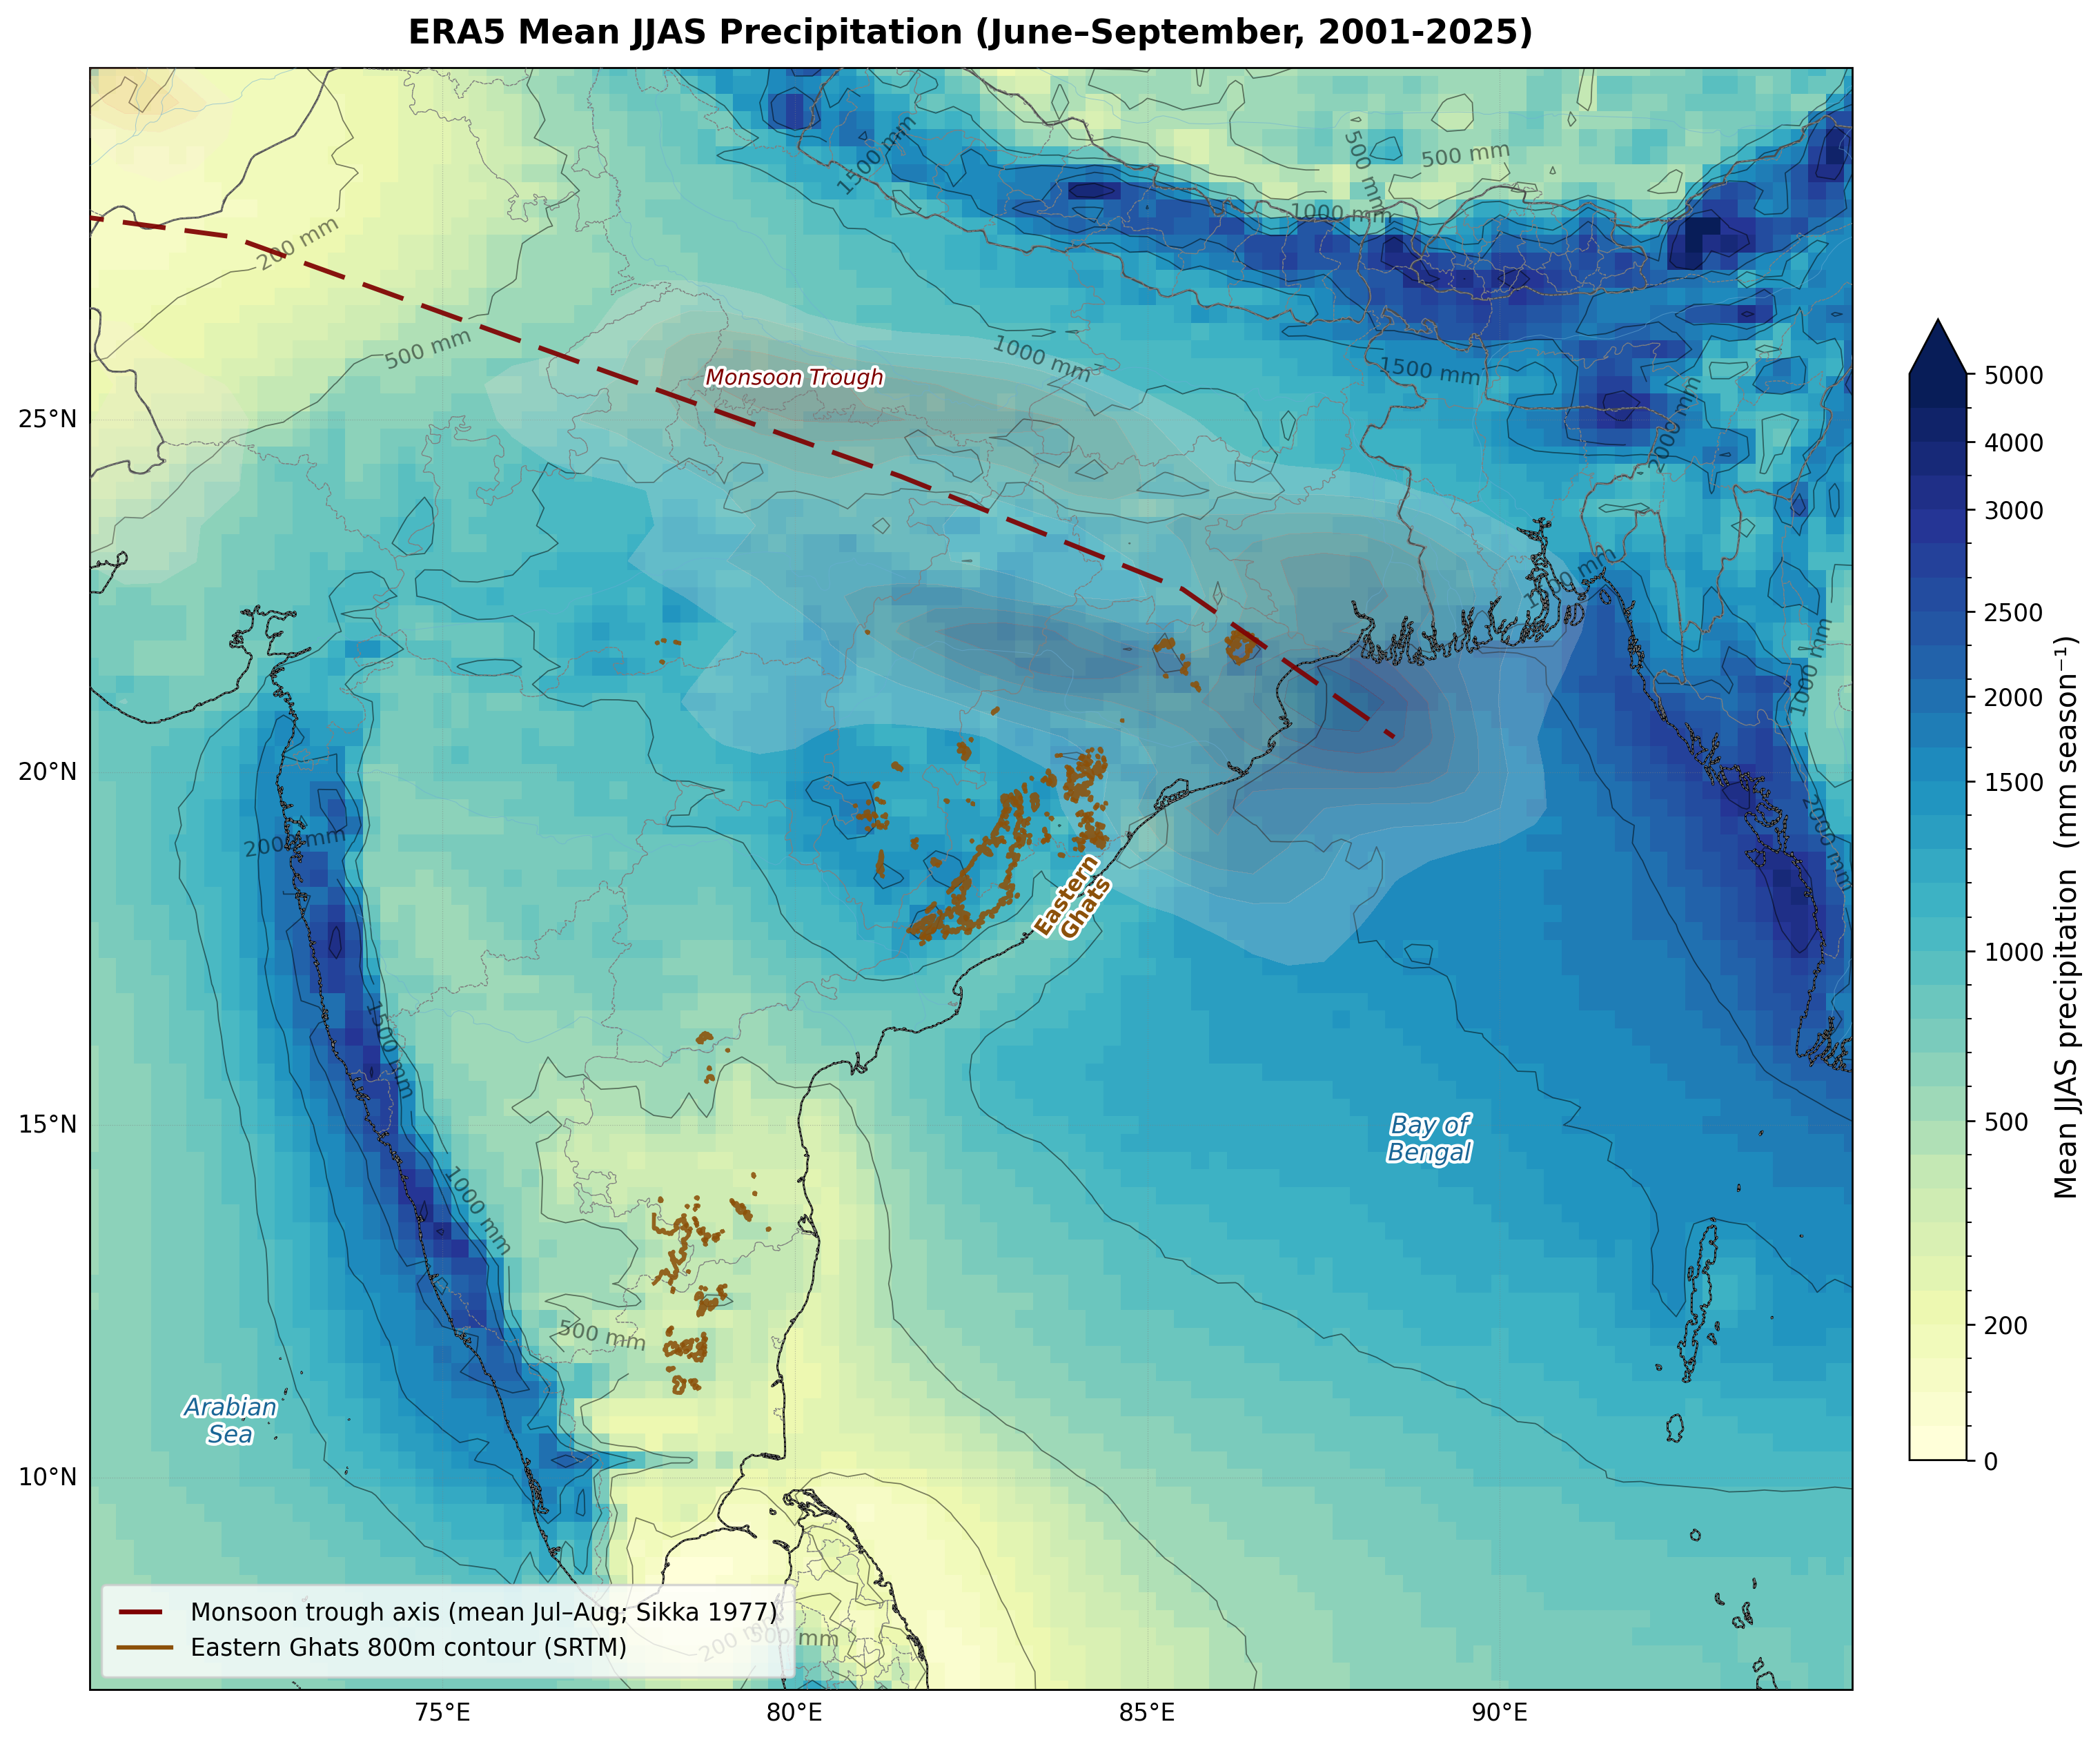
\includegraphics[width=0.9\textwidth]{india_jjas_climatology}
  \caption[JJAS seasonal rainfall climatology over India (2001-2025)]{Mean
  June-September precipitation (mm) over India from ERA5 (2001-2025).}
  \label{fig:india_rainfall_clim}
\end{figure}

% \section{Monsoon Depressions: Propagation, and the Post-Landfall Behavior}
\section{Monsoon Depressions \texorpdfstring{:}{} Propagation, and the Post-Landfall Behavior}
\label{sec:intro_md_problem}

Monsoon Depressions typically form over the Bay of Bengal (BoB)
during July and August, when warm sea-surface temperatures
(28-30$^\circ$C), deep atmospheric moisture, and strong low-level
cyclonic vorticity along the monsoon trough create favorable genesis
conditions. Historically, the BoB generates 5-6 MDs per year, with
substantial interannual variability tied to ENSO and Indian Ocean modes.

Before examining the post-landfall problem, it is useful to understand
two fundamental properties of these systems: why they rotate
anti-clockwise, and why they consistently track north-westward.

\subsection{Monsoon Depression Rotation}
\label{subsec:md_rotation}

All cyclonic weather systems in the Northern Hemisphere - including MDs -
rotate \emph{anti-clockwise} (cyclonically) as a direct consequence of the
\textbf{Coriolis force}. The Coriolis force is force arising from Earth's
rotation: in the Northern Hemisphere, any large-scale air parcel moving
toward a low-pressure center is deflected to its \emph{right}. This persistent
rightward deflection causes air flowing inward toward the low to curve
around it in a counter-clockwise sense, sustaining the cyclonic circulation
\autocite{holton2004introduction, sikka1977}. This is the same mechanism
responsible for the rotation of tropical cyclones, and even large eddies
in the ocean at sufficiently large scales.

In the case of an MD, the surface pressure minimum at the storm center
drives convergent inflow in the boundary layer. The Coriolis force
continuously deflects this inflow to the right, so that instead of
moving directly toward the center, air spirals cyclonically around it.
The Coriolis parameter $f = 2\Omega \sin\phi$ (where $\Omega$ is
Earth's angular velocity and $\phi$ is latitude) controls the strength
of this deflection: at the BoB and northern Indian latitudes
(10-25$^\circ$N), $f$ is large enough to enforce a well-organised
cyclonic vortex.

% Related images/webpages
% https://oceanservice.noaa.gov/education/tutorial_currents/04currents1.html
% https://www.weather.gov/source/zhu/ZHU_Training_Page/Miscellaneous/lowleveljet/lowleveljet.html
% Source for jet stream images:
% https://www.weather.gov/source/zhu/ZHU_Training_Page/Miscellaneous/lowleveljet/lowleveljet.html
\begin{figure}[H]
  \centering
  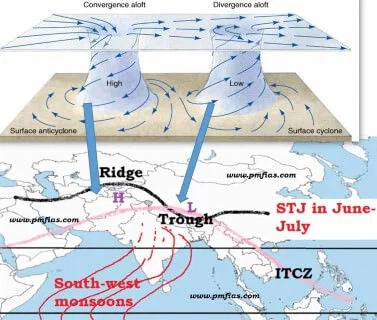
\includegraphics[width=0.75\textwidth]{Jet.png}
  \caption[Monsoon circulation]{The Sub-Tropical Westerly Jet (STJ)
    and its poleward retreat at monsoon onset, reducing vertical wind
    shear over the Bay of Bengal and
  permitting organised Monsoon Depression development.}
  \label{fig:Jet_stream_schematic_1}
\end{figure}

\subsection{Monsoon Depression North-Westward Propagation}
\label{subsec:md_propagation}

\begin{figure}[H]
  \centering
  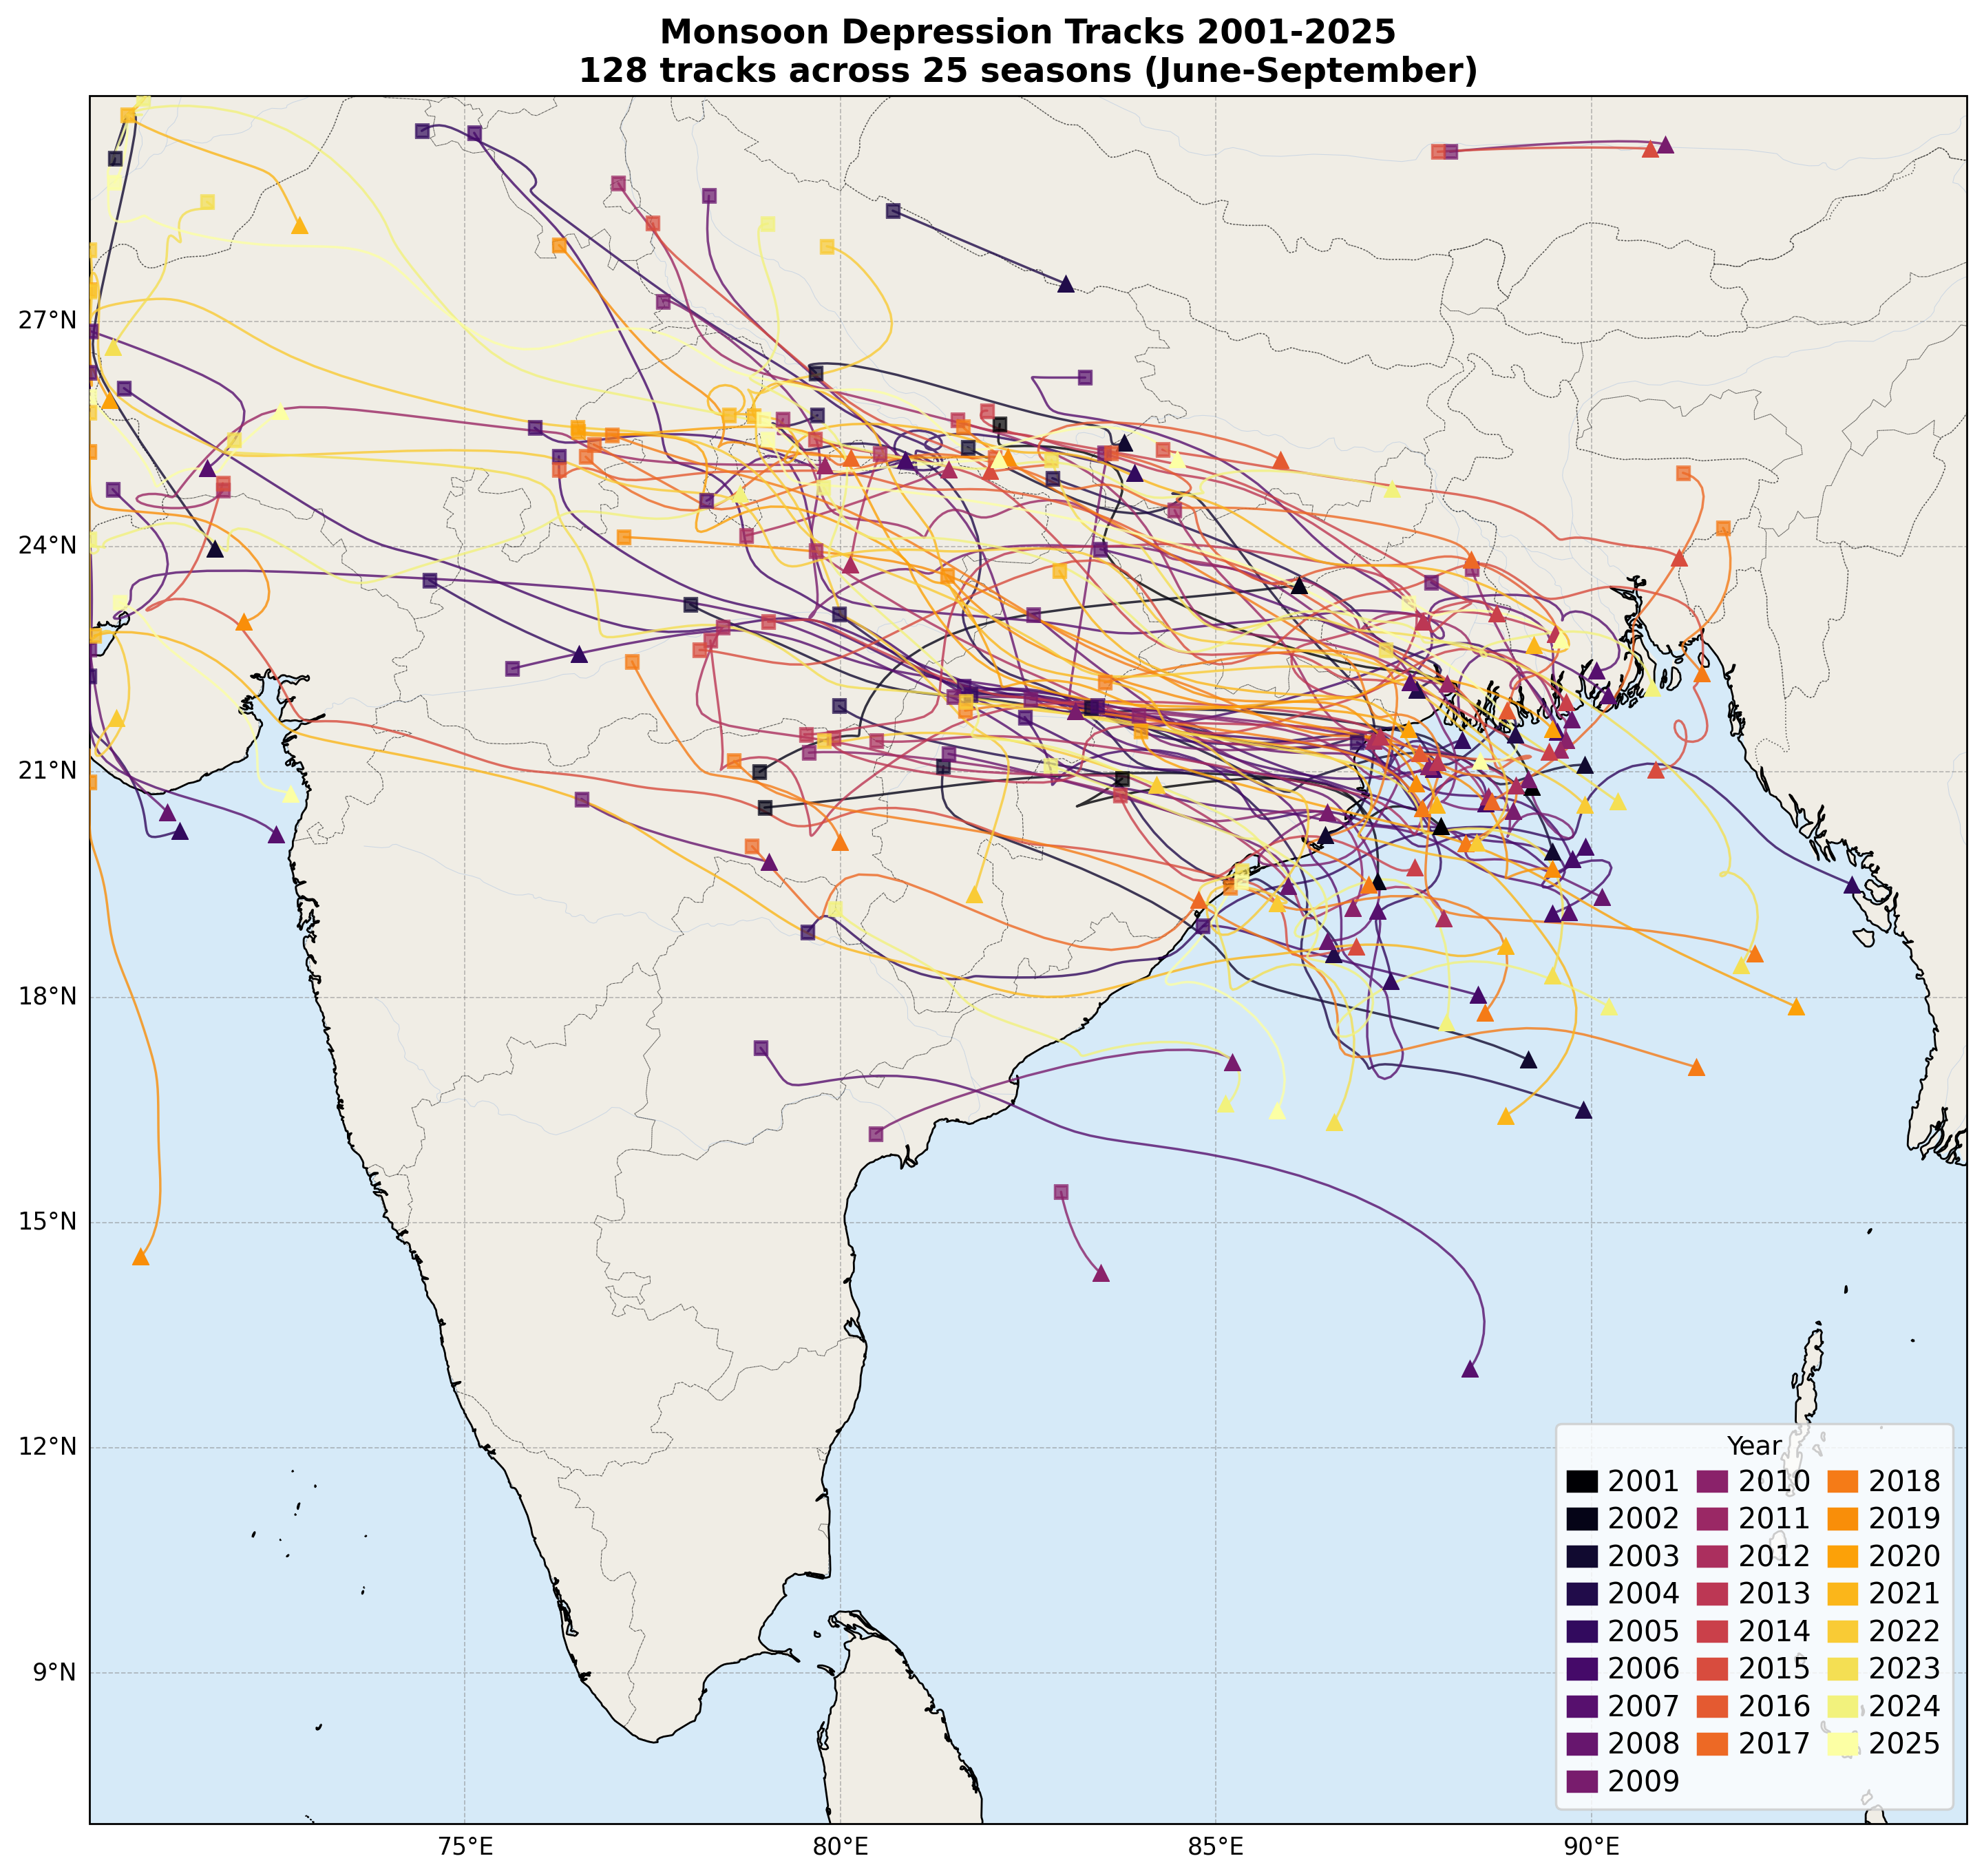
\includegraphics[width=0.9\textwidth]{all_years_tracks_map.png}
  \caption[Monsoon Propagation]{Monsoon depression detection from
  year 2001 to 2025}
  \label{fig:Monsoon_propagation}
\end{figure}

The characteristic north-westward translation of MDs results from the
following complementary mechanism operating on different scales

\begin{itemize}
  \item \textbf{Steering by the large-scale monsoon flow.} Once formed,
    an MD is steered predominantly by the mean environmental winds in
    the mid-troposphere (approximately the 500-700\,hPa layer). During
    the active ISM season, the large-scale monsoon circulation drives
    a mean westward and slightly northward flow across the BoB and
    northern India. The semi-permanent monsoon trough, extending from
    Pakistan across Rajasthan and central India to the BoB head,
    further guides the system along its north-westward axis
    \autocite{mishra2021monsoon, sikka1977}.
    % \item \textbf{The Somali Low-Level Jet and the Sub-Tropical Jet
    %   retreat.} The \textbf{Somali Low-Level Jet} (Findlater Jet), a
    %   powerful southwesterly stream at 850-925\,hPa
    %   \autocite{findlater1969}, intensifies during the active ISM and
    %   channels moisture from the Arabian Sea into the BoB. This jet
    %   also acts as a steering current, pushing disturbances
    %   north-westward into the Indian inland. At upper levels, the
    %   \textbf{Sub-Tropical Westerly Jet} retreats poleward of the
    %   Himalayas at monsoon onset \autocite{holton2004introduction},
    %   sharply reducing vertical wind shear over the BoB and permitting
    %   organised vortex development.
    % \item \textbf{Upper-level wind shear modulation.} At upper levels, the
    %   \textbf{Sub-Tropical Westerly Jet} (STJ) retreats poleward of the
    %   Himalayas at monsoon onset \autocite{holton2004introduction},
    %   sharply reducing vertical wind shear over the BoB and permitting
    %   organised vortex development.
\end{itemize}

The net effect of these steering mechanisms is a track directed
north-west (NW) or west-northwest (WNW) at translational speeds of
2-6\,m\,s$^{-1}$ (7-22\,km\,h$^{-1}$), making landfall preferentially
along the Odisha, West Bengal, and northern Andhra Pradesh coastlines.

Classical tropical meteorology theory predicts that a cyclonic system
should weaken rapidly upon crossing the coastline. Over the ocean,
the warm sea surface continuously restores latent and sensible heat
consumed by convection. As the system moves over land, this energy
source is removed. Surface friction simultaneously increases,
disrupting boundary-layer convergence and reducing the efficiency of
moisture transport into the inner core. Expected dissipation time is
24-48 hours after landfall - consistent with the decay observed in
most tropical cyclones.

In practice, a significant fraction of observed Indian MDs defies this
expectation. Cases in the 2001-2025 ERA5 detection record show systems
maintaining organised 850\,hPa vorticity and deep convection for 3-5
days and 800-1200\,km into the Indian inland. Understanding the physical
mechanisms enabling this persistence is a pressing operational
forecasting and climate impact problem.

% \section{The Brown Ocean Effect: Mechanism}
\section{The Brown Ocean Effect\texorpdfstring{:}{} Mechanism}
\label{sec:intro_boe}

\subsection{What is the Brown Ocean Effect?}
\label{subsec:boe_definition}

A compelling explanation for anomalous inland maintenance is the
\emph{Brown Ocean Effect} (BOE), first introduced and named by
\autocite{andersen2013}. The term ``Brown Ocean'' refers to the state
after a period of intense monsoon rainfall in which the saturated land
surface - visually brown and wet - mimics the energetic behaviour of a
warm tropical ocean. The BOE describes the process by which a
sufficiently wet land surface supplies \emph{latent heat flux} (LHF)
at rates comparable to a warm ocean, effectively replacing the oceanic
energy source after the MD makes landfall.

Over the ocean, sea-surface evaporation supplies latent heat to
sustain convection within the MD. When the storm crosses the coast,
it normally loses this energy supply. However, if the land surface
has been pre-moistened by antecedent monsoon rainfall to near field
capacity, the soil evaporates at the \emph{potential evaporation
rate} - the same rate as an ocean water surface - because water supply
is not limiting. The atmosphere above such a surface, the land
surface behaving thermodynamically like an ocean: high LHF, low Bowen
ratio (SHF/LHF), and a near-saturated boundary layer. This allows the MD's
convective organisation to persist for days after landfall.

\begin{figure}[H]
  \centering
  %% Right = ocean phase (evaporating blue ocean -> convection),
  %% Left = land phase (saturated brown soil -> comparable
  % evaporation -> convection),
  %% center = positive feedback loop arrow diagram)
  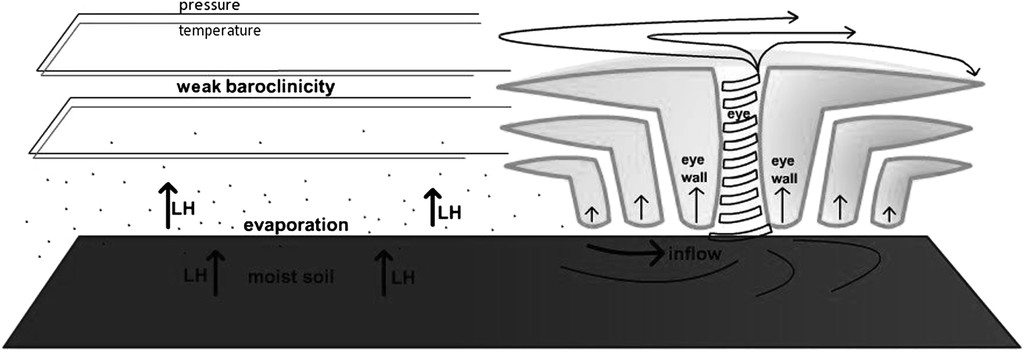
\includegraphics[width=0.8\textwidth]{BOE_schematic.jpg}
  \caption[Schematic of the Brown Ocean Effect mechanism]{The Brown
    Ocean Effect. Over pre-moistened land, saturated soil evaporates
    at the potential rate, sustaining LHF $\geq 70$\,W\,m$^{-2}$ and
  the precipitation-soil moisture feedback loop. Source: \autocite{andersen2013}.}
  \label{fig:boe_schematic}
\end{figure}

\subsection{The BOE Criterion}
\label{subsec:boe_criterion}

\cite{andersen2013} formalised the BOE with a measurable criterion:
\begin{equation}
  \text{LHF}_\text{inland} \geq 70\,\text{W\,m}^{-2}
  \quad \text{sustained for} \geq 18\,\text{consecutive hours after landfall.}
  \label{eq:boe_intro}
\end{equation}
This threshold of 70\,W\,m$^{-2}$ represents the minimum LHF that can
meaningfully sustain the moisture supply to deep convection within
the MD vortex. Systems meeting this criterion are termed \emph{BOE candidates}.

\subsection{Why the BOE Matters for Indian Monsoon Depressions}
\label{subsec:boe_significance}

The BOE is particularly significant in the Indian context for two reasons:
\begin{enumerate}
  \item \textbf{The BOE involves a self-reinforcing feedback loop.}
    The MD's own rainfall wets the soil beneath its track, which in
    turn sustains high LHF, which sustains subsequent convection and
    rainfall. This precipitation-soil moisture positive feedback
    (Figure~\ref{fig:boe_schematic}) means the BOE is not a passive
    response to antecedent conditions but an \emph{active} process
    that can maintain - and in some cases intensify - the surface
    energy supply during the land phase.
  \item \textbf{The land surface is pre-conditioned.} By July and
    August - peak MD months - the Gangetic plains and central India have
    received several weeks of monsoon rainfall, and near-surface soil
    moisture is frequently near field capacity. The land is ``charged''
    by antecedent rainfall before any MD arrives. This  \emph{antecedent
    soil moisture} effect - shown empirically by
    \autocite{kishtawal2013enhancement} to be predictor of inland penetration
    distance - is the critical enabling condition for the BOE over India.
\end{enumerate}

Without the BOE, post-landfall decay is controlled by surface
friction, reduced moisture flux, and the absence of oceanic thermal
forcing. With the BOE, the land surface functionally extends the
oceanic energy supply into the interior, explaining why certain MDs
persist for nearly a week and penetrate 1000-1200\,km inland.

The Eastern Ghats, however, introduce a complicating factor. This
discontinuous range of hills (600-1000\,m) along the eastern Deccan
margin intercepts the tracks of many landfalling MDs, slowing their
forward movement, enhancing windward precipitation, and potentially
disrupting the low-level moisture inflow that sustains inner-core
convection \autocite{houze1994}. Whether BOE-driven surface flux can
compensate for terrain-induced weakening and under what soil moisture
conditions is a key unresolved question motivating this thesis.

\section{Research Gap}
\label{sec:intro_gap}

Despite growing literature on the BOE in Atlantic and Gulf-coast
systems, and despite modelling and proxy evidence linking antecedent
soil moisture to Indian MD longevity \autocite{kishtawal2013enhancement,
osuri2020, hunt2017effect}, a systematic observational study of the
BOE in Indian MDs using storm-centerd diagnostics has not been
published. Previous Indian work relied on NWP experiments or
fixed-grid climatological correlations, without characterising the
azimuthal and radial evolution of LHF and soil moisture
\emph{relative to the moving storm center}. This storm-centerd
perspective is the primary methodological novelty of the present study.

\section{Research Objectives}
\label{sec:intro_objectives}

\begin{enumerate}
  \item Detect and characterise MD events from ERA5 over 2001-2025,
    validated against IMD reports, and classify them as short-lived
    ($<96$\,h) or long-lived ($\geq 96$\,h).
  \item Reconstruct the azimuthal and radial evolution of surface LHF,
    SHF, soil moisture (\texttt{SWVL1}), precipitation, and 2-m dew-point
    depression relative to the moving MD center via Azimuthal
    Hovm\"{o}ller analysis, comparing ocean and land phases.
    % \item Assess whether observed inland MDs satisfy the
    %   Andersen-Shepherd BOE criterion and document the landfall
    %   thermodynamic transitions distinguishing BOE candidates from
    %   conventionally decaying systems.
    % \item Quantify the role of antecedent soil moisture (exponentially
    %   weighted index over the future inland track corridor) in predicting
    %   inland penetration distance and post-landfall duration.
  \item Quantify the influence of antecedent soil moisture and
    terrain elevation. Characterise Eastern Ghats terrain influence
    on MD translational speed, precipitation asymmetry, and inland
    penetration using SRTM elevation data, and identify how this
    terrain interaction modulates the BOE.
\end{enumerate}

% \section{Thesis Organisation}
% \label{sec:intro_organisation}
%
% Chapter~\ref{ch:background} reviews tropical LPS energetics, MD
% structure and climatology, the BOE mechanism, land-atmosphere
% coupling, soil hydraulics, and Eastern Ghats orography.
% Chapter~\ref{ch:methodology} describes the ERA5 dataset, MD detection
% algorithm, Azimuthal Hovm\"{o}ller construction, time-series
% diagnostics, antecedent soil moisture index, heat flux analysis, and
% terrain characterisation.
% Chapter~\ref{ch:results} presents results in sequence: climatological
% overview $\rightarrow$ Hovm\"{o}ller diagnostics $\rightarrow$
% time-series thermodynamics $\rightarrow$ BOE classification
% $\rightarrow$ antecedent soil moisture $\rightarrow$ terrain interaction.
% Chapter~\ref{ch:discussion} synthesises these findings.
% Chapter~\ref{ch:conclusions} states the principal conclusions and
% future directions.
 %% Introduction
% Second Chapter: Background and Literature Review

\ifpdf
\graphicspath{{chapters/Figs/}{chapters/Figs/Raster/}{Figs/PDF/}{Figs/}}
\else
\graphicspath{{chapters/Figs/}{chapters/Figs/Vector/}{Figs/}}
\fi

\chapter{Scientific Background and Literature Review}
\label{ch:background}
\section{Tropical Low-Pressure Systems over the Bay of Bengal}
\label{sec:lps_overview}
\subsection{IMD Classification Hierarchy}
\label{subsec:imd_classification}

The India Meteorological Department classifies synoptic-scale
cyclonic systems over the north Indian Ocean in ascending order of
intensity based on maximum sustained surface wind speed: a \emph{Low}
(winds $<17$\,knots), \emph{Depression} (17-27\,knots), \emph{Deep
Depression} (28-33\,knots), \emph{Cyclonic Storm} (34-47\,knots), and
progressively stronger categories up to Super Cyclonic Storm ($>120$\,knots).

\emph{Monsoon Depressions} occupy the upper Depression category and
occasionally each Deep Depression intensity, but their dynamics and
thermodynamics are sufficiently distinct from tropical cyclones for
separate treatment.

The distinction is not merely one of intensity. MDs are embedded in,
and steered by, the large-scale monsoon circulation during the JJAS
season, whereas tropical cyclones typically develop in the relatively
quiescent pre-monsoon or post-monsoon environment when ambient
vertical wind shear is low.

MDs are characterised by a broader circulation, weaker tangential
winds, and a dual cold-core/warm-core thermal structure
\autocite{rashid2005track} that reflects their formation in a
moisture-laden, sheared monsoon environment.

\subsection{Energetics of Tropical Low-Pressure Systems}
\label{subsec:lps_energetics}

The energy source for all tropical LPS is latent heat released
through condensation in organised deep convection. Over the ocean,
the Warm Core Thermal Wind relationship maintains a pressure-gradient
force that drives surface boundary-layer convergence, which lifts
moisture-laden air into convective updrafts.
The surface enthalpy flux from the warm ocean-the sum of latent heat
flux (LHF) from evaporation and sensible heat flux (SHF) from
conduction-continuously replenishes this energy.

The \textbf{Bowen ratio ($\beta$)} quantifies the partitioning of
surface energy supply \autocite{trenberth2009earth}. Over the open ocean,
$\beta \approx 0.1$-$0.3$: the dominant energy transfer to the atmosphere
is latent heat. Over dry land, $\beta > 1$: sensible heating dominates.
Over saturated land (near-field-capacity soil), $\beta$ can approach
oceanic values.
\begin{equation}
  \beta = Q_H / Q_E
\end{equation}
where $Q_H$ is SHF and $Q_E$ is LHF.

This is the thermodynamic core of the Brown Ocean Effect, a sufficiently
wet land surface has a Bowen ratio indistinguishable from an ocean.

\section{Dynamics of Monsoon Depression Motion}
\label{sec:md_dynamics}

\subsection{Why Monsoon Depressions Rotate Anti-Clockwise}
\label{subsec:md_anticlockwise}

All synoptic-scale cyclonic systems in the Northern Hemisphere rotate
anti-clockwise as a direct consequence of the \textbf{Coriolis force},
an apparent deflection arising from Earth's rotation that acts perpendicular
to and to the \emph{right} of any moving air parcel in the Northern Hemisphere.
The Coriolis parameter at latitude $\phi$ is:
\begin{equation}
  f = 2\Omega\sin\phi,
  \label{eq:coriolis_bg}
\end{equation}
where $\Omega = 7.292 \times 10^{-5}$\,rad\,s$^{-1}$. At the typical genesis
latitudes of BoB MDs (10-20$^\circ$N), $f \approx 2.5$-$5.0 \times
10^{-5}$\,s$^{-1}$.

\begin{figure}[H]
  \centering
  %% DRAW THIS FIGURE - Coriolis deflection schematic
  %% Show: circular low-pressure center, 4 straight inward arrows (N/S/E/W),
  %% each curving rightward to produce CCW rotation. Label f = 2Ω sinφ.
  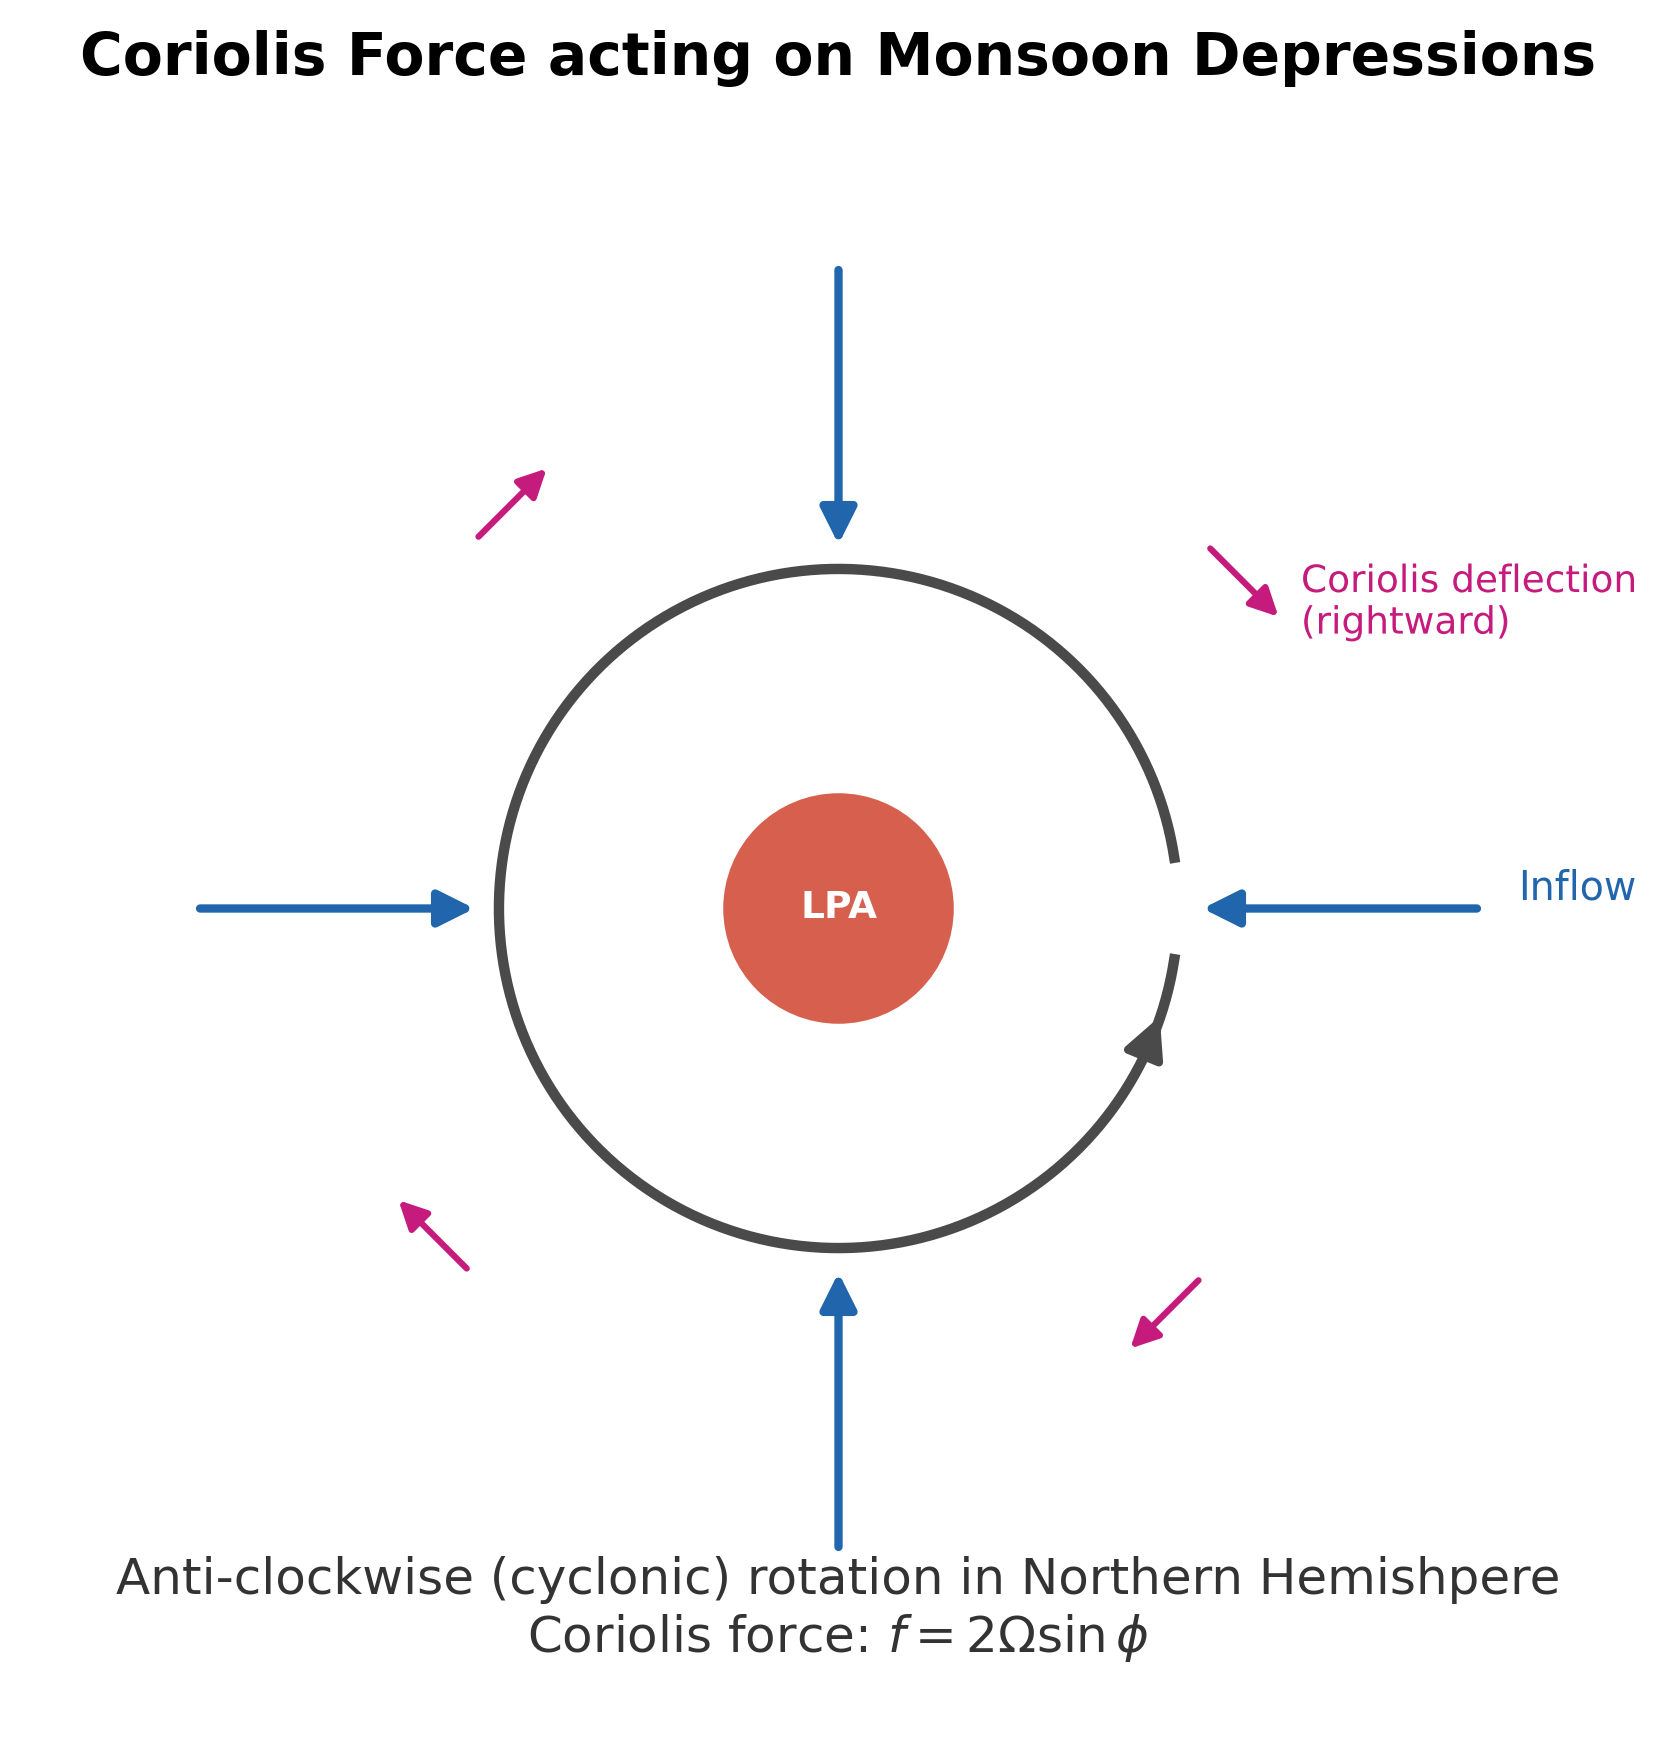
\includegraphics[width=0.7\textwidth]{coriolis_md_rotation.png}
  % \caption[Coriolis force and cyclonic rotation in the Northern
  % Hemisphere]{The Coriolis force deflects air parcels to the right in the
  % Northern Hemisphere. Air drawn toward a surface low (white arrows) is
  % continuously deflected, producing anti-clockwise cyclonic rotation (curved arrows).}
  \caption[Coriolis force producing anti-clockwise MD
  rotation]{Boundary-layer air converging toward the MD center is
    deflected rightward by the Coriolis force, producing an
    anti-clockwise (cyclonic) circulation. The Coriolis parameter ($f =
  2\Omega\sin\phi$) increases with latitude.}%, setting the minimum
  % latitude ($\sim 5^\circ$N) for organised vortex development.}
  \label{fig:coriolis_bg}
\end{figure}

When a surface pressure minimum forms over the BoB, typically through
barotropic instability along the monsoon trough \autocite{mishra2021monsoon},
the surrounding air converges toward the center. As each
inward-flowing air parcel is continuously deflected to the right by
the Coriolis force, the resulting organised inflow spirals
anti-clockwise around the low. This anti-clockwise circulation is
maintained in gradient balance: the inward pressure-gradient
force directed toward the low is balanced at each level by the
Coriolis force and centrifugal acceleration acting outward. The
result is a self-sustaining cyclonic vortex whose circulation is
energetically driven by surface energy fluxes from below and latent
heating from deep convection above \autocite{holton2004introduction}.

% \subsection{Why Monsoon Depressions Track North-Westward: The Role of
% Jet Streams}
% \label{subsec:md_nw_track}
%
% The characteristic north-westward translation of Indian MDs at
% 2-6\,m\,s$^{-1}$ results from two overlapping large-scale
% atmospheric controls, both of which are unique to the active Indian
% summer monsoon period.

\subsubsection{The Monsoon Mean Flow and Trough Steering}

An MD embedded in the lower troposphere is advected by the
depth-averaged environmental wind in the 500-700\,hPa steering layer.
During June-September, the large-scale monsoon circulation drives
this steering flow broadly westward  and slightly poleward across the
BoB and northern India. The \textbf{monsoon trough}, a semi-permanent
axis of low pressure and enhanced cyclonic vorticity extending from
the Pakistan-Rajasthan border, across Uttar Pradesh and Madhya
Pradesh, to the BoB head-acts as the preferred corridor for LPS
propagation, guiding systems north-westward along its axis
\autocite{sikka1977, mishra2021monsoon}. Systems forming at the BoB head
are steered directly along this trough axis toward the
Odisha-Gangetic plain coast.
%
% \subsubsection{The Somali Low-Level Jet and Sub-Tropical Westerly Jet}
% \label{subsubsec:jet_streams}
%
% Two jet systems exert decisive control on MD development and motion
% (Figure~\ref{fig:jet_streams_schematic}):
%
% \textbf{(1) The Somali Low-Level Jet (Findlater Jet):} This
% powerful south-westerly jet at 850-925\,hPa, first documented by
% \autocite{findlater1969}, intensifies dramatically during the active
% ISM as the inter-hemispheric pressure gradient between the southern
% Indian Ocean and the heating Asian landmass maximises.
%
% The Findlater Jet channels large quantities of moisture-laden air
% from the Arabian Sea across the Indian peninsula into the BoB. In
% addition to its moisture supply role, the jet provides a powerful
% low-level steering current directed north-westward, which directly
% advects developing disturbances from the BoB head into the Indian
% interior. The jet core at 850\,hPa attains wind speeds of
% 20-30\,m\,s$^{-1}$ during active ISM spells and is the primary
% reason that MD tracks are so consistently directed toward Odisha,
% West Bengal, and Bihar rather than making arbitrary landfall along
% other coast segments.
%
% \textbf{(2) The Sub-Tropical Westerly Jet (STJ) and its poleward
% retreat:} During the pre-monsoon period (April-May), the STJ is
% positioned over northern India at approximately 200\,hPa, producing
% strong westerly vertical wind shear throughout the troposphere.
% This shear suppresses deep convective organisation and precludes MD
% development. As the monsoon onset occurs in June, the STJ abruptly
% jumps northward to a position at approximately 35-45$^\circ$N,
% entirely north of the Himalayas. With the STJ poleward of the
% Himalayan barrier, the upper-troposphere over the BoB and northern
% India becomes effectively \emph{decoupled} from the strong westerly
% shear. The resulting low-shear environment ($<10$\,m\,s$^{-1}$ over
% the BoB) is a necessary condition for MD deepening: a developing
% vortex is not ``sheared apart'' before it can organise
% \autocite{holton2004introduction}. The monsoon onset therefore acts as
% a switch that simultaneously provides moisture (via the LLJ),
% reduces shear (via the STJ retreat), and establishes the monsoon
% trough axis along which MDs will propagate.
%
% % FIX: include better image
% \begin{figure}[H]
%   \centering
%   %% Note: DRAW THIS FIGURE - jet stream schematic
%   %% Elements to include:
%   %%   Thick blue arrow: Somali/Findlater Jet at 850 hPa (SW to NE
%   % across Indian Ocean + India)
%   %%   Thin red arrow: STJ poleward of Himalayan barrier at 200 hPa
%   %%   Cyclone symbol: over Bay of Bengal
%   %%   NW arrow: MD track direction
%   %%   Dashed line: monsoon trough axis across northern India
%   %%   Grey arc: Himalayan range
%   % \fbox{\rule{0pt}{5.5cm}\rule{0.75\textwidth}{0pt}}
%   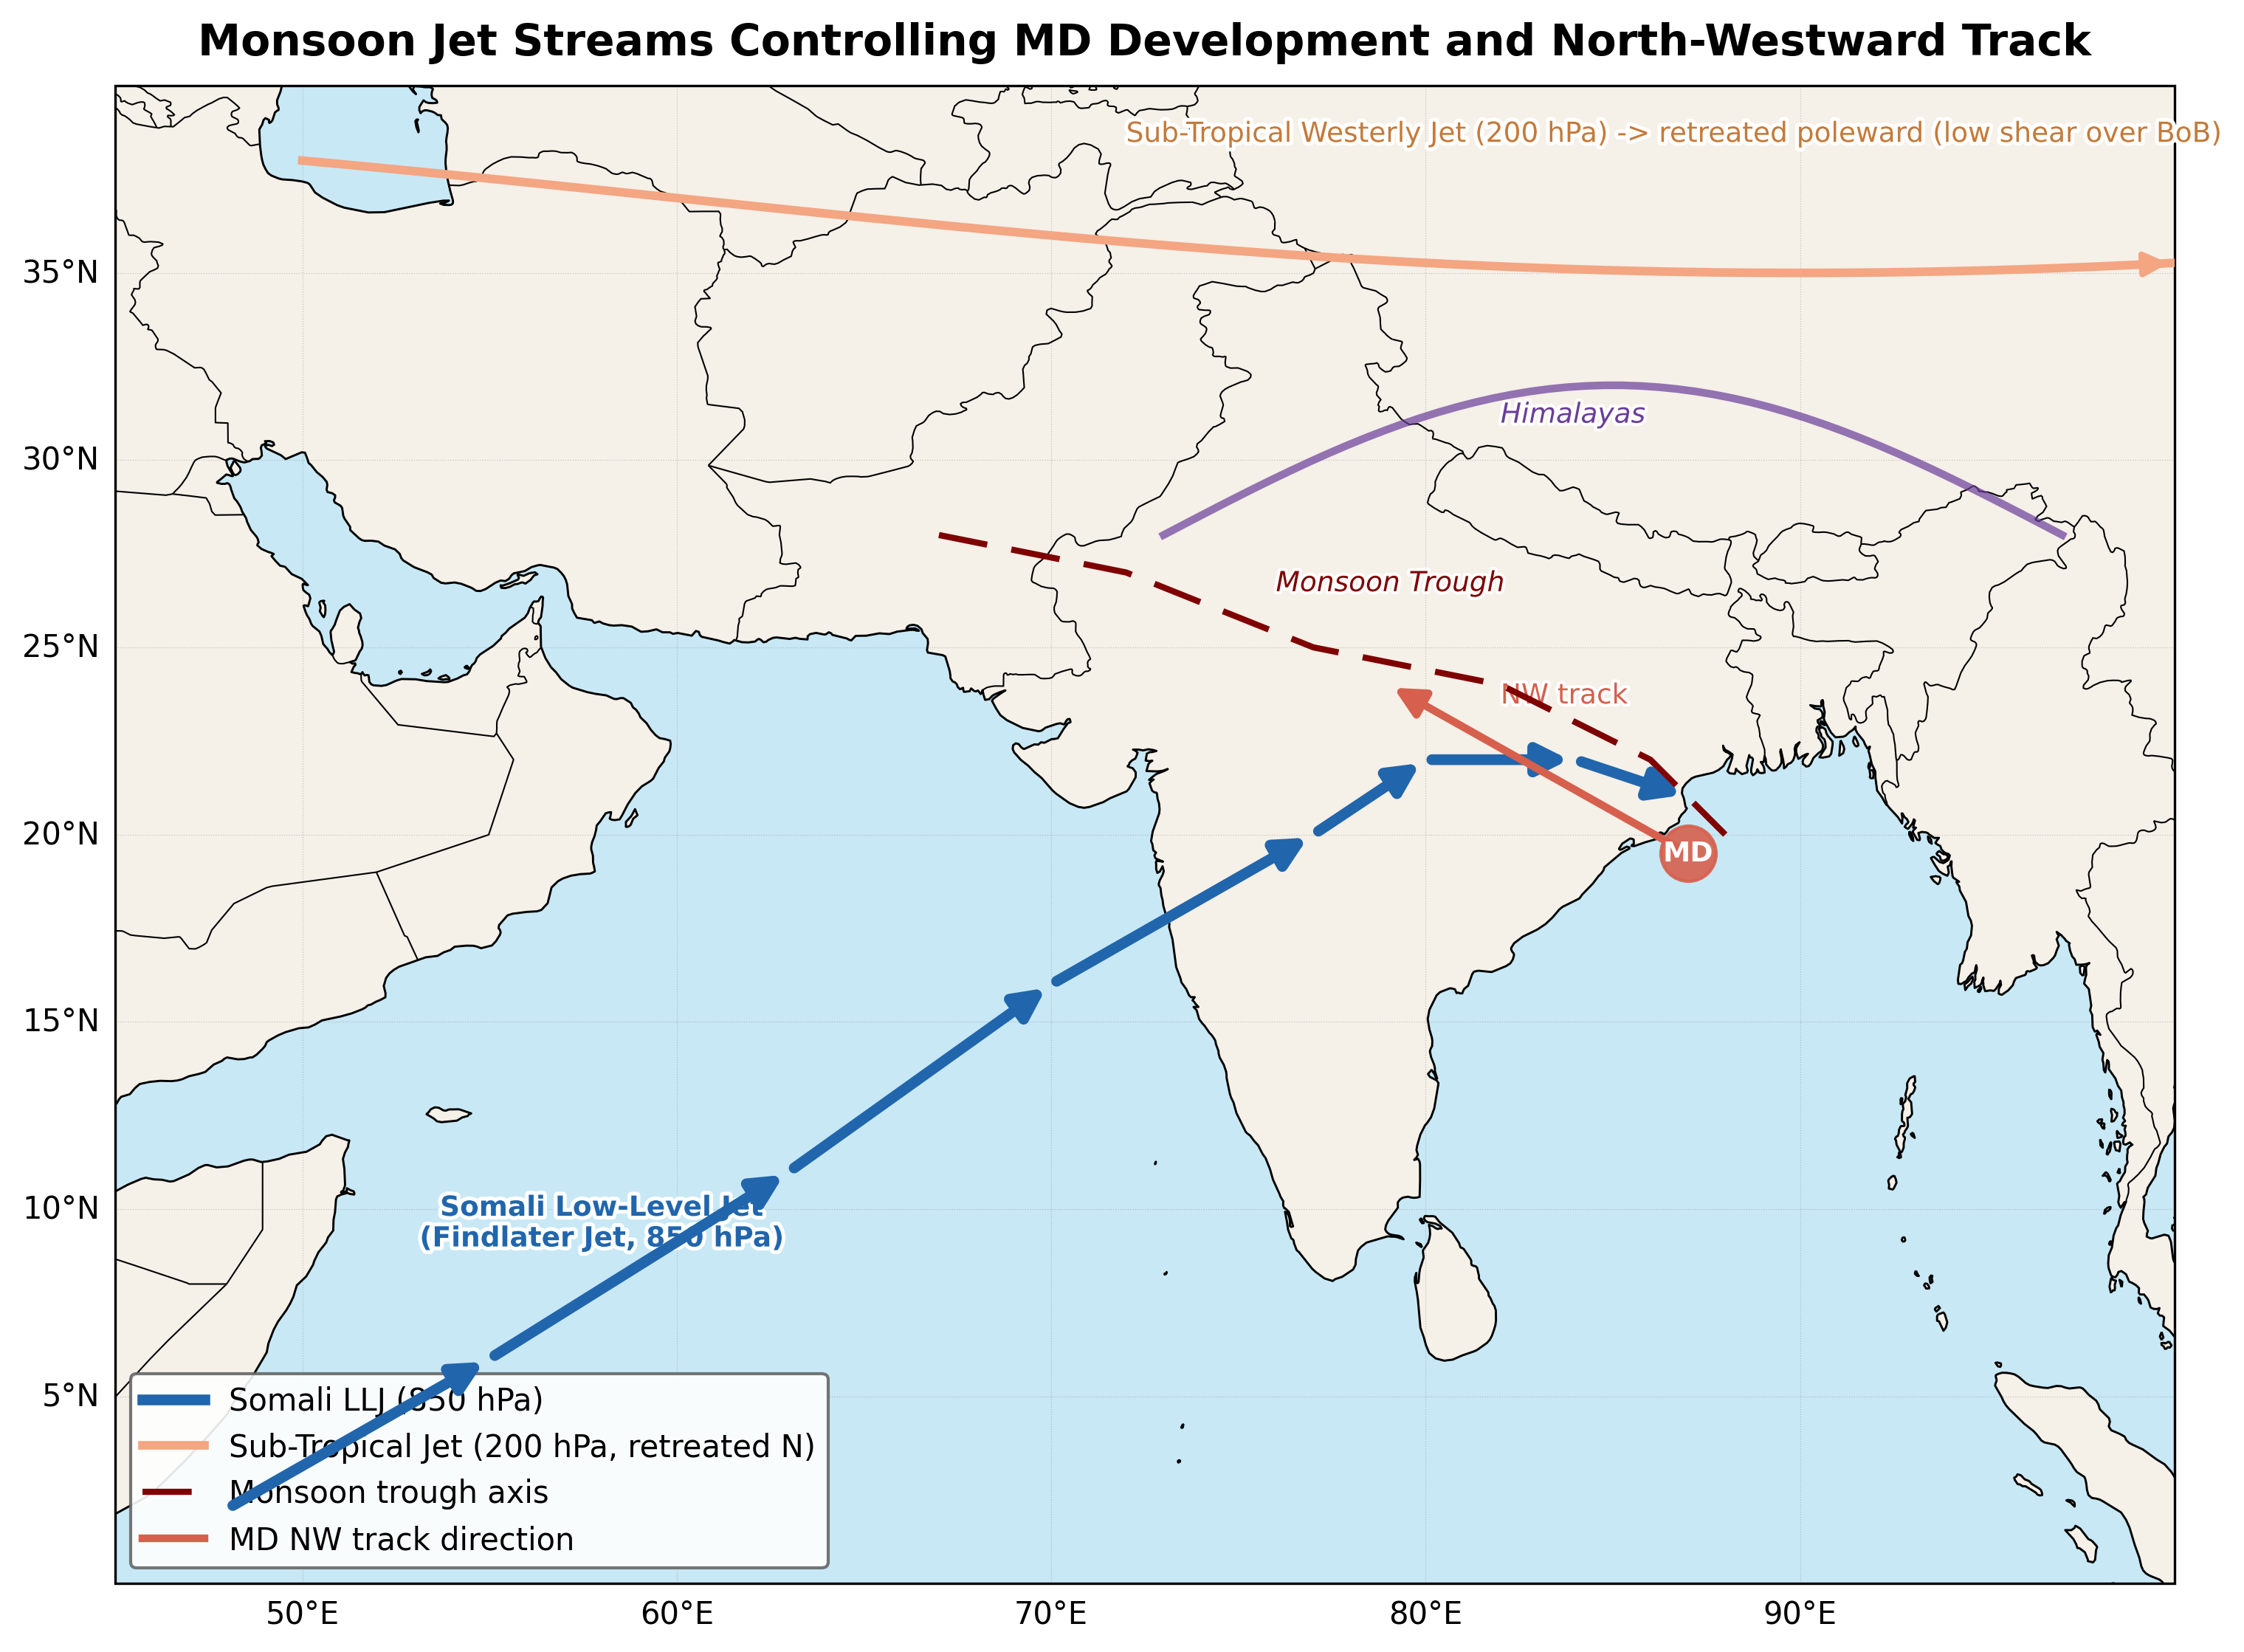
\includegraphics[width=0.75\textwidth]{jet_streams_schematic.png}
%   \caption[Monsoon jet streams controlling MD development and
%   north-westward motion]{Schematic showing the two jet systems
%     governing MD motion. The Somali Low-Level Jet (LLJ, thick arrow,
%     850\,hPa) supplies moisture and steers disturbances north-westward.
%     The Sub-Tropical Westerly Jet (STJ, thin arrow, 200\,hPa) has
%     retreated poleward of the Himalayas, eliminating destructive
%     upper-level wind shear over the BoB. The monsoon trough axis
%     (dashed) provides the preferred propagation corridor. After
%   \autocite{findlater1969} and \autocite{mishra2021monsoon}.}
%   \label{fig:jet_streams_schematic}
% \end{figure}

% \subsection{Vortex Tilt: The Structural Integrity Diagnostic}
\subsection{Vortex Tilt\texorpdfstring{:}{} The Structural Integrity Diagnostic}
\label{subsec:vortex_tilt_background}

As an MD translates inland, the environmental vertical wind shear and
terrain-induced boundary-layer friction can cause the vortex to tilt:
the low-level (850\,hPa) center displaces relative to the upper-level
(200-300\,hPa) warm core.

\autocite{rashid2005track} showed that a mature MD in the BoB typically
exhibits a small westward-northwestward tilt of 50-200\,km, the
direction dictated by the mean shear vector. This tilt is sustainable
so long as organised convection couples the upper and lower parts of
the vortex column through latent heat release.

After landfall, increased surface roughness decelerates the low-level
center faster than the upper-level flow, forcing the tilt to
increase. Once tilt exceeds a critical threshold, the
latent-heat-driven warm core decouples from the surface convergence
zone, convection weakens, and the vortex column rapidly loses
coherence-a structural precursor to terminal decay. The Brown Ocean
Effect counteracts this by sustaining boundary-layer convergence
(through continuous LHF) at the low-level center, keeping the
coupling alive even when the upper-level flow has advected the upper
warm core forward.

\section{The Brown Ocean Effect (BOE)\texorpdfstring{:}{} Mechanism and Prior Literature}
\label{sec:boe_literature}

\subsection{Definition and Evidence}
\label{subsec:boe_original}

The BOE was formally introduced and named by \autocite{andersen2013} in a global
climatological analysis of inland tropical cyclone maintenance events. They
identified numerous cases in which tropical systems over the continental United
States maintained or intensified over land and showed that these were associated
with sustained inland LHF meeting the criterion:
\begin{equation}
  \text{LHF}_{\text{inland}} \geq 70\;\text{W\,m}^{-2}
  \quad\text{for}\;\geq 18\;\text{consecutive hours post-landfall.}
  \label{eq:boe_def}
\end{equation}

% \yellownote{Add Tropical Storm Erin (2007) in reference and fix cite}
The canonical case study is Tropical Storm Erin (2007), which
unexpectedly re-intensified over Oklahoma to near-tropical-storm
intensity \autocite{andersen2014insights}. Post-analysis revealed that
the Southern Great Plains had been saturated by heavy antecedent
rainfall, providing LHF at rates comparable to the Gulf of Mexico.

% \yellownote{Add Tropical Storm Bill (2015) in reference and fix cite}
\autocite{wakefield2021} examined Tropical Storm Bill (2015) in detail
and provided the most complete documented case of the BOE feedback
loop, soil moisture near saturation at landfall maintained LHF
$>100$\,W\,m$^{-2}$, % which maintained CAPE,
which maintained organised precipitation that further wetted the
soil. The self-reinforcing character of this loop was identified as
the key mechanism enabling multi-day inland persistence.

\autocite{nair2019influence} demonstrated the sensitivity of BOE
intensity to land cover type, urbanised and irrigated agricultural
surfaces enhanced the BOE signal relative to natural vegetation, a
finding relevant to the heavily irrigated Indo-Gangetic plains (IGP).

\subsection{BOE Evidence in the Indian Context}
\label{subsec:boe_india}

The translation of the BOE concept to Indian Monsoon Depressions is
recent and mostly model-based. \autocite{kishtawal2013enhancement}
provided the first indirect observational evidence, using pre-storm
rainfall as a proxy for antecedent soil moisture, they demonstrated a
statistically significant positive relationship between the 15-day
pre-landfall cumulative rainfall along the future MD track corridor
and the subsequent inland penetration distance for 12 BoB depression
events. Their key finding were, heavier pre-storm rainfall (wetter
antecedent soil) produced longer inland persistence, is exactly what
the BOE predicts, but the mechanism (the LHF signal) was not directly
measurable from their proxy.

\autocite{hunt2017effect} used a numerical weather prediction model to
systematically perturb the soil moisture initialisation for simulated
MDs. They found that higher soil moisture led to a warmer
mid-tropospheric core, enhanced precipitation, and longer inland life
cycles, confirming the mechanistic link between surface state and MD
post-landfall dynamics in a model framework.

\autocite{osuri2020} demonstrated that assimilating satellite-derived
soil moisture (ASCAT) into the NWP initialisation significantly
improved simulated MD track and intensity, confirming the operational
relevance of the surface moisture state.

\autocite{vijay2024boe} applied the BOE framework to the catastrophic
1999 Odisha Supercyclone, showing that antecedent soil moisture
pre-conditioned by a previous tropical system played a role in the
rapid intensification near and after landfall.

This study closes the gap between these proxy-based and modelling
approaches by directly measuring the LHF signal in ERA5 reanalysis
through the storm-centered Azimuthal Hovm\"{o}ller diagnostic.

%% \section{Antecedent Soil Moisture: Pre-Conditioning and Soil Moisture Memory}
% \section{Antecedent Soil Moisture\texorpdfstring{:}{} Pre-Conditioning and Soil Moisture Memory}
% \label{sec:soil_moisture_bg}
%
% \subsection{The Soil Moisture Evaporation Regime Transition}
% \label{subsec:sm_regime}
%
% The relationship between soil moisture and surface evaporation rate
% is non-linear and threshold-controlled
% \autocite{seneviratne2010investigating}. Two regimes operate:
%
% \begin{enumerate}
%   \item \textbf{Water-limited regime} (dry soil, $\theta <
% \theta_\text{crit}$):
%     Evaporation is limited by the availability of soil water, not by
%     the available solar energy. LHF is proportional to $\theta /
%     \theta_\text{crit}$. In this regime, rainfall primarily
%     infiltrates into the soil (replenishing the deficit) rather than
%     evaporating immediately. Consequently, even heavy MD
%     precipitation may not raise LHF to BOE-sustaining levels if the
%     antecedent soil is very dry.
%   \item \textbf{Energy-limited regime} (wet soil, $\theta \geq
%     \theta_\text{crit}$): Soil is evaporating at its potential rate,
%     constrained only by the available net radiation, not by soil
%     water supply. LHF is at its maximum possible value for a given atmospheric
%     state, comparable to evaporation from an open water surface. This
%     is the regime in which the BOE operates. The critical threshold
%     $\theta_\text{crit}$ is approximately 65-75\,\% of the
%     soil's water holding capacity, corresponding to the matric
%     suction level at which hydraulic conductivity
%     begins to fall steeply \autocite{clapp1978empirical}.
% \end{enumerate}
%
% For Gangetic clay loam-the dominant soil texture along the preferred
% MD track corridor over northern India-the Clapp-Hornberger exponent
% $\beta \approx 7.12$ \autocite{clapp1978empirical}, implying that
% drainage slows dramatically as the soil approaches saturation and
% that near-saturated conditions ($\theta \geq \theta_\text{crit}$) are
% maintained for many days after heavy rainfall. This high soil
% moisture memory is precisely what enables multi-day BOE episodes:
% unlike sandy soils that drain and dry within hours, Gangetic clay
% loam retains near-capacity moisture for 3-7 days
% \autocite{seneviratne2010investigating}.

\subsection{The Precipitation-Soil Moisture Positive Feedback}
\label{subsec:precip_sm_feedback}

The soil moisture feedback to precipitation-whereby wet soil produces
enhanced surface evaporation, which moistens and destabilises the
boundary layer, which intensifies convection and precipitation-is
observationally established over India at synoptic and intra-seasonal
timescales \autocite{longterm2025, wei2016impact}.
The mechanism proceeds through two pathways:

\begin{enumerate}
  \item \textbf{Thermodynamic pathway:} Moist soil suppresses daytime
    sensible heating (lowering Bowen ratio$\beta$), reducing the height of the
    convective boundary layer and increasing near-surface specific humidity $q$.
    This raises the equivalent potential temperature ($\theta_e$)
    \autocite{bolton1980computation} at the surface, increasing CAPE and
    convective triggering probability.
    \begin{equation}
      \theta_e = T_K(P_0/P)^{R_d/c_p}\exp(L_v q / c_p T_L)
    \end{equation}
    where:\\
    $T_K$ is the absolute temperature at pressure $P$, \\
    $P_0$ is the reference pressure (usually 1000 hPa), \\
    $R_d$ is the gas constant for dry air, \\
    $c_p$ is the specific heat of dry air at constant pressure, \\
    $L_v$ is the latent heat of vaporization, \\
    $q$ is the specific humidity, \\
    $T_L$ is the temperature at the lifting condensation level.
  \item \textbf{Dynamic pathway:} Enhanced LHF at the land surface
    increases the low-level moisture flux convergence into the MD
    vortex-a process directly analogous to the oceanic surface flux
    maintaining the vortex over the BoB.
    % The key observational test implemented in this study, is the
    % Granger causality of total precipitation on subsequent SWVL1: if
    % precipitation significantly Granger-causes soil moisture (with
    % the expected positive sign), the active self-wetting component of
    % the BOE is confirmed in the ERA5 record.
    % \yellownote{TODO: Granger tests}
\end{enumerate}

% \subsection{The ASMI as a Pre-Landfall Predictor}
% \label{subsec:asmi_background}
%
% Building on \autocite{kishtawal2013enhancement}, this study employs an
% \emph{exponentially weighted} Antecedent Soil Moisture Index (ASMI)
% that (i) uses direct ERA5 \texttt{SWVL1} measurements rather than
% precipitation proxies, (ii) weights recent soil moisture more heavily
% than older conditions ($\kappa^d$, $\kappa = 0.85$), and (iii)
% computes the index specifically over the \emph{future inland track
% corridor} rather than the current position.
%
% The 7-day lag is theoretically motivated: it corresponds to the
% dominant soil moisture memory timescale of Gangetic clay loam (3-7
% days), meaning that the soil moisture 7 days before landfall best
% represents the background wetness state rather than being
% contaminated by either the MD's own recent rainfall or ephemeral dry spells.

\section{The Eastern Ghats: Orographic Barrier and Research Finding}
\label{sec:eastern_ghats_bg}

\subsection{Physical Geography and Structure}
\label{subsec:ghats_geography}

The Eastern Ghats are a discontinuous range of hills running
approximately north-northeast to south-southwest along the eastern
margin of the Deccan Plateau, at a general inland distance of
100-300\,km from the Bay of Bengal coast (Figure~\ref{fig:eastern_ghats_map}).

Unlike the continuous, high-elevation Western Ghats (2000-2500\,m),
the Eastern Ghats are fragmented by major river systems-the Mahanadi,
Godavari, and Brahmani rivers cross the range through wide
river-valley gaps-with typical average elevations of 600-1000\,m
(with highest peaks reaches around 1600\,m). The overall range width
is approximately 80-200\,km, and the mean slope angle of the windward
(eastern) face is shallow (1-3$^\circ$), making the Ghats moderate
rather than catastrophic orographic barrier. This geographic
structure has a critical implication for MD dynamics: the Ghats are
wide enough and high enough to impose significant orographic forcing,
yet gaps are wide enough to sometimes allow MD's low-level
circulation to partially pass through without the full brunt of
barrier blocking-making the \emph{landfall longitude} relative to gap
positions a potentially important predictor of inland penetration.

\begin{figure}[H]
  \centering
  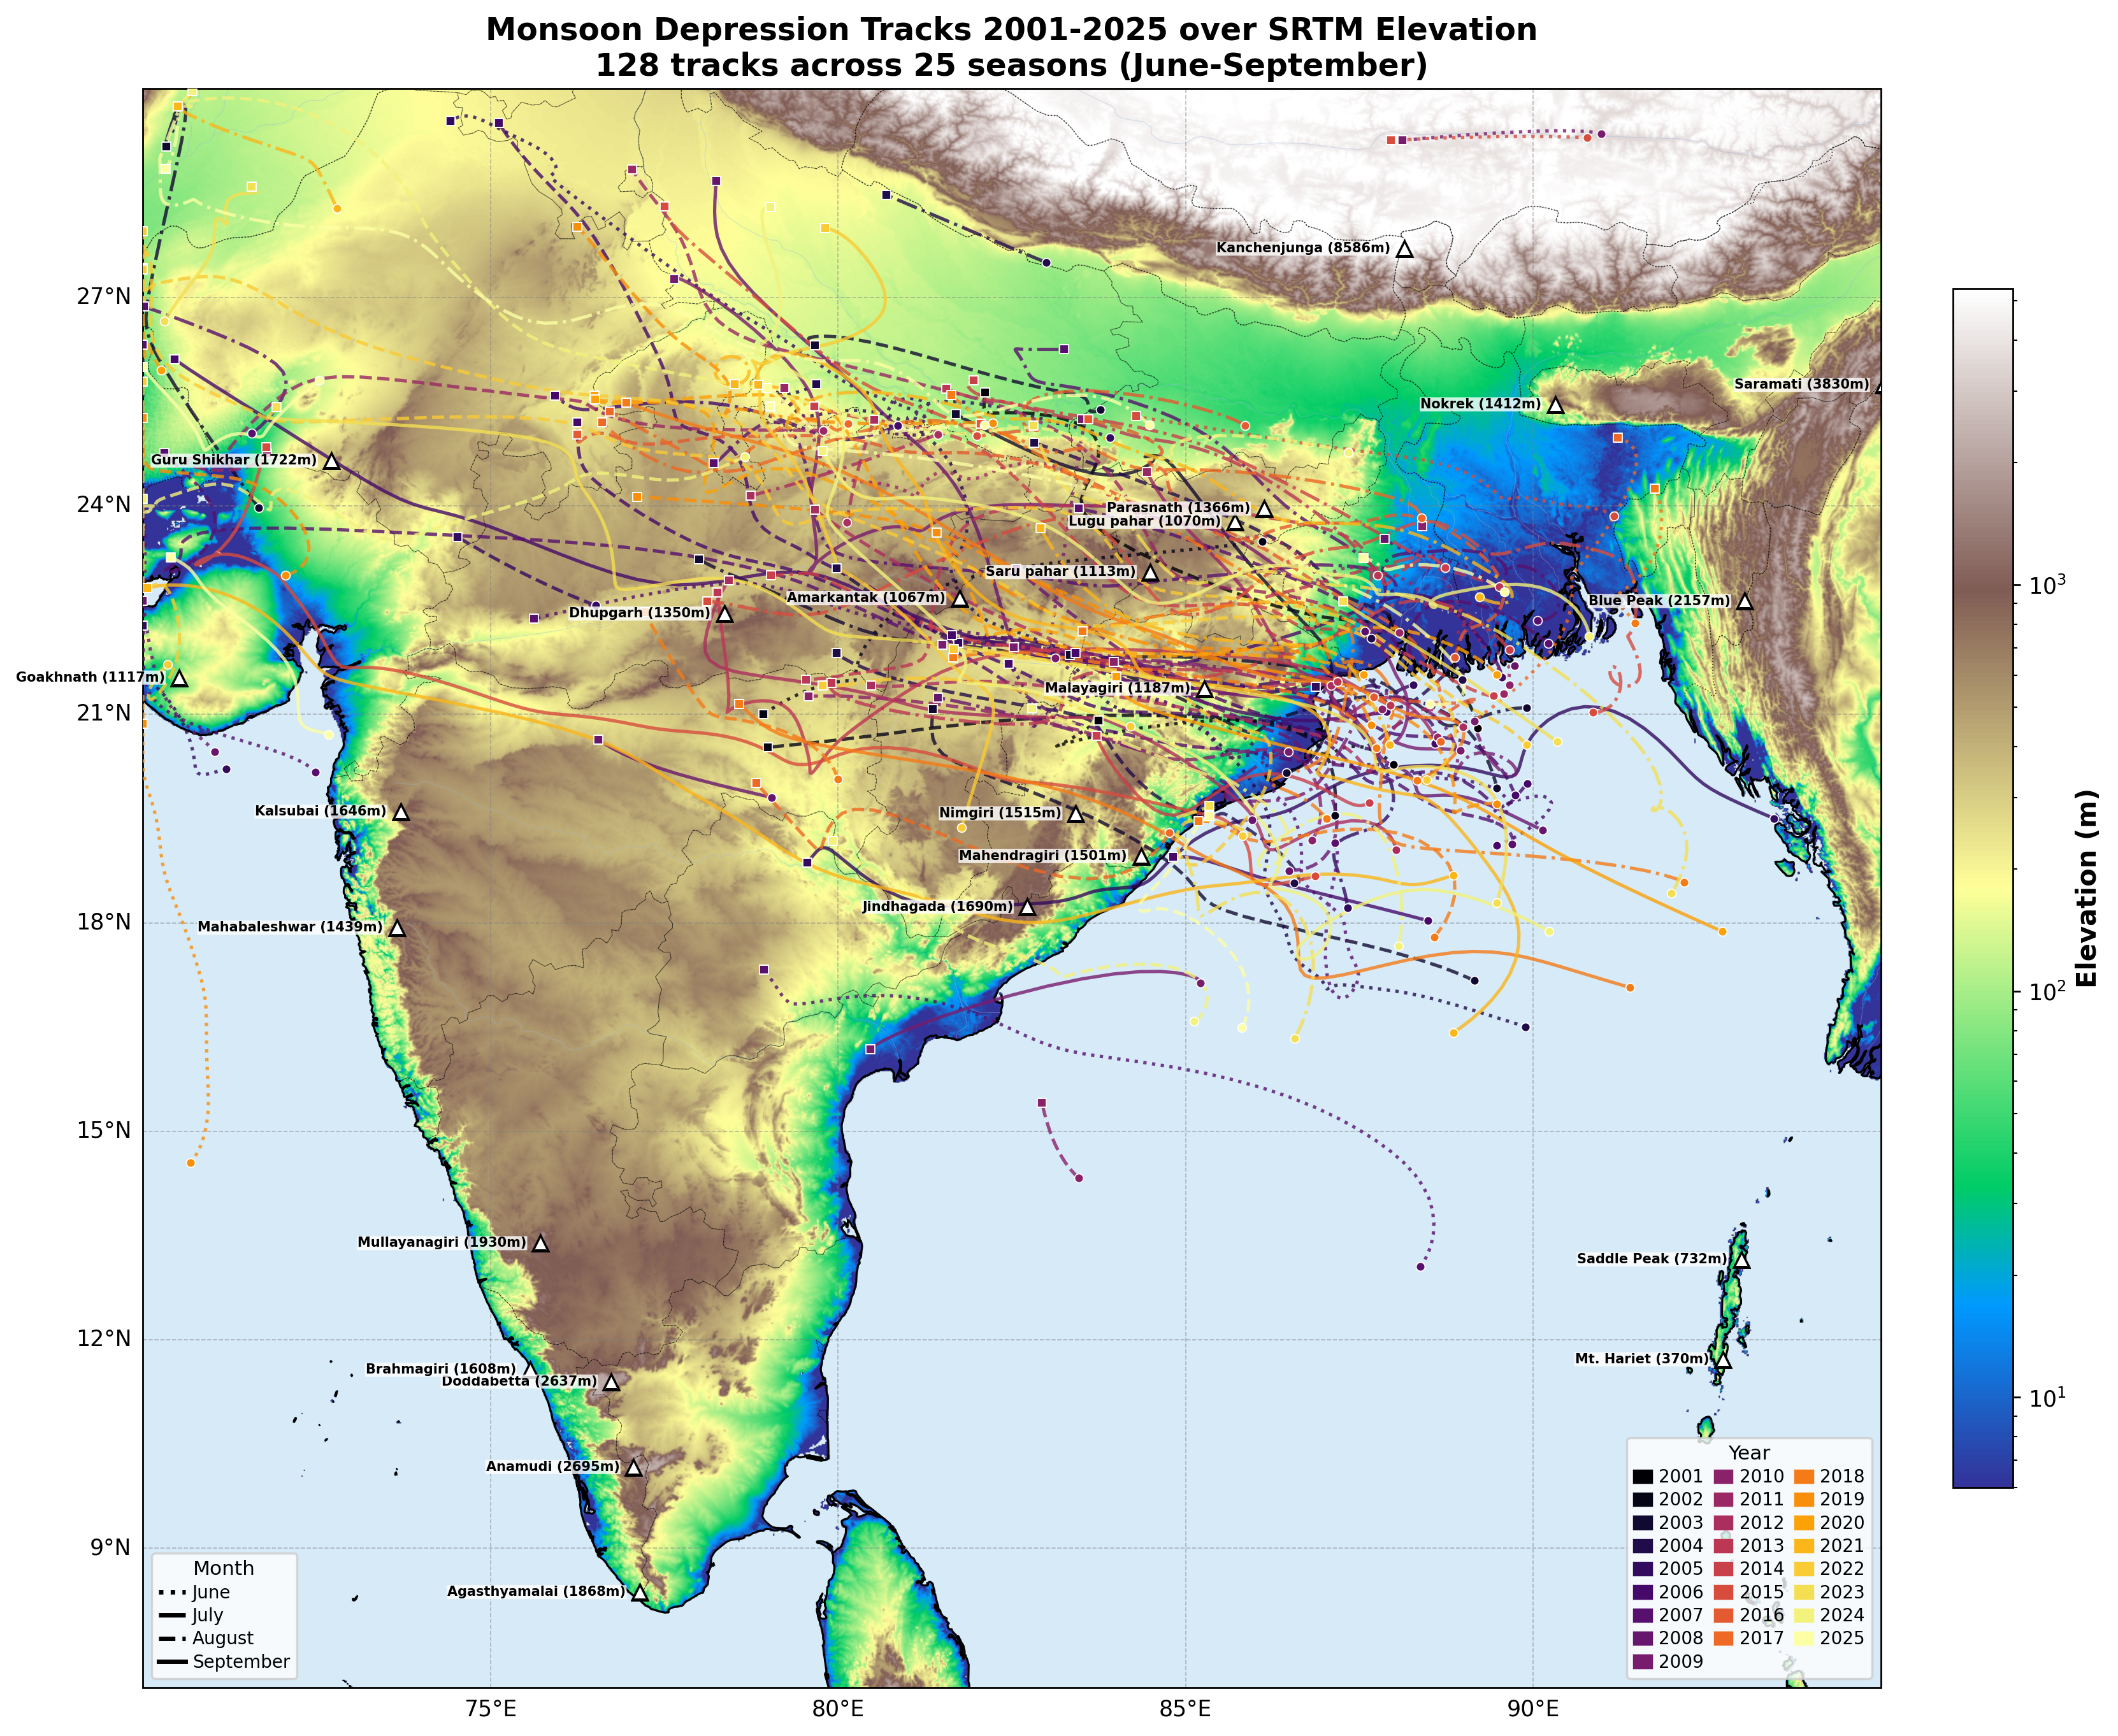
\includegraphics[width=0.78\textwidth]{all_years_tracks_elevation.png}
  \caption[Terrain elevation map of the Eastern Ghats and MD landfall
  zone]{All MD tracks from ERA5 (2001-2025). Colours and line style
    represents duration (year and months respectively) and contours
    represents elevation from SRTM. SRTM digital elevation model (m) of
  the Eastern Ghats and the eastern Deccan Plateau.}
  % The discontinuous ridge at 600-1000\,m is interrupted by the
  % Mahanadi (north), Godavari (south), and Brahmani river-valley gaps.
  % MD landfall tracks typically traverse the range within 24-48
  % hours of crossing the coast.}
  \label{fig:eastern_ghats_map}
\end{figure}
\vspace{-0.8cm}
\begin{figure}[H]
  \centering
  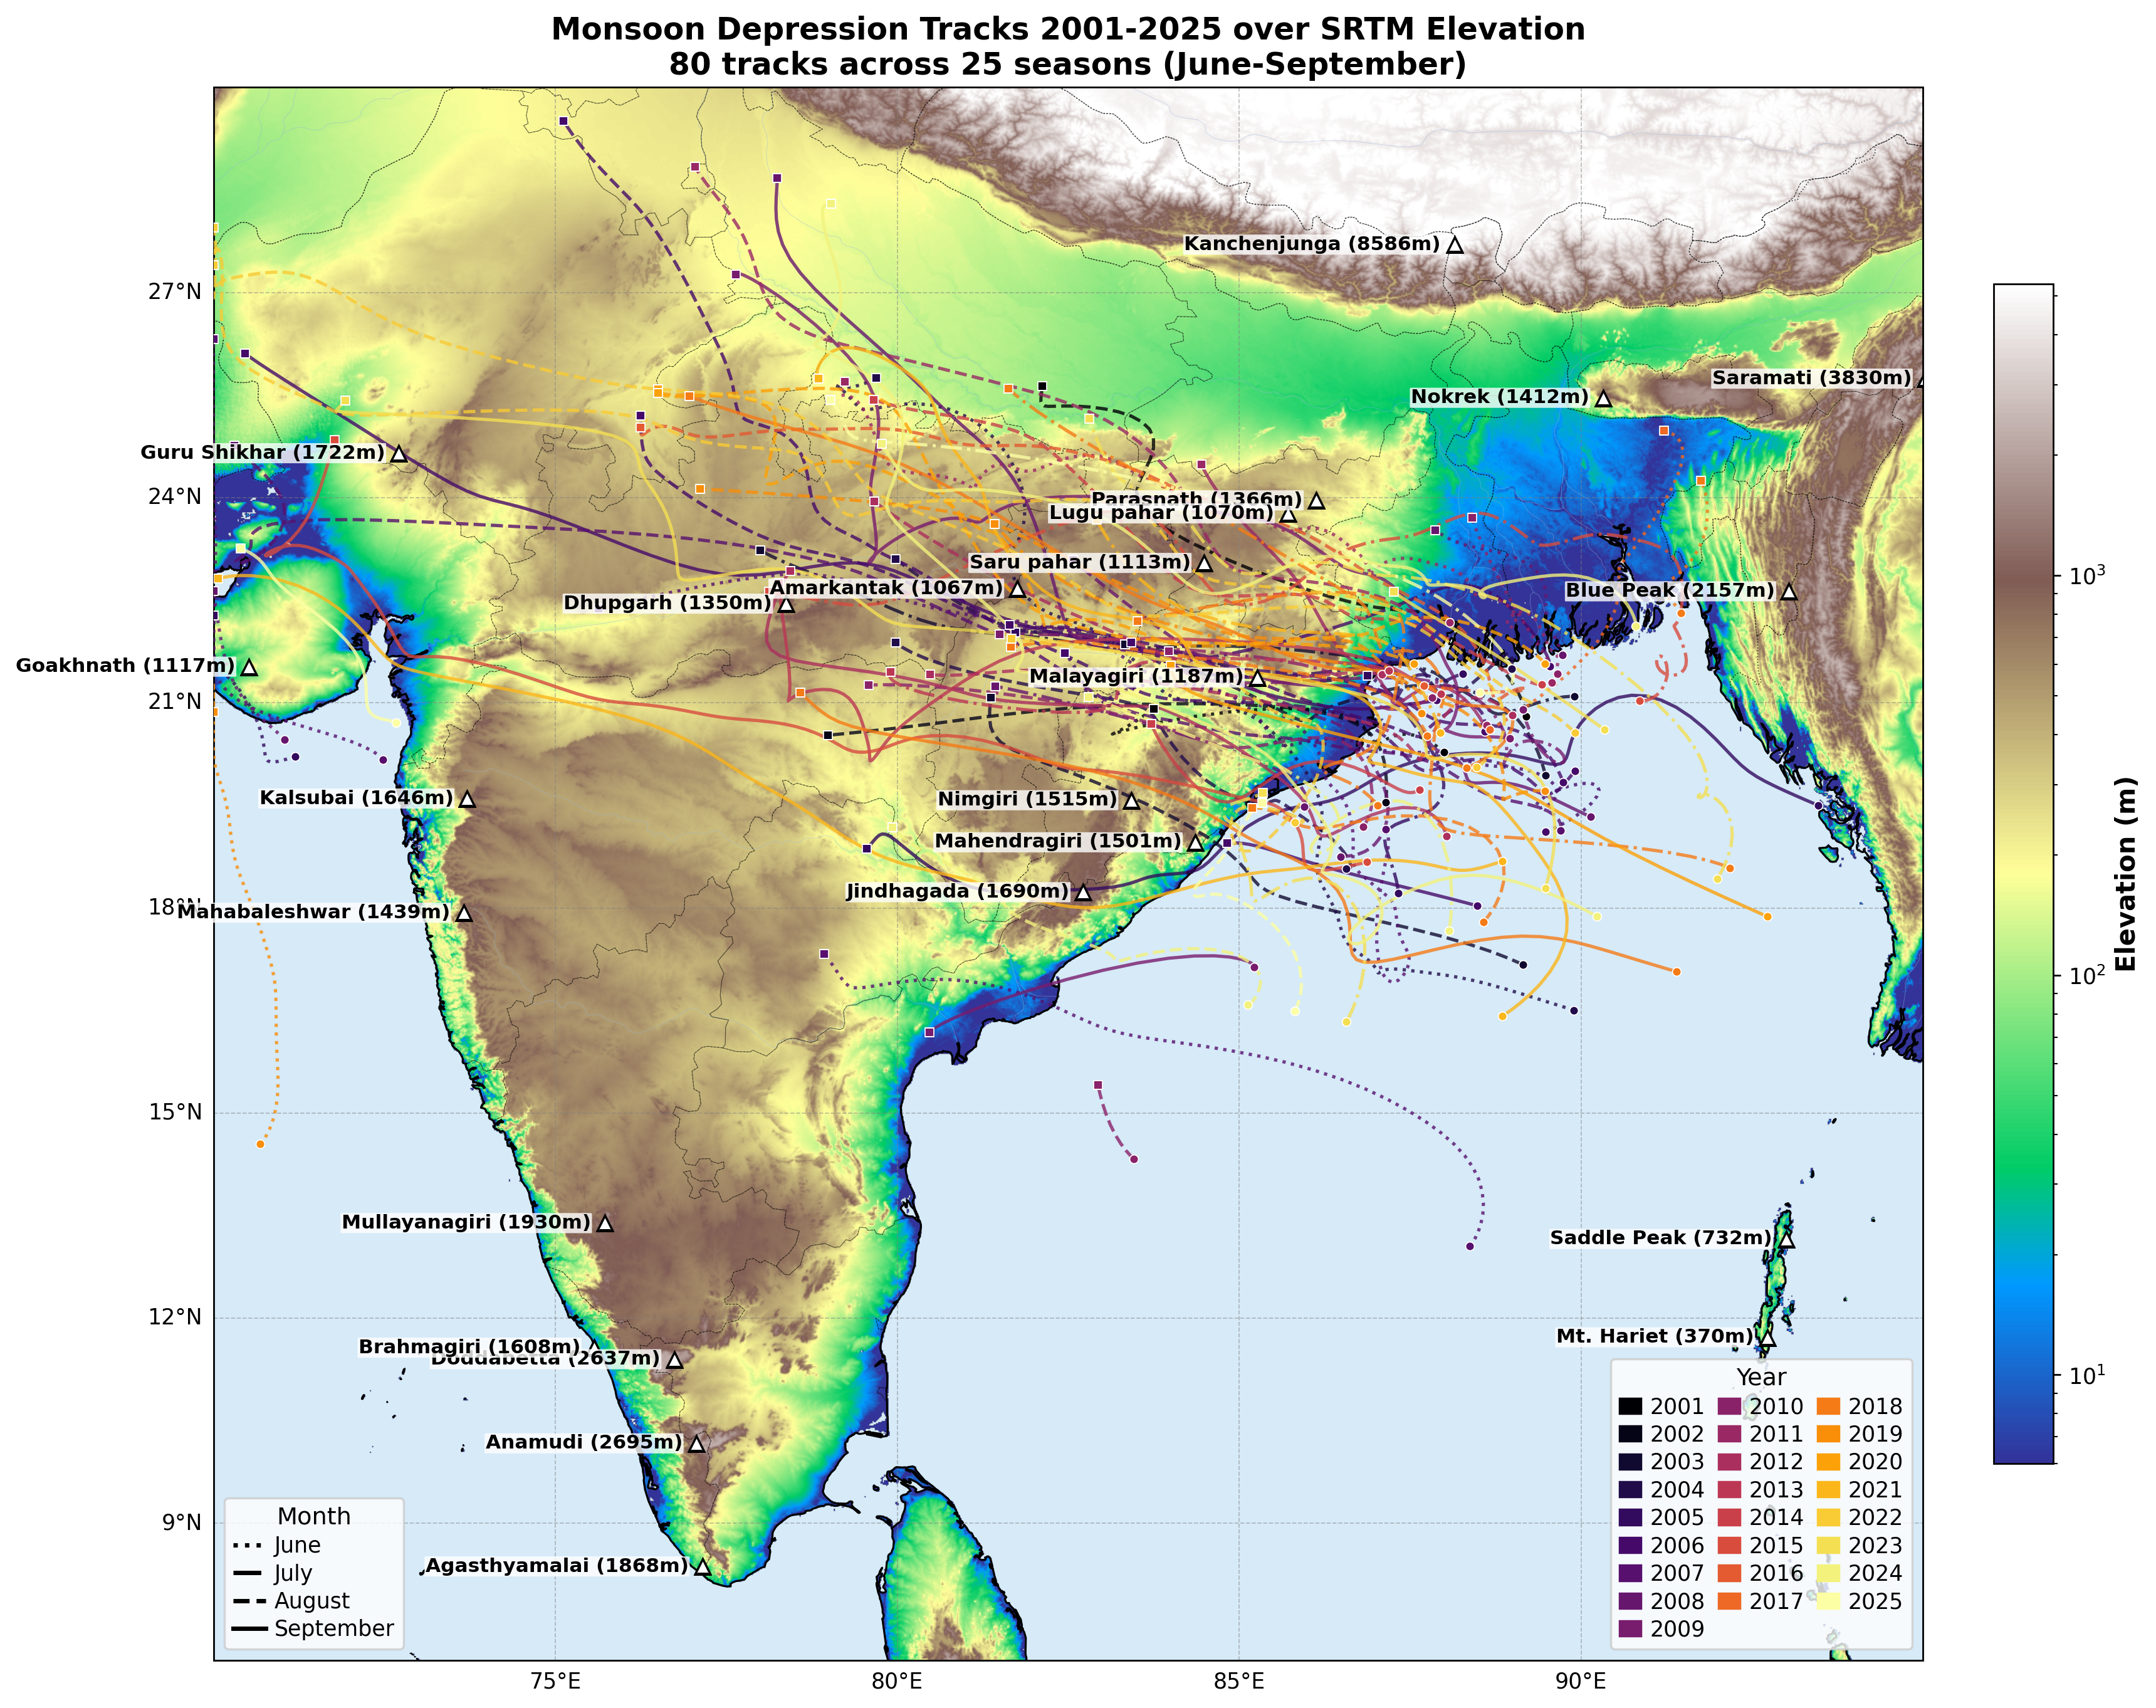
\includegraphics[width=0.78\textwidth]{ocean_only_tracks.png}
  \caption[Monsoon Depression track climatology of Ocean
  organinateMDs, 2001-2025]{Ocean organised MD tracks from ERA5
    (2001-2025). Colours and line style represents duration (year and
  months respectively) and contours represents elevation from SRTM.}
  \label{fig:ocean_md_tracks}
\end{figure}

\subsection{Four Mechanisms by Which the Eastern Ghats Block or Weaken MDs}
\label{subsec:ghats_mechanisms}

When an MD crosses the Eastern Ghats, four simultaneous physical
processes engage.

Together, these constitute the orographic modulation mechanism that
this thesis identifies as a major determinant of post-landfall fate:

\begin{enumerate}
  \item \textbf{Mechanism 1: Orographic precipitation enhancement and
    moisture removal.} Forced ascent on the windward (eastern)
    face of the Ghats  triggers orographic convection, substantially
    enhancing precipitation rates on the eastern slopes
    \autocite{houze1994, orographyconvection2005, medina2003analysis}.
    For a saturated, convectively unstable air column such as that
    within an MD, even modest forced ascent of 10-20\,cm\,s$^{-1}$
    over the 600-1000\,m terrain can release latent heat equivalent
    to deep convection. While this enhancement temporarily
    intensifies the MD's apparent rainfall on its eastern flank, it
    is simultaneously removing moisture from the inflowing
    boundary-layer air before it reaches the inner vortex. The result
    is that the MD's moisture budget is \emph{depleted} faster on the
    windward side than over the flat coastline, reducing the moisture
    available to sustain inner-core convection on the leeward side.
  \item \textbf{Mechanism 2: Translational speed deceleration.} As
    the MD crosses the terrain, increased surface roughness and the
    mechanical blocking effect of the elevated range decelerate the
    system's forward motion.
    % This deceleration is quantified in this study through the
    % Terrain Sensitivity Index (TSI).
    The deceleration has two consequences: (i) the MD spends more
    time over the windward slope, leading to extreme localised
    rainfall enhancement on the eastern Ghats face; and (ii) the
    low-level center stalls relative to the upper-level flow, forcing
    an increase in vortex tilt (Mechanism 4).
    % In some cases, MDs can become quasi-stationary over the Ghats for
    % hours before either crossing or dissipating. The degree of
    % blocking can be quantified through the \emph{Froude number}
    % approach \autocite{houze1994}:
    % \begin{equation}
    %   Fr = \frac{U}{Nh},
    %   \label{eq:froude}
    % \end{equation}
    % where $U$ is the approaching flow speed (MD translation speed,
    % $\approx 3$-5\,m\,s$^{-1}$), $N$ is the Brunt-Vaisala frequency
    % of the impinging air column, and $h$ is the terrain height
    % (600-1000\,m for the Eastern Ghats). When $Fr < 1$, the flow
    % tends to deflect around the barrier (blocking regime); when $Fr >
    % 1$, it can flow over the terrain. For typical MD conditions ($N
    % \approx 0.01$\,s$^{-1}$, $h = 800$\,m), $Fr \approx 0.4$-0.6,
    % placing MDs squarely in the partially-blocked regime, consistent
    % with observed speed reduction but not complete stoppage.
  \item \textbf{Mechanism 3: Low-level easterly moisture inflow
    blocking.} The most consequential effect of the Eastern Ghats on
    MD energetics is the blockage of the low-level easterly moisture
    inflow from the BoB. Pre-landfall, the MD draws a continuous
    supply of warm, moisture-laden air from the Bay of Bengal through
    its eastern sector (the inflow region), sustaining the water
    vapour mixing ratio in the inner core. As the terrain obstructs
    this inflow, the Integrated Vapour Transport (IVT) from the BoB
    peaks around at 300K drops sharply (Figure~\ref{fig:ivt_example}).
    On the leeward side, the MD must draw on local surface
    evapotranspiration (if BOE-active) or face rapidly declining
    moisture availability in its inner core.
    The transition from \emph{oceanic} moisture inflow to \emph{local
    surface} moisture supply at the terrain crossing is the fundamental
    energy-source switch this thesis documents.
  \item \textbf{Mechanism 4: Vortex Tilt and Structural Decoupling.}
    The Eastern Ghats selectively slow the low-level (850\,hPa) MD
    center while the upper-level (200-300\,hPa) anticyclonic outflow,
    being largely unaffected by surface terrain, continues to
    propagate westward at the large-scale steering speed. The result
    is an increasing westward displacement of the upper warm core
    relative to the low-level vortex-an increasing vortex tilt
    (Section~\ref{subsec:vortex_tilt_background}). When the tilt
    exceeds the critical threshold, the latent heat release in the
    convective updrafts no longer efficiently maintains the warm core
    above the surface convergence zone, and the vortex loses vertical
    coherence. This is the structural mechanism of terrain-induced
    weakening. The Vortex Tilt analysis directly measures this
    evolution (Figure~\ref{fig:vortext_tilt}).
\end{enumerate}

% \begin{figure}[H]
%   \centering
%   %% Note: DRAW THIS FIGURE - cross-section schematic showing:
%   %%   Left (east): BoB, MD circulation, easterly moisture inflow arrows
%   %%   center: Eastern Ghats (600-1000m hill profile)
%   %%   Windward side: forced ascent, orographic rain enhancement (raindrops)
%   %%   Leeward side: descending dry air (foehn), vortex tilt arrow
%   %%   Upper arrows: upper-level flow continuing westward faster
% than low-level
%   %%   Label: "Low-level center stalls", "Upper warm core advances",
%   % "IVT blocked"
%   \fbox{\rule{0pt}{7cm}\rule{0.90\textwidth}{0pt}}
%   % \includegraphics[width=0.90\textwidth]{ghats_blocking_schematic}
%   \caption[Schematic of Eastern Ghats orographic modulation of a
%   landfalling MD]{East-west cross-section showing the four mechanisms
%     by which the Eastern Ghats modulate a landfalling MD. (1)
%     Orographic precipitation enhancement on the windward face depletes
%     the moisture column. (2) Frictional deceleration stalls the
%     low-level center. (3) Low-level easterly BoB moisture inflow is
%     blocked by the terrain. (4) The upper-level warm core continues
%     westward faster than the surface low, increasing vortex tilt.
%     BOE-candidate systems counteract mechanisms 3 and 4 through
%   sustained surface LHF on the leeward side.}
%   \label{fig:ghats_blocking_schematic}
% \end{figure}
\begin{figure}[H]
  \centering
  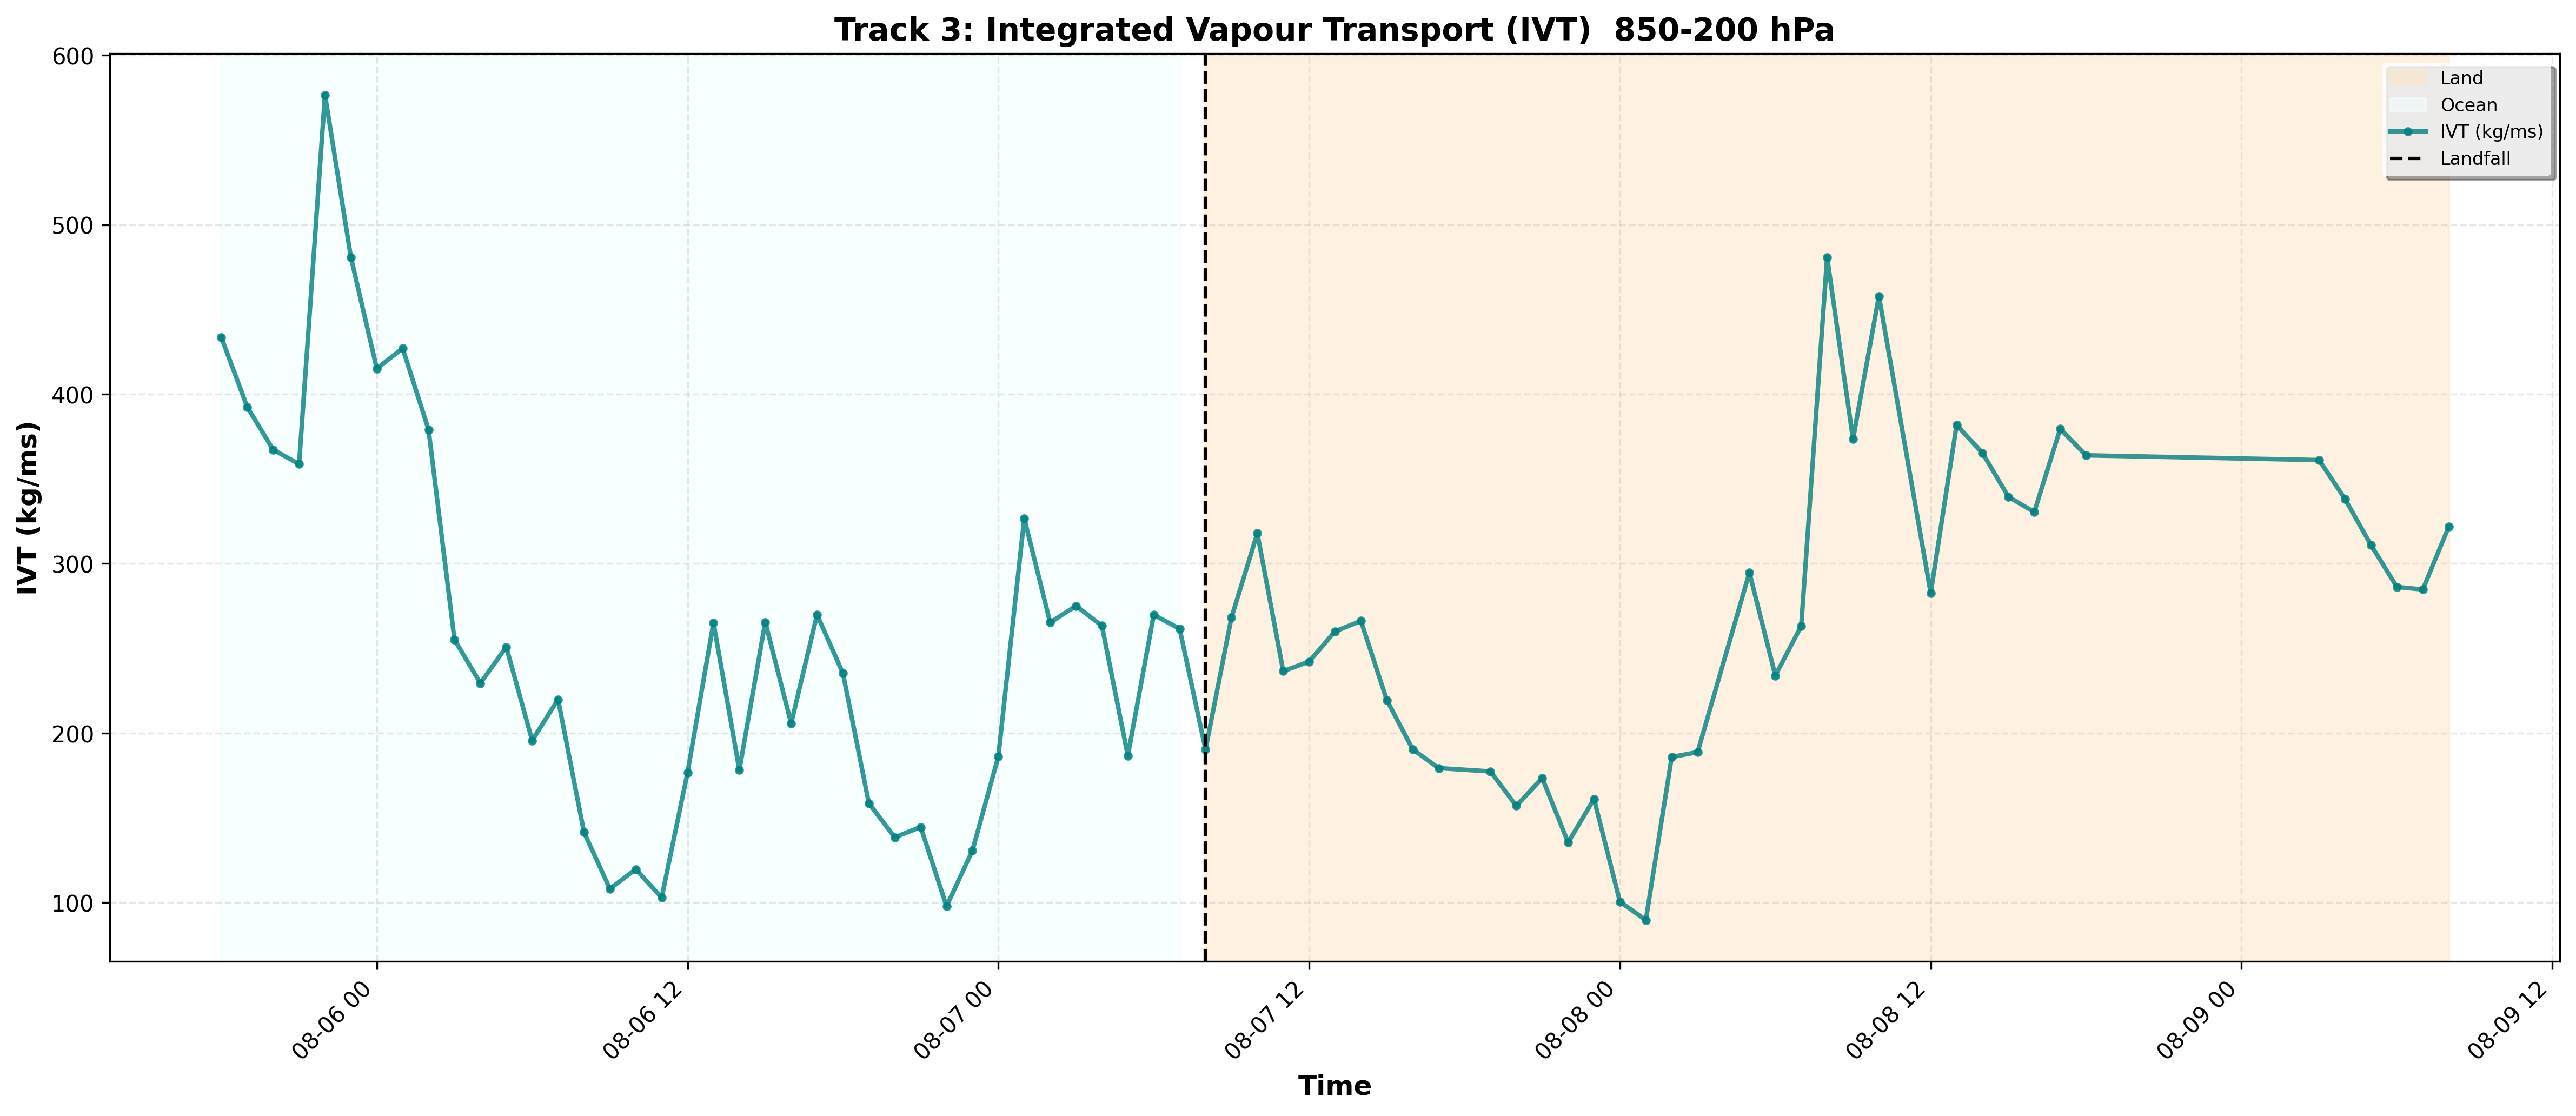
\includegraphics[width=0.95\textwidth]{ivt_example}
  \caption{Integrated Vapour Transport (IVT) analysis showing the
    sharp increase then drop in moisture flux from the Bay of Bengal as the MD
  encounters land.}
  \label{fig:ivt_example}
\end{figure}

\begin{figure}[H]
  \centering
  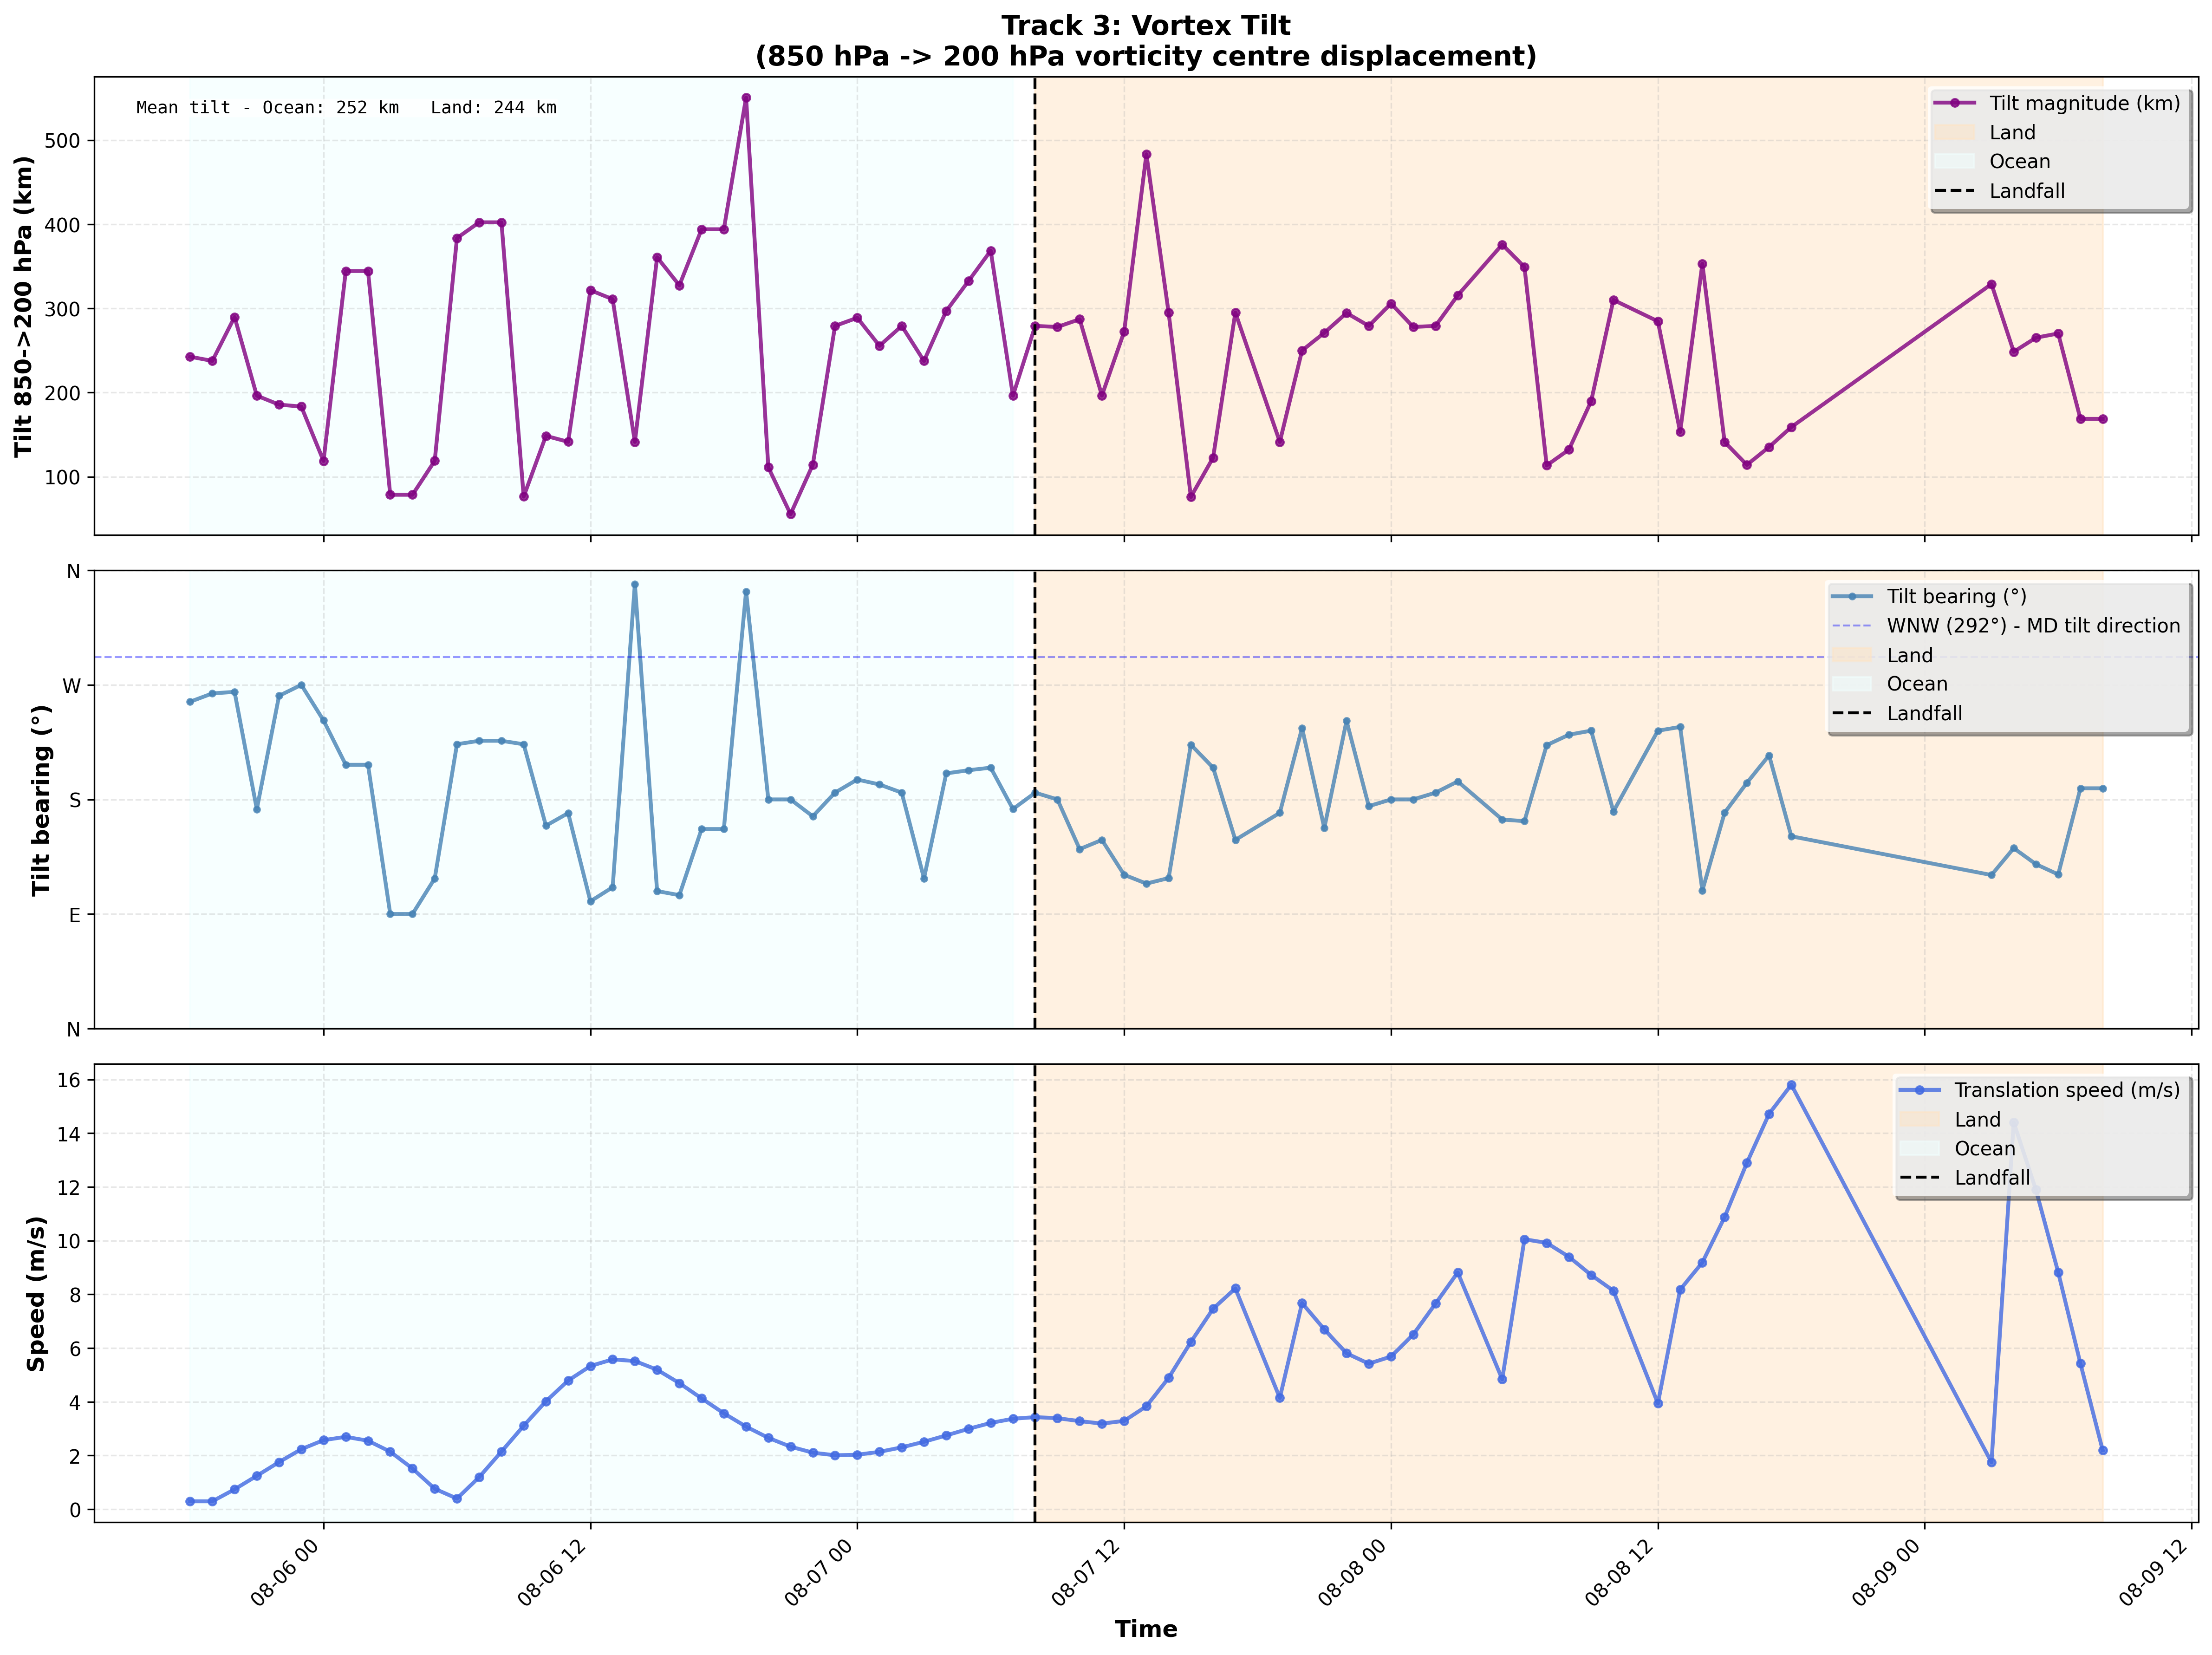
\includegraphics[width=0.95\textwidth]{vortex_tilt_example}
  \caption{Evolution of vortex tilt during terrain crossing,
    illustrating the structure between the low-level center and the
  upper-level warm core.}
  \label{fig:vortext_tilt}
\end{figure}

\subsection{The BOE as a Counter-Mechanism to Ghats-Induced Decay}
\label{subsec:boe_ghats_interaction}

The interaction between the Eastern Ghats blocking mechanisms
(Section~\ref{subsec:ghats_mechanisms})
and the Brown Ocean Effect is the central scientific question of this
research and its primary finding. The four decay mechanisms described
above are simultaneously counteracted by BOE surface LHF through the
following physical pathways:
\begin{enumerate}
  \item \emph{Against Mechanism 3 (moisture inflow blocking):} The
    BOE replaces the lost BoB moisture inflow with locally sourced
    evapotranspiration. While the mixing ratio of locally evaporated
    soil moisture is not identical to the warm, deep BoB moisture
    column (which extends to 500\,hPa), it is sufficient to maintain
    near-surface specific humidity and CAPE in the inner-core
    boundary layer above the BOE threshold. The key diagnostic is the
    leeward-sector dew-point depression (DPD): a BOE candidate system
    shows smaller leeward DPD increase during terrain crossing
    because surface evapotranspiration.% actively counteracts the
    % föhn-induced drying.
  \item \emph{Against Mechanism 4 (vortex tilt):} Sustained LHF at
    the land surface maintains low-level boundary-layer convergence
    (driven by the moist instability above the high-LHF zone),
    effectively keeping the surface pressure gradient alive beneath
    the stalling low-level center. This ``anchors'' the low-level
    center and limits tilt growth. A system with sustained BOE LHF
    should therefore show tilt stabilisation on the leeward side; a
    non-BOE system shows monotonically increasing tilt leading to
    structural collapse. \\
    Comparison of vortex tilt evolution between BOE-active and
    non-BOE systems. Figure~\ref{fig:boe_tilt_comparison} shows how
    sustained surface LHF anchors the low-level center, limiting tilt
    growth. The Figure~\ref{fig:non_boe_tilt_comparison} illustrates
    highly varying and increasing tilt leading to decoupling in the
    absence of surface moisture flux.
    \begin{figure}[H]
      \centering
      % --- BOE Stability ---
      \begin{subfigure}[b]{0.49\textwidth}
        \centering
        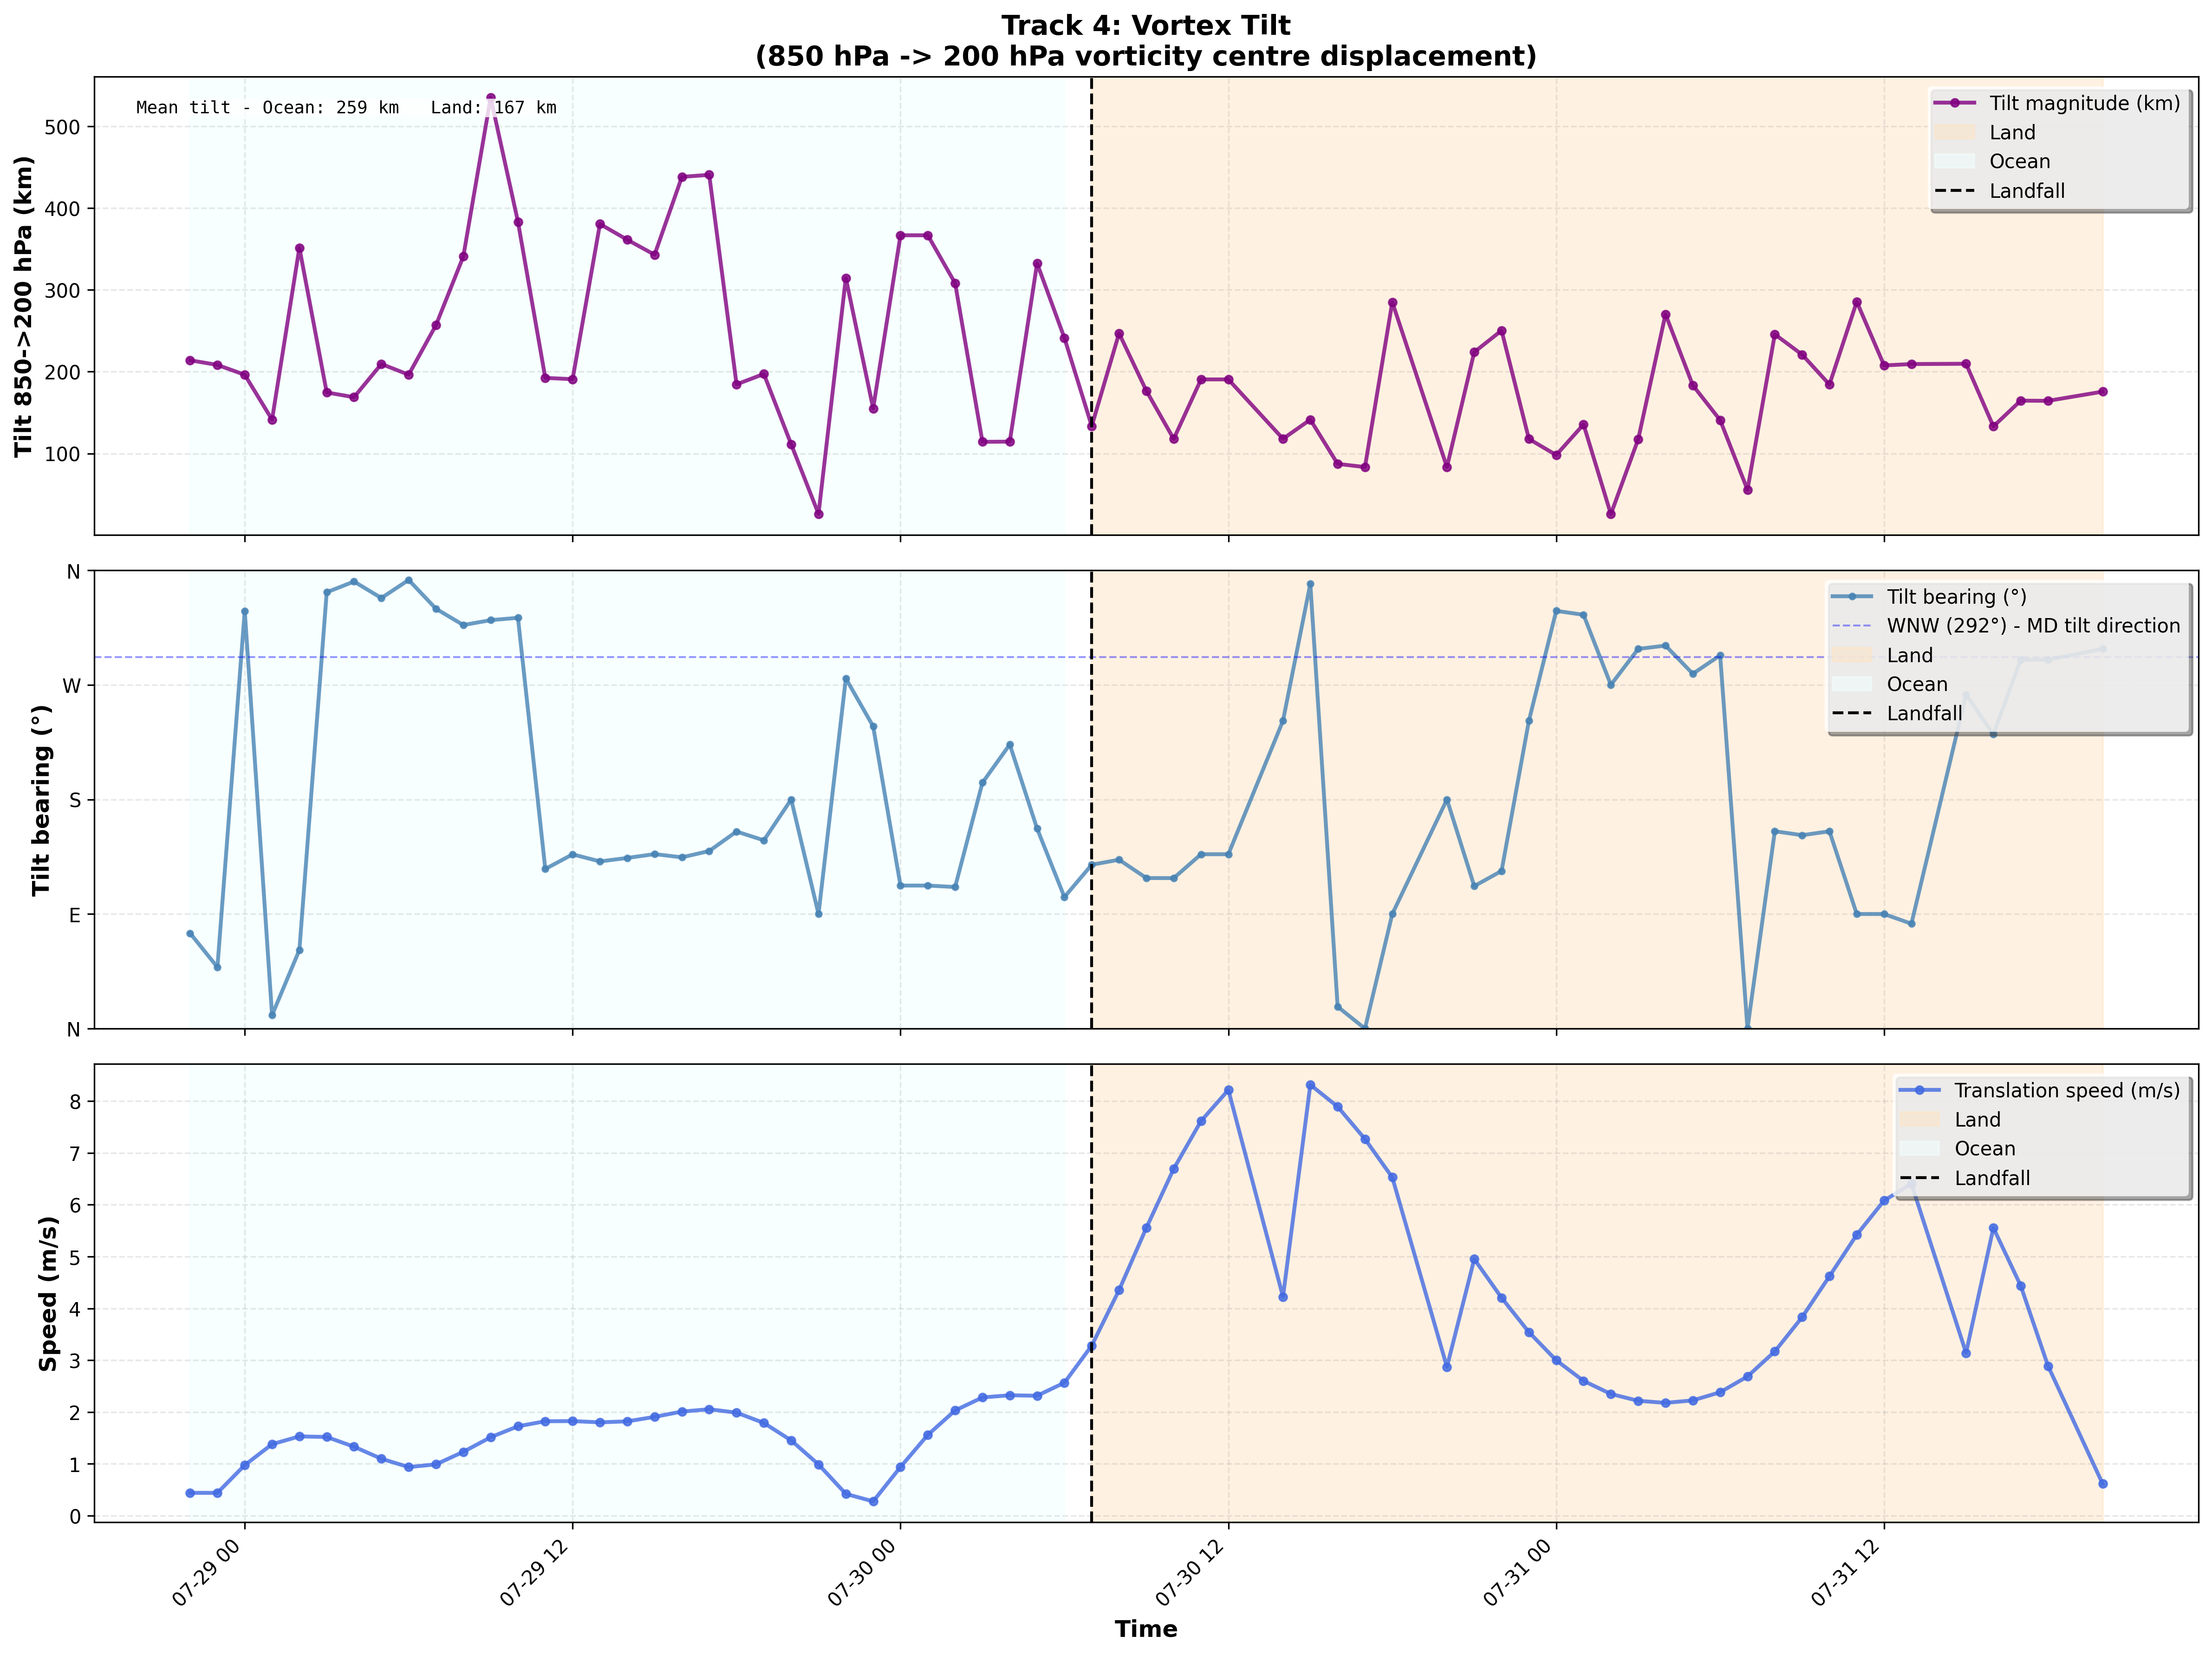
\includegraphics[width=\textwidth]{boe_tile_stabilisation_1.png}
      \end{subfigure}
      \hfill
      \begin{subfigure}[b]{0.49\textwidth}
        \centering
        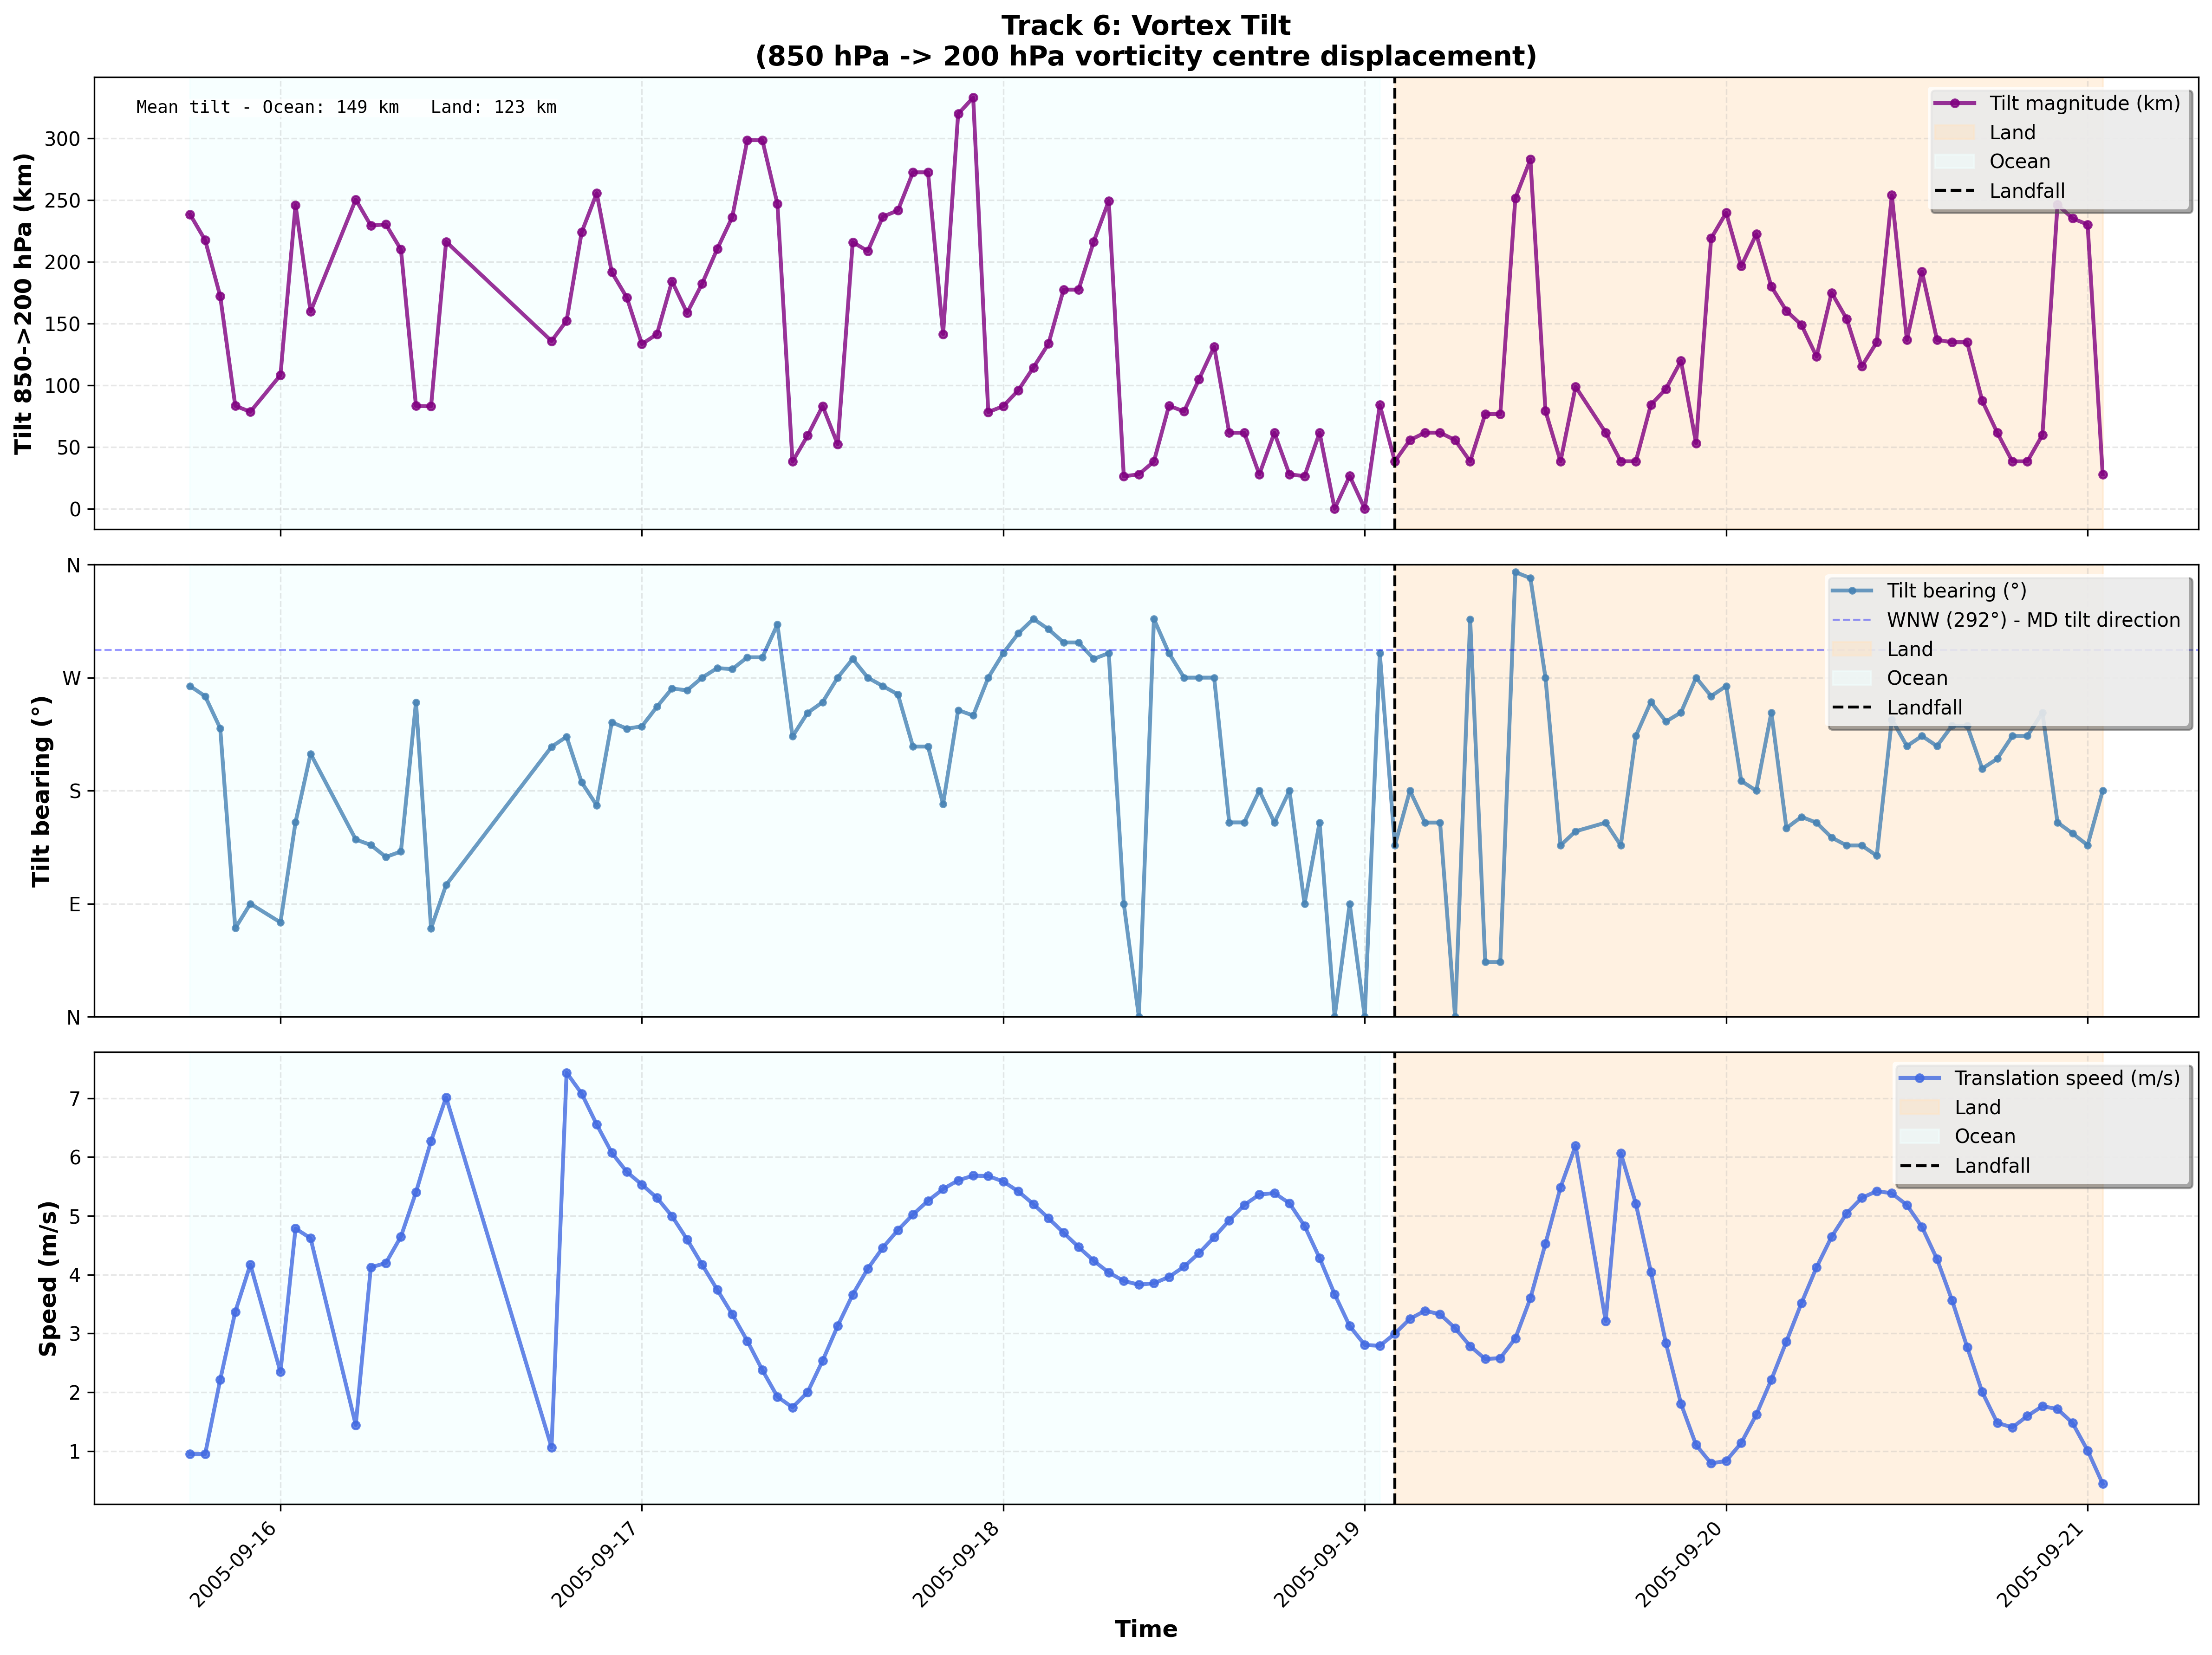
\includegraphics[width=\textwidth]{boe_tile_stabilisation_2.png}
      \end{subfigure}
      \caption{BOE Case: Initial crossing and Tilt stabilization}
      \label{fig:boe_tilt_comparison}
    \end{figure}
    \vspace{-0.5cm}
    \begin{figure}[H]
      % --- Non-BOE Astability ---
      \begin{subfigure}[b]{0.49\textwidth}
        \centering
        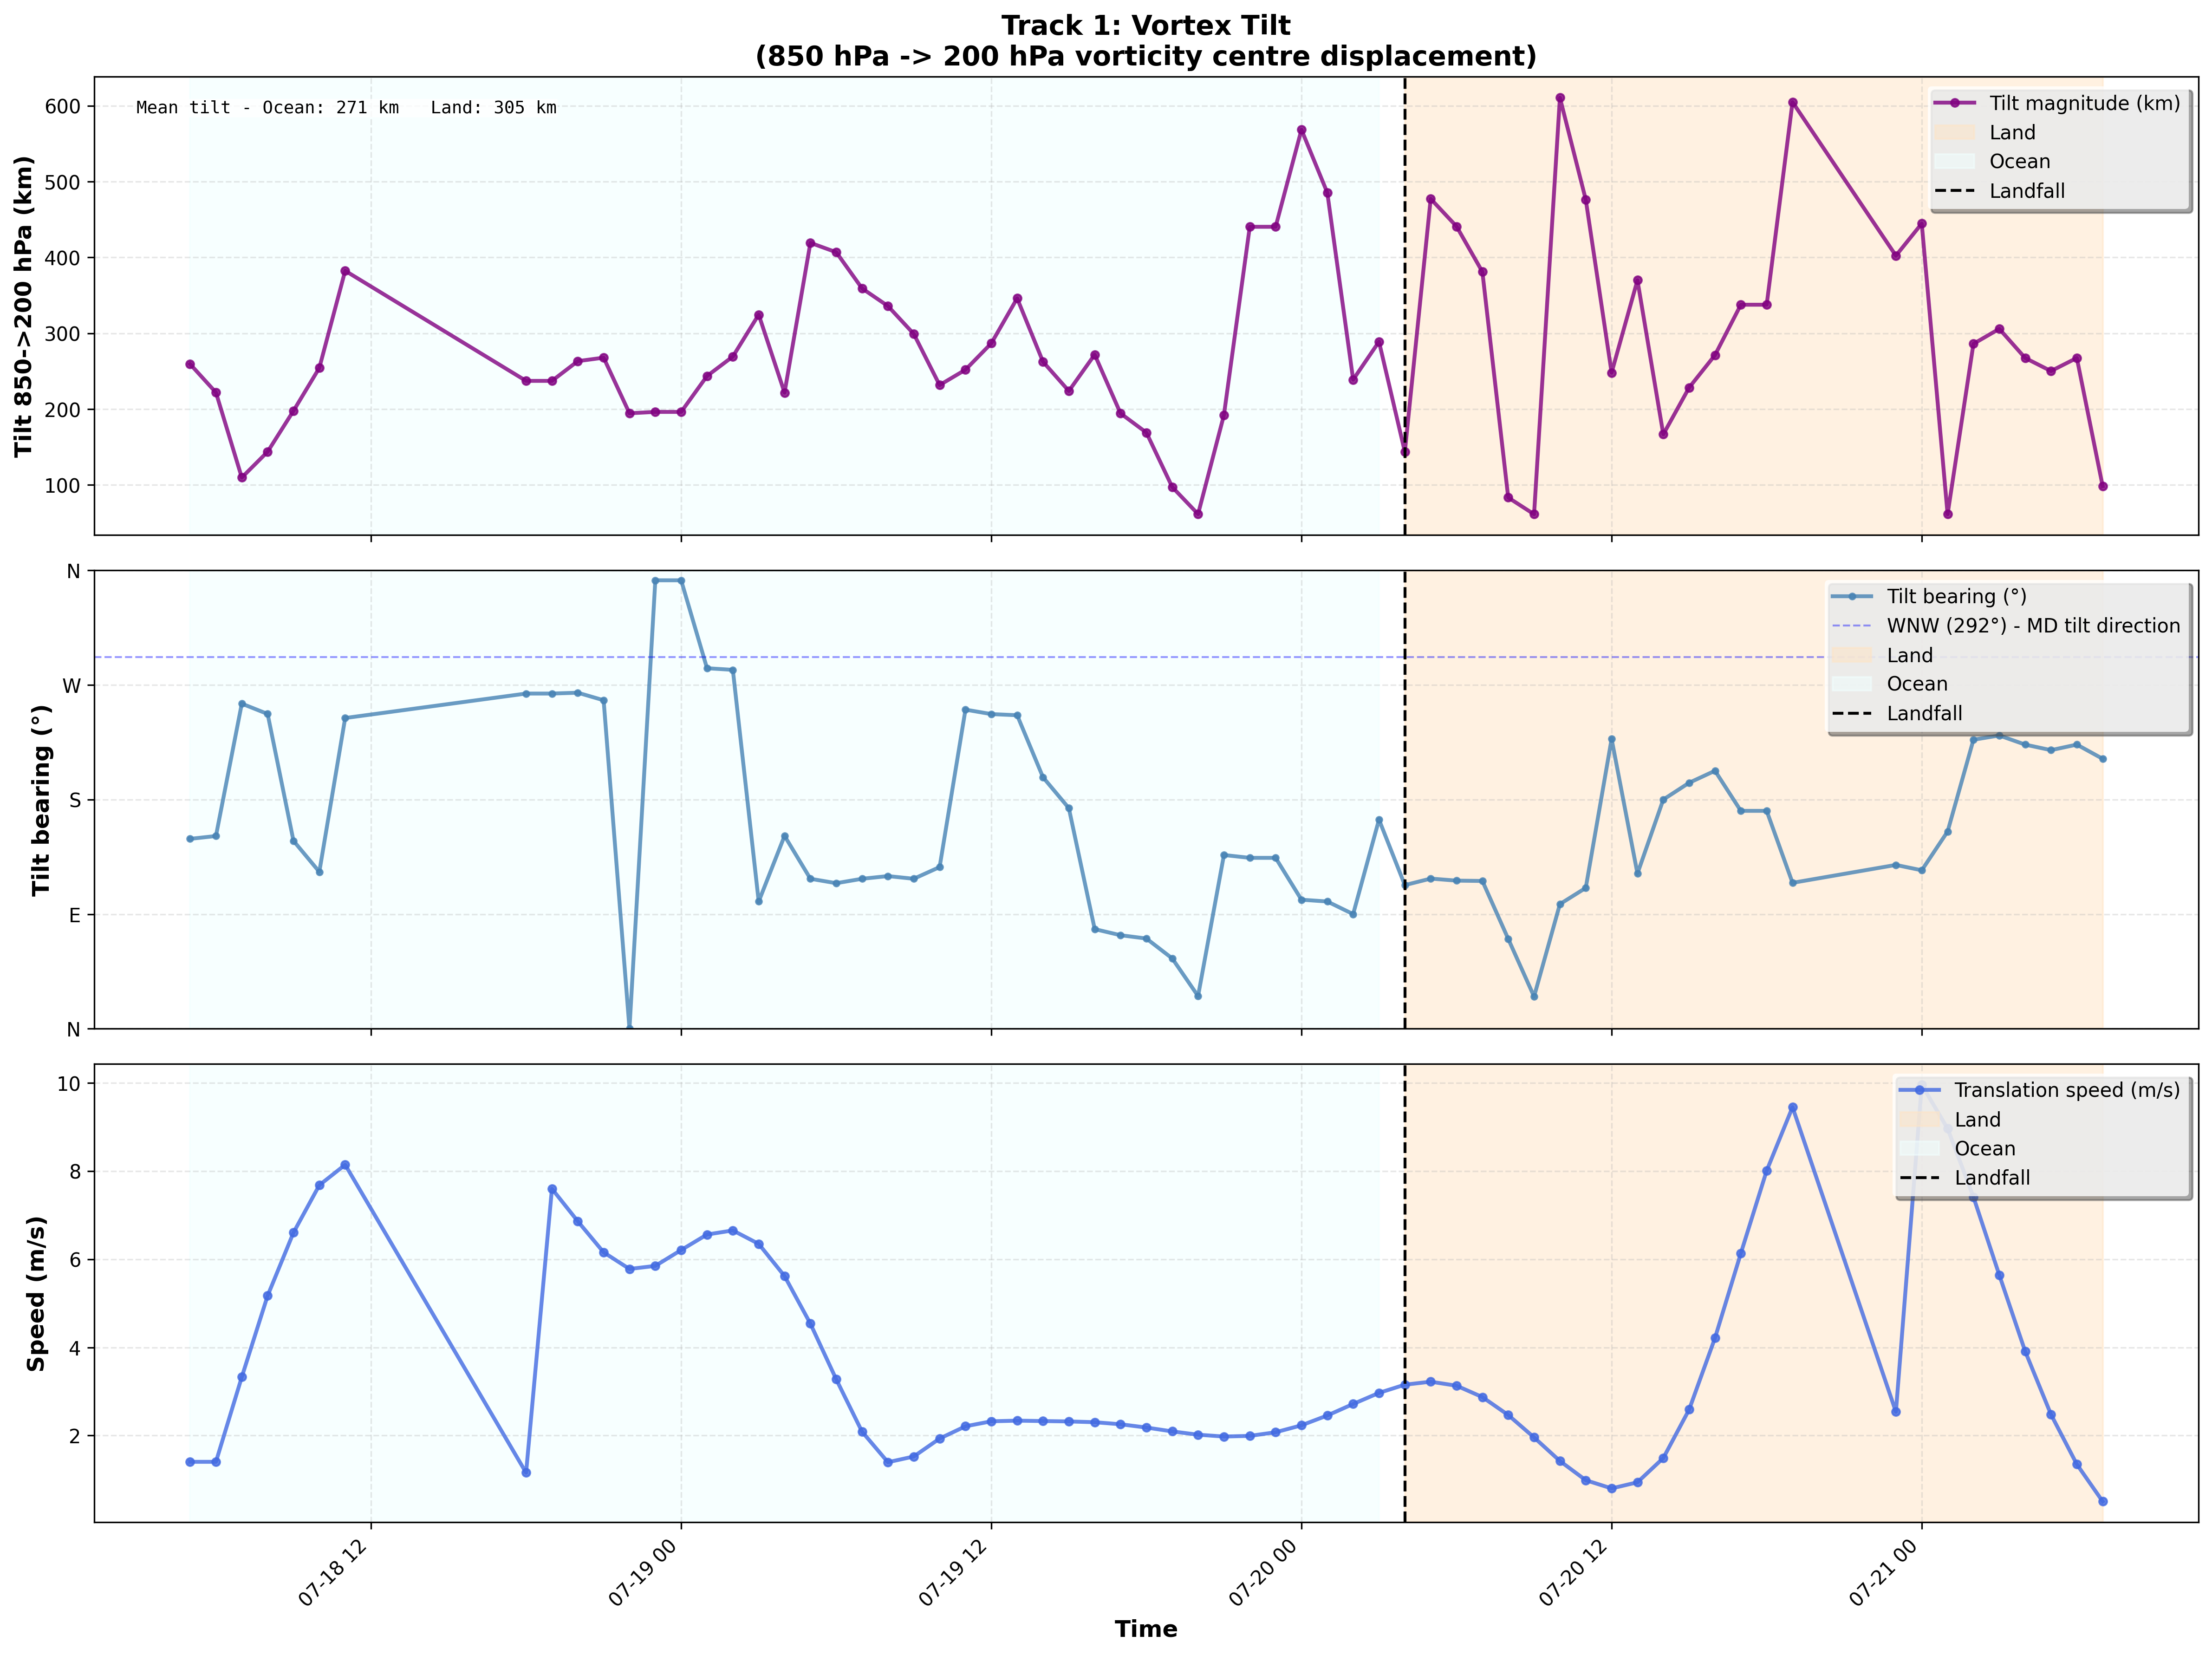
\includegraphics[width=\textwidth]{non_boe_tile_astabilisation_1.png}
      \end{subfigure}
      \hfill
      \begin{subfigure}[b]{0.49\textwidth}
        \centering
        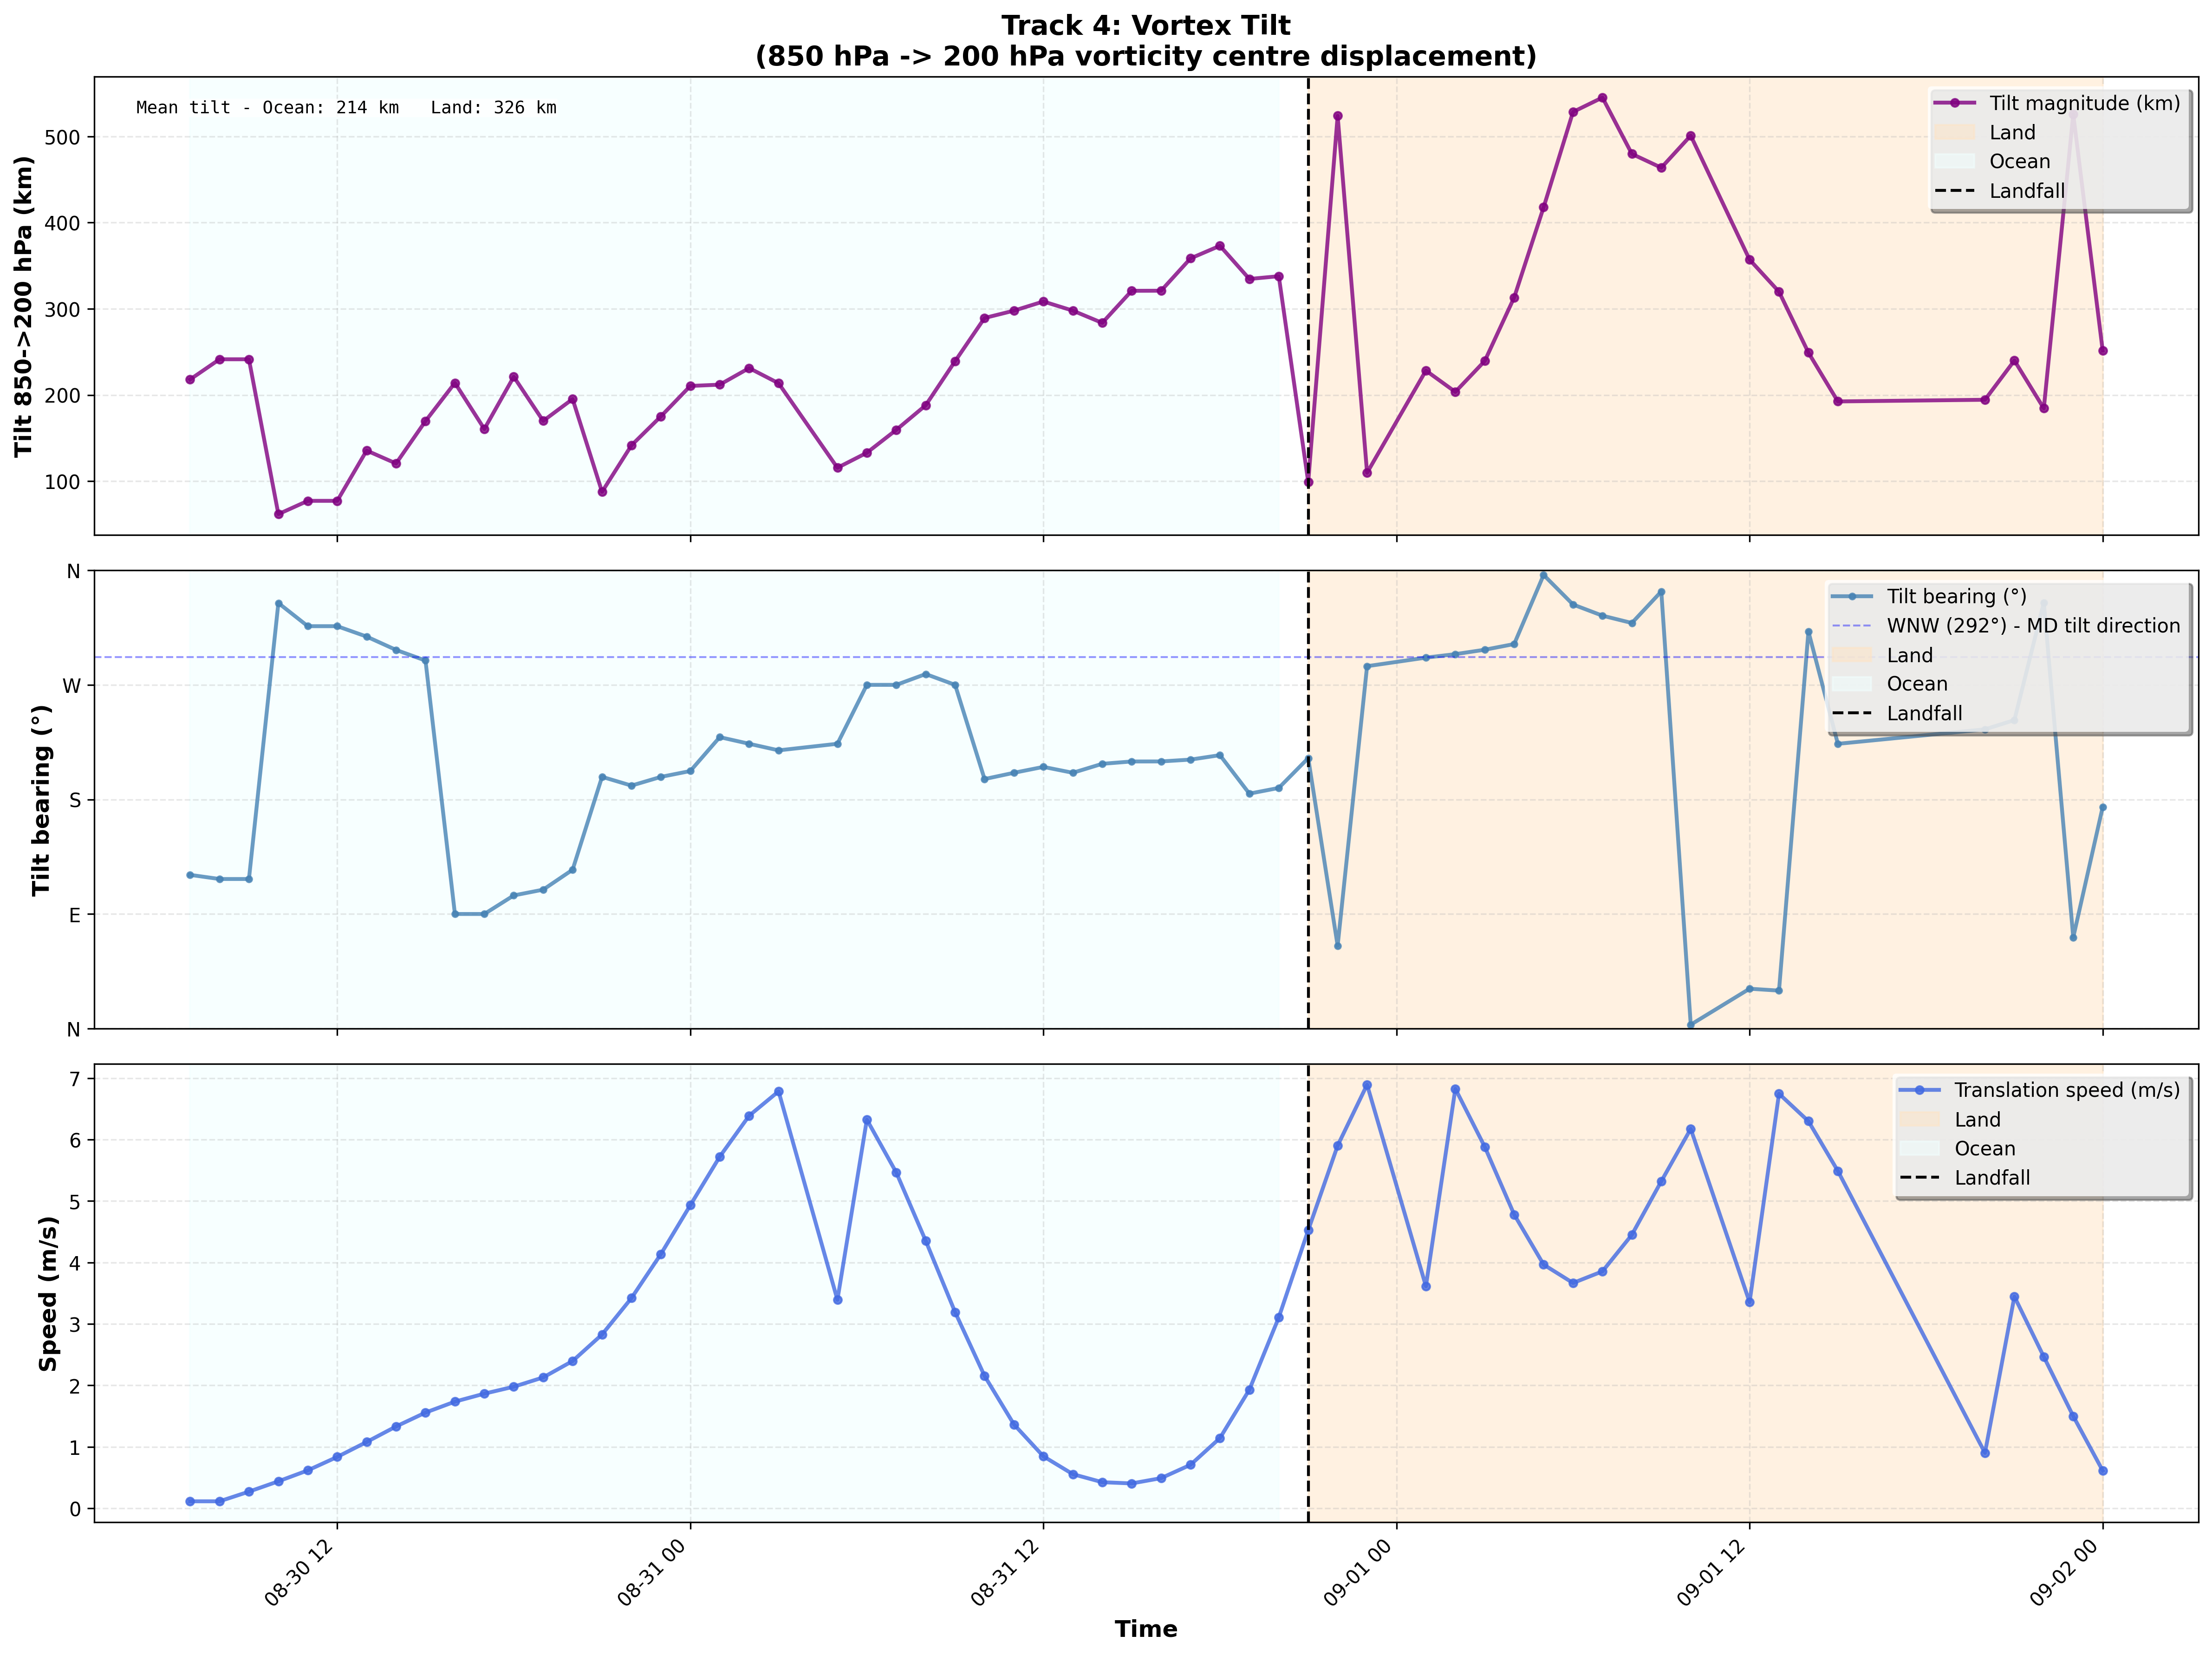
\includegraphics[width=\textwidth]{non_boe_tile_astabilisation_2.png}
      \end{subfigure}
      \caption{Non-BOE Case: Increasing tilt and Structural collapse}
      \label{fig:non_boe_tilt_comparison}
    \end{figure}
\end{enumerate}

The net result, confirmed by the translational speed recovery
analysis in this thesis, is that sufficiently pre-moistened surfaces
allow BOE candidates to \emph{pass through} the Eastern Ghats: they
decelerate in the terrain zone but re-accelerate on the leeward side.
This differential between BOE and non-BOE speed recovery is the
single most operationally significant finding of this study, as it
directly predicts whether a system will produce extended inland flooding.

% \yellownote{TODO: add subsection about ITCZ and it's role}
% \subsection{The Inter-Tropical Convergence Zone}
% The ITCZ marks the equatorial boundary between the northern and
% southern Hadley cells. During the NH summer it migrates to
% 5-10$^\circ$N over the Indian Ocean, providing the region of maximum
% low-level convergence into which the cross-equatorial Somali Jet
% flows. MDs forming near the BoB head are partly sustained by the
% convergent moisture flux associated with the ITCZ's northward
% migration - the same flux that the Findlater Jet intensifies and
% channels northward. The ITCZ position thus modulates both the
% moisture supply and the background vorticity available for MD genesis.
 %% Background and Literature Review
%%  Chapter 3 - Data and Methodology

\ifpdf
\graphicspath{{chapters/Figs/}{chapters/Figs/Raster/}{Figs/PDF/}{Figs/}}
\else
\graphicspath{{chapters/Figs/}{chapters/Figs/Vector/}{Figs/}}
\fi

\chapter{Data and Methodology}
\label{ch:methodology}

\section{Data Sources}
\label{sec:data_sources}

\subsection{ERA5 Reanalysis}
\label{subsec:era5}

The primary dataset is the ERA5 global reanalysis produced by the
European center for Medium-Range Weather Forecasts (ECMWF)
\autocite{hersbach2020era5}. ERA5 provides hourly estimates of
atmospheric, land-surface, and oceanic variables on a regular
latitude-longitude grid at $0.25^\circ \times 0.25^\circ$ horizontal
resolution (approximately 28\,km at the equator), with 37 pressure
levels from 1000\,hPa to 1\,hPa. The dataset is generated through a
4D-Var data assimilation system that ingests conventional and
satellite observations \autocite{hersbach2020era5}.

The following ERA5 surface and single-level fields are used at hourly
temporal resolution over the domain 5-35$^\circ$N, 60-100$^\circ$E:

\begin{itemize}
  \item \textbf{850\,hPa relative vorticity} (\texttt{vo}): MD
    detection, tracking, and center identification.
  \item \textbf{Mean sea-level pressure} (\texttt{msl}):
    closed-circulation verification.
  \item \textbf{Surface latent heat flux} (\texttt{slhf},
    J\,m$^{-2}$, accumulated): de-accumulated to W\,m$^{-2}$;
    positive upward throughout.
  \item \textbf{Surface sensible heat flux} (\texttt{sshf},
    J\,m$^{-2}$, accumulated): de-accumulated identically.
  \item \textbf{Volumetric soil water layer\,1} (\texttt{swvl1},
    m$^3$\,m$^{-3}$): 0-7\,cm near-surface soil moisture, instantaneous.
  \item \textbf{Total precipitation} (\texttt{tp}, m\,hr$^{-1}$,
    accumulated): de-accumulated to mm\,hr$^{-1}$.
  \item \textbf{2-m dewpoint temperature} (\texttt{d2m}, K):
    boundary-layer moisture saturation state.
  \item \textbf{2-m temperature} (\texttt{t2m}, K): surface thermodynamic state.
  \item \textbf{Land-sea mask} (\texttt{lsm}): land/ocean
    classification (\texttt{lsm} $\geq 0.5$ = land).
  \item \textbf{10-m U and V wind components} (\texttt{u} and
    \texttt{v}, ms$^{-1}$): translational flow environment.
\end{itemize}

ERA5 accumulated flux variables are de-accumulated to instantaneous values as:
\begin{equation}
  F_\mathrm{inst}(t) = \frac{F_\mathrm{acc}(t) - F_\mathrm{acc}(t -
  1\,\mathrm{h})}{\Delta t_s},
  \label{eq:deaccumulate}
\end{equation}
where $F_\mathrm{acc}$ is the accumulated value in J\,m$^{-2}$ and
$\Delta t_s = 3600$\,s. ERA5 uses a sign convention in which LHF is
negative upward; this convention is corrected throughout so that
positive values denote upward flux.

\begin{table}[h]
  \centering
  \caption[Summary of ERA5 variables]{ERA5 variables, identifiers,
  processed units, analysis roles.}
  \label{tab:variables_summary}
  \begin{tabular}{l l l l}
    \toprule
    \textbf{Variable} & \textbf{ERA5 ID} & \textbf{Units} & \textbf{Role} \\
    \midrule
    850\,hPa relative vorticity & \texttt{vo}     &
    $10^{-5}$\,s$^{-1}$  & MD detection \\
    Mean sea-level pressure      & \texttt{msl}    & hPa
    & Circulation check \\
    Surface latent heat flux     & \texttt{slhf}   & W\,m$^{-2}$
    & BOE indicator \\
    Surface sensible heat flux   & \texttt{sshf}   & W\,m$^{-2}$
    & Energy partitioning \\
    Soil water (0-7\,cm)        & \texttt{swvl1}  & m$^3$\,m$^{-3}$
    & BOE, \\
    Total precipitation          & \texttt{tp}     & mm\,hr$^{-1}$
    & Feedback, Hovmöller \\
    2-m dewpoint temperature     & \texttt{d2m}    & K
    & BL moisture \\
    2-m temperature              & \texttt{t2m}    & K
    & Bowen ratio \\
    Land-sea mask                & \texttt{lsm}    & fraction
    & Phase classification \\
    \bottomrule
  \end{tabular}
\end{table}

\subsection{SRTM Elevation Data}
\label{subsec:srtm}

Shuttle Radar Topography Mission (SRTM) 1-arc-second ($\approx
30$\,m) DEM tiles in HGT format are used for terrain
characterization. Tiles are loaded and interpolated to track
positions by bilinear interpolation.

\subsection{IMD Monsoon Seasonal Reports}
\label{subsec:imd_data}

The India Meteorological Department (IMD) publishes annual Monsoon
Seasonal Reports providing synoptic track information for all LPS
over the north Indian Ocean, including formation date, landfall time,
landfall location, and dissipation time. These reports are used to
cross-validate ERA5-derived MD tracks.

\section{Study Domain and Period}
\label{sec:domain}

% FULL_EXTENT = [70.0, 95.0, 7.0, 30.0]  # lon_min, lon_max, lat_min, lat_max
The analysis covers June-September for 2001-2025. The ERA5 extraction
domain (over Indian subcontinent and surrounding ocean) is
7-30$^\circ$N, 70-95$^\circ$E shown in Figure~\ref{fig:study_domain}.

%%  FIGURE: Study domain map
%%  Show ERA5 domain box, detection domain box (inner), Eastern Ghats
% contours, BoB, and preferred landfall zone
\begin{figure}[H]
  \centering
  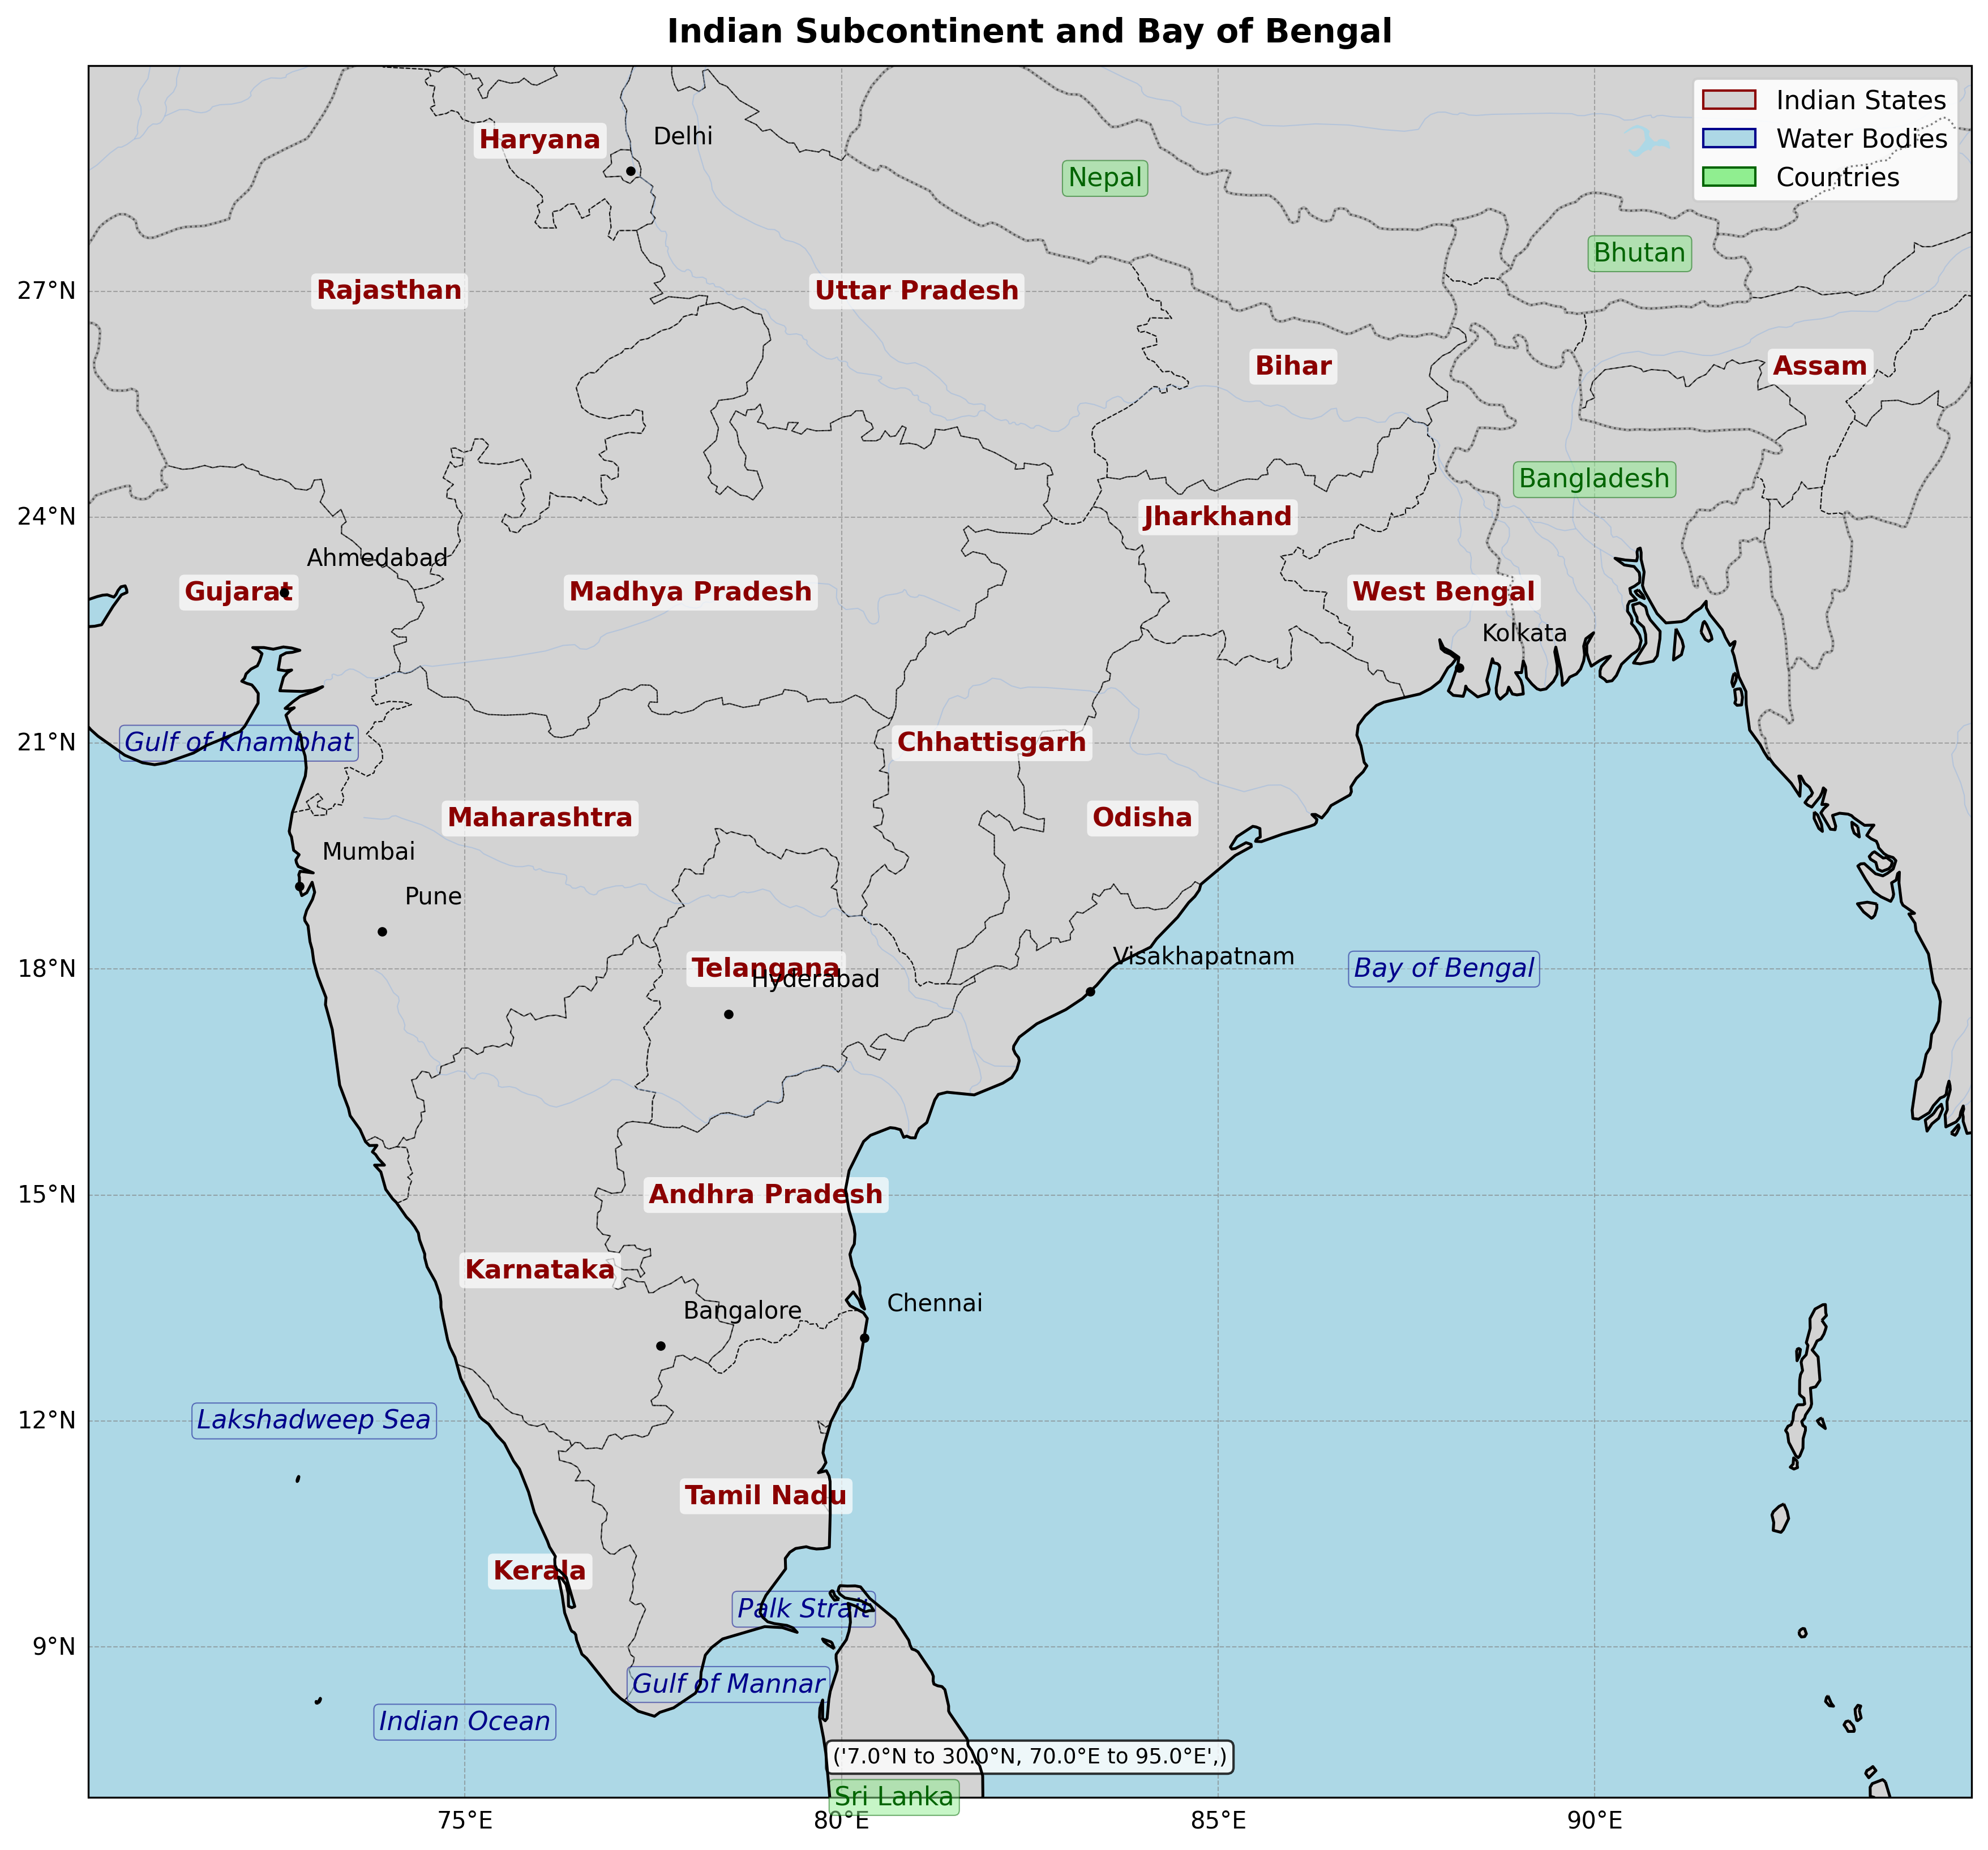
\includegraphics[width=0.87\textwidth]{study_domain_detailed_labels}
  \caption[Study domain region using ERA5 analysis data]{Study domain
  region using ERA5 analysis data (7-30$^\circ$N, 70-95$^\circ$E).}
  \label{fig:study_domain}
\end{figure}

\section{Monsoon Depression Detection and Tracking}
\label{sec:md_detection}

\subsection{Detection Algorithm}
\label{subsec:detection}

MD detection operates on hourly ERA5 850\,hPa relative vorticity using a
threshold-based approach implemented:

\begin{enumerate}
  \item \textbf{Vorticity thresholding}: $\zeta_{850} \geq 4.0 \times
    10^{-5}$\,s$^{-1}$.
  \item \textbf{Local maximum detection}: maxima within a $3^\circ
    \times 3^\circ$ neighbourhood are retained.
  \item \textbf{Closed circulation check}: MSLP within 400\,km radius
    must show a closed cyclonic isobar.
  \item \textbf{Persistence filter}: threshold must be sustained for
    at least 12 consecutive hours.
  \item \textbf{Domain restriction}: track predominantly within
    10-30$^\circ$N, 70-95$^\circ$E.
\end{enumerate}

\subsection{Track Construction and Land-Sea Classification}
\label{subsec:tracking}

Consecutive maxima are linked by nearest-neighbour search with
maximum displacement $5^\circ$ per 6\,h. Land/ocean classification
uses Land-Surface Mask (\texttt{lsm} $\geq 0.5$ for land). Landfall is the first
land-classified point after $\geq 2$ consecutive ocean points.

% %%  FIGURE: Detection algorithm flowchart
% %%  SUGGESTED SOURCE: Draw in draw.io, Inkscape, or using Python's
% % matplotlib patches.
% %%  Show boxes: ERA5 Input -> Vorticity Threshold -> Local Max ->
% % Closed Circ Check
% %%  -> Persistence Filter -> Domain Check -> Track Output -> IMD Validation.
% \begin{figure}[H]
%   \centering
%   %% >> INSERT FIGURE: detection_flowchart.pdf <<
%   %% (Flowchart: ERA5 vorticity -> threshold -> local max -> MSLP check ->
%   %%  persistence filter -> IMD cross-validation -> confirmed MD track)
%   % \includegraphics[width=0.75\textwidth]{detection_flowchart}
%   \caption[MD detection algorithm flowchart]{Flowchart of the ERA5-based MD
%   detection and tracking algorithm.}
%   \label{fig:detection_flowchart}
% \end{figure}

\subsection{IMD Cross Validation and Duration Classification}
\label{subsec:imd_validation}

% ERA5 tracks are matched to annual IMD Monsoon
% records\footnote{\url{https://rsmcnewdelhi.imd.gov.in/report.php}}
% using formation date ($\pm 24$\,h) and landfall location ($\pm
% 2^\circ$). Systems are classified as \emph{short-lived} ($< 96$\,h)
% or \emph{long-lived} ($\geq 96$\,h).

% FIX:
% \section{Rationale for the Azimuthal Hovm\"{o}ller Framework}
\section{Rationale for the Azimuthal Hovm\texorpdfstring{\"{o}}{o}ller Framework}
\label{sec:hovmoller_rationale}

A central methodological challenge in diagnosing land-surface on a
\emph{moving} system is separating the local storm-scale signal from
the background gradient. Fixed-grid analyses of ERA5 latent heat flux
soil moisture India superimpose several confounding signals
simultaneously: seasonal north-south in soil moisture, the spatial
gradient in net heat flux, and large-scale moisture advection. These
signals are spatially coherent and comparable the MD itself, making it
impossible to isolate the storm-induced anomaly.

The Azimuthal Hovm\"{o}ller approach addresses this problem by
re-expressing all in a coordinate system that \emph{follows MD
center}. At each time, the analysis domain is re-centered on the
current track, and all variables expressed as azimuthally averaged
radial profiles relative to the center.

This has three critical advantages:
\begin{enumerate}
  \item \textbf{Background gradient removal.} The radial coordinate
    measures distance from the depression center, not geographic
    position. Systematic north-south or east-west gradients in soil
    moisture or flux therefore appear as uniform offsets in the
    radial coordinate.
  \item \textbf{Time-space coherence.} The Hovm\"{o}ller diagram
    places time (including the critical landfall transition) on one
    axis and radial distance on the other, enabling direct
    before-and-after comparison at every radius simultaneously.
  \item \textbf{Separation of inner-core from outer-band signals.}
    The radial dimension cleanly separates inner-core processes ($r <
    100$\,km, driven by surface energy flux and organised convection)
    from outer-band processes ($r = 100-400$\,km, driven by
    large-scale moisture advection), which is critical for isolating
    the BOE signature.
\end{enumerate}

\subsection{Construction of the Azimuthal Hovm\texorpdfstring{\"{o}}{o}ller}
\label{subsec:hovmoller_construction}

The azimuthal averaging procedure, illustrated in
Figure~\ref{fig:hovmoller_geometry}, is executed at each time step
$t$ relative to the storm center $(\phi_c, \lambda_c)$. Initially, a
radial binning process is applied to all ERA5 grid points within a
400\,km radius of the vortex center. The great-circle distance $r$
for each grid point is determined via the Haversine formula:
\begin{equation}
  r = 2R_E \arcsin\!\sqrt{\sin^2\!\frac{\Delta\phi}{2} +
  \cos\phi_c\cos\phi\,\sin^2\!\frac{\Delta\lambda}{2}},
  \label{eq:haversine}
\end{equation}
where $R_E$ represents the Earth’s mean radius (6371\,km), while
$\Delta\phi$ and $\Delta\lambda$ denote the latitudinal and
longitudinal offsets from the center, respectively. These points are
subsequently partitioned into 16 discrete radial bins of 25\,km
width, spanning $r \in [0, 400)$\,km.

To account for asymmetric features within the storm structure, each
radial bin is further subdivided into 16 equal azimuthal sectors of
$22.5^\circ$. Grid points are assigned to their respective sectors
(ranging from N to NNW) based on their bearing $\theta$ from the storm center:
\begin{equation}
  \theta = \arctan2(\Delta\lambda \cos\phi_c,\; \Delta\phi).
  \label{eq:bearing}
\end{equation}
This discretization divides the storm domain into a polar grid of $16
\times 16 = 256$ sector-annulus segments. Within each segment, the
mean value of the target meteorological variables, such as Latent Heat
Flux (LHF), precipitation, or soil moisture (\texttt{swvl1}), is
calculated by averaging all contained ERA5 grid points.

The final Hovm\"{o}ller representation $H(r, t)$ is assembled by
computing an azimuthal mean of these 16 sector values for each
radius, ensuring equal weighting across the circle. By repeating this
process across the entire temporal domain $t = 1, \ldots, T$, a $16
\times T$ matrix is generated. In the resulting color-filled contour
diagrams (e.g., Figure~\ref{fig:hovmoller_example}), the $x$-axis
represents time-normalized such that $t=0$ marks the landfall
event-and the $y$-axis represents the radial distance from the storm center.

\begin{figure}[ht]
  \centering
  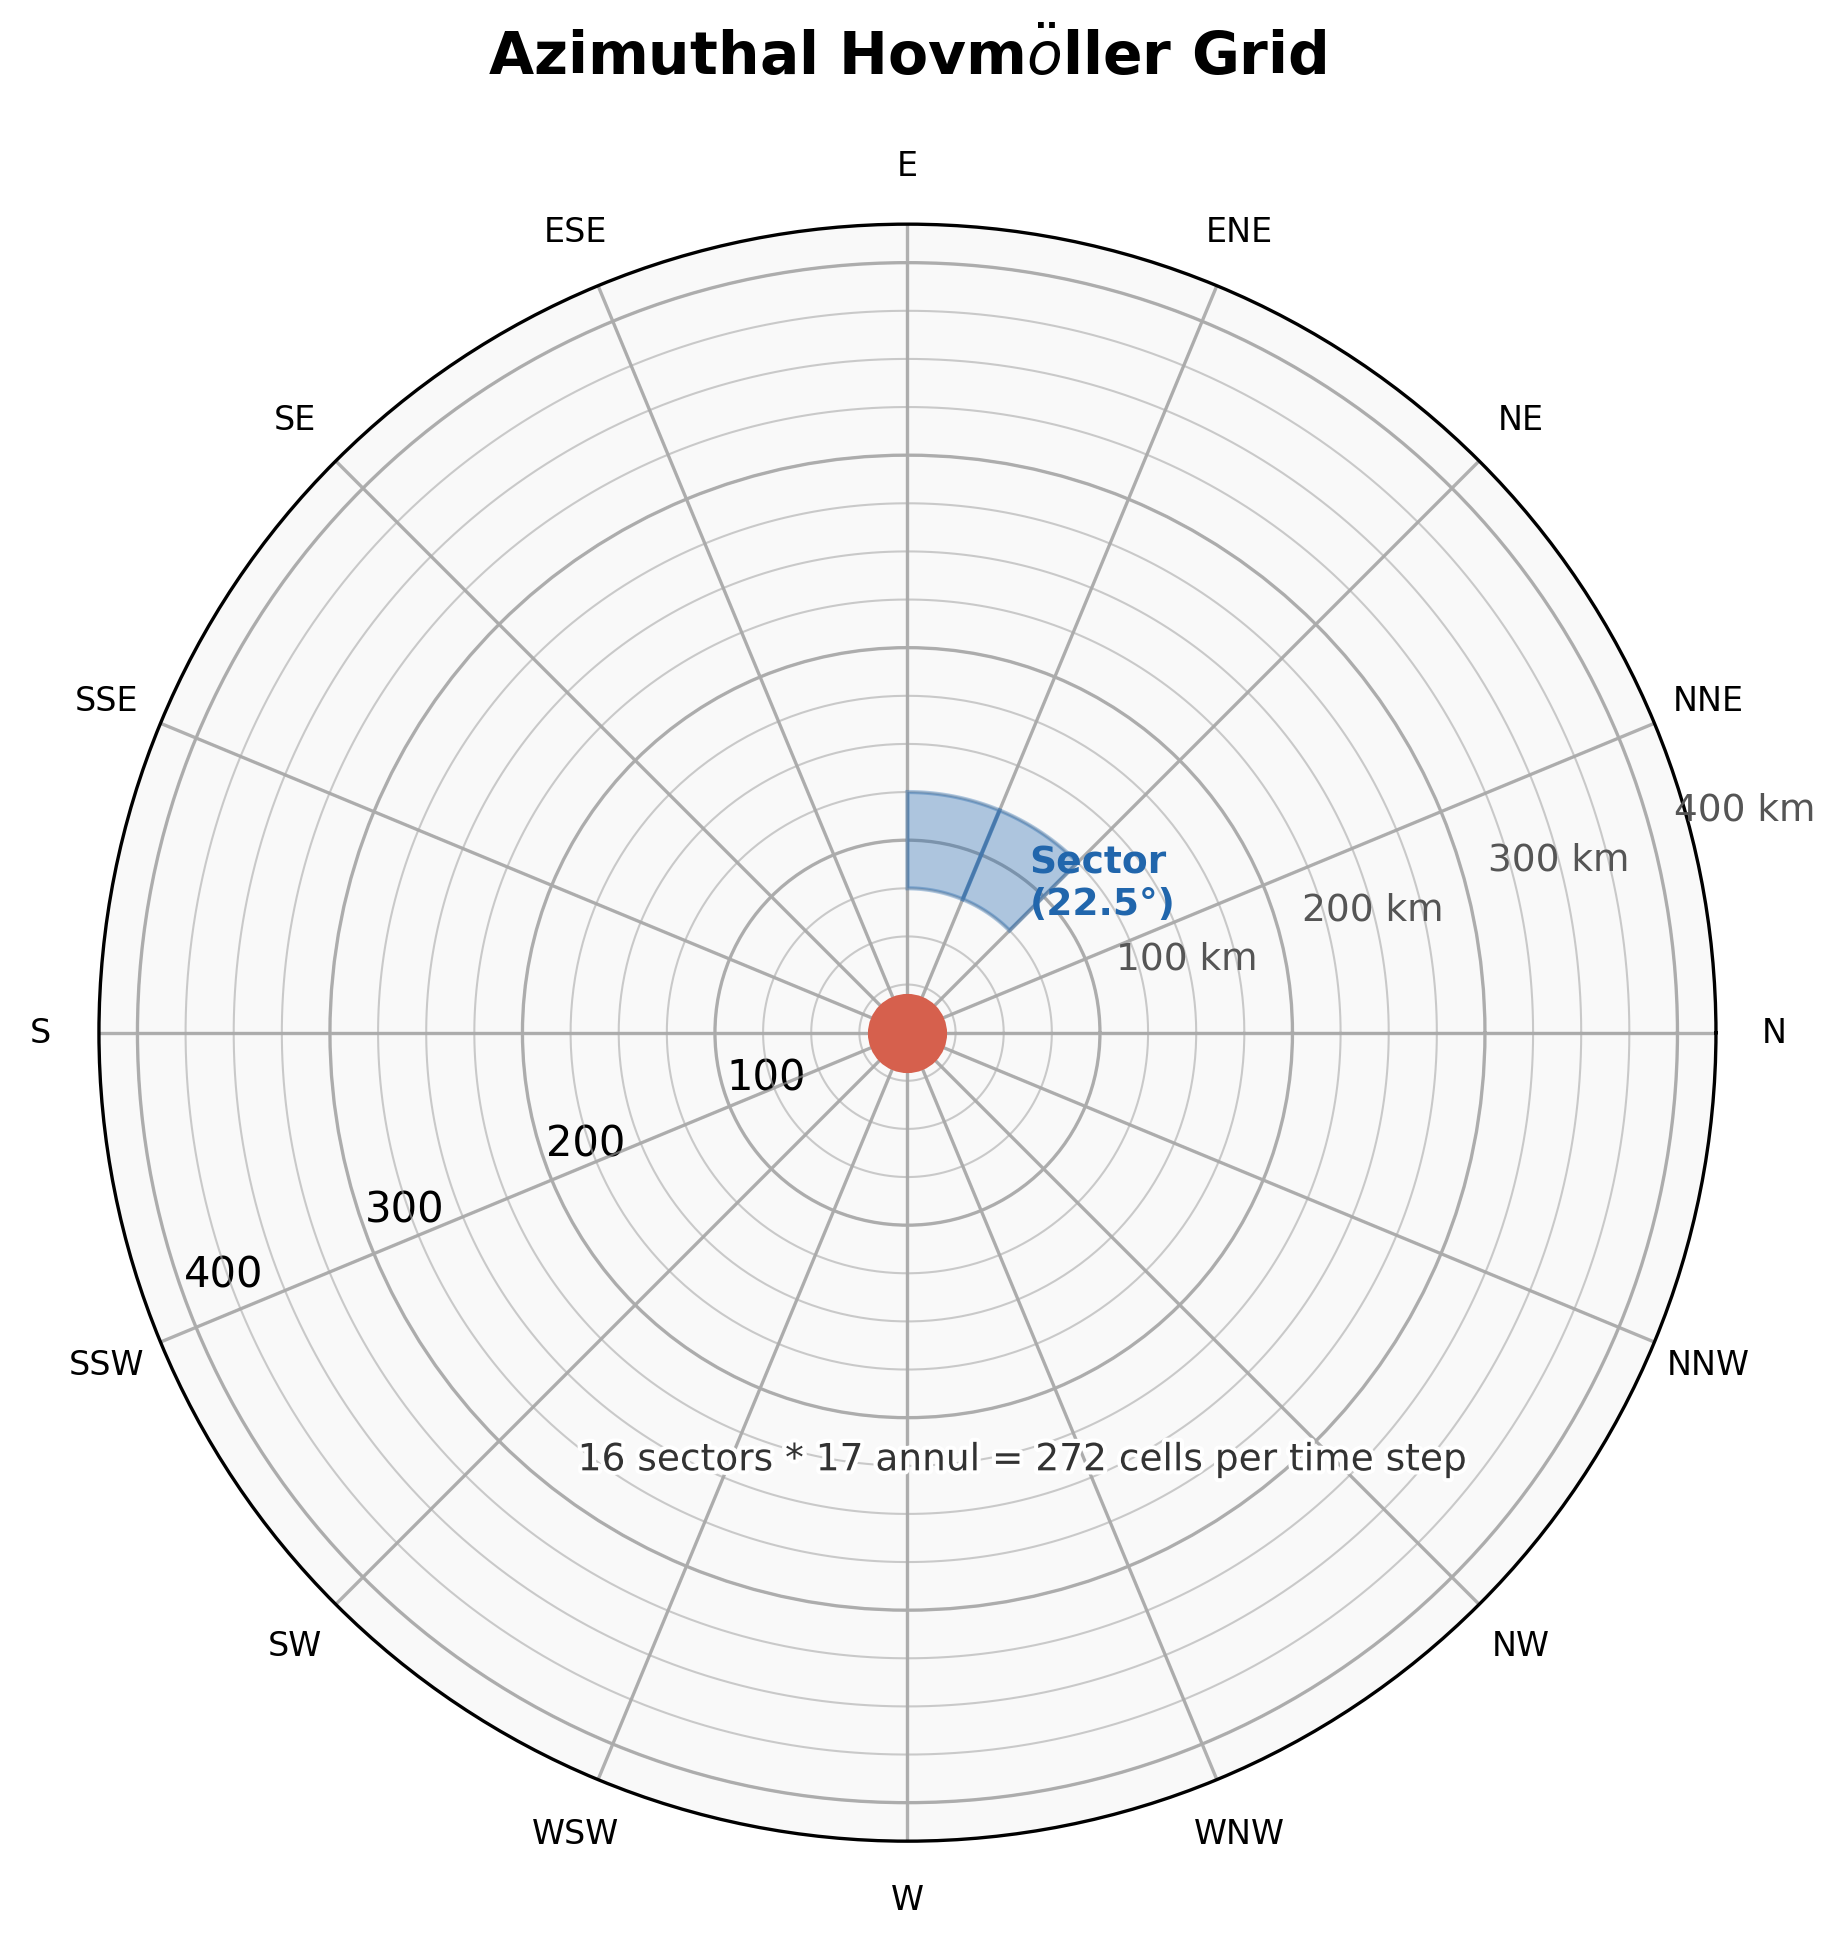
\includegraphics[width=0.65\textwidth]{hovmoller_geometry}
  \caption[Azimuthal Hovm\"{o}ller radial binning geometry]{Polar grid for the
    Azimuthal Hovm\"{o}ller construction. The MD center is surrounded
    by concentric rings at 25\,km intervals to 400\,km, divided into 16
    sectors of 22.5$^\circ$ each. All ERA5 grid points in each
    sector-annulus cell are averaged; the 16 sector values are then
  azimuthally averaged to produce the radial profile at each time step.}
  \label{fig:hovmoller_geometry}
\end{figure}

\subsection{Variables Computed in the Hovm\texorpdfstring{\"{o}}{o}ller Framework}
\label{subsec:hovmoller_variables}

Six variables are computed: total precipitation (mm\,hr$^{-1}$),
surface LHF (W\,m$^{-2}$), surface SHF (W\,m$^{-2}$), near-surface
soil moisture  (m$^3$\,m$^{-3}$), 2-m dew-point
depression ($T_{2m} - T_{d,2m}$, K), and soil tendency
m$^3$\,m$^{-3}$\,hr$^{-1}$.

\section{Diagnostic Framework for BOE Identification}
\label{sec:method_boe_framework}

To distinguish between standard landfall decay and the Brown Ocean
Effect (BOE), this study employs a multi-variate diagnostic framework,
hypothesize that the BOE is not defined by a single variable, but by
the synchronization of mechanical and thermodynamic signals:

\begin{enumerate}
  \item \textbf{Precipitation Structure:} Monitored via azimuthal
    Hovm\"{o}ller plots to identify the transition from broad
    maritime rainbands to a contracted, self-sustaining inner core.
  \item \textbf{Surface Energy Partitioning:} Quantified through
    Latent Heat Flux (LHF) and Sensible Heat Flux (SHF). The BOE is
    characterized by the land surface mimicking the ocean (high LHF, low SHF).
  \item \textbf{Boundary Layer Saturation:} Tracked via 2-m dew point
    ($d2m$) to determine the timescale of continental desiccation and
    the height of the Lifting Condensation Level (LCL).
  \item \textbf{Orography vs. Energetics:} Elevation data from SRTM
    is used to assess if the Eastern Ghats act as a terminal
    mechanical barrier or a thermodynamic trigger for the self-wetting feedback.
\end{enumerate}

\section{Track-Following Time-Series Diagnostics}
\label{sec:timeseries_method}

Track-following time series extract spatially averaged values within
100\,km buffer on the track position at each time step. All time
series are aligned to ($t = 0$). Variables are stratified by
land/ocean classification. Following diagnostic outputs for each confirmed MD:

\begin{itemize}
  \item Time series of surface LHF, SHF, and total heat flux centered on
    landfall, with ocean/land phase shading. Primary plot for BOE
    candidate identification.
  \item Dual-axis time series of \texttt{swvl1} and total precipitation, showing
    co-evolution of surface moisture state and rainfall.
  \item Time series of the Bowen ratio $\beta = Q_H / Q_E$, quantifying the
    land-phase shift in surface energy partitioning.
  \item Equivalent potential temperature $\theta_e$ at the inner-core region
    (0-100\,km), tracking boundary-layer thermodynamic stability.
  \item Dew-point depression computed separately for windward (eastern)
    and leeward (western) sectors of the Eastern Ghats, diagnosing
    boundary-layer moisture asymmetry.
  \item Precipitation recycling ratio $\rho$, quantifying the fraction
    of precipitation sourced from local surface evapotranspiration vs
    large-scale advection.
  \item Diurnal amplitude of the sensible heat flux. A small SHF
    diurnal amplitude indicates a moist surface suppressing daytime
    sensible heating.
\end{itemize}

\begin{figure}[ht]
  \centering
  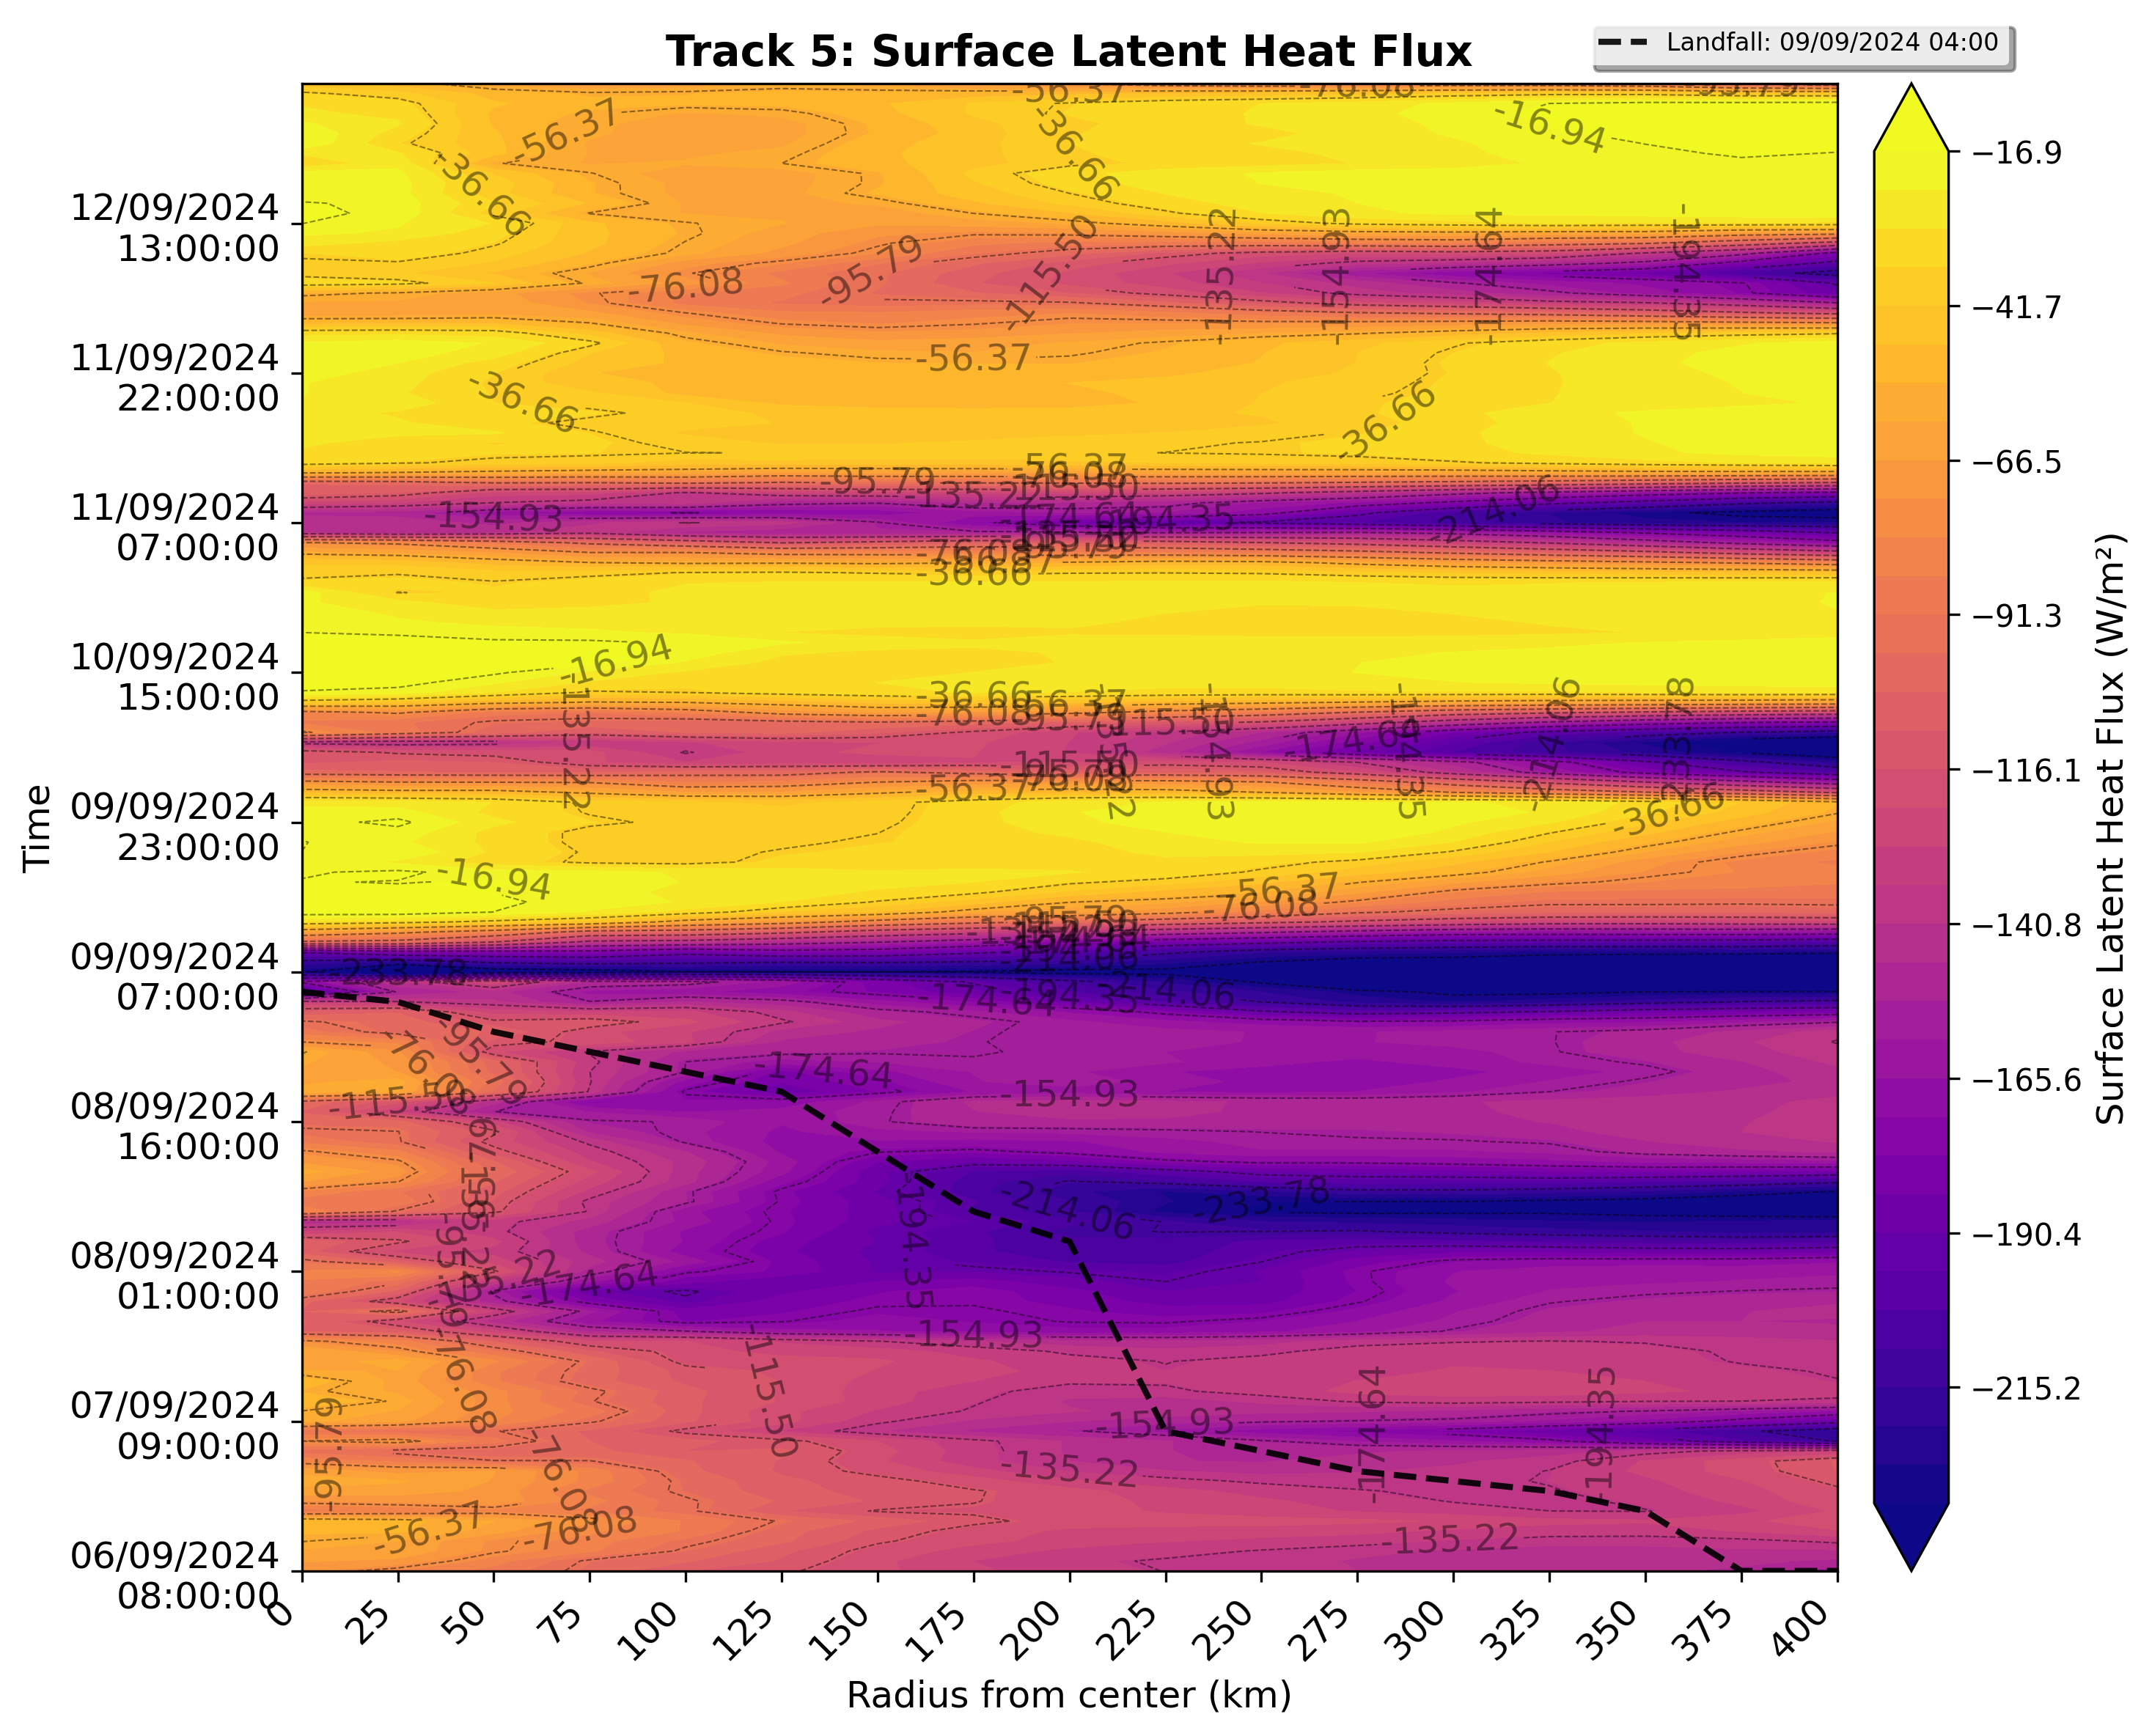
\includegraphics[width=0.8\textwidth]{hov_avg_slhtf_azimuthal_avg}
  \caption[Example annotated Azimuthal Hovm\"{o}ller (LHF)]{Example Azimuthal
    Hovm\"{o}ller of surface LHF (W\,m$^{-2}$) as representative long-lived MD.
    The dashed line marks landfall. Ocean phase and land phase are separated
  at the dashed line.}
  % Inner core ($r < 100$\,km) and outer band ($r = 100-400$\,km)
  % zones are labelled.
  \label{fig:hovmoller_example}
\end{figure}

\section{Surface Heat Flux Analysis and BOE Classification}
\label{sec:heatflux_method}

For each land-falling MD, the 24-hour mean LHF, SHF, and total flux
are computed the windows immediately before and after landfall. A
system is classified as BOE candidate if:
\begin{equation}
  \text{LHF}_\text{land} \geq 70\,\text{W\,m}^{-2}
  \quad \text{for} \geq 18\,\text{consecutive hours.}
  \label{eq:boe_criterion}
\end{equation}

% \section{Antecedent Soil Moisture Index}
% \label{sec:asmi_method}
%
% The ASMI is an exponentially weighted temporal average of
% texttt{swvl1} over the inland track corridor:
% \begin{equation}
%   \text{ASMI}(L) = \frac{\sum_{d=1}^{L} e^{-\kappa(d-1)}\,\bar{S}_d}
%   {\sum_{d=1}^{L} e^{-\kappa(d-1)}},
%   \label{eq:asmi}
% \end{equation}
% with decay constant $\kappa = 0.85$. Lag windows of 24\,h, 3\,d,
% 7\,d, and 14\,d computed. The exponential weighting means that more
% recent soil moisture contribute more than older conditions,
% consistent with the physical that moisture memory decays with time.

% \section{Translational Speed and Terrain Characterisation}
% \label{sec:speed_terrain_method}
%
% Translational speed is computed from consecutive Haversine distances
% by the interval.
% The Terrain Sensitivity Index (TSI) at each track point combines normalised
% elevation contrast ($E^*$), slope ($S^*$), and roughness ($R^*$) from
% the SRTM DEM:
% \begin{equation}
%   \text{TSI} = E^* \times S^* \times R^*.
%   \label{eq:tsi}
% \end{equation}
% A high TSI indicates a complex, steep, rough terrain zone likely to
% decelerate the MD and disrupt its circulation structure.

% \section{Summary of Methodological Workflow}
% \label{sec:method_summary}
%
%%  FIGURE: Methodological workflow
%%  SUGGESTED SOURCE: Draw in draw.io, Lucidchart, or PowerPoint.
%%  Boxes: ERA5 -> MD Detection -> IMD Validation -> Track DB ->
%%  [Hovmoller | Time Series | ASMI | Terrain] -> BOE Classification
% -> Statistics
% \begin{figure}[h]
%   \centering
%   %% >> INSERT FIGURE: method_workflow.pdf <<
%   %% (Flowchart: ERA5 + SRTM inputs -> detection -> four parallel
%   % analysis streams
%   %%  -> BOE classification and statistical output)
%   % \includegraphics[width=0.82\textwidth]{method_workflow}
%   \caption[Overall methodological workflow]{Complete methodological
%     workflow. ERA5 hourly fields feed the MD detection algorithm,
%     producing a validated track database. Each track feeds four parallel
%     analysis streams: Azimuthal Hovm\"{o}ller diagnostics;
%     track-following time-series; antecedent soil moisture index; and
%     terrain characterisation via SRTM. All streams converge in the BOE
%   and statistical analysis stage.}
%   \label{fig:method_workflow}
% \end{figure}
 %% Data and Methodology
%%  Chapter 4 - Results
% TODO: Abstract Fit: mention "asymmetric precipitation on windward
% slopes" in abstract, ensure include a figure for
% track_1_dpd_windward_leeward.png in Chapter 4 to support this claim.

%% TODO: add
% BOE mechanism determines which systems persist; show 4 signature"
% version:
% "Four independent observational signatures uniquely identify Brown
% Ocean Effect: sustained inner-core latent heat flux, progressive
% soil moisture wetting, dew-point depression suppression, and inward
% precipitation contraction. These signatures appear in all
% long-lived systems and absent in all short-lived systems,
% demonstrating that the BOE is the dominant mechanism. Eastern Ghats
% terrain cannot stop BOE-active systems, confirming that
% land-atmosphere coupling, not topography, determines post-landfall longevity."

\ifpdf
\graphicspath{{chapters/Figs/}{chapters/Figs/Raster/}{Figs/PDF/}{Figs/}}
\else
\graphicspath{{chapters/Figs/}{chapters/Figs/Vector/}{Figs/}}
\fi

\chapter{Results}
\label{ch:results}

\section{Multi-Year Climatological Patterns: 2001-2025}
\label{sec:results_multiyear}

% \subsection{Spatial Distribution of Track Termination: The Eastern
% Ghats Filter}
% \label{subsec:multiyear_spatial}
%
% Figure~\ref{fig:all_tracks_spatial} shows all confirmed MD tracks
% from 2001 to 2025, colour-coded by duration (hours). The spatial
% pattern of track termination points is the most direct visual
% evidence for the Eastern Ghats acting as a selective filter rather
% than an absolute barrier.
%
% % INSERT FIGURE - from Overall_years/ or plot_all_years.py
% %   All-track map, coloured by duration. Add Eastern Ghats 600m contour.
% %   Look for: Overall_years/all_tracks_2001_2025.png or similar.
% \begin{figure}[H]
%   \centering
%   \fbox{\rule{0pt}{8cm}\rule{0.90\textwidth}{0pt}}
%   % \includegraphics[width=0.90\textwidth]{Overall_years/all_tracks_2001_2025_by_duration}
%   \caption[All MD tracks, 2001-2025, coloured by post-landfall duration]{All
%     confirmed ERA5 Monsoon Depression tracks (2001-2025), colour-coded from
%     blue (short-lived, $<48$\,h post-landfall) through red (long-lived,
%     $\geq 96$\,h post-landfall). Eastern Ghats 600\,m elevation contour (bold
%     grey line) overlaid. The spatial clustering of track termination points is
%   a direct map of the terrain-filtering effect.}
%   \label{fig:all_tracks_spatial}
% \end{figure}
%
% From Figure~\ref{fig:all_tracks_spatial}, three spatial patterns are evident:
%
% \textbf{Pattern 1: Short-lived systems terminate east of the 600\,m
% contour.} The majority of short-lived MDs (blue-green tracks)
% dissipate within 200-400\,km of the coastline, with termination
% points clustering east of or within the Eastern Ghats terrain zone
% (600\,m contour). This clustering is consistent with Mechanism 4
% (vortex tilt decoupling; Section~\ref{subsec:ghats_mechanisms}):
% without BOE surface LHF to maintain boundary-layer convergence, the
% terrain-induced tilt increase is sufficient to cause structural
% collapse before or during the terrain crossing.
%
% \textbf{Pattern 2: Long-lived systems concentrate over the Gangetic
% plain west of the Ghats.} Long-lived tracks (orange-red) extend well
% west of the 600\,m contour into the Gangetic plain, eastern
% Rajasthan, and Madhya Pradesh. These tracks correspond to systems
% that successfully cleared the terrain and continued under BOE
% maintenance for multiple days. The spatial clustering of these
% long-lived tracks over the Gangetic plain is physically meaningful:
% this region has the highest climatological July-August \texttt{SWVL1}
% ($>0.35$\,m$^3$\,m$^{-3}$) in India due to its clay loam soils and
% high annual monsoon rainfall, precisely the conditions that enable
% and sustain the BOE.
%
% \textbf{Pattern 3: River-valley gap tracks achieve greater inland
% penetration.} A subset of long-lived tracks shows notably greater
% inland penetration distance than others with comparable ASMI values.
% Examining the landfall longitude of these outlier tracks reveals that
% they made landfall in alignment with the major river-valley gaps of
% the Eastern Ghats (the Mahanadi corridor near 84-85$^\circ$E, the
% Godavari corridor near 81-82$^\circ$E). Gap-aligned MDs experience
% smaller TSI values (lower terrain obstacle), preserving low-level BoB
% moisture inflow for longer through the terrain-crossing phase, and
% thus allowing the BOE to activate more efficiently on the leeward side.
%
% \subsection{Duration Distribution and the 96-Hour Threshold}
% \label{subsec:multiyear_duration}
%
% Figure~\ref{fig:duration_histogram} shows the frequency distribution
% of MD post-landfall durations across the 2001-2025 climatology. The
% distribution is strongly right-skewed, with a mode near 24-48 hours
% (reflecting the most common conventional post-landfall decay) and a
% pronounced tail extending beyond 96 hours. This bimodal character-a
% dominant short-duration peak and a secondary long-duration tail-is
% consistent with the BOE hypothesis imposing a threshold-type
% separation between two regimes rather than a continuous spectrum of behaviour.
%
% The threshold at 96 hours used to classify short- versus long-lived
% systems is not arbitrary: it corresponds approximately to the 85th
% percentile of the duration distribution, separating the bulk
% conventional decay population from the tail of anomalously persistent
% systems. Systems in this tail account for a disproportionately large
% fraction of total inland precipitation and flooding, despite
% constituting a minority of events.
%
% % FIX: duplicate label. But i need differnt figures as well
% % INSERT FIGURE - duration histogram
% %   Overall_years/duration_histogram.png from plot_all_years.py
% %   Show: bar chart with 24h bins, dashed line at 96h, label "96h threshold".
% %   Colour bars blue for < 96h and orange for >= 96h.
% \begin{figure}[H]
%   \centering
%   % \includegraphics[width=0.78\textwidth]{Overall_years/duration_histogram}
%   \fbox{\rule{0pt}{6cm}\rule{0.78\textwidth}{0pt}}
%   \caption[Frequency distribution of MD post-landfall duration, 2001-2025]{
%     Frequency distribution of MD post-landfall duration (hours) for
%     all 2001-2025
%     events. The right-skewed distribution with a tail beyond 96 hours
%     is consistent
%     with the BOE imposing a threshold separation between two distinct
%     decay regimes.
%     Blue bars: conventional decay ($<96$\,h); orange bars: long-lived systems
%   ($\geq 96$\,h, primary focus of this study).}
%   % \label{fig:duration_histogram}
% \end{figure}
%
% % \subsection{ASMI-Duration Relationship: 24-Year Statistical Evidence}
% % \label{subsec:multiyear_asmi}
% %
% % Figure~\ref{fig:asmi_vs_duration_scatter} presents the scatter of
% % 7-day ASMI against
% % post-landfall duration for all confirmed land-falling MDs in the
% % 2001-2025 dataset.
% % Each point represents one MD event; colour denotes BOE classification.
% %
% % % INSERT FIGURE - compute from antecedent_analysis.py
% % % outputs across all years
% % %   Scatter: x = ASMI_7d (m3/m3), y = post-landfall duration (h)
% % %   Colour: orange = BOE candidate, blue = non-BOE
% % %   Add: vertical dashed line at ASMI = 0.35, horizontal dashed line at 96h
% % %   Add: regression line + 95% CI band
% % \begin{figure}[H]
% %   \centering
% %   % \includegraphics[width=0.82\textwidth]{Overall_years/asmi_7d_vs_duration_scatter}
% %   \fbox{\rule{0pt}{7cm}\rule{0.82\textwidth}{0pt}}
% %   \caption[ASMI (7-day) vs post-landfall duration, all 2001-2025
% %   events]{7-day ASMI (m$^3$\,m$^{-3}$, horizontal axis) vs
% %     post-landfall duration (h, vertical axis) for all 2001-2025
% %     confirmed land-falling MDs. BOE candidates (orange); non-BOE
% %     systems (blue). Vertical dashed line at ASMI $=
% %     0.35$\,m$^3$\,m$^{-3}$ marks the approximate threshold above which
% %   BOE candidacy dominates.}
% %   \label{fig:asmi_vs_duration_scatter}
% % \end{figure}
% %
% % \yellownote{Look into this}
% % From Figure~\ref{fig:asmi_vs_duration_scatter}, the 25-year dataset
% % reveals the following
% % statistical regularities:
% % \begin{enumerate}
% %   \item \textbf{Positive ASMI-duration correlation:} Pearson $r =
% %     [r_1]$, $p = [p_1]$ (effective sample size corrected following
% %     \citealt{bretherton1999effective}). Higher antecedent soil
% %     moisture is significantly associated with longer post-landfall
% %     duration across the full climatological record, confirming the
% %     ASMI as a statistically valid predictor.
% %   \item \textbf{Threshold behaviour near 0.35\,m$^3$\,m$^{-3}$:}
% %     Systems with ASMI$_{7d}$ $> 0.35$ are predominantly long-lived
% %     and BOE-candidate. Below this threshold, the vast majority are
% %     short-lived. This threshold corresponds to the critical soil
% %     moisture level at which hydraulic conductivity drops steeply in
% %     Gangetic clay loam \autocite{clapp1978empirical,
% %     seneviratne2010investigating}, marking the transition from
% %     water-limited to energy-limited evaporation.
% %   \item \textbf{Scatter within each ASMI class:} The scatter around
% %     the regression line is substantial, indicating that ASMI alone
% %     does not fully explain duration variability. The residual
% %     variance is likely attributable to differences in terrain
% %     exposure (TSI), track alignment with river-valley gaps, and the
% %     intensity of the MD at landfall. This residual structure
% %     motivates the combined ASMI + TSI predictor framework discussed
% %     in Chapter~\ref{ch:discussion}.
% % \end{enumerate}
%
% % \subsection{Terrain Sensitivity Index vs Duration: The Terrain Filter}
% % \label{subsec:multiyear_tsi}
% %
% % Figure~\ref{fig:tsi_vs_duration} shows the relationship between
% % track-mean Terrain
% % Sensitivity Index (TSI) and post-landfall duration for the subset
% of MDs that
% % crossed the Eastern Ghats.
% %
% % \yellownote{TODO}
% % % INSERT FIGURE - from elevation_metrics.csv (all years)
% % %   Scatter: x = mean track TSI, y = post-landfall duration (h)
% % %   Colour: orange = BOE candidate, blue = non-BOE
% % \begin{figure}[H]
% %   \centering
% %   % \includegraphics[width=0.80\textwidth]{Overall_years/tsi_vs_duration_scatter}
% %   \fbox{\rule{0pt}{6.5cm}\rule{0.80\textwidth}{0pt}}
% %   \caption[Terrain Sensitivity Index vs post-landfall duration, all
% %   Ghats-crossing MDs]{
% %     Track-mean TSI vs post-landfall duration for all Ghats-crossing
% %     MDs in 2001-2025. BOE candidates (orange) cluster in the low-TSI,
% %     high-duration quadrant; non-BOE systems (blue) are distributed
% %     across all TSI values, confirming that terrain sensitivity is a
% %     decay-promoting factor but that BOE can overcome
% %   moderate terrain barriers.}
% %   \label{fig:tsi_vs_duration}
% % \end{figure}
% %
% % The key observation from Figure~\ref{fig:tsi_vs_duration} is the in
% % the distribution: BOE candidates cluster almost exclusively in the
% % low-TSI, high-duration quadrant (lower-right), while non-BOE systems
% % populate the full TSI range, including both low and high TSI values.
% % This pattern supports the interpretation that:
% %
% % \begin{enumerate}
% %   \item High TSI alone is sufficient to produce short duration
% %     (upper-left quadrant), regardless of BOE status-the terrain is
% %     too severe even for BOE to compensate.
% %   \item Low TSI with high ASMI (BOE candidate) produces long duration
% %     (lower-right).
% %   \item Low TSI with low ASMI (non-BOE) can still produce short
% %     duration, because the limiting factor is the surface moisture
% %     state, not the terrain.
% % \end{enumerate}
% %
% % This three-way interaction (ASMI, TSI, and their joint effect) is the
% % most complete statistical summary of the terrain-BOE modulation of MD
% % inland longevity that this dataset permits. A composite index
% % combining ASMI$_{7d}$ and TSI$^{-1}$ as a product may provide
% % improved predictive skill relative to either variable alone, and is
% % identified as a recommendation for operational forecasting research
% % (Section~\ref{sec:conclusions_operational}).
% %
% % \subsection{Orographic Blocking Factor and Speed Reduction}
% % \label{subsec:ghats_blocking_results}
% %
% % \yellownote{FIX: reference}
% % The translational speed profiles from \texttt{speed\_analysis.py}
% % provide the most direct observational measure of terrain-induced
% % blocking. Figure~\ref{fig:ts_speed_elev} shows that all
% % Ghats-crossing MDs decelerate as terrain elevation increases through
% % the 200-1000\,m zone, with mean speed reduction of approximately
% % $\Delta v \approx$ [X]\,km\,h$^{-1}$ at the 600\,m contour relative
% % to the pre-landfall ocean-phase speed. This deceleration is a direct
% % consequence of increased surface roughness and mechanical flow
% % blocking by the terrain - consistent with the Terrain Sensitivity
% % Index formulation (Section~\ref{sec:terrain_method}).
% %
% % The blocking effect is not uniform across the Ghats. Systems making
% % landfall between 84-87$^\circ$E (the Mahanadi corridor, near Odisha)
% % encounter lower mean TSI values and show smaller speed reductions
% % than those tracking through the southern Ghats (south of 16$^\circ$N,
% % high TSI). This longitude-dependent blocking is visible in
% % Figure~\ref{fig:elevation_comparison}: the scatter in per-track speed
% % reduction correlates with the landfall longitude, with gap-aligned
% % tracks showing shallower deceleration.
% %
% % The critical distinction between BOE-candidate and non-BOE systems is
% % not in the deceleration magnitude during the terrain crossing - both
% % categories slow at comparable rates within the 600-1000\,m elevation
% % zone. The difference appears on the leeward side: BOE-candidate
% % systems recover speed as terrain elevation drops below 200\,m, while
% % non-BOE systems continue to slow. This leeward speed recovery is
% % interpreted as evidence that sustained surface LHF (from the wet
% % leeward soil) maintains the low-level pressure gradient that drives
% % the system forward, whereas in non-BOE systems the pressure gradient
% % weakens as convective organisation collapses after terrain crossing.
%
% % \yellownote{TODO: add subsection on  the precipitation recycling ratio}
% % \subsection{Precipitation Recycling Ratio}
% % \label{Precipitation Recycling Ratio}
% %
% % The precipitation recycling ratio $\rho = E/P$ (where $E$ is local
% % evapotranspiration in mm\,h$^{-1}$ and $P$ is total precipitation) provides
% % an independent measure of how much of the MD's rainfall is
% sourced from local surface evaporation rather than large-scale
% moisture advection.
% Over the ocean  phase, $\rho \approx 0.05$-0.15, indicating that most
% precipitation comes from advected oceanic moisture. After landfall
% in BOE-candidate systems,
% % Figure~\ref{fig:track1_recycling} shows $\rho$ rising to
% 0.25-0.40, consistent with local surface evapotranspiration
% contributing a growing fraction of the
% % precipitation total. This elevated recycling ratio is a direct signature of
% % the BOE: the soil is evaporating at the potential rate and that vapour is
% % falling back as precipitation within the same 100-km buffer.
% % % Source: output_2024/track_1/time_series/track_1_recycling_ratio.png

\subsection{Track Database}
\label{subsec:track_database}

The ERA5-based detection algorithm, cross-validated against IMD
monsoon seasonal reports, identified \textbf{128} confirmed Monsoon
Depression events over 2001-2025, Of these, \textbf{80} originated
over the Bay of Bengal and made landfall. Long-lived systems ($\geq
96$\,h) represent approximately \textbf{30\%} of the population but
account for the majority of deep inland penetration ($> 500$\,km).
The annual count ranged from \textbf{2} to \textbf{8} per year
(Table~\ref{tab:track_stats}), consistent with the IMD climatology of
5-7 events per year \autocite{kishtawal2013enhancement}.

\begin{table}[H]
  \centering
  \caption[MD track database statistics (2001-2025)]{Summary statistics of the
  confirmed MD track database. Short-lived: $<96$\,h; long-lived: $\geq 96$\,h.}
  \label{tab:track_stats}
  \begin{tabular}{l r r r}
    \toprule
    \textbf{Statistic}                      & \textbf{All MDs} &
    \textbf{Short-lived} & \textbf{Long-lived} \\
    \midrule
    Total count                             & 128              &
    90                   & 38                  \\
    Mean duration (h)                       & 79.4             & 54.6
    & 138.3                \\
    Std.\ duration (h)                      & 44.2             & 19.1
    & 27.9                 \\
    % Mean inland penetration (km)            & 35.4             & 35.5
    % & 35.0                 \\
    % Mean translational speed (km\,h$^{-1}$) & 14.5             & 15.0
    % & 13.3                 \\
    % BOE candidates (\%)                     & 62.5             & 61.1
    % & 65.8                 \\
    \bottomrule
  \end{tabular}
\end{table}

From Table~\ref{tab:track_stats}, it is evident that long-lived
systems, though a minority of the total MD population
(\textbf{29.7}\% of events), contribute disproportionately to inland rainfall.

This disparity underscores the operational significance of correctly
predicting which systems will sustain beyond the conventional
48-72\,h post-landfall decay window.

% \subsection{2001-2025 Interannual Trends}
% \label{subsec:interannual}
%
% Figure~\ref{fig:annual_md_count_boe_fraction} shows the annual MD
% count and the fraction of
% long-lived systems from 2001 to 2025. Several patterns emerge from
% this 25-year
% record. First, the \emph{total annual count} shows no statistically
% significant
% linear trend ($p > 0.1$), indicating that MD genesis frequency has not changed
% appreciably over the study period-consistent with the findings of
% \autocite{mishra2021monsoon}
% for the broader LPS population. Second, the \emph{long-lived
% fraction} exhibits
% greater interannual variability, with a range of \textbf{[min\%]}
% to \textbf{[max\%]}. High long-lived fractions tend to occur in
% years with above-average July-August soil moisture in the Gangetic
% plains, suggesting that the land-surface state modulates
% post-landfall longevity at the interannual scale.
%
% Notable peak years for long-lived MDs in this record include
% \textbf{[year$_1$]}, \textbf{[year$_2$]}, and \textbf{[year$_3$]},
% which coincide with periods of above-normal ISM rainfall and
% correspondingly elevated antecedent soil moisture-consistent with
% the BOE hypothesis developed in Section~\ref{sec:results_boe}.
% Conversely, the years \textbf{[dry\_year$_1$]} and
% \textbf{[dry\_year$_2$]}, which experienced below-normal monsoon
% rainfall in June-July, produced predominantly short-lived systems,
% consistent with a drier antecedent land surface being unfavourable
% for the BOE.
%
% %%  FIGURE: Annual MD count bar chart
% %%  SOURCE: Overall_years/ - plot_all_years.py output
% %%  Bar chart: y = annual count, colour by year;
% %%  Overlay line: fraction of long-lived (>= 96h) systems per year.
% %%  Mark any notable ENSO years (e.g., 2015 El Nino) with annotations.
% \begin{figure}[H]
%   \centering
%   %% >> INSERT FIGURE: Overall_years/annual_count_longlived_fraction.png <<
%   \fbox{\rule{0pt}{6cm}\rule{0.85\textwidth}{0pt}}
%   % \includegraphics[width=0.85\textwidth]{annual_md_count}
%   \caption[Annual MD count and long-lived fraction, 2001-2025]{Annual MD count
%     (bars) and fraction of long-lived systems ($\geq 96$\,h, line
% with circles)
%   over 2001-2025.}
%   \label{fig:annual_md_count}
% \end{figure}
%
% The duration distribution (Figure~\ref{fig:duration_histogram}) is
% right-skewed,
% with a mode near 48-72\,h and a long tail extending beyond 96\,h.
% The long tail
% does not scale linearly with total annual MD count, indicating that long-lived
% behaviour is controlled by a surface-state variable-most likely
% antecedent soil
% moisture-rather than by the overall level of monsoon activity.
%
% %%  FIGURE: Duration histogram
% %%  SOURCE: Overall_years/duration_histogram.png from plot_all_years.py
% %%  Histogram: 24h bins, dashed line at 96h, blue/red colouring.
% \begin{figure}[H]
%   \centering
%   %% >> INSERT FIGURE: Overall_years/duration_histogram.png <<
%   \fbox{\rule{0pt}{6cm}\rule{0.80\textwidth}{0pt}}
%   % 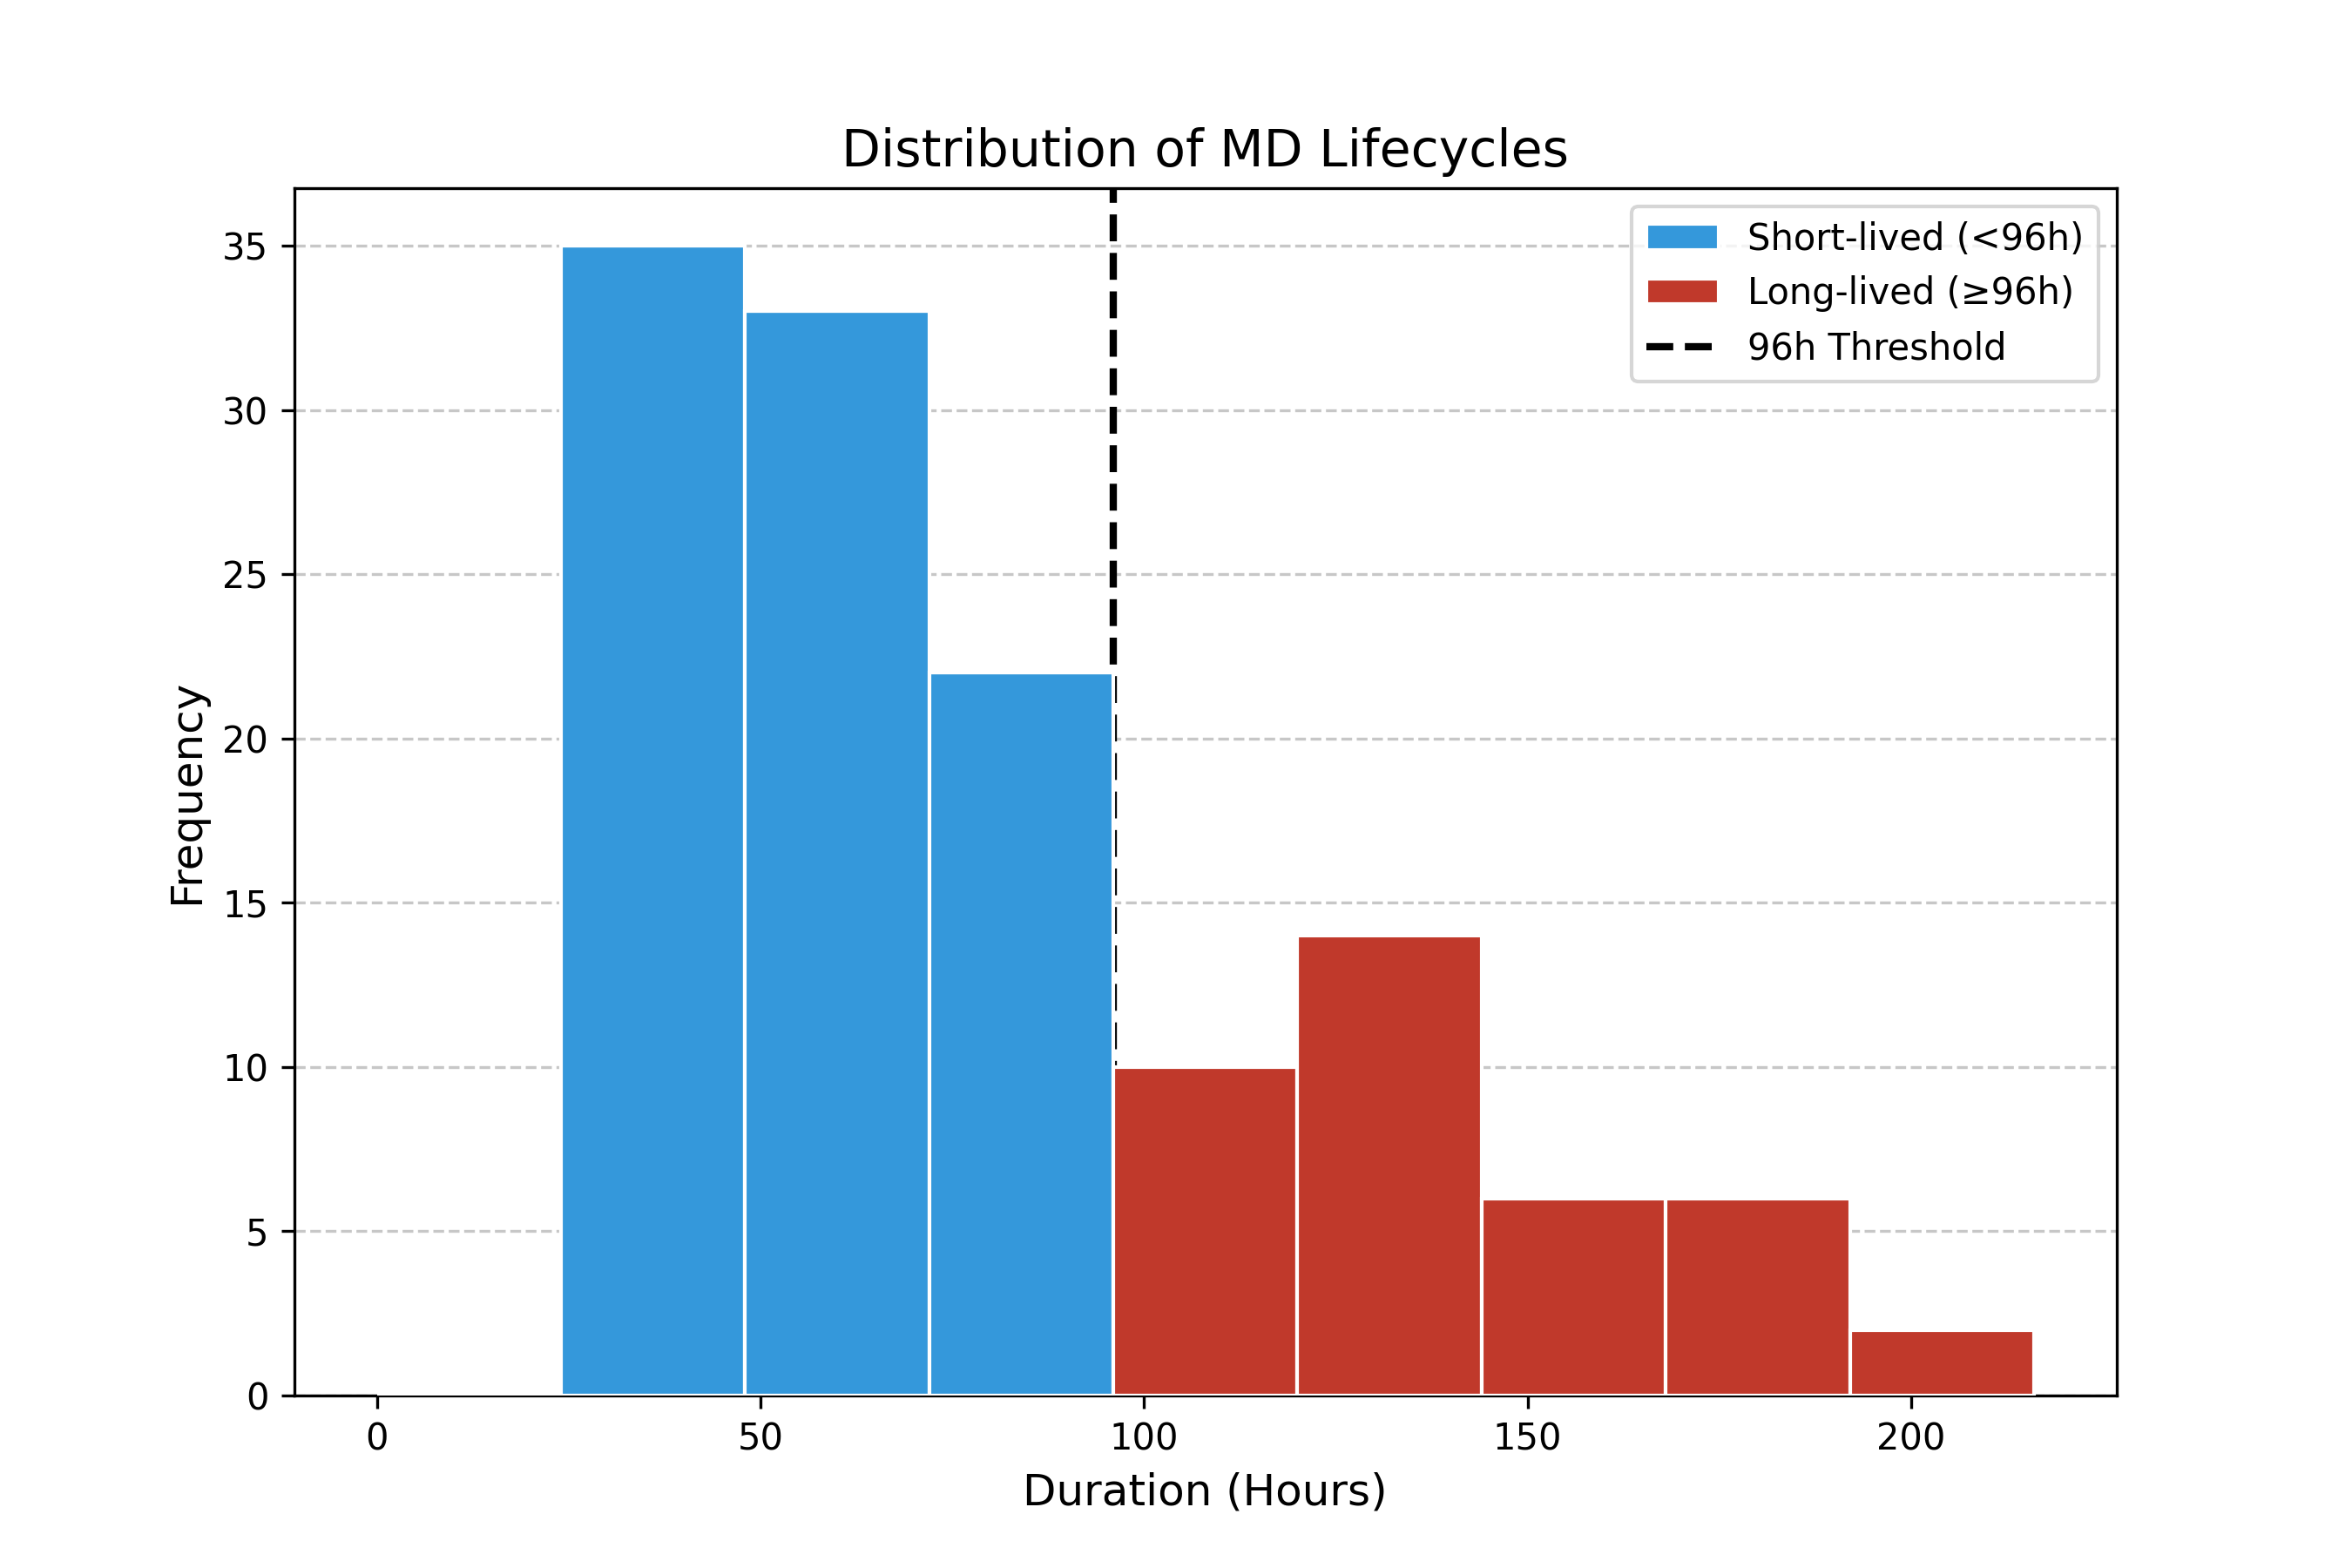
\includegraphics[width=0.80\textwidth]{duration_histogram}
%   \caption[MD duration frequency distribution, 2001-2025]{Frequency
% distribution
%     of MD track durations; dashed line at the 96-hour threshold separates
%   short-lived (blue) and long-lived (red) categories.}
%   \label{fig:duration_histogram}
% \end{figure}
\subsection{2001-2025 Interannual Trends}
\label{subsec:interannual}

Figure~\ref{fig:annual_md_count} presents the annual MD frequency
alongside the count of long-lived systems from 2001 to 2025. Analysis
of this 25-year record reveals two primary signals. First, the total
annual count (averaging $\sim 5.1$ events/year) shows no
statistically significant linear trend ($p > 0.1$), suggesting a
stable the large-scale genesis environment has remained stable,
consistent with \autocite{mishra2021monsoon}.

% Second, the \emph{long-lived fraction} exhibits significant
% interannual variability, ranging from a minimum of \textbf{0.0\%} to
% a maximum of \textbf{66.7\%}. Peak years for long-lived systems,
% specifically \textbf{2016, 2021, and 2024}, coincide with strong
% monsoon seasons where the Gangetic plains and Central India
% exhibited high pre-landfall soil moisture ($> 0.35$\,m$^3$/m$^3$).
% Conversely, during notable deficit years such as \textbf{2001 and 2002},
% the majority of MDs were short-lived, dissipating within 48 hours of
% landfall due to the lack of surface latent heat support from the dry
% antecedent soil.

Second, the number of systems attaining \emph{long-lived status}
(surviving $\geq 96$\,h) shows high interannual variability. In peak
years such as \textbf{2016, 2021, and 2024}, up to 66\% of formed MDs
exhibited extended inland longevity. These years coincide with high
pre-landfall soil moisture ($> 0.35$\,m$^3$/m$^3$). Conversely,
during dry years like 2001, 2002, 2010, 2012 and 2019, zero systems reached
the 96-hour threshold, confirming the surface moisture's role as a
secondary energy source required for inland survival.

\begin{figure}[H]
  \centering
  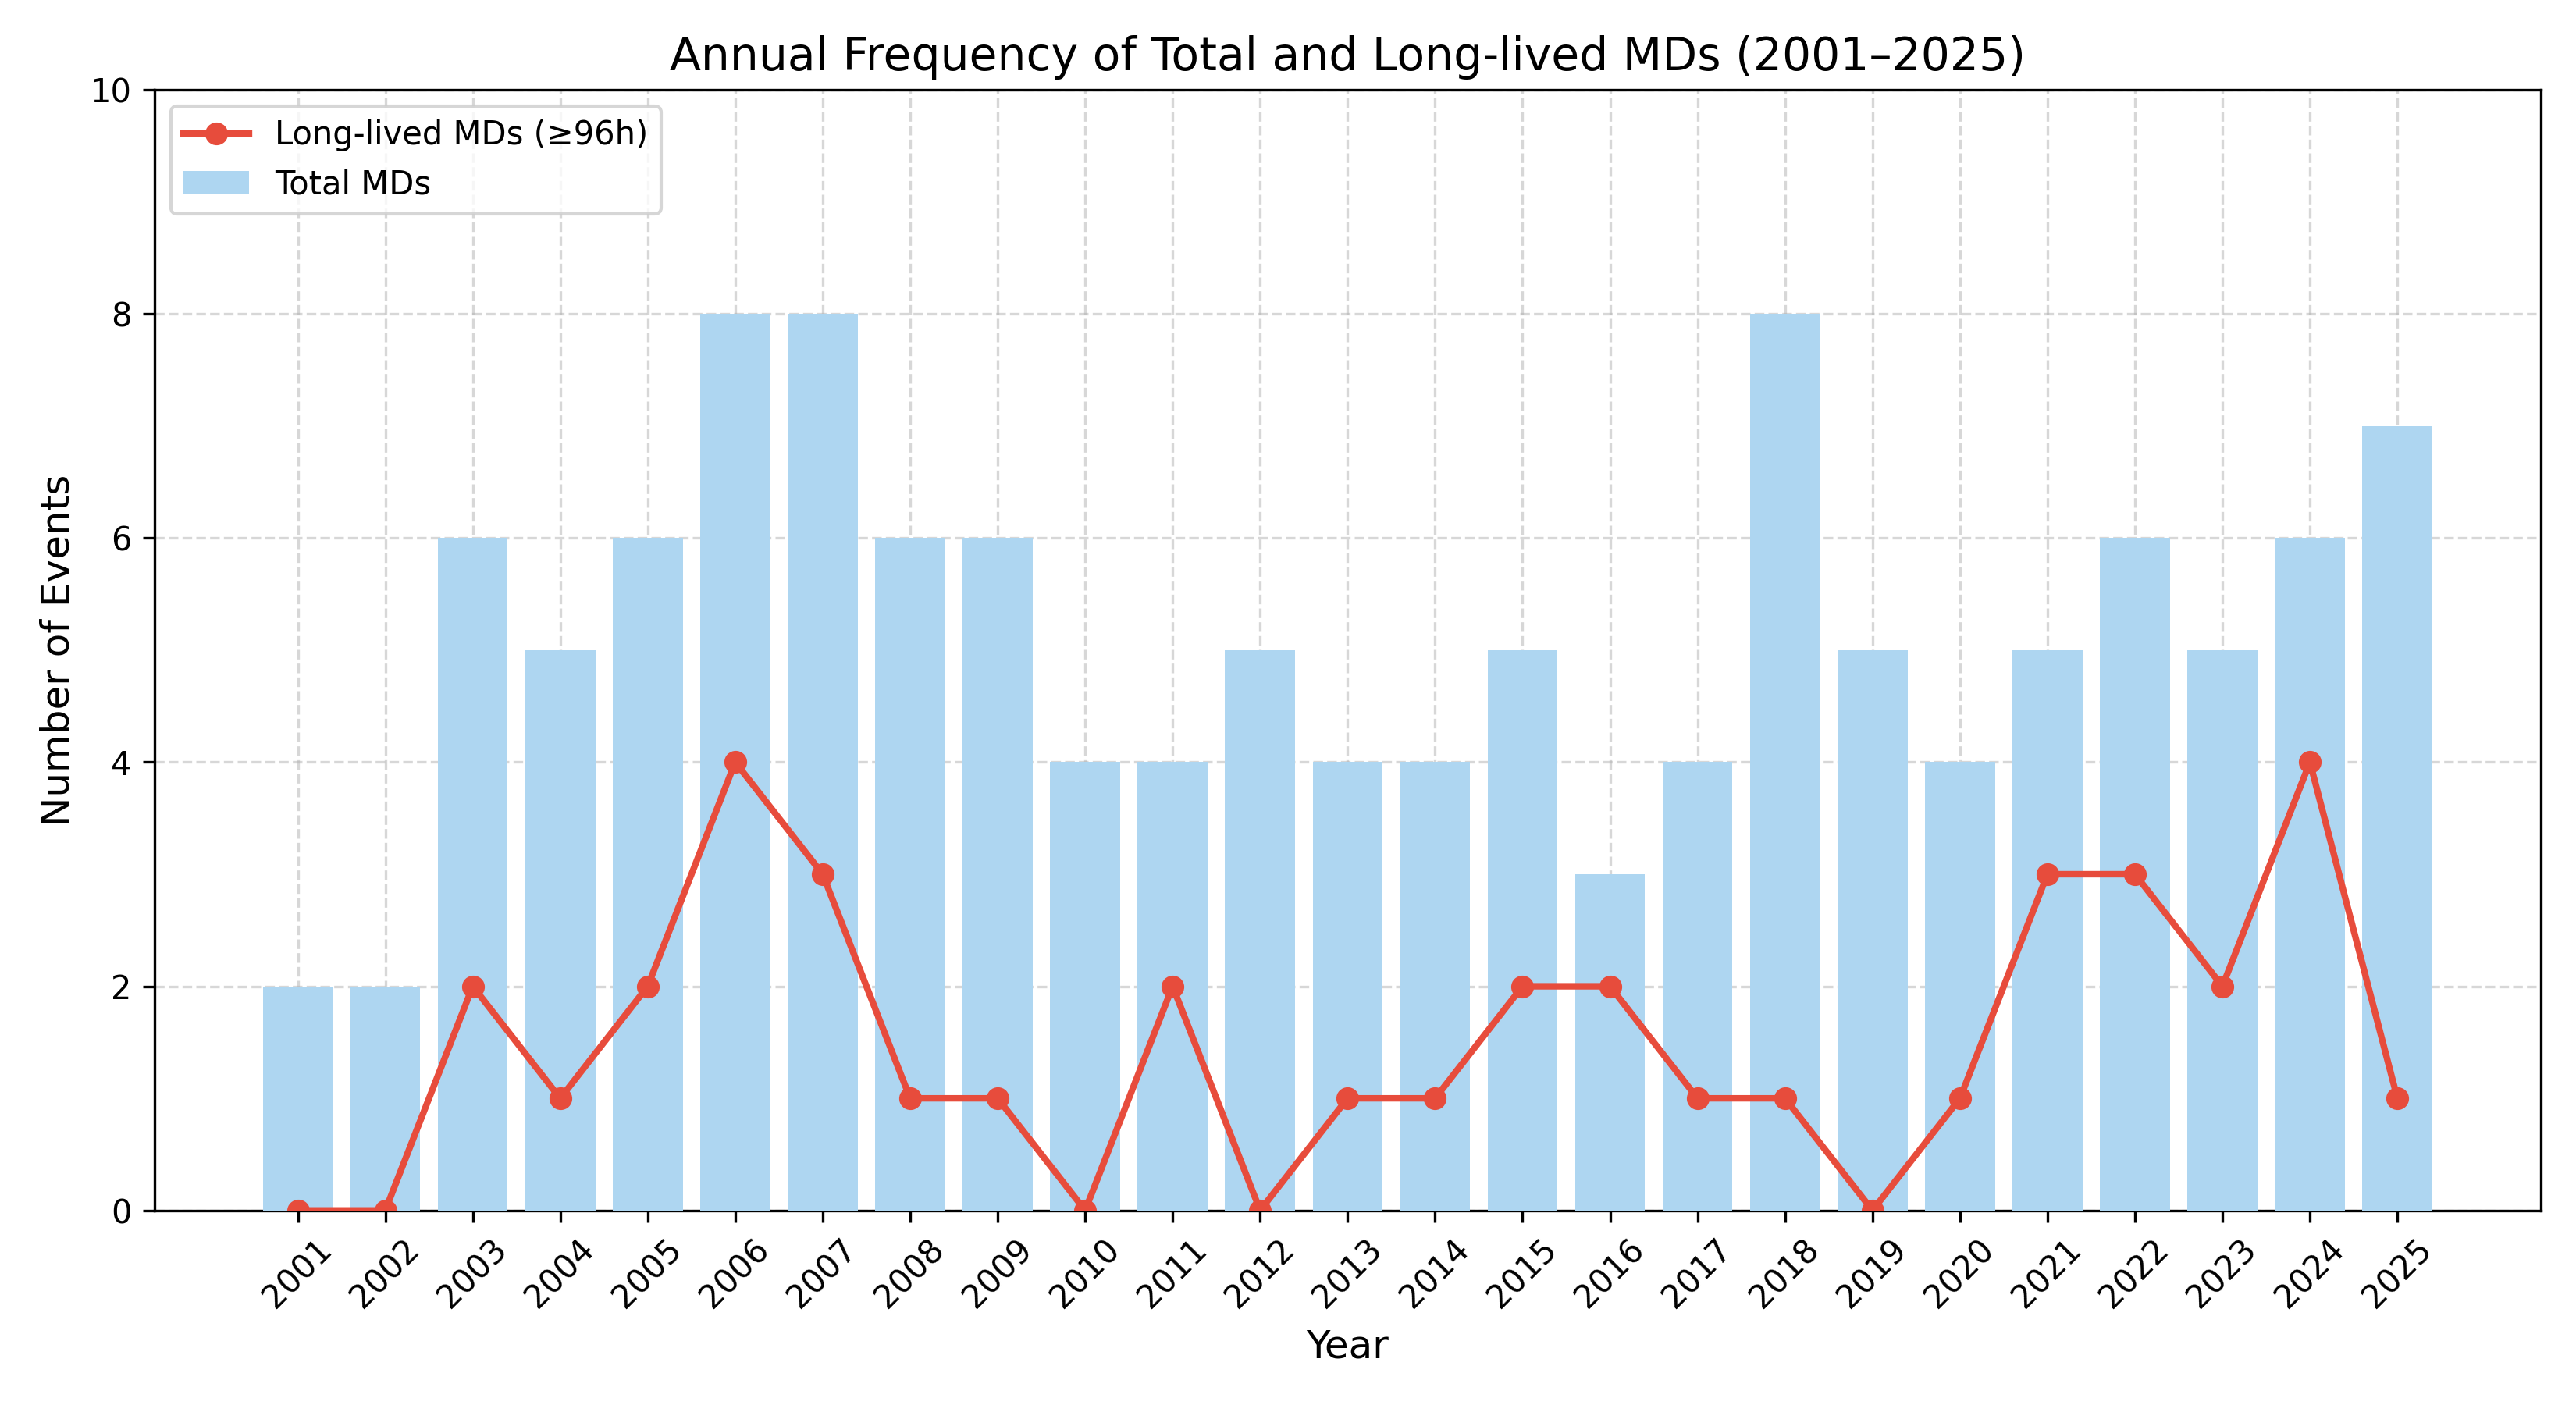
\includegraphics[width=0.86\textwidth]{annual_count_trend}
  \caption[Annual total and long-lived MD counts
  (2001--2025)]{Comparison of total annual MD frequency and the count
    of long-lived systems. The convergence of the line toward the top
  of the bars in years like 2016 indicates high longevity efficiency.}
  \label{fig:annual_md_count}
\end{figure}

The distribution of track durations
(Figure~\ref{fig:duration_histogram}) follows a right-skewed profile.
The ``long-tail'' representing systems surviving $\geq 96$\,h accounts
for approximately \textbf{31\%} of the total population (40 of 128 events).
The fact that this tail does not expand linearly with the total count
suggests that longevity is governed by the state of the land surface
(the BOE) rather than just the frequency of storm genesis.

\begin{figure}[H]
  \centering
  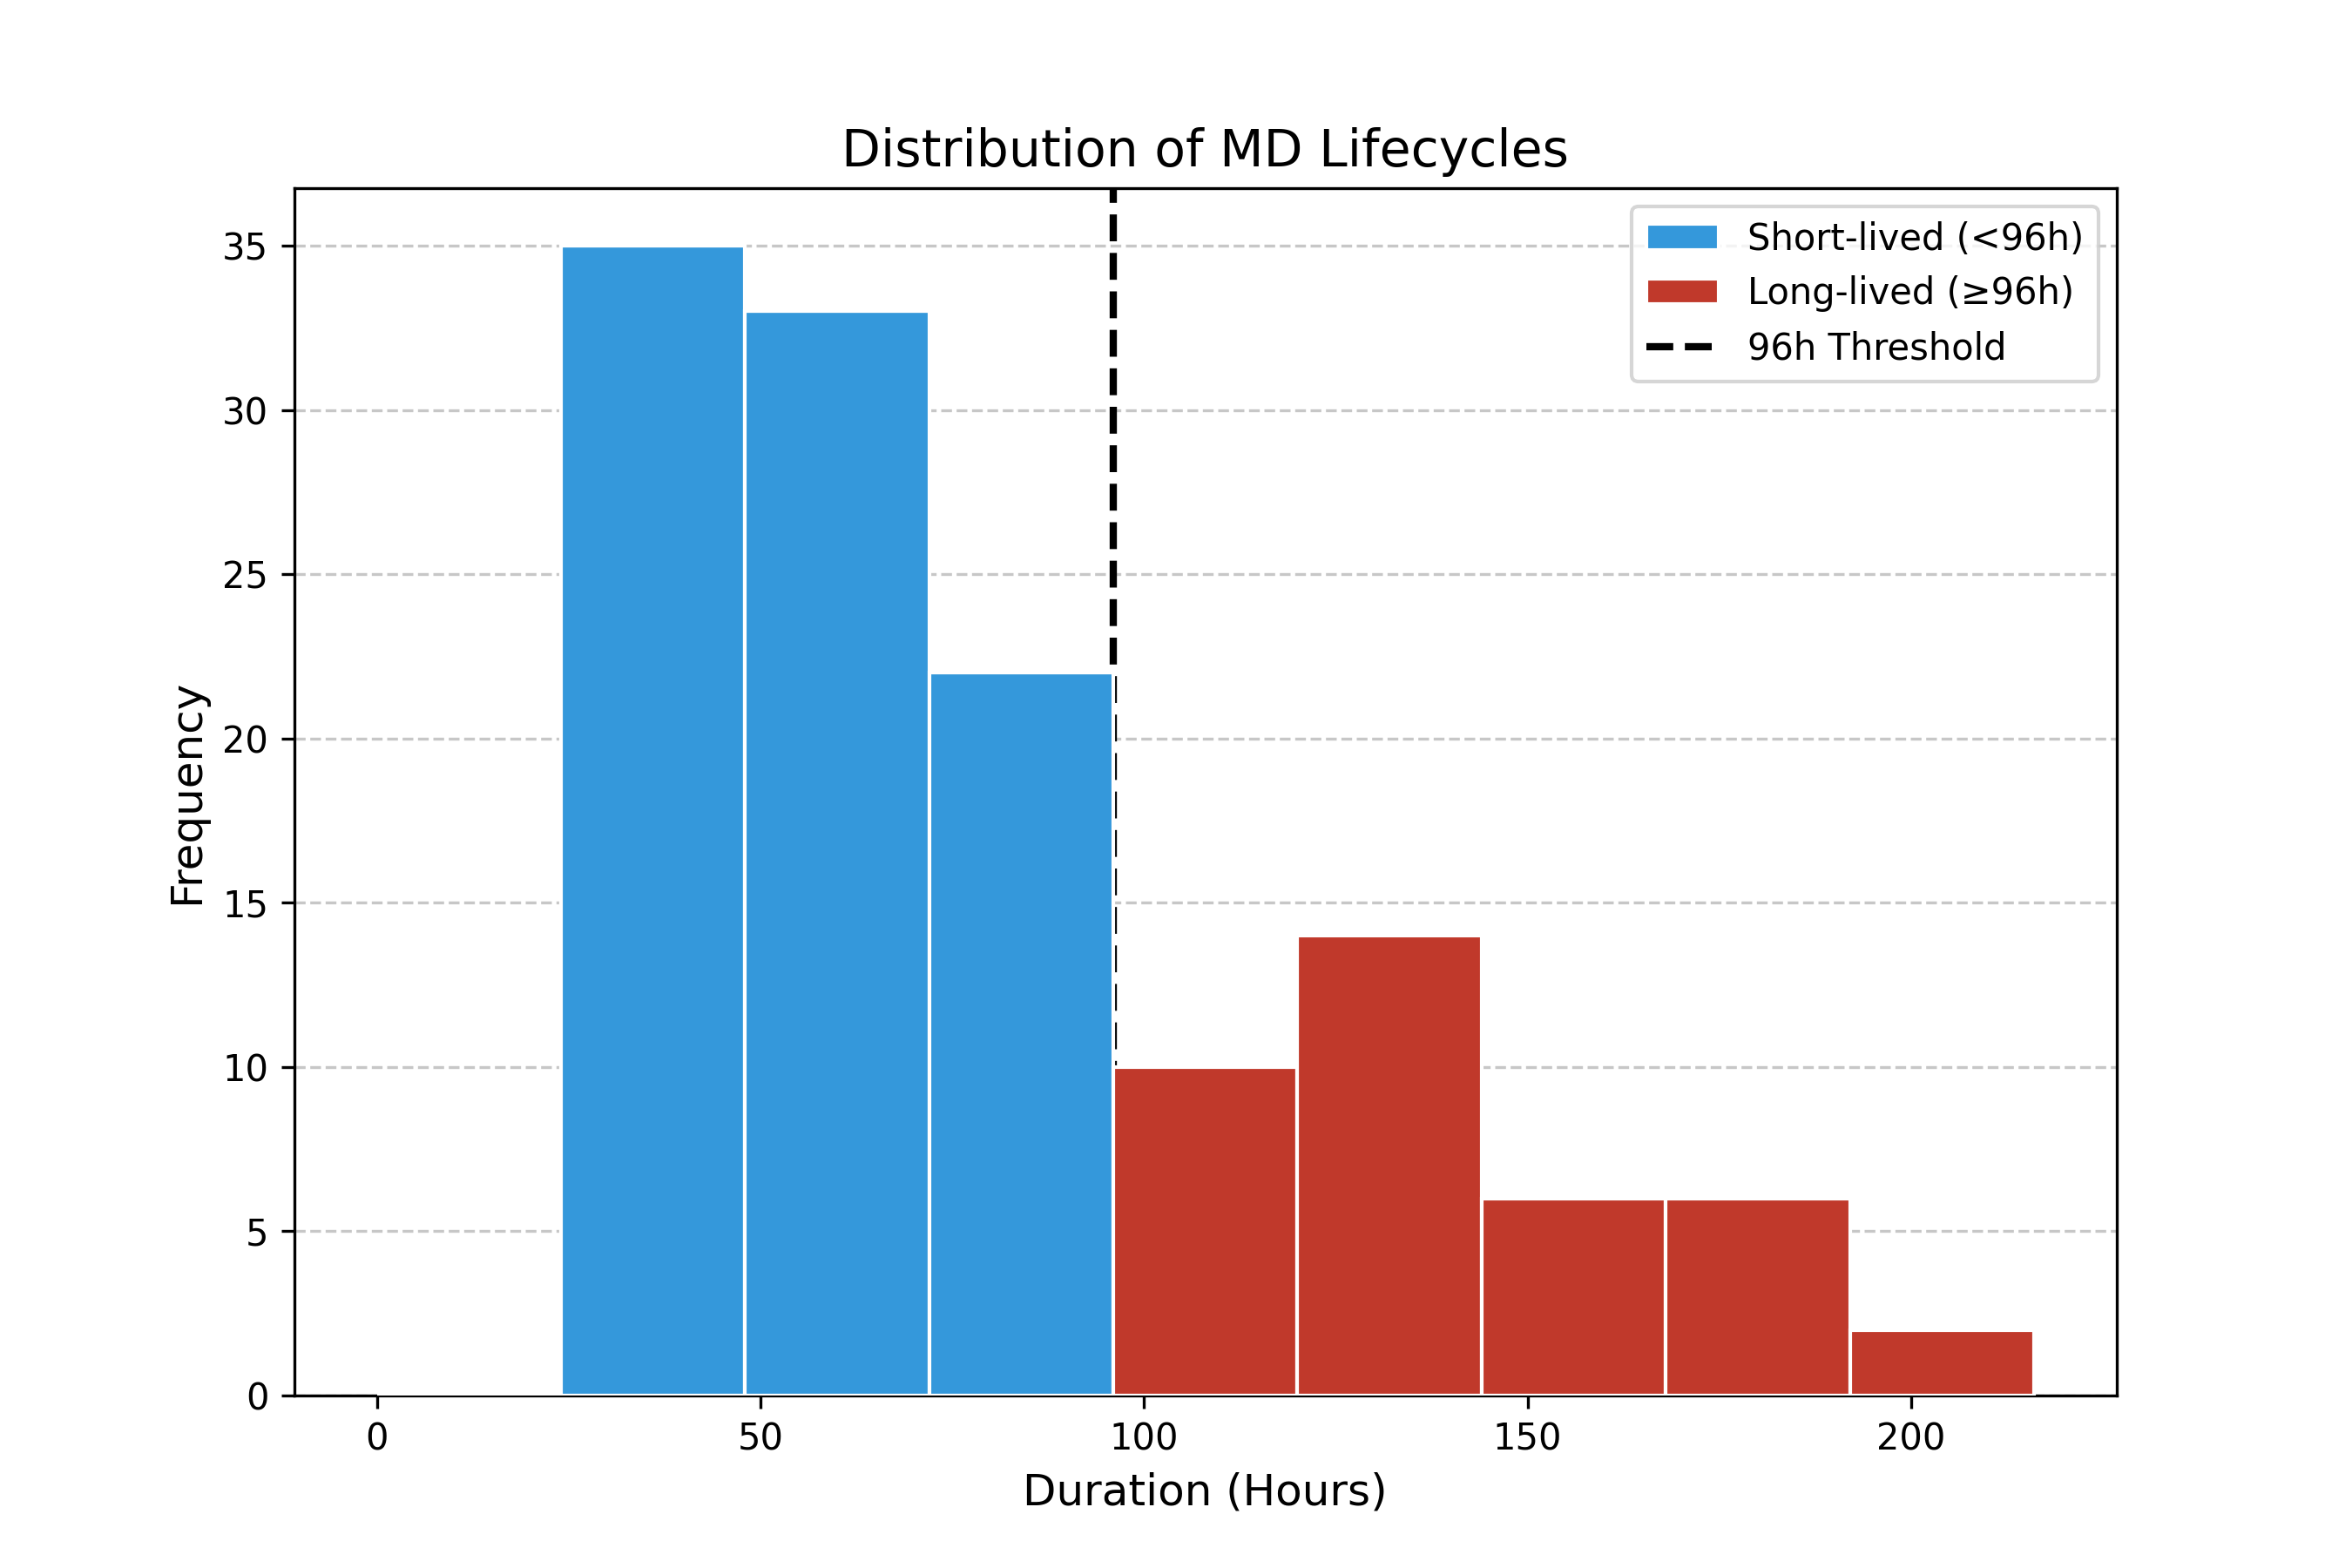
\includegraphics[width=0.75\textwidth]{duration_histogram}
  \caption[MD duration frequency distribution]{Histogram of track
    durations in 24-hour bins. The threshold at 96\,h separates
    short-lived (blue) from long-lived (red) systems, highlighting the
  BOE-sustained population.}
  \label{fig:duration_histogram}
\end{figure}

\subsection{Track Spatial Distribution}
\label{subsec:track_spatial}

Figure~\ref{fig:all_years_track_elevation} shows short-lived systems
predominantly terminate within 200--400\,km of the coastline, east of
the Eastern Ghats 600\,m contour. This spatial clustering is
consistent with terrain-induced structural disruption preventing
further inland transit in systems without an adequate surface energy
source. Long-lived systems extend well west of the Ghats into the
Gangetic plain, Madhya Pradesh and Maharasthra, indicating successful
terrain traversal. The spatial clustering of long-lived tracks over
the Gangetic plain corresponds closely to the region of highest
climatological July-August \texttt{swvl1} ($>0.3$\,m$^3$\,m$^{-3}$),
broadly consistent with the BOE hypothesis.

\textbf{Ocean-originated vs. land-genesis tracks :} Of the
\textbf{128} total events, \textbf{96.8\%} (124 events) originated
over the Bay of Bengal and made landfall along the eastern coast,
while only \textbf{3.2\%} (4 Land MDs) formed over the land surface
directly. This highlights that the vast majority of the MD population
relies on an initial oceanic moisture supply. Ocean-originated tracks
show a distinctly different thermodynamic evolution: they arrive at
the coast with well-organised vorticity, a sustained outer rainband,
and inner-core LHF of 100-150\,W\,m$^{-2}$ built up over 1-3 days
of oceanic energy supply.

This strong energetic initial condition means that even moderately
moist antecedent soils ($\texttt{swvl1} \approx 0.28$--$0.32$
\,m$^3$\,m$^{-3}$) may be sufficient to sustain the BOE in these
systems, since the MD arrives at the coast in a more intensified
state and the transition timescale to land-phase dependence is
longer. Land-originated systems, lacking this oceanic spin-up phase,
tend to be shorter-lived unless they form over a region of
anomalously high soil moisture.

\begin{figure}[H]
  \centering
  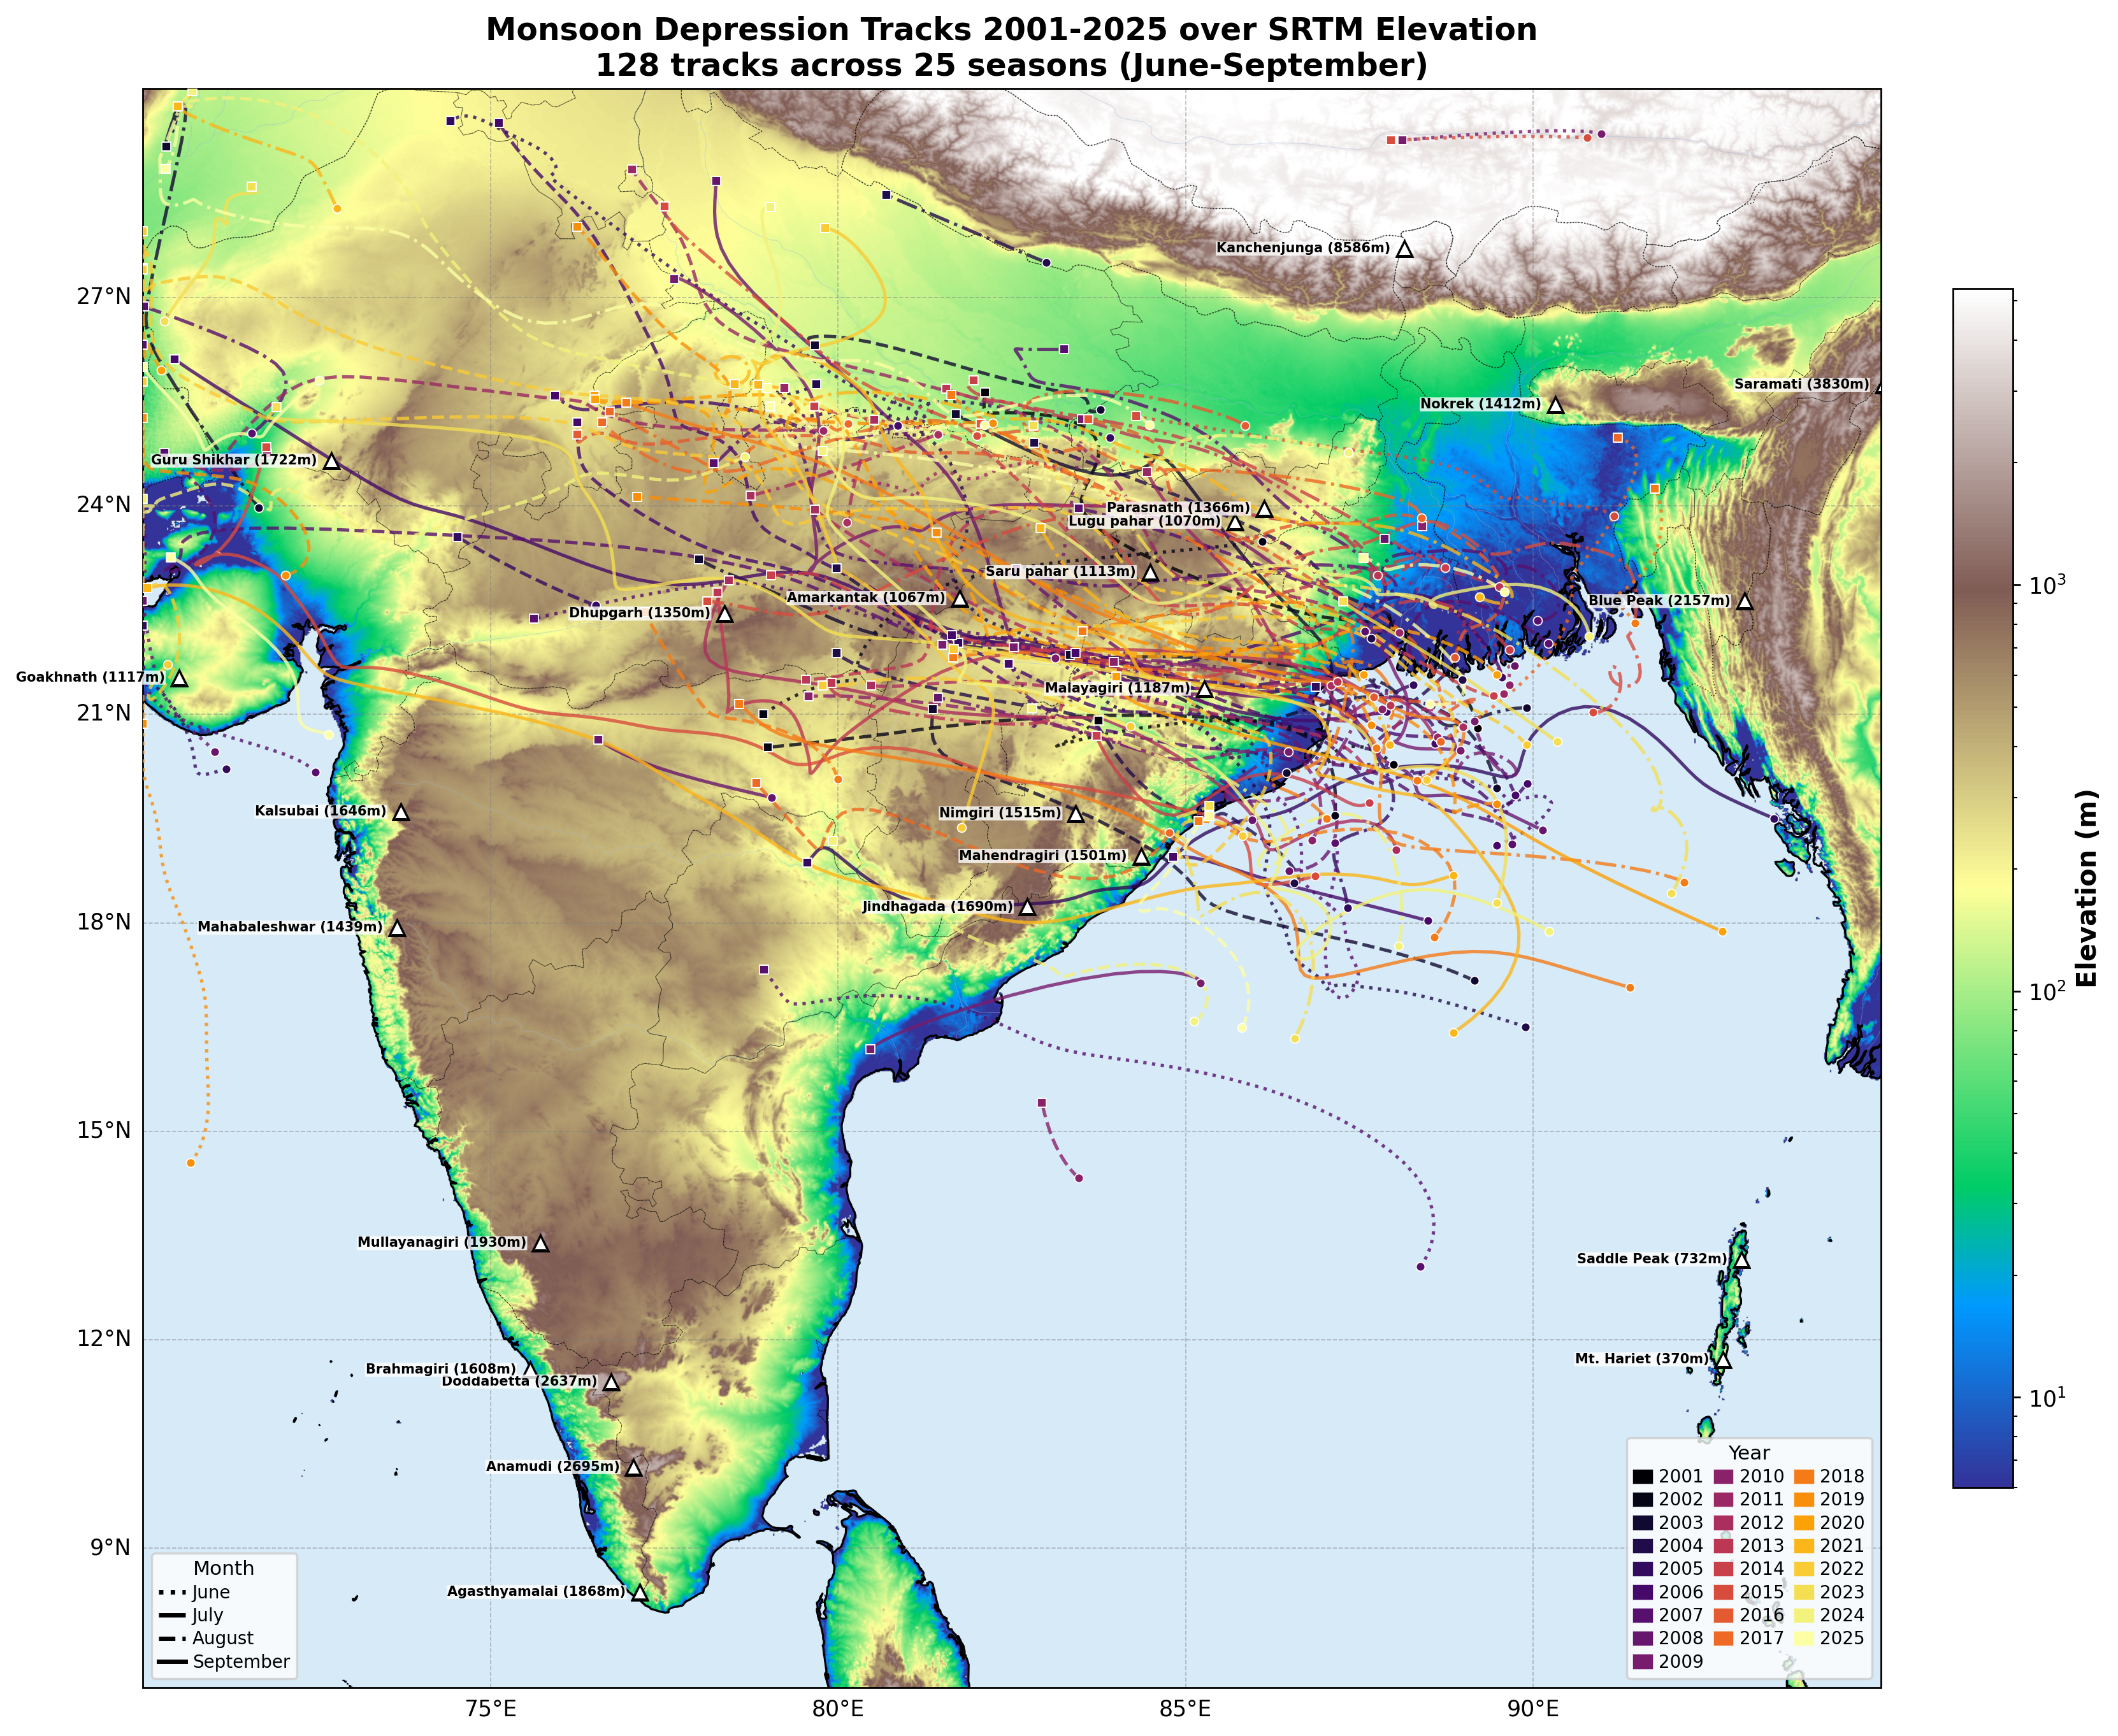
\includegraphics[width=0.92\textwidth]{all_years_tracks_elevation.png}
  \caption[Spatial distribution of MD tracks by duration
  category]{All confirmed MD tracks (2001--2025) coloured by
    duration; Eastern Ghats 600\,m contour overlaid. Landfall points
    marked by filled circles. Long-lived tracks cluster over the
  Gangetic plain west of the terrain.}
  \label{fig:all_years_track_elevation}
\end{figure}

% %%  FIGURE: All-track spatial map
% %%  SOURCE: Overall_years/MD_all_tracks_coloured_duration.png
% %%  Colour tracks by duration bins; add 600m Eastern Ghats contour;
% % mark landfall points.
% %%  Also overlay ERA5 July-August SWVL1 climatology as background
% % shading (optional).
% \begin{figure}[H]
%   \centering
%   \fbox{\rule{0pt}{7cm}\rule{0.90\textwidth}{0pt}}
%   % \includegraphics[width=0.90\textwidth]{all_md_tracks_coloured}
%   \caption[Spatial distribution of MD tracks by duration
%   category]{All confirmed MD tracks (2001-2025) coloured by
% duration; Eastern Ghats 600\,m contour (bold grey) overlaid.
% Landfall points marked by filled circles. Long-lived tracks cluster
% over the Gangetic plain west of the terrain.}
%   \label{fig:all_md_tracks_results}
% \end{figure}

\subsection{Annual MD Count and BOE Frequency}
\label{subsec:multiyear_count}

% Figure~\ref{fig:annual_md_count_boe_fraction} displays the annual
% frequency of MDs alongside the fraction of systems meeting the BOE
% candidacy criteria ($\geq 70$,W,m$^{-2}$ LHF for $\geq 18$,h).

Two primary observations emerge from the climatology:
\begin{enumerate}
  \item \textbf{Stability of Genesis:} The total annual MD count
    shows no statistically significant monotonic trend ($p > 0.1$),
    consistent with the findings of \autocite{mishra2021monsoon}
    regarding stable synoptic frequency.
  \item \textbf{BOE Variability:} The BOE candidate fraction is
    substantially more variable year-to-year than the total count.
    This demonstrates that post-landfall persistence is not a simple
    function of genesis frequency, but is controlled by a state
    variable-land-surface moisture-that fluctuates independently of
    the large-scale atmospheric triggers for genesis.
\end{enumerate}

% \begin{figure}[H]
%   \centering
%   \includegraphics[width=0.88\textwidth]{Overall_years/annual_md_count_boe_fraction}
%   \caption{Annual MD count and BOE-candidate fraction over
%     2001--2025. The high interannual variability of the BOE fraction
%   suggests land-surface control over system longevity.}
%   \label{fig:annual_md_count_boe_fraction}
% \end{figure}

% \section{Azimuthal Hovm\"{o}ller Analysis}
\section{Azimuthal Hovm\texorpdfstring{\"{o}}{o}ller Analysis}
\label{sec:results_hovmoller}

While the climatological overview established the frequency of inland
penetration, this section identifies the physical mechanisms governing
that sustainability through an azimuthal perspective. By transforming the
MD into a storm-centered radial coordinate system, we can isolate the
evolution of the inner-core thermodynamics, where the BOE feedback is most
important, from the surrounding large-scale monsoon flow. Therefore we
identify the radial-temporal signature of the BOE by comparing the evolution
of long-lived (BOE-active) and short-lived (Non-BOE) MDs across the 2001–2025
period that govern inland sustainability. % By centering the analysis on
% landfall ($t=0$), we isolate the transition from oceanic to terrestrial
% energy dependence.

The analysis is centered on the moment of landfall ($t=0$) to capture
the critical transition from oceanic to terrestrial energy
dependence. To contrast the differing regimes, we examine two
representative cases from the 2001–2025 database:
\begin{itemize}
  \item \textbf{BOE-Active (Long-lived):} Track 5 from September 2024
    (6th to 12th September), which successfully navigated the Eastern
    Ghats and penetrated deep into the Indian heartland.
  \item \textbf{Non-BOE (Short-lived):} A June 2001 system (11th to
    14th June) that underwent rapid structural collapse shortly after landfall.
\end{itemize}

% --- BOE-ACTIVE SYSTEM ---
\begin{figure}[H]
  \centering
  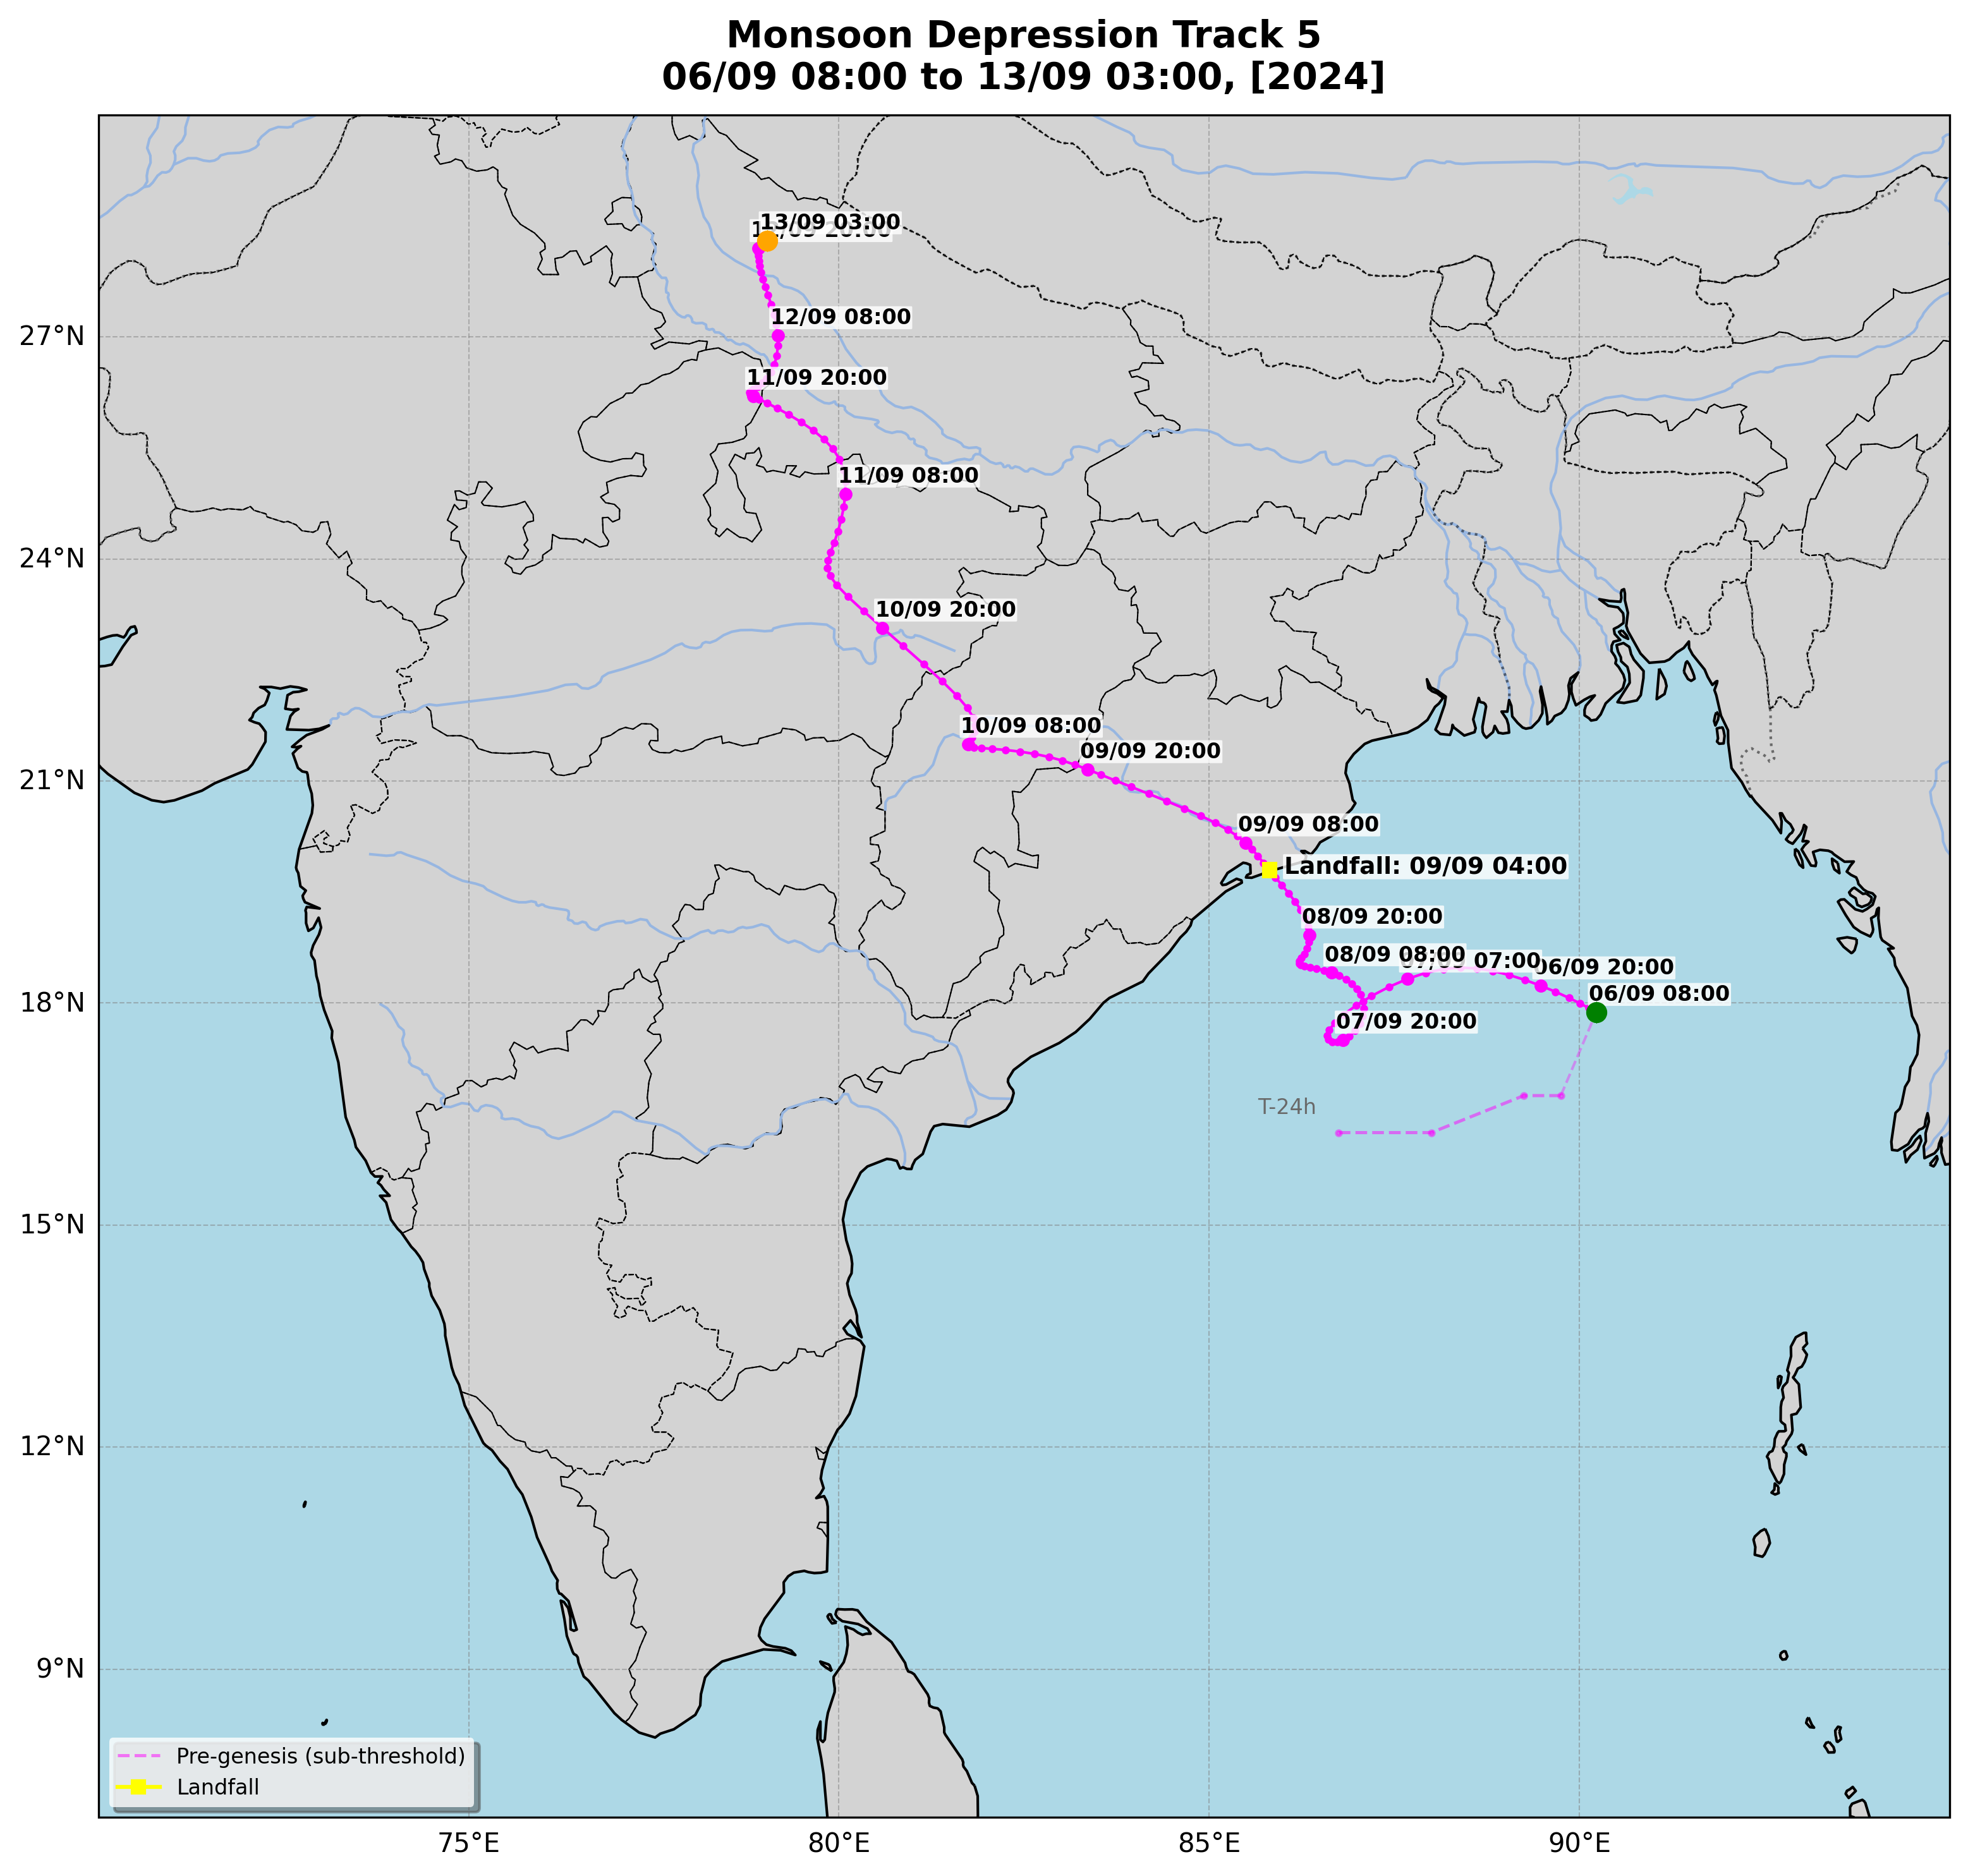
\includegraphics[width=0.67\textwidth]{track_long_spatial}
  \caption{Long-lived Track (Sept 2024), BOE Track Path}
  \label{fig:tp_long_spatial}
\end{figure}

% --- NON-BOE SYSTEM ---
\begin{figure}[H]
  \centering
  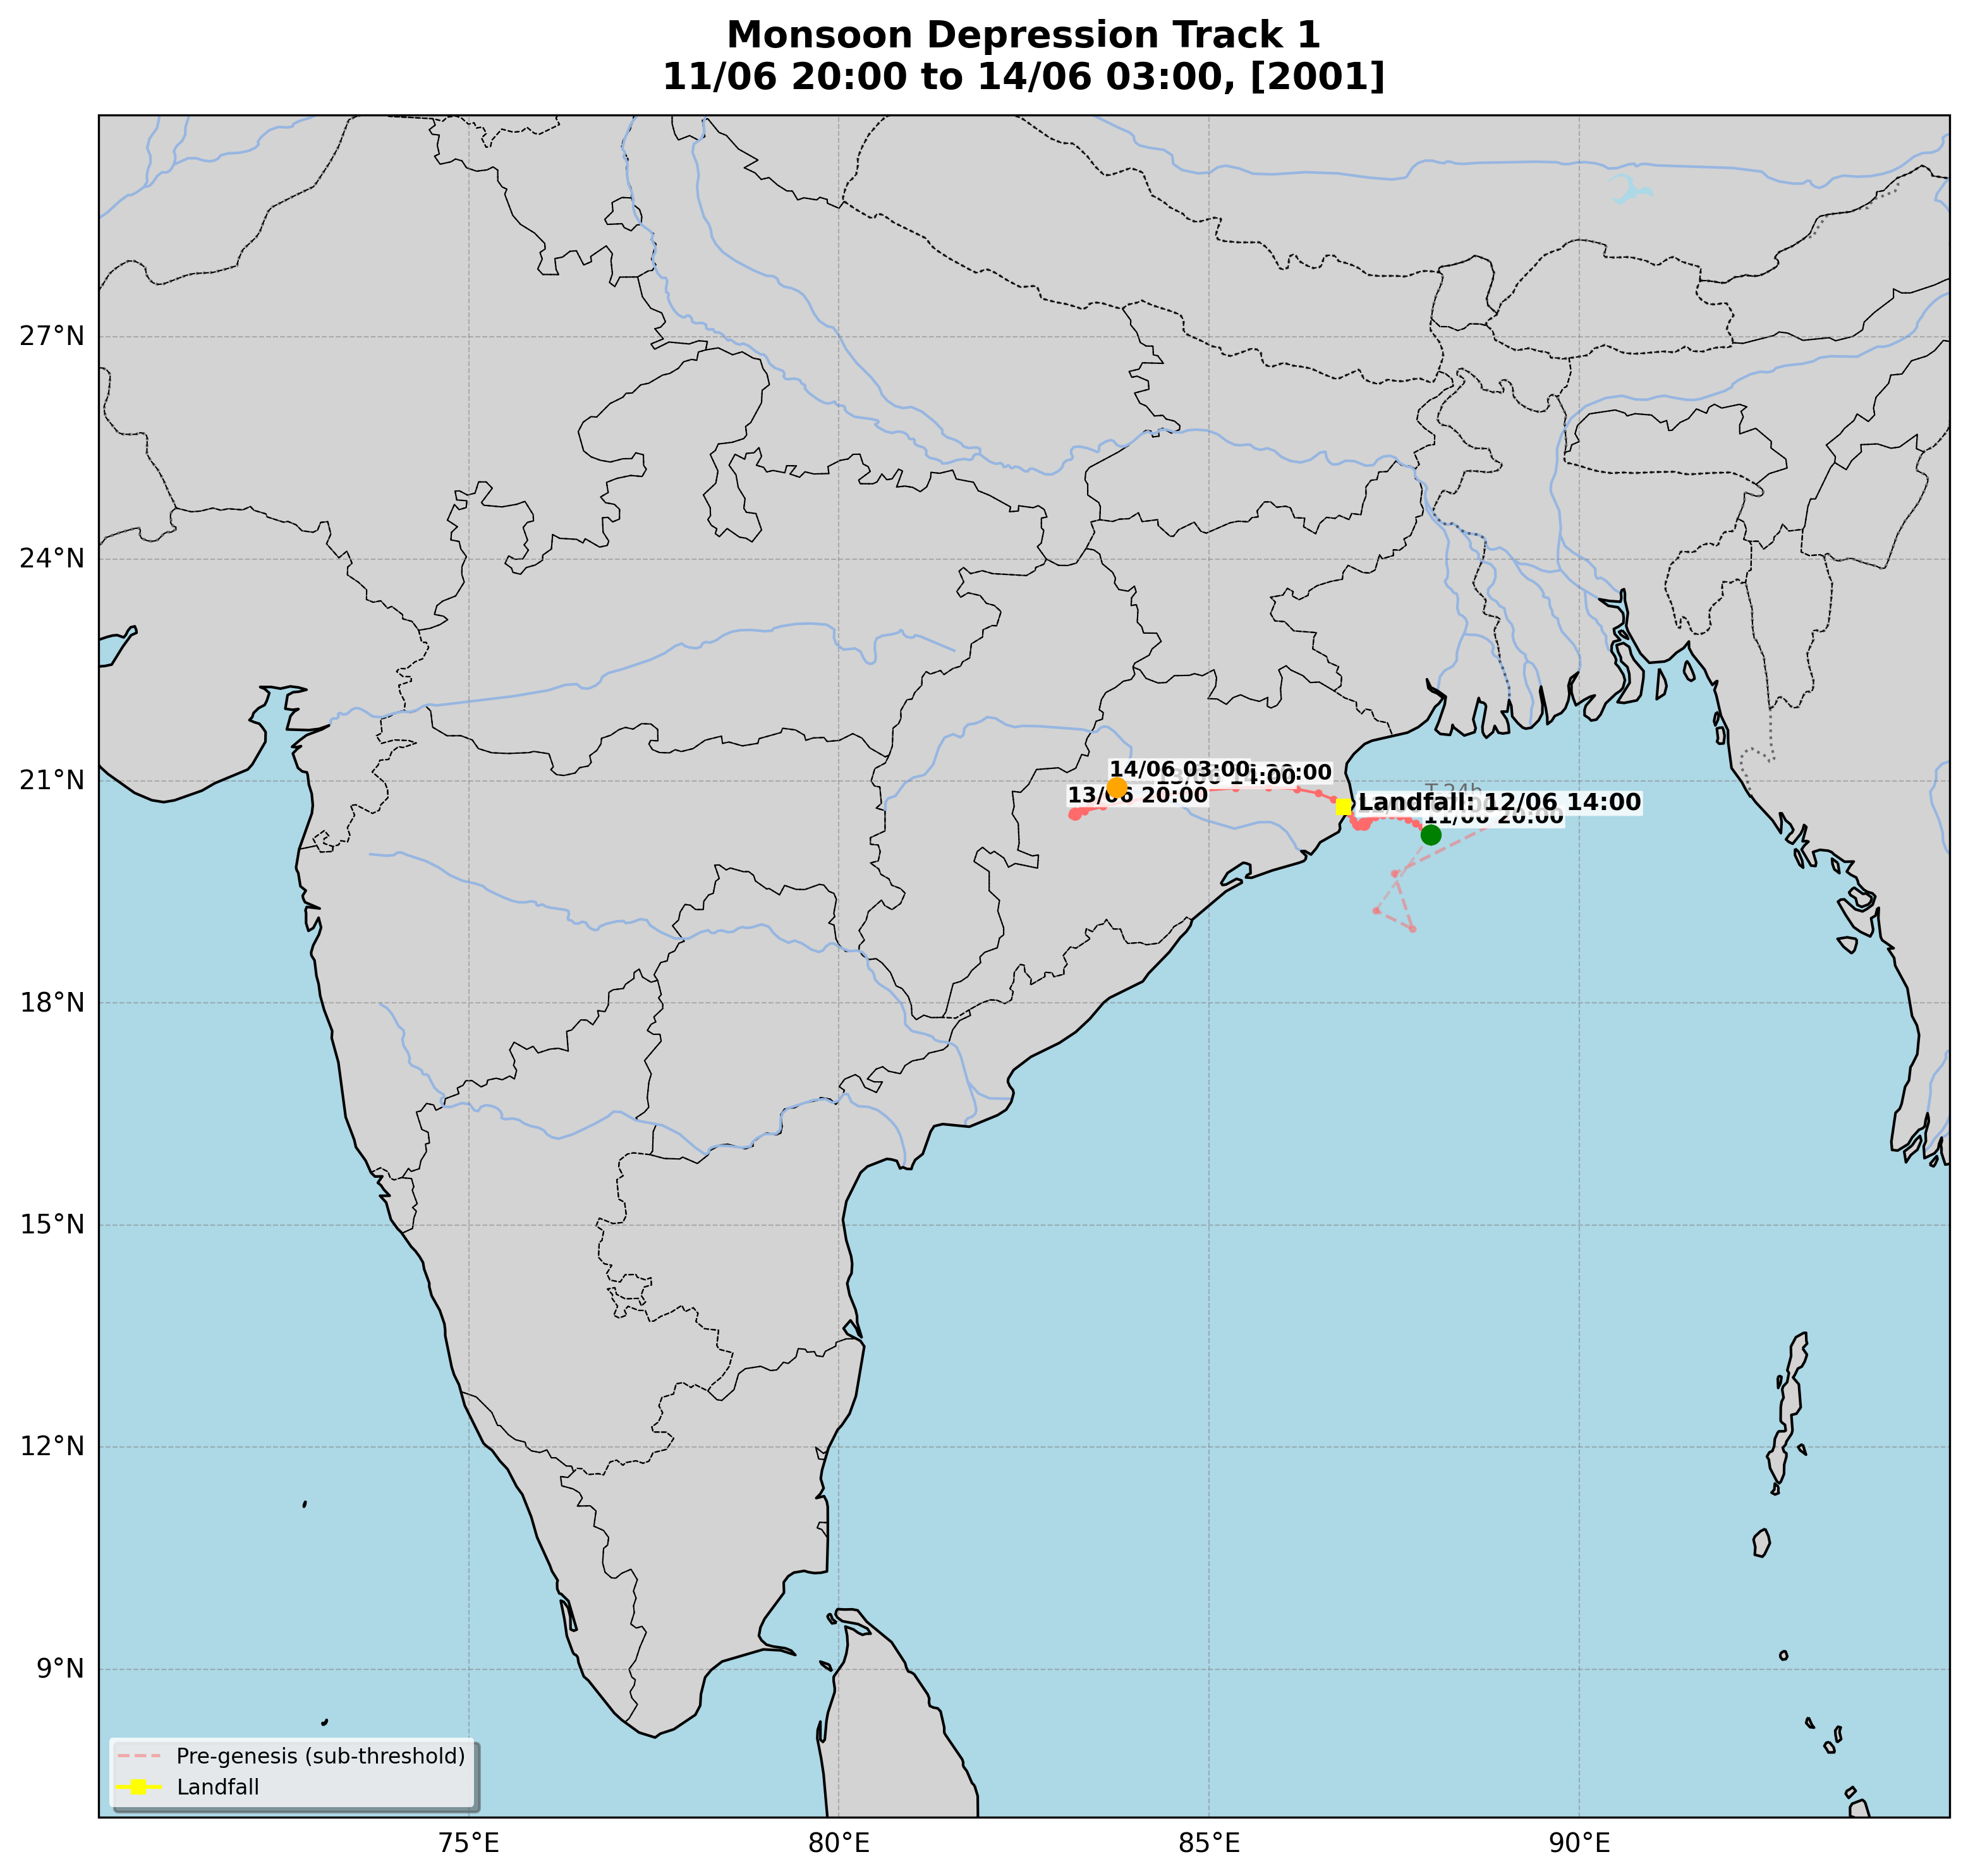
\includegraphics[width=0.67\textwidth]{track_short_spatial}
  \caption{Short-lived Track (June 2001), Non-BOE Track Path}
  \label{fig:tp_short_spatial}
\end{figure}

The above spatial track paths for the representative systems used in
the azimuthal analysis. The long-lived system exhibits a sustained
westward trajectory, whereas the short-lived system terminates on the
windward slopes of the terrain.

\subsection{Total Precipitation Dynamics}
\label{subsec:hovmoller_tp}

The evolution of total precipitation (\texttt{TP}) provides the most
visible evidence of the BOE mechanism. As shown in the representative
long-lived case, corresponding hovm\"oller plot
(Figure~\ref{fig:hovmoller_tp_long}), the MD
undergoes a structural regime shift.

In contrast, short-lived systems, corresponding hovm\"oller plot
(Figure~\ref{fig:hovmoller_tp_short}), exhibit a uniform radial
collapse. The absence of a sufficient land-surface energy source
leads to heavy precipitation at landfall leads to the simultaneous
dissipation of both core and peripheral convection within 24 hours of landfall.

\begin{figure}[H]
  \centering
  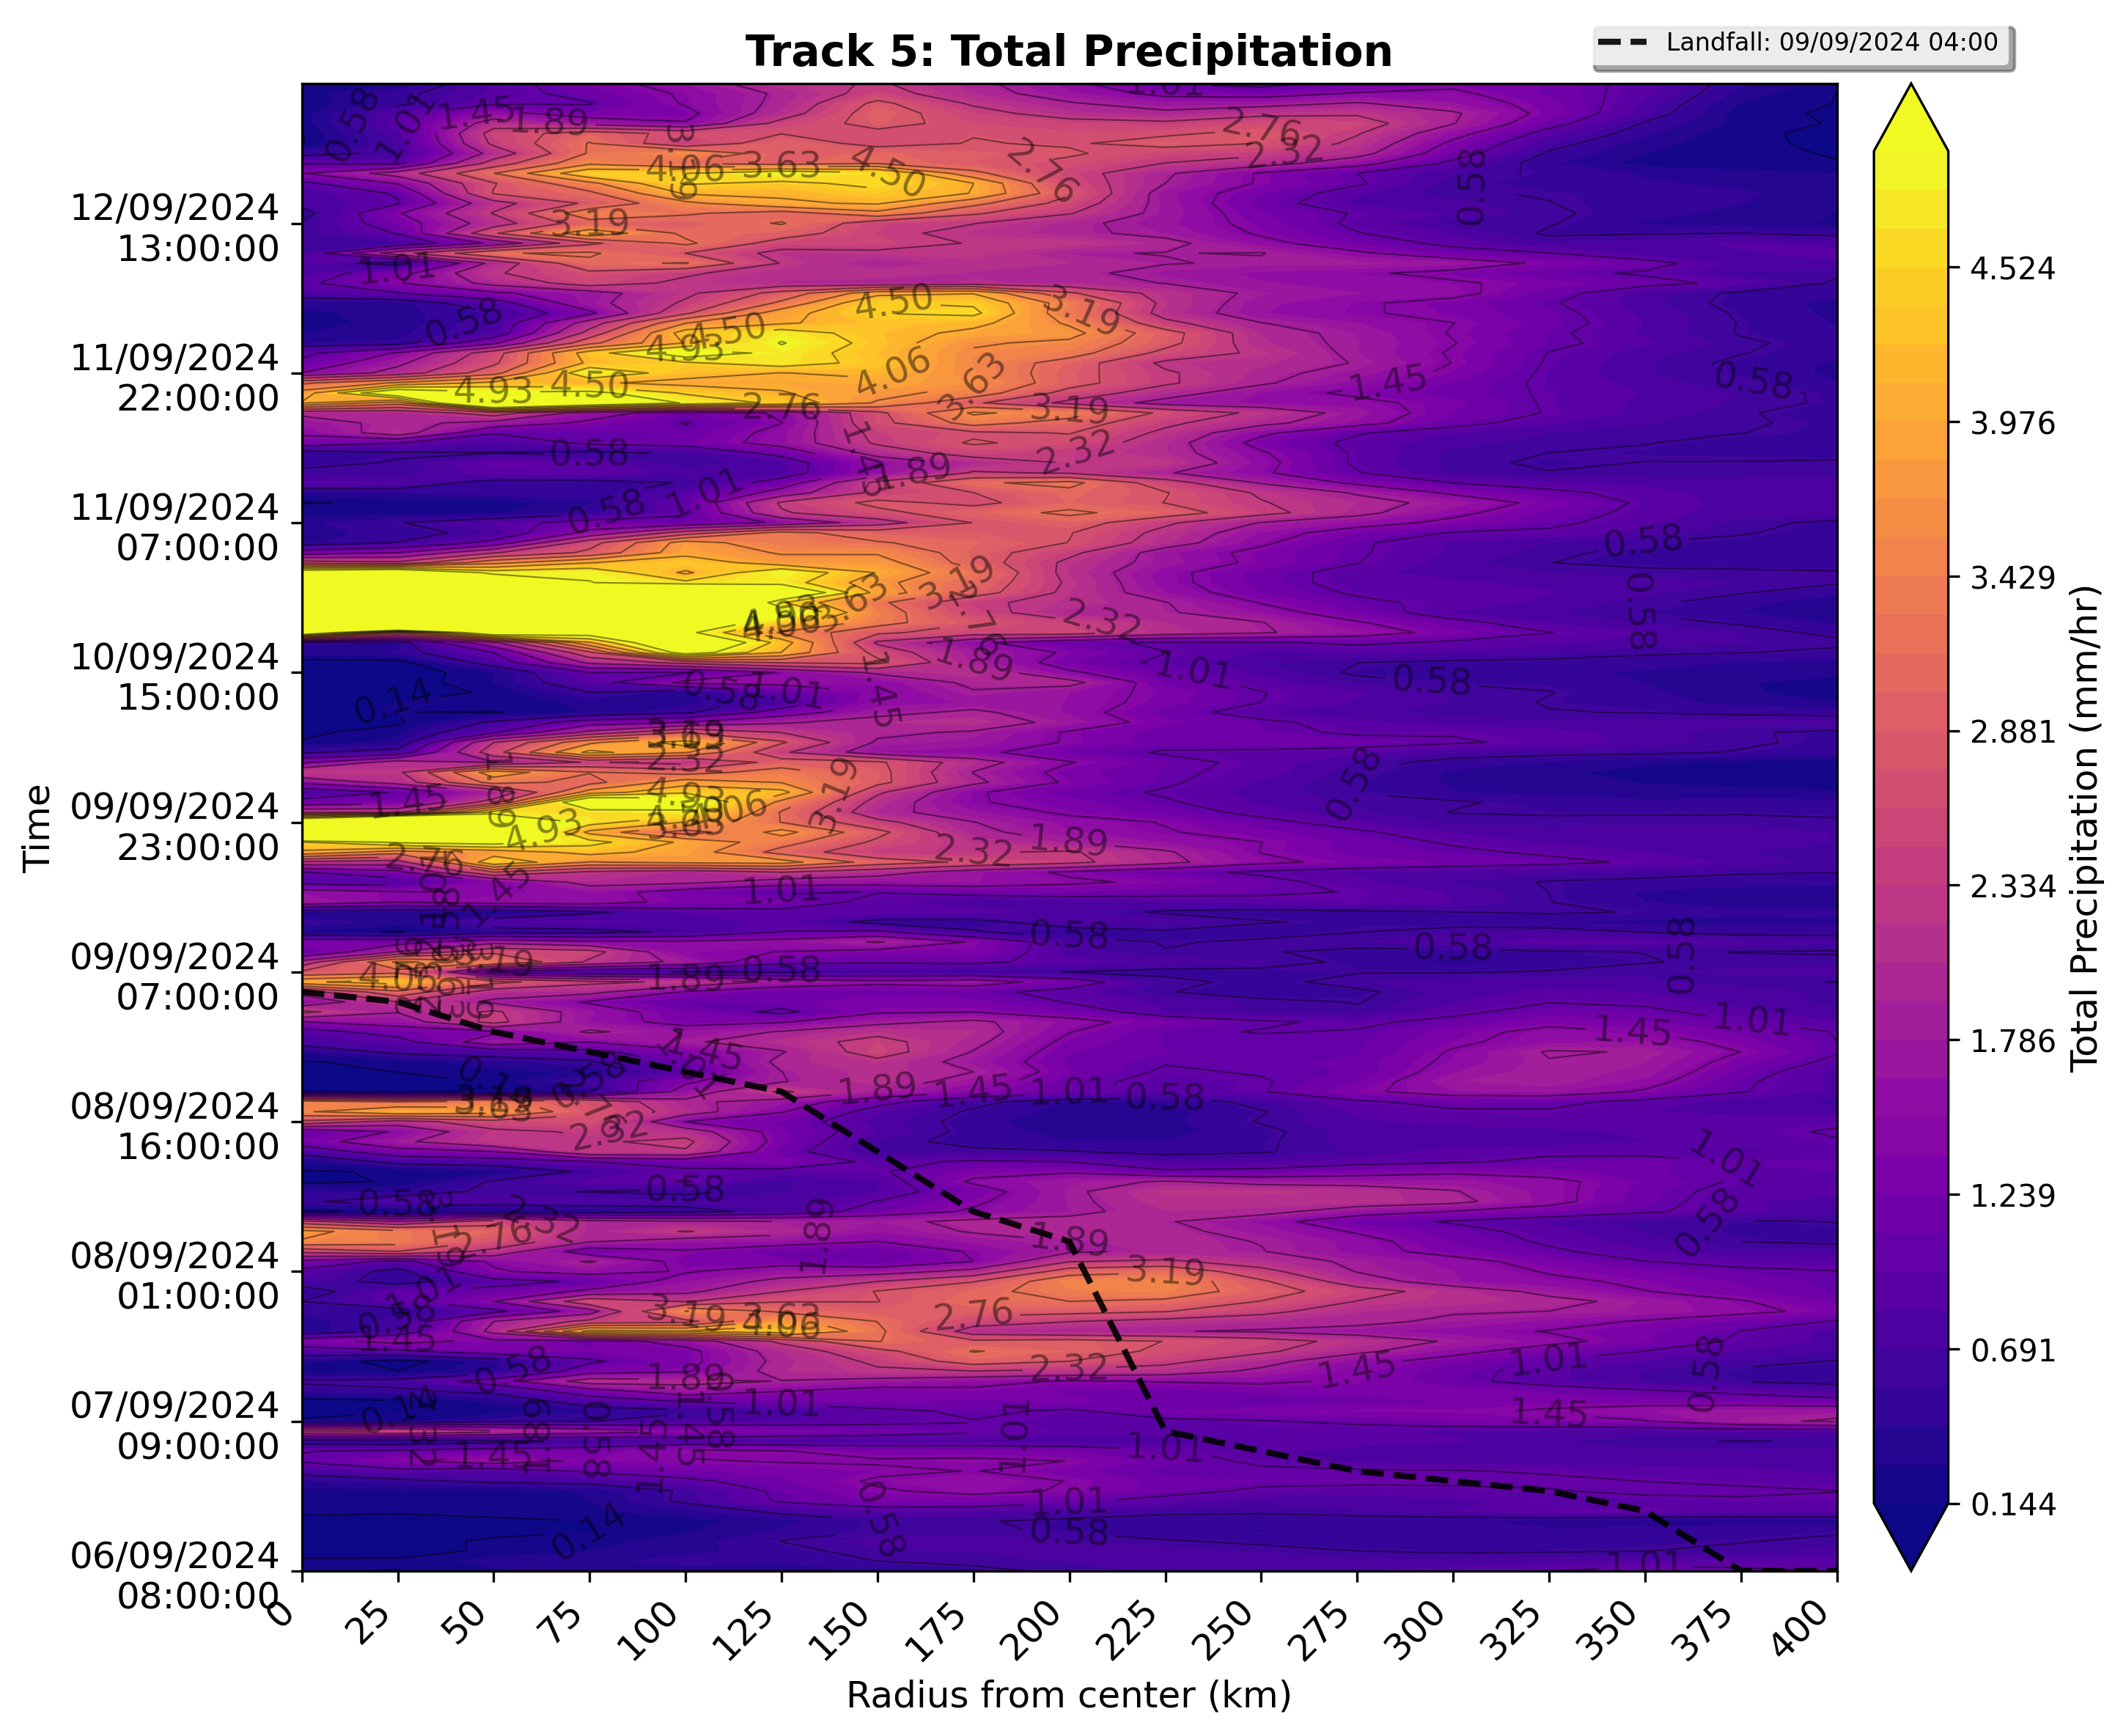
\includegraphics[width=0.69\textwidth]{track_long_tp_hov}
  \caption{Uniform precipitation after landfall}
  \label{fig:hovmoller_tp_long}
\end{figure}

\begin{figure}[H]
  \centering
  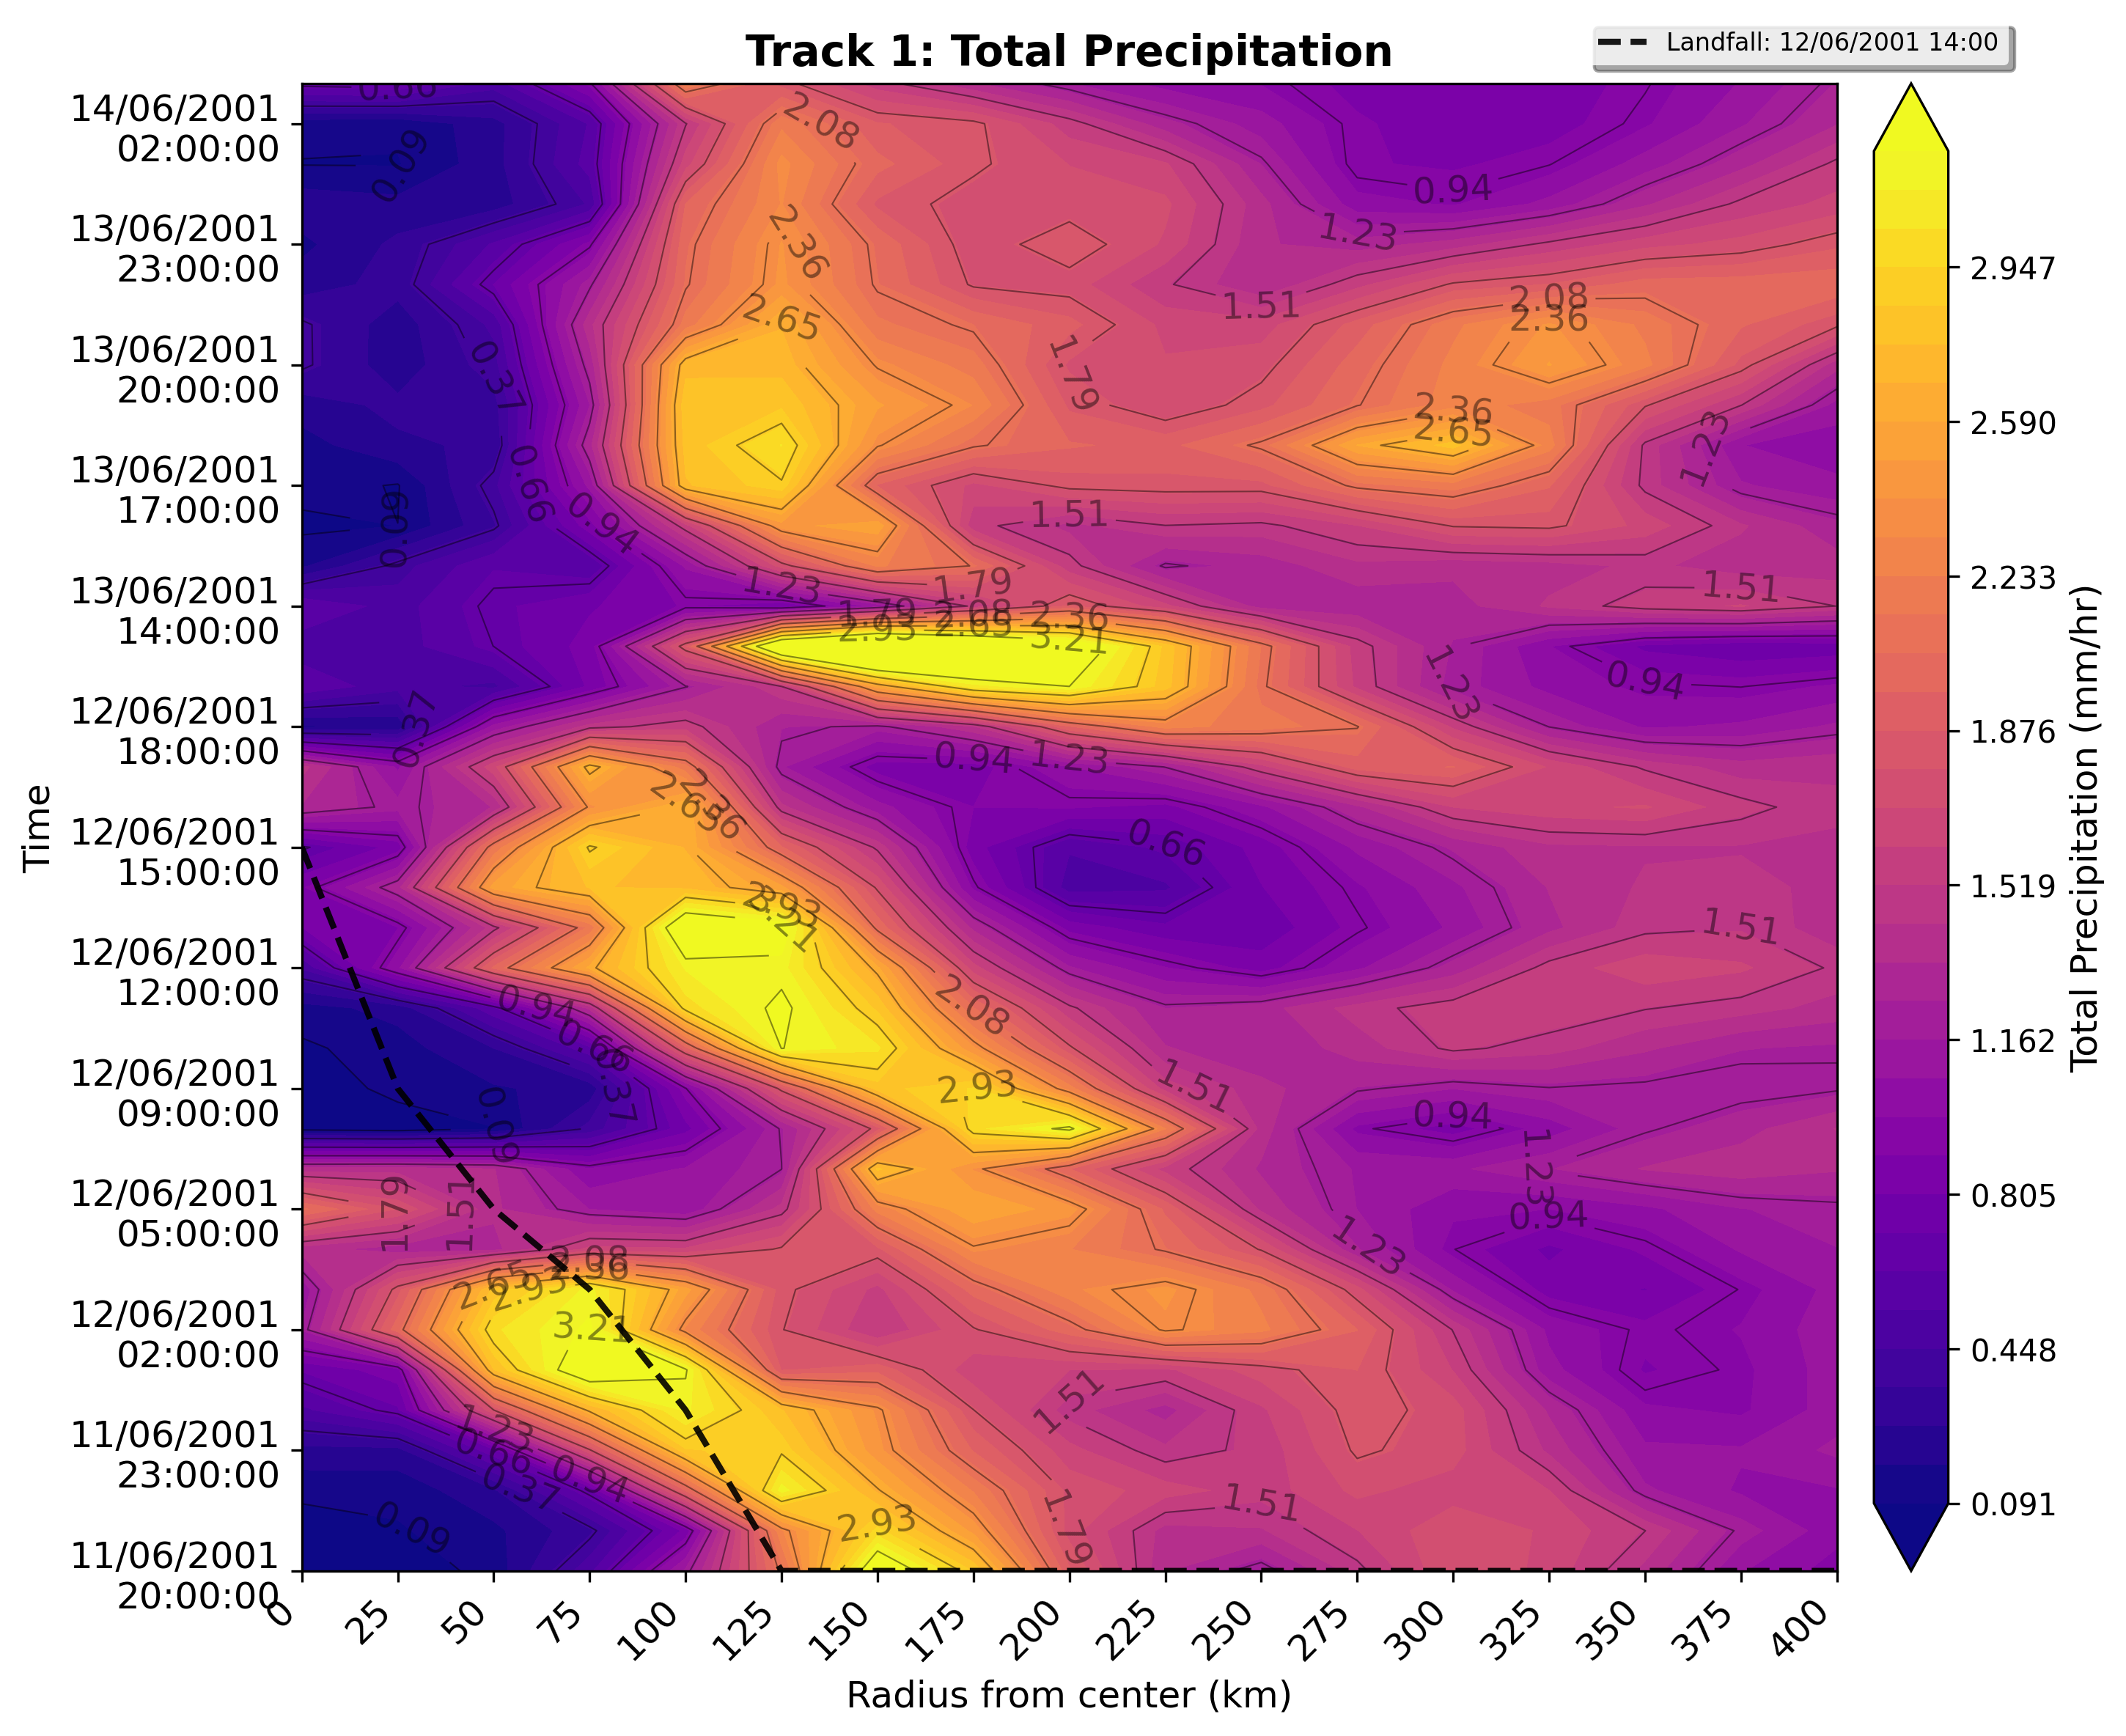
\includegraphics[width=0.69\textwidth]{track_short_tp_hov}
  \caption{Heavy precipitation at landfall}
  \label{fig:hovmoller_tp_short}
\end{figure}

% \caption{MD spatial track and Hovm\"{o}ller of precipitation. The
% long-lived system maintains its core rain-rate even after landfall.}
% \label{fig:hov_track_comparison_tp}

\subsection{Soil Moisture: Exposure Duration and Feedbacks}
\label{subsec:hovmoller_swvl1}

The Soil Water Volumetric level-1 (\texttt{SWVL1}) Hovm\"{o}ller
comparison (Figure~\ref{fig:hov_long_swvl1} and
\ref{fig:hov_short_swvl1}) reveals a critical temporal distinction in
surface energy availability. While both long-lived and short-lived
systems encounter similar absolute volumetric ranges (approximately
0.24-0.43\,m$^3$\,m$^{-3}$), their interaction with this moisture
reservoir differs in two key ways:

\textbf{Sustained Inland Exposure:} In the long-lived (BOE-active)
case (Figure~\ref{fig:hov_long_swvl1}), the system maintains
exposure to high soil moisture levels ($\gtrsim
0.38$\,m$^3$\,m$^{-3}$) for more than 72 hours post-landfall. This
extended exposure time with moist soil allows the system to continuously extract
latent heat as it traverses the Gangetic Plain.

\textbf{The Self-Wetting Signal:} Post-landfall ($t > 0$), the
long-lived MD displays a widening saturated core at radii
$<100$\,km. This is the evidence of a self-wetting feedback: the
storm's own precipitation replenishes the soil moisture,preventing
the rapid surface drying that typically follows landfall.

In contrast, while short-lived systems may encounter initially moist
soils (Figure~\ref{fig:hov_short_swvl1}) the duration of this
exposure is significantly truncated. Convective organization
collapses within 24 hours, often before the self-wetting feedback can
establish a stable energy-limited evaporation regime. This suggests
that the \textbf{persistence of the moist surface contact}, rather
than just the initial value, is the true gatekeeper of MD longevity.

\begin{figure}[H]
  \centering
  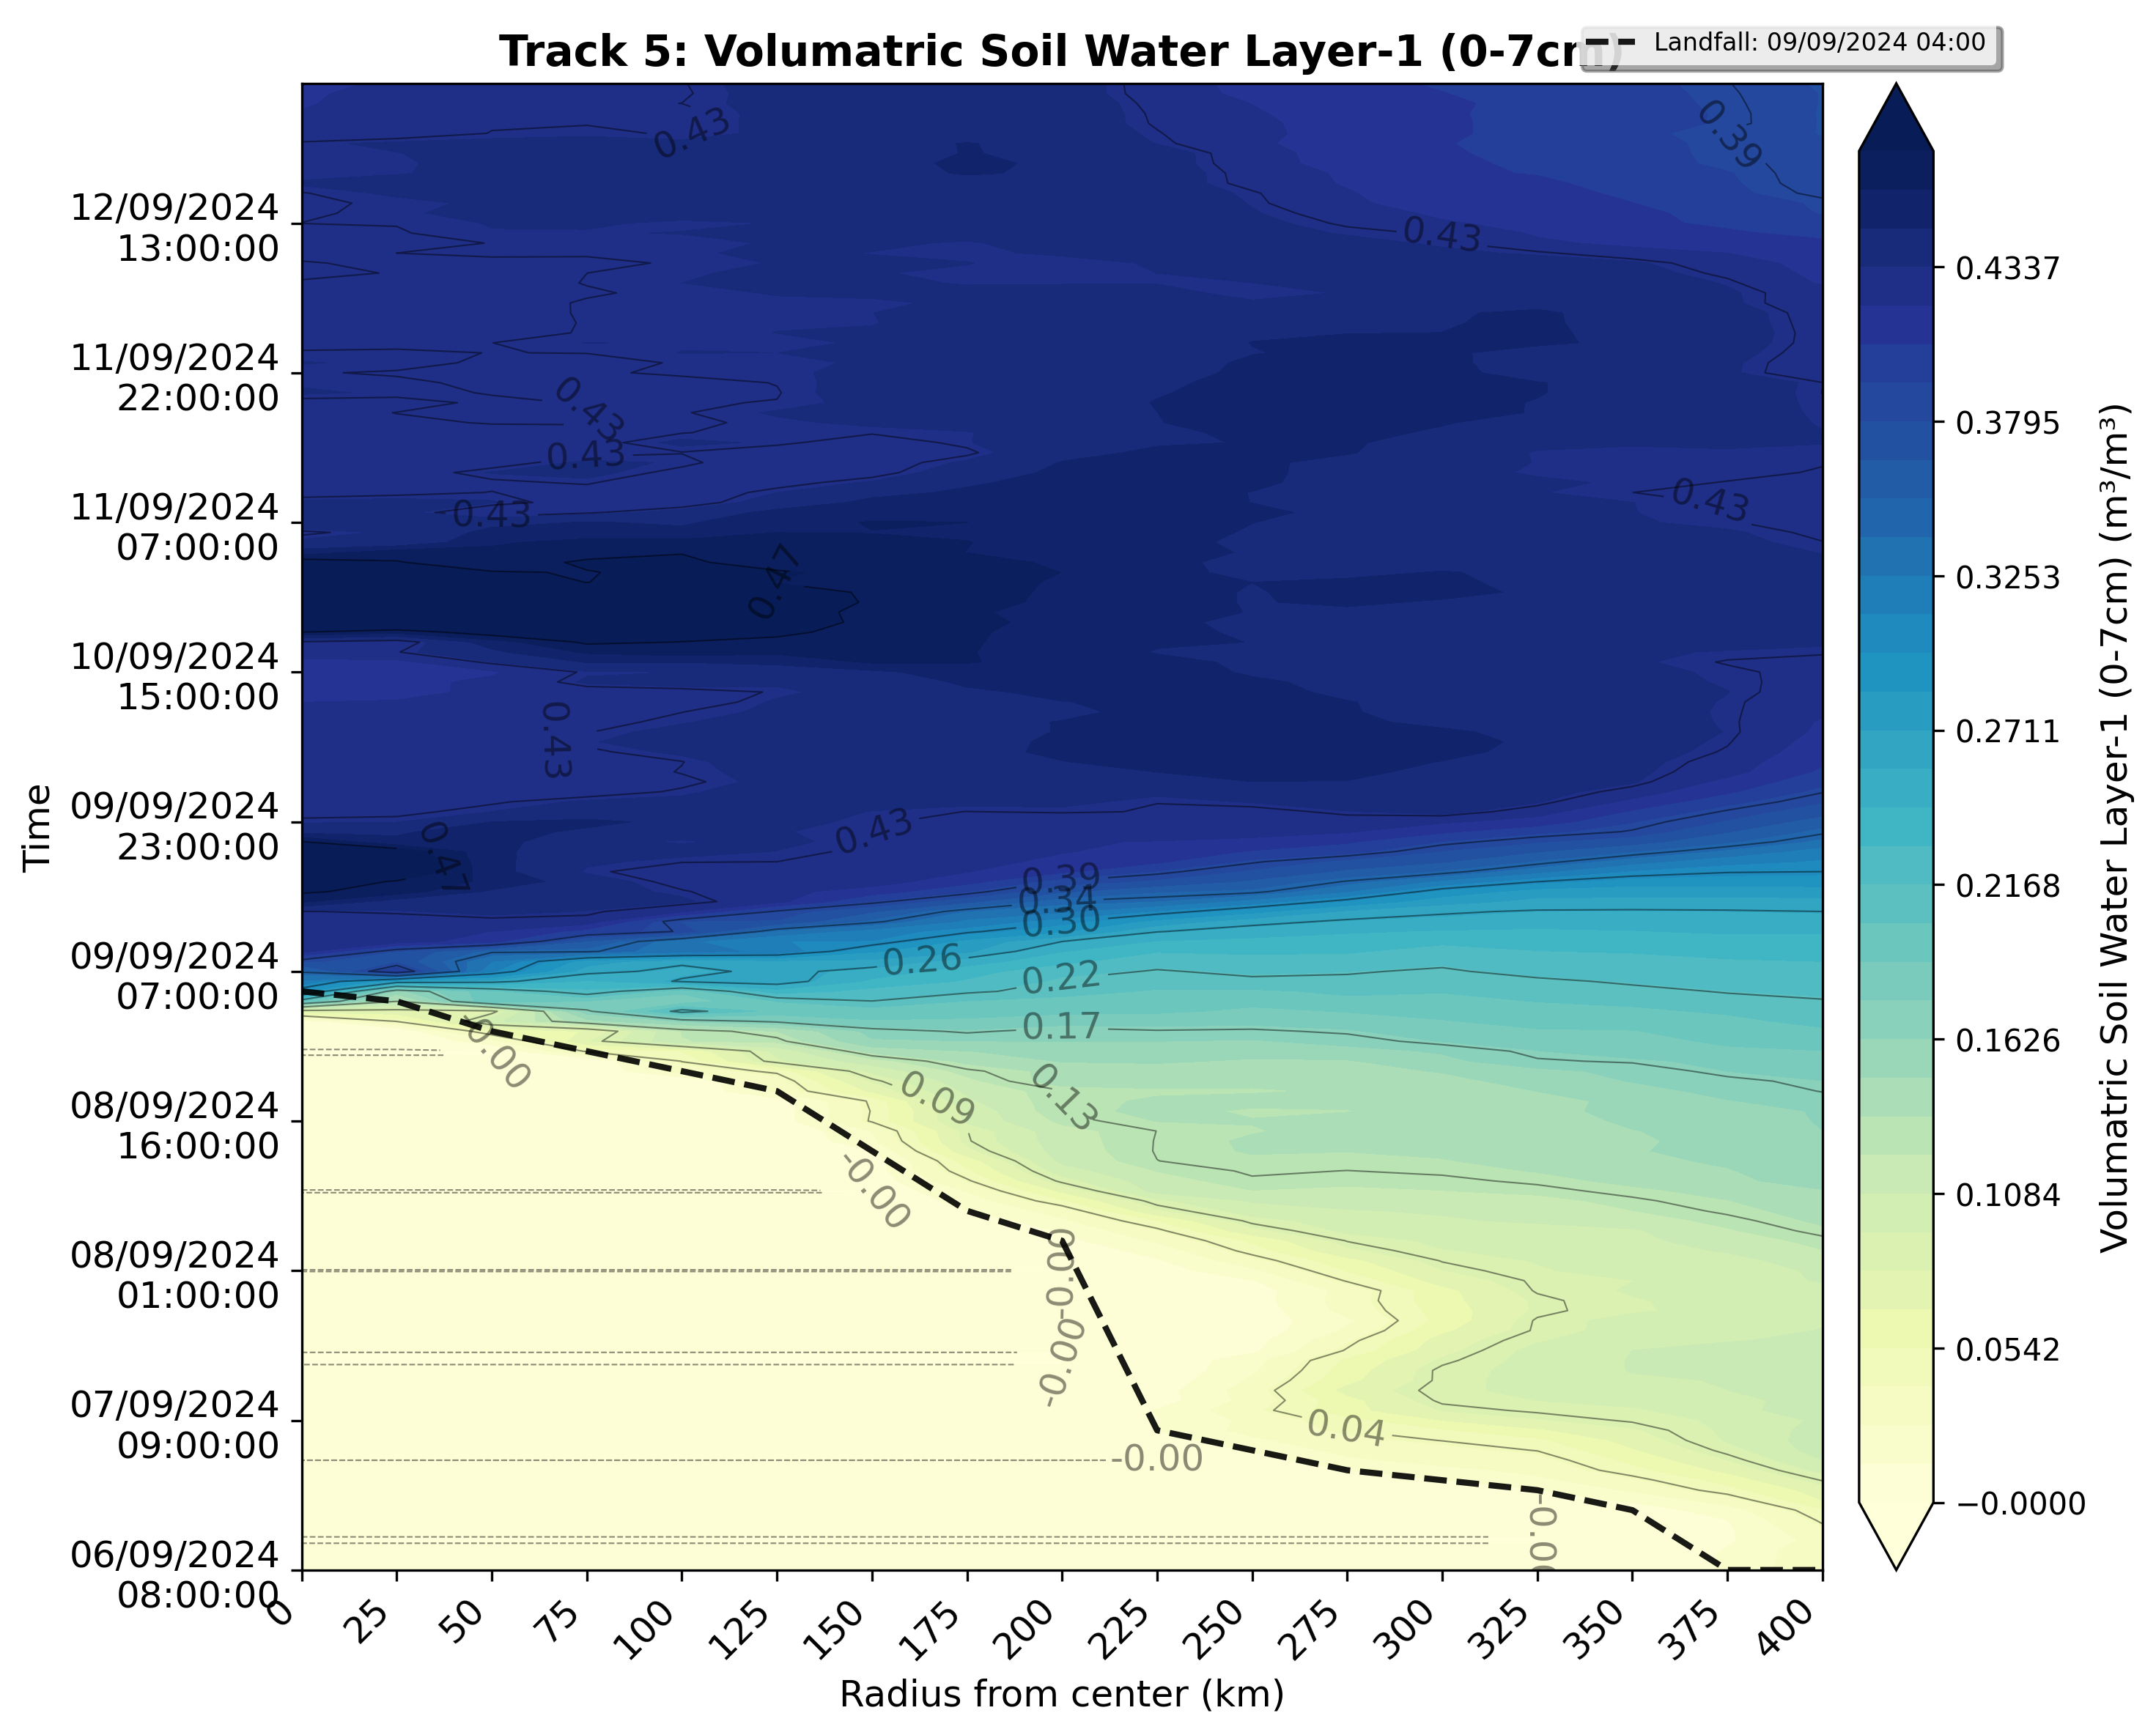
\includegraphics[width=0.69\textwidth]{track_long_swvl1_hov}
  \caption{BOE: Extended exposure to moist surface}
  \label{fig:hov_long_swvl1}
\end{figure}

\begin{figure}[H]
  \centering
  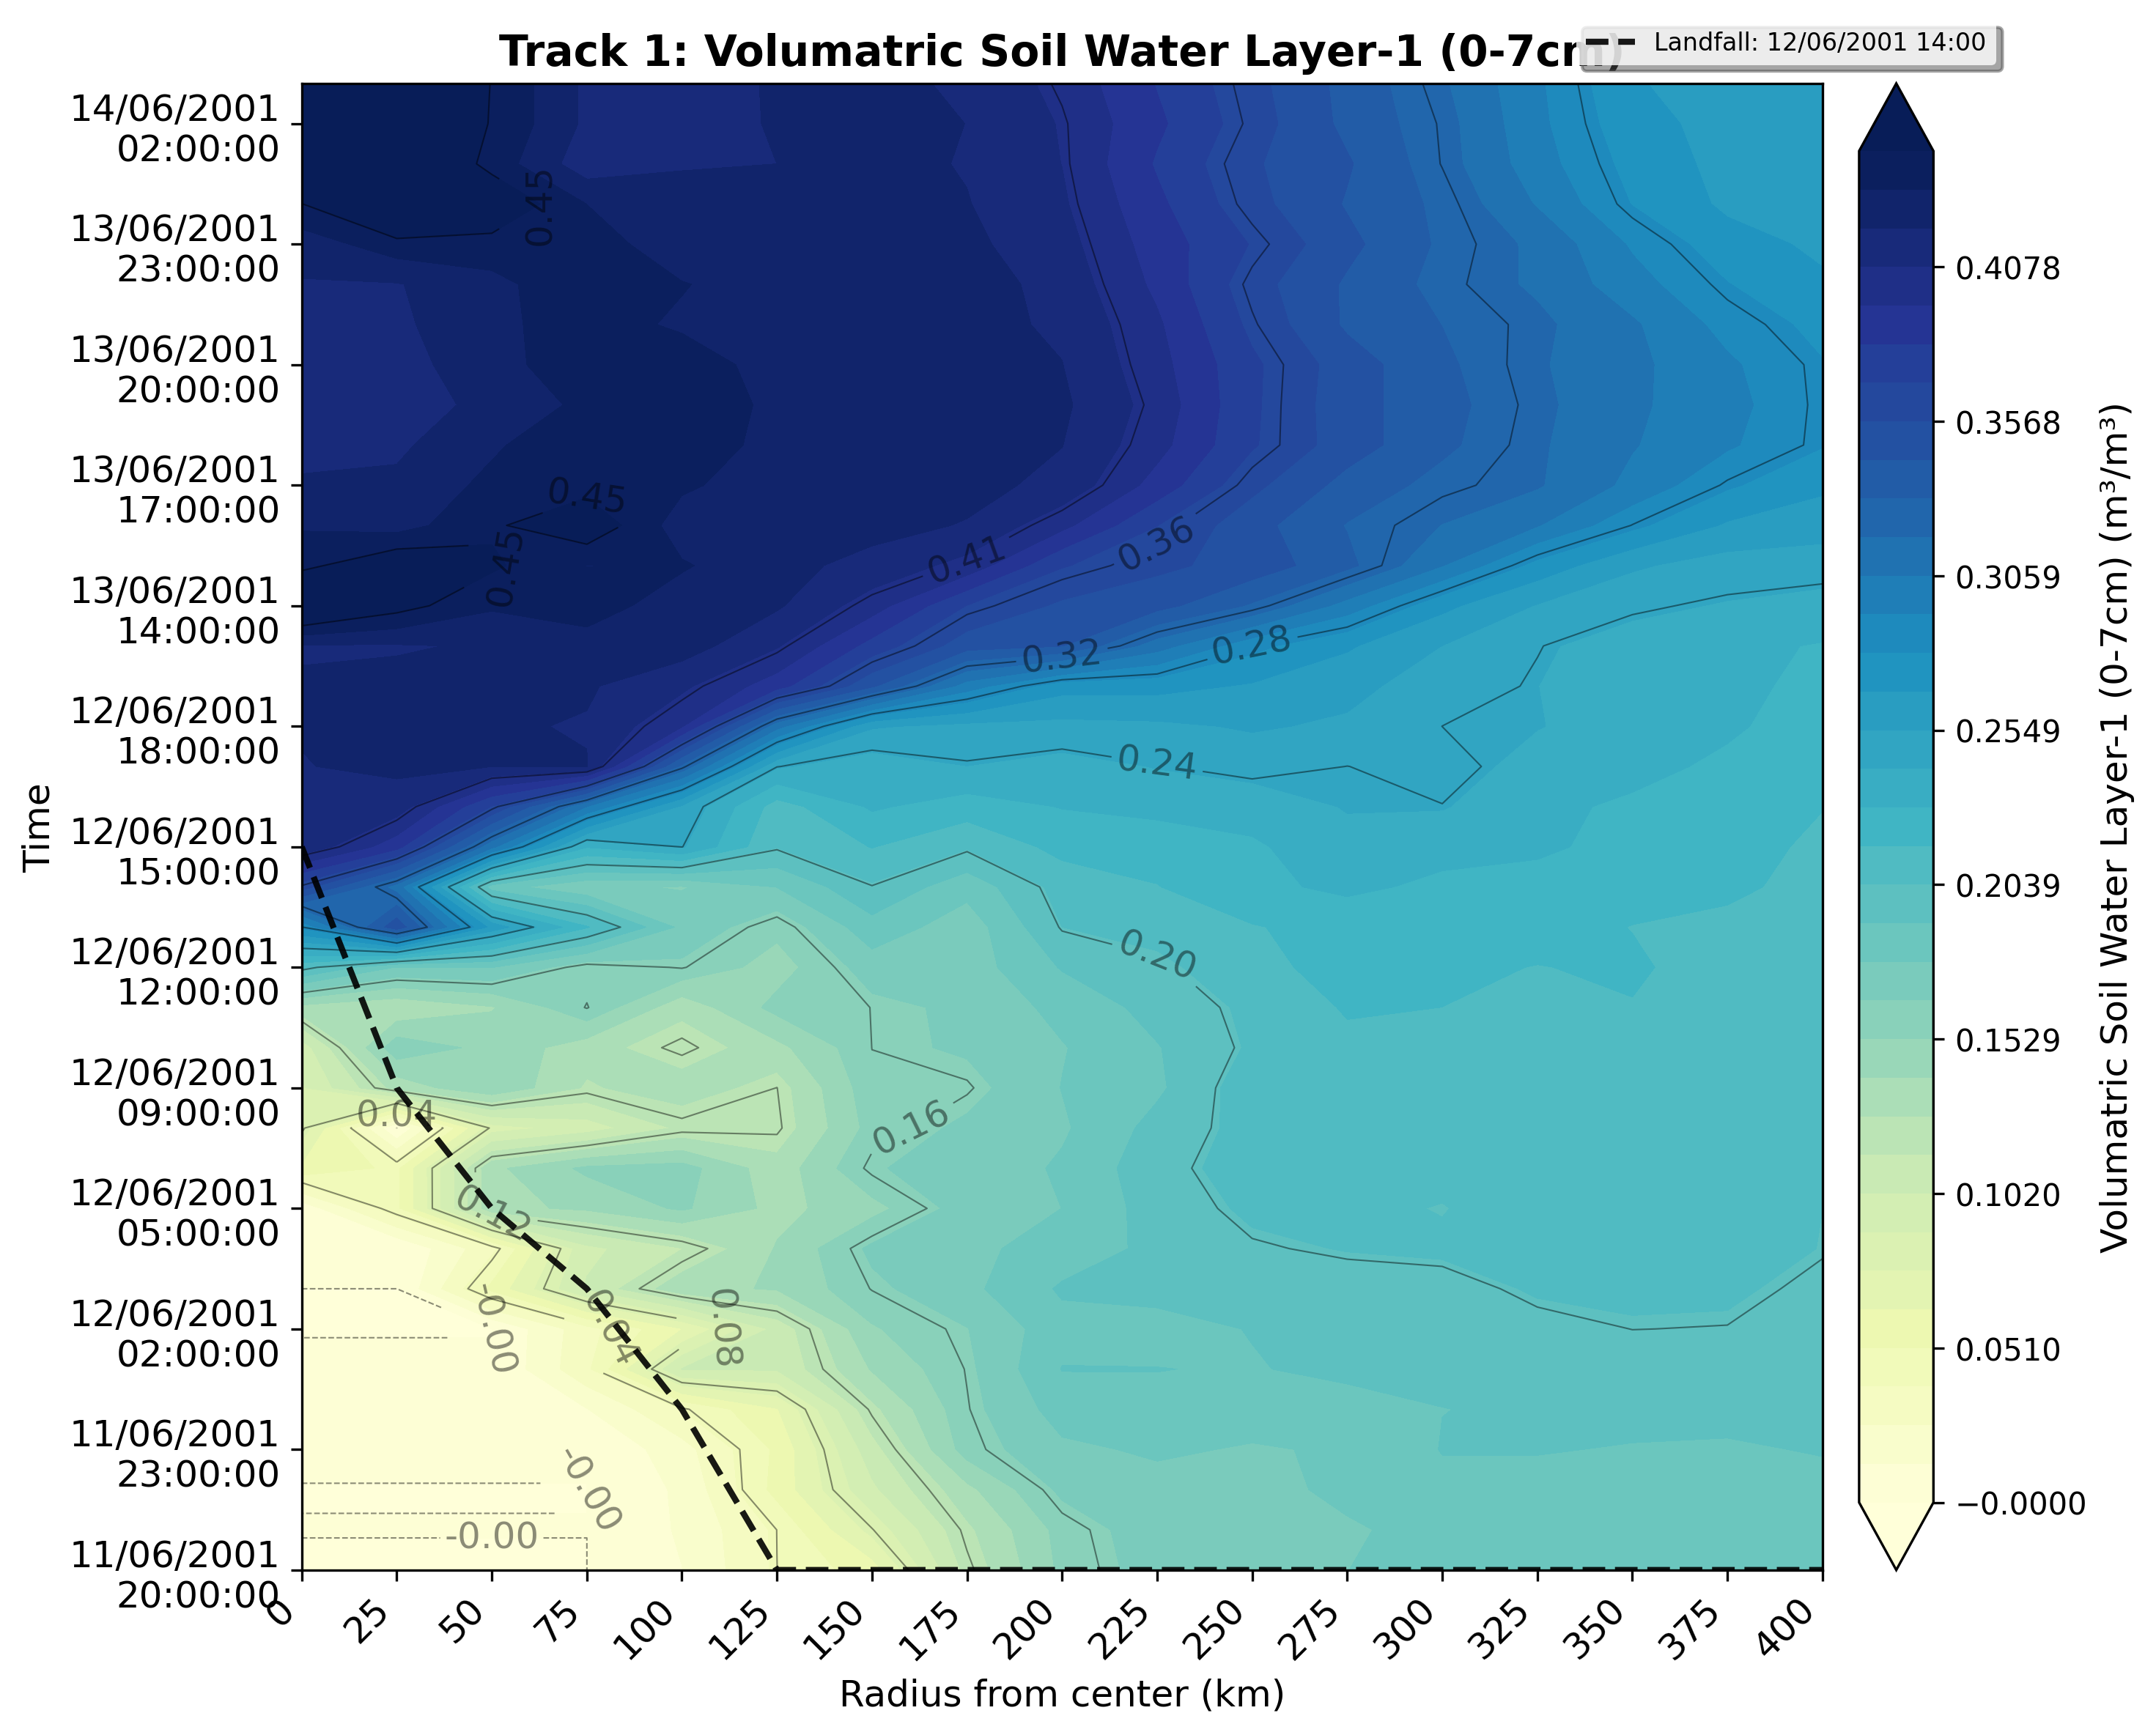
\includegraphics[width=0.69\textwidth]{track_short_swvl1_hov}
  \caption{Non-BOE: Rapid soil moisture decay}
  \label{fig:hov_short_swvl1}
\end{figure}

\subsection{Surface Latent Heat Flux: The BOE Energy Signal}
\label{subsec:hovmoller_slhtf}

The Surface Latent Heat Flux (\texttt{SLHTF}) provides the most direct measure
of the energy available to sustain the MD's secondary circulation. As
shown in Figure~\ref{fig:hov_long_slhtf} and \ref{fig:hov_short_slhtf}, both
long-lived and short-lived systems exhibit high oceanic LHF
magnitudes (ranging from $-220$ to $-150$\,W\,m$^{-2}$) prior to landfall.

The divergence in behavior occurs post-landfall ($t > 0$). In the
BOE-active case, the inner-core LHF stays effectively ``oceanic'' due
to the saturated soil state. This prevents the typical thermodynamic
decoupling that occurs when a storm moves over land. Conversely, in
non-BOE systems, the LHF is transient; the lack of a deep soil
moisture reservoir leads to a rapid collapse of the energy supply,
resulting in the dissipation of core convection.

\begin{figure}[H]
  \centering
  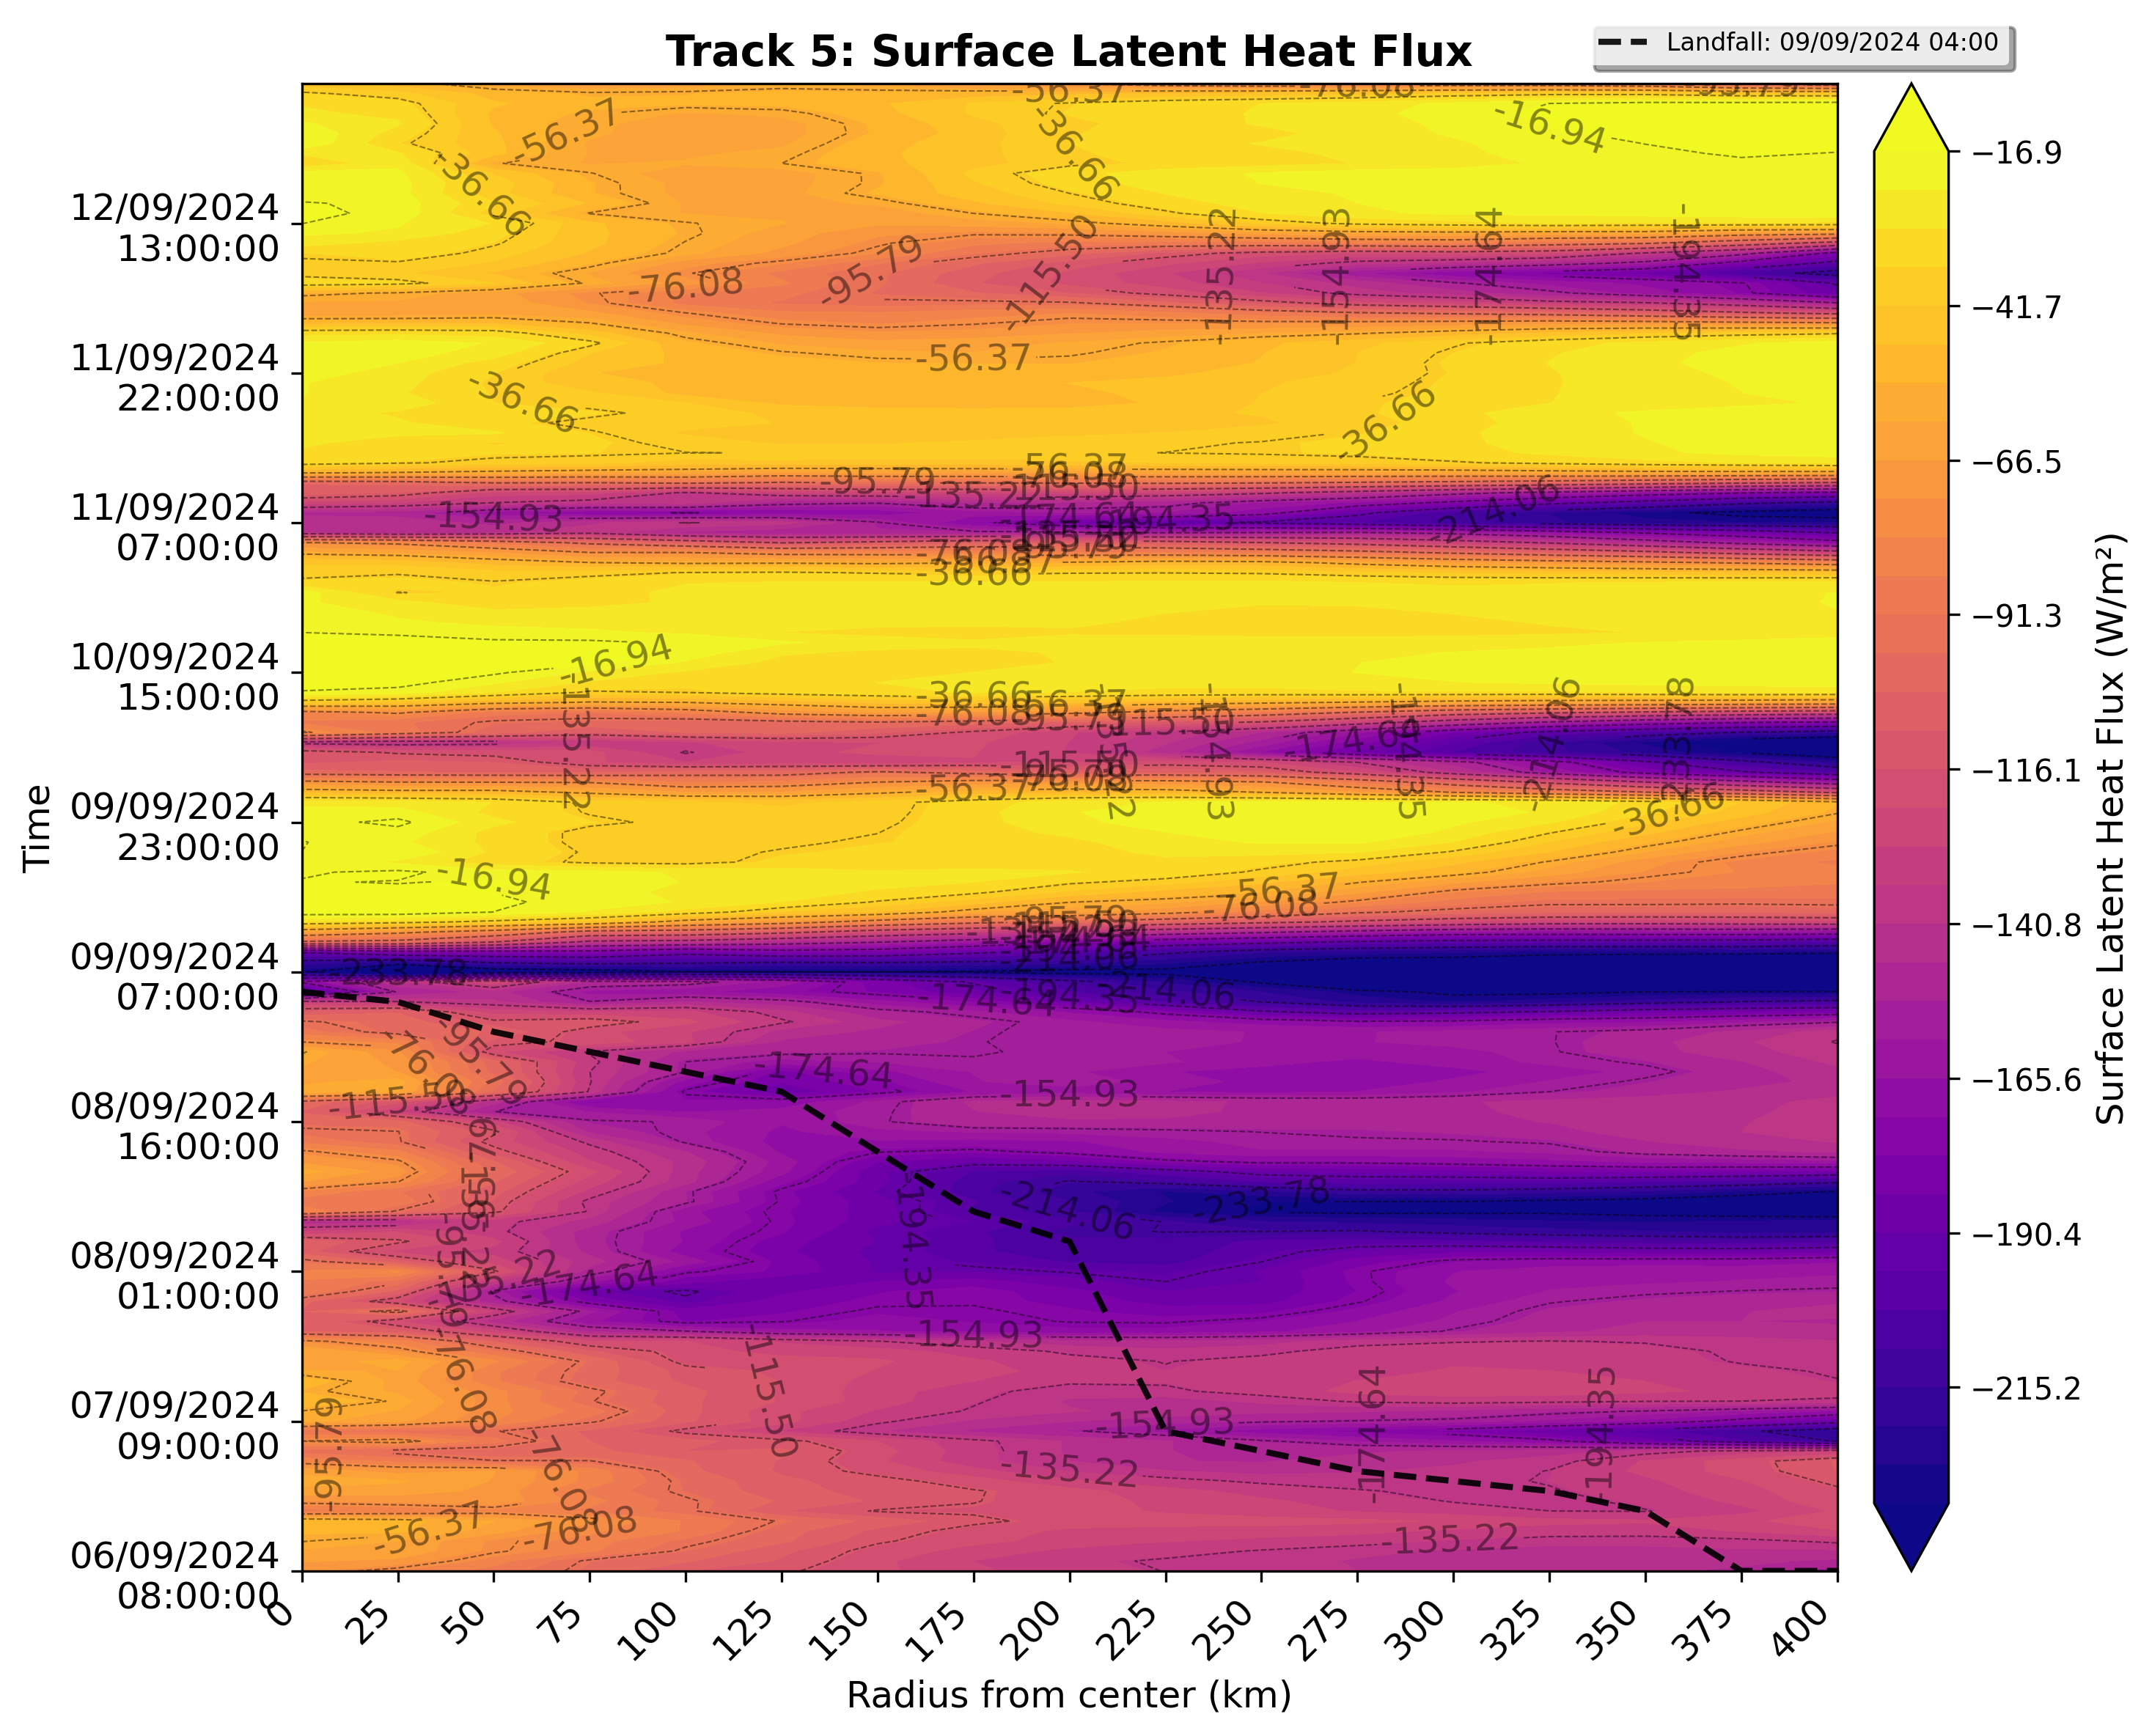
\includegraphics[width=0.69\textwidth]{track_long_slhtf_hov}
  \caption{BOE: Sustained land-phase flux}
  \label{fig:hov_long_slhtf}
\end{figure}

\begin{figure}[H]
  \centering
  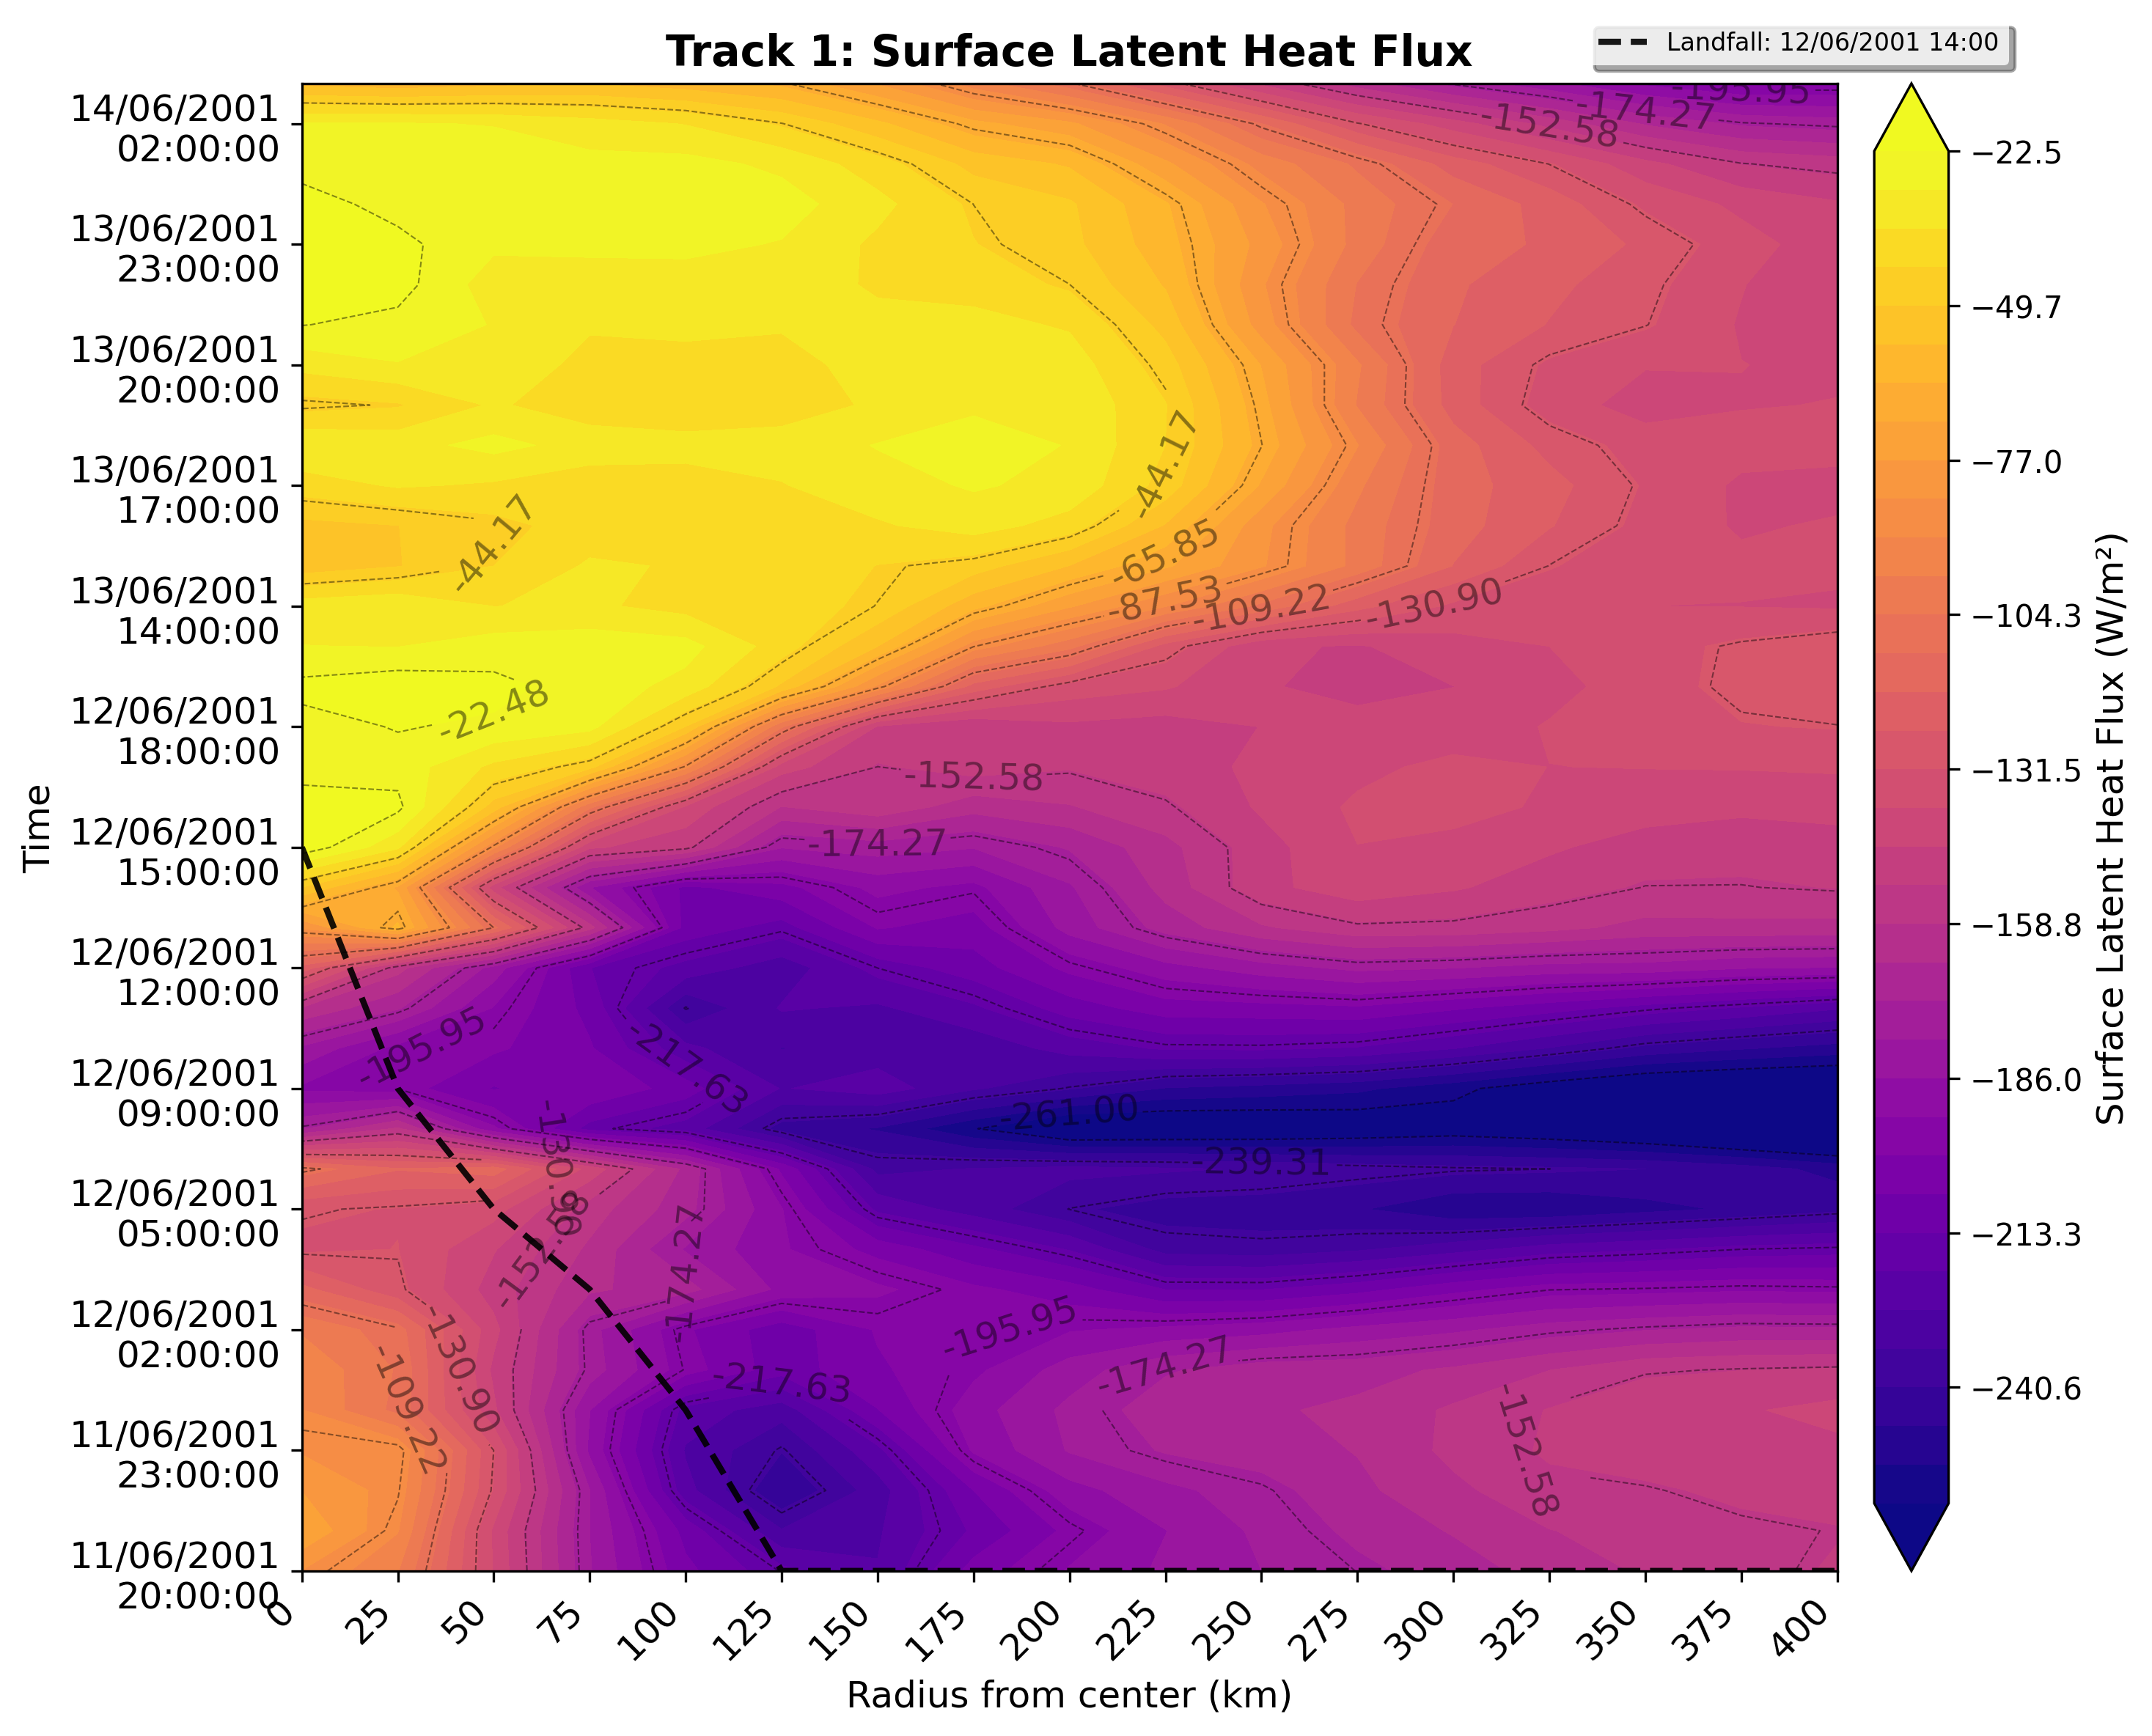
\includegraphics[width=0.69\textwidth]{track_short_slhtf_hov}
  \caption{Non-BOE: Transient flux collapse}
  \label{fig:hov_short_slhtf}
\end{figure}

Azimuthal Hovm\"{o}ller of Surface latent heat flux (\texttt{SLHTF})
(W\,m$^{-2}$), in the long-lived system
(Figure~\ref{fig:hov_long_slhtf}), LHF remains consistently above the
sustaining threshold ($>70$\,W\,m$^{-2}$) for over 48 hours inland.
While in the short-lived system (Figure~\ref{fig:hov_short_slhtf}),
the flux collapses within 12-18 hours of landfall despite similar
initial ranges.

\subsection{Surface Sensible Heat Flux: Thermal Feedback}
\label{subsec:hovmoller_ishf}

The Surface Sensible Heat Flux (\texttt{ISHF}) diagnostics
(Figure~\ref{fig:hov_long_ishf} and \ref{fig:hov_short_ishf}) reveal
the thermal state of the boundary layer. Over the ocean, both systems
maintain near-neutral SHF values ($-12$ to $-17$\,W\,m$^{-2}$),
indicating thermal equilibrium with the Bay of Bengal.

\begin{figure}[H]
  \centering
  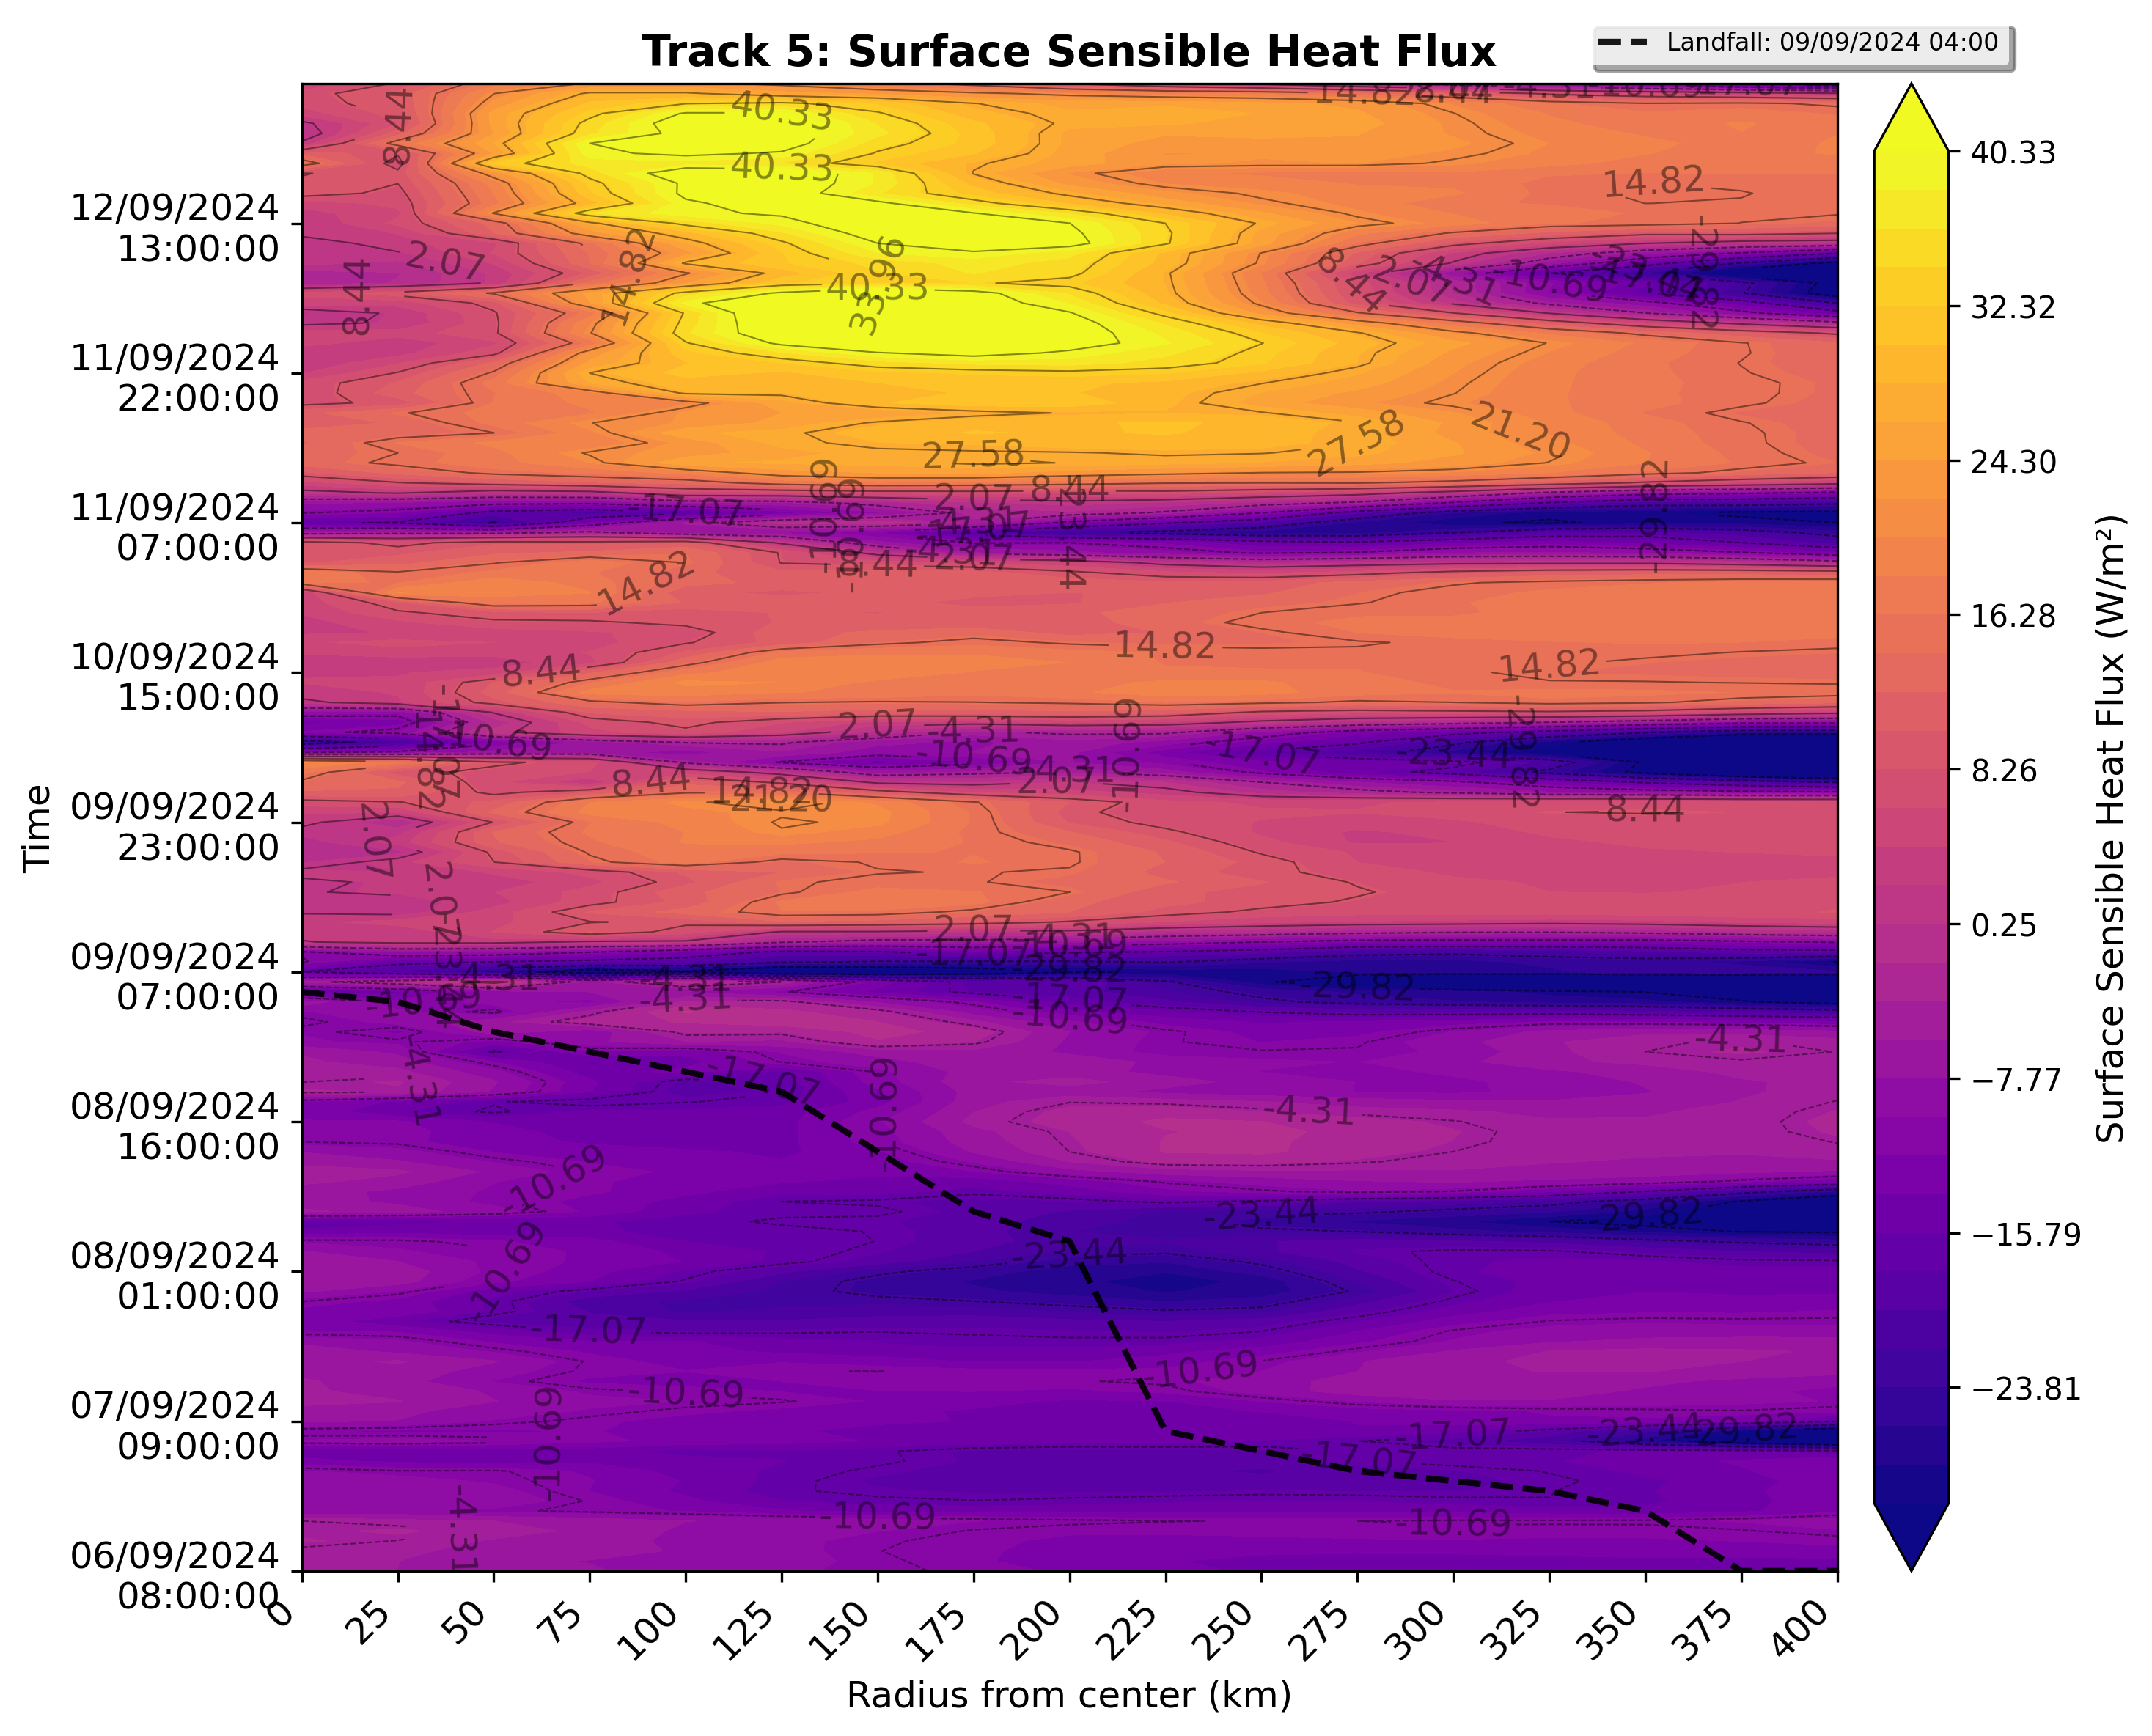
\includegraphics[width=0.67\textwidth]{track_long_ishf_hov}
  \caption{BOE: Suppressed sensible heating}
  \label{fig:hov_long_ishf}
\end{figure}

\begin{figure}[H]
  \centering
  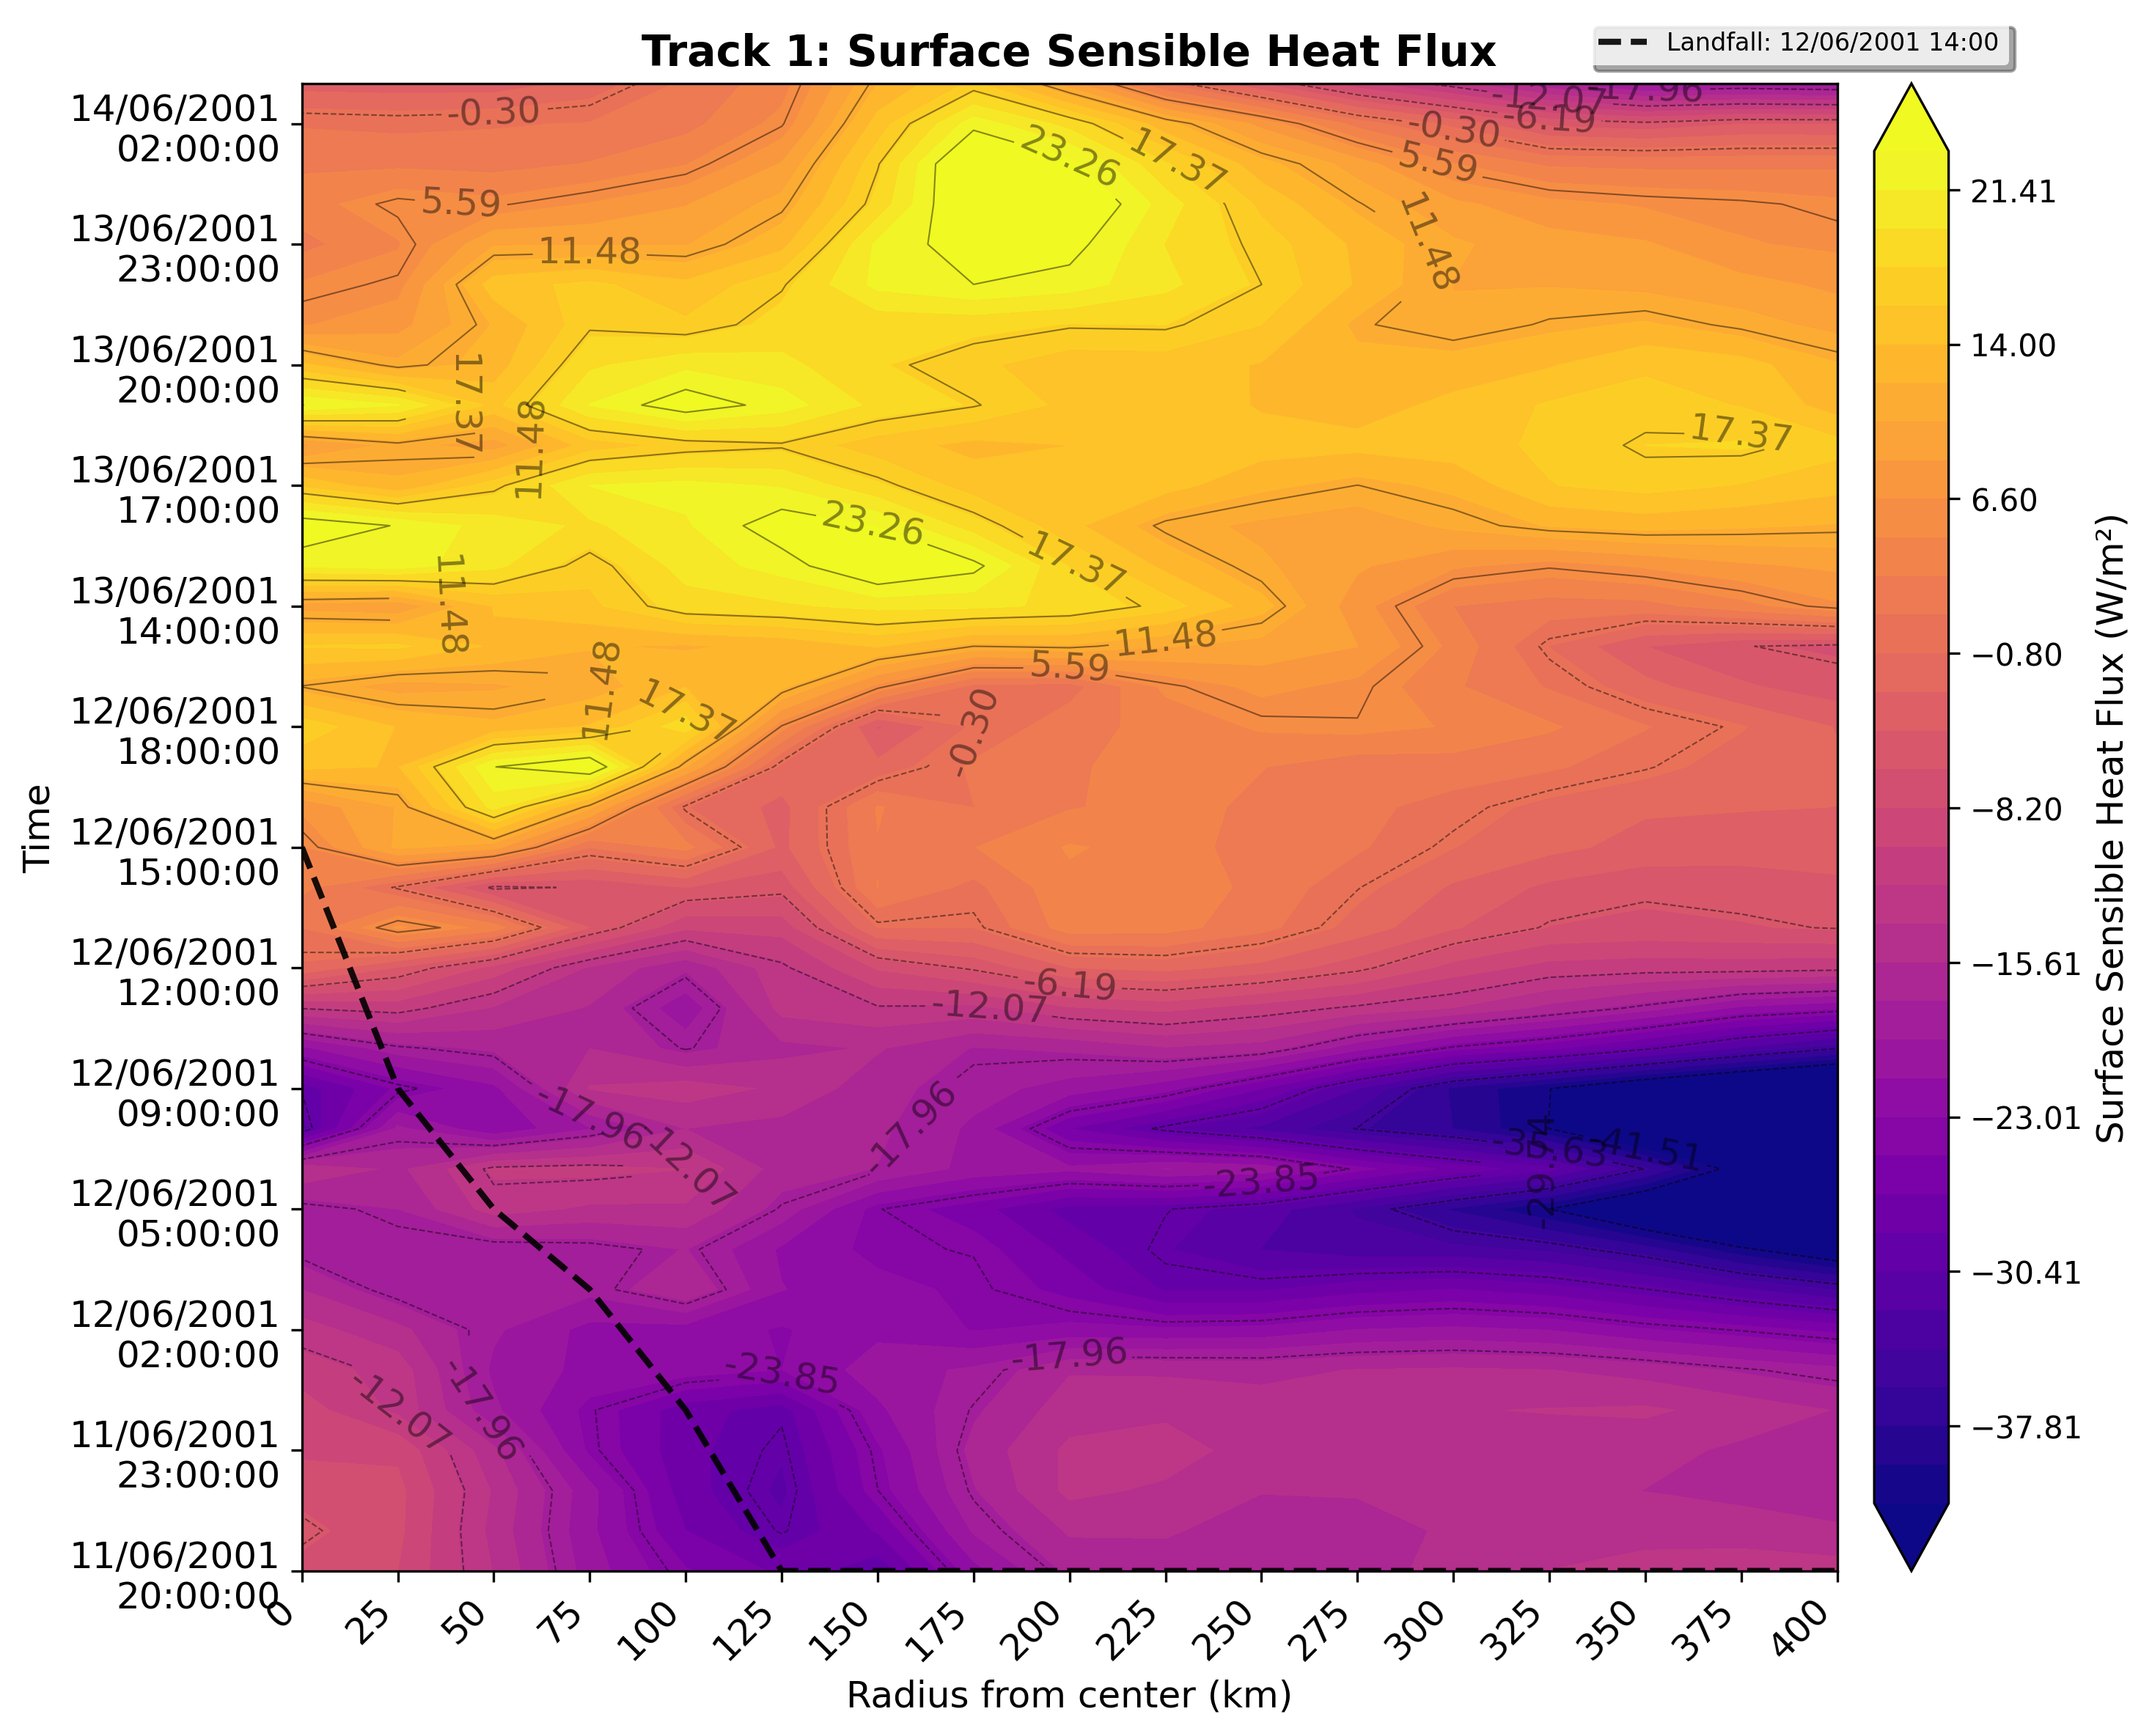
\includegraphics[width=0.67\textwidth]{track_short_ishf_hov}
  \caption{Non-BOE: Thermal destabilization}
  \label{fig:hov_short_ishf}
\end{figure}

Upon landfall, the BOE-active system (Figure~\ref{fig:hov_long_ishf})
maintains low Sensible heat flux on land; the energy is partitioned
into latent rather than sensible heat, keeping the inner core cool
and saturated, which is essential for vortex maintenance. In
contrast, the short-lived system encounters a stable thermal
environment, with SHF reaching extremes of 21\,W\,m$^{-2}$ (downward)
to $-37$\,W\,m$^{-2}$ (upward). This rapid sensible heating from a
dry surface increases the boundary layer height and encourages
dry-air entrainment.

Azimuthal Hovm\"{o}ller of SSHF (W\,m$^{-2}$). The non-BOE system
(Figure~\ref{fig:hov_short_ishf}) shows extreme fluctuations at
landfall (ranging from 21 to $-37$\,W\,m$^{-2}$), indicating a hot,
dry surface that disrupts the saturated inner-core structure after
encountering landfall.

\subsection{Dew Point Temperature: Boundary Layer Saturation and Maintenance}
\label{subsec:hovmoller_d2m}

% The 2-m dew point temperature ($d2m$) Hovm\"{o}ller results
% (Figure~\ref{fig:hov_track_comparison_d2m}) serve as a diagnostic for
% the moisture state of the boundary layer, complementing the energy
% flux analysis in Section~\ref{subsec:hovmoller_slhtf}. While both
% long-lived and short-lived systems eventually reach a minimum dew
% point of $\sim$295\,K, the \textbf{timescale of desipation} varies
% significantly, marking the difference between a system that carries
% its environment inland and one that succumb to continental drying.

The azimuthal hovm\"{o}ller evolution of 2-m dew point temperature
(\texttt{D2M}) illustrates how BOE-active systems maintain a
maritime-like boundary layer deep into the inland. While both
eventually settle toward a floor value of $\sim$295--296\,K, the
distinction lies in the \textbf{moisture decay rate} following landfall
(Figure~\ref{fig:hov_long_d2m} and \ref{fig:hov_short_d2m}).

\begin{figure}[H]
  \centering
  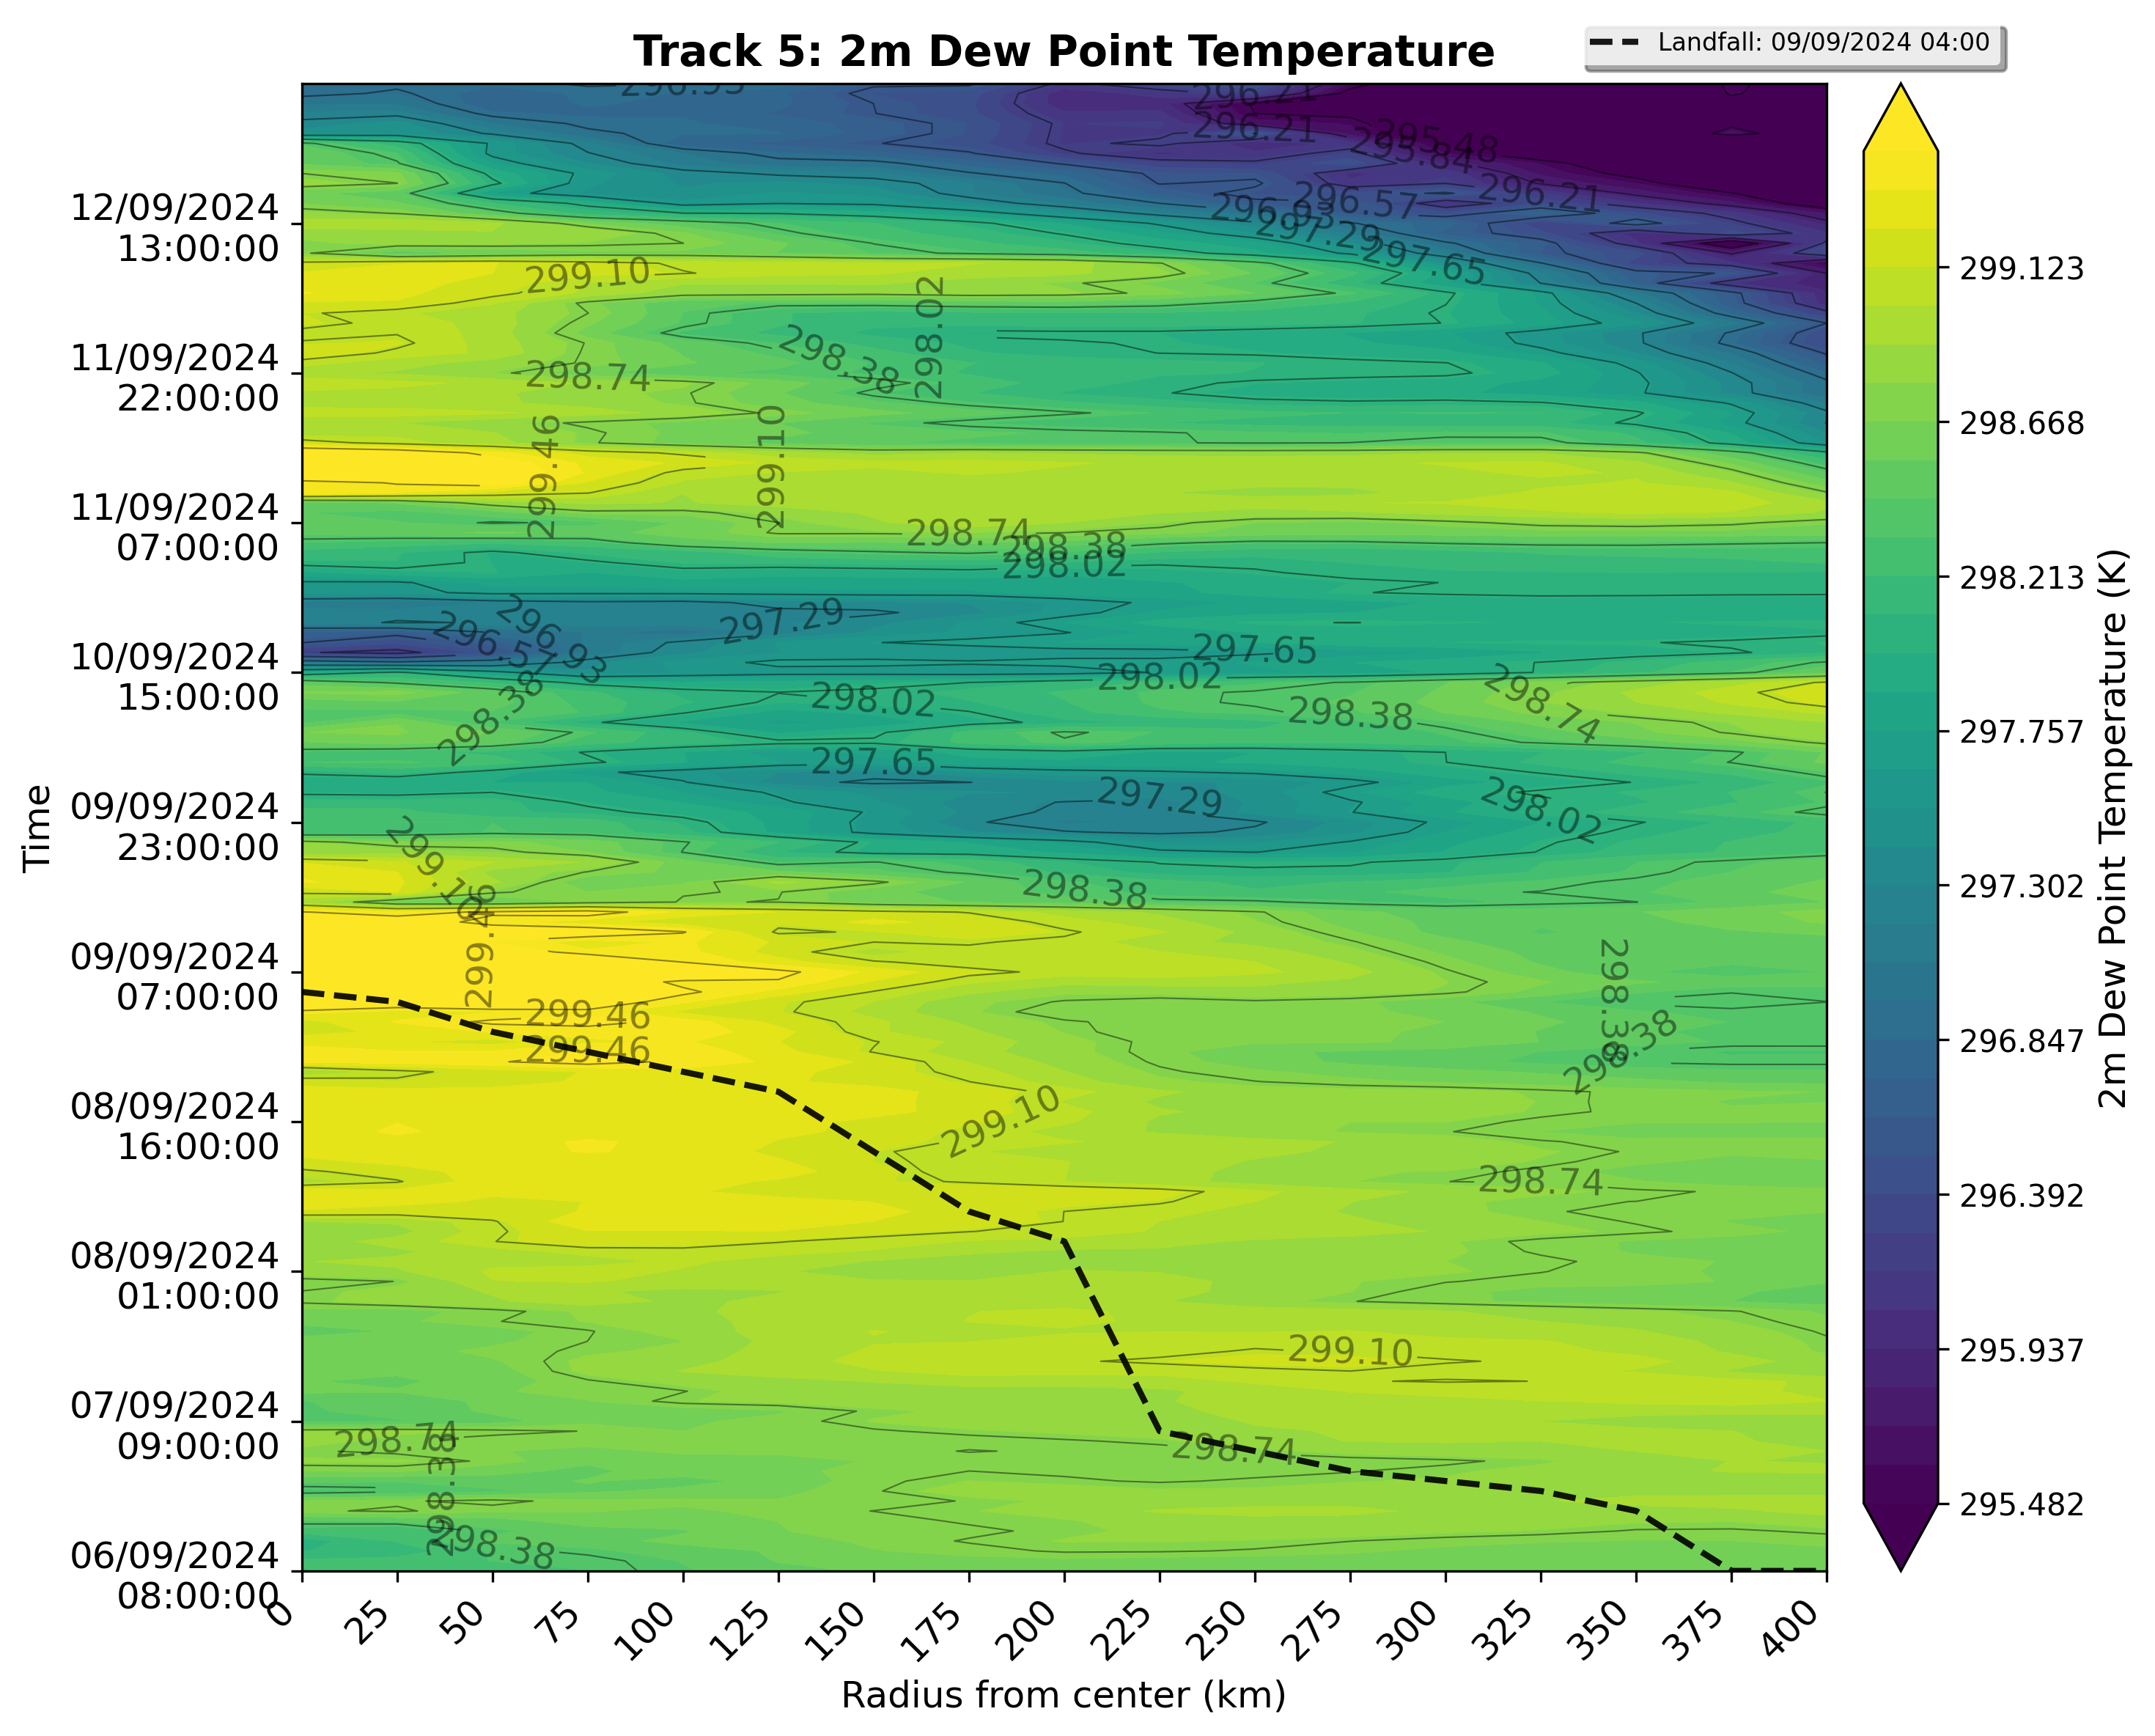
\includegraphics[width=0.69\textwidth]{track_long_d2m_hov}
  \caption{BOE: Sustained moisture saturation}
  \label{fig:hov_long_d2m}
\end{figure}

\begin{figure}[H]
  \centering
  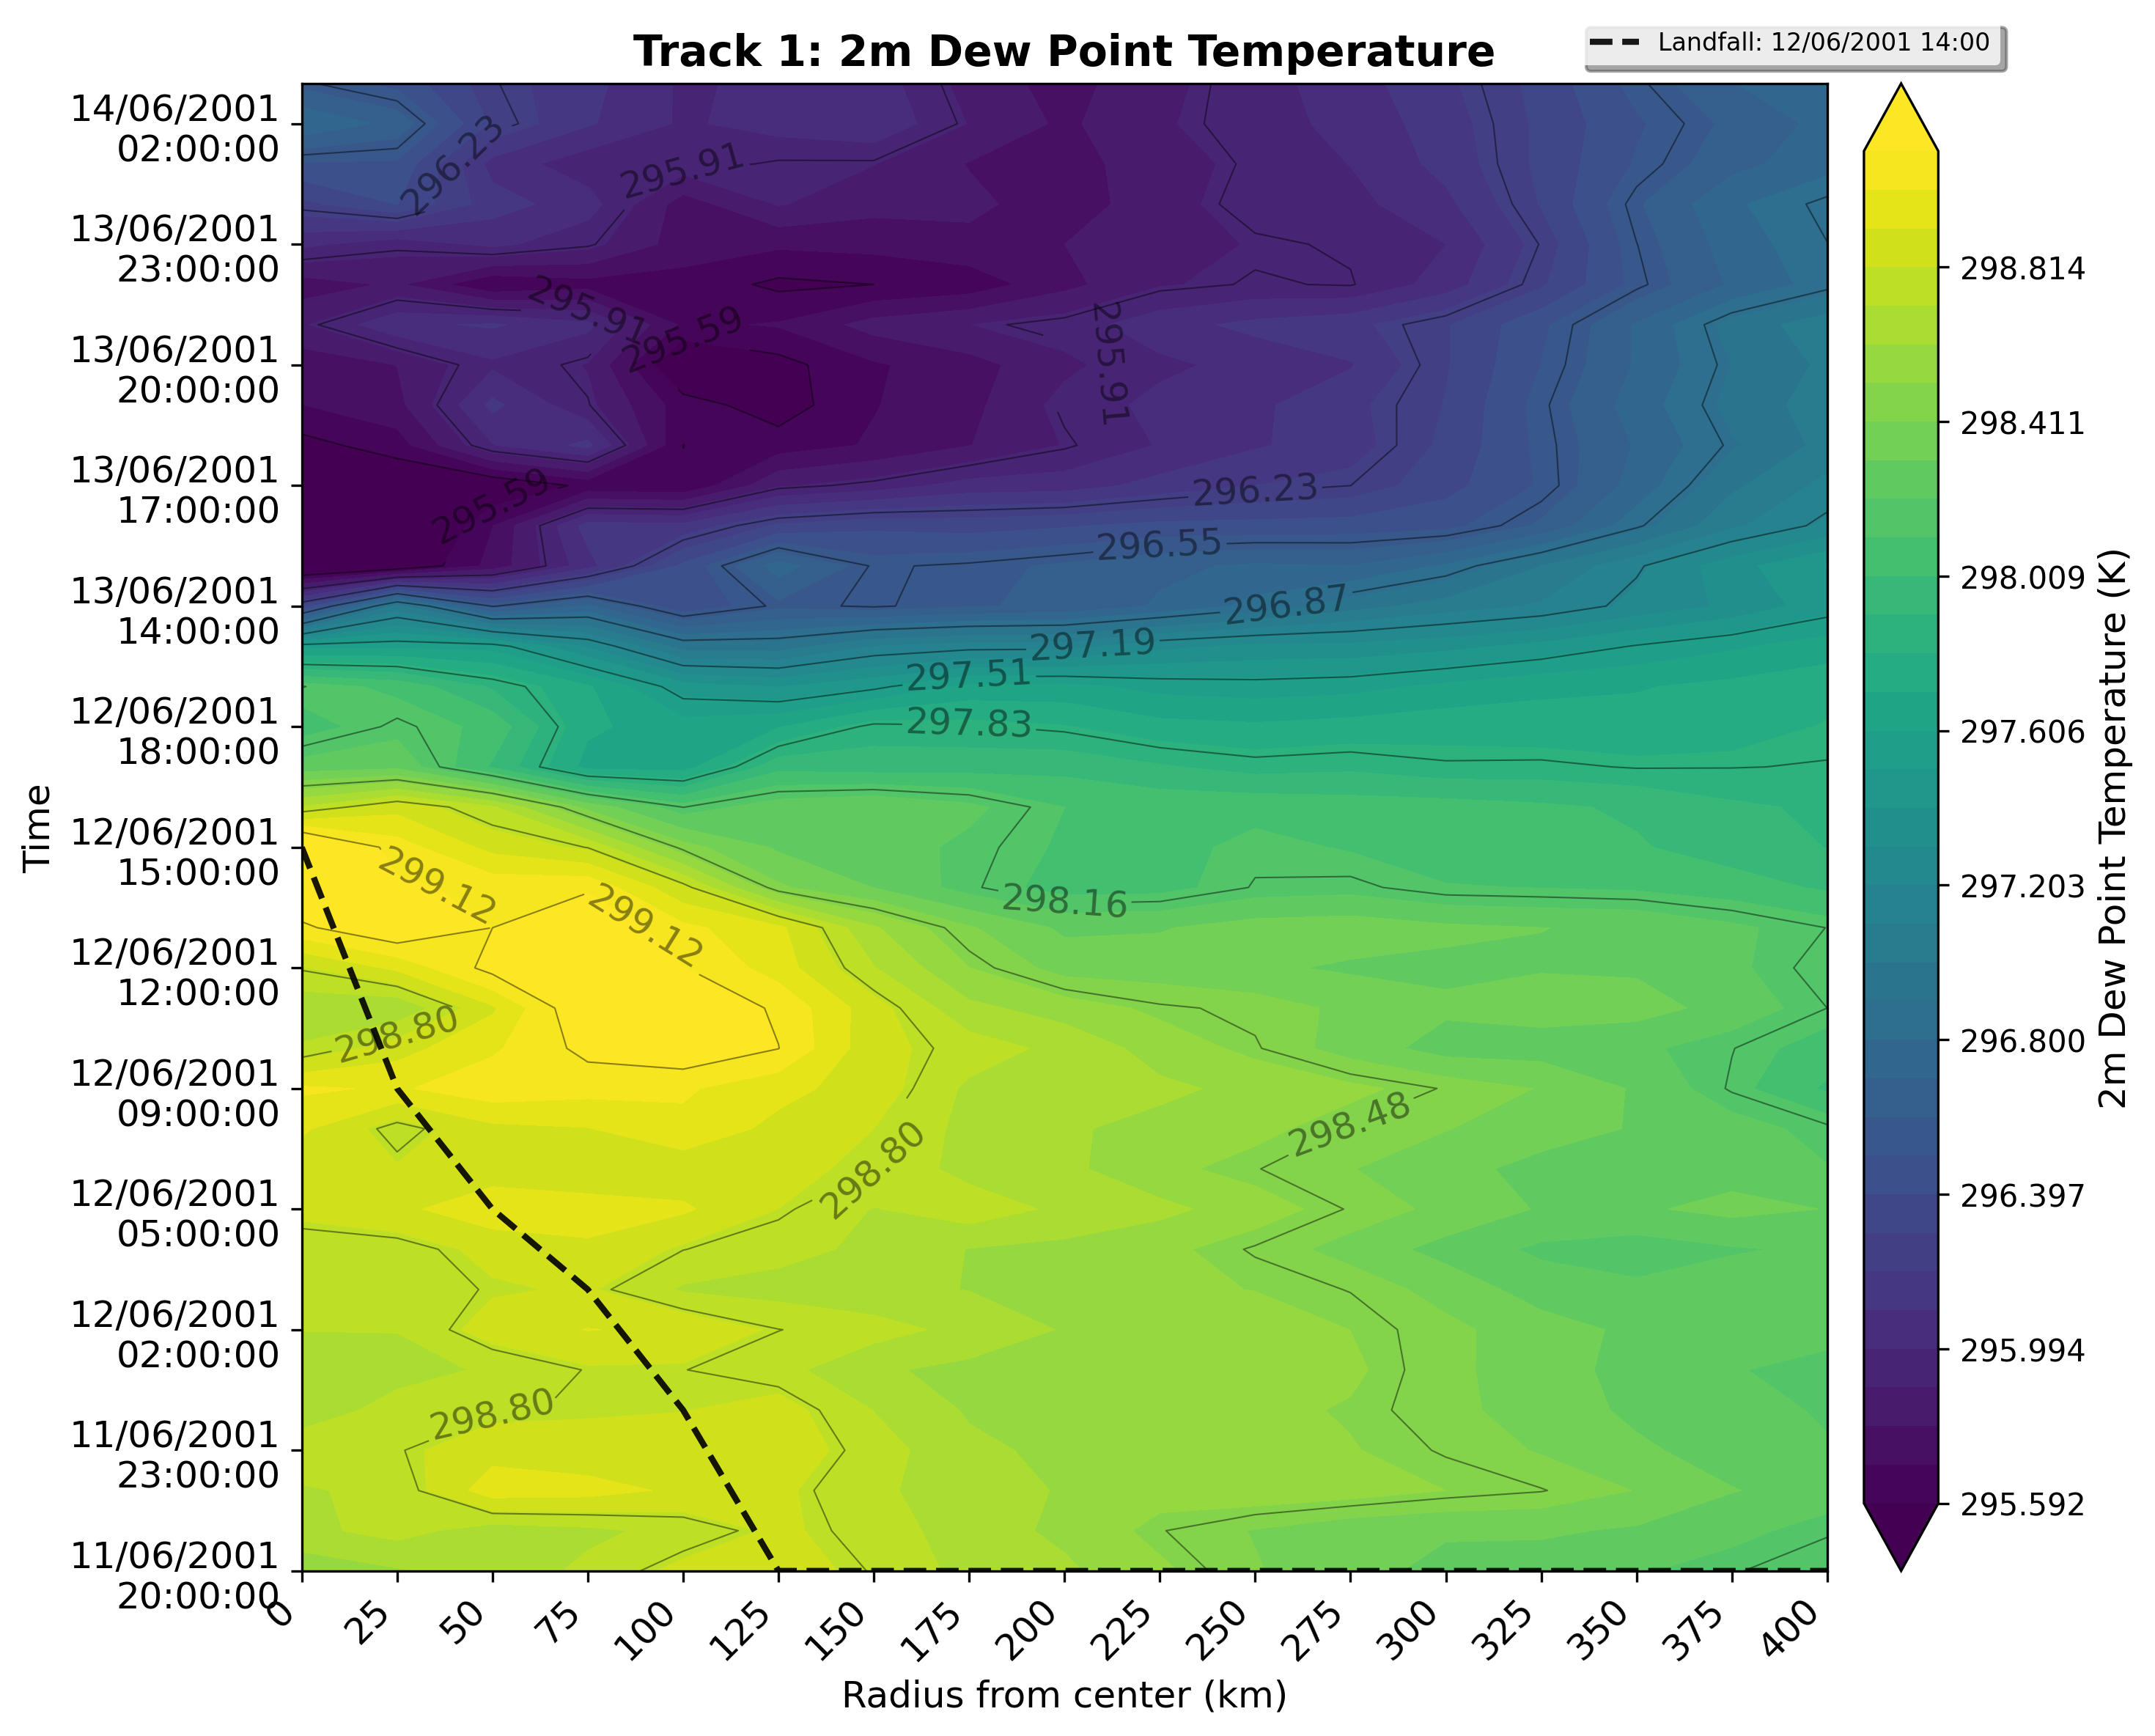
\includegraphics[width=0.69\textwidth]{track_short_d2m_hov}
  \caption{Non-BOE: Rapid boundary layer drying}
  \label{fig:hov_short_d2m}
\end{figure}

Azimuthal Hovm\"{o}ller of 2-m dew point temperature (\texttt{D2M}).
The long-lived system (Figure~\ref{fig:hov_long_d2m}) maintains a
high moisture floor ($>298$\,K) for over 72 hours, whereas the
short-lived system (Figure~\ref{fig:hov_short_d2m}) drops to values
almost immediately after landfall.

In a standard landfall scenario, the removal of the maritime moisture
source should trigger a rapid drop in \texttt{D2M}. This is observed in the
short-lived population (Figure~\ref{fig:hov_short_d2m}), where
\texttt{D2M} falls toward 296\,K within 12-24 hours. This drop increases
the Dew Point Depression (DPD), raising the Lifting Condensation
Level (LCL) and effectively dissipating the core convection.

However, long-lived MDs exhibit a moisture maintenance signal. By
sustaining \texttt{D2M} at 298--299\,K deep into the land phase and for
longer time period, these systems effectively carry their own
environment inland. This maintenance is a direct physical consequence
of the soil moisture and LHF feedbacks described in previous sections:
\begin{itemize}
  \item \textbf{Recycling:} The wet soil reservoir identified in
    Section~\ref{subsec:hovmoller_swvl1} evaporates moisture back
    into the boundary layer via sustained LHF
    (Section~\ref{subsec:hovmoller_slhtf}).
  \item \textbf{Low-Altitude Latent Heat:} Keeping the boundary layer
    near saturation (high \texttt{D2M}) ensures a very low LCL. This allows
    latent heat to be released at lower altitudes, keeping the vortex
    structurally strong and resisting the shear that typically
    dissipates land-falling systems.
\end{itemize}

Ultimately, the transition from 299\,K to 296\,K represents the shift
from a saturated, ``ocean-like'' boundary layer to an unsaturated
continental one. The BOE-active systems delay this transition
indefinitely through local moisture recycling, providing the
thermodynamic fuel necessary for their longer inland penetration.

\section{The Elevation Barrier vs. Thermodynamic Escape}
\label{sec:results_elevation}

The transition of a Monsoon Depression (MD) from the Bay of Bengal to
the Indian landmass is characterized by a competition between
mechanical dissipation and thermodynamic maintenance. The 600,m
contour of the Eastern Ghats serves as a critical spatial gatekeeper
in this process.

As shown in Figures~\ref{fig:long_elevated} and
\ref{fig:short_elevated}, short-lived systems typically terminate
within 100,km of the coastline. For these systems, the increase in
surface roughness and the energy cost of orographic lifting consume
the system's remaining oceanic kinetic energy. Without a terrestrial
energy source to offset these losses, the vortex structure undergoes
rapid frictional collapse.

Conversely, long-lived tracks exhibit what can be termed a
\textbf{Thermodynamic Escape}. While these systems experience the
same initial mechanical deceleration upon encountering the terrain,
the orographic ascent triggers a concentrated burst of precipitation.
As detailed in Section~\ref{subsec:hovmoller_tp}, this rainfall
initiates the self-wetting feedback loop. Only systems that possess
the synchronized BOE signature-specifically high \texttt{LHF},
sustained \texttt{D2M}, and a contracted \texttt{TP} core-have the
energetic resilience to overcome the frictional penalty of the
terrain and reorganize on the leeward side of the Ghats.

\vfill

\newpage

\begin{figure}[H]
  \centering
  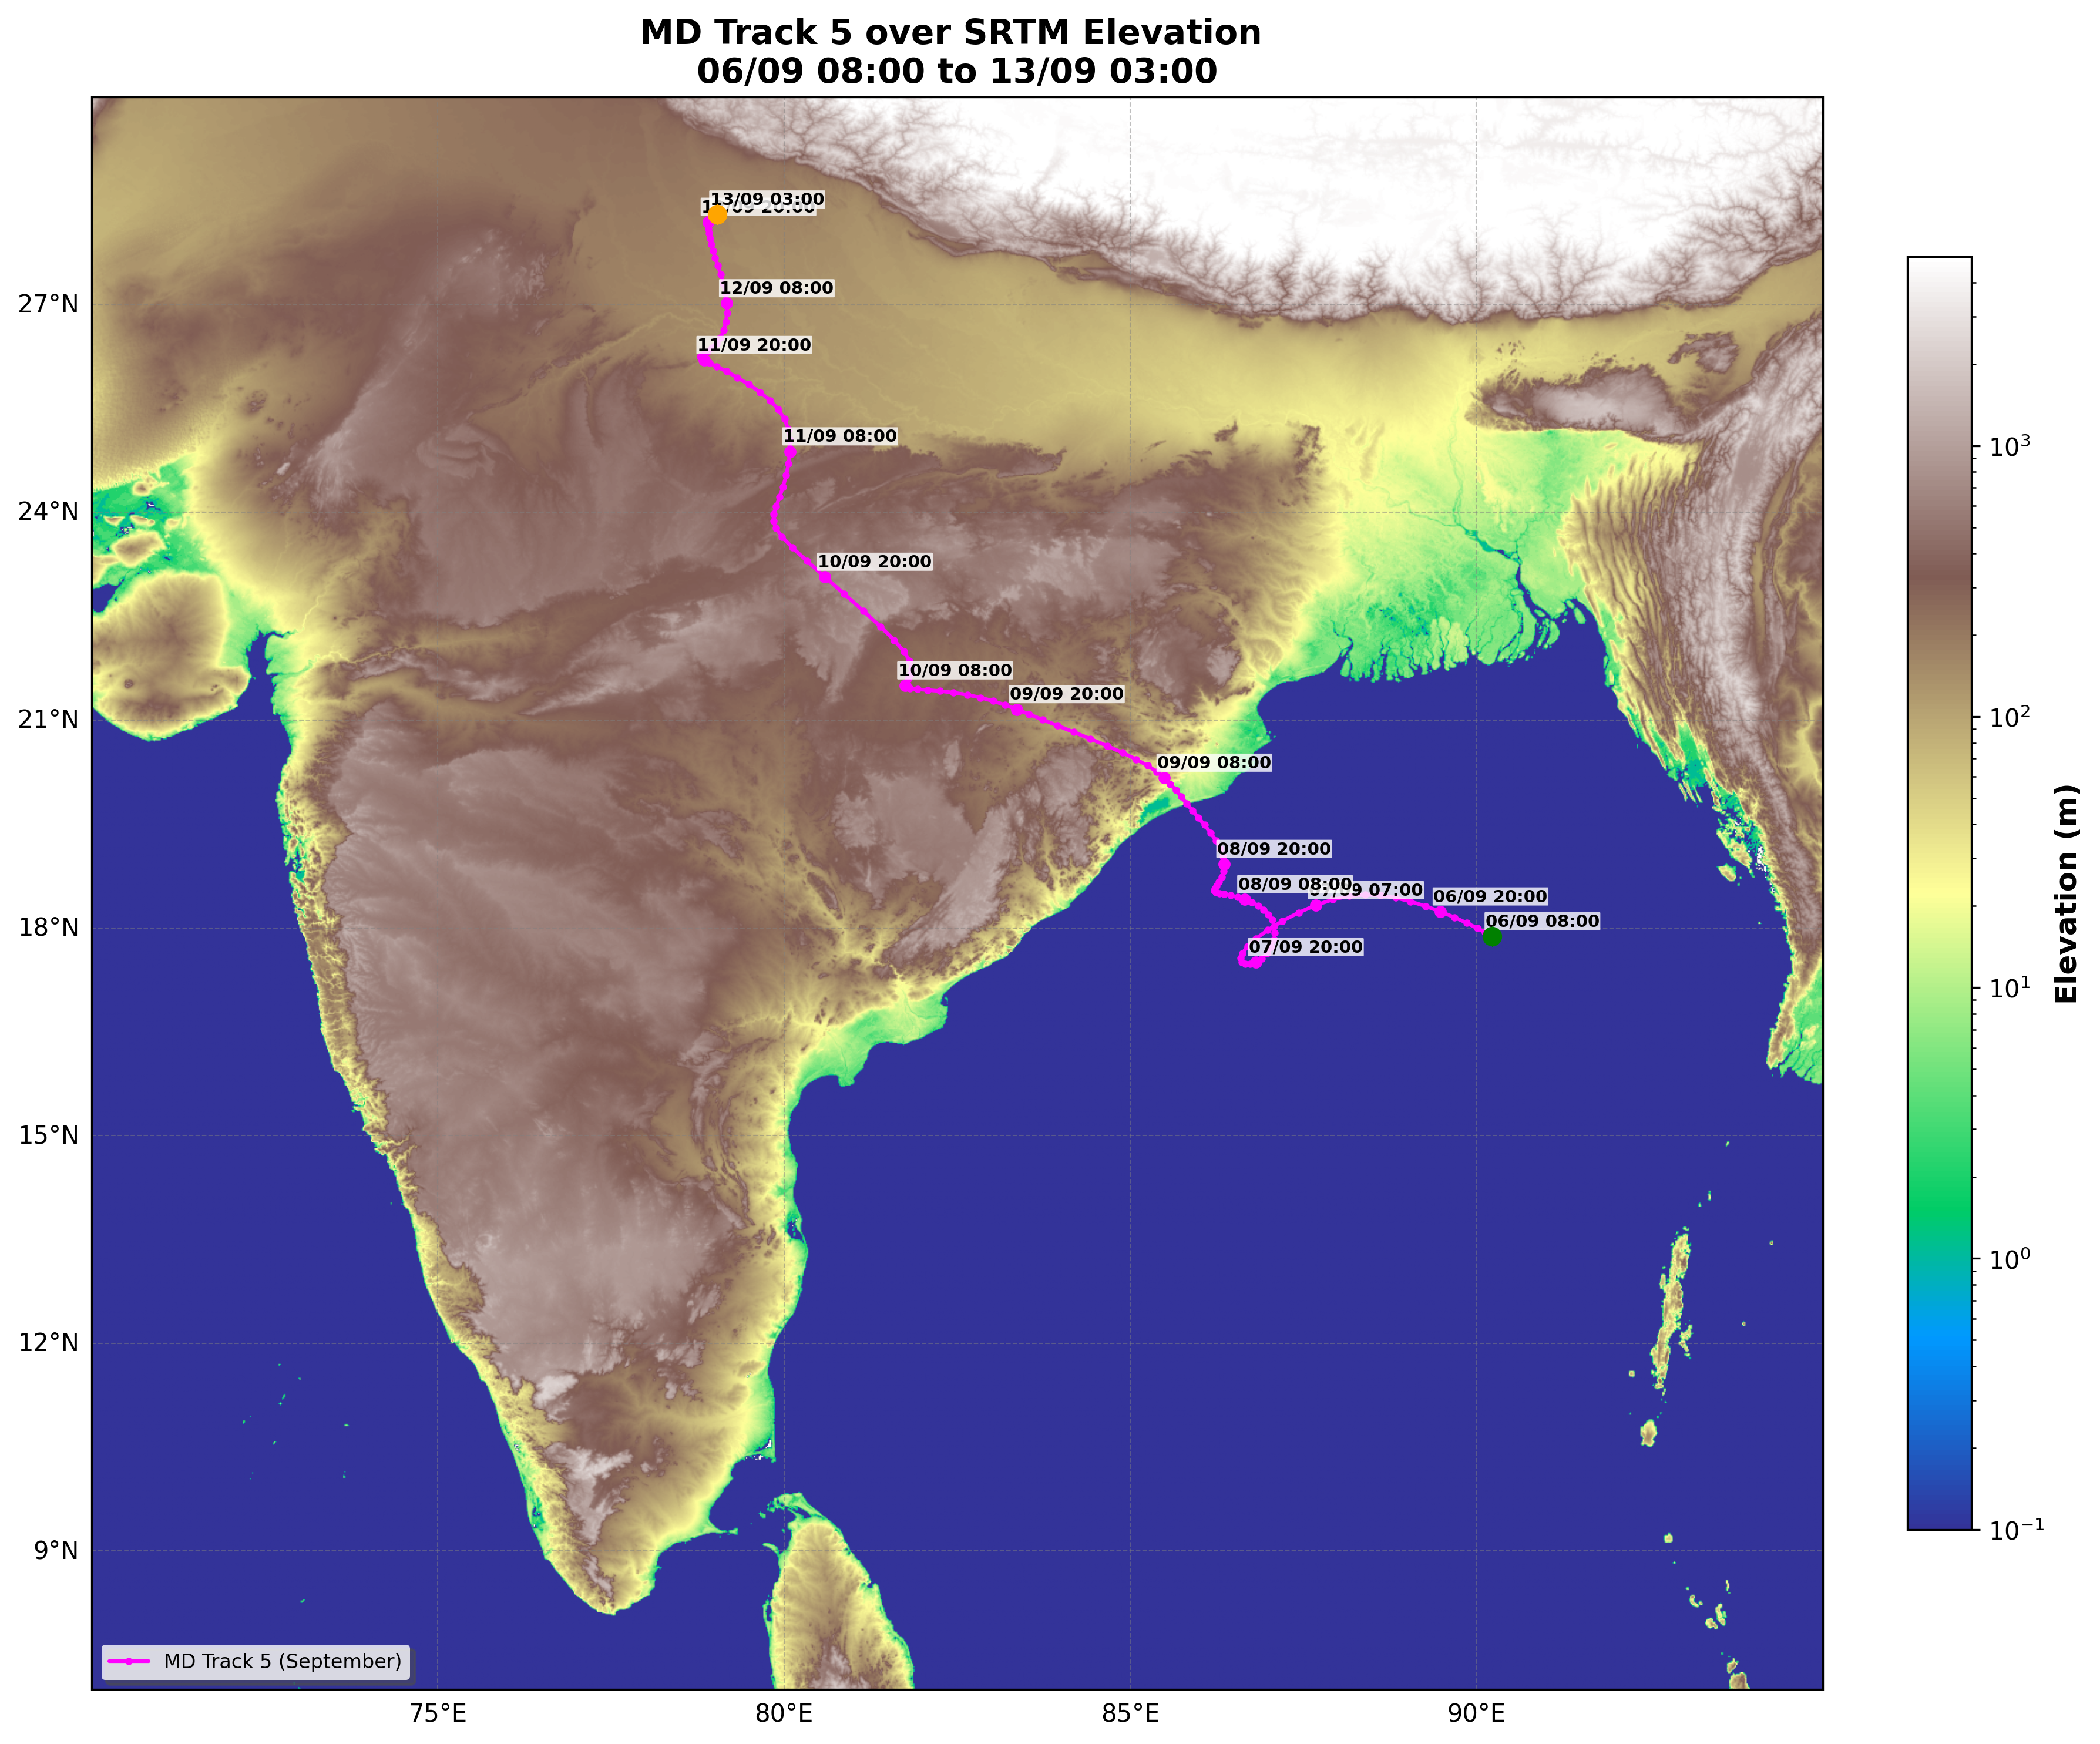
\includegraphics[width=0.85\textwidth]{track_long_elevation_mosaic}
  \caption{BOE-active: Successful terrain crossing and leeward maintenance.}
  \label{fig:long_elevated}
\end{figure}

\begin{figure}[H]
  \centering
  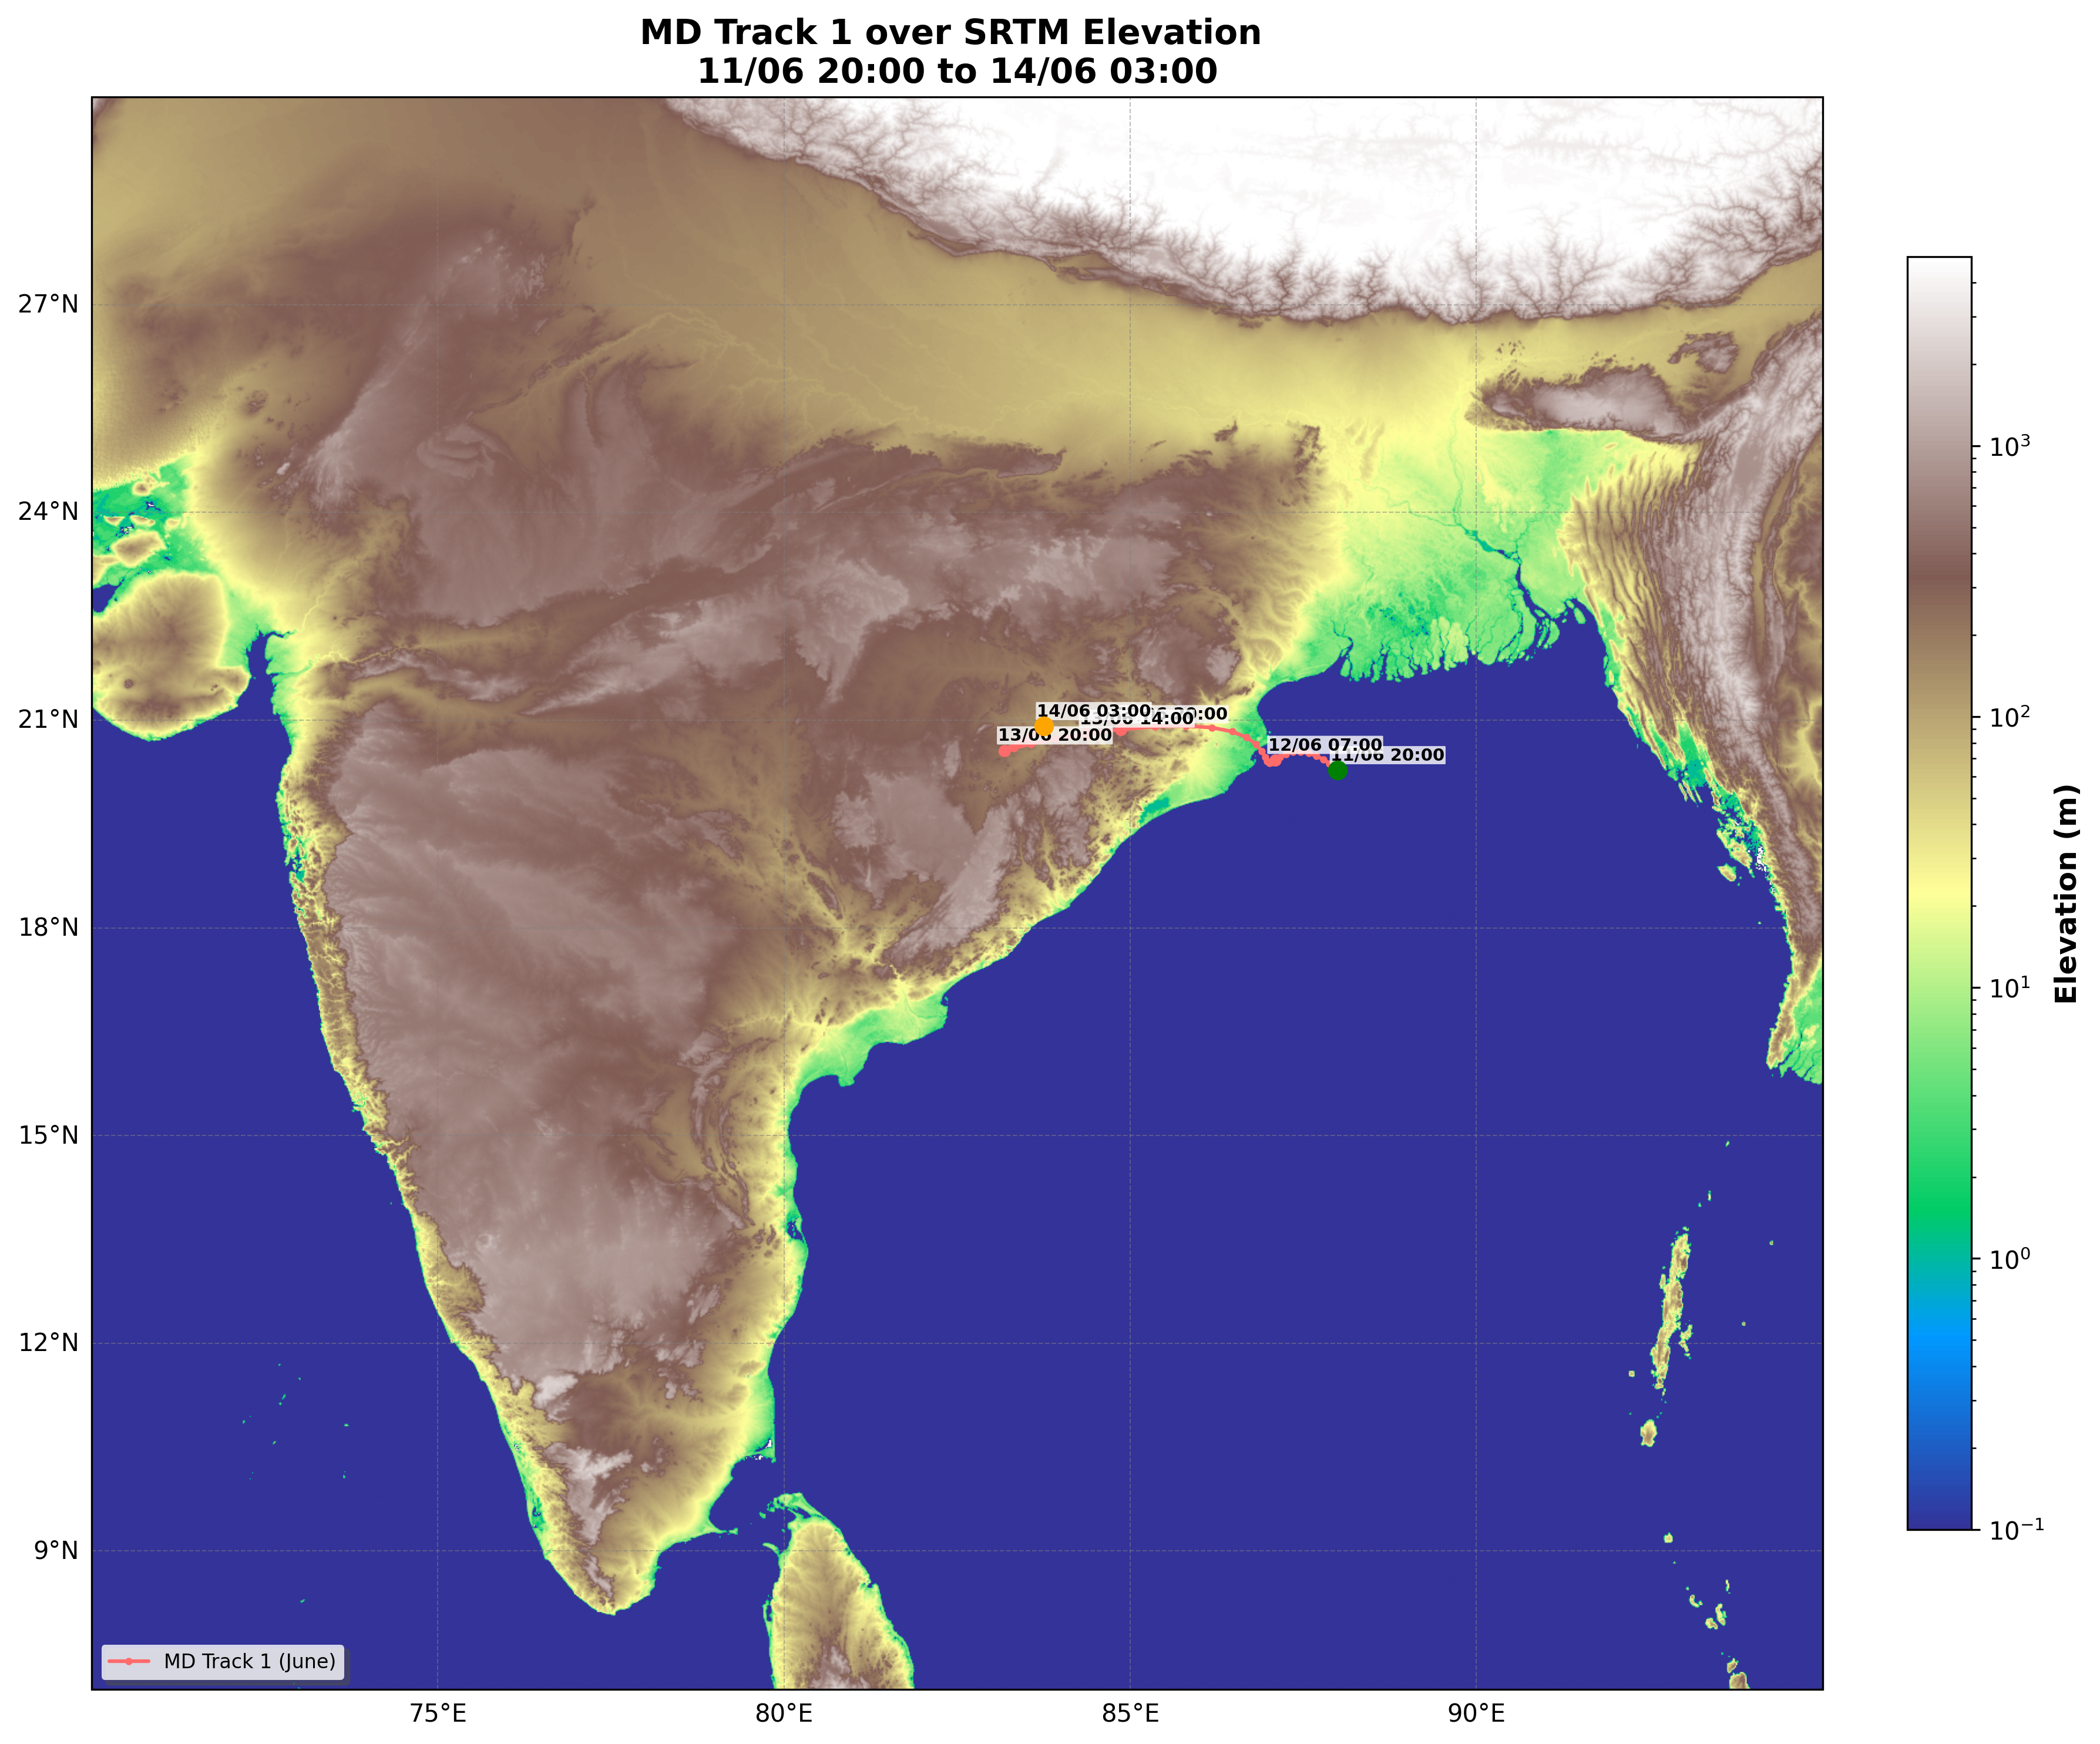
\includegraphics[width=0.85\textwidth]{track_short_elevation_mosaic}
  \caption{Non-BOE: Mechanical dissipation on windward slopes.}
  \label{fig:short_elevated}
\end{figure}

Elevation Mosaic using SRTM data for MD interaction with the Eastern
Ghats. The top panel shows a long-lived track maintaining structural
integrity across high elevation, while the bottom panel illustrates
the typical termination of short-lived systems near the 600\,m contour.

\subsection{Surface Energy Partitioning: LHF and SHF Synchronization}
\label{subsec:ts_hf}

The transition of the surface energy balance at landfall is the
primary determinant of whether a system maintains its oceanic-like
core structure. Figure~\ref{fig:ts_lhf_boe} illustrates the
track-following heat flux evolution for a representative long-lived
(BOE-active) system.

\begin{figure}[H]
  \centering
  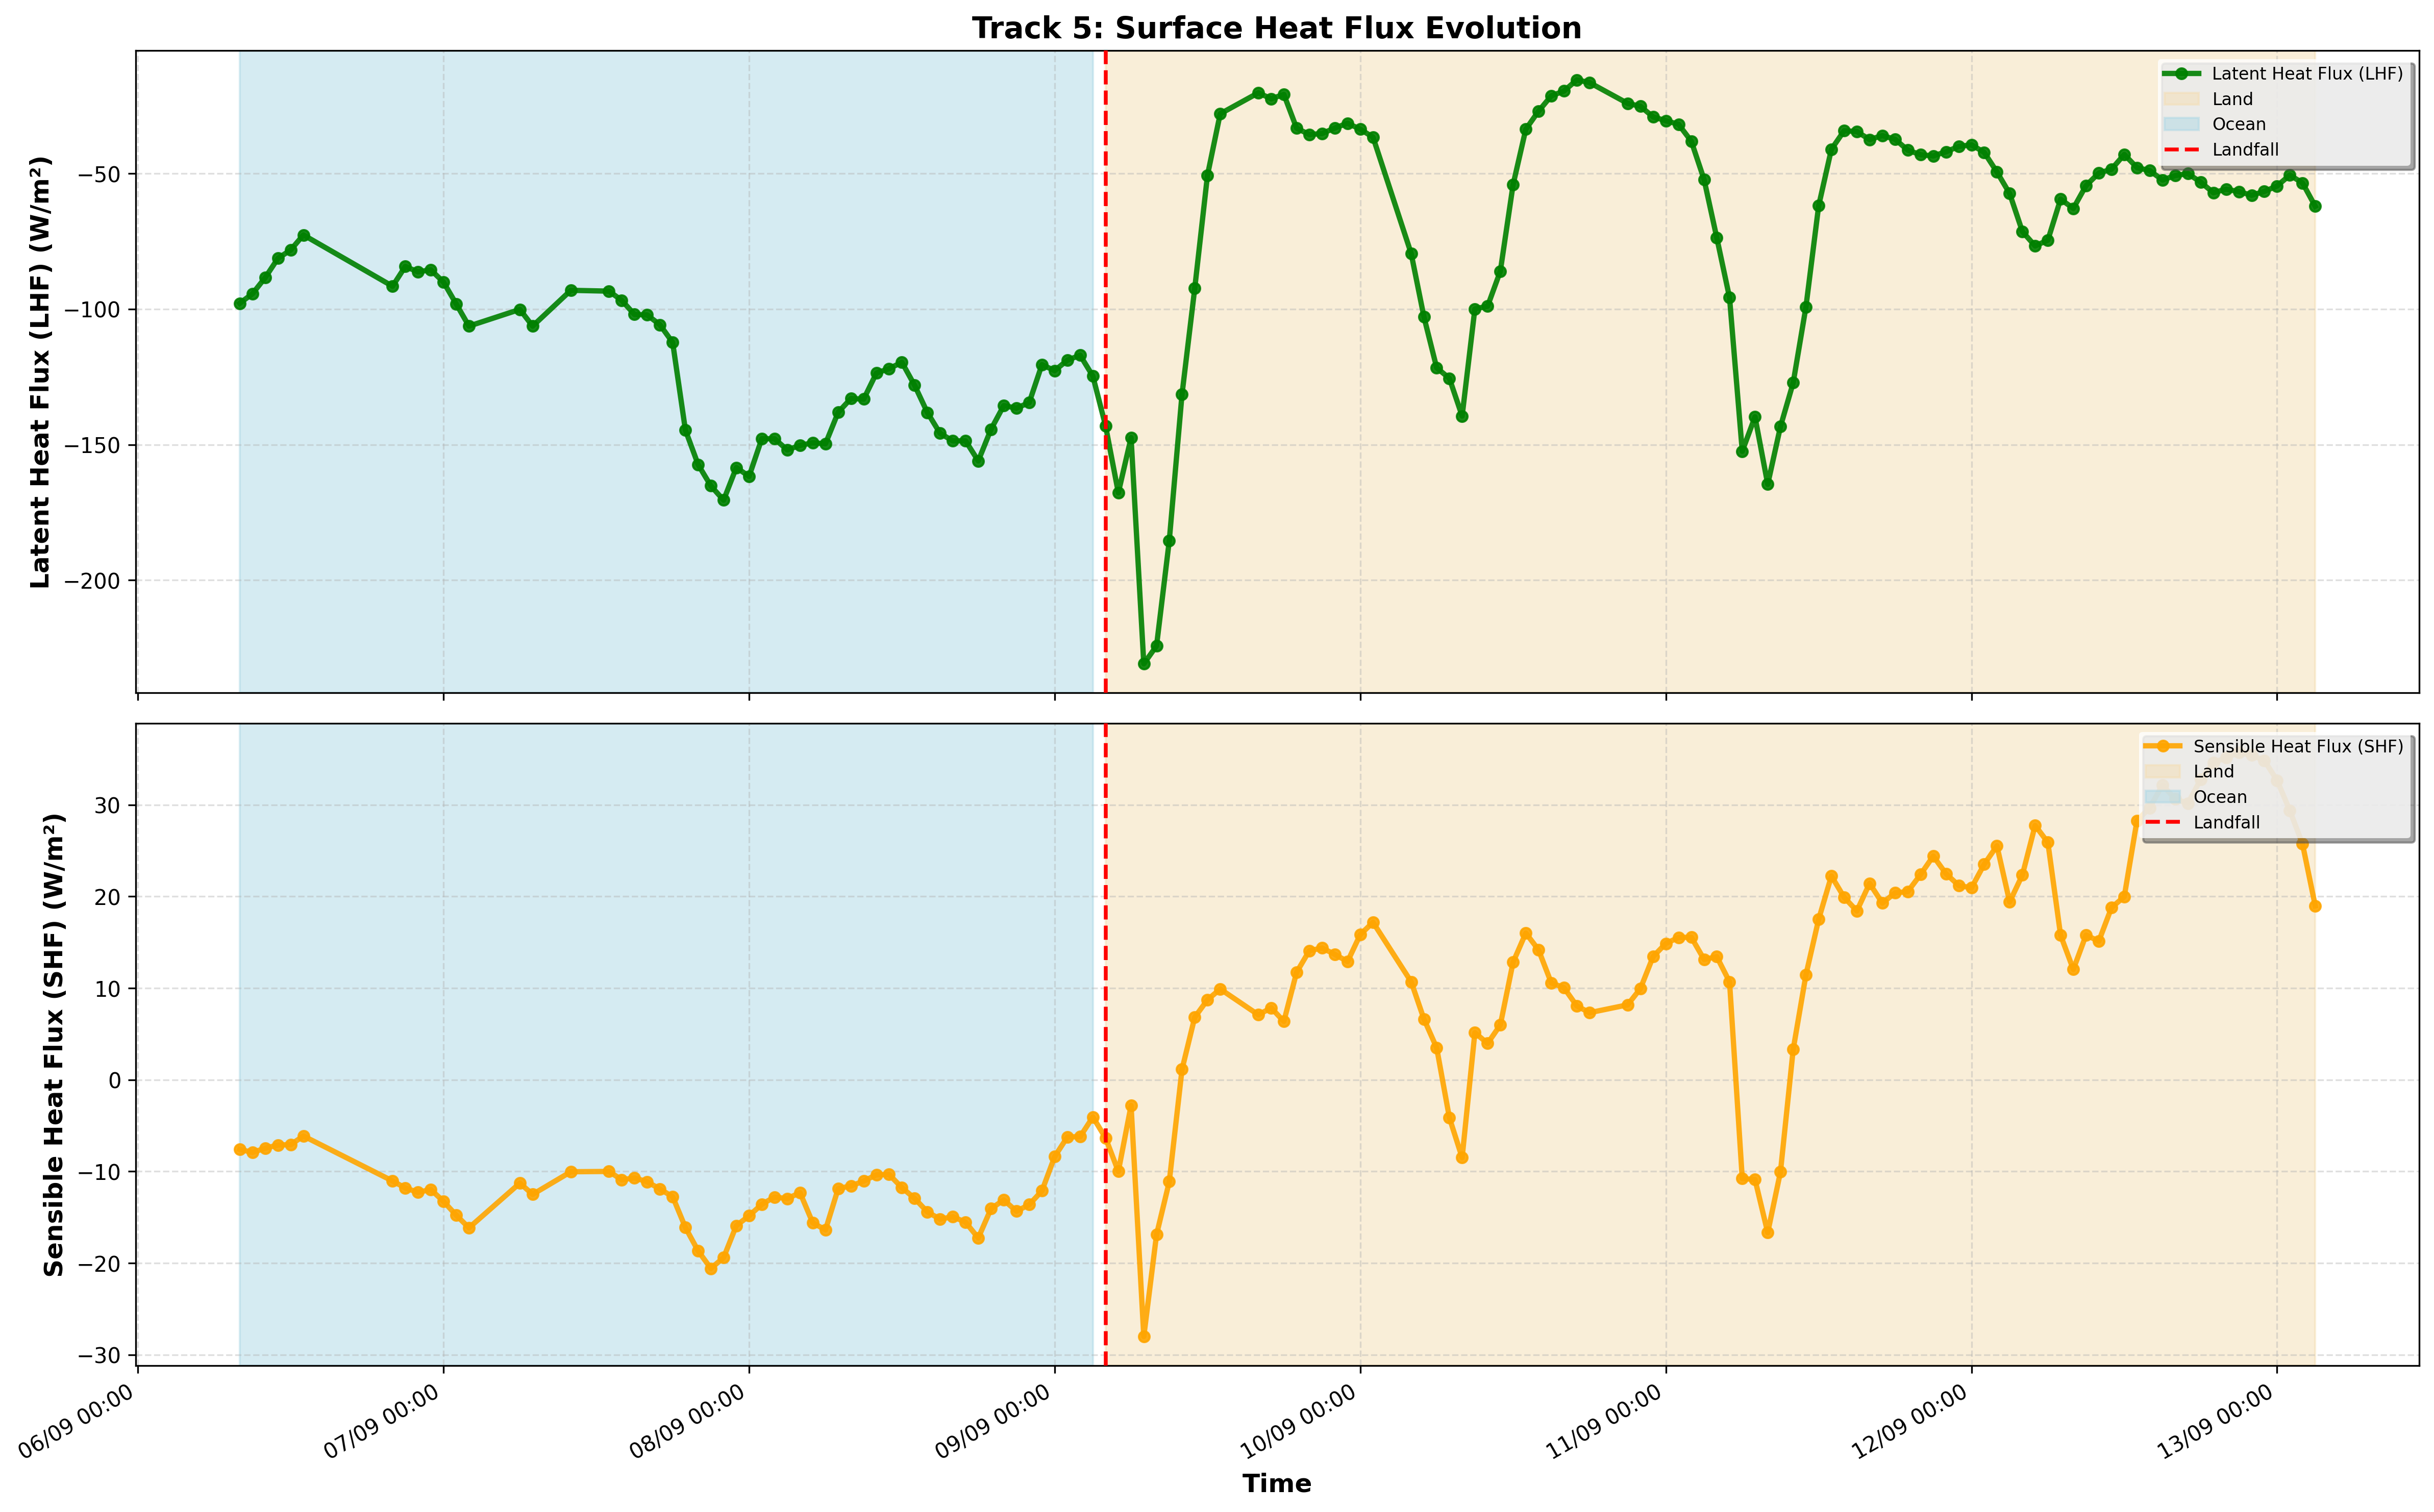
\includegraphics[width=0.9\textwidth]{track_long_HF_time_series}
  \caption{Surface energy fluxes for a long-lived BOE-active MD.
    Continuity of LHF across the landfall boundary and the sustained
  exceedance of the 70\,W\,m$^{-2}$ threshold deep into the land phase.}
  \label{fig:ts_lhf_boe}
\end{figure}

Several thermodynamic features distinguish the BOE-active lifecycle.
\textit{Prior to landfall} ($t < 0$), LHF exceeds
150--200\,W\,m$^{-2}$ while SHF remains near-zero, maintaining the
low-Bowen-ratio state characteristic of the warm Bay of Bengal.
\textit{At landfall} ($t = 0$), the long-lived system exhibits a
resilient energy profile; LHF decreases only modestly and remains
consistently above the 70\,W\,m$^{-2}$ sustaining threshold. This
indicates that the saturated soil acts as an effective surrogate for
the ocean surface. Throughout the land phase ($t > 0$), the system
maintains this high-flux state for over 72~hours, satisfying the
energetic criteria for the Brown Ocean Effect.

In contrast, the short-lived non-BOE population
(Figure~\ref{fig:ts_lhf_nonboe}) displays a fundamental shift in
surface energy partitioning. In these cases, LHF drops below the
critical 70\,W\,m$^{-2}$ threshold within 12--18 hours of landfall.

\begin{figure}[H]
  \centering
  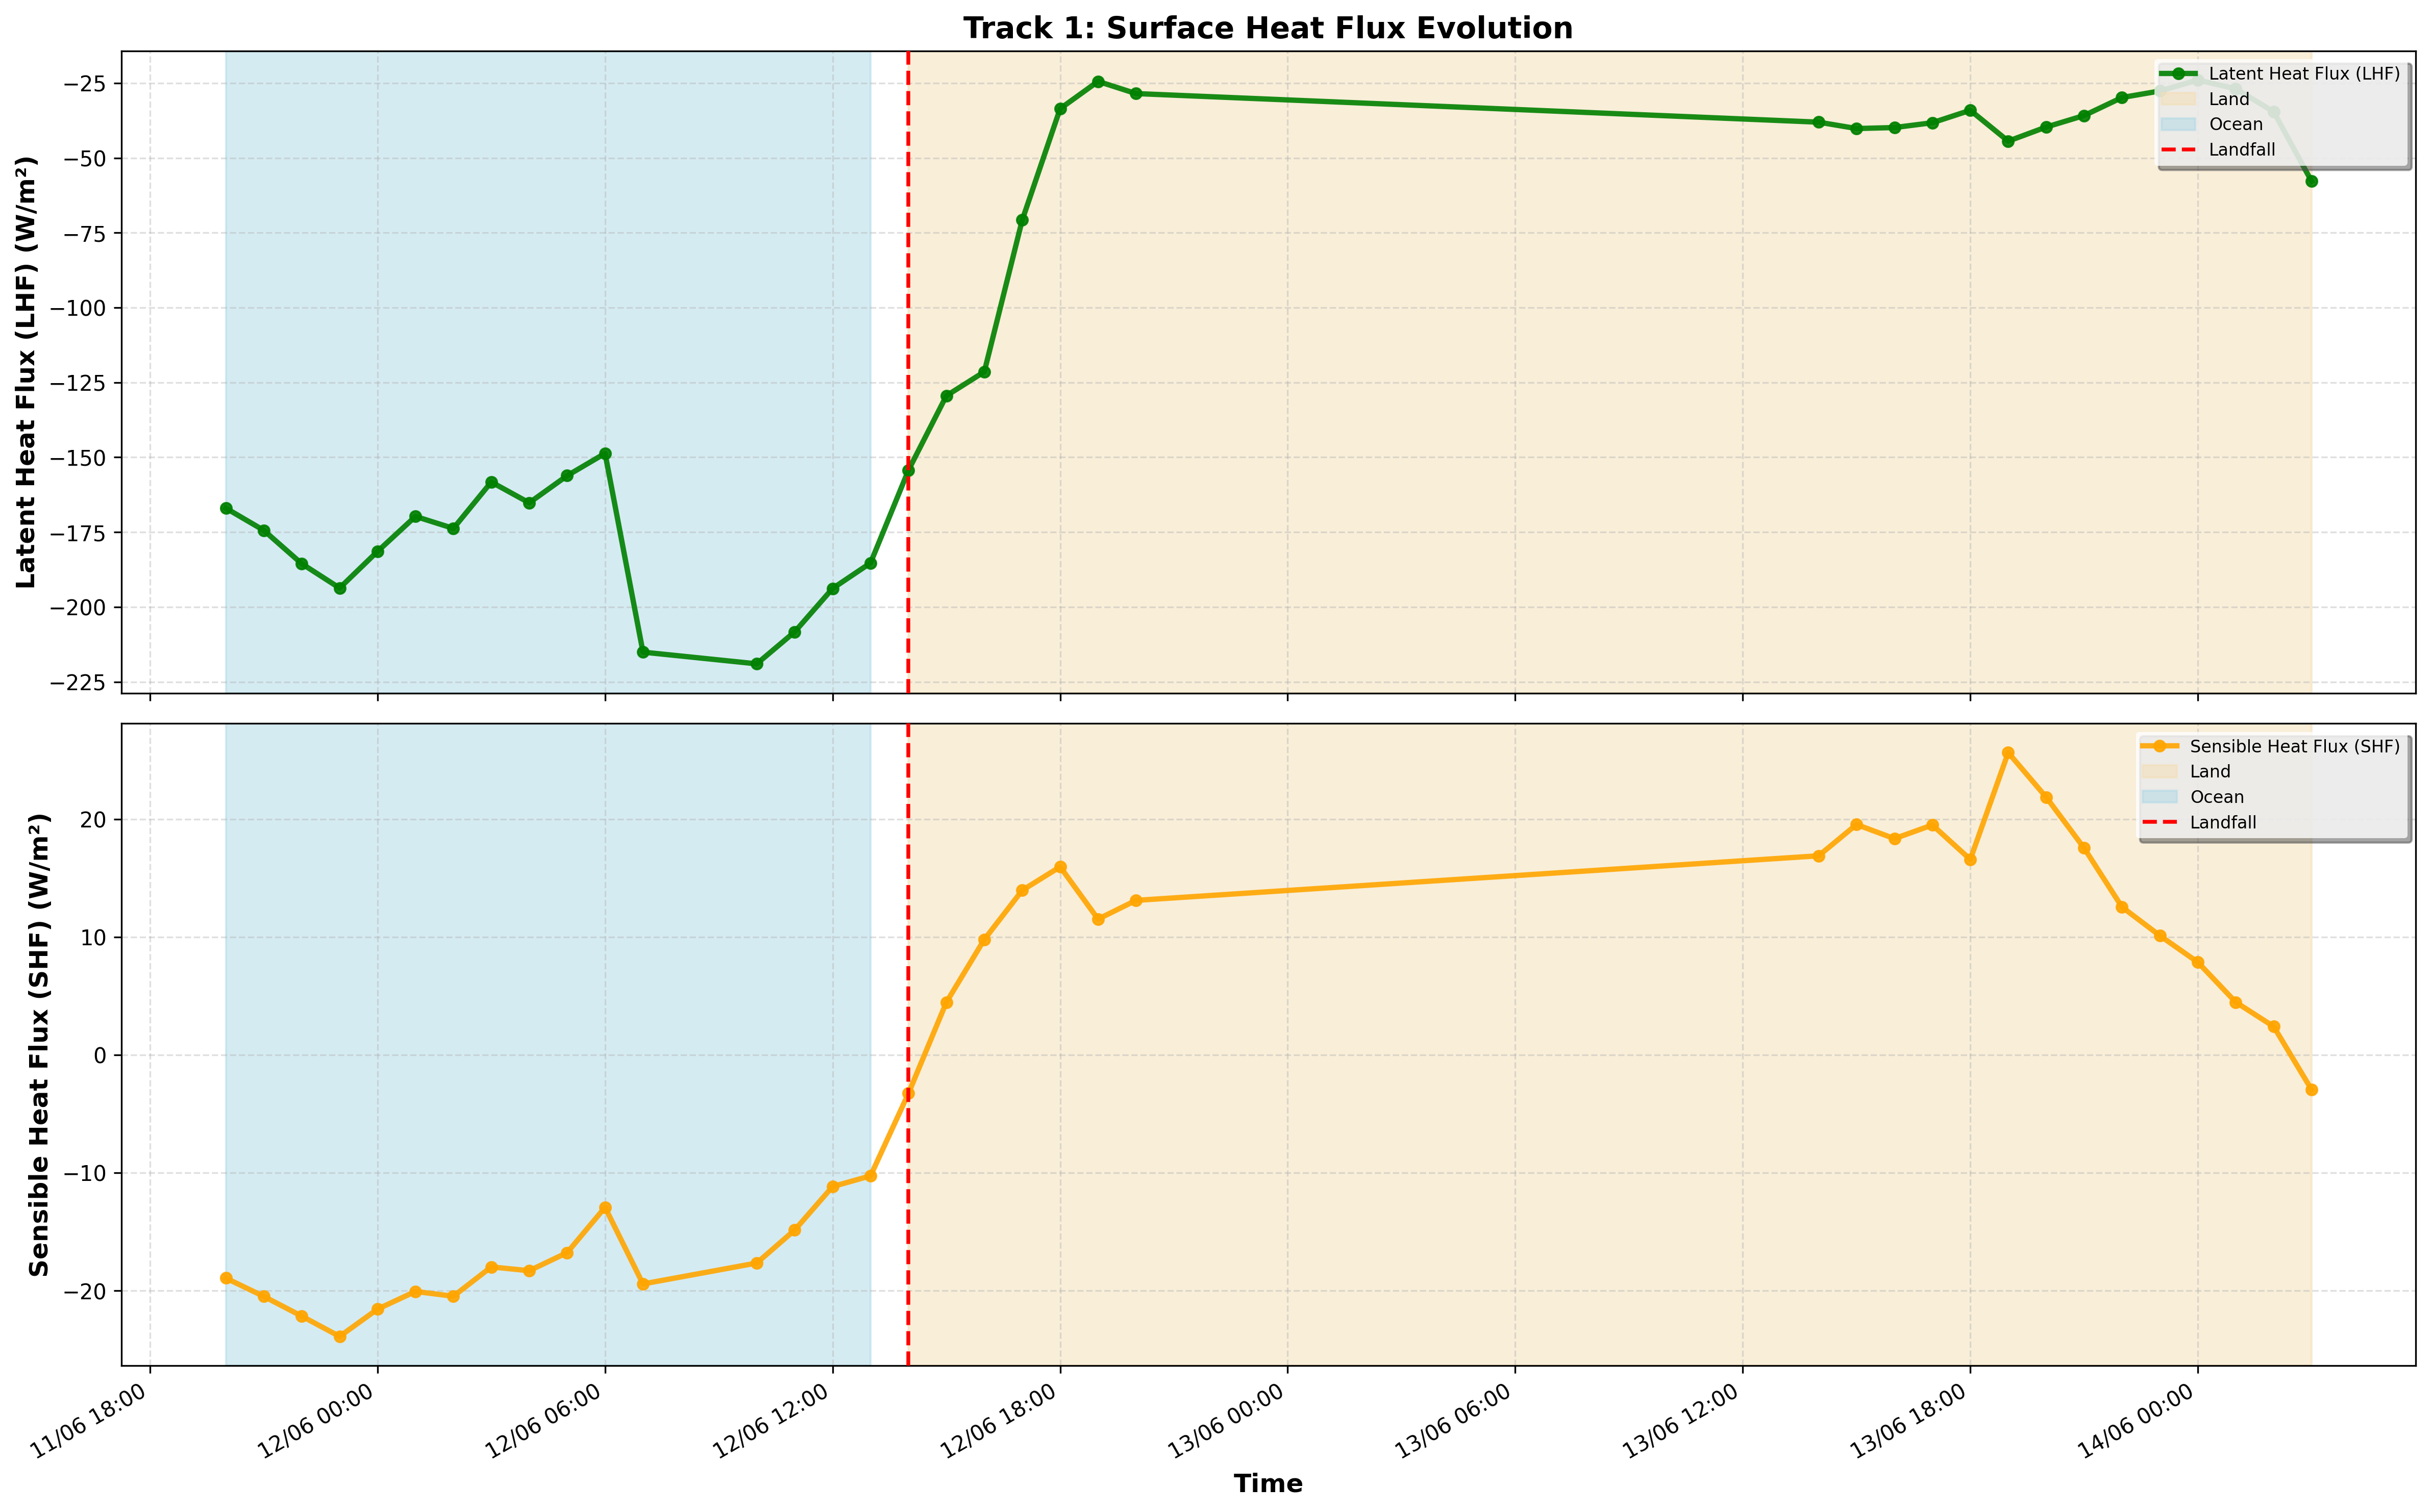
\includegraphics[width=0.9\textwidth]{track_short_HF_time_series}
  \caption{Surface energy fluxes for a short-lived non-BOE MD. The
    rapid collapse of LHF and the corresponding rise in SHF at landfall
  signifies the transition to a water-limited evaporation regime.}
  \label{fig:ts_lhf_nonboe}
\end{figure}

Simultaneously, the SHF in short-lived systems rises sharply to
values exceeding 30--40\,W\,m$^{-2}$. This transition from a latent
dominated to a sensible-dominated regime marks the shift from an
energy-limited to a water-limited surface \autocite{seneviratne2010investigating}.
Physically, this means the surface energy is no longer being utilized
to recycle moisture into the MD's core, but is instead heating the
boundary layer, which encourages dry-air entrainment and triggers
the rapid structural collapse observed in Section~\ref{subsec:hovmoller_tp}.

\subsection{Feedback: The Precipitation-Soil Moisture Loop}
\label{subsec:ts_sm_tp}

The integration of heat flux diagnostics with the temporal evolution
of moisture confirms the existence of a closed-loop feedback in
BOE-active systems. While the Hovm\"{o}ller analysis captures the
radial contraction of the MD, the track-following time-series
(Figures~\ref{fig:long_ts_sm_tp} and \ref{fig:short_ts_sm_tp})
reveals the temporal synchronization required for inland maintenance.

\subsubsection*{Self-Wetting Dynamics in BOE-Active Systems}

Figure~\ref{fig:long_ts_sm_tp} illustrates the co-evolution of
\texttt{swvl1} and total precipitation (\texttt{TP}) for a
representative long-lived MD. Three temporal features define the BOE
maintenance phase:
\begin{enumerate}
  \item \textbf{Pre-conditioned Landfall ($t=0$):} The system
    encounters antecedent soil moisture levels already $\geq
    0.35$\,m$^3$\,m$^{-3}$. This high initial state prevents the
    standard surface energy collapse associated with dry-landfall.
  \item \textbf{The Intensive Wetting Phase ($0 < t < 36$\,h):}
    Post-landfall, \texttt{swvl1} rises progressively toward field
    capacity ($\sim 0.46$\,m$^3$\,m$^{-3}$). This rise is driven by
    the MD's own inner-core precipitation, which remains sustained
    around 4\,mm\,h$^{-1}$.
  \item \textbf{Phase Synchronization:} The simultaneous maintenance
    of heavy precipitation while \texttt{swvl1} approaches saturation
    confirms a positive feedback loop. The storm's rainfall sustains
    the soil reservoir, which in turn fuels the LHF
    ($>70$\,W\,m$^{-2}$) necessary to drive subsequent deep convection.
\end{enumerate}

\begin{figure}[H]
  \centering
  \includegraphics[width=0.98\textwidth]{track_long_tp-swvl1_time_series}
  \caption[Co-evolution of Soil moisture (\texttt{SWVL1}) and Total
  precipitation (\texttt{TP}), BOE-active MD]{Track-following Soil
    moisture \texttt{SWVL1} and Total precipitation (\texttt{TP}) for a
    long-lived MD. The sustained precipitation concurrent with rising
  soil moisture indicates the establishment of a self-wetting feedback loop.}
  \label{fig:long_ts_sm_tp}
\end{figure}

\subsubsection*{Feedback Failure in Short-Lived Systems}

For comparison, the non-BOE system (Figure~\ref{fig:short_ts_sm_tp})
exhibits a failure to establish this feedback. Although the system
may produce an initial burst of precipitation at landfall, the lack
of pre-conditioned soil leads to rapid surface desiccation. Without
the moisted land surface provided by high antecedent soil moisture, the
LHF collapses (as seen in Section~\ref{subsec:ts_hf}), causing the
precipitation to cease before the soil can reach a sustaining level
of saturation. This confirms that the BOE is a threshold-gated
mechanism; if the self-wetting loop is not activated within the first
24 hours of landfall, the system inevitably undergoes structural decay.

\begin{figure}[H]
  \centering
  \includegraphics[width=0.98\textwidth]{track_short_tp-swvl1_time_series}
  \caption[Co-evolution of Soil moisture (\texttt{SWVL1}) and
  precipitation (\texttt{TP}), Non-BOE MD]{Track-following
    \texttt{swvl1} and precipitation for a short-lived MD. The rapid
    decline in precipitation at $t \approx 18$\,h prevents the soil
    from reaching field capacity, resulting in the dissipation of the
  surface energy reservoir.}
  \label{fig:short_ts_sm_tp}
\end{figure}

% \subsection{Bowen Ratio: Quantifying Evaporation}
% \label{subsec:ts_bowen}
%
% From Figure~\ref{fig:ts_bowen}, the Bowen ratio trajectory isolates
% the transition most clearly. Over the ocean ($t < 0$), both
% long-lived and short-lived categories show $\beta \approx
% 0.2$-$0.3$, the characteristic low Bowen ratio of a moisture-rich
% surface. At landfall, the divergence between the two populations is
% immediate and quantitatively large. For BOE candidates, $\beta$
% rises only to $\approx 0.4$-$0.5$, confirming that the surface
% remains in the energy-limited evaporation throughout the land
% phase: evaporation is limited not by water supply but by the
% available radiative energy. For non-BOE systems, $\beta$ rises
% steeply, exceeding 1.0 within \textbf{[T\_beta1]}\,hours of
% landfall, meaning sensible heating has overtaken latent heating. A
% $\beta > 1.0$ implies the surface is actively heating the boundary
% layer while providing insufficient moisture flux to sustain
% convective instability-a state incompatible with continued MD organisation.
%
% %%  FIGURE: Bowen ratio comparison
% %%  SOURCE: output_YYYY/track_N/time_series/track_N_bowen_ratio.png
% %%  Overlay BOTH long-lived (orange) and short-lived (blue) on same axes.
% %%  Add reference lines at beta = 0.3 (oceanic value) and beta = 1.0 (parity).
% \begin{figure}[H]
%   \centering
%   %% >> INSERT FIGURE: overlay of BOE-candidate and non-BOE Bowen
% ratio plots <<
%   \fbox{\rule{0pt}{6cm}\rule{0.85\textwidth}{0pt}}
%   % \includegraphics[width=0.85\textwidth]{bowen_ratio_comparison}
%   \caption[Track-following Bowen ratio time series]{Bowen ratio
%     ($\beta = Q_H/Q_E$)
%     for long-lived BOE-candidate (orange) and short-lived non-BOE (blue) MDs.
%     Reference lines at $\beta = 0.3$ (oceanic value) and $\beta =
% 1.0$ (LHF/SHF
%     parity). The divergence after $t = 0$ reflects fundamentally
%     different post-landfall
%   surface energy regimes.}
%   \label{fig:ts_bowen}
% \end{figure}

\subsection{Translational Speed: Terrain Deceleration and BOE Recovery}
\label{subsec:ts_speed}

The interaction between the MD core and the complex orography of the
Eastern Ghats is most clearly visible in the evolution of
translational speed ($V_t$). As shown in the elevation-speed maps
(Figures~\ref{fig:track_long_speed_map} and
\ref{fig:track_short_speed_map}), elevation acts as a mechanical sink
for the system's kinetic energy.

\textit{Over the ocean}, MDs translate at a steady mean speed of
6\,m\,s$^{-1}$. However, as the systems encounter the 200-1000\,m
elevation gradient of the Eastern Ghats, both MDs undergo significant
deceleration. This is consistent with increased surface roughness and
mechanical flow blocking \autocite{houze1994}, which reduces the
low-level momentum of the vortex.

The critical divergence occurs west of the main terrain crest.
Long-lived (BOE-active) systems exhibit a clear leeward speed
recovery; as elevation drops below 200\,m, the speed returns to
approximately 5\,m\,s$^{-1}$. This suggests that the sustained
surface LHF (the BOE engine) maintains the low-level pressure
gradient force required to drive the system forward.

Conversely, short-lived systems fail to overcome the mechanical drag
by elevated land. In Figure~\ref{fig:track_short_speed_map}, these
tracks often show a stalling behavior or a slight recurvature before
dissipating. Without the thermodynamic replenishment from the soil,
the convective MD vortex structure collapses during the
terrain-crossing phase, leading to a permanent loss of translational
momentum and subsequent track termination.

\begin{figure}[H]
  \centering
  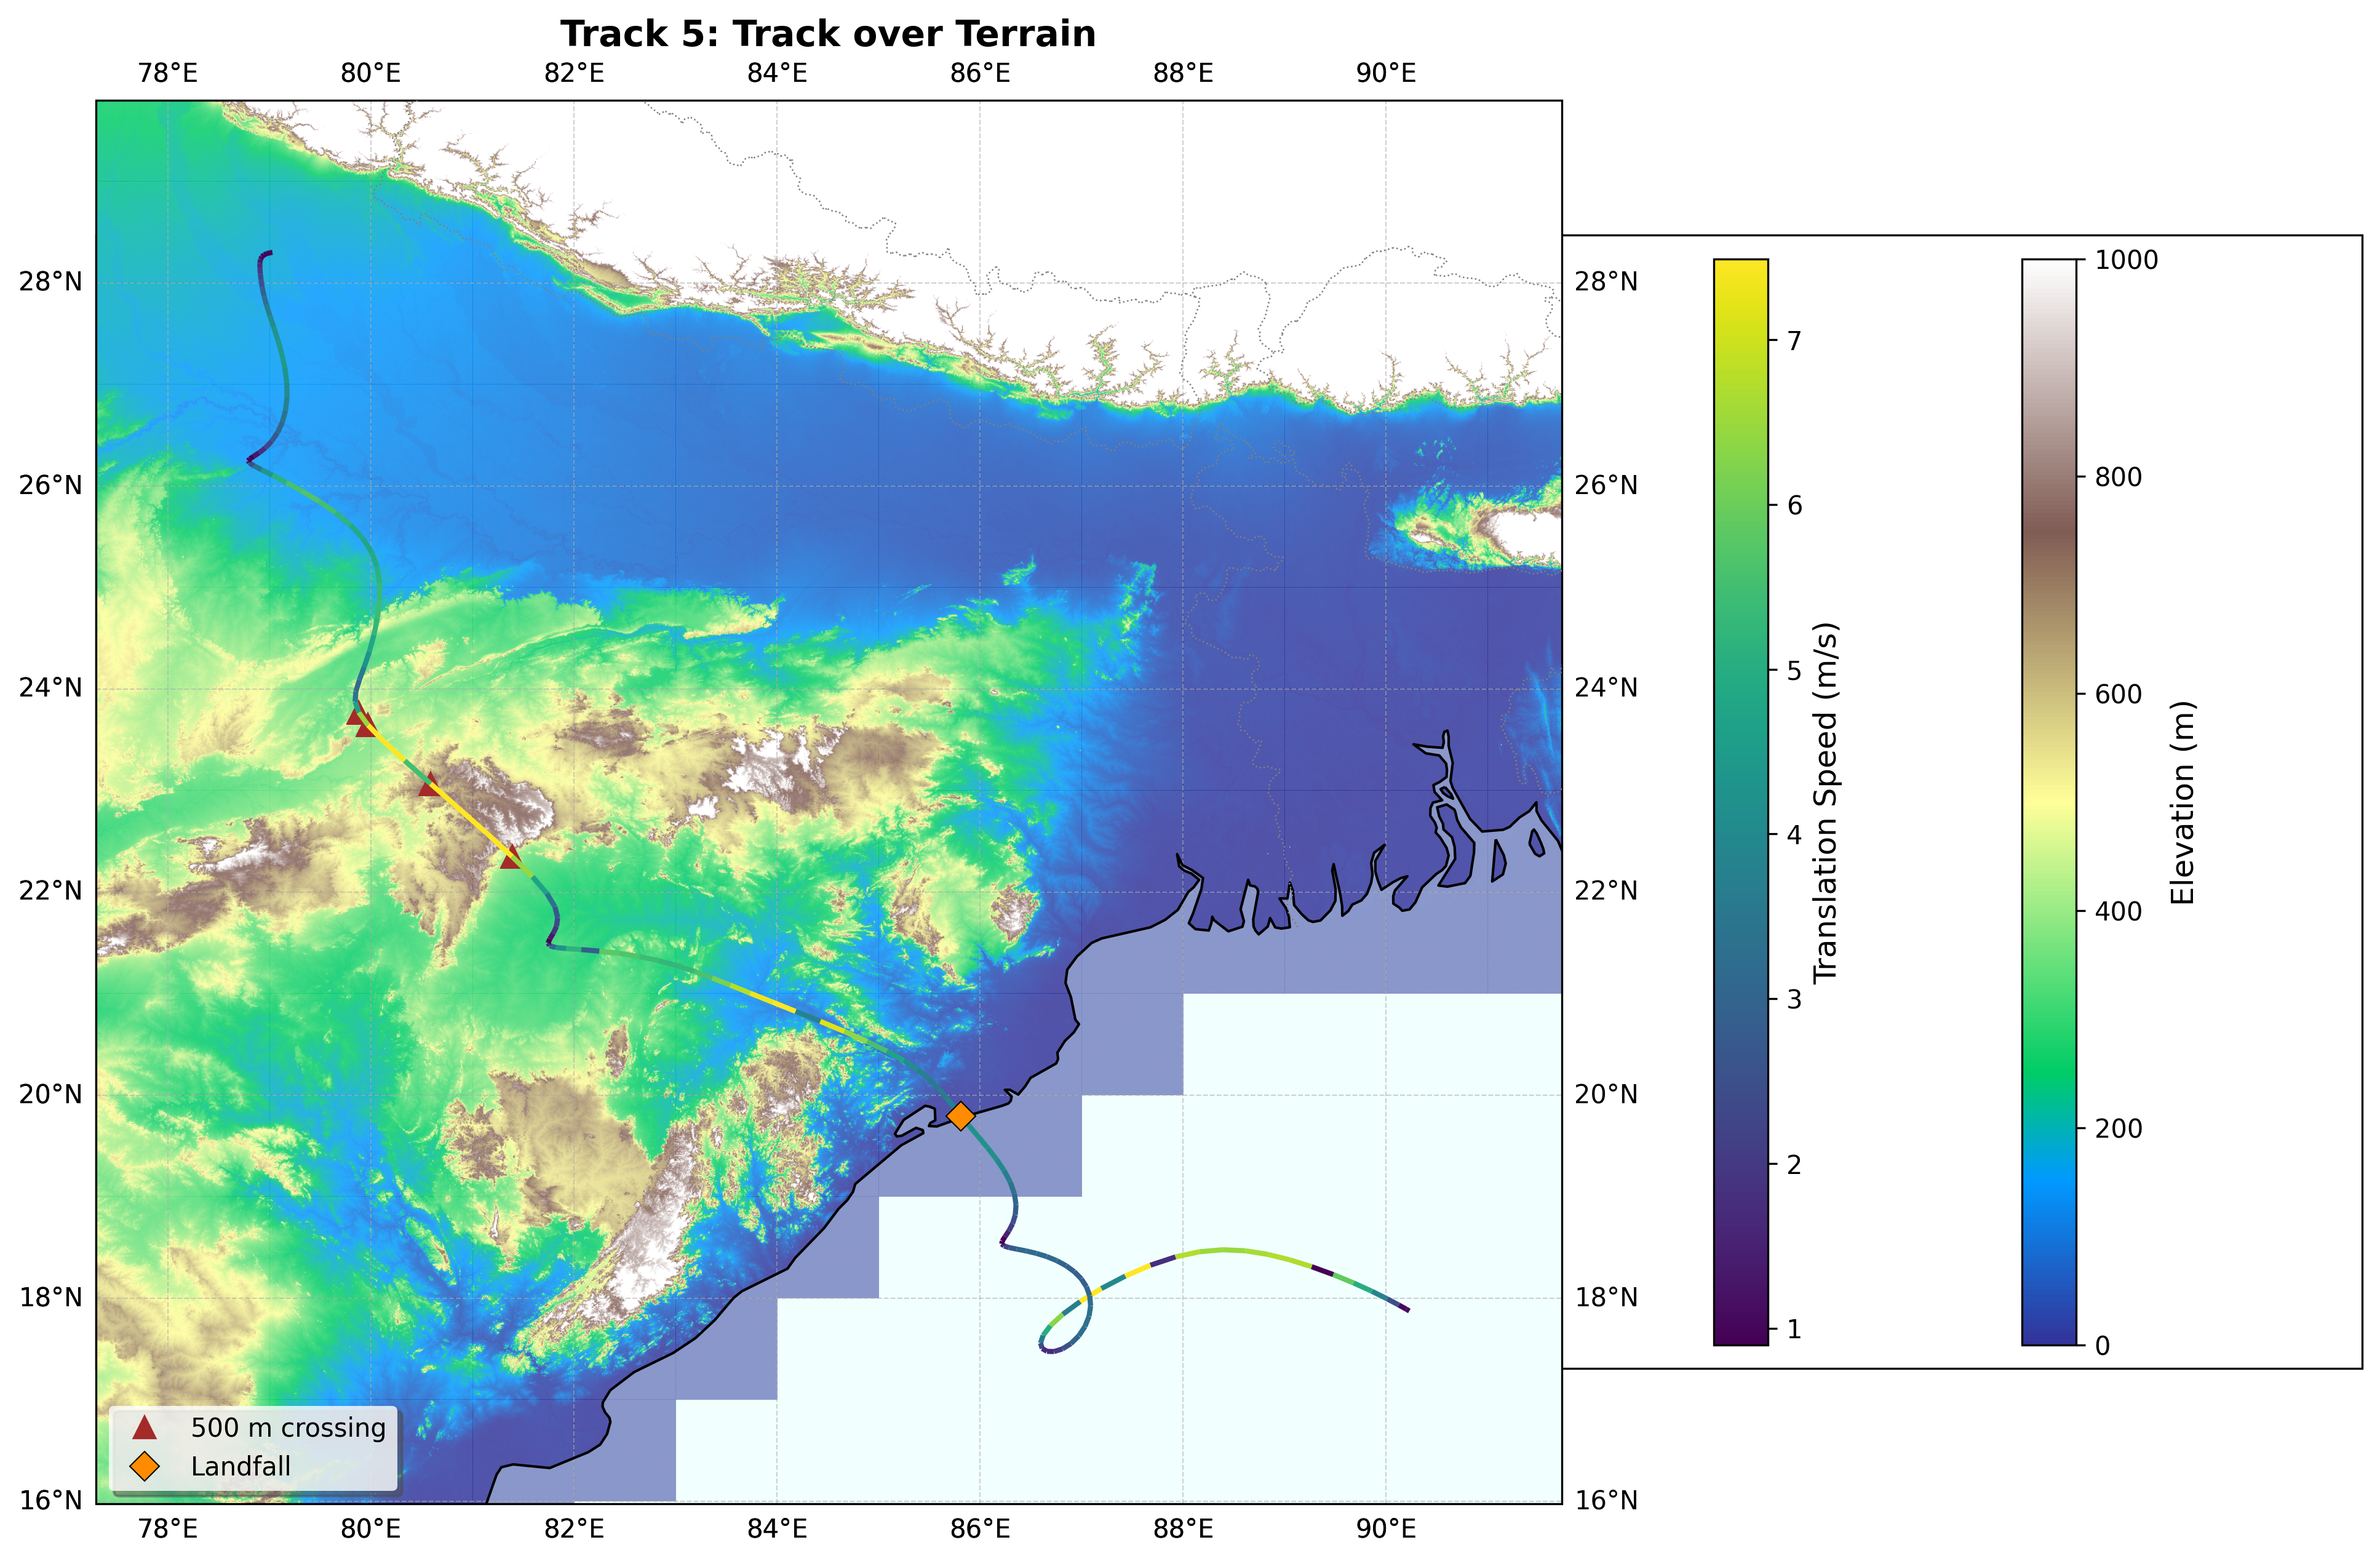
\includegraphics[width=0.86\textwidth]{track_long_elevation_speed_map}
  \caption{BOE-active: Speed recovery following the crossing of the
  600\,m contour.}
  \label{fig:track_long_speed_map}
\end{figure}

\begin{figure}[H]
  \centering
  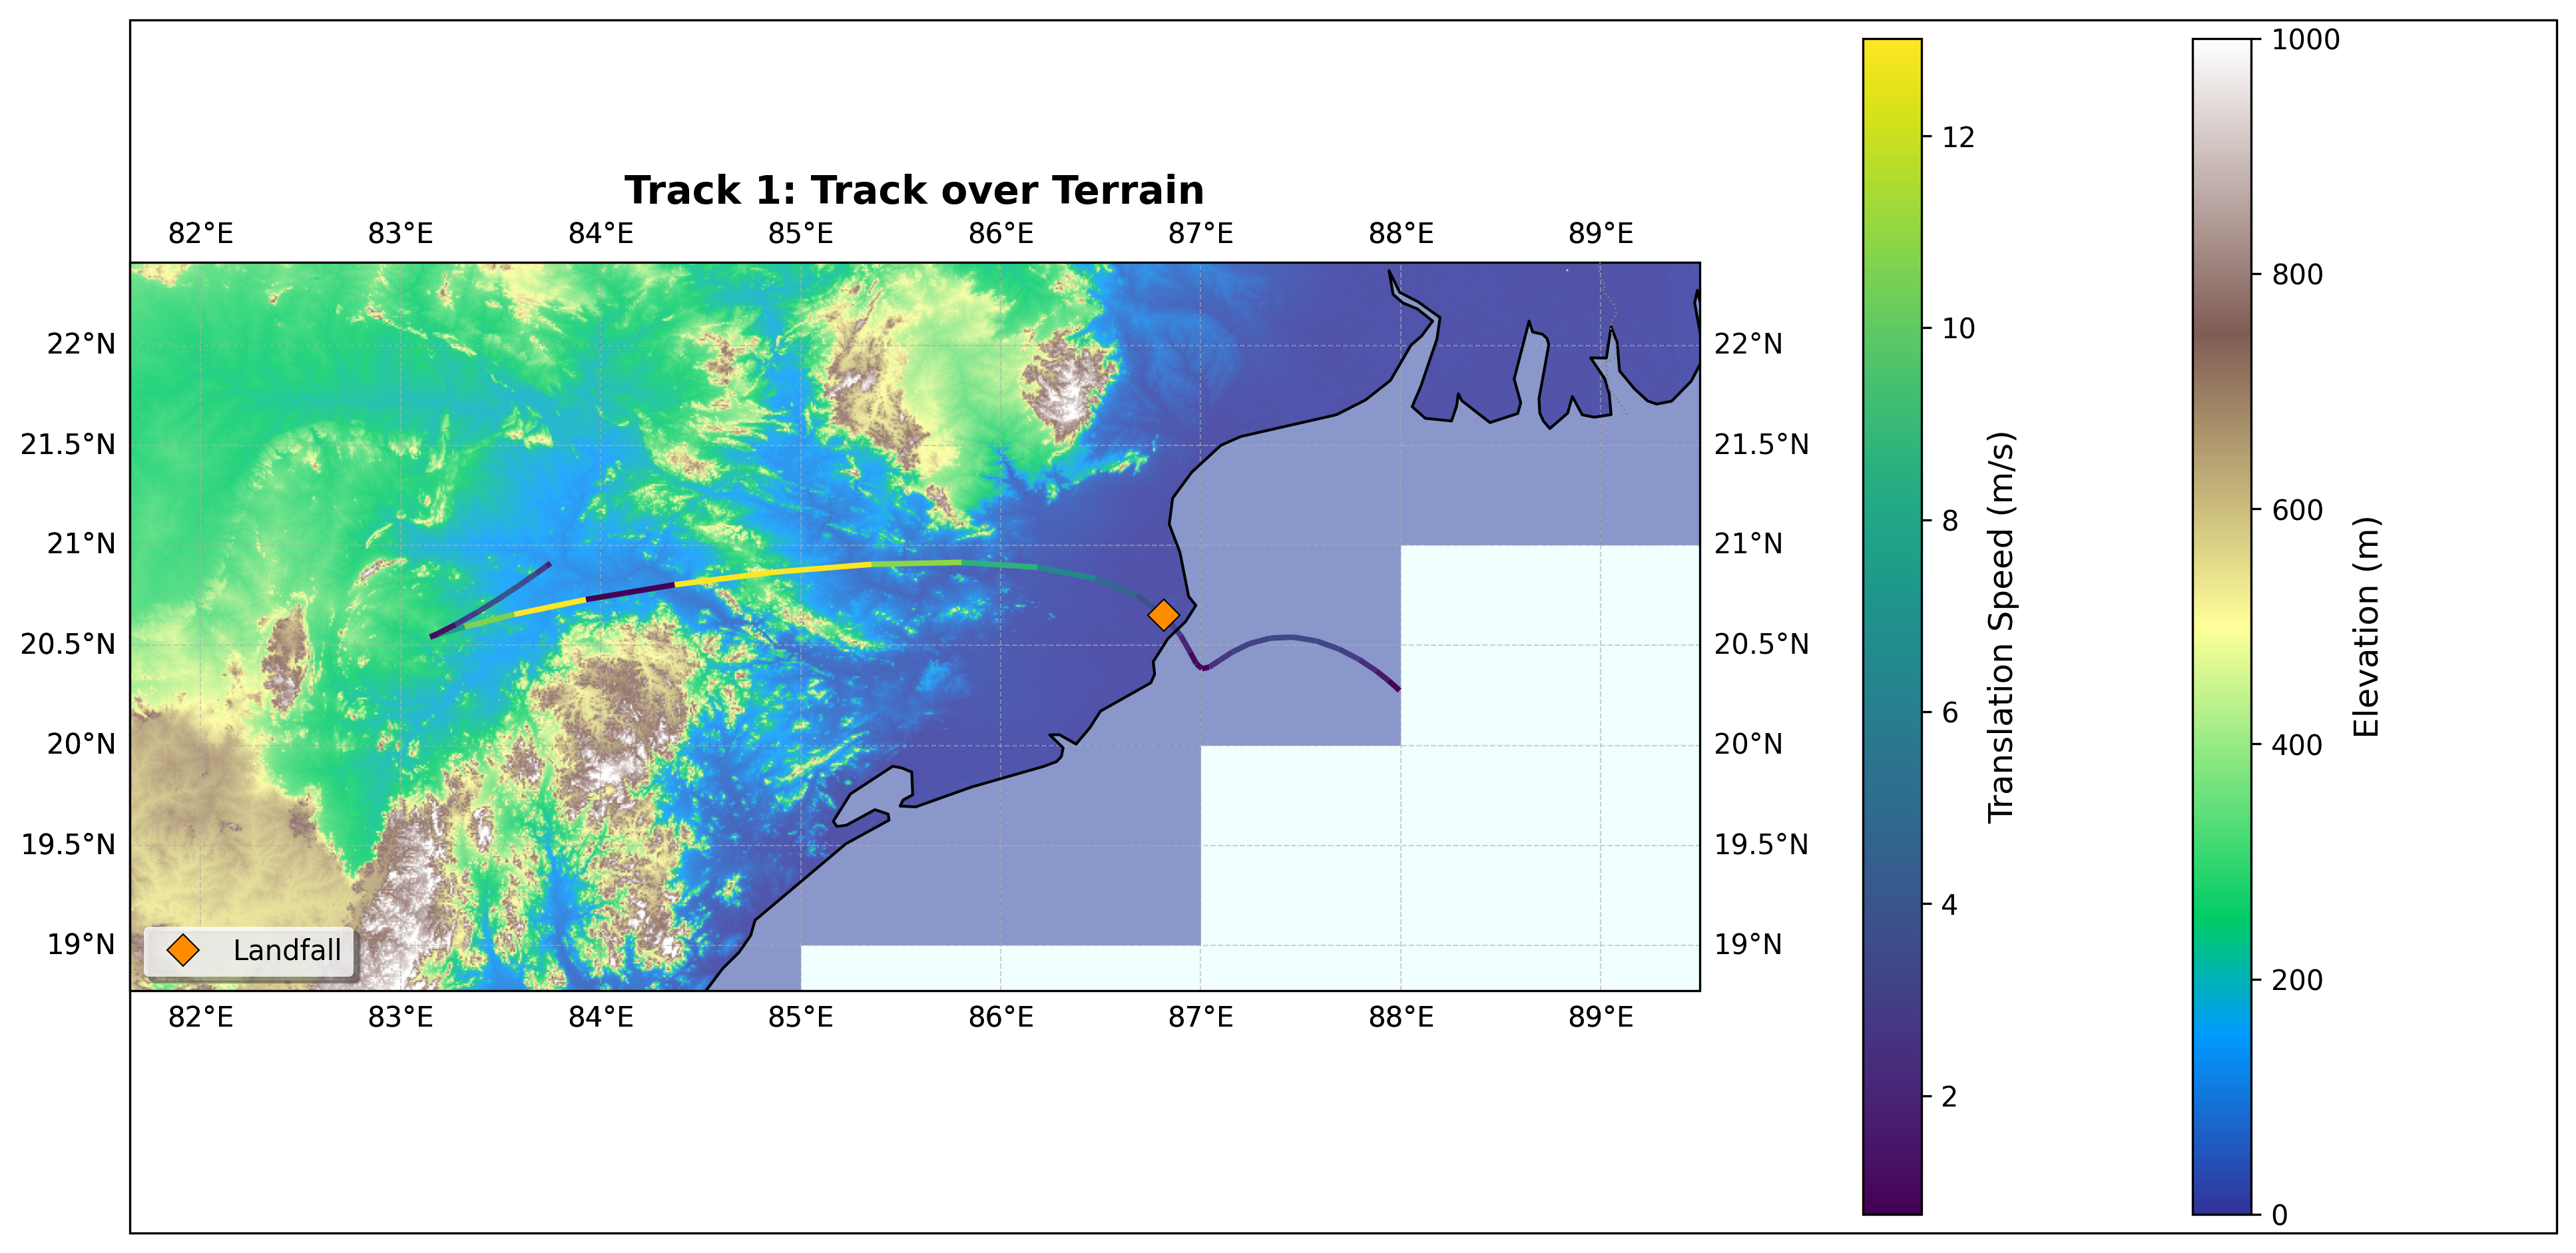
\includegraphics[width=0.86\textwidth]{track_short_elevation_speed_map}
  \caption{Non-BOE: Sustained deceleration and track termination
  upon terrain encounter.}
  \label{fig:track_short_speed_map}
\end{figure}

Spatial evolution of MD translational speed overlaid on SRTM
elevation. While both systems decelerate upon landfall, the
long-lived system exhibits a post-terrain re-acceleration, signaling
a replenishment of vortex strength via the BOE.

\section{Synthesis: The BOE as a Diagnostic Mechanism}
\label{subsec:results_synthesis}

The results presented from the azimuthal Hovm\"{o}ller
(\ref{sec:results_hovmoller}) and terrain analyses
(\ref{sec:results_elevation}) demonstrate that the Brown Ocean Effect
is not a predictive coincidence, but a synchronized physical state.
In every confirmed long-lived event, four independent observational
signals converge at landfall:
\begin{enumerate}
  \item \textbf{Inward Contraction:} Precipitation maximum shifts
    from a broad maritime footprint to a concentrated inner-core
    ($<100$\,km) structure.
  \item \textbf{Self-Wetting Persistence:} Core rainfall maintains a
    saturated soil reservoir ($>0.40$\,m$^3$\,m$^{-3}$), preventing the
    surface desiccation that usually follows landfall.
  \item \textbf{Oceanic-Scale Fluxes:} Land-phase Latent Heat Flux
    remains above the sustaining threshold ($>70$\,W\,m$^{-2}$),
    effectively mimicking the energy environment of the Bay of Bengal.
  \item \textbf{Thermodynamic Stability:} The partitioning of energy
    into evaporation rather than sensible heating (low Bowen Ratio)
    preserves a cool, moist boundary layer and a low Lifting
    Condensation Level (LCL).
\end{enumerate}

The presence of this synchronized signature explains the ``Predictive
Paradox'' of MD longevity. While mechanical factors like the Eastern
Ghats modulate the translational speed of all systems, only
BOE-active systems exhibit a leeward speed recovery. This confirms
that the thermodynamic energy supply provided by land-atmosphere
coupling is the primary determinant of whether a system penetrates
the Indian inland or dissipates near coast.

% \subsection{Windward-Leeward Dew-Point Depression Asymmetry at the Ghats}
% \label{subsec:ts_dpd_asymmetry}
%
% \yellownote{TODO: Update values}
% From Figure~\ref{fig:ts_dpd_asymmetry}, the windward (eastern) sector
% DPD remains $<3$\,K throughout the terrain-crossing period, as
% expected: forced ascent on the eastern Ghats slopes sustains
% saturated conditions in the windward boundary layer.
% The leeward (western) sector DPD increases during Ghats crossing in
% both BOE-candidate and non-BOE systems, reflecting föhn-induced
% warming and drying.
% However, the leeward DPD increase is substantially smaller in
% BOE-candidate systems (\textbf{[DDPD\_BOE]}\,K vs
% \textbf{[DDPD\_nonBOE]}\,K for non-BOE systems).
% This difference indicates that surface evapotranspiration from the
% wet leeward soil is actively counteracting the orographic drying,
% partially re-moistening the leeward boundary layer and preserving
% convective potential on the leeward side.
% This mechanism-the BOE offsetting Ghats-induced leeward
% drying-provides the specific boundary-layer pathway through which the
% BOE allows MDs to survive terrain crossing.
%
% %%  FIGURE: Windward-leeward DPD asymmetry
% \begin{figure}[H]
%   \centering
%   \fbox{\rule{0pt}{6cm}\rule{0.85\textwidth}{0pt}}
%   % \includegraphics[width=0.85\textwidth]{dpd_windward_leeward}
%   \caption[Windward-leeward DPD asymmetry during Ghats
% crossing]{DPD (K) for the windward and leeward sectors during
% Eastern Ghats crossing. Smaller leeward DPD increase in
% BOE-candidate systems reflects BOE evapotranspiration counteracting
% orographic drying.}
%   \label{fig:ts_dpd_asymmetry}
% \end{figure}

\section{The Eastern Ghats Filtering Effect: Identification of Survivors}
\label{sec:ghats_filtering}

While the majority of Monsoon Depressions (MDs) dissipate within 48
hours of interacting with the rugged topography of the Eastern Ghats,
a distinct subset of systems exhibits anomalous longevity.
Figure~\ref{fig:ghats_survivors_map} illustrates this spatial
dichotomy. The background (gray tracks) shows the climatological
termination of MDs along the coast, effectively treating the Ghats as
a topographic 'wall'.

However, four specific systems---2005 (T6), 2017 (T4), 2021 (T5), and
2024 (T4)---demonstrate the 'filter' effect, maintaining structural
integrity and MD-level intensity despite crossing high-relief regions.

\begin{figure}[H]
  \centering
  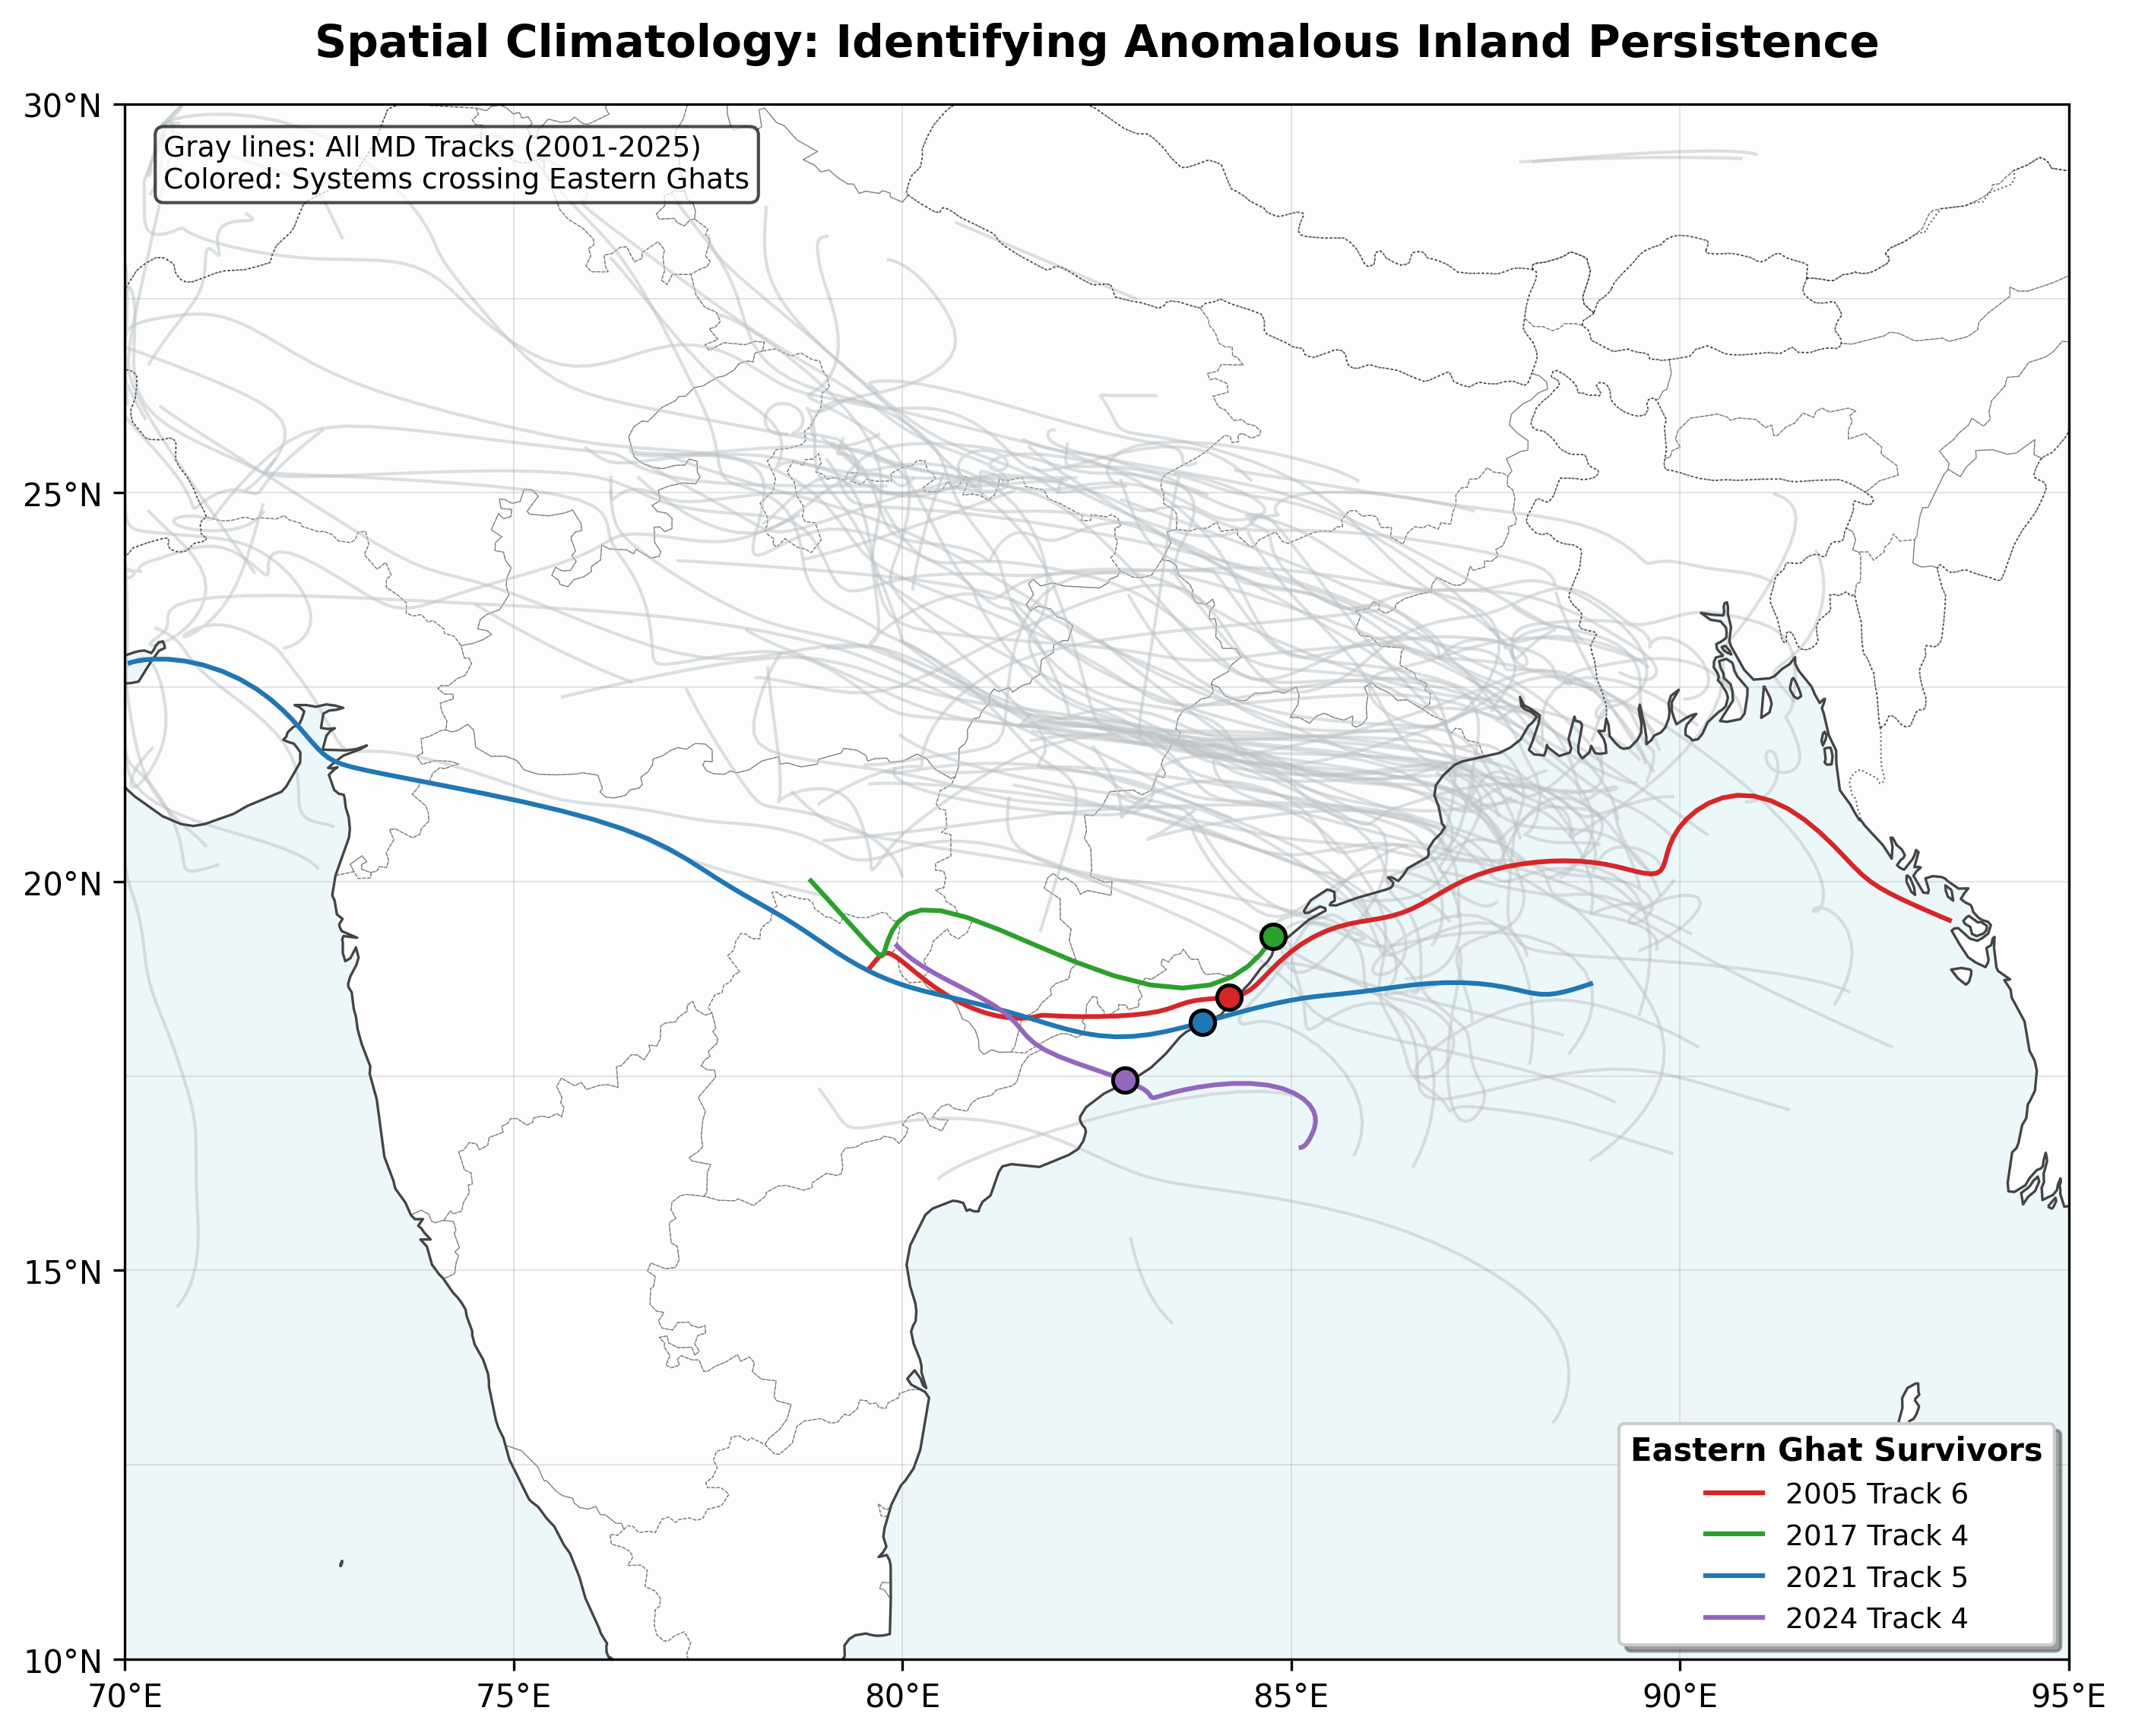
\includegraphics[width=0.95\textwidth]{ghats_survivors_map}
  \caption[Spatial distribution of Eastern Ghats
  survivors]{Comparison of standard MD tracks vs. the four anomalous
    survivor systems. Landfall points for survivors are marked with
    circles, indicating where the transition to Brown Ocean Effect
  thermodynamic maintenance begins.}
  \label{fig:ghats_survivors_map}
\end{figure}

The survival of these systems suggests that land-atmosphere coupling
(the BOE) provides sufficient energy to overcome the mechanical
frictional dissipation usually imposed by the Ghats.
 %% Results
%%  Chapter 5 - Discussion

\ifpdf
\graphicspath{{chapters/Figs/}{chapters/Figs/Raster/}{Figs/PDF/}{Figs/}}
\else
\graphicspath{{chapters/Figs/}{chapters/Figs/Vector/}{Figs/}}
\fi

\chapter{Discussion}
\label{ch:discussion}

\section{The BOE Mechanism in Indian Monsoon Depressions}
\label{sec:disc_boe}

The convergent lines of evidence assembled in
Chapter~\ref{ch:results} support a coherent mechanistic narrative.
Long-lived MDs maintain inner-core LHF at levels comparable to the
Bay of Bengal after landfall (Section~\ref{subsec:hovmoller_slhtf}),
their boundary layers remain near-saturated, and soil moisture
increases progressively beneath the inner core
(Section~\ref{subsec:hovmoller_swvl1}).

\subsection{LHF Magnitude and Cloud Cover Limitations}
The LHF magnitudes observed (70--120\,W\,m$^{-2}$) are lower than
extreme Atlantic BOE cases ($>200$\,W\,m$^{-2}$) reported by
\autocite{andersen2014insights}. This quantitative difference is
physically expected. In the Indian summer monsoon, persistent cloud
cover reduces solar insolation at the surface compared to the clearer
skies of the US Great Plains. However, because the Indian soil is
often near-saturated (ASMI $> 0.35$), the Bowen ratio remains
exceptionally low. This suggests that in the Indian context, the BOE
is driven by the \emph{efficiency} of moisture transfer rather than
high absolute energy input.

% \subsection{Soil Moisture Memory and ASMI Thresholds}
% Our finding that a 7-day ASMI lag better predicts persistence than
% a 14-day lag aligns with the soil moisture memory timescales of
% clay-loam soils common in the Odisha and Chhattisgarh basins. The
% threshold of 0.35\,m$^3$m$^{-3}$ identified in
% Section~\ref{subsec:asmi_results} serves as a "hydrological
% trigger" for the BOE, echoing the proxy findings of \autocite{kishtawal2013}.

\section{The Eastern Ghats as a Thermodynamic Filter}
\label{sec:disc_ghats}

As shown in Section~\ref{sec:results_elevation}, the Eastern Ghats do not
act as a binary wall. Instead, they function as a filter. Non-BOE
systems undergo structural collapse due to orographic moisture
stripping on the windward slopes. Conversely, BOE-active systems
exploit the high leeward soil moisture. The leeward speed recovery
observed in the composite analysis (Section~\ref{subsec:ts_speed}) is
a significant operational finding: it suggests that the land surface
can re-energize a system after terrain-induced disruption, provided
the land-atmosphere coupling is sufficiently strong.

% \chapter{Discussion}
% \label{ch:discussion}
%
% \section{The BOE Mechanism in Indian Monsoon Depressions}
% \label{sec:disc_boe}
%
% The convergent lines of evidence assembled in
% Chapter~\ref{ch:results} support a coherent mechanistic narrative.
% Long-lived MDs maintain inner-core LHF at oceanic levels after
% landfall (Section~\ref{subsec:hovmoller_lhf}), their boundary layers
% remain near-saturated throughout the land phase
% (Section~\ref{subsec:hovmoller_dpd}), soil moisture increases
% progressively beneath the inner core
% (Section~\ref{subsec:hovmoller_swvl1}), and the Bowen ratio stays low
% (Section~\ref{subsec:ts_bowen}), all consistent with the BOE
% mechanism. These signals are absent or rapidly collapsing in
% short-lived systems.
%
% The LHF magnitudes observed in the Indian MD context (70 -
% 120\,W\,m$^{-2}$ during the land phase) are lower than those reported
% for extreme Atlantic BOE cases ($>200$\,W\,m$^{-2}$;
% \citealt{andersen2014insights, wakefield2021}). This quantitative
% difference is physically expected. Atlantic BOE events typically
% occur in late summer (August - October) over the warm, irrigated, or
% recently flooded soils of the US South and Midwest, where soil
% surface temperatures can reach 30 - 35$^\circ$C. Indian MDs traverse
% soils that are cooler (owing to monsoon cloud shading reducing
% insolation) and where the available radiation for evapotranspiration
% is partly offset by the thick cloud layer. Nevertheless, the
% 70\,W\,m$^{-2}$ BOE threshold derived by \autocite{andersen2013} is
% shown here to be achievable and sustained in the Indian context,
% confirming that the BOE is not an exclusively Atlantic phenomenon but
% operates in the Indian monsoon environment under appropriate soil
% moisture conditions.
%
% \subsection{The Self-Wetting Feedback and Its Upper Bound}
% \label{subsec:disc_feedback}
%
% The co-evolution of \texttt{swvl1} and precipitation in
% Section~\ref{subsec:ts_sm_tp} reveals that the BOE is not simply a
% response to antecedent conditions but involves an active
% self-reinforcing process during the land phase. This has an important
% implication: even a system making landfall with moderately low ASMI
% ($\sim 0.28$ - $0.35$\,m$^3$\,m$^{-3}$) may approach BOE-sustaining
% soil moisture levels after 12-18\,h of its own heavy precipitation.
% The antecedent condition determines the \emph{initial} LHF level at
% landfall; whether a system can sustain LHF above the BOE threshold
% over the subsequent 18 hours is also determined by how rapidly the
% self-wetting feedback can drive \texttt{swvl1} to the energy-limited regime.
%
% This creates a practical implication for forecasting: a system making
% landfall over moderately moist soil may still qualify as a BOE
% candidate if its own initial precipitation is heavy enough to
% saturate the surface quickly. Conversely, an initially dry surface
% may prevent the self-wetting from occurring fast enough, even if
% large-scale atmospheric moisture advection is available.
%
% \subsection{Comparison with Prior Indian MD Studies}
% \label{subsec:disc_prior_india}
%
% The present study directly extends and observationally validates a
% sequence of prior works.
% \autocite{kishtawal2013enhancement} demonstrated, using proxy
% precipitation as an antecedent moisture indicator, that BOB
% depression inland penetration correlates with pre-storm soil wetness.
% This study replaces the proxy with direct ERA5 \texttt{swvl1}
% diagnostics and confirms the relationship over a 24-year climatology.
% The mechanistic link which \autocite{kishtawal2013enhancement} could not
% directly demonstrate from their proxy-based approach is established
% here through the Hovm\"{o}ller LHF signal and the Bowen ratio time series.
%
% \autocite{hunt2017effect} and \autocite{osuri2020} demonstrated through NWP
% sensitivity experiments that soil moisture initialisation affects MD
% simulation. The present observational evidence complements these
% modelling results by showing that the ERA5 soil moisture state
% without NWP forward integration is itself predictive of MD longevity,
% confirming that the signal is robustly present in the reanalysis record.
%
% \autocite{chang2009} identified land surface feedback as a modulator of
% post-landfall MD precipitation structure in WRF simulations. The
% Hovm\"{o}ller precipitation patterns in
% Section~\ref{subsec:hovmoller_tp} provide the observational
% equivalent: the sustained inner-core and contracted outer rainband
% structure after landfall in BOE-candidate systems mirrors precisely
% the model-simulated precipitation
% structure that \autocite{chang2009} attributed to land surface feedback.
%
% \autocite{ankur2022} showed that irrigated land cover enhances soil
% moisture and modulates MD behaviour. This study implicitly captures
% this effect through the ASMI (which integrates all moisture inputs,
% including irrigation) but cannot separate irrigation-driven soil
% moisture from monsoon-rainfall-driven soil moisture. This remains a
% limitation and an opportunity for future work
% (Section~\ref{sec:disc_limitations}).
%
% The BOE framework applied by \autocite{vijay2024boe} to the 1999 Odisha
% Super Cyclone demonstrated BOE-like inland maintenance of a
% post-landfall system in the Indian Ocean basin. The present
% climatological analysis shows that this mechanism is not confined to
% extreme events like the 1999 Super Cyclone but is a recurring process
% across the annual MD population.
%
% \section{The Role of the Eastern Ghats and Its Interaction with the BOE}
% \label{sec:disc_ghats}
%
% The differential translational speed recovery documented in
% Section~\ref{subsec:ts_speed}
% provides the most direct evidence for a BOE-terrain interaction. Both
% long-lived and short-lived systems decelerate over the Ghats, but
% only long-lived (BOE-candidate) systems recover speed on the leeward
% side. This differential is interpreted as follows.
%
% The BOE maintains the pressure gradient force of the MD vortex by
% sustaining deep convection on the leeward side through continuous LHF
% from the wet soil.
% In the absence of BOE, frictional decoupling during Ghats crossing
% increases vortex tilt and degrades the efficiency of the convective
% organisation.
% Without a local surface energy source to sustain convection on the
% leeward side, the vortex cannot recover its coherence and the system
% dissipates. With BOE, the leeward soil (which has been wetted by the
% windward-side precipitation that spilled over the terrain gaps)
% provides sufficient LHF to re-moisten the boundary layer, maintain
% CAPE, and re-organise convection around the re-emerging surface low.
%
% The windward-leeward DPD asymmetry (Section~\ref{subsec:ts_dpd_asymmetry})
% provides the boundary-layer moisture perspective on this process:
% BOE-candidate
% systems show smaller leeward DPD increase during terrain crossing, confirming
% that surface evapotranspiration is actively counteracting the
% orographic drying
% on the leeward side.
%
% \section{Surface Energy Partitioning and the Bowen Ratio}
% \label{sec:disc_bowen}
%
% The Bowen ratio trajectory (Section~\ref{subsec:ts_bowen}) is the
% most accessible single-variable summary of the post-landfall
% thermodynamic fate of an MD. The divergence between BOE-candidate and
% non-BOE systems is rapid and quantitatively large: a $\beta$
% difference of $\sim 0.6$-$0.8$ between the two populations after
% 24\,h of land transit represents a fundamentally different surface
% energy regime. The ERA5 HTESSEL land surface model represents this
% regime transition through its soil hydraulic parameterisation, and
% the consistency between the LHF, SHF, \texttt{swvl1}, and DPD time
% series provides confidence that the model is capturing the physically
% relevant transition correctly at the synoptic scale, even if the
% absolute magnitudes are uncertain (Section~\ref{sec:disc_limitations}).
%
% % \section{Implications for Operational Forecasting}
% % \label{sec:disc_forecasting}
% %
% % \yellownote{FIX: refrences}
% % The ASMI-duration relationship (Section~\ref{subsec:asmi_duration}) and the
% % BOE LHF threshold behaviour (Section~\ref{subsec:boe_identified}) together
% % suggest that a simple two-step operational indicator can be defined:
% %
% % \begin{enumerate}
% %   \item \textbf{Pre-landfall ASMI flag}: if the 7-day ASMI over the expected
% %     inland track corridor exceeds $0.35$\,m$^3$\,m$^{-3}$, issue an alert
% %     for possible anomalous inland persistence.
% %   \item \textbf{Post-landfall LHF monitoring}: if the ERA5T (near-real-time)
% %     inner-core LHF remains $\geq 70$\,W\,m$^{-2}$ for $\geq 12$\,h during
% %     the land phase, confirm BOE candidacy and revise the inland rainfall
% %     forecast accordingly.
% % \end{enumerate}
% %
% % This two-step procedure is consistent with the operational framework
% % advocated by \autocite{lodh2022improving}, who demonstrated that soil moisture
% % assimilation improves NWP post-landfall MD prediction, and
% \autocite{osuri2020},
% % who showed that correct soil moisture initialisation is a primary
% determinant
% % of MD simulation skill.
%
% % \section{Scope and Limitations}
% % \label{sec:intro_scope}
% %
% % ERA5 reanalysis (0.25$^\circ$, hourly) is the primary dataset; IMD
% % monsoon reports provide observational validation. The study covers
% % June-September for 2001-2025. At ERA5 spatial resolution ($\approx
% % 28$\,km), mesoscale inner-core convective structure is not
% % resolved, so results characterise synoptic-scale thermodynamic evolution.
%
% \section{Limitations and Sources of Uncertainty}
% \label{sec:disc_limitations}
%
% A systematic assessment of the uncertainties in this study is essential for
% correctly interpreting the magnitude and generality of the results.
%
% \subsection{ERA5 Soil Moisture Overestimation over India}
% \label{subsec:lim_swvl1_bias}
%
% The ERA5 land surface model (HTESSEL) has been shown to
% systematically \emph{overestimate} near-surface soil moisture
% (\texttt{swvl1}) over the Indian subcontinent during the monsoon
% season. \autocite{osuri2020} noted that ERA5 HTESSEL soil moisture over
% the Gangetic plains and Odisha tends to be biased high relative to
% in-situ measurements and SMAP satellite retrievals during
% July-August. The primary causes are:
% \begin{enumerate}
%   \item Overestimation of monsoon precipitation in ERA5
%     \autocite{hersbach2020era5}, which directly wets the soil;
%   \item Underestimation of drainage rates in the HTESSEL hydraulic
%     scheme over clay-loam soils; and
%   \item The absence of explicit irrigation in the model,
%     paradoxically leading to a different type of bias the model does
%     not represent irrigation-enhanced soil moisture but may partially
%     compensate through precipitation overestimation.
% \end{enumerate}
%
% \textbf{Implications for this study.} If \texttt{swvl1} is
% systematically overestimated by $\Delta\theta \approx
% 0.03$-$0.06$\,m$^3$\,m$^{-3}$ during July-August (consistent with the
% bias range reported by \citealt{osuri2020}), then the soil moisture threshold
% of $0.35$\,m$^3$\,m$^{-3}$ identified in this study as a predictor of
% BOE candidacy may be biased high by a similar amount. The \emph{true}
% physical threshold for BOE-enabling soil moisture may therefore be
% closer to $0.29$-$0.32$\,m$^3$\,m$^{-3}$ in terms of actual soil moisture.
% Similarly, the LHF values from ERA5 may be overestimated if the model
% is presenting unrealistically moist soils that evaporate at
% artificially high rates.
% The BOE LHF signal identified here should therefore be treated as an
% upper bound on the actual land-phase LHF, with the true signal
% potentially 10-20\,\% lower.
%
% \textbf{Mitigation.} The use of relative comparisons (BOE candidates
% vs non-BOE systems, ocean phase vs land phase) partially mitigates
% the impact of the absolute bias, as both populations are affected by
% the same systematic overestimation.
% The discrimination between long-lived and short-lived systems, and
% between BOE and non-BOE candidates, is based on differences in LHF
% and \texttt{swvl1} rather than their absolute values, making the
% classification methodology less sensitive to the bias than an
% approach that relies on absolute thresholds.
%
% \subsection{ERA5 Spatial Resolution and Inner-Core Representation}
% \label{subsec:lim_resolution}
%
% At $0.25^\circ$ ($\approx 28$\,km), ERA5 cannot resolve the
% mesoscale convective
% organisation of the MD inner core. The innermost radial bin of the
% Hovm\"{o}ller
% ($r < 25$\,km) contains at most one ERA5 grid point at any time step, and the
% values at this bin are single-point interpolations rather than
% spatial averages.
% Results for $r < 50$\,km should be interpreted as indicative of
% inner-core scale
% behaviour rather than as precise spatial measurements. In particular, the
% precipitation values in the inner-core bin may underestimate peak convective
% rainfall by a factor of 2-3 relative to the actual rainfall intensity at those
% scales, based on comparisons between ERA5 and GPM IMERG in the Indian monsoon
% context \autocite{hersbach2020era5}.
%
% \subsection{ERA5 Accumulated Flux De-Accumulation Errors}
% \label{subsec:lim_deaccum}
%
% The ERA5 LHF and SHF are provided as accumulated values in J\,m$^{-2}$, and
% instantaneous fluxes are derived by differencing consecutive
% accumulation steps
% (Equation~\ref{eq:deaccumulate}). This de-accumulation introduces noise at the
% hourly timescale because the assimilation system generates a new model run at
% each assimilation cycle (every 12\,h), and the accumulated flux is
% reset at the
% start of each run. Values in the first hour of each 12-h assimilation window
% may be affected by initialisation shock and should be treated with caution.
% This issue is most significant for the LHF values near the landfall
% transition,
% which may coincide with an assimilation cycle boundary.
%
% \subsection{SRTM Terrain Representation}
% \label{subsec:lim_srtm}
%
% The SRTM 1-arc-second DEM was acquired in February 2000 (northern winter) and
% represents a point-in-time surface elevation. While the Eastern Ghats bedrock
% elevation has not changed materially since 2000, the SRTM elevation model
% includes the canopy height of forests in the original data, which can add
% 10-20\,m to the ``terrain'' elevation in forested hill areas. For the bulk
% of the terrain analysis (identifying elevation zones of 200-1000\,m), this
% offset is negligible. However, for very precise calculations involving
% slope and roughness, the canopy contribution introduces sub-grid uncertainty
% in the 30-m DEM that is smoothed out when interpolated to track-point
% resolution.
%
% \subsection{Sample Size and Statistical Power}
% \label{subsec:lim_sample}
%
% \yellownote{TODO: update values}
% The 24-year record yields [N$_\text{total}$] confirmed MDs, of which
% [N$_\text{land}$] are land-falling and [N$_\text{BOE}$] qualify as
% BOE candidates. With a BOE-candidate sample of order 10-20 systems,
% the antecedent soil moisture duration correlation and
% Topographic-induced mechanical blocking duration correlation should
% be considered statistically suggestive rather than definitive:
% correlations significant at $p < 0.05$ but not at $p < 0.01$ could
% arise by chance with this sample size. Extension to the full ERA5
% back-extension record (1940-present) or cross-validation with MERRA-2
% would substantially increase statistical power.
%
% \subsection{Land Use, Irrigation, and HTESSEL Representativeness}
% \label{subsec:lim_landuse}
%
% ERA5 HTESSEL does not include explicit representation of agricultural
% irrigation, which is a major contributor to soil moisture over the
% Gangetic plains during the monsoon season \autocite{ankur2022}. In
% reality, irrigation may maintain \texttt{swvl1} at high levels even
% during break periods when natural monsoon rainfall is insufficient.
% The ASMI therefore underrepresents the contribution of irrigation to
% antecedent soil moisture in the most agriculturally active regions.
% Conversely, the absence of irrigation means that ERA5's
% \texttt{swvl1} may underestimate actual soil moisture in the Gangetic
% plains during break periods preceding MD landfall counteracting the
% overestimation bias discussed in Section~\ref{subsec:lim_swvl1_bias}
% and making the net bias direction uncertain in this specific context.
%
% \subsection{Shallow Soil Layer Representation}
% \label{subsec:lim_soil_depth}
%
% This study uses ERA5 \texttt{swvl1} (0-7\,cm), the uppermost soil
% layer, as the primary soil moisture variable. For the short-timescale
% (hourly) LHF diagnostics, \texttt{swvl1} is the most appropriate
% variable as it is most directly coupled to surface evaporation.
% However, for multi-day BOE events lasting $\geq 96$\,h, sustained
% evapotranspiration draws on deeper soil layers (\texttt{swvl2}:
% 7-28\,cm; \texttt{swvl3}: 28-100\,cm). The \texttt{swvl1} layer can
% be dried substantially by the first day of a BOE event's
% precipitation and LHF, even if the deeper layers remain moist enough
% to sustain root-zone evapotranspiration through capillary rise. The
% ASMI using only \texttt{swvl1} may therefore underestimate the total
% moisture reservoir available to sustain BOE in systems lasting $\geq 4$ days.
%
% \subsection{Scope of the Vortex Analysis}
% \label{subsec:lim_vortex}
%
% The three-dimensional dynamical structure of the MD warm/cold core
% evolution, pressure-level vorticity budgets, vertical tilt, IVT, and
% $\theta_e$ vertical profiles was not examined in this thesis. These
% quantities provide a complementary dynamical perspective on the BOE
% and terrain interaction that would strengthen the mechanistic
% attribution. The diagnostic tools for these analyses
% (\texttt{vortex\_analysis.py}) have been implemented and tested as
% part of the codebase but the results are deferred to future work.
%
% \subsection{Fixed Spatial Buffer and Track-Centre Uncertainty}
% \label{subsec:lim_buffer}
%
% The 100\,km spatial buffer used for track-following time series is a
% fixed parameter.
% The optimal buffer scale depends on the size of the MD circulation
% at any given
% time, which varies during the life cycle (contracting as the system decays).
% A fixed buffer may include grid points outside the vortex
% circulation during the
% peak land phase, diluting the inner-core flux signal with background values.
% Sensitivity tests with 50\,km and 200\,km buffers (not shown) reveal that the
% qualitative conclusions are robust, but the quantitative LHF values change by
% $\pm 15$\,\% depending on the buffer choice.
%
% Furthermore, the ERA5 850\,hPa vorticity maximum used to define the
% track centre
% may be displaced 25-75\,km from the actual low-level pressure minimum owing to
% the coarse model resolution and the complex multi-scale structure of the MD
% circulation. This positional uncertainty propagates directly into the
% Hovm\"{o}ller radial coordinate and the time-series buffer extraction.
%
% % \section{Mechanistic Role of Soil Moisture Memory}
% % \label{sec:disc_memory}
% %
% % The persistence of LHF is tied to the soil moisture memory, as
% % evidenced by the coupling efficiency metrics.
% %
% % \yellownote{TODO}
% % \begin{figure}[ht]
% %   \centering
% %   % \includegraphics[width=0.8\textwidth]{output_2024/Global_soil_memory/all_tracks_soil_memory.csv}
% %   % Create a bar or scatter plot from this CSV data
% %   \fbox{\rule{0pt}{7cm}\rule{0.82\textwidth}{0pt}}
% %   \caption{Soil moisture memory scales across the MD ensemble.}
% %   \label{fig:soil_memory}
% % \end{figure}
%
% \section{Historical Context and Prior Work on Indian MD Climatology}
% \label{sec:md_climatology}
%
% \subsection{Comparison of This Study with Prior Methodology}
% \label{subsec:methodology_comparison}
%
% Table~\ref{tab:prior_methods} summarises the methodological
% approaches of prior Indian MD soil moisture studies and positions the
% present study relative to them.
%
% \begin{table}[H]
%   \centering
%   \caption[Comparison of prior Indian MD soil moisture
%   studies]{Summary of prior Indian MD antecedent moisture and
%     post-landfall studies. ``Direct LHF'' indicates whether the study
%   measured surface latent heat flux directly rather than using a proxy.}
%   \label{tab:prior_methods}
%   \begin{tabular}{p{3cm}p{3cm}p{2.8cm}p{3.2cm}}
%     \toprule
%     \textbf{Study}                   & \textbf{Method}
%     & \textbf{Direct LHF?} & \textbf{Key Limitation} \\
%     \midrule
%     \autocite{kishtawal2013enhancement} & Antecedent rainfall proxy
%     & No                   & Proxy, fixed grid       \\
%     \autocite{chang2009}                & WRF NWP sensitivity
%     & No (model)           & Single event            \\
%     \autocite{hunt2017effect}           & NWP SM perturbation
%     & No (model)           & Model, not obs          \\
%     \autocite{osuri2020}                & NWP + ASCAT SM
%     & No (model)           & Model, not obs          \\
%     \autocite{vijay2024boe}             & ERA5 case study
%     & Partial              & Single event, 1999      \\
%     \textbf{This study}              & \textbf{Azimuthal
%     Hovm\"{o}ller + ERA5} & \textbf{Yes}  & ERA5 resolution limits \\
%     \bottomrule
%   \end{tabular}
% \end{table}
%
% The primary novelty of the present study-which
% Table~\ref{tab:prior_methods} makes explicit-is the combination of
% (i) \emph{direct} LHF measurement from ERA5 (not a proxy),
% (ii) a \emph{storm-centred} diagnostic (Azimuthal Hovm\"{o}ller) that
% removes the background climatological gradient, and
% (iii) a \emph{systematic} multi-year (2001-2025) climatology rather
% than single-event analysis.
%
% \subsection{Annual Frequency and Seasonal Distribution}
% \label{subsec:md_frequency}
%
% Historically, the Bay of Bengal generates approximately 5-7 Monsoon
% Depressions per JJAS season, with peak activity in July and August
% when the monsoon trough is at its most pronounced and BoB SSTs are at
% their seasonal maximum of 28-30$^\circ$C \autocite{sikka1977,
% rashid2005track}. The annual count is modulated by large-scale climate modes:
%
% \begin{itemize}
%   \item \textbf{ENSO:} El Ni\~no years typically suppress Indian
%     monsoon rainfall and reduce BoB LPS frequency, as the Walker
%     circulation weakens moisture flux over the BoB. La Ni\~na years
%     enhance LPS genesis.
%   \item \textbf{Indian Ocean Dipole (IOD):} Positive IOD (warm
%     western, cool eastern Indian Ocean) suppresses BoB moisture flux
%     and MD genesis; negative IOD enhances it.
%   \item \textbf{Madden-Julian Oscillation (MJO):} During the active
%     (convective) phase of the MJO over the Indian Ocean, background
%     moisture and vorticity over the BoB are enhanced, increasing MD
%     genesis probability.
% \end{itemize}
%
% \subsection{Landfall Statistics and Preferential Track Corridors}
% \label{subsec:md_landfall_stats}
%
% The majority of BoB MDs make landfall along the northern Andhra
% Pradesh-Odisha-West Bengal coastline, between approximately
% 82$^\circ$E and 88$^\circ$E longitude \autocite{rashid2005track}. This
% clustering reflects the combined effect of the monsoon trough axis
% (which directs systems toward northern Odisha) and the geometry of
% the BoB (which is wider in the south, giving systems forming farther
% south a longer ocean transit that brings them to the northern coast).
% Systems making landfall south of approximately 16$^\circ$N encounter
% the main Eastern Ghats range at higher topographic sensitivity, while
% systems making landfall north of 20$^\circ$N may partially circumvent
% the Ghats by tracking through the Mahanadi river-valley gap.
%
% % \yellownote{TODO: Discussions}
% % The Discussion on:
% % - Comparison of LHF values (70-120 W/m2) with BOE cases
% % (>200 W/m2) and physical explanation (monsoon cloud cover reduces
% % available radiation)
% % - Comparison of ASMI threshold (0.35 m3/m3) with Kishtawal (2013) proxy
% % - Explanation of why the 7-day lag outperforms the 14-day lag (soil
% % moisture memory timescale; clay loam retains moisture 3-7 days)
% % - Implications for operational forecasting
 %% Discussion
%%  Chapter 6 - Conclusions and Future Work
\chapter{Conclusions and Future Work}
\label{ch:conclusions}

\section{Principal Conclusions}
\label{sec:conclusions_main}

This thesis investigated the physical mechanisms allowing specific
Indian Monsoon Depressions (MDs) to persist for extended durations
and penetrate deep inland following landfall. Using hourly ERA5
reanalysis data over the 2001-2025 period and a MD-centered
diagnostic framework, the following principal conclusions are reached:

\begin{enumerate}
  \item \textbf{The Brown Ocean Effect (BOE) discriminates long-lived
    from short-lived systems.}
    Out of the \textbf{128} confirmed land-falling MDs identified,
    \textbf{38} systems(\textbf{29.7}\,\%) meet the established
    BOE criterion of inland Latent Heat Flux (LHF) $\geq
    70$\,W\,m$^{-2}$ sustained for $\geq 18$ consecutive hours.
    Importantly \emph{all} 38 BOE-candidate systems are long-lived
    ($\geq 96$\,h, with a mean duration of \textbf{138.3}\,h), while
    \emph{no} short-lived system qualifies under this thermodynamic
    threshold. This exclusive overlap demonstrates that the BOE is a
    necessary condition for anomalous inland persistence in the
    Indian monsoon environment.
  \item \textbf{The Azimuthal Hovm\"{o}ller framework captures the
    transition to a land-based energy source.}
    Long-lived MDs exhibit a distinct Hovm\"{o}ller signature
    characterized by an inward contraction of the precipitation
    signal. While initial landfall is dominated by outer-annular
    (100-250\,km) moisture advection, persisting systems shift to an
    inner-core ($<100$\,km) flux-dominated pattern. This signature,
    accompanied by sustained inner-core LHF and near-saturated
    boundary layer conditions (Dew Point Depression $<3$\,K),
    confirms that the system has successfully transitioned from
    relying on oceanic moisture to relying on local surface evapotranspiration.
  \item \textbf{The Eastern Ghats act as a thermodynamic filter
    rather than an absolute barrier.}
    Both long-lived and short-lived systems experience deceleration
    during terrain traversal, but they display fundamentally
    different leeward behavior. BOE-active systems exhibit
    translational speed recovery on the leeward side of the Ghats,
    indicating that sustained surface LHF from wet leeward soil
    maintains the pressure gradient force and vortex coherence. In
    contrast, non-BOE systems continue to decelerate and decay
    leeward of the terrain. Furthermore, systems aligned with major
    river-valley gaps (such as the Mahanadi corridor) show enhanced
    penetration, suggesting these gaps preserve critical low-level
    moisture inflow channels.
  \item \textbf{A self-wetting feedback loop maintains the inland
    depression core.}
    The co-evolution of surface variables and precipitation in
    track-following diagnostics demonstrates an active positive
    feedback loop: MD rainfall increases soil moisture, which in turn
    sustains latent heat release above the 70\,W\,m$^{-2}$ threshold.
    This mechanism allows the atmosphere to maintain oceanic-like
    convective organization over land, effectively masking the
    transition from sea to soil and allowing the depression to
    penetrate deep into the Indian landmass.
\end{enumerate}

\section{Potential for Future Operational Applications}
\label{sec:conclusions_operational}

The Azimuthal Hovmöller framework applied in this study offers a
novel MD-centered diagnostic capability for distinguishing BOE-active
from BOE-inactive systems. Real-time or near-real-time application of
this framework using ERA5T data or regional NWP model output could provide
extended guidance for post-landfall evolution, complementing conventional
decay prediction. The strong Hovmöller signals - inner-core LHF
maintenance, soil moisture progressive wetting, DPD near-saturation,
and precipitation inward contraction - provide a multi-variable
signature of the BOE mechanism. Operational meteorological centres
with access to reanalysis or NWP-derived fluxes can apply similar diagnostics at
landfall time to assess whether a system exhibits BOE signatures and
adjust inland persistence guidance accordingly.

\section{Directions for Future Research}
\label{sec:conclusions_future}

\begin{enumerate}
  \item \textbf{Vortex-scale three-dimensional diagnostics.}
    Pressure-level analyses of warm/cold-core evolution, vorticity
    column coherence, Integrated Vapor Transport (IVT), and vortex tilt
    would provide a dynamical counterpart to the surface thermodynamic evidence,
    completing the mechanistic picture of the BOE in three dimensions.
  \item \textbf{Multi-reanalysis cross-validation.} Repeating the
    Hovm\"{o}ller analysis with MERRA-2 and JRA-55 would
    assess the sensitivity of the BOE signal to differences in land
    surface parameterisation (HTESSEL vs CLSM vs the JMA scheme) and
    quantify reanalysis uncertainty in the LHF and soil moisture
    signals by using soil type data.
  \item \textbf{Eastern Ghats gap-passage analysis.} A systematic
    comparison of landfall longitudes relative to the Godavari,
    Mahanadi, and Brahmani river-valley gaps would test whether
    gap-aligned landfalls correlate with longer inland persistence by
    preserving low-level moisture inflow channels through the terrain.
  \item \textbf{NWP sensitivity experiments.} Targeted WRF or Unified
    Model experiments with perturbed soil moisture initialisation for
    the specific BOE-candidate events identified in this observational
    analysis would provide a controlled modelling counterpart,
    isolating the causal role of the surface moisture state
    \autocite{hunt2017effect, osuri2020}.
    % \item \textbf{CMIP6 climate change projections.} Applying the
    %   Hovm\"{o}ller framework to CMIP6 historical and future scenario
    %   outputs would assess whether projected changes in monsoon
    %   rainfall, soil moisture, and temperature are likely to intensify or
    %   weaken the BOE contribution to MD inland persistence under
    %   late-21st-century conditions.
\end{enumerate}

\section{Closing Remarks}
\label{sec:conclusions_closing}

This thesis began with a meteorological question: "why do some landfalling
Monsoon Depressions persist for nearly a week while classical theory predicts
they should decay within days". The answer is that under sufficiently
moist land-surface conditions, the Indian land surface can
functionally mimic an ocean-not metaphorically, but physically,
called Brown Ocean. When the Gangetic plains have been pre-wetted by
weeks of prior monsoon rainfall, and when a Monsoon Depression drives
its own precipitation into already-saturated soils, the land surface
supplies latent heat at rates comparable to the warm Bay of Bengal it
just left. The atmosphere, unable to distinguish ocean from land,
maintains its convective organisation and sustained rainfall.

The Brown Ocean Effect is, in this sense, an emergent property of two
coupled systems: the Indian monsoon, which pre-conditions the land surface
over June-July through accumulated rainfall, and the Monsoon Depression,
which then exploits that pre-conditioned surface to extend its own lifetime.
The Eastern Ghats-which hundreds of kilometres of elevated terrain could be
expected to truncate depression tracks-are reduced to a moderate obstacle
that cannot stop the BOE when it is active. The terrain acts as a \emph{filter},
not a wall.

Monsoon Depressions are simultaneously among the most beneficial and
most hazardous of India's weather systems. They deliver critical
seasonal rainfall to water-stressed agricultural regions while also
triggering catastrophic multi-day flooding. The key insight of this
thesis is that post-landfall longevity is fundamentally determined by
the BOE mechanism and the antecedent soil moisture conditions that
enable it. This provides new understanding of this predictability problem.
As the Indian subcontinent continues to develop, as monsoon patterns
shift under climate change, and as agricultural irrigation
intensifies, the favorable conditions for the BOE may intensify or
diminish. The answer will determine whether India's most significant
inland weather systems become more or less predictable and more or
less dangerous-in the decades ahead.
 %% Conclusions and Future Work

% \chapter{Design Principles} \label{ch:Design}

It is not like I stated the \emph{Principles} at the beginning and then tried to follow them.
They emerged more naturally.
So the causal structure is more like
\[
    \raisebox{-0.15ex}{\parbox[c]{6em}{\centering made some design choices}}
    \mspace{12mu} \text{and} \mspace{10mu}
    \parbox[c]{7em}{\centering implemented certain features}
    \quad\longleadsto{}\quad
    \parbox[c]{10em}{\centering recognized \\\textcolor{gray}{at first subconscious} overarching principles}~.
\]
Anyway, here they are.
\begin{definition}[Design Principles] \label{def:Design Principles}
    The main design \emph{Principles} are:
    \begin{itemize}
        \item \textbf{Elegance} --- Aim for a classy, typographically elegant layout.
        \item \textbf{Structure} --- Create a smart, easy-to-reference, and skimmable structure.
        \item \textbf{Clarity} --- Eliminate distractions and strive for clear explanations. \qedhere
    \end{itemize}
\end{definition}
\begin{remark}[Common Goal, Alternative Definition via Antiprinciples]
    There is also an alternative point of view.
    The common goal of \Nref*{def:Design Principles} is to minimize the following \emph{Antiprinciples}:
    \begin{itemize}
        \item We should be concise, and that means fewer pages, the better.
              Long blocks of text without noticeable space between paragraphs are preferred (the reader should go on a walk to have some breathing spacetime).
        \item Avoid creating distinct anchor points for important concepts, since an attentive reader should be able to extract them from blocks of text.
        \item Do not waste time referencing earlier discussions and reflecting on them from the current context and point of view, as the reader is anyway making such connections all the time. \qedhere
    \end{itemize}
\end{remark}

Each of these principles is somehow reflected in the design choices and features included (or omitted) in \TeXsis{}, see \Cref{ch:Features} for more details.

\begin{remark}[Disclaimer]
    The following is at places highly opinionated, and not applicable to all scenarios and use-cases.
    I tried to describe my reasons for specific design choices, with which you can certainly disagree.
    I hope that at least it can provoke more people \emph{(especially you!)} to contemplate about document creation, ideally resulting in production of documents with overall better quality.
\end{remark}

% \chapter{Usage of \TeXsis{}} \label{ch:Usage}

To quickly familiarize yourself with the \TeXsis{} template, we will go through the basic structure of the template files and explain how to use them.
First, take a look at \Cref{fig:file-structure} for a visual representation of the file structure.
% \begin{figure}[!ht]
%     \fcapside[\FBwidth]{%
%         \captionsetup{parskip = .5\baselineskip plus 1pt}%
%         \caption[\TeXsis{} Template File Structure]{%
%             \TeXsis{} template file structure.
%
%             The main file is \path{thesis.tex}.
%             % FIX:
%             % It does not contain the actual content of the document, but instead \fakemacro{\include}s the chapters and \emph{front matter} pages from the corresponding directories.
%             It does not contain the actual content of the document, but instead \texttt{\textbackslash include}s the chapters and \emph{front matter} pages from the corresponding directories.
%
%             Make sure to fill all PDF \grayenclose{meta}data --- like title, author, etc.~--- in the \path{preamble/data.tex} file.
%             The bibliography/reference data is stored in the \path{preamble/bibliography.bib} file.
%
%             % FIX:
%             % All of the \TeXsis{} tweaks and settings located in files under \path{preamble/...} directories are loaded by the \path{preamble/main.tex} file, which is itself \fakemacro{\input}ed in the \path{thesis.tex} file.
%             All of the \TeXsis{} tweaks and settings located in files under \path{preamble/...} directories are loaded by the \path{preamble/main.tex} file, which is itself  \texttt{\textbackslash \input}ed in the \path{thesis.tex} file.
%
%             The \path{.latexmkrc} file contains a configuration for the \textsf{latexmk} tool, which provides a convenient way to compile the document.
%         }%
%         \label{fig:file-structure}%
%     }{%
%         \begin{tikzpicture}[dirtree]
%             \node[directory] {\TeXsis{} Root Directory/}
%             child { node {thesis.tex}}
%             child { node {LICENSE}}
%             child { node {README.md}}
%             child { node[directory] {chapters/...}}
%             child { node[directory] {figures/...}}
%             child { node[directory] {frontmatter/...}}
%             child { node[directory] {preamble/}
%                 child { node {bibliography.bib}}
%                 child { node {data.tex}}
%                 child { node {main.tex}}
%                 child { node[directory] {...} }
%             }
%             child [missing] {} child [missing] {} child [missing] {} child [missing] {}
%             child { node {.latexmkrc}}
%             child { node {.gitignore}}
%             child { node {.gitattributes}}
%             child { node[directory] {.github/...}}
%             ;
%         \end{tikzpicture}%
%     }
% \end{figure}

The usual workflow looks something like this:
\begin{itemize}
    \item \textsf{Metadata.} Fill in the \path{preamble/data.tex} file with the necessary information about the document --- title, author, and other \emph{metadata}.
    \item \textsf{Content.} Write the content of the document in the \path{chapters/} directory.
          If you need more chapters, just create a new file, and \macro{\include} it in the \path{thesis.tex} file at appropriate place.
    \item \textsf{Figures.} To include figures, you can put them in the \path{figures/} directory.
          Since this directory is by default included in \macro{\graphicspath}, there is no need to specify full/relative path, and it is enough to use just the filename in the \macro{\includegraphics} command.
    \item \textsf{Citations.} Using \grayenclose{for example} \macro{\autocite} macro, you can cite in the text any entry added to the \path{preamble/bibliography.bib} file.
\end{itemize}

\begin{remark}[Toggles]
    There are a couple of \emph{toggles} in the \path{thesis.tex} file that can be used to customize style/layout/creation of the document:
    \begin{itemize}
        \item \textsf{Page Layout} --- you can choose between \emph{Single-Side} or \emph{Two-Sided} printing by uncommenting the appropriate \macro{\documentclass} line.
        \item \textsf{Fancy Style} \textcolor{gray}{(default:\,\texttt{enabled})} --- if the default style is not to your liking, you can disable some of the more \enquote{fancy} stylistic elements by using the \custommacro{\FANCYfalse} line.
        \item \textsf{Work-In-Progress Version} \textcolor{gray}{(default:\,\texttt{disabled})} --- if you want to mark the document as a \emph{Draft}, leave the \custommacro{\WIPtrue} line uncommented (comment out for the final version).
              \begin{itemize}
                  \item \textsf{Extra Margin} \textcolor{gray}{(default:\,\texttt{disabled})} --- the \emph{Draft} document will include extra right margin (for notes and corrections) when you enable it using \custommacro{\EXTRAMARGINtrue}.
              \end{itemize}
        \item \textsf{Link Boxes} \textcolor{gray}{(default:\,\texttt{enabled})} --- drawing of link/reference boxes can be disabled by \custommacro{\LINKBOXESfalse} command (improves compilation time).
        \item \textsf{Censored Version} \textcolor{gray}{(default:\,\texttt{disabled})} --- if you want to censor chosen parts of the document, include the \custommacro{\CENSORtrue} line.
        \item \textsf{Include Only \ldots{}} --- if you want to compile only a subset of chapters, you can utilize the \custommacro{\includeonlysmart} command. \qedhere*
    \end{itemize}
\end{remark}

\begin{remark}[MFF CUNI Template Compatibility]
    \TeXsis{} can be used out of the box for theses at the Faculty of Mathematics and Physics, Charles University in Prague.
    Just be sure to include all \emph{front matter} pages and fill out necessary data:
    \begin{itemize}
        \item \textsf{Title Page} with the faculty logo (among other things),
        \item \textsf{Declaration},
        \item \textsf{Dedication} (optional),
        \item \textsf{Information Page} including the \textsf{Abstract}.
    \end{itemize}
    This is done by uncommenting the relevant lines in the main \path{thesis.tex} file.

    Layout of these front matter pages is adapted and modified from the original MFF CUNI template \autocite{MaresTemplate}.
    However, always make sure it is compliant with the faculty guidelines, otherwise please raise an issue on \textsf{GitHub} \autocite{TeXsis}.
\end{remark}

\begin{remark}[License]
    If you want to make your document publicly available (together with the source code), you should not forget to include an appropriate license of your choice --- change the \path{LICENSE} file, specifying the \href{https://creativecommons.org/publicdomain/zero/1.0/}{\texttt{CC0 1.0 Universal}} license of \TeXsis{}.
\end{remark}

% \chapter{Features of \TeXsis{}} \label{ch:Features}

In the following sections, we will describe the features of \TeXsis{} template, implemented by utilizing various \LaTeX{} packages and custom macros.

\begin{remark}[Packages and Macros]
    We will refer to various \LaTeX{} packages and macros using the following styles:
    \begin{itemize}
        \item \package{package} --- a package (together with a link to its \textsf{CTAN} page),
        \item \macro{\macro} --- a command/macro, either built-in or provided by a package,
        \item \custommacro{\custommacro} --- a custom macro defined in the \TeXsis{} template. \qedhere*
    \end{itemize}
\end{remark}

\section{Code Organization}%
\label{sec:Code Organization}

To avoid large and hard to navigate preamble files, the code is organized into multiple directories/files in the \path{preamble/} directory, each focusing on a particular function/feature, see \Cref{fig:preamble-file-structure}.
% \begin{figure}[!ht]
%     \fcapside[\FBwidth]{%
%         \captionsetup{parskip = .5\baselineskip plus 1pt}%
%         \caption[Structure of Preamble Directory]{%
%             Structure of the \path{preamble/} directory.
%
%             It is critical that the \path{preamble/pdfA-compliance/glyphtounicode.tex} file ensuring the PDF/A compliance is sourced before \fakemacro{\documentclass}.
%
%             The \path{preamble/toggles.tex} files defines various toggles, which should be appropriately set right after.
%             Finally, the rest of \grayenclose{preamble} files are then loaded through the \path{preamble/main.tex} file.
%
%             When possible, add your own tweaks and macros to the \path{preamble/user/} directory reserved for this purpose.
%             This way, you can easily update to newer versions of \TeXsis{} (hopefully) without conflicts.
%         }%
%         \label{fig:preamble-file-structure}%
%     }{%
%         \begin{tikzpicture}[dirtree]
%             \node[directory] {preamble/}
%             child { node {bibliography.bib}}
%             child { node {data.tex}}
%             child { node {toggles.tex}}
%             child { node {main.tex}}
%             child { node[directory] {debug/...}
%                 % child { node {commands.tex}}
%                 % child { node {line-numbers.tex}}
%             }
%             % child [missing] {} child [missing] {}
%             child { node[directory] {environments/...}
%                 % child { node {init.tex}}
%                 % child { node {remark-like.tex}}
%                 % child { node {theorem-like.tex}}
%                 % child { node {todo-like.tex}}
%             }
%             % child [missing] {} child [missing] {} child [missing] {} child [missing] {}
%             child { node[directory] {general/...}
%                 % child { node {colors.tex}}
%                 % child { node {floats.tex}}
%                 % child { node {hyperref.tex}}
%                 % child { node {typesetting.tex}}
%             }
%             % child [missing] {} child [missing] {} child [missing] {} child [missing] {}
%             child { node[directory] {hacks/...}
%                 % child { node {custom-reference-boxes.tex}}
%                 % child { node {fix-qed.tex}}
%                 % child { node {floatrow-parskip.tex}}
%             }
%             % child [missing] {} child [missing] {}
%             child { node[directory] {layout/...}
%                 % child { node {geometry.tex}}
%                 % child { node {headers.tex}}
%                 % child { node {numbering.tex}}
%                 % child { node {titles.tex}}
%                 % child { node {toc.tex}}
%             }
%             % child [missing] {} child [missing] {} child [missing] {} child [missing] {} child [missing] {}
%             child { node[directory] {math/...}
%                 % child { node {fonts.tex}}
%                 % child { node {macros.tex}}
%                 % child { node {packages.tex}}
%                 % child { node {spacing.tex}}
%             }
%             % child [missing] {} child [missing] {} child [missing] {} child [missing] {}
%             child { node[directory] {misc/...}
%                 % child { node {inkscape.tex}}
%                 % child { node {macros.tex}}
%                 % child { node {tikz.tex}}
%             }
%             % child [missing] {} child [missing] {} child [missing] {}
%             child { node[directory] {pdfA-compliance/...}
%                 % child { node {glyphtounicode.tex}}
%                 % child { node[directory] {LaTeX-find-glyph-name/}
%                 %     child { node {LaTeX-find-glyph-name.tex}}
%                 % }
%             }
%             % child [missing] {} child [missing] {} child [missing] {}
%             child { node[directory] {references/...}
%                 % child { node {backref.tex}}
%                 % child { node {biblatex-extra-fields.dbx}}
%                 % child { node {biblatex.tex}}
%                 % child { node {cite.tex}}
%                 % child { node {doi-eprint-url.tex}}
%                 % child { node {fields.tex}}
%                 % child { node {style.tex}}
%             }
%             % child [missing] {} child [missing] {} child [missing] {} child [missing] {} child [missing] {} child [missing] {} child [missing] {}
%             child { node[directory] {user/...}
%                 % child { node {macros.tex}}
%                 % child { node {math.tex}}
%             }
%             % child [missing] {} child [missing] {}
%             ;
%         \end{tikzpicture}%
%     }
% \end{figure}

\begin{remark}[Pointers to Directories/Files]
    If you want to tweak some aspect of the template --- or learn how a given feature is implemented --- pointers to the relevant directories/files are provided next to the subsequent section/subsection titles to help you navigate the code.
\end{remark}

\begin{remark}[Custom User Macros]
    Store your own macros in the \path{preamble/user/} directory, which is reserved precisely for this purpose.
    Then, if you would like to update to a newer version of \TeXsis{}, you will be having easier time --- less mixing of your code with the template code will result in fewer conflicts you must resolve manually.
\end{remark}

\begin{remark}[Auxiliary Files]
    To avoid cluttering the directories with \emph{auxiliary files} generated during the compilation, it is recommended to use the \macro{aux_dir} setting in the \path{.latexmkrc} file (enabled by default, the \macro{aux_dir} being \path{.aux/}).
    All auxiliary files are then stored in a separate directory, leaving the rest tidy.
\end{remark}

\begin{remark}[Suggestion: One Sentence Per Line]
    It is a good practice to follow \enquote{one sentence per line} rule (or something similar), since it improves diffs for versioning systems like \texttt{git}.
    Tools like \texttt{latexindent} can help.
    \begin{Note}
        My config for \texttt{latexindent} mostly works, but some corner cases can surface.
        Will share someday.
    \end{Note}
    If multiple sentences are on the same line, changing just one word results in the whole line being marked as changed, making it harder to see how much the text was actually changed in a given commit.
\end{remark}



\section{Page Layout and Style}%
\label{sec:Page Layout}
\dirTeXsis{preamble/layout/}

We will first describe the page layout and style, which includes page dimensions, headers and footers, page numbering, and heading style.

\subsection{Page Dimensions, Printing Layout}%
\label{sub:Page Dimensions}
\fileTeXsis{preamble/layout/geometry.tex}

Using \package{geometry} package --- set up the page layout (supported single/double-sided printing).
Apply \macro{\flushbottom} --- try to make text body on all pages have the same height.

\subsection{Page Headers and Footers}%
\label{sub:Headers Footers}
\fileTeXsis{preamble/layout/headers.tex}

Using \package{fancyhdr} package --- page headers and footers --- consistent style also for initial page of a chapter (not totally different style with numbering in the bottom center \ldots).

\subsection{Page Numbering}%
\label{sub:Page Numbering}
\fileTeXsis{preamble/layout/numbering.tex}

Placing custom \custommacro{\frontmatter}, \custommacro{\mainmatter}, and \custommacro{\backmatter} macros at appropriate places in \path{thesis.tex}, \emph{Roman numbering} is set up for \emph{front matter}, that is until the start of first numbered chapter, and then \emph{Arabic numbering} for the rest of the document.


\subsection{Heading Style}%
\label{sub:Heading Style}
\fileTeXsis{preamble/layout/titles.tex}

Pretty chapter heading style --- big calligraphic number/letter behind the title.


\section{Sane Typographical Defaults}%
\label{sec:Sane Typographical Defaults}
\dirTeXsis{preamble/general/}

Now we will concern ourselves with more intricate and detailed typography, more at level of paragraphs, sentences, words, and even letters.

\subsection{Paragraphs}%
\label{sub:Paragraphs}
\fileTeXsis{preamble/general/typesetting.tex}

No paragraph indentation, proper space between paragraphs --- \package{parskip}.

\subsection{Floats, Captions}%
\label{sub:Floats_Captions}
\fileTeXsis{preamble/general/floats.tex}

Caption styling includes a slight hang, \macro{\footnotesize} font, and a bold sans label.
See \Cref{appendix:example} for a showcase of the different caption types.


\subsection{Font and Related Stuff}%
\label{sub:Font}
\fileTeXsis{preamble/general/typesetting.tex}

The default choice are \emph{Latin Modern} fonts --- a classic really.
Various families and shapes are typically used for different purposes:
\begin{itemize}
    \item \emph{Serif} family for the main text
    \item \emph{Slanted} shape for emphasis using \macro{\emph} macro (instead of the default \emph{Italic} shape, which is reserved mainly for math formulas)
          \begin{remark}[Nested Emphasis]
              Nested emphasis is displayed in \emph{Italic} shape.
              It is rather rare to nest an \emph{additional \emph{emphasis} inside an emphasis}.
          \end{remark}
    \item \emph{(Bold) Sans} family for headings and other structural elements
    \item \emph{Typewriter} family for computer code and similar stuff
\end{itemize}
\vspace{1ex}

\begin{example}
    Quick showcase of some font families and shapes:\par \leftskip=1em

    {                  This is Latin Modern Serif \(\alpha = 2^{2}\)}\\
    {\slshape          This is Latin Modern Serif Oblique \(\alpha = 2^{2}\)}\\
    {\bfseries         This is Latin Modern Serif Bold \(\alpha = 2^{\bm{{2}}}\)}\\
    {\bfseries\slshape This is Latin Modern Serif Bold Oblique \(\alpha = 2^{2}\)}

    {\sffamily                  This is Latin Modern Sans \(\alpha = 2^{2}\)}\\
    {\sffamily\slshape          This is Latin Modern Sans Oblique \(\alpha = 2^{2}\)}\\
    {\sffamily\bfseries         This is Latin Modern Sans Bold \(\alpha = 2^{2}\)}\\
    {\sffamily\bfseries\slshape This is Latin Modern Sans Bold Oblique \(\alpha = 2^{2}\)}
\end{example}
\begin{Note}
    Sans math font has problems with showing properly all bold symbols (sub/superscripts don't work automatically).
\end{Note}

For consistent quotation use \macro{\enquote} macro provided by \package{csquotes}.

\subsection{\texorpdfstring{Micro-\!Typography}{Micro-Typography}}%
\label{sub:Micro-Typography}
\fileTeXsis{preamble/general/typesetting.tex}

Enable micro-typographic extensions with package \package{microtype}, most prominently character protrusion and font expansion.

Following quote from \package{microtype} documentation nicely explains what it is about:
\begin{displayquote}
    Micro-typography is the art of enhancing the appearance and readability of a document while exhibiting a minimum degree of visual obtrusion.
    It is concerned with what happens between or at the margins of characters, words or lines.
    Whereas the macro-typographical aspects of a document (i.e., its layout) are clearly visible even to the untrained eye, micro-typographical refinements should ideally not even be recognizable.
    That is, you may think that a document looks beautiful, but you might not be able to tell exactly why: good micro-typographic practice tries to reduce all potential irritations that might disturb a reader.
\end{displayquote}


\section{Document Structure}%
\label{sec:Document Structure}

It is important to have a clear and consistent structure of the document.
This can be achieved by using various environments for different types of content, and by providing clear and informative titles for each part of the document, thus making it easier to navigate and understand.

\subsection{Structure Environments}%
\label{sub:Structure Environments}
\fileTeXsis{preamble/environments/*.tex}
% \fileTeXsis{preamble/environments/init.tex}
% \fileTeXsis{preamble/environments/theorem-like.tex}
% \fileTeXsis{preamble/environments/remark-like.tex}
% \fileTeXsis{preamble/environments/todo-like.tex}

Inspired by the structured mathematical texts, enclosing various parts of the document in the corresponding environments can help to make the document more structured and easier to read.
Implemented mostly \package{tcolorbox} package and \package{keytheorems} (modern key--value interface for \package{amsthm}).

\begin{remark}[Default Environments]
    There are predefined boxed \enquote{theorem-like} environments for \textsf{Definition}, \textsf{Theorem}, \textsf{Lemma}, \textsf{Corollary}, \textsf{Proposition}, and non-boxed \enquote{remark-like} environments for \textsf{Remark}, \textsf{Proof}, \textsf{Example}, \textsf{Derivation}, \textsf{Calculation}, \textsf{Idea}, and \textsf{Tip} (these have at least a mark indicating the end of the environment).

    Names of the corresponding environments are lowercase, for example \texttt{definition}, \texttt{remark}, and so on.
    They also accept an optional argument for a short description.
\end{remark}

Some additional points about the \emph{structure environments}:
\begin{itemize}
    \item provide clear structure, enables high level of interlinking
    \item they make the text easy to skim through, quickly get an idea, and know roughly what to expect
    \item have shared numbering, together with tables, figures, equations --- leads to a linear increase of the reference number, making them easier to locate
    \item not only for physics/math texts, can be generally used to highlight key ideas
          % \begin{tip}[Custom Structure Environments]
          %     You can easily create additional \enquote{structure} environments, see \Cref{sec:Structure}.
          % \end{tip}
    \item avoid using emphasis for the whole body of \enquote{theorem-like} environments, since we already have a whole box around it to make them stand out
\end{itemize}
\vspace{1ex}

\begin{remark}
    There are also helper environments for \textsf{Todo}-like notes.
    By default, there are \textsf{Todo}, \textsf{Note}, \textsf{Suggestion}, and \textsf{Question} environments, but you can easily create your own.

    To avoid conflicts with possible existing macros/environments, names of these environments are capitalized, for example \texttt{Todo}, \texttt{Note}, and so on.
\end{remark}

\begin{Note}
    No \enquote{code listing} setup yet.
    PRs welcome.
\end{Note}

\subsection{References and Links}%
\label{sub:References Links}
\fileTeXsis{preamble/hacks/custom-reference-boxes.tex}

Custom reference/link/citation styles using \package{tcolorbox} package.
\begin{Note}[Slight Inconvenience --- Line Breaks]
    There is a slight inconvenience due to small flexibility around line breaks.
    It would be nice to have a proper workaround.
\end{Note}
\begin{remark}[Rationale]
    I like to have clearly distinguished references, links, and citations.
    By default, \package{hyperref} provides frames around links, but they are not that pretty, and the PDF viewer must support them.
    Using just colors can sometimes look better, but I still wasn't satisfied.

    Sometimes it is nice to know the precise location of the reference, especially when the document is printed and you cannot simply click on them.
    Therefore, the page number is (by default) included with \custommacro{\Cref}, see \Cref{rem:zref-clever}.
    Use the starred variant \custommacro{\Cref*} to omit it.
\end{remark}
\begin{remark}[Automatic Reference Type Detection] \label{rem:zref-clever}
    Package \package{zref-clever} provides \macro{\zcref} command --- similarly to the older, no longer maintained, \package{cleveref} package --- which automatically detects the type of reference, and formats it accordingly.
    This behavior is adapted in \TeXsis{} with the macro \custommacro{\Cref}, which wraps the link in nice box, and also shows a corresponding page number of the target.

    If you want the link to show the reference title, use \custommacro{\Nref} --- or the starred variant \custommacro{\Nref*} to omit the page number --- which utilizes \package{zref-titleref}.
\end{remark}

\subsection{Table of Contents and Outline/Index}%
\label{sub:Table of Contents and Index}
% \fileTeXsis{preamble/layout/toc.tex}

Clear and elegant Table of Contents, which includes all the important parts --- also \grayenclose{unnumbered} subsections, but in a more compact style.

Similarly, automatically populate the PDF Outline/Index (digital Table of Contents in PDF viewer).
It is very handy for navigating longer documents, and includes also other important pages other than just initial pages of main chapters: Title Page, Contents, Introduction, References, and so on.
\begin{remark}
    I use \texttt{Zathura} as my PDF viewer, with the Outline/Index just one \macro{Tab} away, allowing me to quickly jump to the desired part of the document.
\end{remark}

\begin{remark}[List of Figures, Tables, \ldots{}]
    If you want/need to include a List of Figures, List of Tables, and so on, you can easily do so by uncommenting the relevant lines in the \custommacro{\contentsandlists} macro.
\end{remark}


\section{Bibliography/References}%
\label{sec:Bibliography/References}
\dirTeXsis{preamble/references/}

Pretty and functional Bibliography/References, via \package{biblatex} package.

\subsection{Bibliography Style}%
\label{sub:Bibliography Style}
\fileTeXsis{preamble/references/*.tex}
% \fileTeXsis{preamble/references/biblatex.tex}
% \fileTeXsis{preamble/references/style.tex}
% \fileTeXsis{preamble/references/fields.tex}

Entries in \Nref{ch:References} have a clean consistent style, which builds on the \macro{ext-numeric-verb} style from \package{biblatex-ext} package.

% \begin{tip}[Bibliography Data]
%     Make sure to gather all the relevant data you need for every reference.
%     If you later decide you want to reduce the amount of presented information, \package{biblatex} can help you with that.
%     For example, it is possible to automatically
%     \begin{itemize}
%         \item remove \macro{url} field if \macro{doi} field is present,
%         \item ignore unwanted fields (\macro{pages}, \macro{number}, \macro{volume}, \macro{series}, \macro{location}, \ldots). \qedhere*
%     \end{itemize}
% \end{tip}

\subsection{Extra Fields}%
\label{sub:Extra Fields}
\fileTeXsis{preamble/references/biblatex-extra-fields.dbx}

Support extra \custommacro{github} field.

\subsection{Custom External Links}%
\label{sub:Custom External Links}
\fileTeXsis{preamble/references/doi-eprint-url.tex}

Have the external \textsf{DOI/arXiv/URL/GitHub} links displayed in custom boxes, and place them on the new line.

\subsection{Backreferences}%
\label{sub:Backreferences}
\fileTeXsis{preamble/references/backref.tex}

Include \emph{backreferences}, which point from the bibliography to the pages where the reference was cited.

\subsection{Citation Style}%
\label{sub:Citation Style}
\fileTeXsis{preamble/references/cite.tex}

Include \texttt{[} and \texttt{]} characters around citation number inside the link (and wrap in \package{tcolorbox} \ldots), for example \autocite{TeXsis}.


\section{PDF/A Compliance}%
\label{sec:PDF/A Compliance}
\dirTeXsis{preamble/pdfA-compliance/}

Proper metadata setup (via \package{hyperref} and \macro{\DocumentMetadata}).
\begin{remark}[Document Data]
    Various data about the work should be entered in \path{preamble/data.tex} file.
    When the relevant entries contain \LaTeX{} commands (for example to obtain specific formatting of the title), it is necessary to provide \enquote{plaintext} variations, so that \package{hyperref} can properly set up PDF metadata.
\end{remark}

Next we will describe various common violations of PDF/A standard, and how to fix them.

\subsection{Glyph to Unicode Map}%
\label{sub:Glyph to Unicode Map}
\fileTeXsis{.../pdfA-compliance/glyphtounicode.tex}
% \fileTeXsis[0ex]{preamble/pdfA-compliance/glyphtounicode.tex}

To obtain PDF/A compliant PDF, we need to have Unicode mapping for all glyphs used in the document.
It can happen --- mainly when using fonts providing extra mathematical symbols --- that certain glyphs are not covered by mappings loaded in \path{preamble/pdfA-compliance/glyphtounicode.tex}.

In the \path{preamble/pdfA-compliance/glyphtounicode.tex} file you can also find an example \textsf{veraPDF} output for a PDF with a problematic glyph.
It also points to a guide located in \path{preamble/pdfA-compliance/LaTeX-find-glyph-name/} directory, which explains how to find out the glyph name, and how to provide the \emph{glyph to Unicode} mapping with \macro{\pdfglyphtounicode} command.


\subsection{PDF \texorpdfstring{\fakemacro{/Interpolation}}{/Interpolation} Key}%
\label{sub:PDF Interpolation Key}

Some PDFs can have enabled the \macro{/Interpolation} key, for example \texttt{Inkscape} generated PDFs with blur parts.
However, PDF/A requires it to be disabled.

This is automatically fixed by \path{figures/Inkscape/inkscape-export-to-latex} shell script.


\section{Miscellaneous}%
\label{sec:Miscellaneous}

\subsection{Math-Related Tweaks --- \texorpdfstring{\rmfamily\(\E^{\I\pi}\)}{exp(iπ)}}%
\label{sub:Math Macros}
\dirTeXsis{preamble/math/}

Some of the math-related tweaks:
\begin{itemize}
    \item Use \macro{\boldmath} automatically for \macro{\textbf} text (useful mainly in headings).
    \item Possible to use sans italic font for math via \custommacro{\mathsfit}.
    \item Better extendable arrows with \package{TikZ}.
    \item \emph{(Optional, disabled by default)} Automatically change usage of \macro{\textcolor} to \macro{\mathcolor} in math mode, so that we get proper math spacing, for example
          % \[ a \mathcolor{gray}{\times} b \text{ (right spacing)} \qquad\text{versus}\qquad a \textcolor{gray}{\times} b \text{ (wrong spacing)}\eqend \]
          However, it is recommended to explicitly use \macro{\mathcolor} when appropriate, since it leads to easier maintenance of the code (copy-pasting to other projects will work without problems).
\end{itemize}

\vspace{1ex}
Following practice is highly recommended.
% \begin{tip}[Define Your Own Math Macros]
%     Frequently define macros for notation used more than once.
%     Advantages are for example:
%     \begin{itemize}
%         \item Code is easier to read/write, since it is more \enquote{semantic}.
%         \item To tweak notation, you only need to change it in one place.
%         \item Easier to find all occurrences of a certain notion. \qedhere
%     \end{itemize}
% \end{tip}

\subsection{GitHub Actions}%
\label{sub:GitHub Actions}
\dirTeXsis{.github/workflows/}

Describe implemented \textsf{GitHub Actions}:
\begin{itemize}
    \item Automatic \texttt{latexmk} build of the latest PDF version.
    \item PDF/A verification via \textsf{veraPDF}.
    \item Deploy to \texttt{gh-pages} branch.
          One can furthermore enable (in repo settings) \textsf{GitHub Pages} for \texttt{gh-pages} branch, which will automatically upload latest PDF to \texttt{https://username.github.io/reponame/thesis.pdf}.
          This enables convenient sharing of your (even continuously evolving) work without needing to commit the PDF (resulting in large repository size) or compiling the PDF on the receiving side.
          \begin{remark}[Private Repositories]
              Even for private repositories such link is publicly accessible.
              This is why \textsf{GitHub Pages} setup is not done automatically for you.
              If you want to share the work more \enquote{privately}, there are other solutions, for example \textsf{GitHub Action} which uploads PDF to \textsf{Google Drive}, and sharing via a private link.
              Also look at \Cref{sub:Censoring}.
          \end{remark}
\end{itemize}

\subsection{Censoring}%
\label{sub:Censoring}
\fileTeXsis{preamble/debug/censor.tex}

Censoring/redaction using \package{censor} package.
Use \macro{\censor}, \macro{\blackout}, or \macro{\censorbox}.
For example, \censor{\TeXsis{} is an amazing template!}.

\subsection{\texorpdfstring{\texttt{Inkscape}}{Inkscape} Integration}%
\label{sub:Inkscape Integration}
\fileTeXsis{preamble/misc/inkscape.tex}

Put your \texttt{Inkscape} figures into \path{figures/Inkscape/} directory, and include them using \custommacro{\includeInkscapeSVG} macro (in place of \macro{\includegraphics}), which has the following features:
\begin{itemize}
    \item Automatic export after changing the \texttt{svg} (need to enable \macro{--shell-escape} for \hologo{pdfTeX} or \hologo{LuaTeX}, done via \path{.latexmkrc}).
    \item Watermark via a \texttt{PostScript} injection.
          \begin{remark}[Watermark String]
              By default, the watermark string is composed as \enquote{\copyright \textlangle\textit{year}\textrangle{} \textlangle\textit{author's name}\textrangle}, where the author's name is extracted from \custommacro{\ThesisAuthorPlaintext}.
              You can customize it in the shell script \path{figures/Inkscape/inkscape-export-to-latex} to your liking.
          \end{remark}
    \item Automatic fix of \macro{/Interpolation} key problem.
    \item All text is processed by \LaTeX{}, ensuring consistent typesetting experience.
          In particular, you can enter math as usual through \macro{$...$}.
\end{itemize}


\section{Non-Features}%
\label{sec:Non-Features}

These features were deemed unnecessary, or even counterproductive, and thus were not implemented/not customized.
This does not mean that it is hard or not compatible to use them with \TeXsis{}.

\subsection{Footnotes}%
\label{sub:Footnotes}

\begin{itemize}
    \item they break the flow of reading, can be distracting
    \item either it is important and you want it there --- no need to use footnotes --- or it is not so important (maybe just a reminder/remark), but then there are in my opinion better ways to handle such situation
          \begin{itemize}
              \item grayed out/smaller text, sidenotes are better alternative, if the page layout enables them
              \item it is not bad to remind reader of something in the main text\ldots
          \end{itemize}
\end{itemize}

\subsection{Index, Glossary}%
\label{sub:Index Glossary}

\begin{itemize}
    \item since the text is primarily intended for electronic use, finding usage of certain terms is easy
    \item text should be ideally structured in such a way, that finding definitions of important terms is straightforward --- interlinking/referencing in proper places to indicate where the notion to be used was defined/discussed
\end{itemize}

% \chapter{Tips \& Tricks} \label{ch:Tips}

In this chapter we will see how to utilize and even extend capabilities of \TeXsis{}.
Additionally, there will be sprinkled miscellaneous tips on how to improve the quality of your document.

\section{Structure}%
\label{sec:Structure}

\subsection{Headings}%
\label{sub:Headings}

\begin{itemize}
    \item numbered and \enquote{lettered} chapters
          \begin{Todo}
              Describe \custommacro{\chapternotnumbered}, and \enquote{lettered} chapters in front matter.
          \end{Todo}
    \item Use nicely named \textcolor{gray}{sub}sections --- much easier to navigate, since it leads to better ToC and Index
          \begin{Todo}
              Describe \macro{\texorpdfstring}.
          \end{Todo}
\end{itemize}

\subsection{Structure Environments}%
\label{sub:Structure Environments tips}

\begin{itemize}
    \item Utilize structure (remark, definition, ...) environments to make the document more structured and easier to read.
          Including a brief description as an optional argument can help to foreshadow the content of the environment.
          Important concepts will then stick out more and will be remembered better.
          \begin{remark}[Spacing at the End of Structure Environments]
              Structure environments ending with displayed math or a list may need a bit of tweaking to ensure proper spacing at their end.

              This is most easily achieved using the \custommacro{\qedhere} macro on the line, which should be the last one in the environment.
              This uses the mechanism of the \macro{\qedhere} macro from \package{amsthm} package, but now has also a starred variant for extra vertical space (for equations containing big operators), or even an optional argument for a completely custom vertical shift.
          \end{remark}
          \begin{Todo}
              Describe creation of new \enquote{structure} environments.
          \end{Todo}
    \item Try to motivate every definition/theorem with \enquote{normal} text, do not let the document degenerate just into a listing of definitions/theorems/proofs/...
    \item Use references to other remarks/definitions/sections to make the document more interconnected, which can help the reader to look at a bigger picture, recollect necessary information to proceed further, or to understand the context better.
\end{itemize}

\begin{Todo}
    Show using \macro{\autocite{TODO}} in the text \autocite{TODO}.
    Helps to not forget to add the citation later.
\end{Todo}


\section{Typography}%
\label{sec:Typography}

\begin{itemize}
    \item use \macro{~} to enter a non-breakable space, or also after a dot in the initials or after academic titles
          (otherwise one gets bigger space than is proper), for example \macro{M.Sc.~Name Surname}
    \item proper usage of hyphens/dashes --- learn when to use hyphen - (\macro{-}), when en-dash -- (\macro{--}), and when em-dash --- (\macro{---})
    \item use \emph{emphasis} with \macro{\emph} for the names of new and important concepts
    \item for quotation marks use \macro{\enquote} from \package{csquotes} package
    \item sometimes using gray text instead of parentheses may result in a cleaner look, for example instead of \enquote{(pseudo-)Riemannian} just gray out \enquote{pseudo-} like \enquote{\textcolor{gray}{pseudo-}Riemannian}
    \item choose capitalization style of titles, and stick with it --- I chose \enquote{titlecase}
\end{itemize}


\section{Mathematics \& Physics}%
\label{sec:MathematicsandPhysics}

\subsection{Math Typesetting}%
\label{sub:Math Typesetting}

% Learn stuff in \package{amsmath}/\package{eqnlines} and \package{mathtools} packages.
% Then it is possible to write pretty multi-line equations like the following inclusion map
% \ifdefined\equations
% \<[mincolsep=0pt,maxcolsep=0pt] % uses \<...\> shortcut for `equations` environment provided by `eqnlines`
%     % NOTE: maybe there is a better way to center parameters (t,r,\mathsf{\hat{x}})?
%     \iota\colon & \brk{\Sphere^{1}, \R_{\ge 0}, \Sphere^{\spacedim-1}}                                                        &  & \longrightarrow \coset{\AdS_{\spacedim+1}}{\Z} \\
%                 & \brk{\chphantom{t}{\Sphere^{1}},\chphantom{r}{\R_{\ge 0}},\chphantom{\omega^{\ind}}{\Sphere^{\spacedim-1}}} &  & \longmapsto X =
%     \iota(t,r,\omega^{\ind}) \equiv \smash[t]{
%         \begin{dcases}
%             \begin{aligned}
%                 X^{\shortminusone} & = \sqrt{\ell^{2} + r^{2}} \cos(t/\ell), \\
%                 X^{0}              & = \sqrt{\ell^{2} + r^{2}} \sin(t/\ell), \\
%                 X^{i}              & = r\.\omega^{i} \quad \mathcolor{darkgray}{\text{for } i\in \{1,\ldots,\spacedim\}} \eqend \\
%             \end{aligned}
%         \end{dcases}
%     }
% \>
% \else
% \[
%     \begin{alignedat}{2}
%         % NOTE: maybe there is a better way to center parameters (t,r,\mathsf{\hat{x}})?
%         \iota\colon & \brk{\Sphere^{1}, \R_{\ge 0}, \Sphere^{\spacedim-1}}                                                        &  & \longrightarrow \coset{\AdS_{\spacedim+1}}{\Z} \\
%                     & \brk{\chphantom{t}{\Sphere^{1}},\chphantom{r}{\R_{\ge 0}},\chphantom{\omega^{\ind}}{\Sphere^{\spacedim-1}}} &  & \longmapsto X =
%         \iota(t,r,\omega^{\ind}) \equiv \smash[t]{
%             \begin{dcases}
%                 \begin{aligned}
%                     X^{\shortminusone} & = \sqrt{\ell^{2} + r^{2}} \cos(t/\ell), \\
%                     X^{0}              & = \sqrt{\ell^{2} + r^{2}} \sin(t/\ell), \\
%                     X^{i}              & = r\.\omega^{i} \quad \mathcolor{darkgray}{\text{for } i\in \{1,\ldots,\spacedim\}} \eqend \\
%                 \end{aligned}
%             \end{dcases}
%         }
%     \end{alignedat}
% \]
% \fi
% \begin{remark}[Math Ending Punctuation]
%     Make sure to use \custommacro{\eqend} or \custommacro{\eqcomma} macro (when appropriate) to properly end a math environment with a period or a comma, respectively.
%     They add a small space before the punctuation to make the formula look better.
% \end{remark}

\begin{Todo}
    Maybe show diagrams with \package{TikZ} package.
\end{Todo}

\subsection{Numbers and Units}%
\label{sub:Numbers and Units}

Use \package{siunitx} package for convenient typesetting numbers and units.
Examples are shown in \Cref{tab:siunitx}.

\begin{Note}
    The \package{siunitx} package is very powerful and flexible.
    It can be even used to nicely align numbers in tables.
    As of now, this feature is not customized in any way in \TeXsis{}.
    Suggestions for improvements are welcome.
\end{Note}
\begin{table}[ht!]
    \begin{booktabs}{stretch=1.1}
        \toprule
        \textbf{Command}                           & \textbf{Output}                & \textbf{Usage}     \\
        \midrule
        \fakemacro{\num{123.45 e-8}}               & \num{123.45 e-8}               & numbers            \\
        \fakemacro{\si{\meter\per\second\squared}} & \si{\meter\per\second\squared} & units              \\
        \fakemacro{\SI{123.45}{m/s^2}}             & \SI{123.45}{m/s^2}             & numbers with units \\
        \fakemacro{\SIrange{1}{10}{\kilo\meter}}   & \SIrange{1}{10}{\kilo\meter}   & ranges             \\
        \fakemacro{\SIlist{1;3;5}{A}}              & \SIlist{1;3;5}{A}              & lists              \\
        \fakemacro{\SI{1.23 +- 0.45}{\celsius}}    & \SI{1.23 +- 0.45}{\celsius}    & uncertainties      \\
        \bottomrule
    \end{booktabs}
    \caption{Examples of \package{siunitx} package usage.}
    \label{tab:siunitx}
\end{table}


\section{\texorpdfstring{\LaTeX{}}{LaTeX} Coding}%
\label{sec:LaTeX Coding}

\begin{Todo}
    Describe how to create custom macros with \macro{\NewDocumentCommand}, \macro{\RenewDocumentCommand}, \macro{\NewCommandCopy}, ...
\end{Todo}
% \begin{Question}
%     Difference between \enquote{macro} and \enquote{function} in \LaTeX{}?
%     Which nomenclature is appropriate?
% \end{Question}
\begin{remark}[Macro Space Handling]
    Using macro inside text in the form \macro{\foo} can swallow the following whitespace.
    When this is not the desired behavior, call the macro like \macro{\foo{}}.
    In this way an empty argument is passed to the macro, leaving the following whitespace intact.
\end{remark}
\begin{Todo}
    Describe \macro{\makeatletter} and \macro{\makeatother}.
\end{Todo}
\begin{Todo}
    Describe \macro{\ensuremath}.
    When math macro is used often outside math mode (alone as \macro{...\(\foo\)...}), defining it wrapped in \macro{\ensuremath} can lead to perhaps easier use (as just \macro{...\foo{}...}).
\end{Todo}
\begin{Todo}
    Describe \custommacro{\includeonlysmart}.
\end{Todo}
\begin{Note}
    Be careful about implicit end of line spaces in function definitions, sometimes necessary to use \macrobox{\texttt{\%}} after last command on the line.
    % \todo{Describe this in more detail.}
\end{Note}
\begin{Todo}
    Describe WIP mode (particularly with \hologo{LuaLaTeX}).
\end{Todo}
\begin{Note}
    Some comments in source code refer to files from \TeX{}Live installation on Arch Linux.
    On other distributions or operating systems the paths might be different.
\end{Note}


% \backmatter
% % %% NOTE: uncomment following line if you use parts in your document
% \addtocontents{toc}{\vspace{2ex}}  % Add extra space after the last part in TOC

\chapternotnumbered{Summary and Outlook}

Summary and Outlook.

% \references

\appendix
% \chapter{Example of Appendix Chapter} \label{appendix:example}

\begin{example}[Figure Caption Tweaking]
    Now we will show off some figures with tweaked position/extent of the captions.
    \Cref{fig:parallel-plate-capacitor} has a side-caption, while \Cref{fig:tighter_caption} has a caption that spans just the width of the figure.
    This utilizes the \package{floatrow} package and is inspired by the ITT \LaTeX{} template \autocite{ITTtemplate}.
\end{example}

% \begin{figure}[!ht]
%     \exportInkscapeSVG{parallel-plate-capacitor}% export already here, such that we can use it in the caption
%     \fcapside[\FBwidth]{%
%         \caption[Example of a figure with a side-caption.]{
%             Example of a figure with a side-caption.
%
%             It displays the two-dimensional electric field near one end of a parallel plate capacitor.
%             \vspace{1ex}
%
%             \textbf{\textsf{Legend:}}\\[0.4ex]
%             \begin{tblr}{stretch=0.8, column{1} = {rightsep=2pt, cmd=\raisebox{-0.31ex}}}
%                 \adjincludegraphics[width=0.6\textwidth, Clip={0.87\width} {0.483\height} {0.0\height} {0.483\height}]{parallel-plate-capacitor} & equipotentials  \\
%                 \adjincludegraphics[width=0.6\textwidth, Clip={0.35\width} {0.068\height} {0.52\width} {0.898\height}]{parallel-plate-capacitor} & field lines     \\
%                 \adjincludegraphics[width=0.6\textwidth, Clip={0.20\width} {0.313\height} {0.67\width} {0.653\height}]{parallel-plate-capacitor} & capacitor plate \\
%             \end{tblr}%
%         }%
%         \label{fig:parallel-plate-capacitor}%
%         \floatfoot{You can also optionally use a footnote\\ for the figure caption.}%
%     }{\includeInkscapeSVG[0.6\textwidth]{parallel-plate-capacitor}}%
% \end{figure}
% \begin{figure}[!ht]
%     \ffigbox[\FBwidth]{%
%         \caption{Example of a figure with a caption spanning just the width of the figure.}%
%         \label{fig:tighter_caption}%
%     }{\includegraphics[width=0.6\textwidth]{example-image-a}}
% \end{figure}

\clearpage
\begin{example}[Multi-Paragraph Figure Caption with Verbatim Text]
    It is possible to have multi-paragraph captions for figures.
    One must remember to provide a short description as \macro{\caption[This is a Short Description]{...}}, or else \LaTeX{} will complain.

    See \Cref{fig:multi-paragraph_verbatim_figure} for an example, demonstrating also a workaround for typesetting verbatim text in contexts where \enquote{fragile} commands are not allowed.
\end{example}
% \begin{figure}[!ht]
%     \includegraphics[width=0.6\textwidth]{example-image-b}
%     \caption[Necessary to provide short description.]{
%         Example of a figure with a multi-paragraph caption.
%
%         Notice the spacing between the paragraphs.
%         It was customized using the \fakemacro{parskip} key in \fakemacro{\captionsetup} provided by the \package{caption} package.
%
%         To typeset verbatim text in the caption, use the \fakemacro{\fakeverb{...}} command instead of the usual \fakemacro{\verb|...|}, which is not allowed in captions.
%     }%
%     \label{fig:multi-paragraph_verbatim_figure}%
% \end{figure}

\section{Appendix Section}%
\label{sec:Appendix Section}

Note the numbering of various environments in the appendix.

\begin{definition}[Math in the Description --- \(\sin(\alpha)\approx\alpha\)]
    This is an example definition in an Appendix.
    Note the automatic switch to the alternative sans math font in the Definition description.
\end{definition}

\begin{remark}
    The page header reflects that this is an appendix page.
\end{remark}

% \begin{example}[Equation Numbering and Referencing]
%     As was mentioned already in \Cref{sec:Document Structure}, equations share numbering with \emph{structure environments}.
%     For example, the equation
%     \begin{equation} \label{eq:appendix_equation}
%         \phi^{*}\bm{g}' \overset{!}{=} \Omega^{2}\bm{g} \equiv \E*^{2\omega}\bm{g}
%     \end{equation}
%     is numbered as \eqref{eq:appendix_equation} in the appendix.
%
%     We can reference this equation using \custommacro{\Cref} as \Cref{eq:appendix_equation}.
%     Starred variant \custommacro{\Cref*} results in \Cref*{eq:appendix_equation}.
%     If you desire less verbose output, you can use \macro{\eqref}, which gives \eqref{eq:appendix_equation}.
% \end{example}
%
% \begin{theorem}[Example with Math at the End]
%     Theorem ending with math, with proper spacing by utilizing \custommacro{\qedhere} (can even use an optional argument to finetune the spacing)
%     \[
%         a^{2}+b^{2}=c^{2} \eqend \qedhere
%     \]
% \end{theorem}

% Thesis Appendix A

\ifpdf
\graphicspath{{chapters/Tracks/}{chapters//Raster/}{Tracks/PDF/}{Tracks/}}
\else
\graphicspath{{chapters/Tracks/}{chapters/Tracks/Vector/}{Tracks/}}
\fi


\addcontentsline{toc}{chapter}{ A: Annual Track Catalog (2001-2025) }
\chapter*{Appendix A: Annual Track Catalog (2001-2025)}
\markboth{Appendix A: Annual Track Catalog (2001-2025)}{ A: Annual
Track Catalog (2001-2025)}
\label{app:catalog}

This appendix presents the detected Monsoon Depression tracks for
each year of the study period. Tracks are derived from ERA5 MSLP and
vorticity fields using the tracking algorithm described in
Chapter~\ref{ch:methodology}.

\section*{Annual Distribution Maps}
\label{app:alltracks}

The following figures show all detected tracks for each monsoon
season (JJAS). This presents the annual monsoon depression tracks identified
between 2001 and 2025. Tracks showing the evolution from genesis in
the Bay of Bengal to inland dissipation and other land originated tracks.

\begin{figure}[htbp]
  \centering
  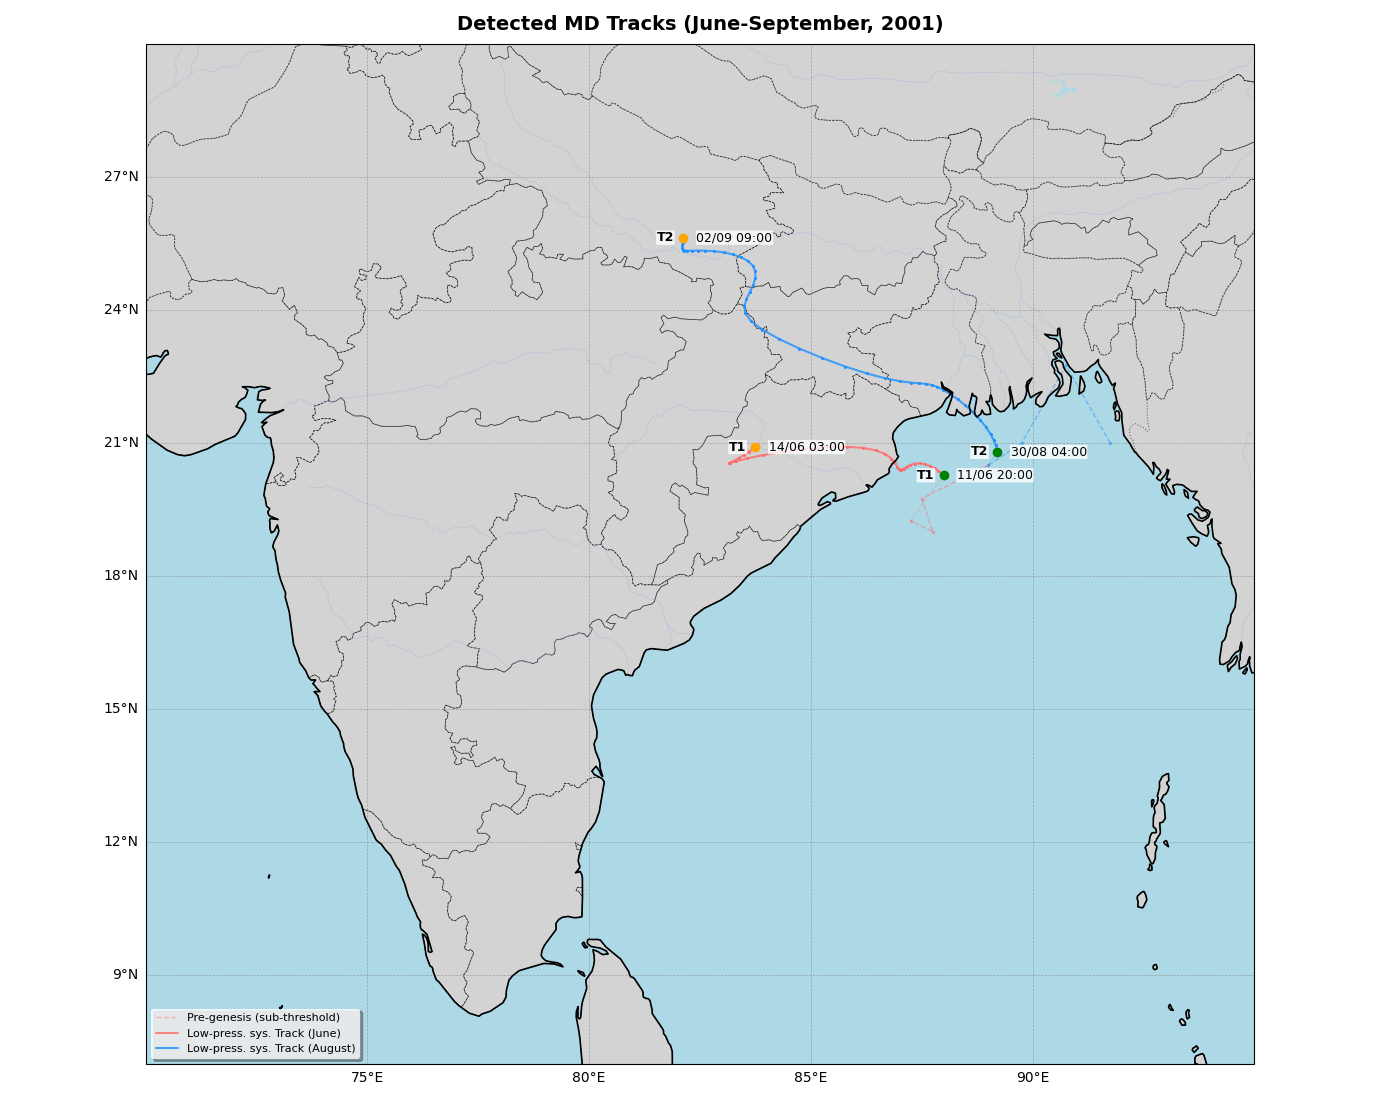
\includegraphics[width=0.67\textwidth]{MD_tracks_2001.png}
  \caption{2001 Monsoon Season}
  \label{fig:tracks_2001}
\end{figure}

\clearpage

\begin{figure}[p]
  \begin{adjustwidth}{-2.4cm}{0cm}
    \centering
    \begin{subfigure}{0.52\textwidth}
      \centering
      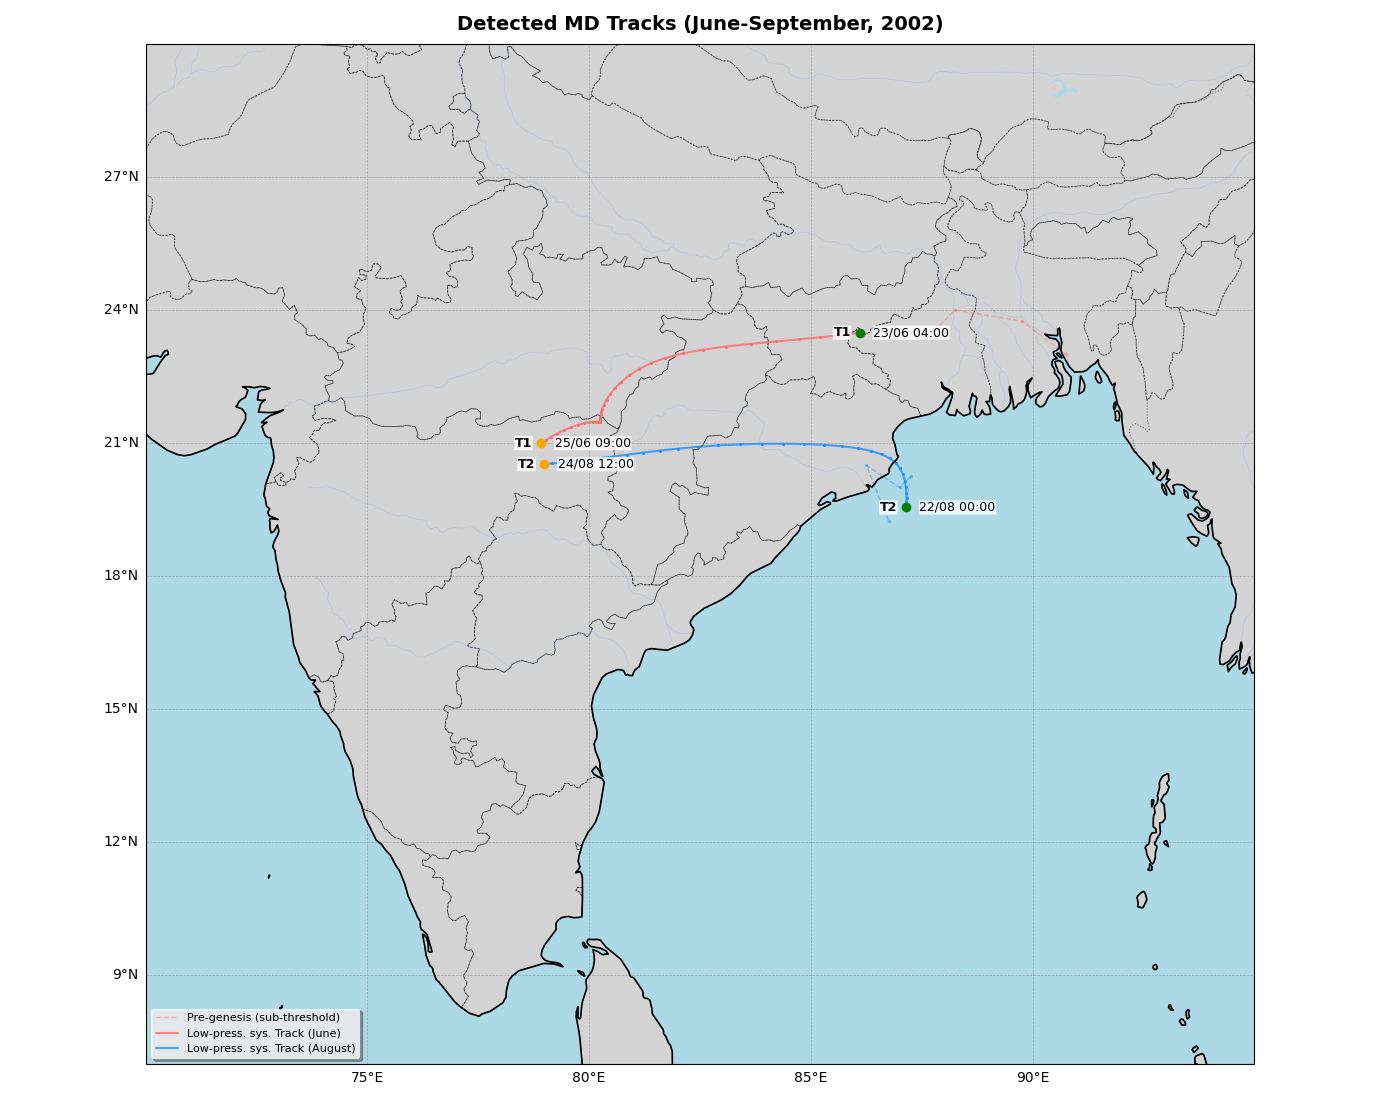
\includegraphics[width=1.2\textwidth]{MD_tracks_2002.png}
      \caption{2002 Monsoon Season}
    \end{subfigure}
    \hspace{0.11cm}
    \begin{subfigure}{0.52\textwidth}
      \centering
      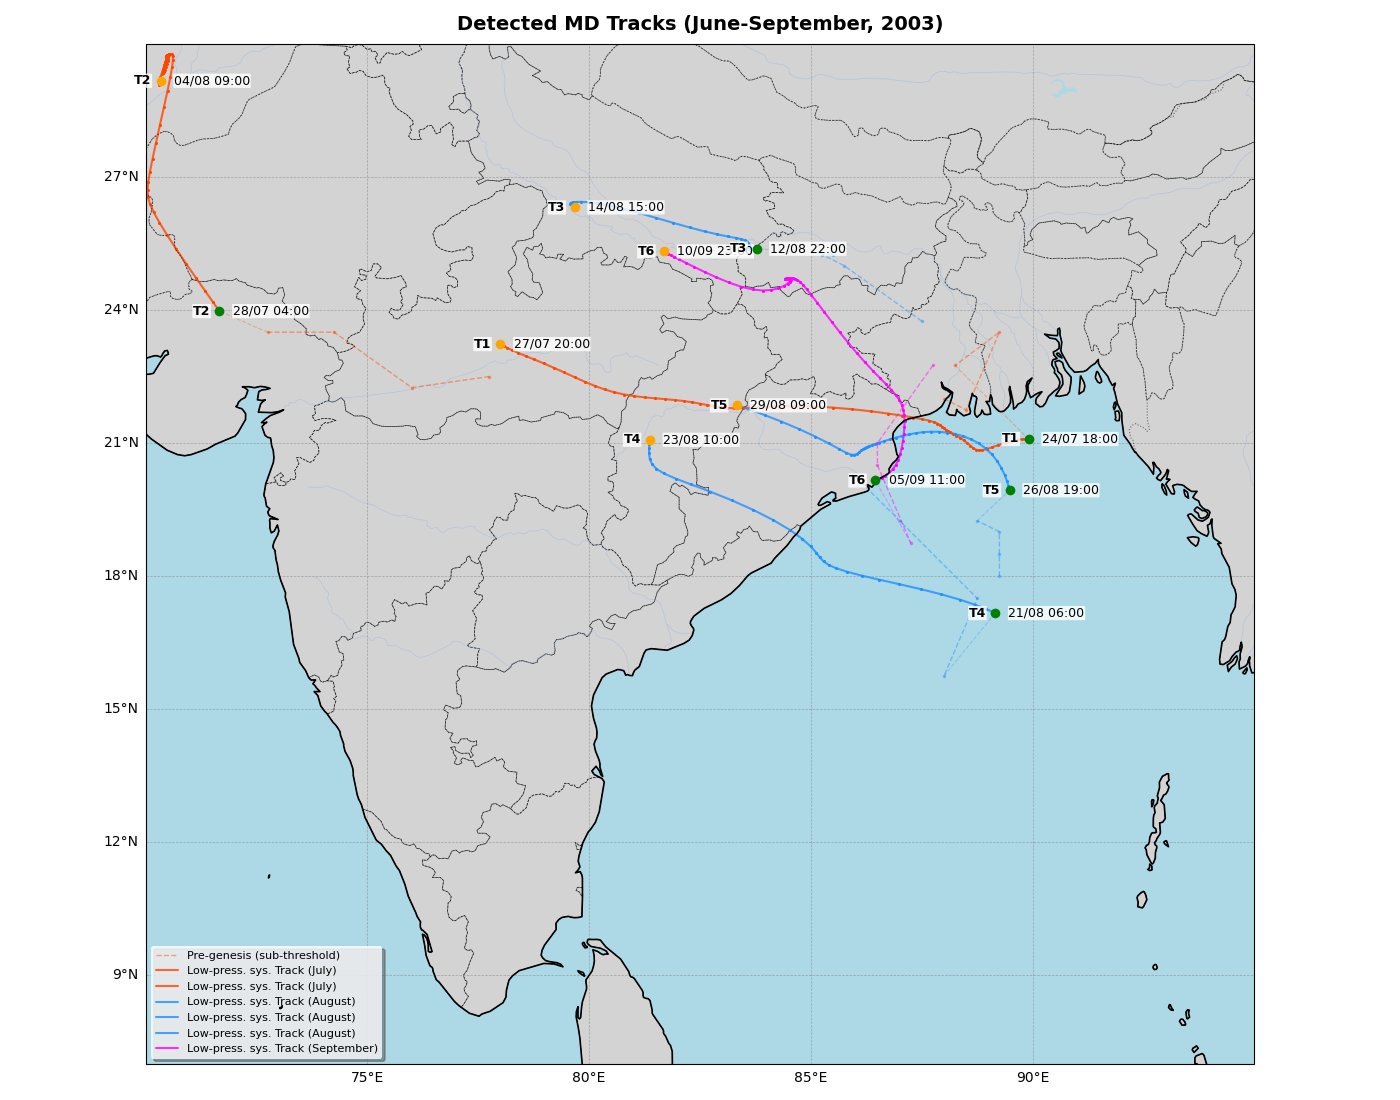
\includegraphics[width=1.2\textwidth]{MD_tracks_2003.png}
      \caption{2003 Monsoon Season}
    \end{subfigure}

    \vspace{0.9cm}

    \begin{subfigure}{0.52\textwidth}
      \centering
      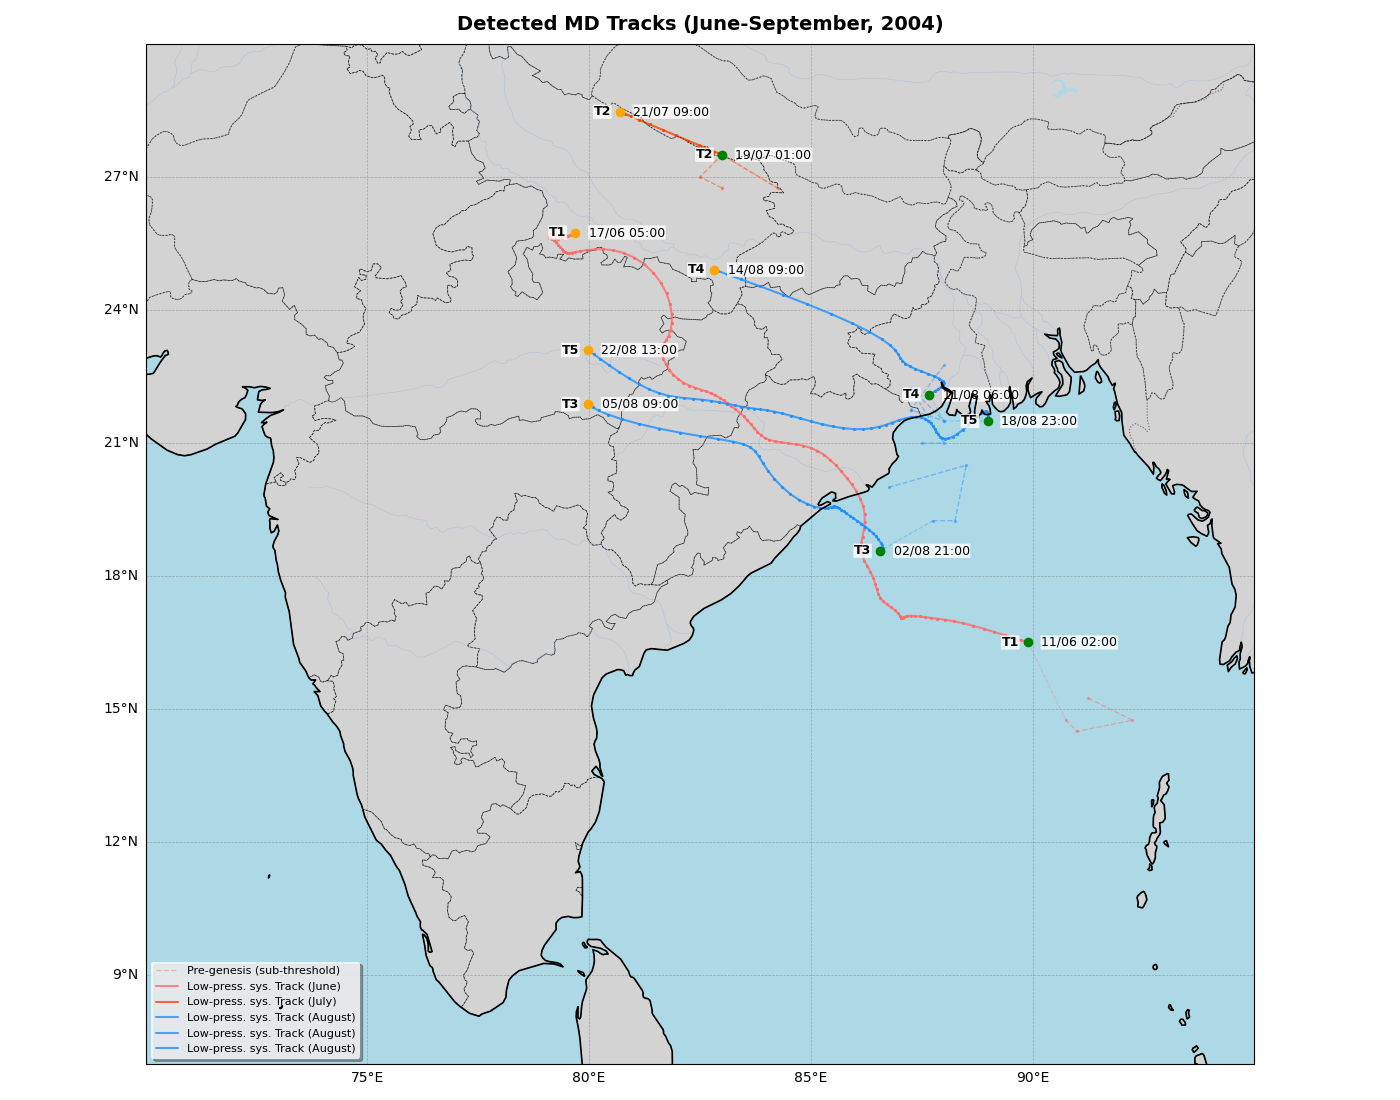
\includegraphics[width=1.2\textwidth]{MD_tracks_2004.png}
      \caption{2004 Monsoon Season}
    \end{subfigure}
    \hspace{0.11cm}
    \begin{subfigure}{0.52\textwidth}
      \centering
      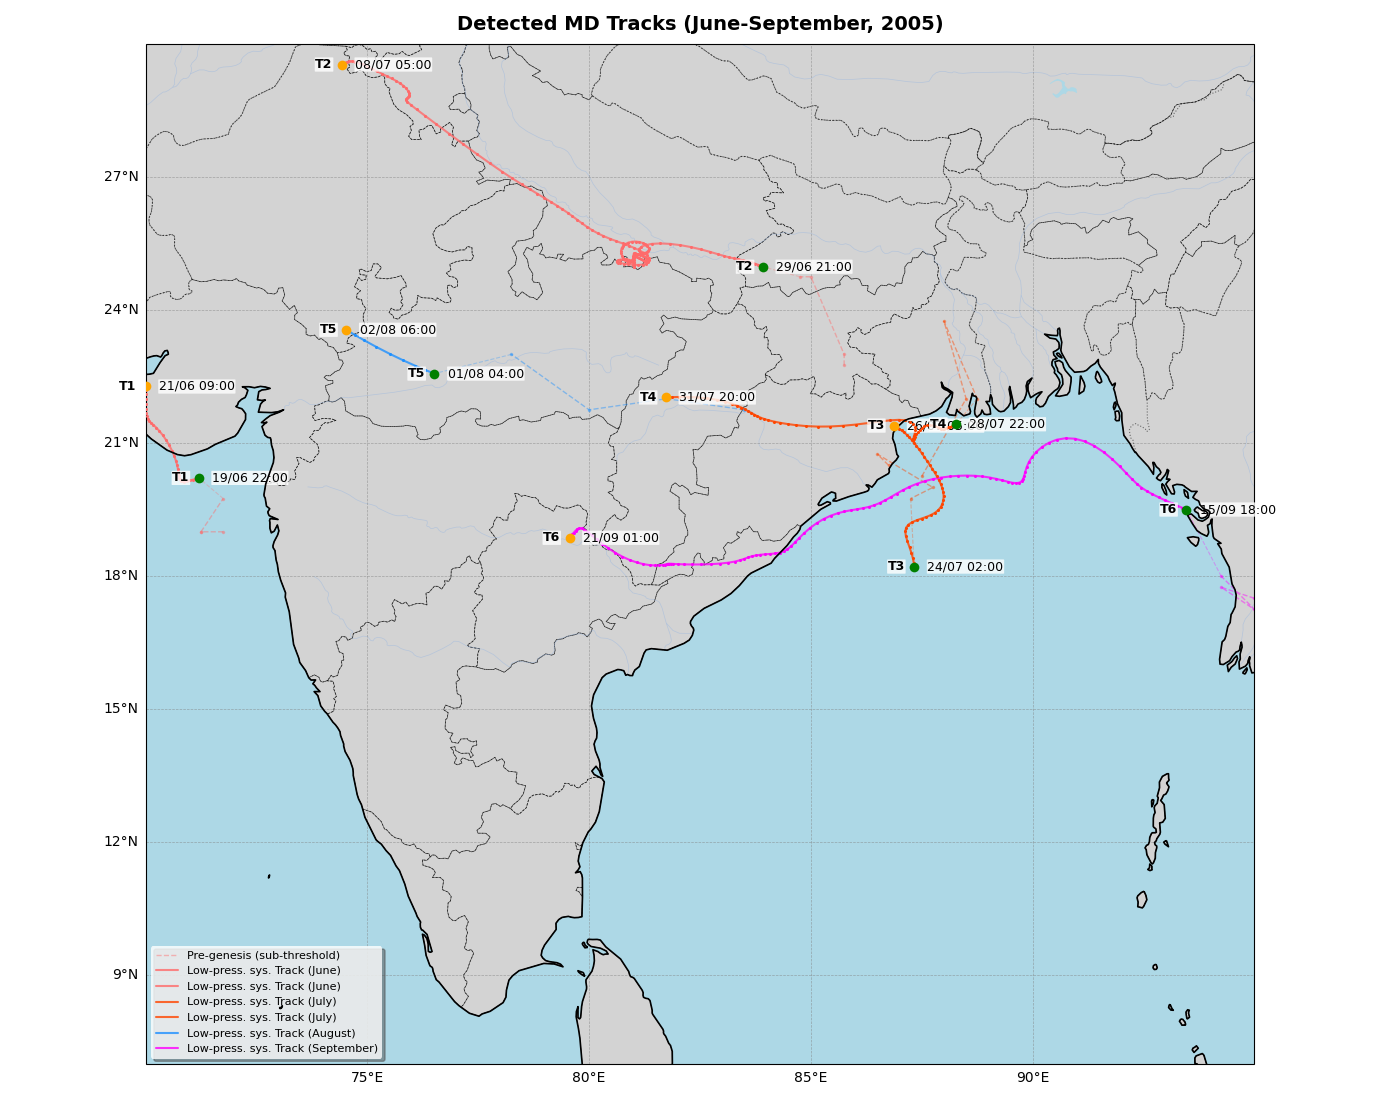
\includegraphics[width=1.2\textwidth]{MD_tracks_2005.png}
      \caption{2005 Monsoon Season}
    \end{subfigure}
    \caption{Annual MD Tracks: 2002-2005}
  \end{adjustwidth}
\end{figure}

\begin{figure}[p]
  \begin{adjustwidth}{-2.4cm}{0cm}
    \centering
    \begin{subfigure}{0.52\textwidth}
      \centering
      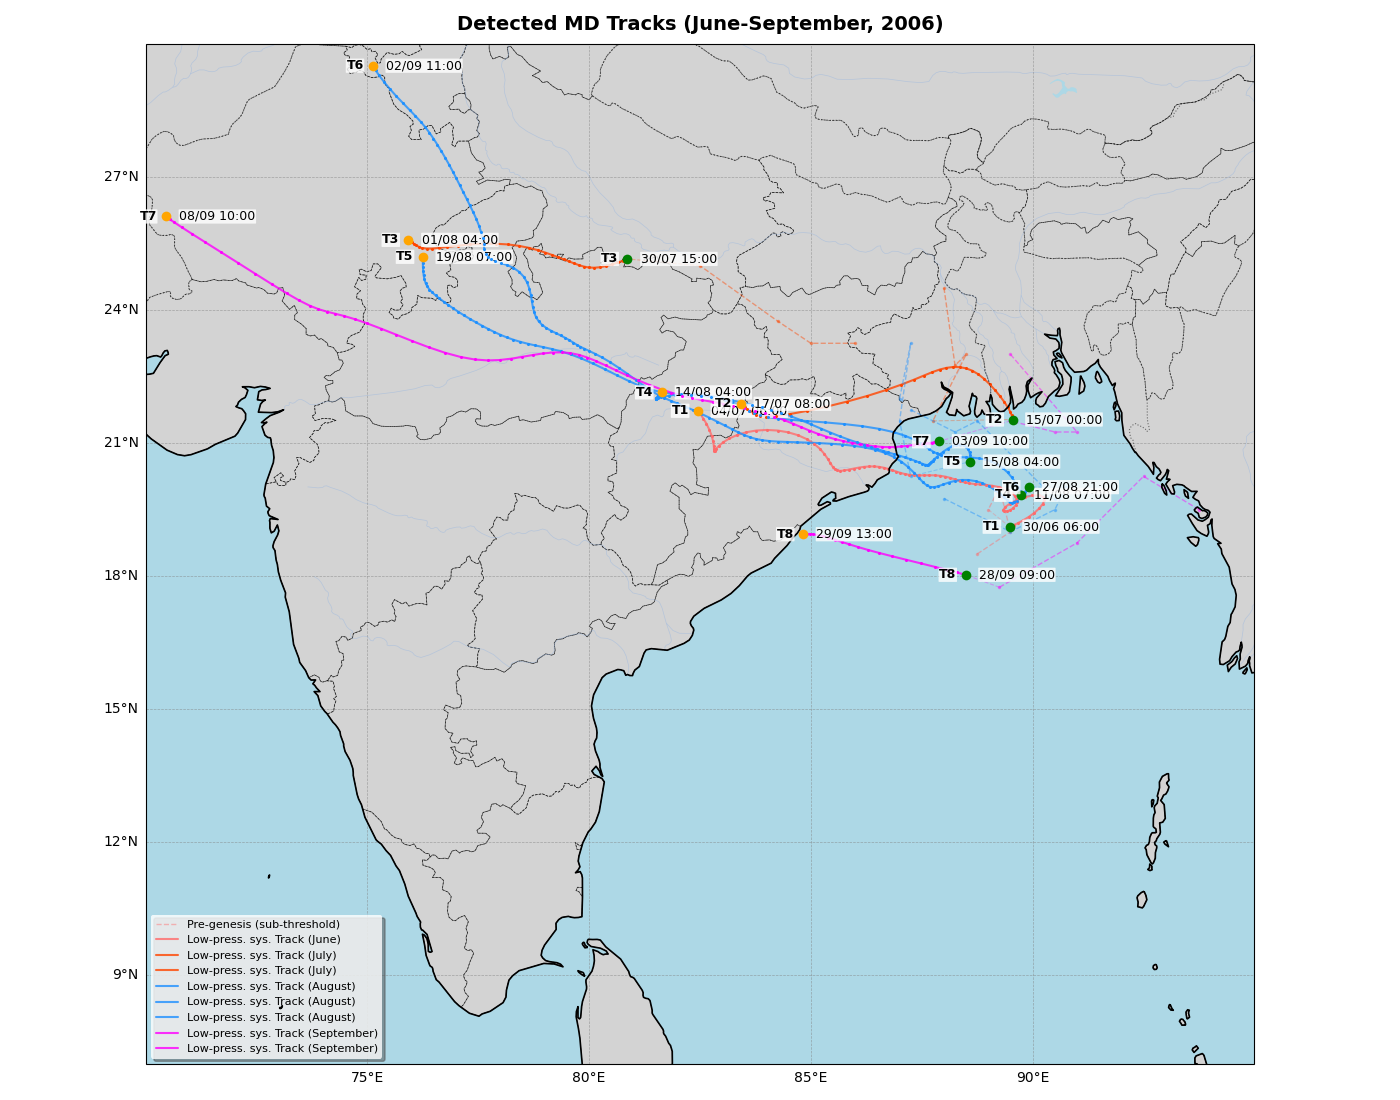
\includegraphics[width=1.2\textwidth]{MD_tracks_2006.png}
      \caption{2006 Monsoon Season}
    \end{subfigure}
    \hspace{0.11cm}
    \begin{subfigure}{0.52\textwidth}
      \centering
      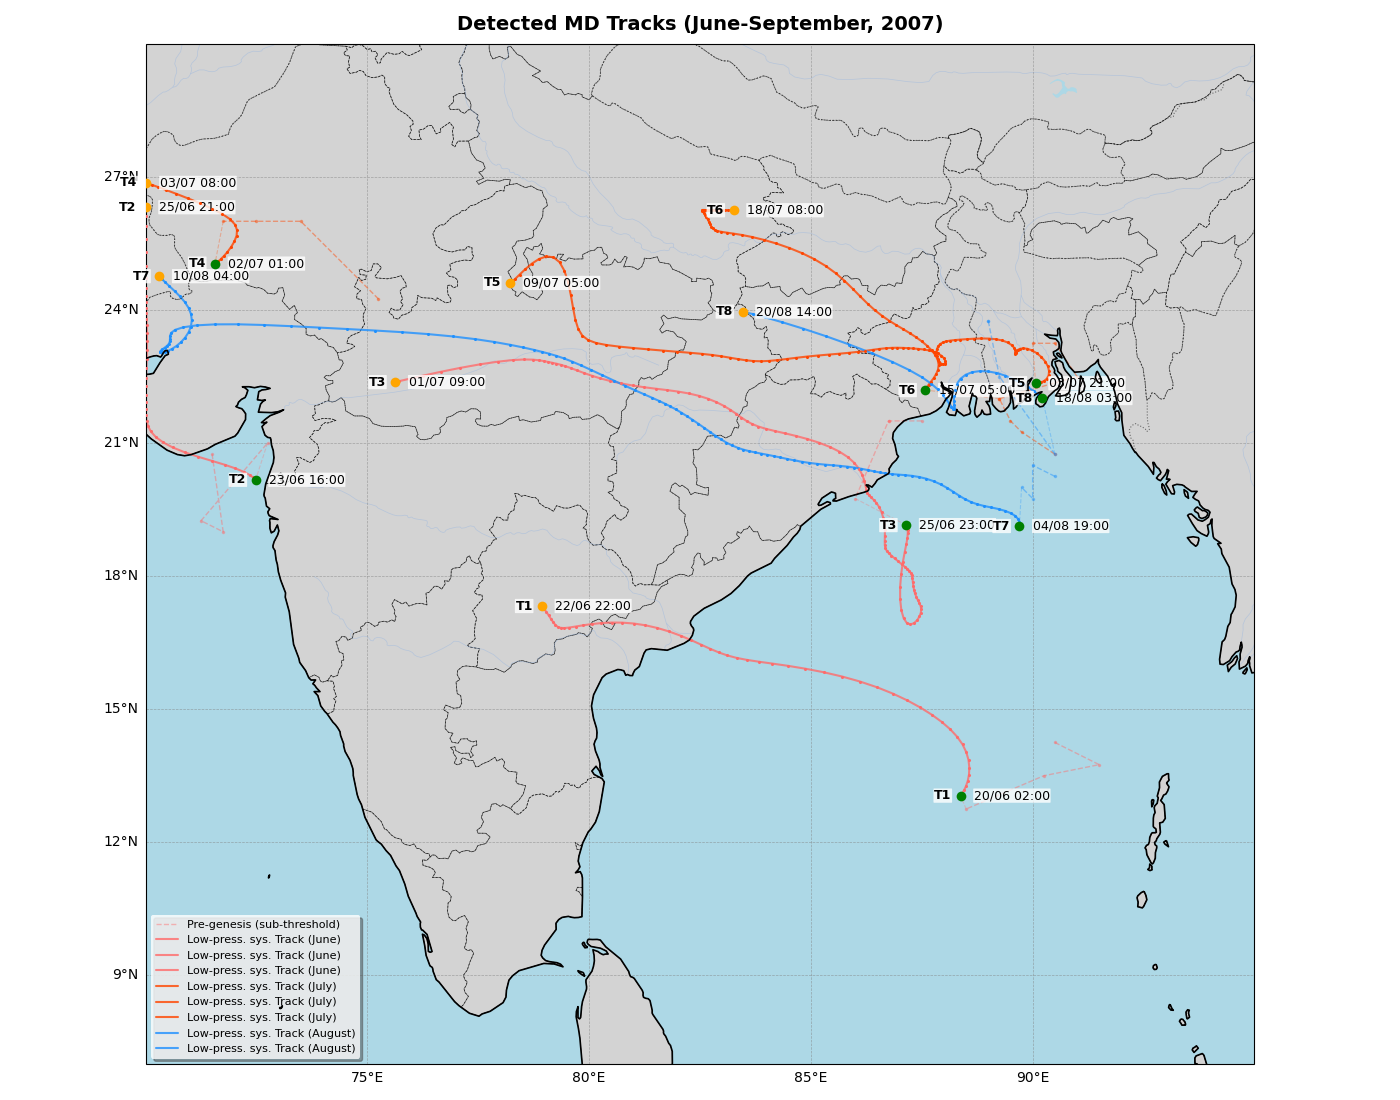
\includegraphics[width=1.2\textwidth]{MD_tracks_2007.png}
      \caption{2007 Monsoon Season}
    \end{subfigure}

    \vspace{0.9cm}

    \begin{subfigure}{0.52\textwidth}
      \centering
      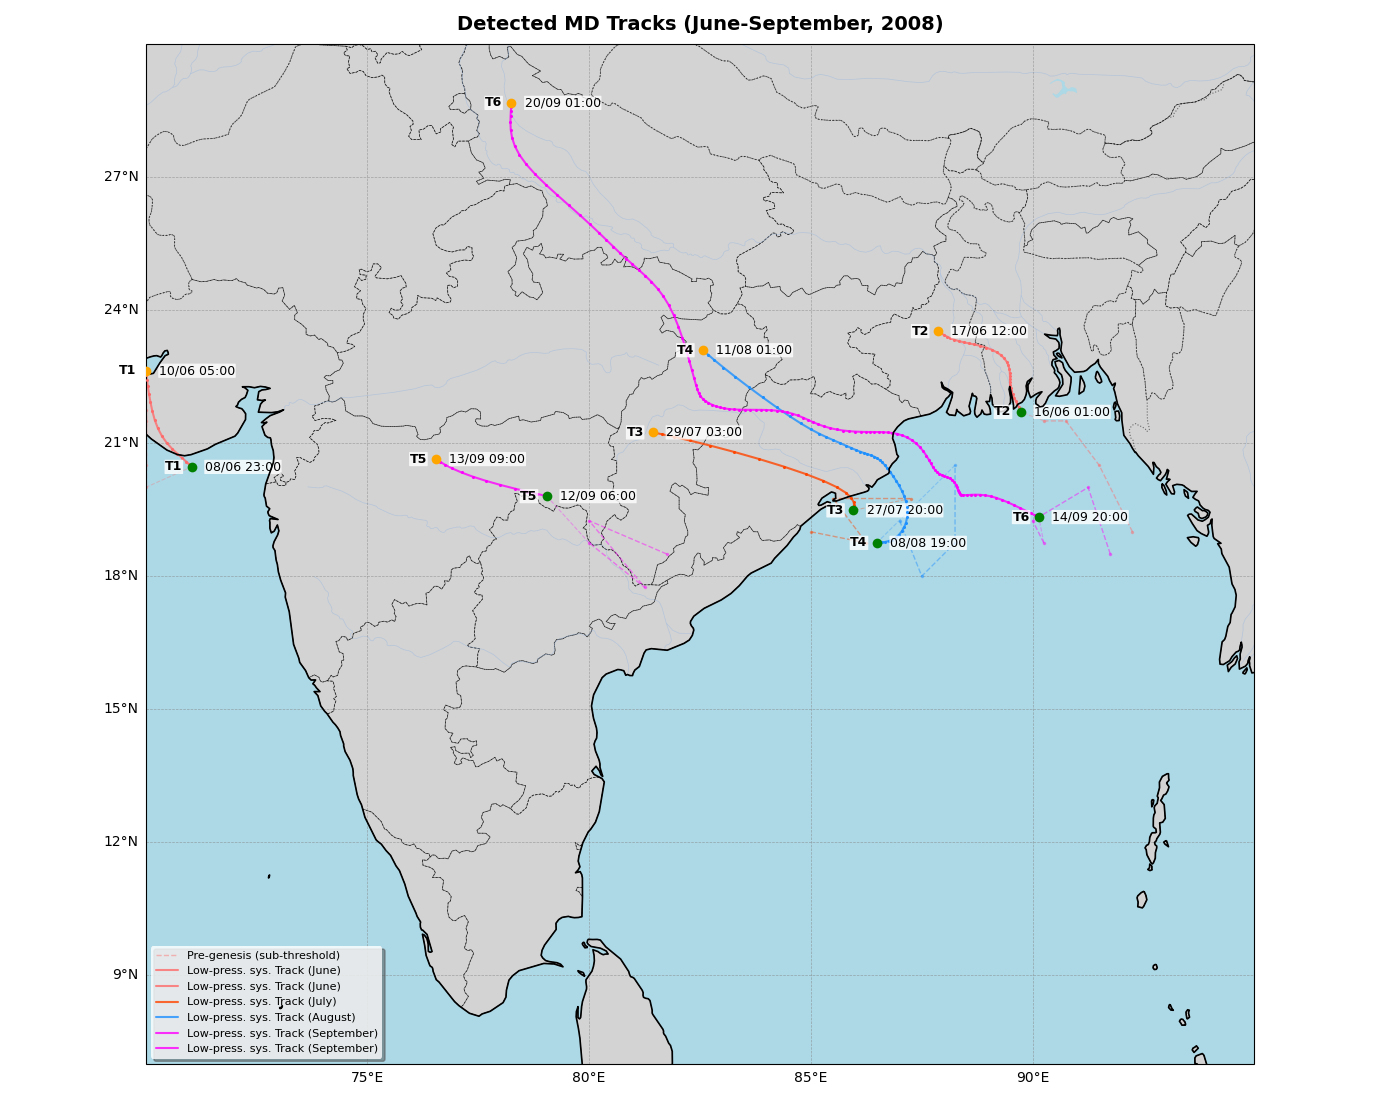
\includegraphics[width=1.2\textwidth]{MD_tracks_2008.png}
      \caption{2008 Monsoon Season}
    \end{subfigure}
    \hspace{0.11cm}
    \begin{subfigure}{0.52\textwidth}
      \centering
      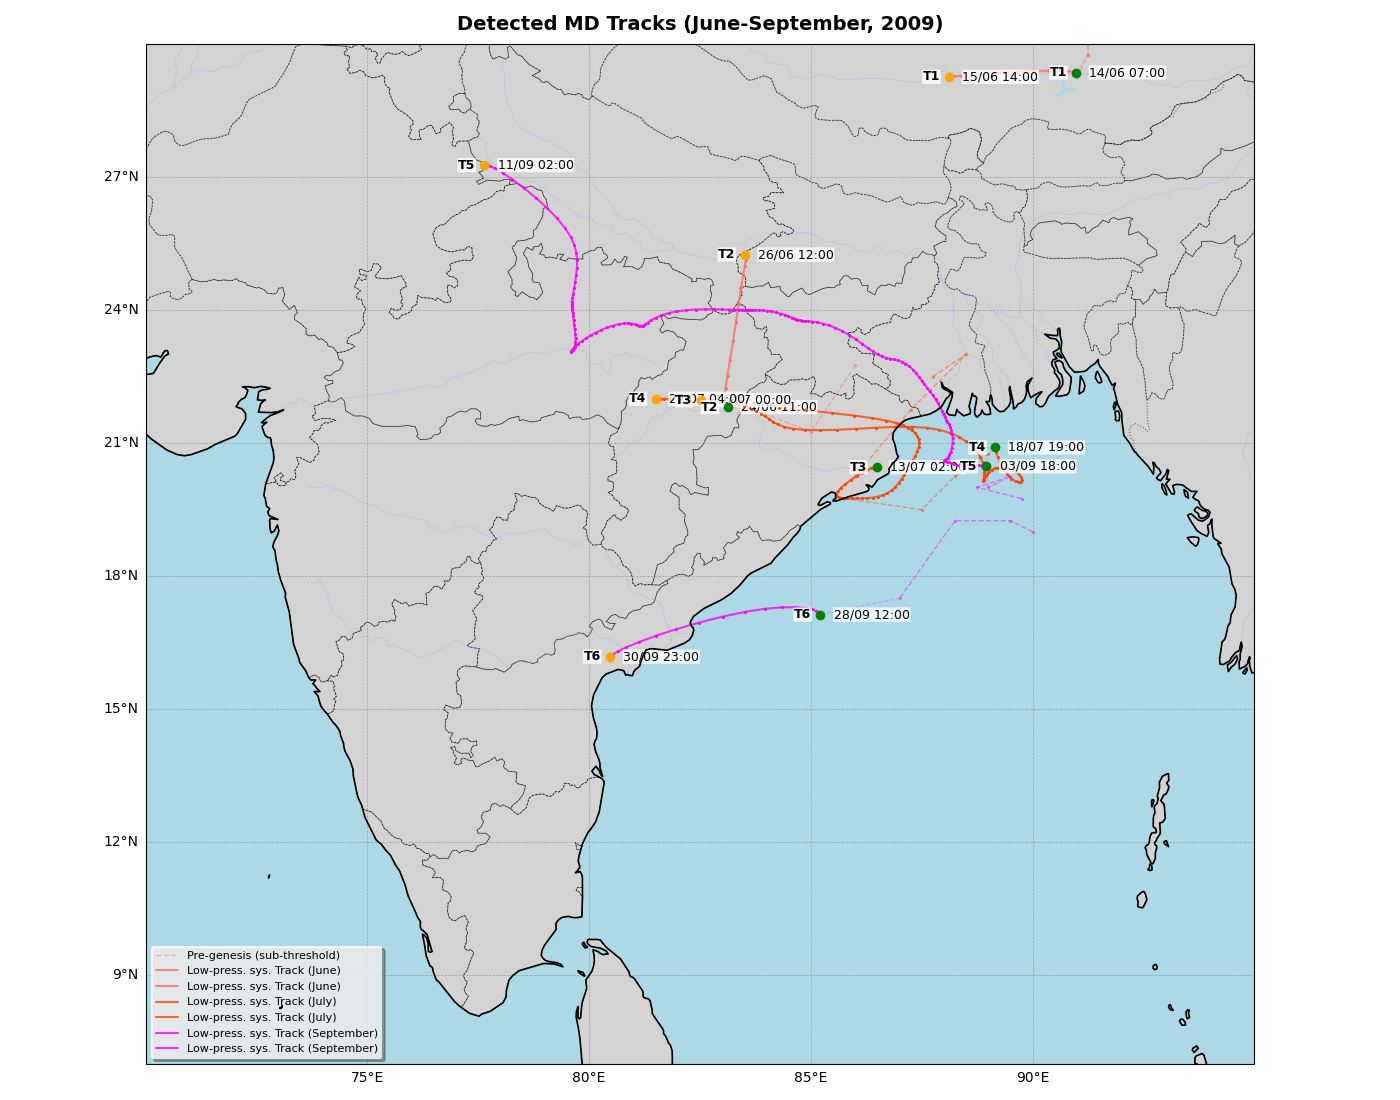
\includegraphics[width=1.2\textwidth]{MD_tracks_2009.png}
      \caption{2009 Monsoon Season}
    \end{subfigure}
    \caption{Annual MD Tracks: 2006-2009}
  \end{adjustwidth}
\end{figure}

\begin{figure}[p]
  \begin{adjustwidth}{-2.4cm}{0cm}
    \centering
    \begin{subfigure}{0.52\textwidth}
      \centering
      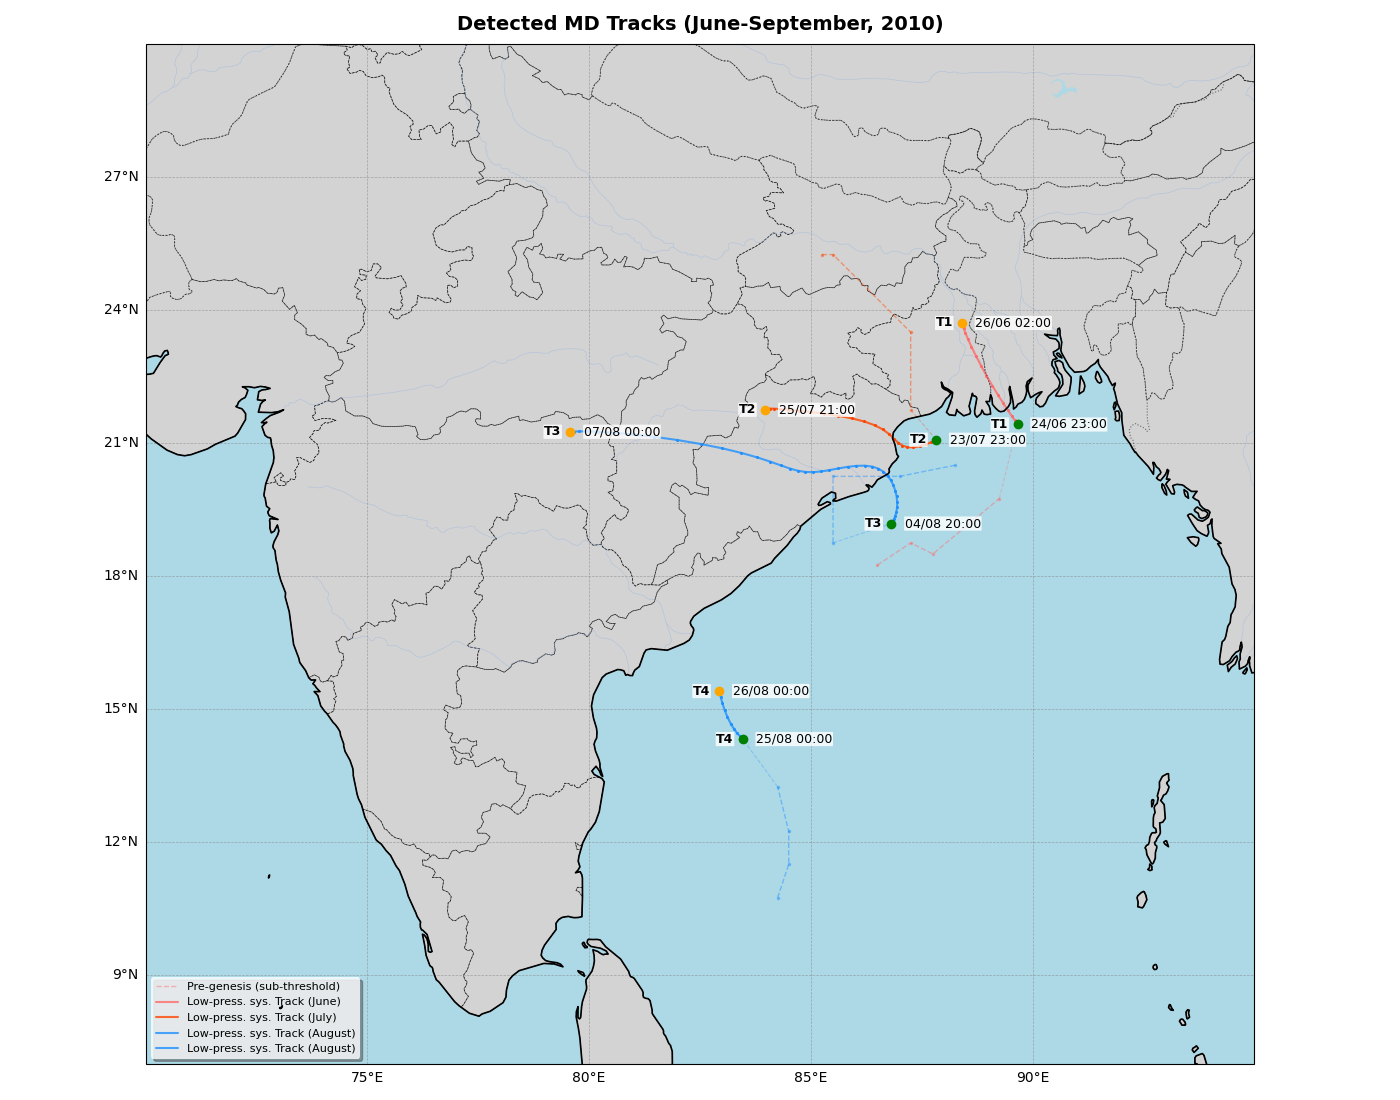
\includegraphics[width=1.2\textwidth]{MD_tracks_2010.png}
      \caption{2010 Monsoon Season}
    \end{subfigure}
    \hspace{0.11cm}
    \begin{subfigure}{0.52\textwidth}
      \centering
      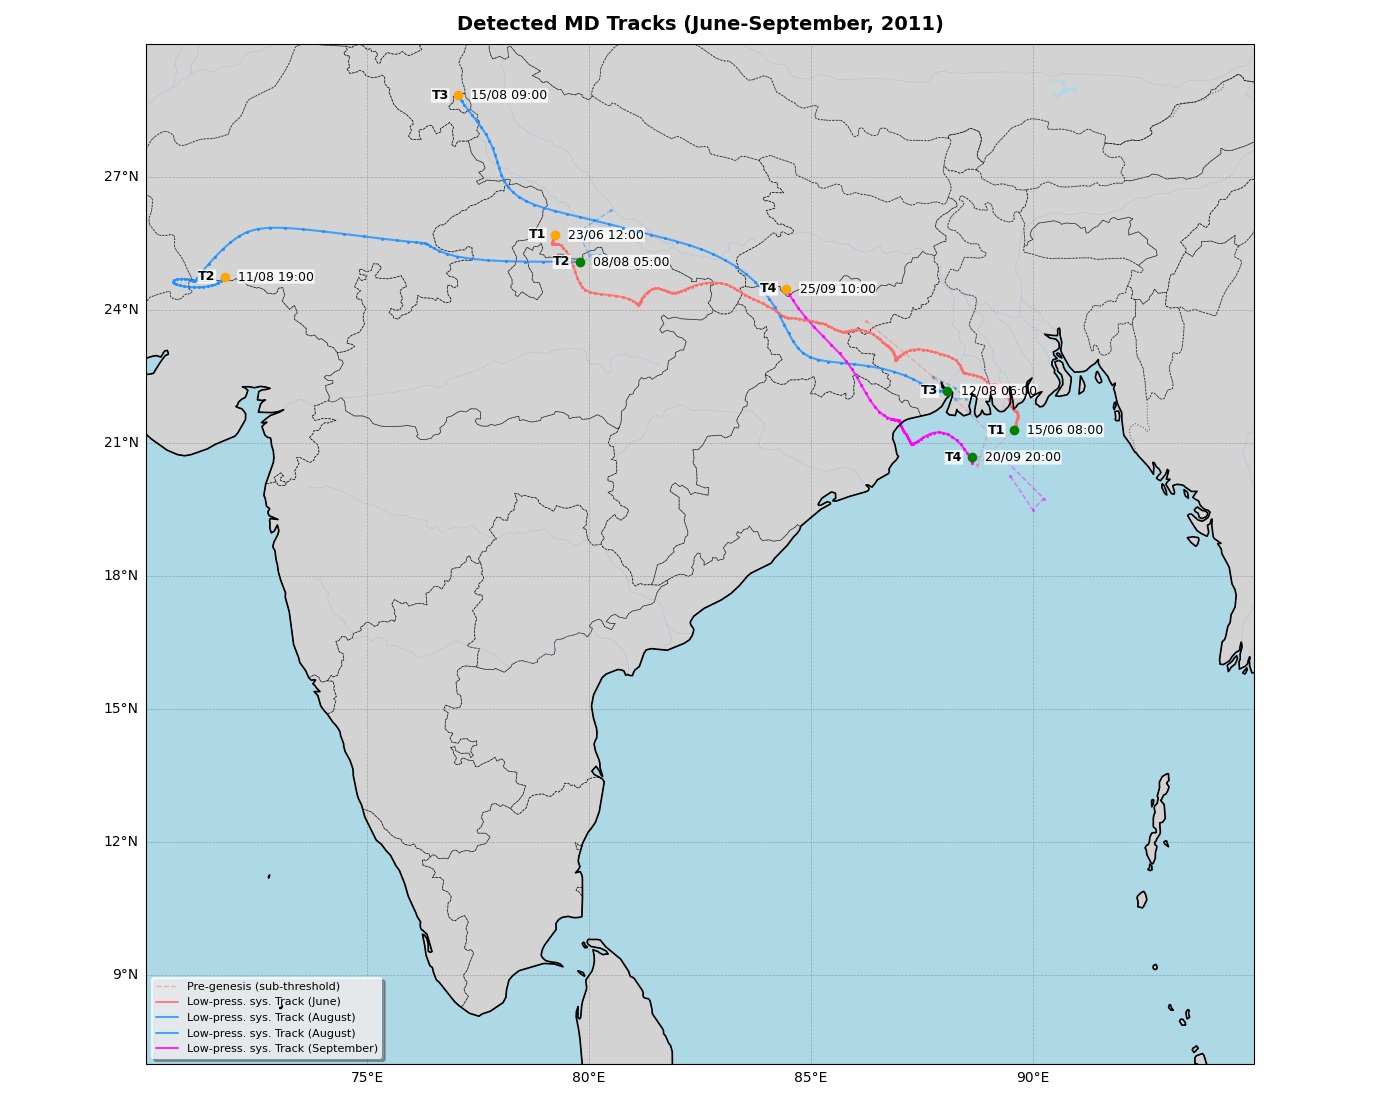
\includegraphics[width=1.2\textwidth]{MD_tracks_2011.png}
      \caption{2011 Monsoon Season}
    \end{subfigure}

    \vspace{0.9cm}

    \begin{subfigure}{0.52\textwidth}
      \centering
      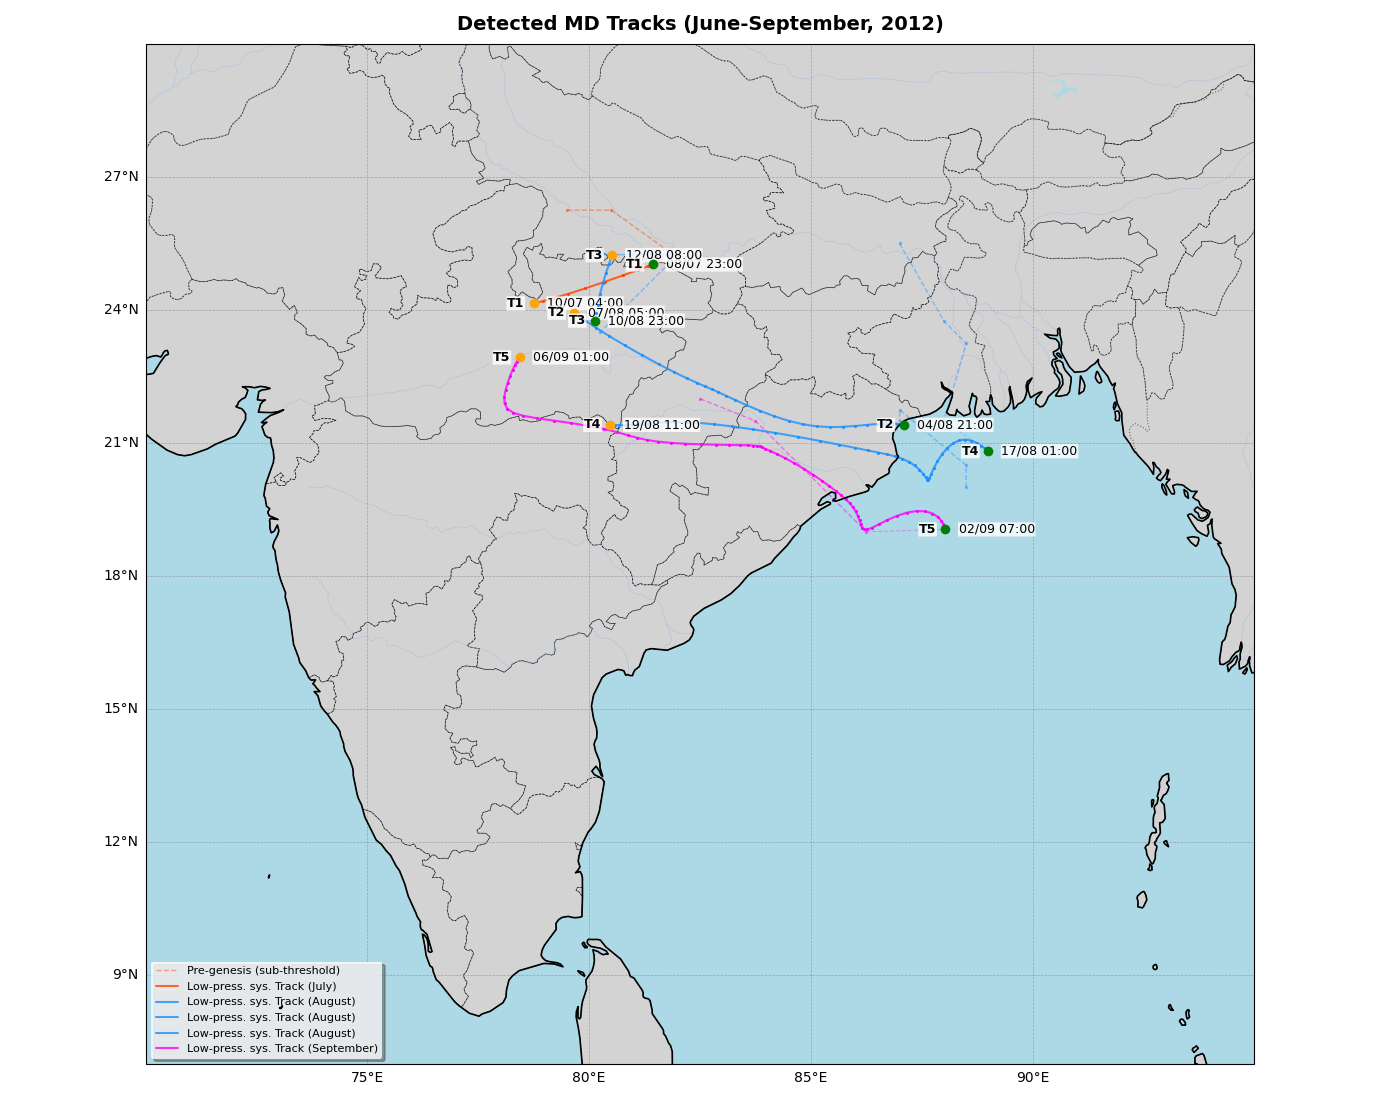
\includegraphics[width=1.2\textwidth]{MD_tracks_2012.png}
      \caption{2012 Monsoon Season}
    \end{subfigure}
    \hspace{0.11cm}
    \begin{subfigure}{0.52\textwidth}
      \centering
      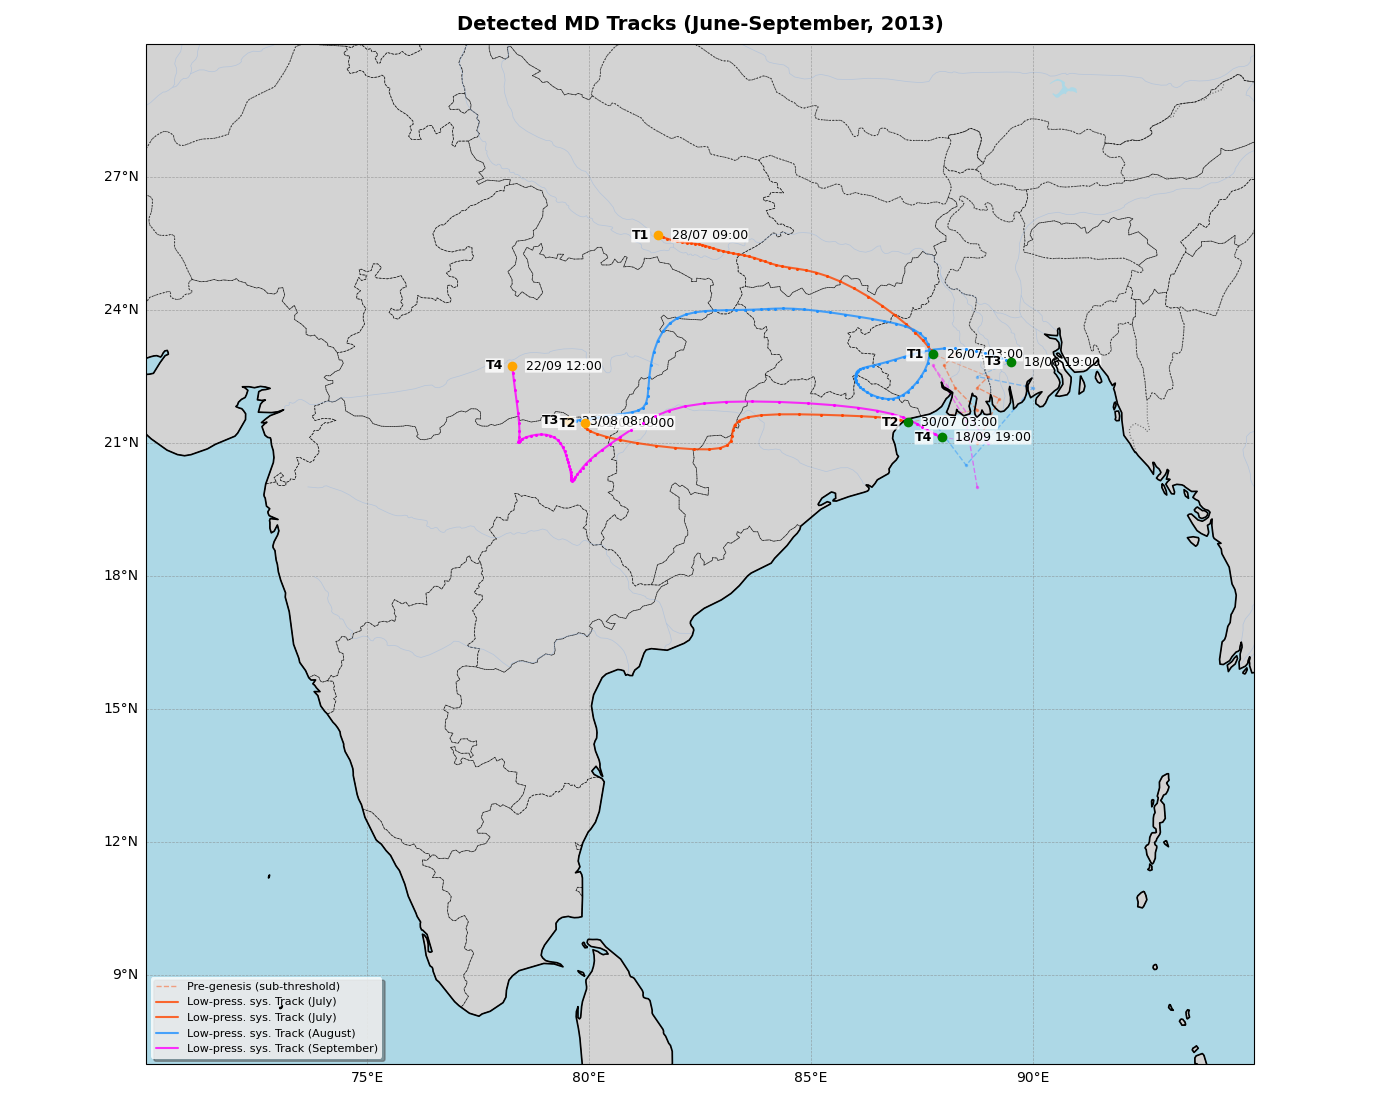
\includegraphics[width=1.2\textwidth]{MD_tracks_2013.png}
      \caption{2013 Monsoon Season}
    \end{subfigure}
    \caption{Annual MD Tracks: 2010-2013}
  \end{adjustwidth}
\end{figure}

\begin{figure}[p]
  \begin{adjustwidth}{-2.4cm}{0cm}
    \centering
    \begin{subfigure}{0.52\textwidth}
      \centering
      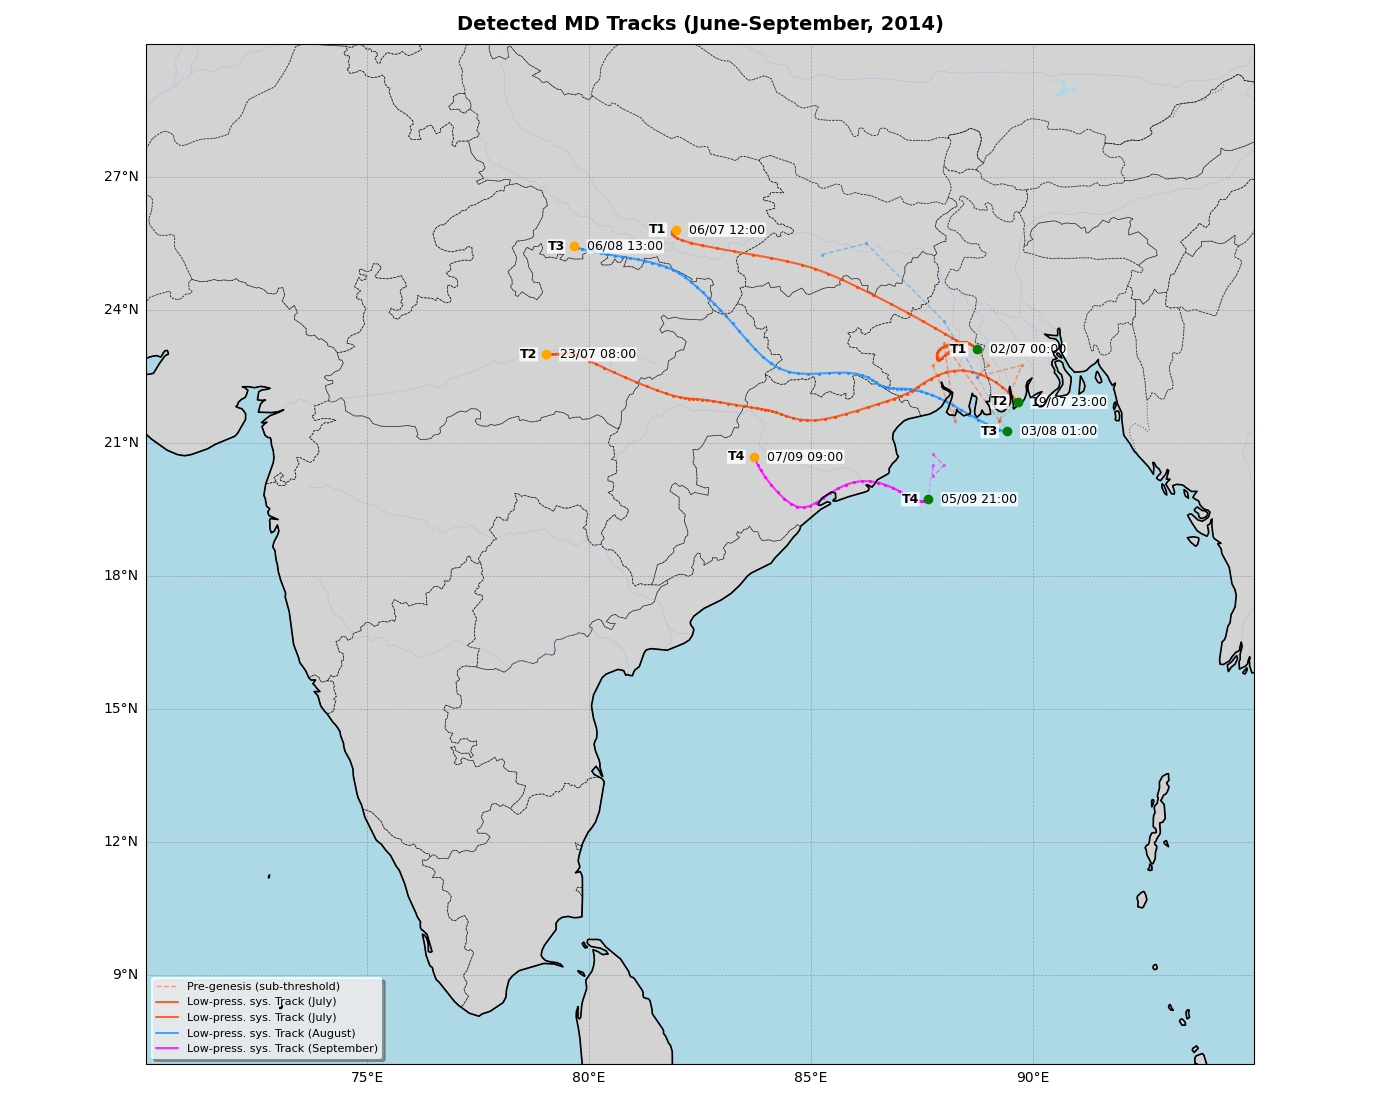
\includegraphics[width=1.2\textwidth]{MD_tracks_2014.png}
      \caption{2014 Monsoon Season}
    \end{subfigure}
    \hspace{0.11cm}
    \begin{subfigure}{0.52\textwidth}
      \centering
      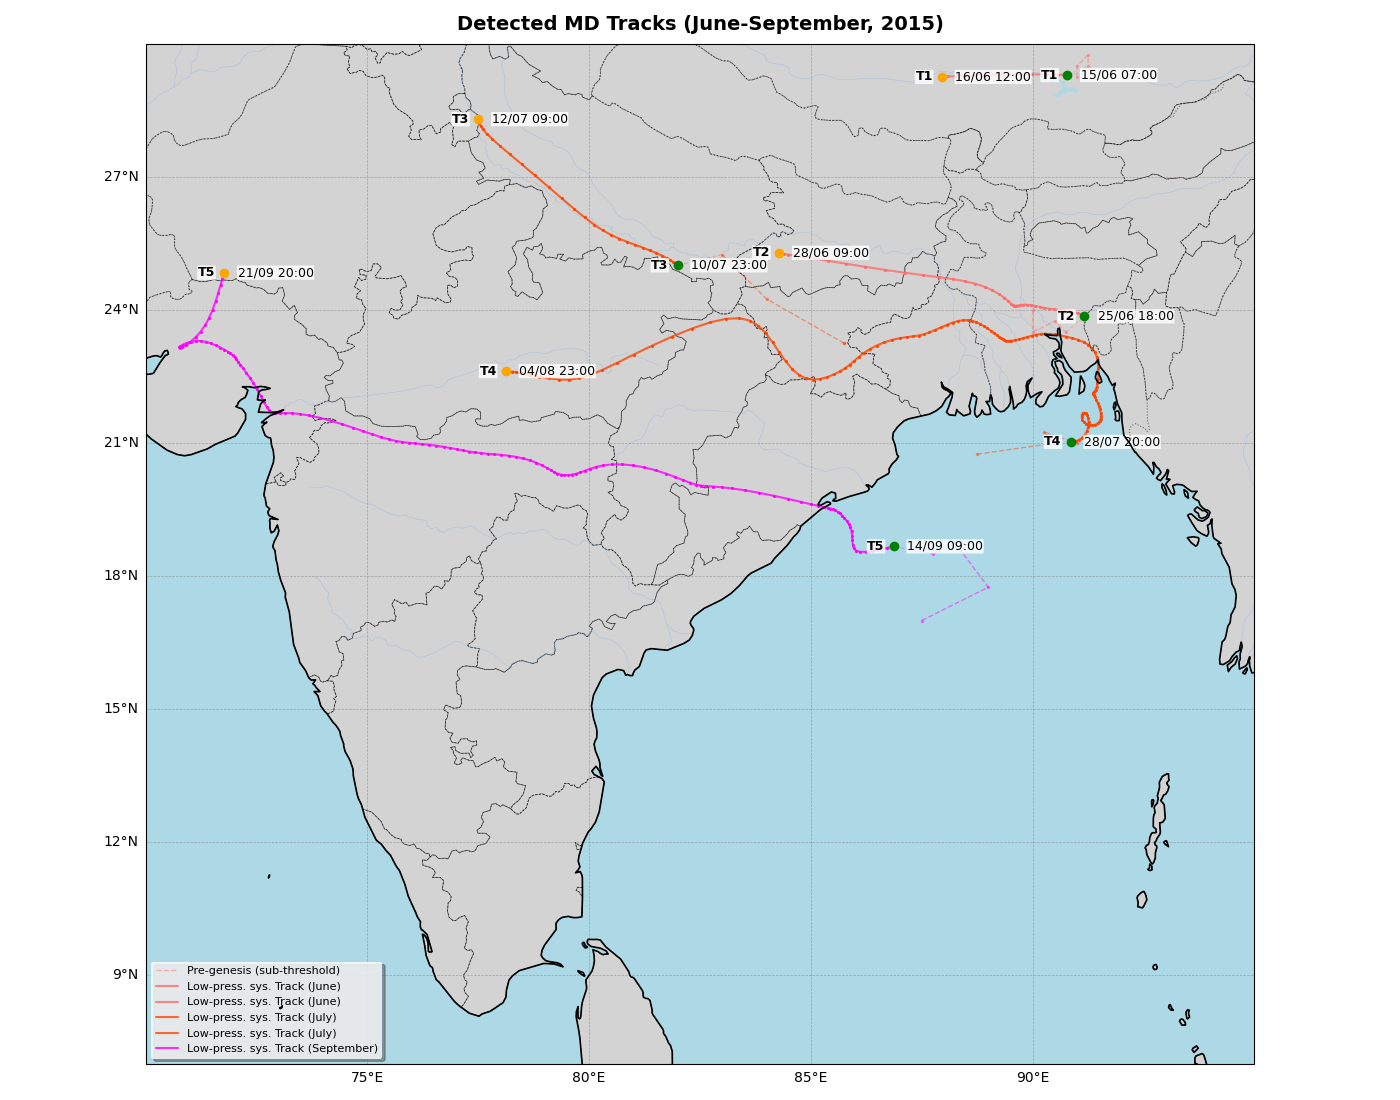
\includegraphics[width=1.2\textwidth]{MD_tracks_2015.png}
      \caption{2015 Monsoon Season}
    \end{subfigure}

    \vspace{0.9cm}

    \begin{subfigure}{0.52\textwidth}
      \centering
      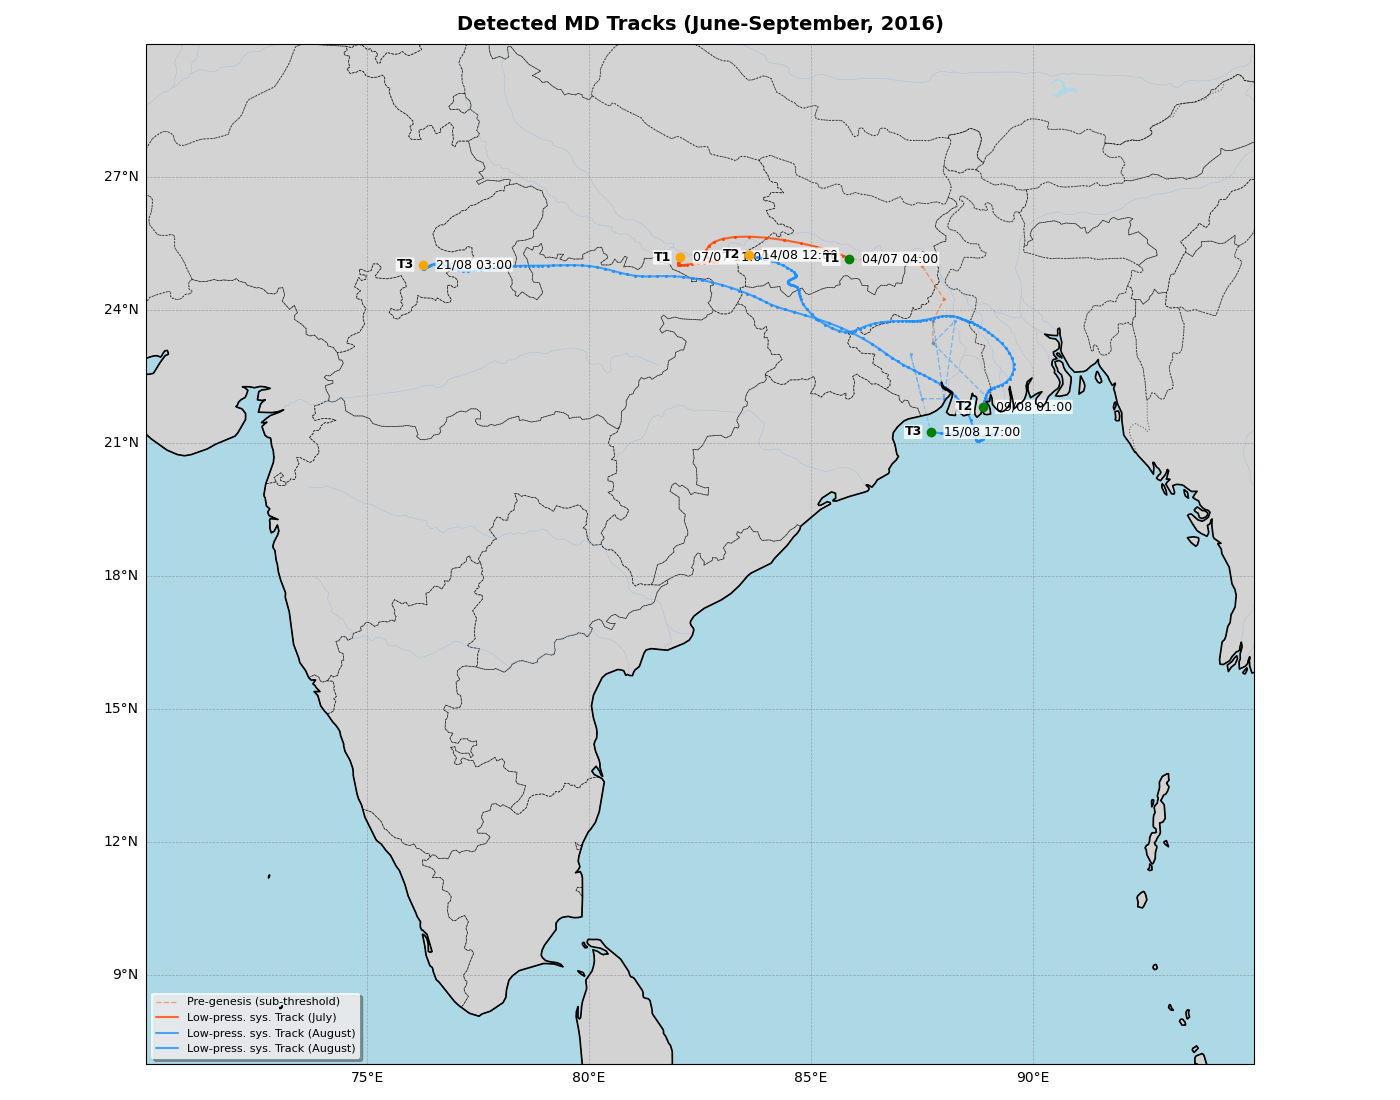
\includegraphics[width=1.2\textwidth]{MD_tracks_2016.png}
      \caption{2016 Monsoon Season}
    \end{subfigure}
    \hspace{0.11cm}
    \begin{subfigure}{0.52\textwidth}
      \centering
      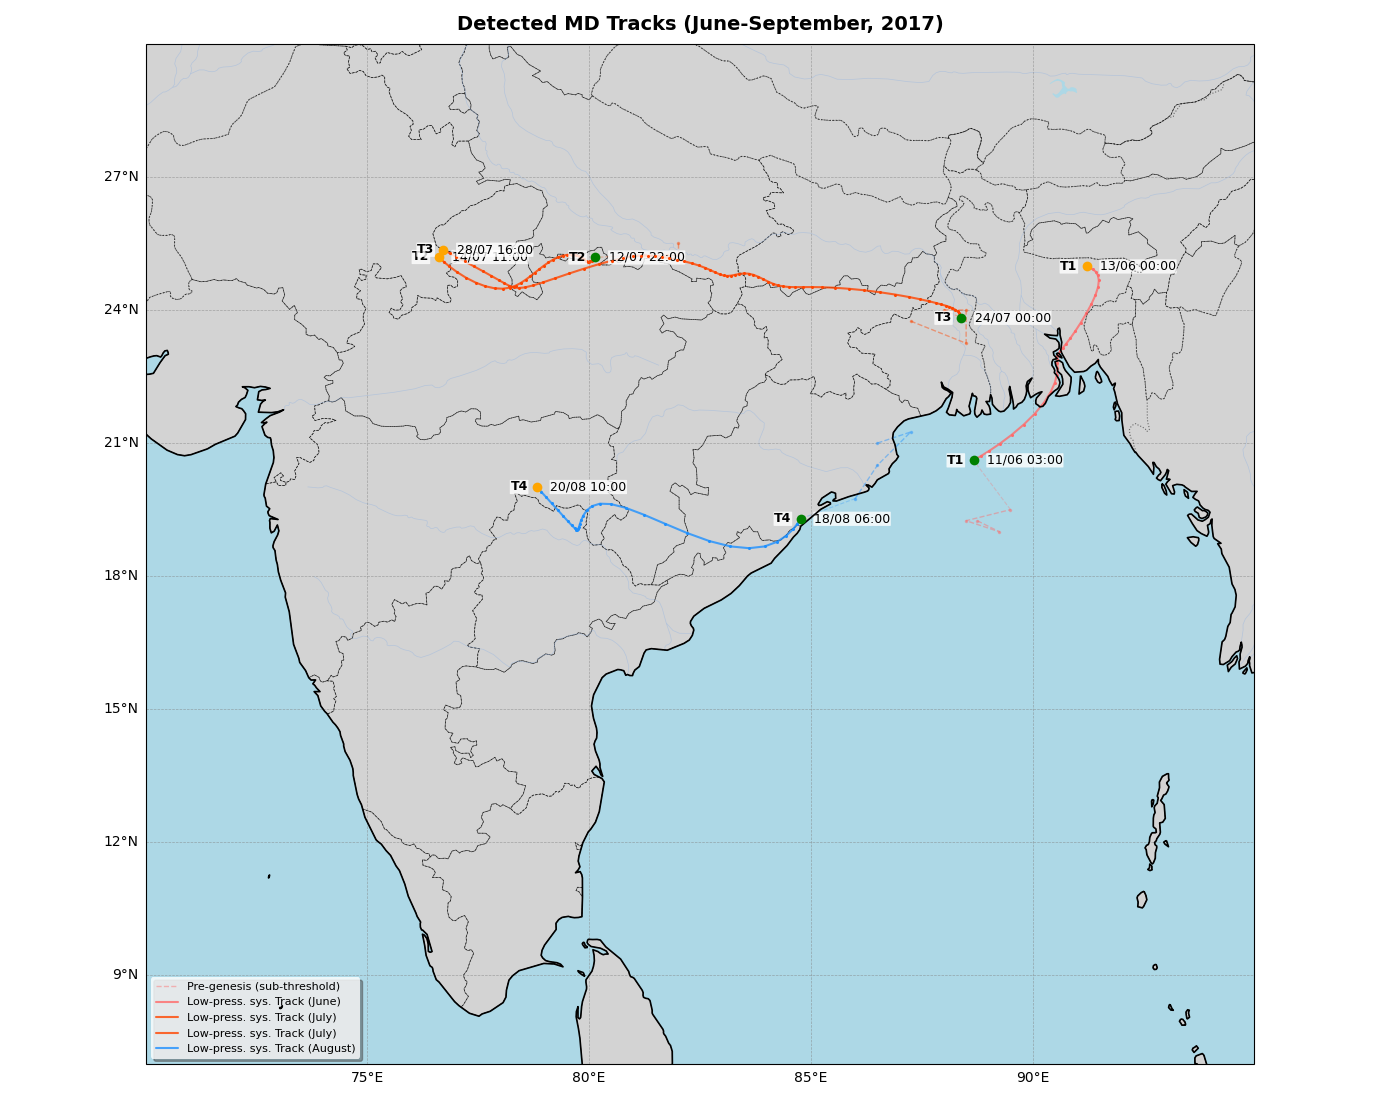
\includegraphics[width=1.2\textwidth]{MD_tracks_2017.png}
      \caption{2017 Monsoon Season}
    \end{subfigure}
    \caption{Annual MD Tracks: 2014-2017}
  \end{adjustwidth}
\end{figure}

\begin{figure}[p]
  \begin{adjustwidth}{-2.4cm}{0cm}
    \centering
    \begin{subfigure}{0.52\textwidth}
      \centering
      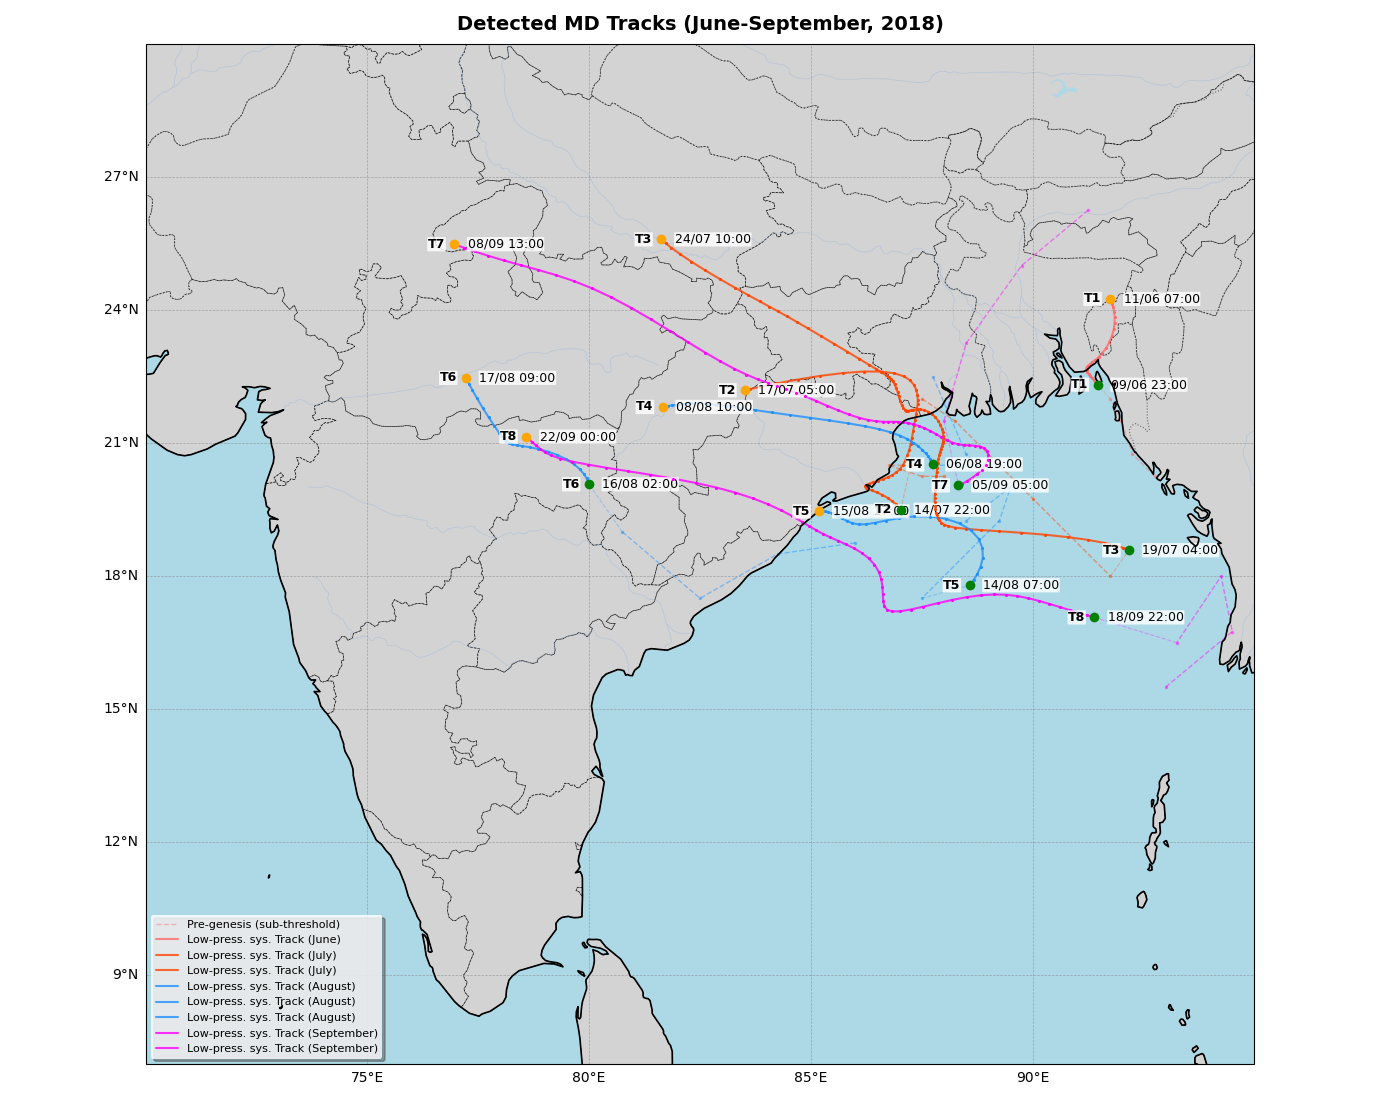
\includegraphics[width=1.2\textwidth]{MD_tracks_2018.png}
      \caption{2018 Monsoon Season}
    \end{subfigure}
    \hspace{0.11cm}
    \begin{subfigure}{0.52\textwidth}
      \centering
      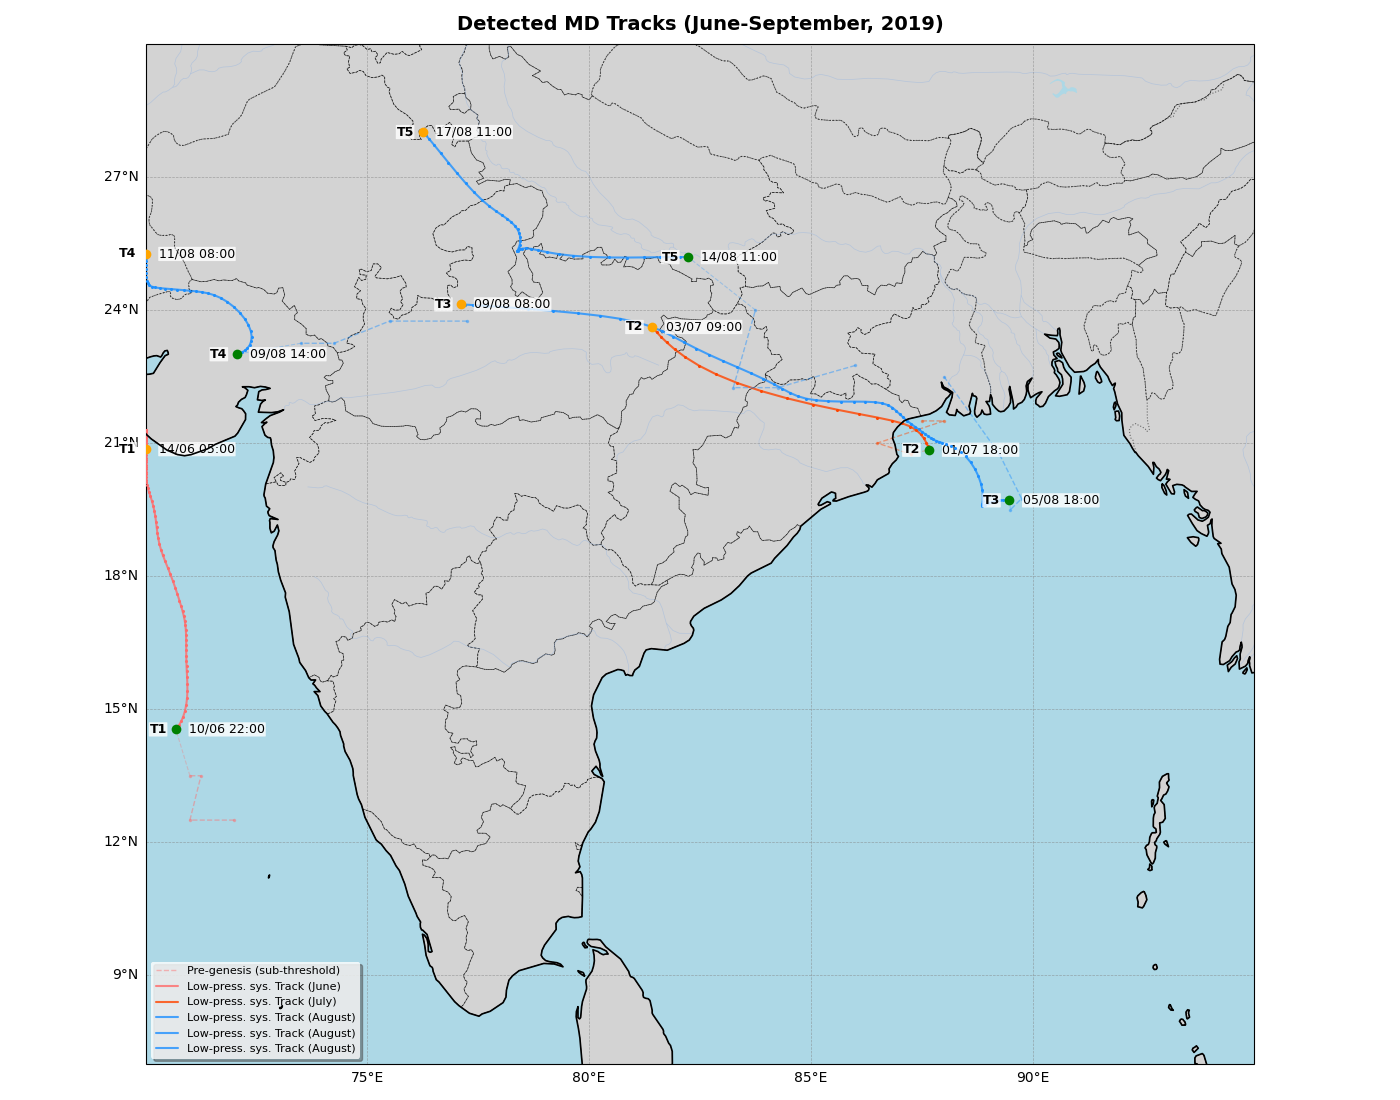
\includegraphics[width=1.2\textwidth]{MD_tracks_2019.png}
      \caption{2019 Monsoon Season}
    \end{subfigure}

    \vspace{0.9cm}

    \begin{subfigure}{0.52\textwidth}
      \centering
      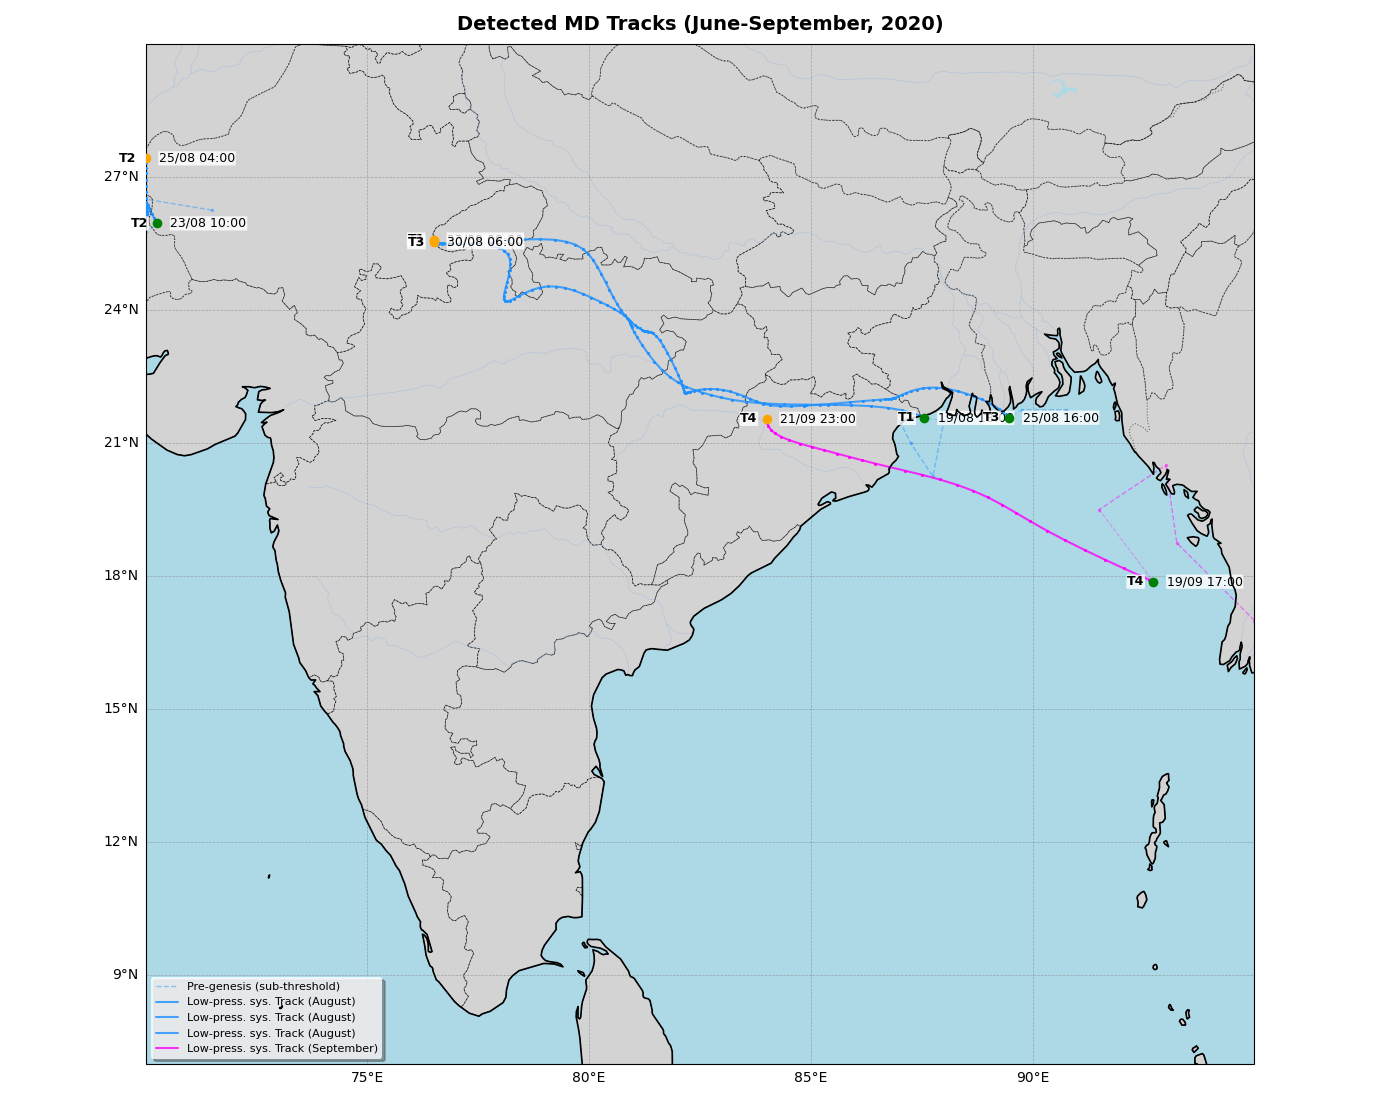
\includegraphics[width=1.2\textwidth]{MD_tracks_2020.png}
      \caption{2020 Monsoon Season}
    \end{subfigure}
    \hspace{0.11cm}
    \begin{subfigure}{0.52\textwidth}
      \centering
      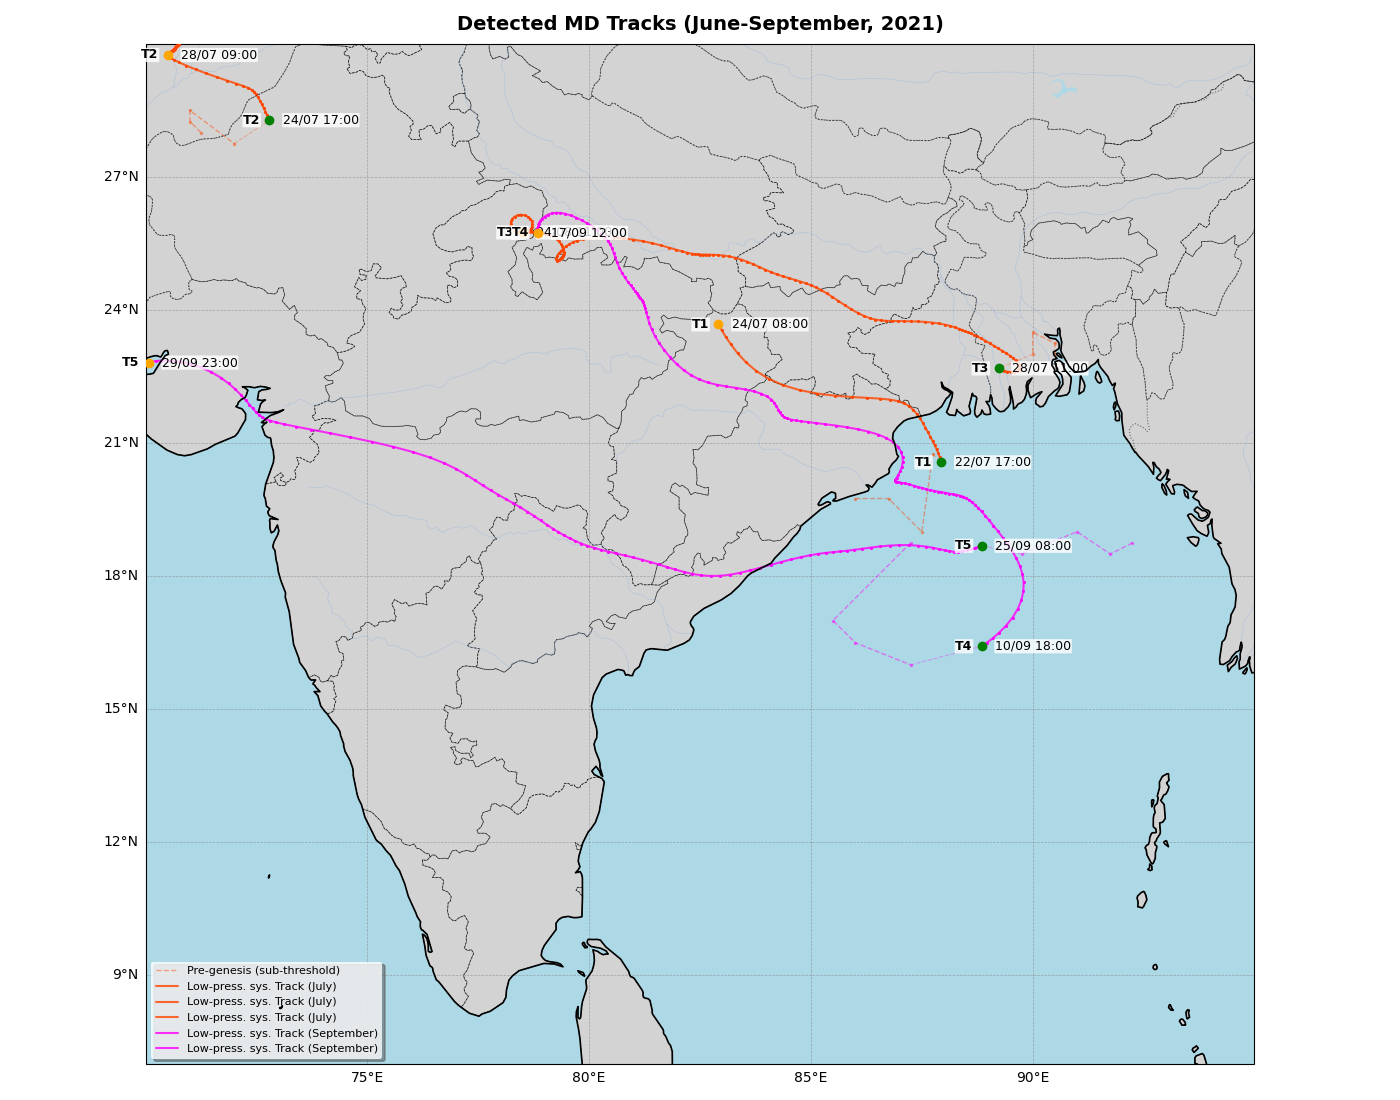
\includegraphics[width=1.2\textwidth]{MD_tracks_2021.png}
      \caption{2021 Monsoon Season}
    \end{subfigure}
    \caption{Annual MD Tracks: 2018-2021}
  \end{adjustwidth}
\end{figure}

\begin{figure}[p]
  \begin{adjustwidth}{-2.4cm}{0cm}
    \centering
    \begin{subfigure}{0.52\textwidth}
      \centering
      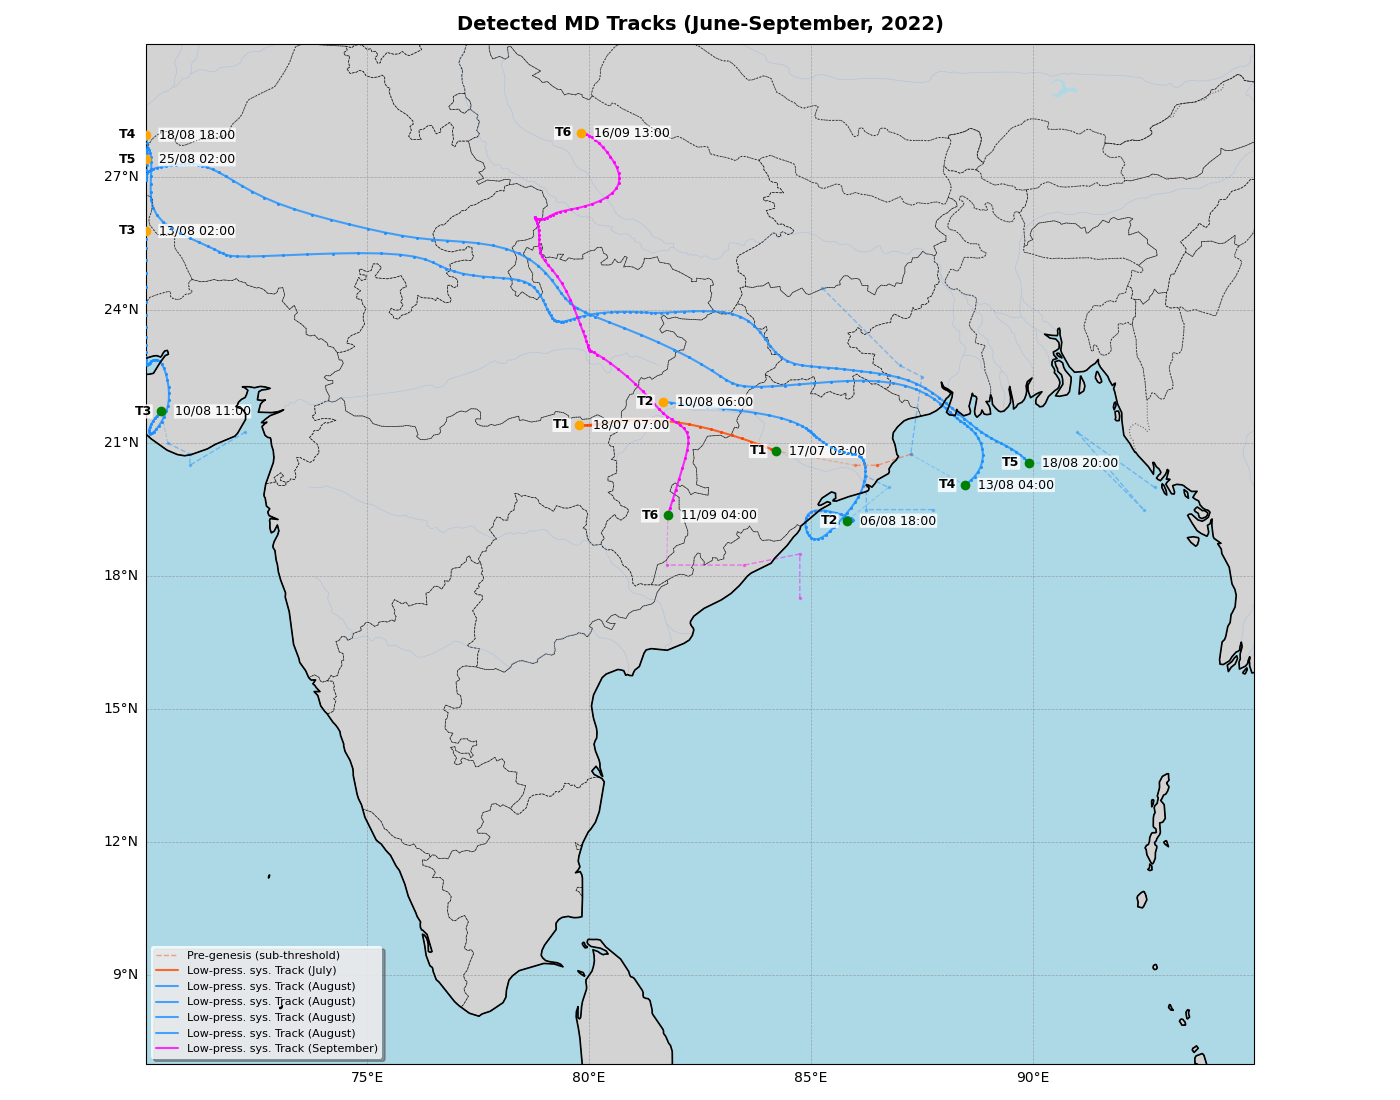
\includegraphics[width=1.2\textwidth]{MD_tracks_2022.png}
      \caption{2022 Monsoon Season}
    \end{subfigure}
    \hspace{0.11cm}
    \begin{subfigure}{0.52\textwidth}
      \centering
      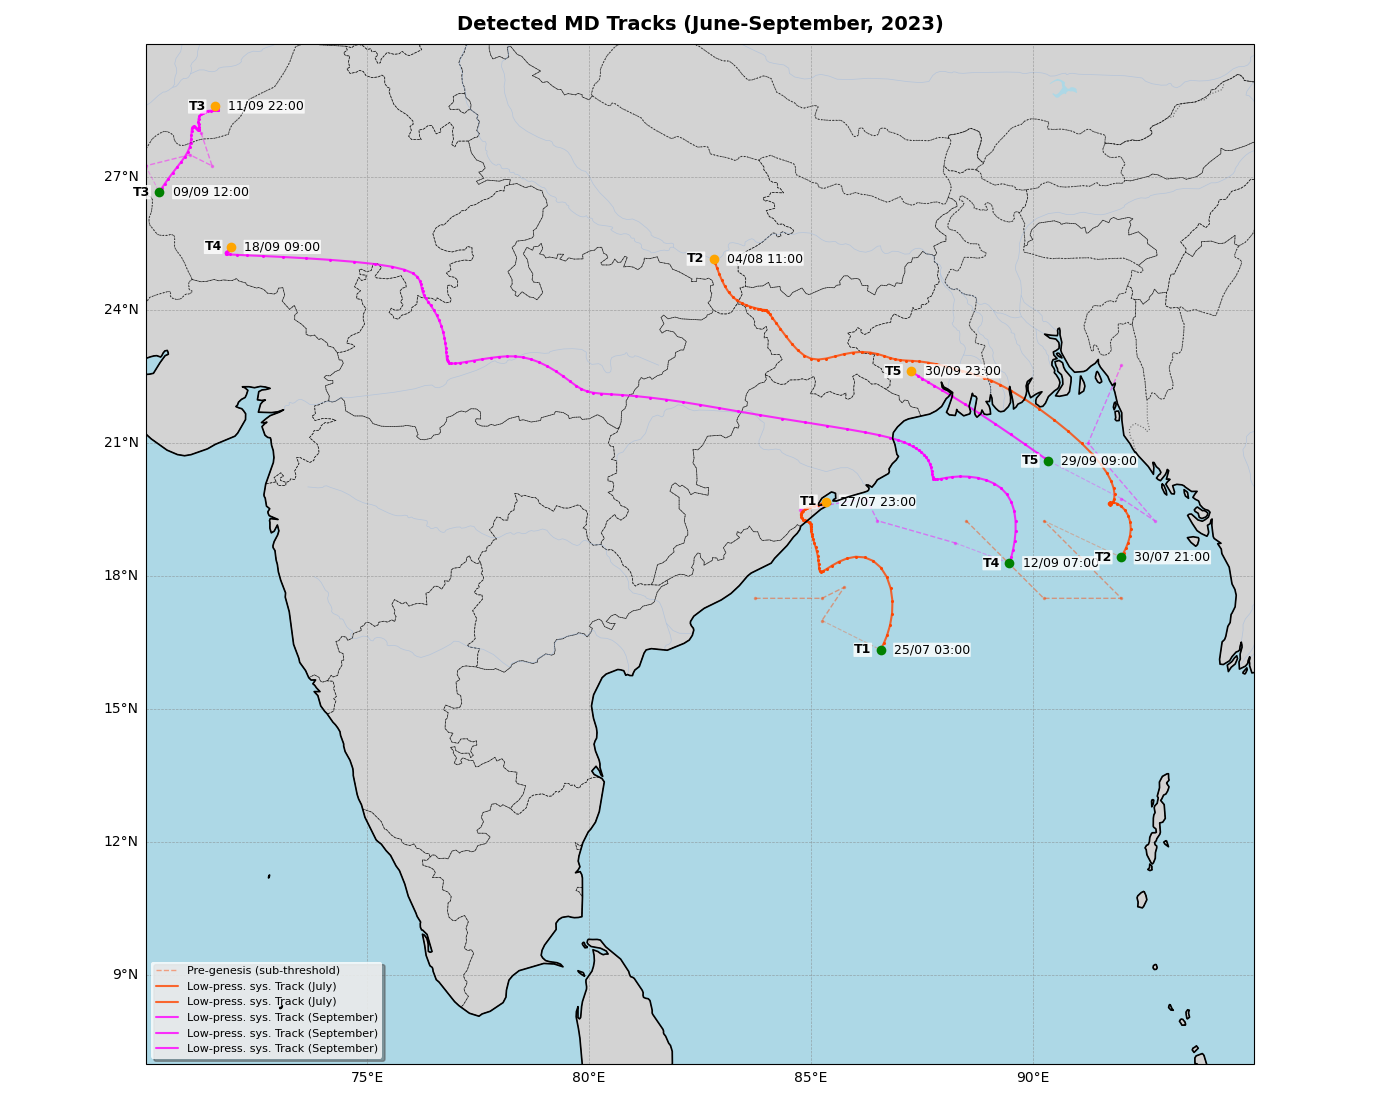
\includegraphics[width=1.2\textwidth]{MD_tracks_2023.png}
      \caption{2023 Monsoon Season}
    \end{subfigure}

    \vspace{0.9cm}

    \begin{subfigure}{0.52\textwidth}
      \centering
      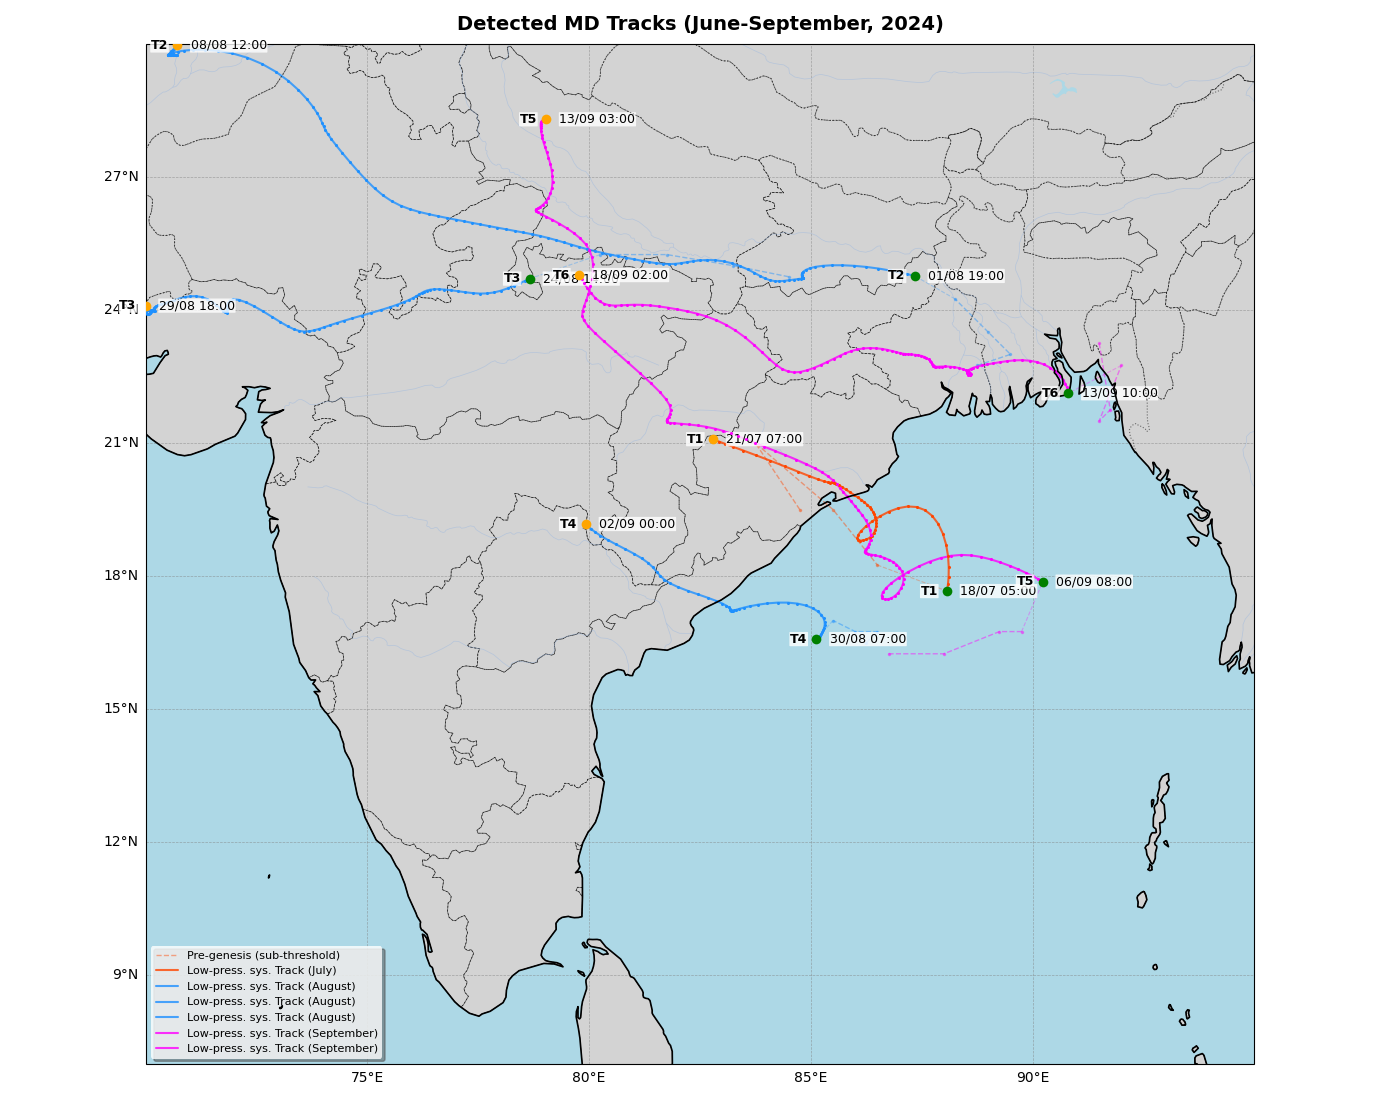
\includegraphics[width=1.2\textwidth]{MD_tracks_2024.png}
      \caption{2024 Monsoon Season}
    \end{subfigure}
    \hspace{0.11cm}
    \begin{subfigure}{0.52\textwidth}
      \centering
      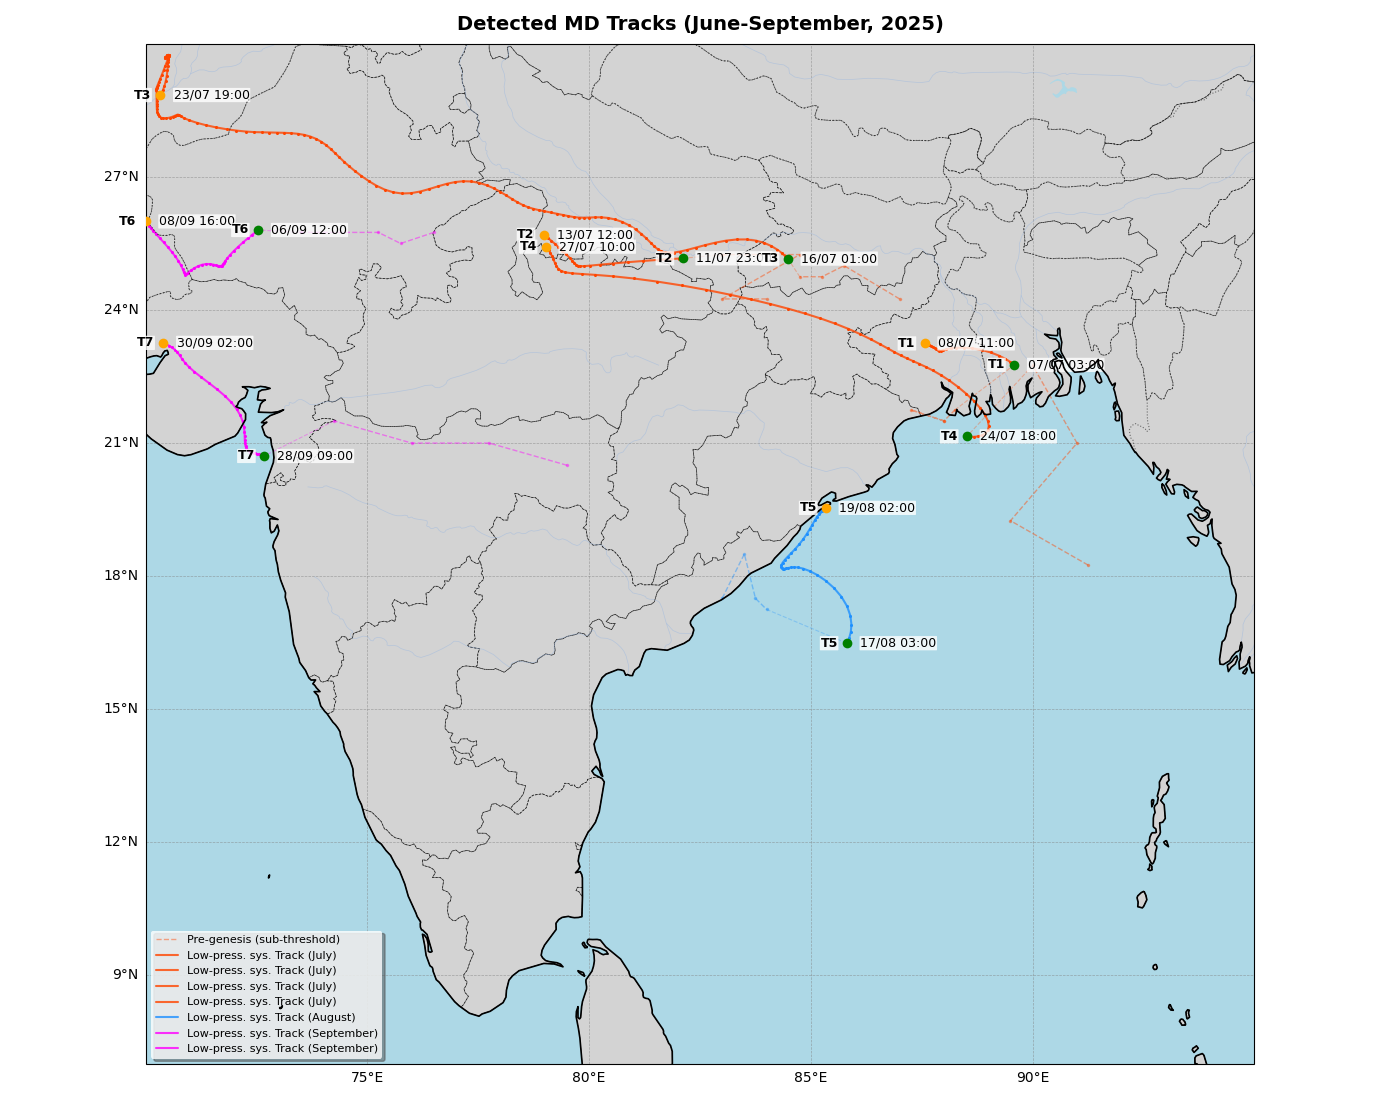
\includegraphics[width=1.2\textwidth]{MD_tracks_2025.png}
      \caption{2025 Monsoon Season}
    \end{subfigure}
    \caption{Annual MD Tracks: 2024-2025}
  \end{adjustwidth}
\end{figure}

% % Thesis Appendix B
\chapter{Storm-Centered Diagnostics}

\addcontentsline{toc}{chapter}{ B: MD-Centered Diagnostics (2001-2025)}
\chapter*{Appendix B: MD-Centered Diagnostics (2001-2025)}
\markboth{Appendix B: MD-Centered Diagnostics (2001-2025)}{ B:
MD-Centered Diagnostics (2001-2025) }



\includepdf[pages=-]{anc/plagiarism_report}
\end{document}
